% Options for packages loaded elsewhere
% Options for packages loaded elsewhere
\PassOptionsToPackage{unicode}{hyperref}
\PassOptionsToPackage{hyphens}{url}
\PassOptionsToPackage{dvipsnames,svgnames,x11names}{xcolor}
\PassOptionsToPackage{space}{xeCJK}
%
\documentclass[
  12pt,
  letterpaper,
  DIV=11,
  numbers=noendperiod]{scrartcl}
\usepackage{xcolor}
\usepackage[top=23mm, bottom=35mm, left=30mm, right=25mm]{geometry}
\usepackage{amsmath,amssymb}
\setcounter{secnumdepth}{-\maxdimen} % remove section numbering
\usepackage{iftex}
\ifPDFTeX
  \usepackage[T1]{fontenc}
  \usepackage[utf8]{inputenc}
  \usepackage{textcomp} % provide euro and other symbols
\else % if luatex or xetex
  \usepackage{unicode-math} % this also loads fontspec
  \defaultfontfeatures{Scale=MatchLowercase}
  \defaultfontfeatures[\rmfamily]{Ligatures=TeX,Scale=1}
\fi
\usepackage{lmodern}
\ifPDFTeX\else
  % xetex/luatex font selection
  \setmainfont[]{Times New Roman}
  \ifXeTeX
    \usepackage{xeCJK}
    \setCJKmainfont[AutoFakeSlant=0.15]{Noto Serif CJK TC}
  \fi
  \ifLuaTeX
    \usepackage[]{luatexja-fontspec}
    \setmainjfont[AutoFakeSlant=0.15]{Noto Serif CJK TC}
  \fi
\fi
% Use upquote if available, for straight quotes in verbatim environments
\IfFileExists{upquote.sty}{\usepackage{upquote}}{}
\IfFileExists{microtype.sty}{% use microtype if available
  \usepackage[]{microtype}
  \UseMicrotypeSet[protrusion]{basicmath} % disable protrusion for tt fonts
}{}
\makeatletter
\@ifundefined{KOMAClassName}{% if non-KOMA class
  \IfFileExists{parskip.sty}{%
    \usepackage{parskip}
  }{% else
    \setlength{\parindent}{0pt}
    \setlength{\parskip}{6pt plus 2pt minus 1pt}}
}{% if KOMA class
  \KOMAoptions{parskip=half}}
\makeatother
% Make \paragraph and \subparagraph free-standing
\makeatletter
\ifx\paragraph\undefined\else
  \let\oldparagraph\paragraph
  \renewcommand{\paragraph}{
    \@ifstar
      \xxxParagraphStar
      \xxxParagraphNoStar
  }
  \newcommand{\xxxParagraphStar}[1]{\oldparagraph*{#1}\mbox{}}
  \newcommand{\xxxParagraphNoStar}[1]{\oldparagraph{#1}\mbox{}}
\fi
\ifx\subparagraph\undefined\else
  \let\oldsubparagraph\subparagraph
  \renewcommand{\subparagraph}{
    \@ifstar
      \xxxSubParagraphStar
      \xxxSubParagraphNoStar
  }
  \newcommand{\xxxSubParagraphStar}[1]{\oldsubparagraph*{#1}\mbox{}}
  \newcommand{\xxxSubParagraphNoStar}[1]{\oldsubparagraph{#1}\mbox{}}
\fi
\makeatother


\usepackage{longtable,booktabs,array}
\usepackage{calc} % for calculating minipage widths
% Correct order of tables after \paragraph or \subparagraph
\usepackage{etoolbox}
\makeatletter
\patchcmd\longtable{\par}{\if@noskipsec\mbox{}\fi\par}{}{}
\makeatother
% Allow footnotes in longtable head/foot
\IfFileExists{footnotehyper.sty}{\usepackage{footnotehyper}}{\usepackage{footnote}}
\makesavenoteenv{longtable}
\usepackage{graphicx}
\makeatletter
\newsavebox\pandoc@box
\newcommand*\pandocbounded[1]{% scales image to fit in text height/width
  \sbox\pandoc@box{#1}%
  \Gscale@div\@tempa{\textheight}{\dimexpr\ht\pandoc@box+\dp\pandoc@box\relax}%
  \Gscale@div\@tempb{\linewidth}{\wd\pandoc@box}%
  \ifdim\@tempb\p@<\@tempa\p@\let\@tempa\@tempb\fi% select the smaller of both
  \ifdim\@tempa\p@<\p@\scalebox{\@tempa}{\usebox\pandoc@box}%
  \else\usebox{\pandoc@box}%
  \fi%
}
% Set default figure placement to htbp
\def\fps@figure{htbp}
\makeatother

\ifLuaTeX
  \usepackage{luacolor}
  \usepackage[soul]{lua-ul}
\else
  \usepackage{soul}
  \ifXeTeX
    % soul's \st doesn't work for CJK:
    \usepackage{xeCJKfntef}
    \renewcommand{\st}[1]{\sout{#1}}
  \fi
\fi

% definitions for citeproc citations
\NewDocumentCommand\citeproctext{}{}
\NewDocumentCommand\citeproc{mm}{%
  \begingroup\def\citeproctext{#2}\cite{#1}\endgroup}
\makeatletter
 % allow citations to break across lines
 \let\@cite@ofmt\@firstofone
 % avoid brackets around text for \cite:
 \def\@biblabel#1{}
 \def\@cite#1#2{{#1\if@tempswa , #2\fi}}
\makeatother
\newlength{\cslhangindent}
\setlength{\cslhangindent}{1.5em}
\newlength{\csllabelwidth}
\setlength{\csllabelwidth}{3em}
\newenvironment{CSLReferences}[2] % #1 hanging-indent, #2 entry-spacing
 {\begin{list}{}{%
  \setlength{\itemindent}{0pt}
  \setlength{\leftmargin}{0pt}
  \setlength{\parsep}{0pt}
  % turn on hanging indent if param 1 is 1
  \ifodd #1
   \setlength{\leftmargin}{\cslhangindent}
   \setlength{\itemindent}{-1\cslhangindent}
  \fi
  % set entry spacing
  \setlength{\itemsep}{#2\baselineskip}}}
 {\end{list}}
\usepackage{calc}
\newcommand{\CSLBlock}[1]{\hfill\break\parbox[t]{\linewidth}{\strut\ignorespaces#1\strut}}
\newcommand{\CSLLeftMargin}[1]{\parbox[t]{\csllabelwidth}{\strut#1\strut}}
\newcommand{\CSLRightInline}[1]{\parbox[t]{\linewidth - \csllabelwidth}{\strut#1\strut}}
\newcommand{\CSLIndent}[1]{\hspace{\cslhangindent}#1}



\setlength{\emergencystretch}{3em} % prevent overfull lines

\providecommand{\tightlist}{%
  \setlength{\itemsep}{0pt}\setlength{\parskip}{0pt}}



 


\usepackage{graphicx}
% \usepackage{background}      % For background images
\usepackage[normalem]{ulem}  % For underlining
\usepackage{appendix}        % For appendix support
\usepackage{chngcntr}        % For resetting counters
\usepackage{pdfpages} 
\usepackage{booktabs}
\usepackage[flushleft]{threeparttable}

% Background image setup
% \backgroundsetup{
%   scale=1,
%   color=black,
%   opacity=1,
%   angle=0,
%   position=current page.center,
%   vshift=0cm,
%   hshift=0cm,
%   contents={
\includegraphics[width=0.2\paperwidth]{images/watermark.png}}
% }

% add to cover -> \NoBgThispage 

% Set numbering depth to include \paragraph
\setcounter{secnumdepth}{4}
\setcounter{tocdepth}{4}

% Customize \section (Chapter-Level Headings)
\RedeclareSectionCommand[
  beforeskip=1em plus 0.5em minus 0.2em,
  afterskip=1em,
  indent=0pt,
  font=\normalfont\bfseries\centering\MakeUppercase
]{section}

% Customize \subsection (First-Level Subheadings)
\RedeclareSectionCommand[
  beforeskip=1em plus 0.5em minus 0.2em,
  afterskip=1em,
  indent=0pt,
  font=\normalfont\bfseries\centering
]{subsection}

% Customize \subsubsection (Second-Level Subheadings)
\RedeclareSectionCommand[
  beforeskip=1em plus 0.5em minus 0.2em,
  afterskip=1em,
  indent=0pt,
  font=\normalfont\bfseries
]{subsubsection}

% Customize \paragraph (Third-Level Subheadings)
\RedeclareSectionCommand[
  beforeskip=1em plus 0.5em minus 0.2em,
  afterskip=1em,
  indent=0pt,
  afterindent=false, % Do not indent the first paragraph
  font=\normalfont\underline,
  level=4,
  style=section
]{paragraph}

% Adjust numbering in the appendix
\newcommand{\appendixnumbering}{
  \renewcommand{\thesection}{\Alph{section}}
  \renewcommand{\thesubsection}{\thesection.\arabic{subsection}}
  \renewcommand{\thesubsubsection}{\thesubsection.\arabic{subsubsection}}
  \renewcommand{\theparagraph}{\thesubsubsection.\arabic{paragraph}}
  \setcounter{section}{0}
  \setcounter{subsection}{0}
  \setcounter{subsubsection}{0}
  \setcounter{paragraph}{0}
}

% keep the real command
\let\SavedLoT\listoftables
% replace the auto page with an empty stub
\renewcommand{\listoftables}{}\KOMAoption{captions}{tableheading}
% -- begin:latex-table-short-captions --
\makeatletter\AtBeginDocument{%
\def\LT@c@ption#1[#2]#3{%                 % Overwrite the workhorse macro used in formatting a longtable caption.
  \LT@makecaption#1\fnum@table{#3}%
  \@ifundefined{pandoctableshortcapt}
     {\def\@tempa{#2}}                    % Use default behaviour: argument in square brackets
     {\let\@tempa\pandoctableshortcapt}   % If defined (even if blank), use to override
  \ifx\@tempa\@empty\else                 % If @tempa is blank, no lot entry! Otherwise, @tempa becomes the lot title.
     {\let\\\space
     \addcontentsline{lot}{table}{\protect\numberline{\thetable}{\@tempa}}}%
  \fi}
}\makeatother
% -- end:latex-table-short-captions --
\makeatletter
\@ifpackageloaded{caption}{}{\usepackage{caption}}
\AtBeginDocument{%
\ifdefined\contentsname
  \renewcommand*\contentsname{Table of contents}
\else
  \newcommand\contentsname{Table of contents}
\fi
\ifdefined\listfigurename
  \renewcommand*\listfigurename{List of Figures}
\else
  \newcommand\listfigurename{List of Figures}
\fi
\ifdefined\listtablename
  \renewcommand*\listtablename{List of Tables}
\else
  \newcommand\listtablename{List of Tables}
\fi
\ifdefined\figurename
  \renewcommand*\figurename{Figure}
\else
  \newcommand\figurename{Figure}
\fi
\ifdefined\tablename
  \renewcommand*\tablename{Table}
\else
  \newcommand\tablename{Table}
\fi
}
\@ifpackageloaded{float}{}{\usepackage{float}}
\floatstyle{ruled}
\@ifundefined{c@chapter}{\newfloat{codelisting}{h}{lop}}{\newfloat{codelisting}{h}{lop}[chapter]}
\floatname{codelisting}{Listing}
\newcommand*\listoflistings{\listof{codelisting}{List of Listings}}
\makeatother
\makeatletter
\makeatother
\makeatletter
\@ifpackageloaded{caption}{}{\usepackage{caption}}
\@ifpackageloaded{subcaption}{}{\usepackage{subcaption}}
\makeatother
\usepackage{bookmark}
\IfFileExists{xurl.sty}{\usepackage{xurl}}{} % add URL line breaks if available
\urlstyle{same}
\hypersetup{
  colorlinks=true,
  linkcolor={black},
  filecolor={Maroon},
  citecolor={black},
  urlcolor={black},
  pdfcreator={LaTeX via pandoc}}


\author{}
\date{}
\begin{document}

\listoftables

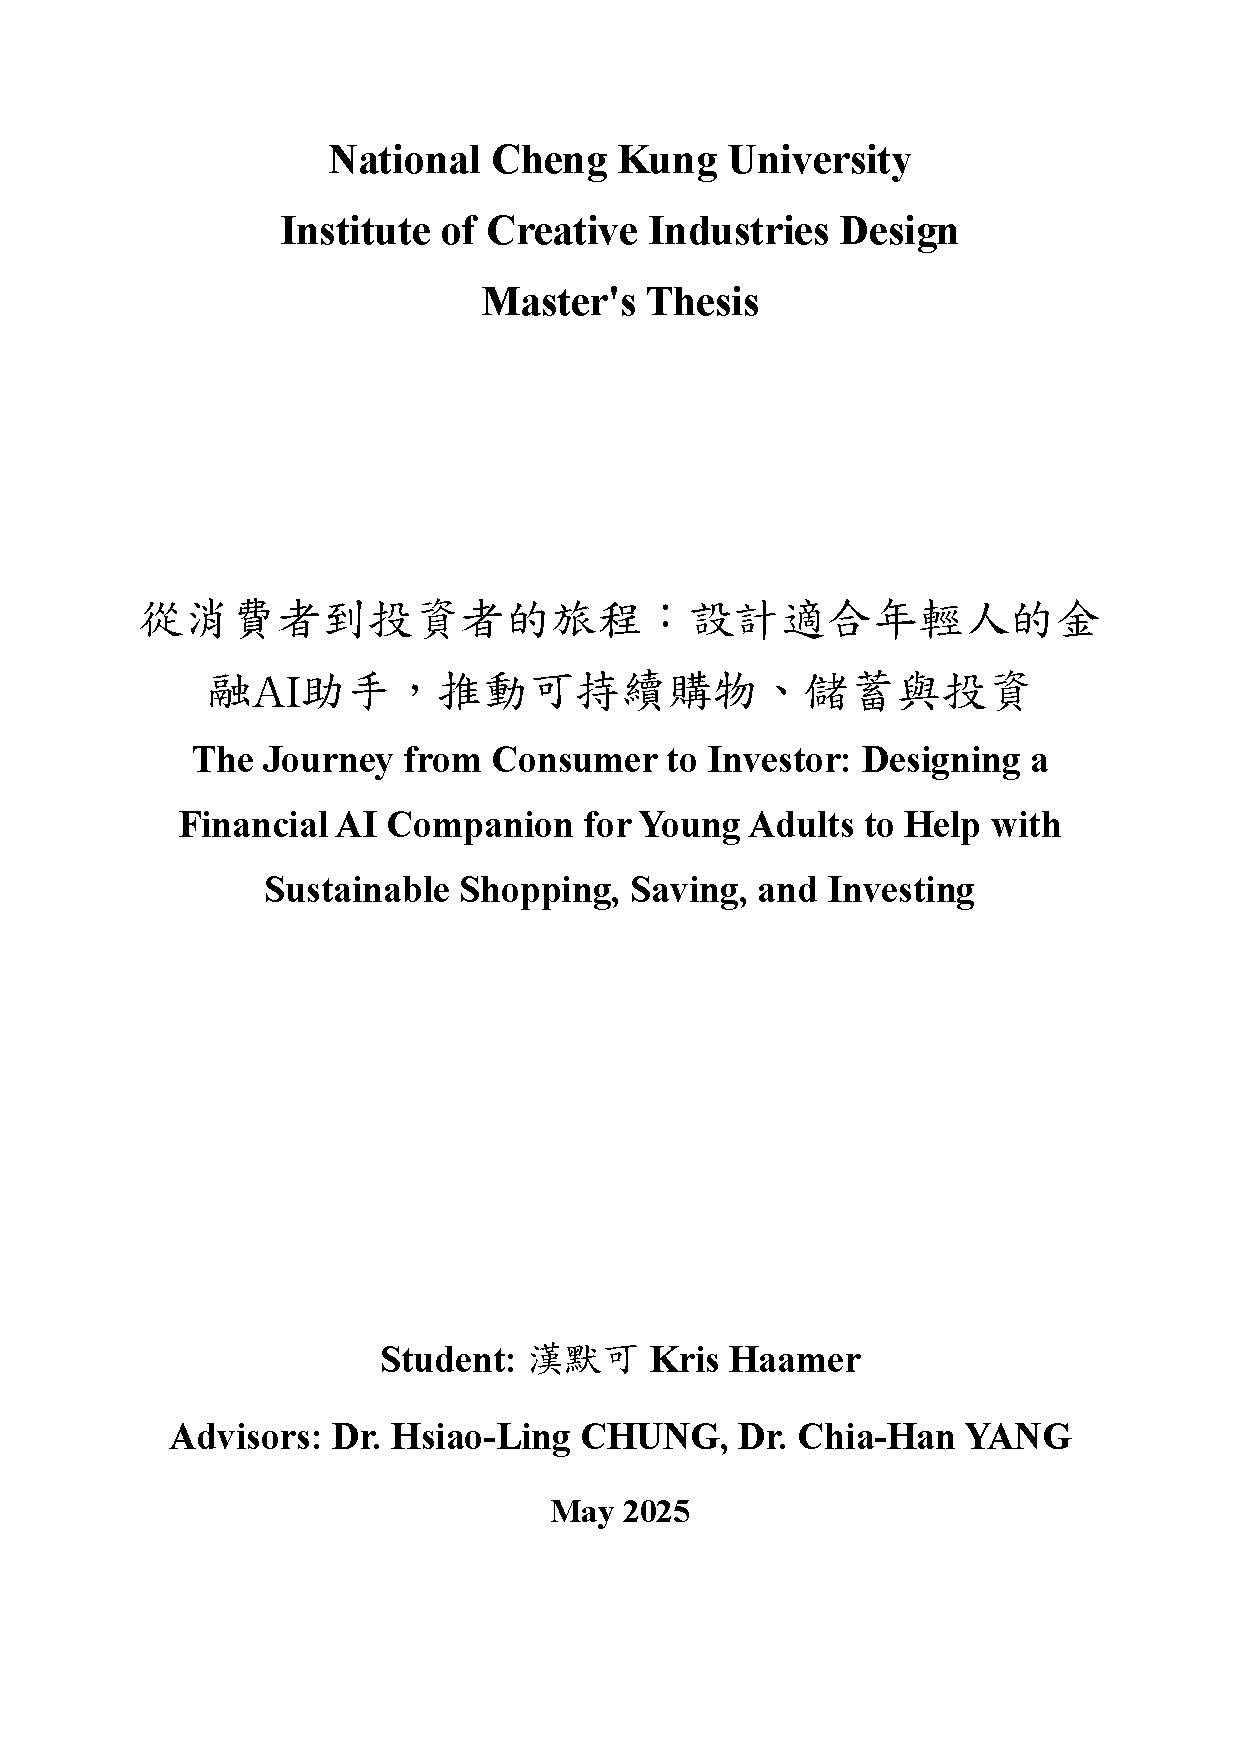
\includepdf[
  pages=1,
  fitpaper=true,
  pagecommand={\thispagestyle{empty}}
]{_cover.pages.pdf}
\clearpage

\newpage

\section{Abstract}\label{abstract}

As of 2025, Earth's natural environment is being heavily degraded by the
extractive business practices of companies that make many of the
products and services we buy every day. The emerging field of
\emph{planetary health} recognizes profound interconnections between our
economic behaviors, ecosystem services such as clean water, air, soil,
the climate crisis, and human health. The way we use money to interact
with companies - through shopping, or saving and investing - impacts the
life-supporting biosphere we depend on. In essence, from an ecological
perspective, every financial action is either an investment decision to
support more environmentally-friendly companies - or to support
polluters.

In Taiwan, college students are concerned with environmental issues, yet
lack simple tools to effectively influence systemic change towards
sustainable outcomes. Concurrently, in the European Union, new
environmental policies include the concept of \emph{digital product
passports (DPPs)}, which aim to facilitate tracking data across the
entire product lifecycle, from source materials, until the consumer
purchase decision, and finally post-purchase recycling, building
\emph{transparency} into opaque global supply chains. These new digital
tools hold the potential to benefit from \emph{data-driven interaction
design}, \emph{large-language models}, and \emph{AI agents} to translate
complex environmental data into human-comprehensible language. If
successful, DPPs may help to solve the \emph{attitude-behavior gap} by
making it easy to distinguish \emph{eco-designed products} made by
circular economy companies, striving to be \emph{zero waste}, from those
merely engaged in \emph{greenwashing}.

My research focuses on college students and addresses the need for tools
to make sustainable financial action more convenient. I leverage
\emph{design research} to find design concepts for \emph{simple AI-based
generative user interfaces} to help young adults participate in
\emph{sustainable financial activism}. Throughout the process, I
conducted a survey of over 900 students from 20 universities across
Taiwan, face-to-face user testing with 30 participants, and 6 expert
interviews providing industry insights. The major contribution of the
study is an interactive AI-assistant prototype.

Keywords: Human-AI Interaction, Digital Sustainability, Transparency

\newpage

\section{摘要}\label{ux6458ux8981}

台灣的年輕人,特別是大學生,關注環境問題,但因缺乏簡單的工具來影響系統性改變而受阻。同時,歐盟加強的環保政策引入了「數字產品護照」的概念,旨在區分由努力實現零廢棄的「循環經濟」公司製造的「生態設計」產品,與僅從事「漂綠」的公司。從原料開始追蹤產品數據,直到消費者的購買決策,最後到購後的回收,促進在不透明的全球供應鏈中建立透明度。
「數據驅動的互動設計」、「大型語言模型」和「人工智慧助理」將復雜的環境數據轉換成人類可理解的語言。

新興的「地球健康」領域認識到,我們的經濟行為、生態系統服務(如清潔的水、空氣、土壤)、氣候危機和人類健康之間存在著深刻的相互聯繫。截至2024年,由於生產我們日常購買的許多產品和服務的公司進行的開採性商業行為,地球的自然環境正被嚴重破壞。我們用金錢與公司互動的方式------作為消費者的購物和作為投資者的儲蓄/投資------對我們賴以維持地球宜居性的生命支持生物圈產生影響。從生態學角度來看,每一個財務行動不是支持更環保公司的投資決策,就是支持污染者。透過民主化金融市場,年輕人可以獲得更大的權限和影響力,控制他們的資金流向,使他們能夠支持可持續和對環境負責的公司。

我的研究針對了需要工具來使可持續的財務行動更便捷的需求,特別關注大學生。我利用設計研究來尋找簡單的基於AI的使用者介面的設計概念,也稱為生成式UI,以幫助年輕人參與可持續的財務行動主義。在台灣10所大學進行了涵蓋700名學生的調查,並透過5次專家訪談提供行業見解。研究的主要貢獻是一個互動式AI助理原型。

關鍵詞:人機互動、數字可持續性、透明度

\emph{The abstract was translated on May 22, 2024 using the Claude 3
Opus model. Translation quality was checked with OpenAI GPT4, Google
Gemini, Mistral Large, Meta LLama, as well as human reviewers, and
further refined with the OpenAI o1-preview model in November 2024. In
case of any discrepancies, please refer to the English text.}

\newpage

\section{Acknowledgments}\label{acknowledgments}

Thank you mom. Aitäh.

I'd like to express my gratitude to my entire family, 小猴子, professors
and mentors. Thank you all for your patience, help and guidance.

\newpage

\tableofcontents
\clearpage 
\listoffigures
\clearpage 
\SavedLoT

\newpage

\section{List of Symbols and
Abbreviations}\label{list-of-symbols-and-abbreviations}

Some of the key terminology used in my thesis presented in a concise
format.

\begin{enumerate}
\def\labelenumi{\arabic{enumi}.}
\item
  AI - Artificial intelligence, a field of computer science and an
  umbrella term focused on a wide range of approaches to automation
\item
  UX - User experience, a field of study and operational approach
  focused on how humans experience using systems
\item
  AX - Algorithmic experience, a proposed category of user experience,
  that is focused on interfaces between AI algorithms and humans
\item
  UI - User interface, such as in a mobile app, however increasingly
  audio, video, etc
\item
  XAI - AI user experience, interaction design applied to AI concerned
  with how does a person or a group of people interact with the AI
\item
  Fintech - Financial technology, the application of technology (usually
  AI), to classic financial services, such as payments
\item
  ESG - Environmental, Social, and Corporate Governance, a new set of
  metrics proposed by the European Union, and adopted worldwide, to
  assess business and financial assets
\item
  AI Assistant - software system providing the user with personalized
  suggestions based on machine learning algorithms
\item
  Financial Advisor - a human financial specialist providing customized
  financial advice, including investment advice and services to a client
\item
  ML - Machine learning, a tool within the larger AI umbrella to enable
  computers to learn from large sets of data, which may be labeled (by
  humans) or un-labeled (auto-labeled)
\item
  HCI - Human-computer interaction, a field of study to improve human
  experience with information technology
\item
  OEM - Original equipment manufacturer, a company making products for
  another company that markets and sells such products under their own
  brand
\item
  API - Application Programming Interface, a method for software agents
  to exchange information in various forms of data: the basis for
  contemporary online services
\item
  EPR - Extended Producer Responsibility
\item
  SDGs - Sustainable Development Goals, a set of targets agreed upon by
  the nations of the world
\item
  LLM - Large Language Models
\item
  Vector Databases - specialized data storage for mathematical language
  embeddings in multi-dimensional space helpful for clustering similar
  concepts
\item
  CO\textsubscript{2}eq - CO\textsubscript{2} equivalent greenhouse
  gases
\item
  GHG - Greenhause gases
\item
  PD - Participatory Design
\item
  VCM - Voluntary Carbon Markets
\item
  Hedge Fund - pooled investment fund
\item
  DAO - Decentralized Autonomous Organization
\item
  Zero Waste - according to Zero Waste International Alliance:
  \emph{``conservation of all resources by means of responsible
  production, consumption, reuse and recovery of products, packaging and
  materials without burning, and with no discharges to land, water or
  air that threaten the environment or human health''} - (Kalle et al.,
  2022)
\item
  ESPR - Ecodesign for Sustainable Products Regulation
\item
  NFRD - Non-Financial Reporting Directive
\item
  CSRD - Corporate Sustainability Reporting Directive
\item
  EUDR - European Union Deforestation Regulation
\item
  Product Stewardship
\item
  Extended Producer Responsibility
\end{enumerate}

\newpage

\section{Introduction}\label{introduction}

How can college students find sustainable companies? Furthermore, if
given appropriate tools, could college students leverage their
purchasing power to reward sustainable companies? Why is this important
to research now? Young people should invest in their future and younger
generations like services with a green, eco-conscious focus. Given our
combined power (I'm a Millennial) with Generation Z, we are willing to
pay more for sustainable products. Does Individual Climate Action
Matter?

My research describes the process of designing an AI companion for
college students to help with sustainable shopping, saving, and
investing. Money spent shopping, saving, and investing in sustainable
companies serves as an incentive to adopt more sustainable practices. If
used wisely, money can reward companies for becoming more sustainable.
Encourage the least sustainable companies to improve their performance,
raising the overall baseline. Facilitate the formation of communities
centered around environmental stewardship. Build closer relationships
with sustainability.

\begin{figure}[H]

{\centering 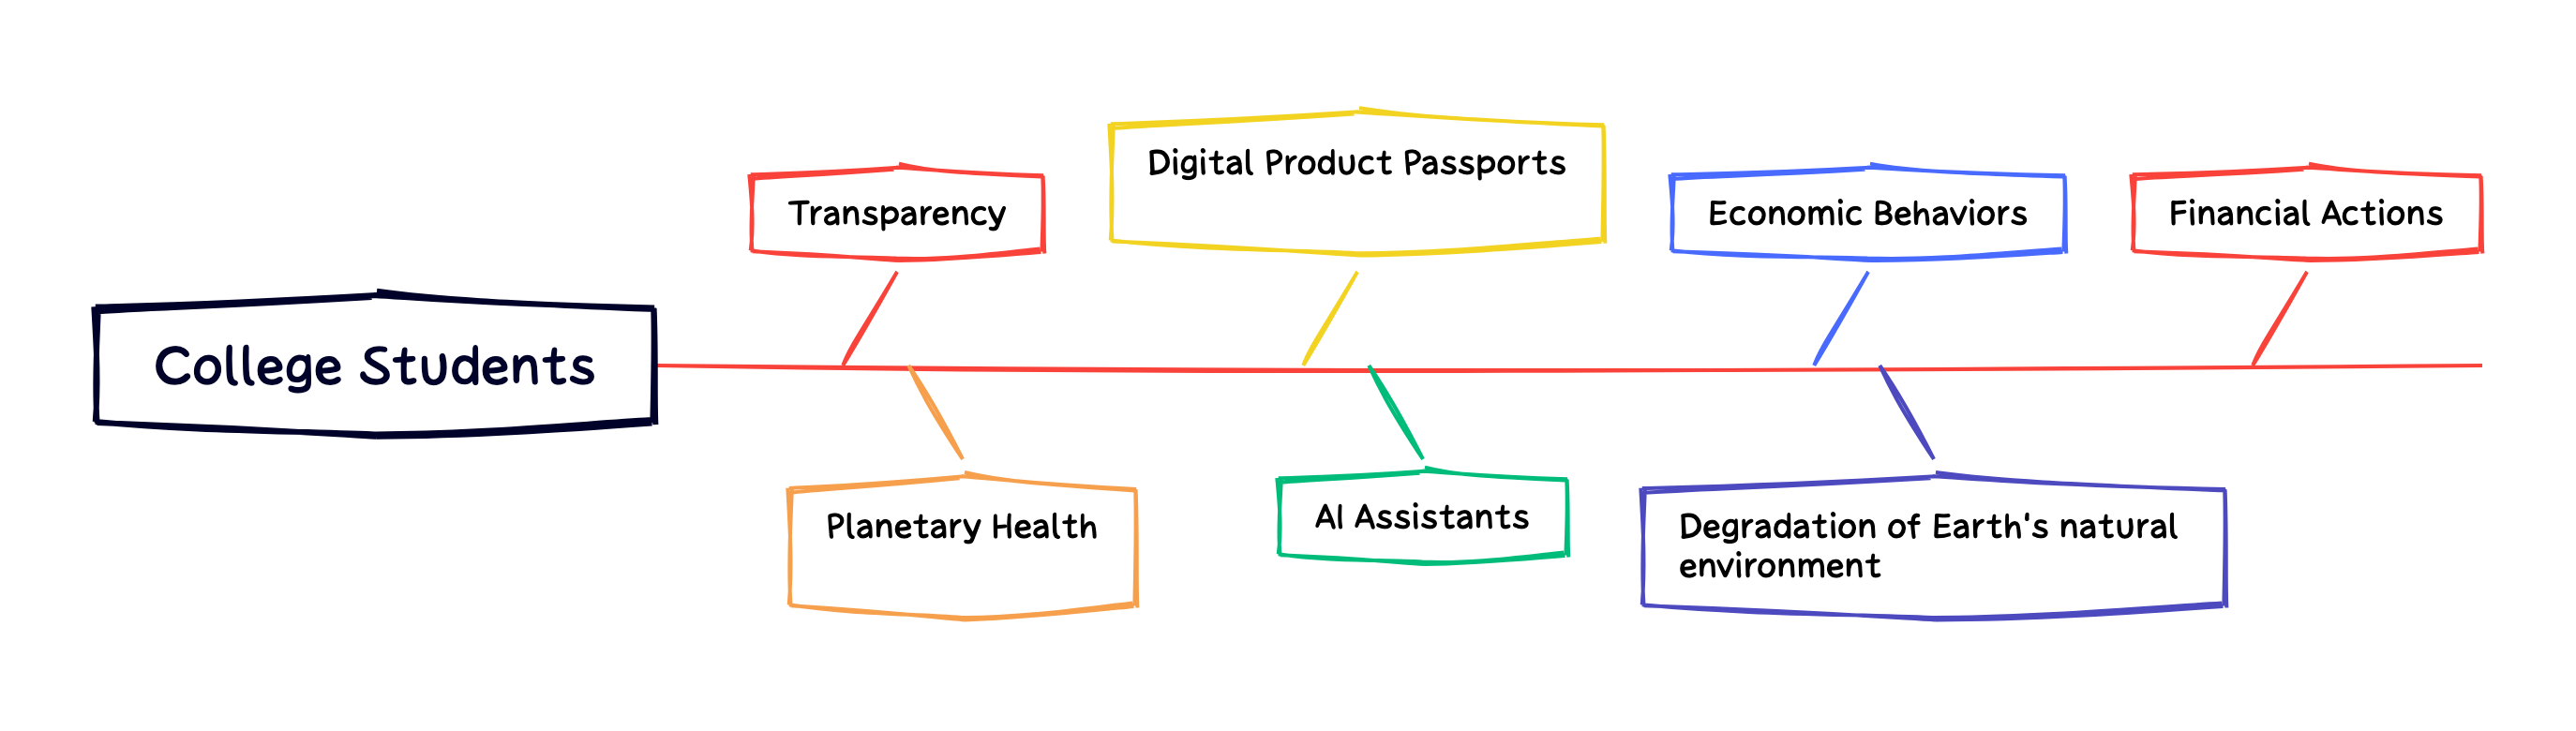
\includegraphics[width=1\linewidth,height=\textheight,keepaspectratio]{./images/introduction/abstract.png}

}

\caption{College Students}

\end{figure}%

\subsection{Relevance}\label{relevance}

The research addresses the \emph{``attitude-behavior gap''} among
Taiwanese college students in taking sustainable financial action.
Convergence of the following 5 trends makes my research timely in 2024.

\begin{longtable}[]{@{}
  >{\raggedright\arraybackslash}p{(\linewidth - 2\tabcolsep) * \real{0.4167}}
  >{\raggedright\arraybackslash}p{(\linewidth - 2\tabcolsep) * \real{0.5833}}@{}}
\caption{Trending Narratives.}\tabularnewline
\toprule\noalign{}
\begin{minipage}[b]{\linewidth}\raggedright
Trend
\end{minipage} & \begin{minipage}[b]{\linewidth}\raggedright
Direction
\end{minipage} \\
\midrule\noalign{}
\endfirsthead
\toprule\noalign{}
\begin{minipage}[b]{\linewidth}\raggedright
Trend
\end{minipage} & \begin{minipage}[b]{\linewidth}\raggedright
Direction
\end{minipage} \\
\midrule\noalign{}
\endhead
\bottomrule\noalign{}
\endlastfoot
Environmental degradation & Worsening \\
Interest in sustainability among young people & ? \\
Intergenerational money transfer; in some countries relatively young
people have money & ? \\
Availability of sustainability tools such as ESG, B Corporations, Green
Bonds, etc, among metrics and instruments & Increasing \\
Availability of generative AI-based user interfaces (UIs) &
Increasing \\
Democratization of Financial Markets & Increasing \\
\end{longtable}

\subsection{Background}\label{background}

I grew up as an avid science fiction reader, which influenced my outlook
towards future possibilities. In particular, the Star Trek universe had
an imaginary portable device called a \textbf{\emph{tricorder}} (fig.~1)
enabling scientists to scan anything for insights. Be it precious
minerals inside a cave or scanning the human bodies for medical data,
its sensors would show up with some useful data. In daily life, I would
love to have such a device for consumer choices and financial decisions
- to know what to buy and which businesses to support with my money and
approval.

\begin{figure}

\centering{


\includegraphics[width=0.5\linewidth,height=\textheight,keepaspectratio]{./images/introduction/tricorder.jpg}

}

\caption{\label{fig-co2-tricorder}Captain Sulu using a Tricorder (Star
Trek) - Photo copyright by Paramount Pictures}

\end{figure}%

While a \emph{tricorder} is still science fiction, technological
advancements are getting closer and closer to producing something
similar. AIs are already integral to many parts of our lives, with
computer models producing increasingly useful outputs. The proposal for
this thesis was first written using Google's and Apple's voice
recognition software in 2020, and later switching to OpenAI's
\emph{Whisper} model, allowing me to transcribe notes with the help of
an AI assistant. As a foreigner living in Taiwan since 2019, I relied on
AI-based tools for many aspects of my life: speaking, moving, finding
food and services. When writing in Chinese, Apple's text prediction
algorithms translate pinyin to 漢字 and show the most likely character
based on my previous writing, Google's maps find efficient and
eco-friendly routes and recommend places to eat and ChatGPT provides
statistically probable advice from the sum of human knowledge. Even when
we don't realize it, AI is helping us with many mundane tasks. While it
takes incredibly complex computational algorithms to achieve all this in
the background, it's become so commonplace, we don't even think about
it. From this point of view, another AI assistant to help students with
choosing more eco-friendly businesses - to shop, save, and invest -
doesn't sound so much of a stretch.

\subsection{Motivation}\label{motivation}

Environmental degradation is increasingly affecting human lives - and
it's largely driven by manufacturing processes - of the products we
consume daily. From resource extraction in the linear economy (mining
raw materials and drilling for fossil fuels) to chemical processes
(causing contamination and pollution of the air, water, and soil) to
waste generation and greenhouse gas emissions, industries transform the
natural world into consumer products. While industry practices have
improved since the industrial revolution in the 19th century, and
continue to improve, it's possible to further improve standards of
production and raise the global baseline for sustainability, given
enough societal pressure to do so.

Nonetheless, without easily accessible and reliable data, it's difficult
to know which company is more sustainable than another. As consumers and
investors (even if only through passive ownership of savings), we don't
really know much about enterprise production practices, unless we spend
a lot of time looking at the numbers, which may be costly to access (for
example ESG reports are expensive), and mostly rely on our governments
and international bodies to keep us safe. Or just look at the brands
themselves - and pick the ones which we like.

\subsection{Objective}\label{objective}

The study presents design research for developing an AI companion to
help college students find sustainable companies for shopping, saving
and investing. The major contribution of my study is an interactive
artefact (a prototype) informed by design research.

\subsection{Demographics}\label{demographics}

The research focuses on young adults, specifically Taiwanese college
students studying in Taiwan.

\begin{longtable}[]{@{}ll@{}}
\toprule\noalign{}
Criteria & \\
\midrule\noalign{}
\endhead
\bottomrule\noalign{}
\endlastfoot
Location & Taiwan \\
Population & College Students \\
Count & 700 \\
\end{longtable}

Experts (finance, design, sustainability).

\begin{longtable}[]{@{}ll@{}}
\toprule\noalign{}
Criteria & \\
\midrule\noalign{}
\endhead
\bottomrule\noalign{}
\endlastfoot
Location & Global \\
Population & Experts \\
Count & 5 \\
\end{longtable}

\subsection{Research Questions}\label{research-questions}

My research answers the following questions.

\begin{longtable}[]{@{}
  >{\raggedright\arraybackslash}p{(\linewidth - 2\tabcolsep) * \real{0.5556}}
  >{\raggedright\arraybackslash}p{(\linewidth - 2\tabcolsep) * \real{0.4444}}@{}}
\caption{Research Questions}\tabularnewline
\toprule\noalign{}
\begin{minipage}[b]{\linewidth}\raggedright
Question
\end{minipage} & \begin{minipage}[b]{\linewidth}\raggedright
Methods
\end{minipage} \\
\midrule\noalign{}
\endfirsthead
\toprule\noalign{}
\begin{minipage}[b]{\linewidth}\raggedright
Question
\end{minipage} & \begin{minipage}[b]{\linewidth}\raggedright
Methods
\end{minipage} \\
\midrule\noalign{}
\endhead
\bottomrule\noalign{}
\endlastfoot
What design considerations should be addressed when designing an AI
companion for college students integrating sustainability and finance? &
Literature Review \\
How can AI companions support college students with sustainability
knowledge in the context of financial decisions? & Literature Review and
Expert Interviews \\
What AI companion features do college students prioritize as the
highest? & Survey of College Students \\
\end{longtable}

\newpage

\subsection{Literature Review}\label{literature-review}

\subsubsection{Goals}\label{goals}

Given the goal of designing an app to integrate sustainable shopping,
saving, and investing. The goal of the literature review is to find
insights about the target audience (Taiwanese college students),
understand what kind of sustainable actions are effective, and translate
these into specific ideas for app features. In order to keep track more
easily, each literature review chapter provides \emph{design
implications} which are shown in the results section.

The literature review branches out to 5 main directions and maps out
relationships sources and the literature map, namely Taiwanese college
students, generation-z demographics, sustainability, ecology, ecosystem
services, EU legislation, sustainable finance, sustainable investing,
savings, circular economy, economics, AI, existing sustainability,
software, sustainability--related mobile apps (Apple iOS / Google
Android), and web apps related to sustainable shopping, savings, and
investing; apps using algorithmic interfaces (AI-based UI), design,
UX/UI, service design, sustainable design, speculative design,
interaction design, behavior change, nudge.

\begin{figure}[H]

{\centering 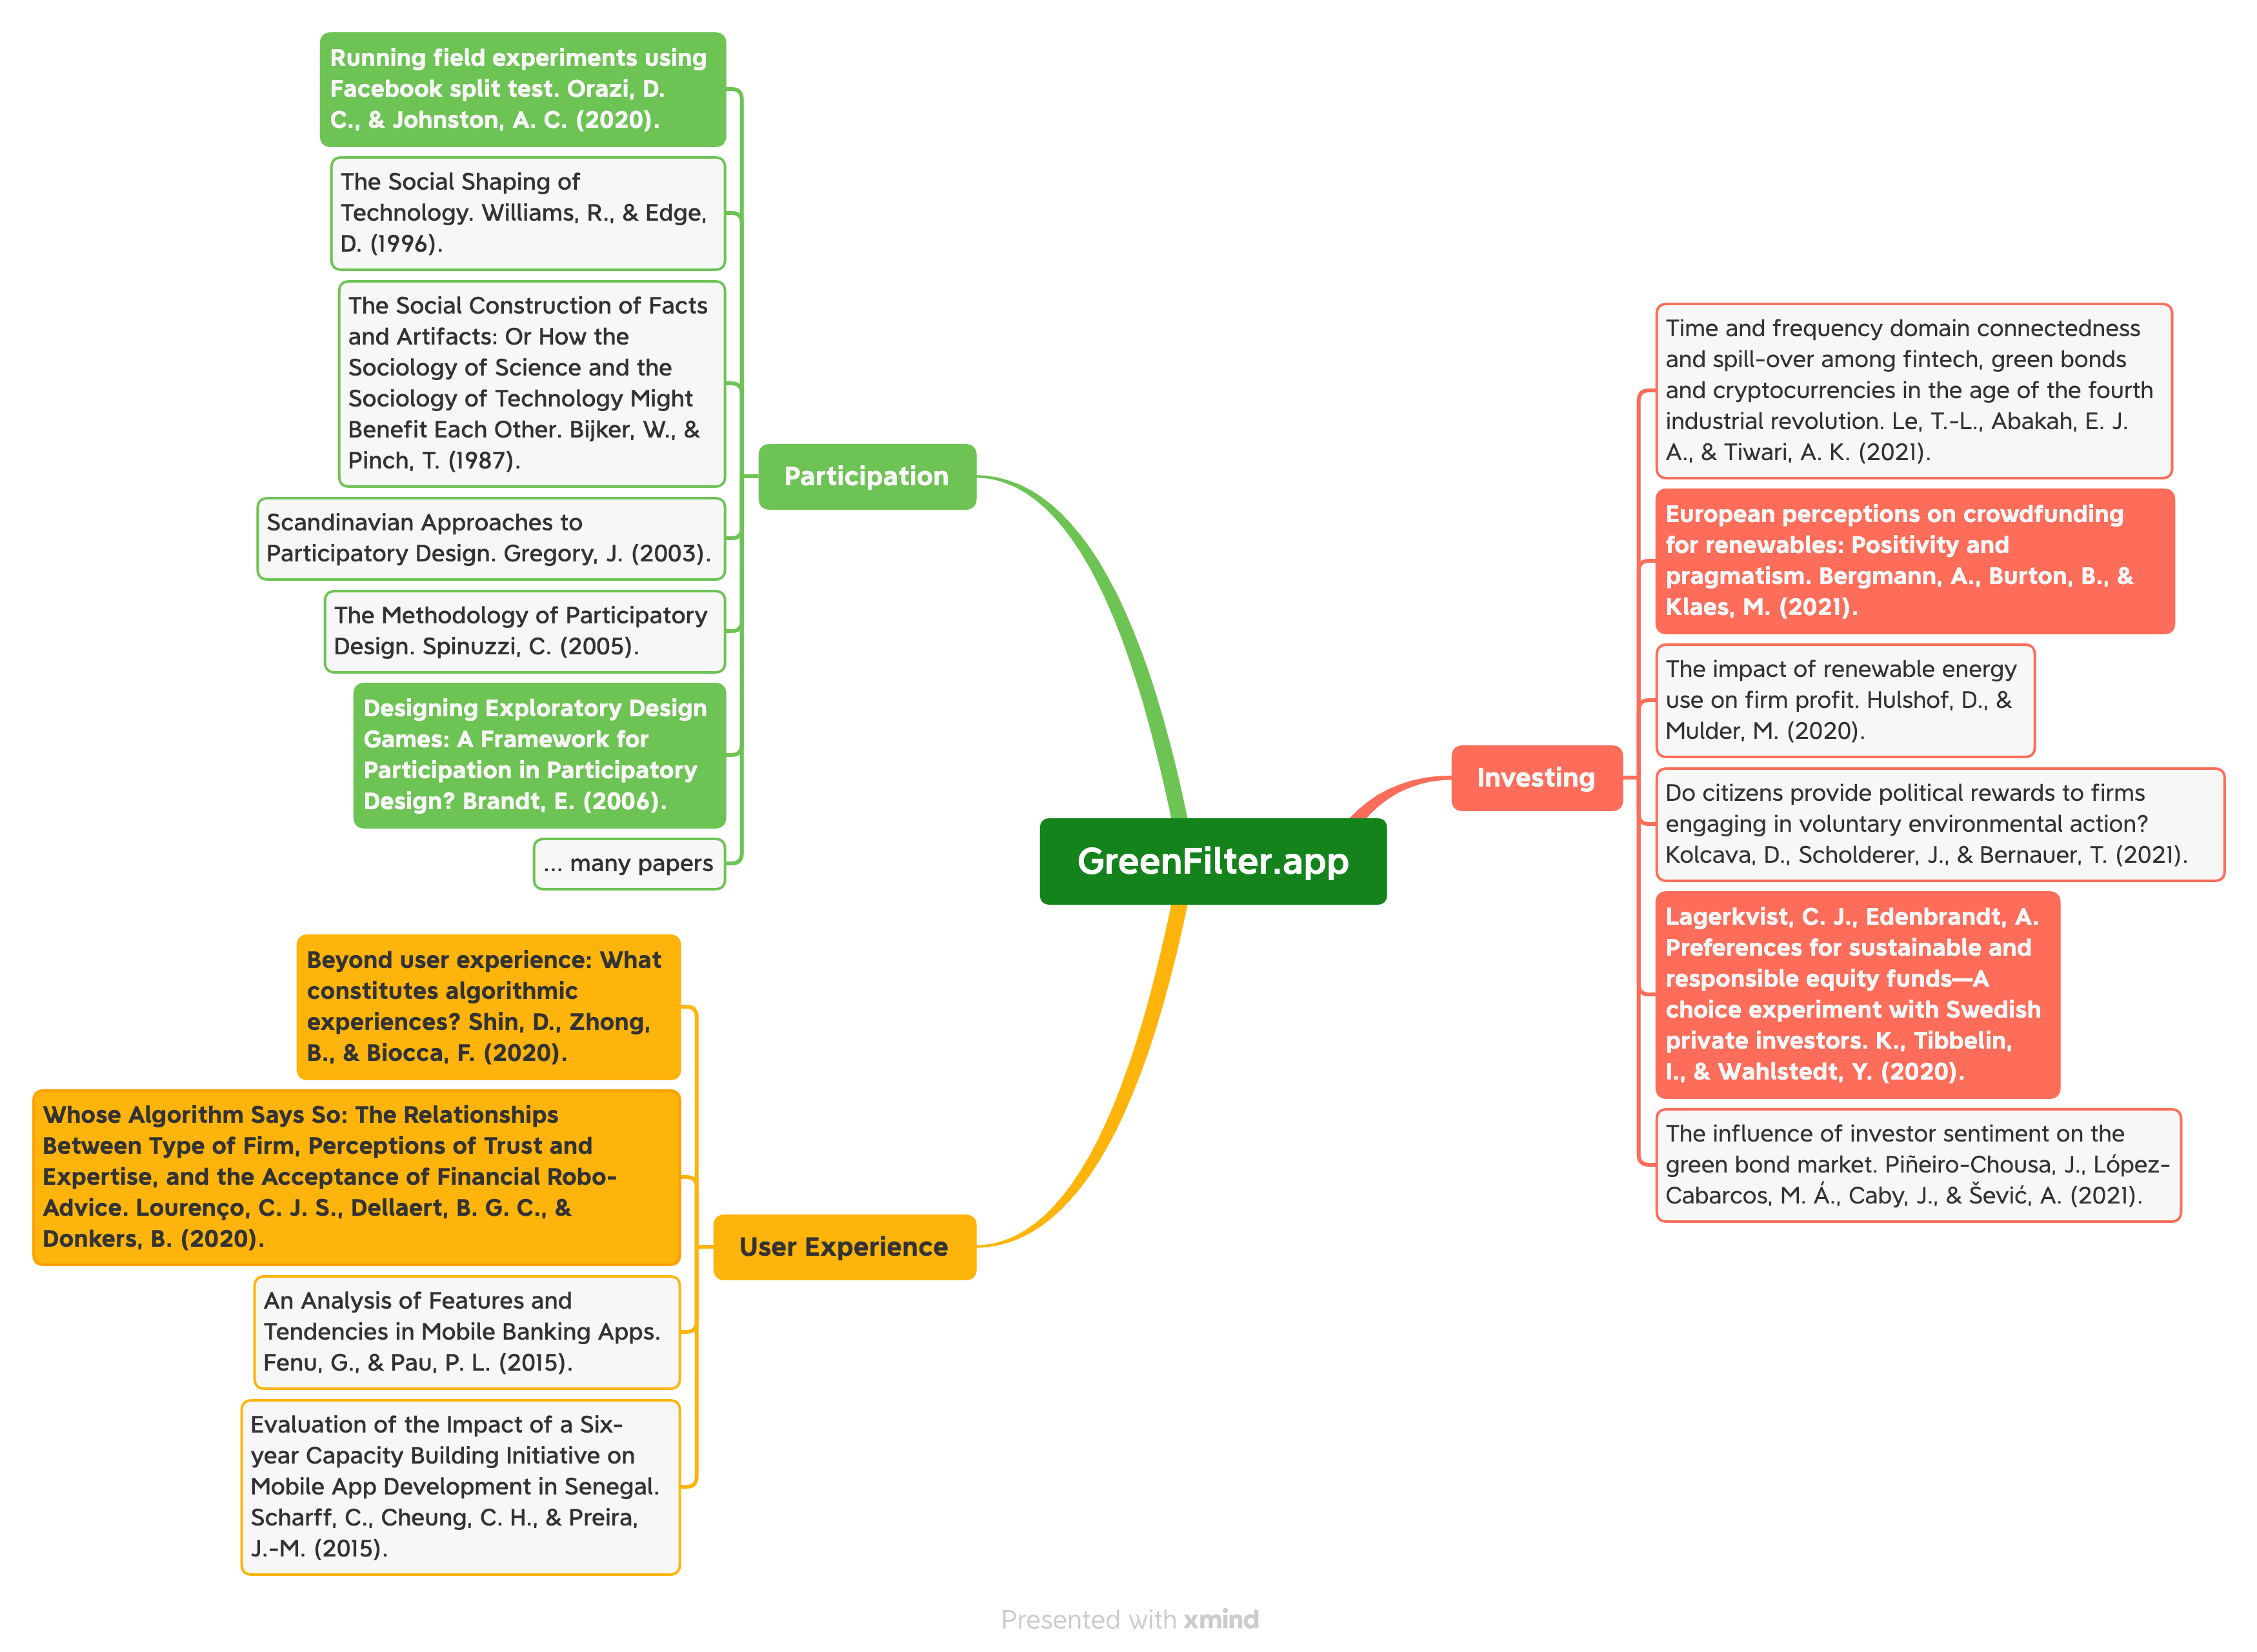
\includegraphics[width=1\linewidth,height=\textheight,keepaspectratio]{./images/literature/literature.png}

}

\caption{Example papers from the Literature Review}

\end{figure}%

\subsubsection{Sources}\label{sources}

There is currently no single platform that hosts all scientific journals
leading me to source scientific papers from

\begin{enumerate}
\def\labelenumi{\arabic{enumi}.}
\tightlist
\item
  ScienceDirect
\item
  Nature
\item
  The Lancet
\item
  Oxford Academic
\item
  Semantic Scholar
\item
  JSTor
\item
  Google search.
\end{enumerate}

\subsubsection{AI Use}\label{ai-use}

Statement of AI Usage in Research: I'm a long time AI-assistant user.

AI was used for:

\begin{enumerate}
\def\labelenumi{\arabic{enumi}.}
\tightlist
\item
  Search
\item
  Data comparison
\item
  Data science
\item
  Chart-building
\item
  Translation
\item
  Feedback
\item
  Editing
\item
  Spell-checking
\item
  Proofreading
\item
  Ranking citations' relevance to existing body of writing
\end{enumerate}

AI was \emph{NOT} used for writing.

A visualization of incremental changes (over a thousand Git commits) to
the thesis can be seen on the GitHub repository as well as in the
visualization below.

\newpage

\section{Young Adults and College
Students}\label{young-adults-and-college-students}

\subsection{Student Protests for Climate Justice: The World and
Taiwan}\label{student-protests-for-climate-justice-the-world-and-taiwan}

In August 2018, Swedish high-school student Greta Thunberg skipped class
to start a climate justice strike in front of the Swedish parliament
Riksdag. In 2019, Time magazine named Thunberg person of the year for
\emph{creating a global attitudinal shift} towards the environment
(Deutsche Welle, 2019). According to official statistics, 14 million
participants joined her \emph{Fridays for Future} strikes and the
movement expanded to over 7,500 cities around the world (Fridays For
Future, 2025). A survey 64 climate protesters from Norway, the UK, USA,
and Canada, found the climate-justice activists are non-homogeneous
group, displaying differing levels of factual knowledge about climate
change, a broad spectrum of emotions from anger to guilt and hope, with
diverse lifestyles, consumption habits, dietary shifts, and political
leanings (Martiskainen et al., 2020).

\begin{figure}[H]

{\centering 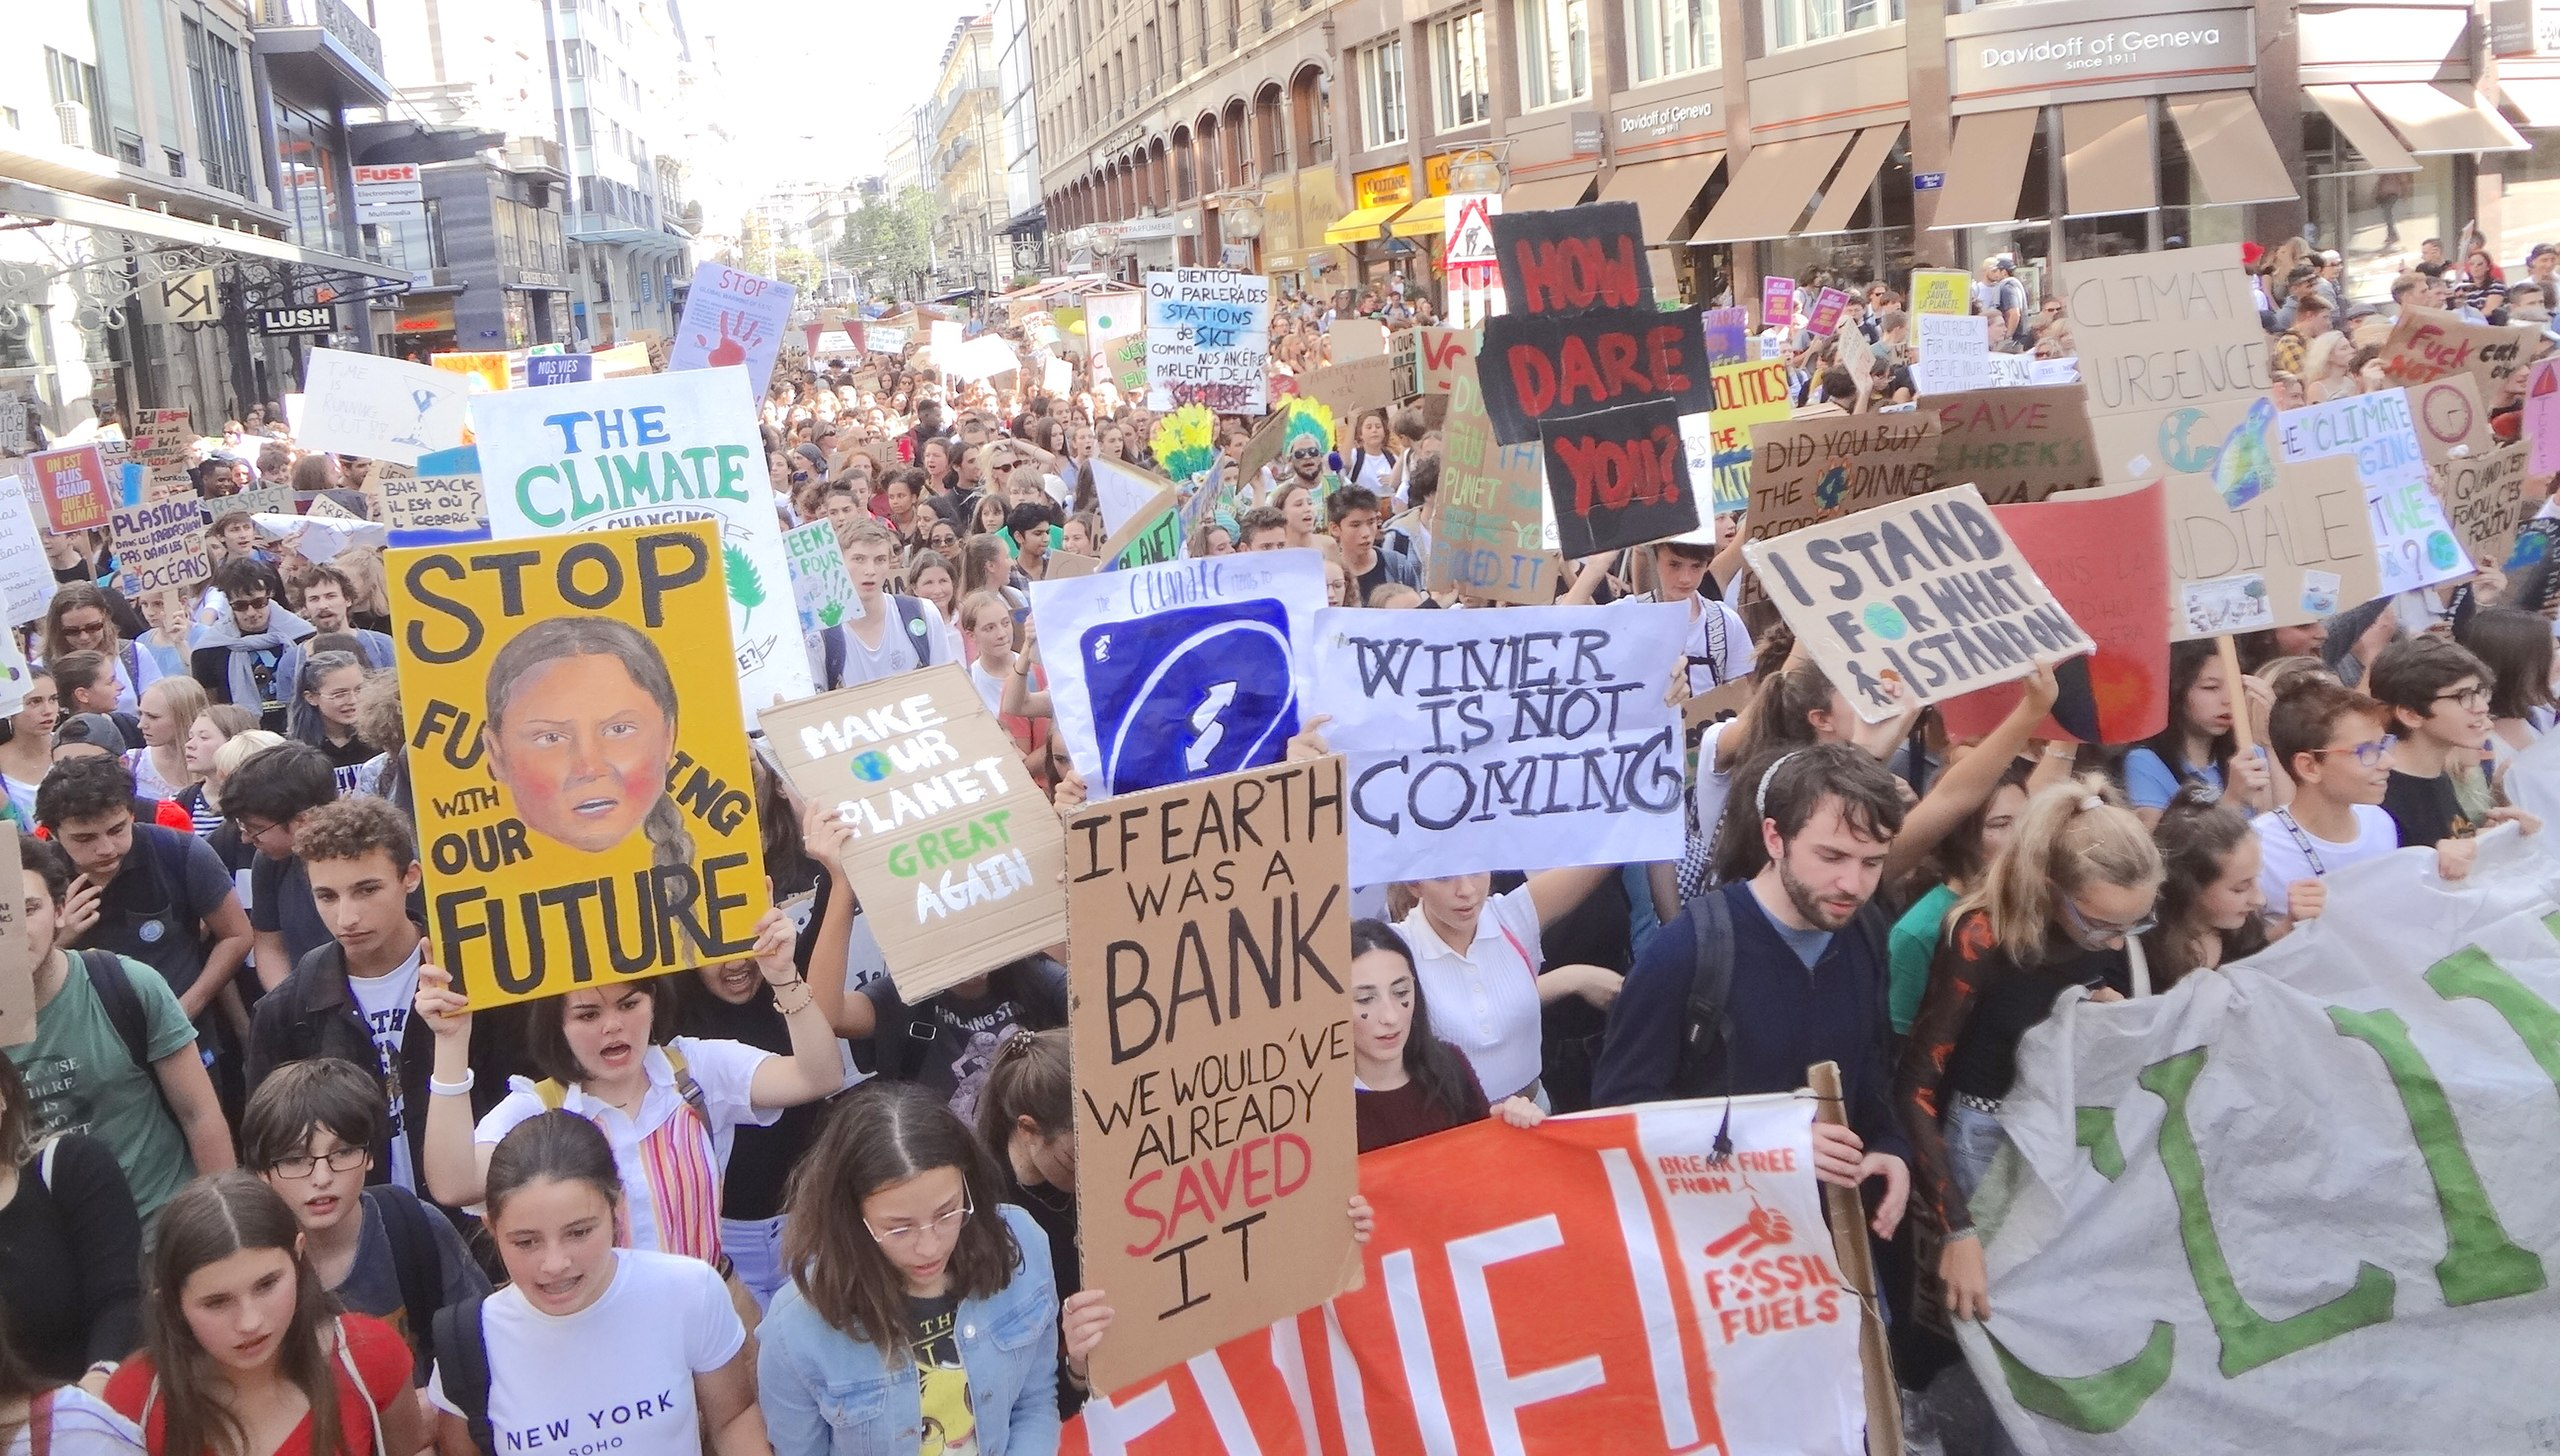
\includegraphics[width=1\linewidth,height=\textheight,keepaspectratio]{./images/college/geneve.jpg}

}

\caption{Climate protest in Geneva on September 27th, 2019 -- 1 year
after the start of Fridays for Future}

\end{figure}%

In Indonesia, which had large protests at the time, now 7 years later
activists are expressing disillusionment and frustration with the lack
of progress and upholding environmental promises. (Dwi Tamara, 2025)
reports on a survey of 382 Gen-Z respondents in 5 areas of Jakarta, with
99.5\% of the respondents having experienced extreme weather events
first-hand, highlighting how respondents were affected by
climate-related calamities, such as frequent flooding, which led to
students missing school days, - education which they are entitled to.
The Sharm El Sheikh climate policy implementation (UNFCCC, 2023b) text
refers to ``human right to a clean, healthy and sustainable
environment''. In Portugal, Estonia, and elsewhere young people have
moved on from strikes to actually taking legal action at the courts
suing companies for the environmental problems they have caused (Flor,
2024).

\begin{figure}[H]

{\centering 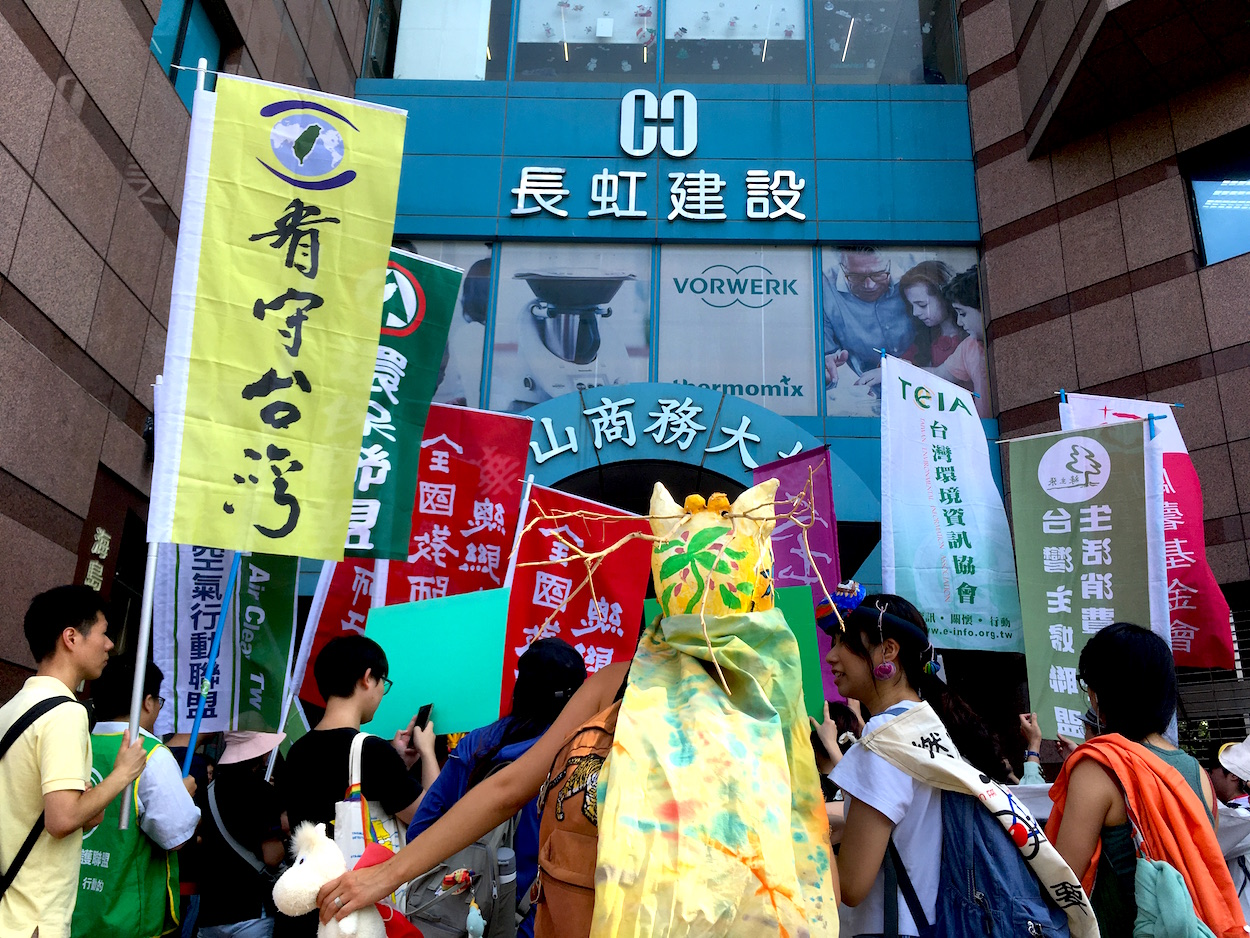
\includegraphics[width=1\linewidth,height=\textheight,keepaspectratio]{./images/college/taipei.jpg}

}

\caption{Climate protest in Taipei in May 2019 in front of the
Democratic Progressive Party (DPP) headquarters}

\end{figure}%

Meanwhile, as the climate-justice protests unfolded around the world, in
Taiwan, the Fridays for Future protests were very small in scale, with
no more than 100-200 people (Hioe, 2019). Meanwhile 2000 Taiwanese
students joined the initative by participating in environmental
activities without protesting (Dai, 2019). This could in part be
explained by Taiwanese culture being deeply influenced by Confucianism,
valuing stability, hierarchical relationships, academic excellence,
effort, and the role of education in achieving social status (R.-H. Xu,
2024). (H.-C. Chang, 2022) goes a step further to say that Taiwanese
youth are effectively unable to stage formal ``strikes'' due to
intersecting cultural constraints: obsession with academic performance,
low awareness of legal strike rights, and parental intervention --- so
they instead reframe actions as campus ``climate actions,'' exercising
agency within those limits. In addition, both Confucianism and Daoism,
the prevalent belief systems in Taiwan, affect education to be
\emph{teacher-centered}, where traditionally the role of students is to
listen and absorb knowledge; in today's society, there's space to open
opportunities for revisiting \emph{dialogue-based} education, where
students would be encouraged to take a more active role and gain
ownership of their education (C.-C. Chang et al., 2023).

\subsection{Taiwanese Educational System in
Numbers}\label{taiwanese-educational-system-in-numbers}

Taiwan has approximately 2 million young adults (Gen-Z, 18-26), and 73\%
percent of them are students attending tertiary education as of 2023,
with a slow increase of enrollment over the past decade (Ministry of
Education of Taiwan, 2024b).

\begin{figure}

\centering{

\pandocbounded{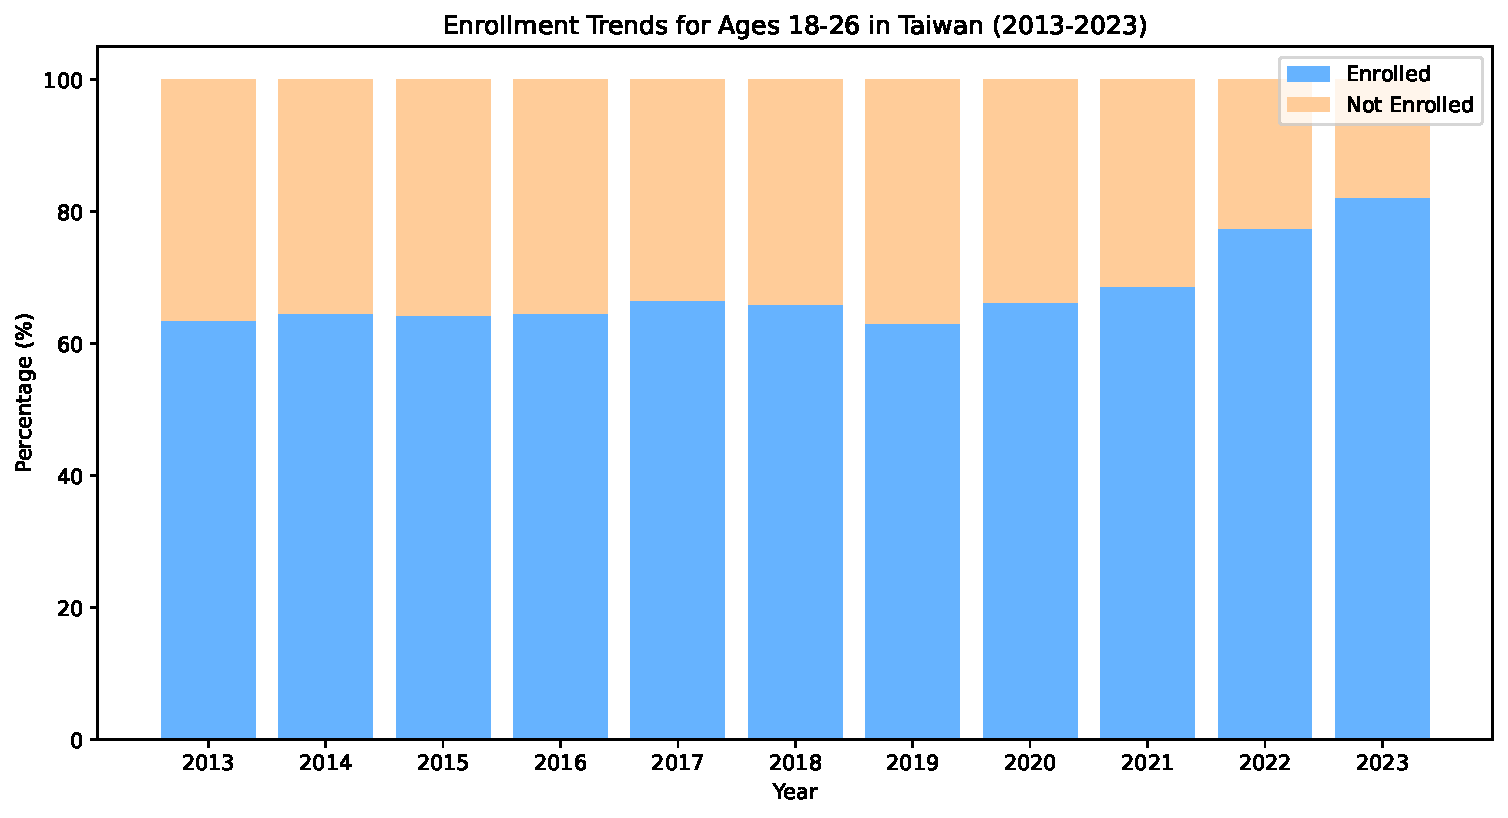
\includegraphics[keepaspectratio]{_thesis_files/figure-pdf/fig-tw-high-ed-enrollment-output-1.pdf}}

}

\caption[Enrollment in Taiwanese Higher
Education]{\label{fig-tw-high-ed-enrollment}Enrollment in Taiwanese
Higher Education}

\end{figure}%

As of 2024, Taiwan has a total of 148 universities, colleges, and junior
colleges (Ministry of Education of Taiwan, 2024c). Education funding is
4.26\% of Taiwan's GDP in 2023-24 and has been on a decline for a decade
(Ministry of Education of Taiwan, 2024a). Taiwan has an aging population
and declining birth rates have forced several schools to close down
(Davidson \& Chi-hui, 2024; Goh et al., 2023).

\begin{figure}

\centering{

\pandocbounded{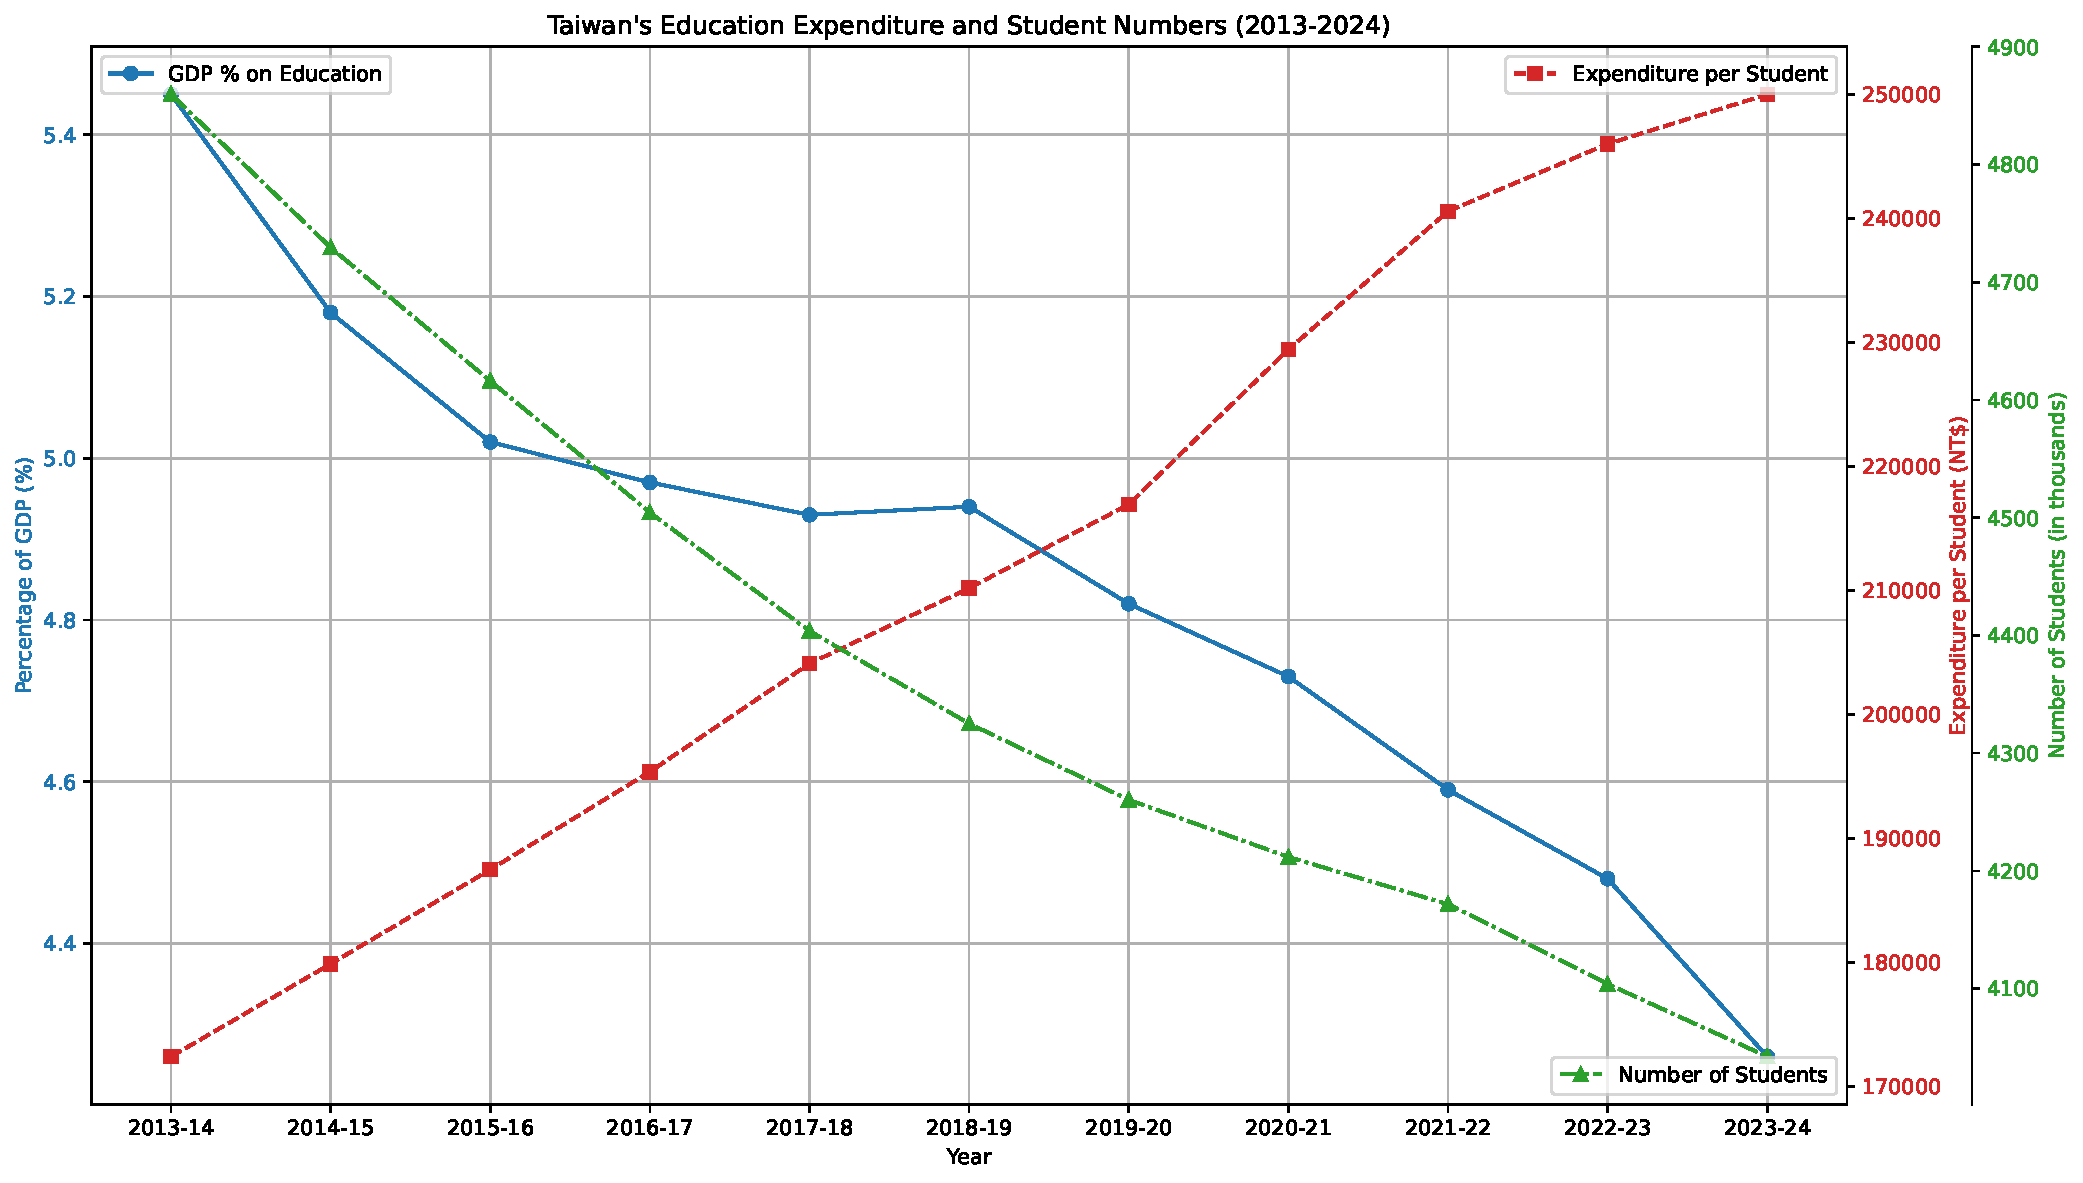
\includegraphics[keepaspectratio]{_thesis_files/figure-pdf/fig-tw-high-ed-funding-output-1.pdf}}

}

\caption[Funding for Taiwanese Higher
Education]{\label{fig-tw-high-ed-funding}Funding for Taiwanese Higher
Education}

\end{figure}%

While the overall number of students is declining, the share of
international students is increasing.

\begin{figure}

\centering{

\pandocbounded{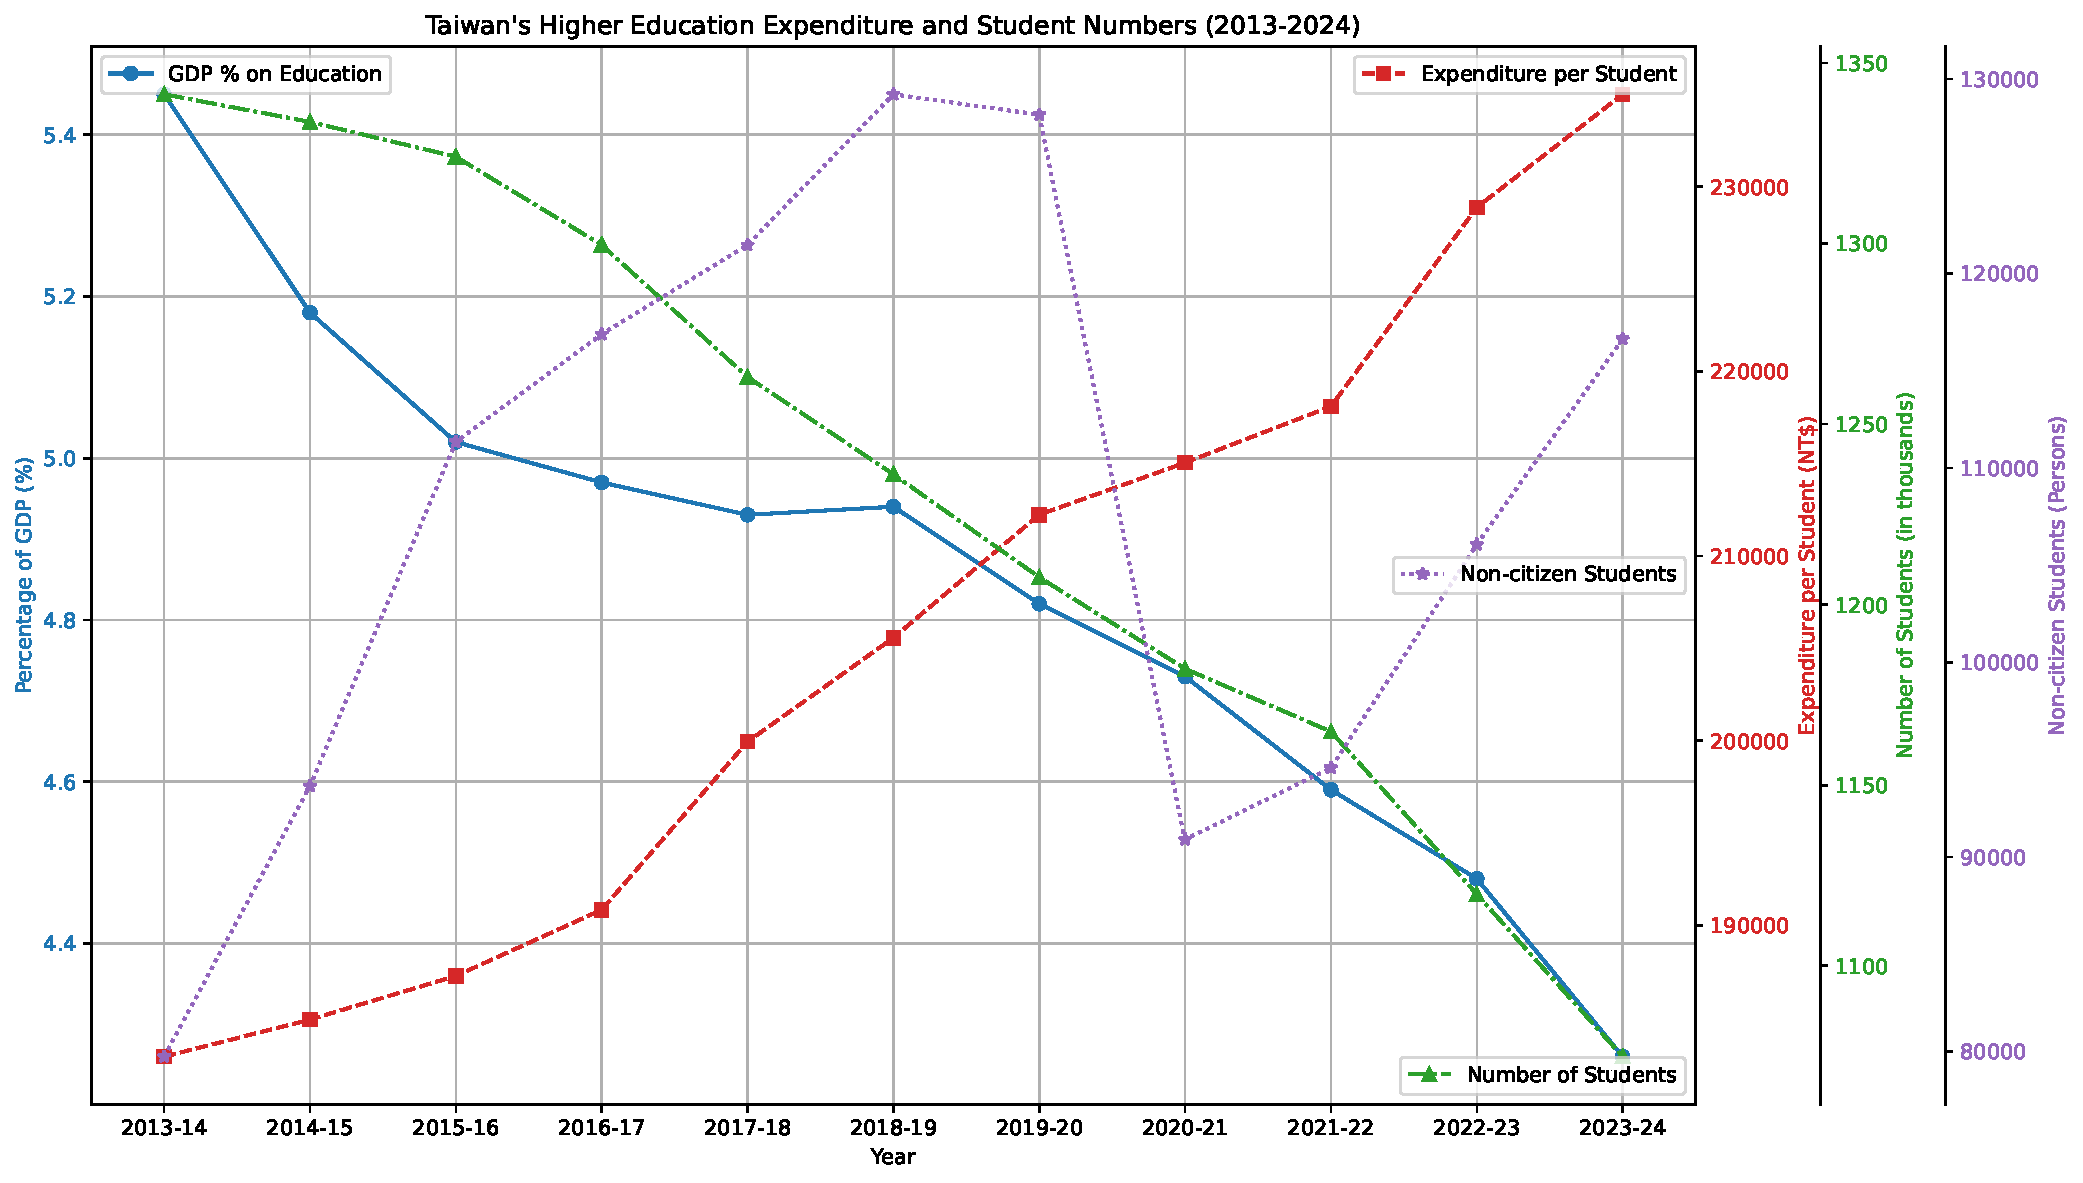
\includegraphics[keepaspectratio]{_thesis_files/figure-pdf/fig-tw-high-ed-output-1.pdf}}

}

\caption[Demographics of Taiwanese Higher
Education]{\label{fig-tw-high-ed}Demographics of Taiwanese Higher
Education}

\end{figure}%

\subsection{Designing for College Students: Developing
Personas}\label{designing-for-college-students-developing-personas}

Students in the Generation-Z age bracket (abbreviated as Gen-Z or
Zoomers) are born between 1997 and 2012 (Branka Vuleta, 2023). High
levels of technology adoption worldwide (Deyan Georgiev, 2023a). Over
98\% of Gen-Z owns a smartphone while only 80\% of the general world
population does (BankMyCell, 2022; Global Web Index, 2017).

Designing for College Students: Developing Personas. User research makes
extensive use of user \emph{personas} to represent a group of people
with similar attributes. Designers use personas to \emph{articulate
assumptions,} which, if used well, is useful for \emph{user-centered
design}, to create better products. Personas help to reflect on what
kind of \emph{biases} might exist in the design. Within the larger
cohort of college students several different personas could be defined,
for example grouping people by interests, knowledge, habits, levels of
anxiety, and other attributes. Humans have a long list of cognitive
biases, which a good design should take into account.

Many general observations can be made, however to create meaningful
personas, these should be backed up with data. Students ride bicycles
and scooters. Many circular economy service such as YouBike and
transport sharing platforms like Uber are available in Taiwan. Many
students live in dorms and shared housing, meaning their impact per
square meter is low.

\subsection{Taiwanese Youth in Global Context: Sustainability Attitudes
From Eco-Friendly Diet to Climate
Action}\label{taiwanese-youth-in-global-context-sustainability-attitudes-from-eco-friendly-diet-to-climate-action}

Addressing the Research Gap When it Comes to Taiwanese College Students.
There's lack of scientific research when it comes to Taiwanese college
students, not only in English or other foreign languages, but also in
Chinese. Much of the research in Taiwan focuses on younger students,
particularly those in primary and secondary schools. With regards to
issues related to college students and sustainability, even less
research is available. My project hopes to shed some light to how
Taiwanese college students relate to sustainability.

(Kuo-Hua Chen, 2019) compares Taiwan to other countries in terms of
\emph{Postmaterialist Index Comparison}, noting Taiwanese society is
materialistic.

\begin{figure}

\centering{

\pandocbounded{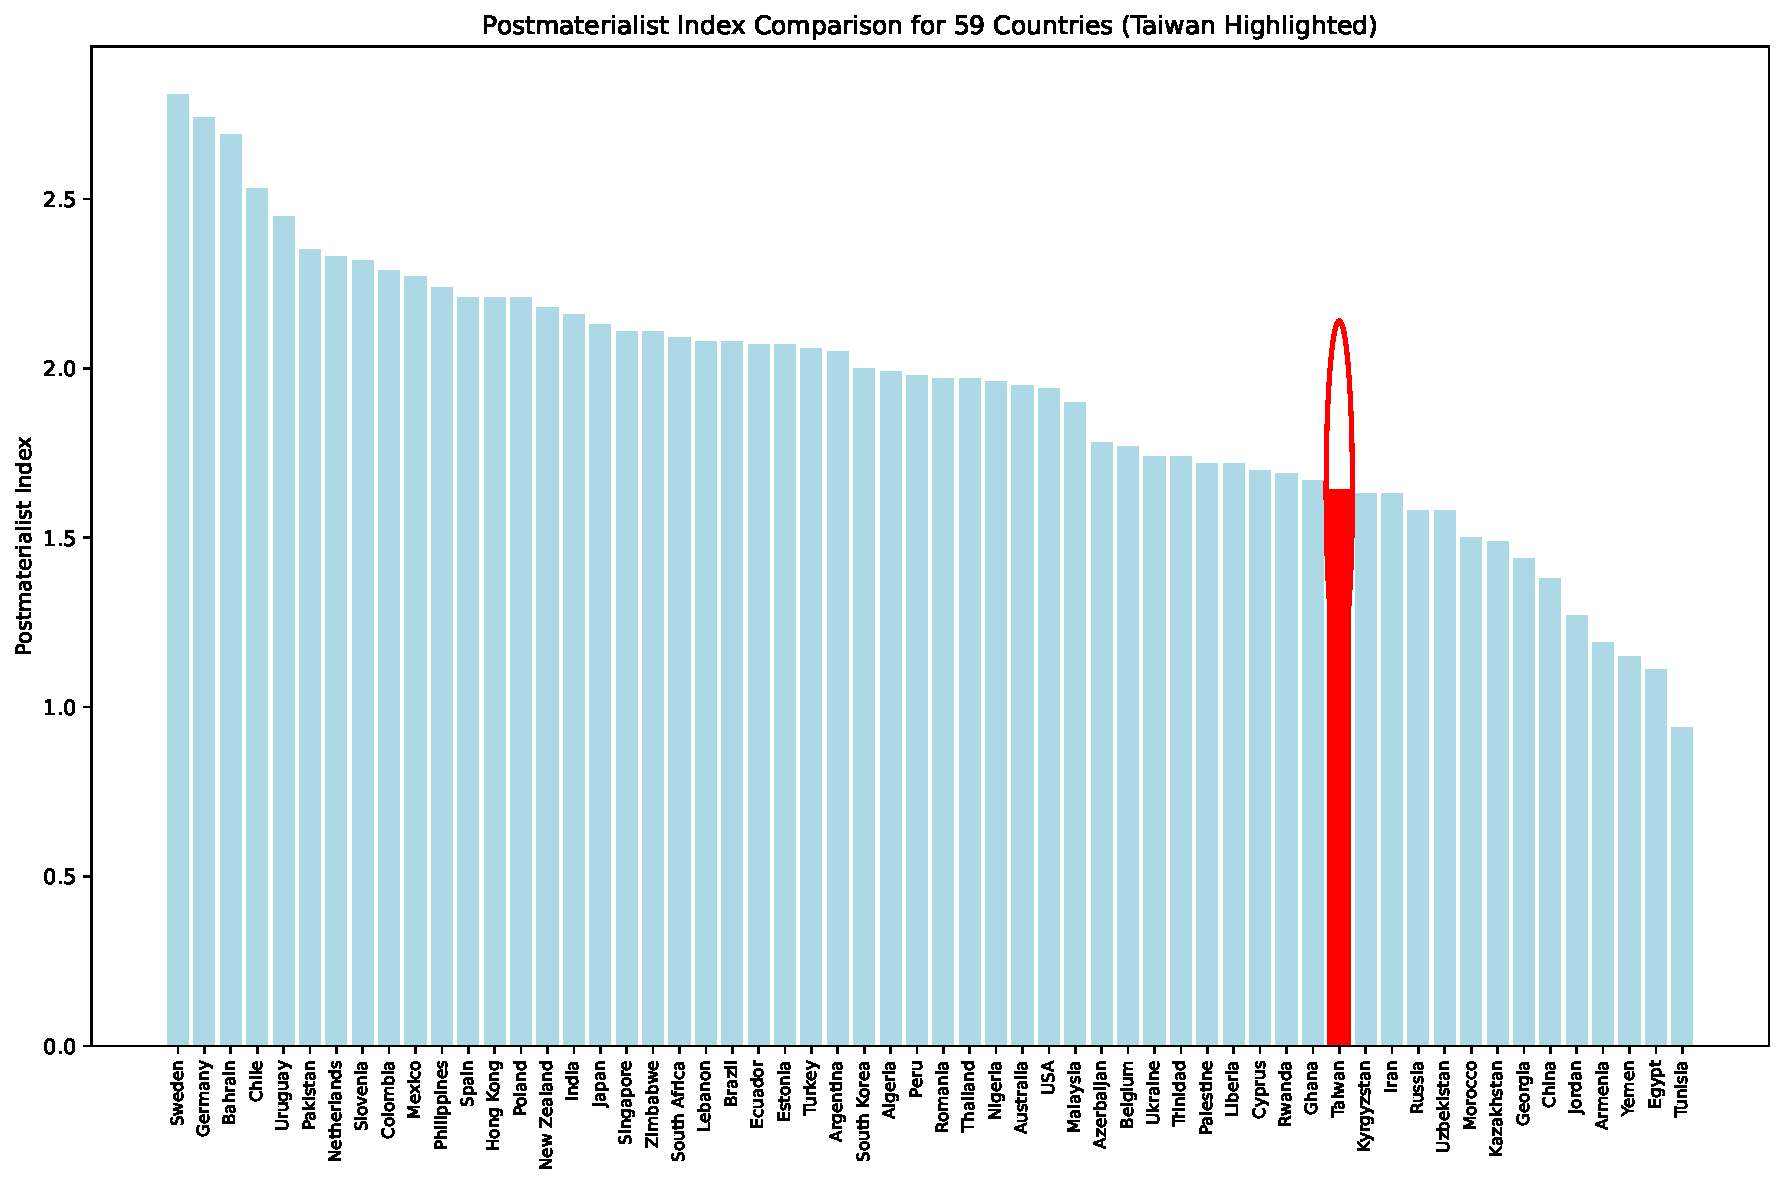
\includegraphics[keepaspectratio]{_thesis_files/figure-pdf/fig-postmat-index-output-1.pdf}}

}

\caption[Postmaterialist Index (Taiwan
Highlighted)]{\label{fig-postmat-index}Postmaterialist Index across 59
countries (Taiwan highlighted)}

\end{figure}%

World Values Survey

\begin{figure}

\centering{

\pandocbounded{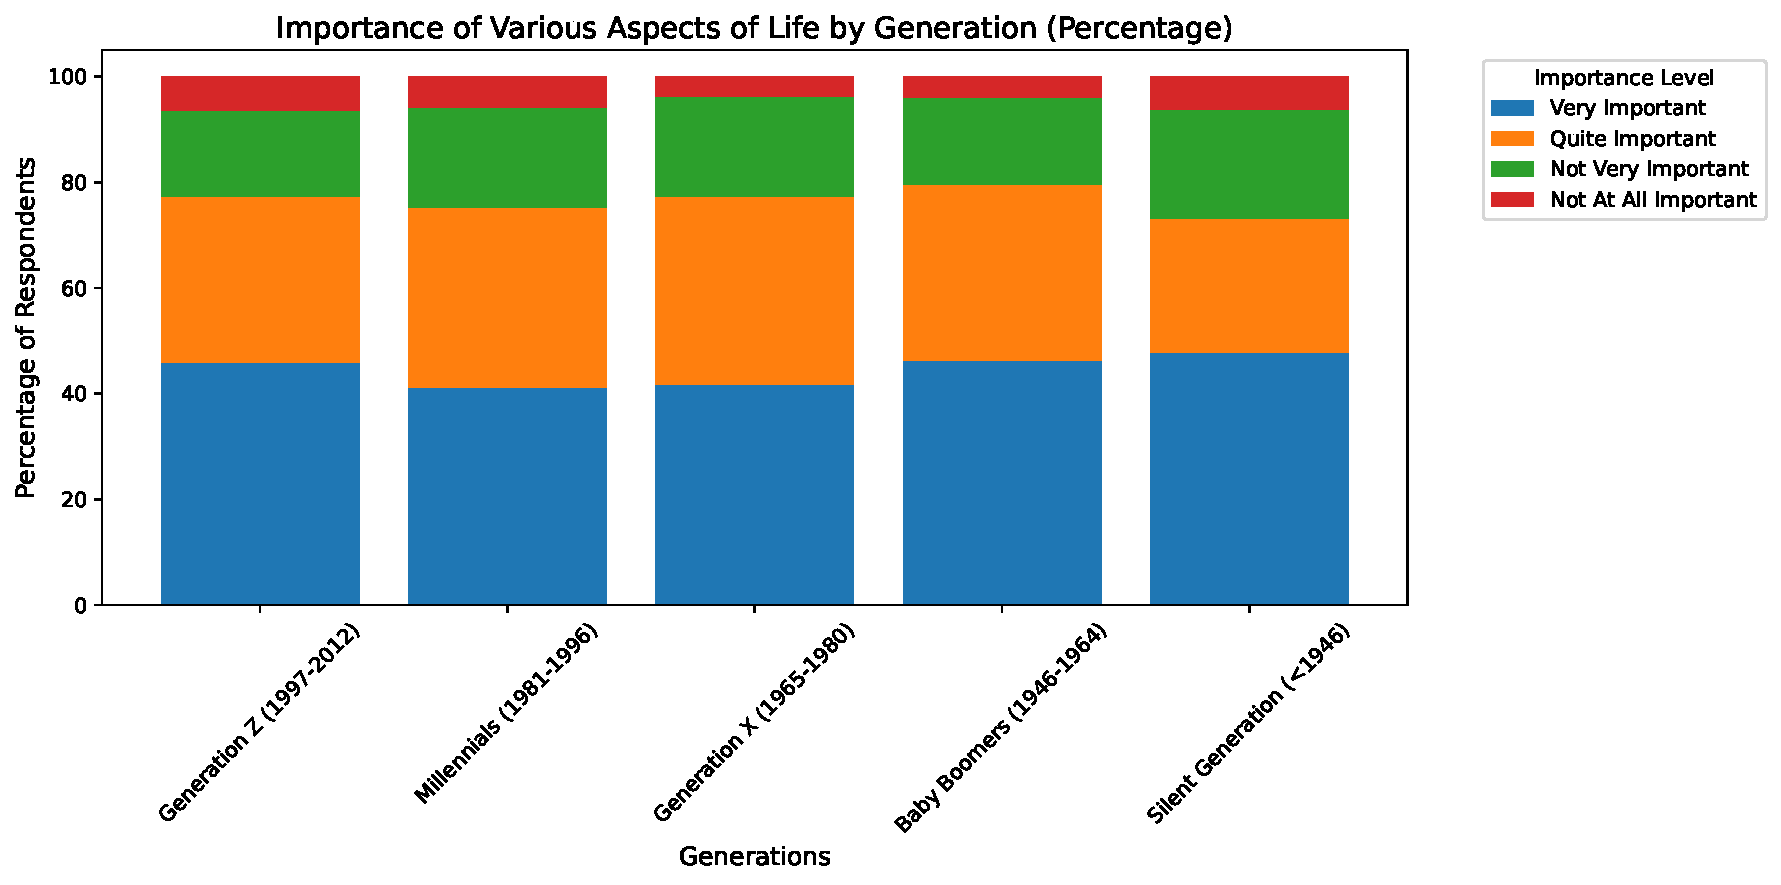
\includegraphics[keepaspectratio]{_thesis_files/figure-pdf/fig-world-values-output-1.pdf}}

}

\caption[World Values Survey]{\label{fig-world-values}World Values
Survey}

\end{figure}%

(Franzen \& Bahr, 2024) measures \emph{``mean environmental concern''}
to look at decade-level changes in societal environmental attitudes
across countries. Taiwan's general attitudes have stayed almost the same
(slight increase). The UK has had the largest jump in concern.
Curiously, South Korea has had a slight decrease in concern. Slovakia
and Russia were not very concerned with the environment a decade ago and
are even less concerned now.

A large, global-scale study by (Anthony Leiserowitz et al., 2022)
administered on Meta's Facebook (n = 108946) reported people in Spain
(65\%), Sweden (61\%), and Taiwan (60\%) believe \emph{``climate change
is mostly caused by human activities''}.

\begin{figure}

\centering{

\pandocbounded{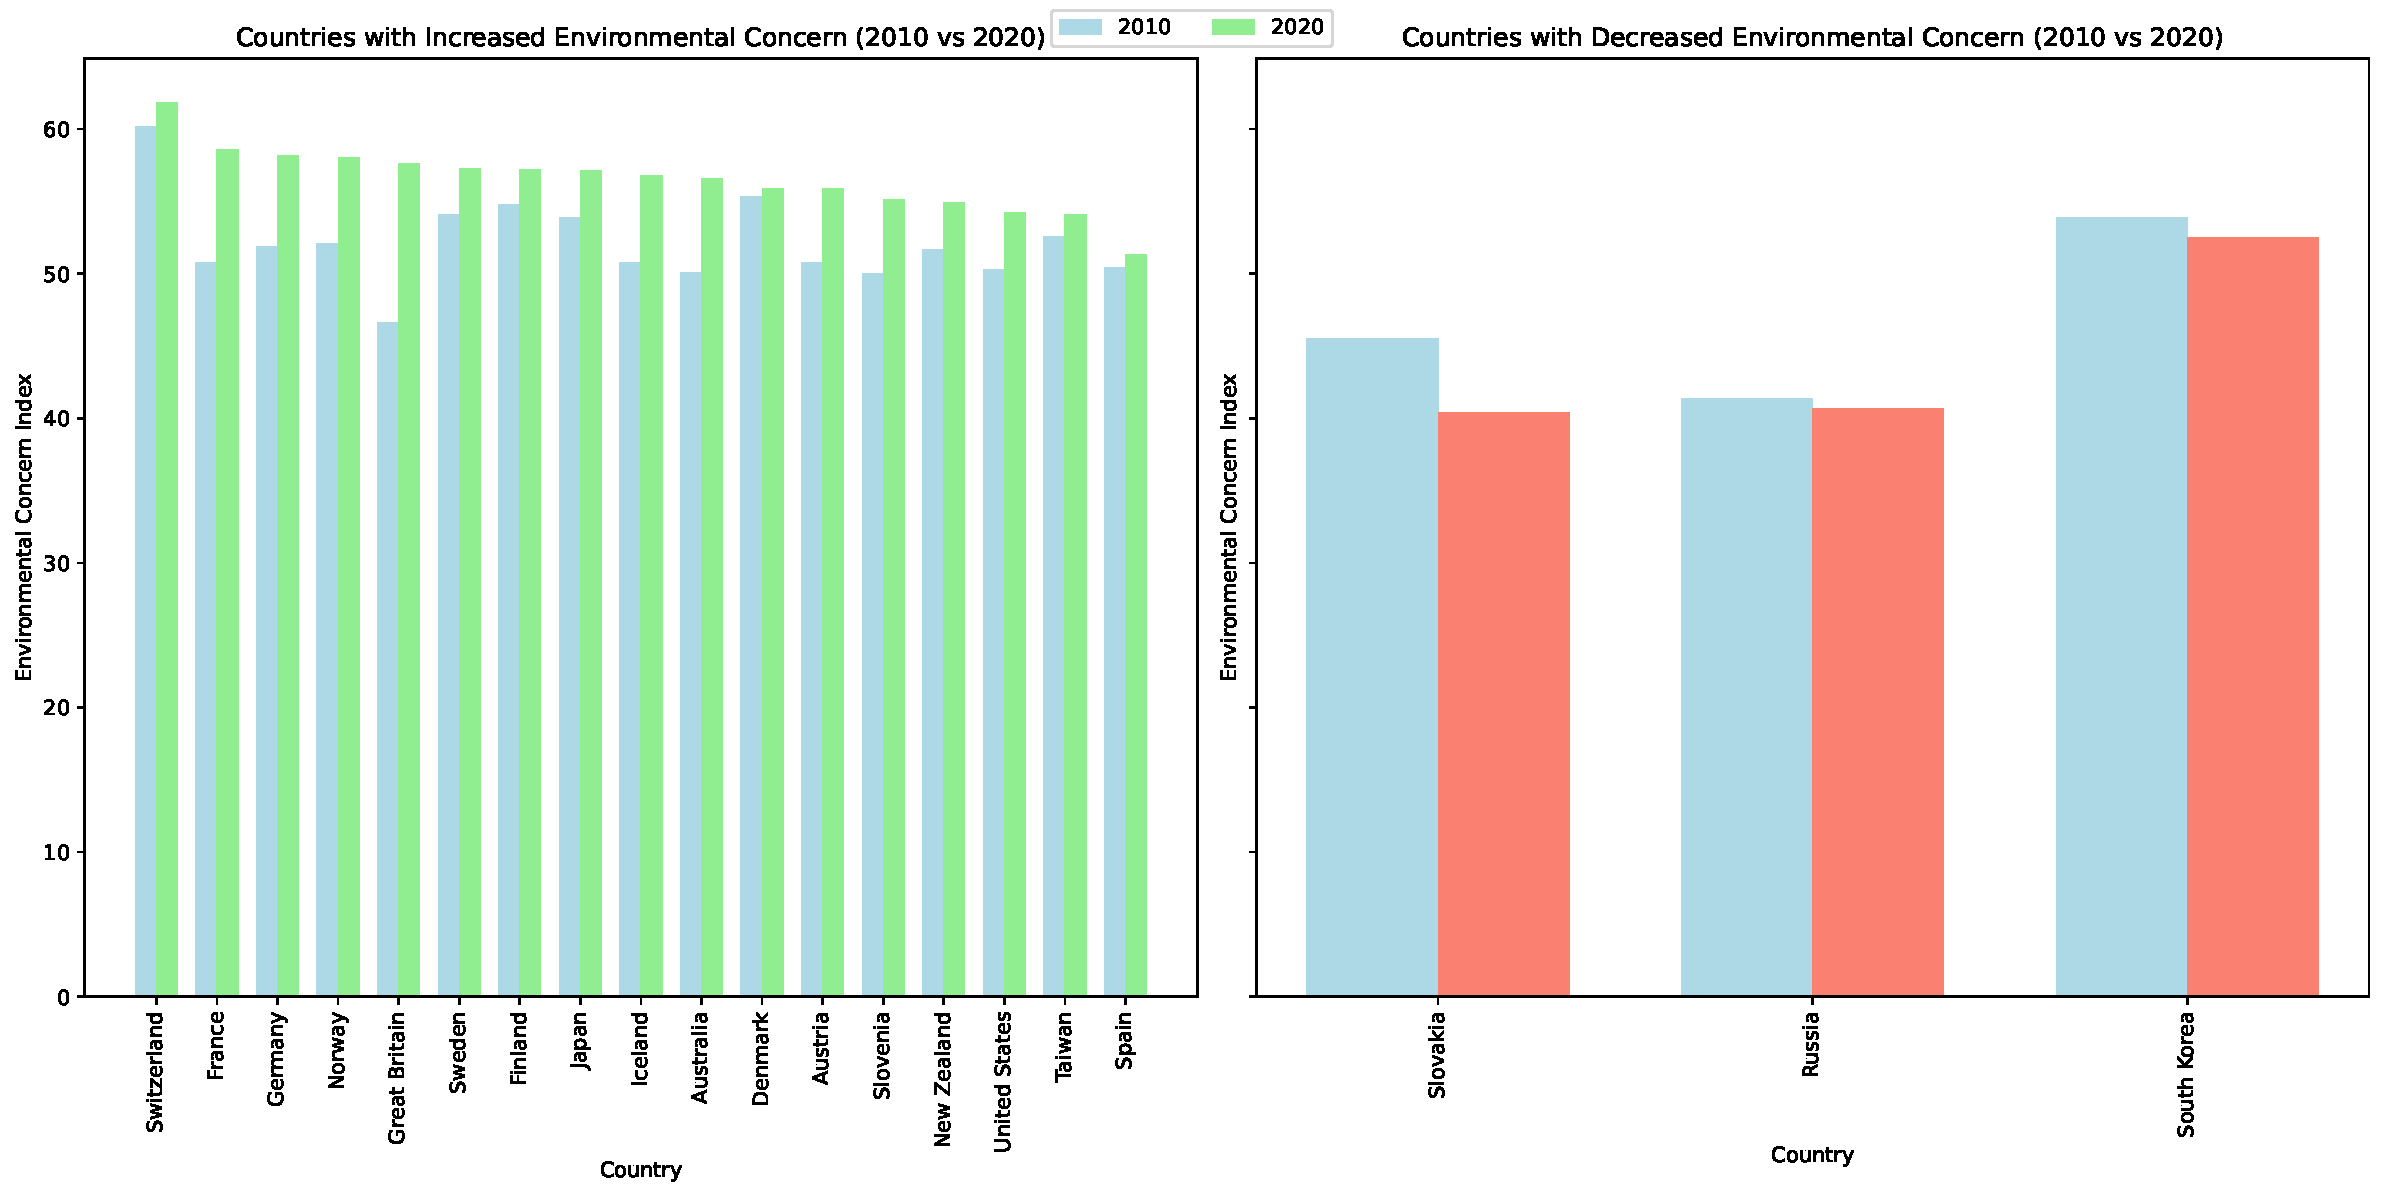
\includegraphics[keepaspectratio]{_thesis_files/figure-pdf/fig-global-climate-attitudes-output-1.pdf}}

}

\caption[Global Attitudes Towards Climate
Change]{\label{fig-global-climate-attitudes}Global Attitudes Towards
Climate Change}

\end{figure}%

The largest study to date, conducted by the United Nations across 50
countries, surveying 1.2 million people, distributed through mobile game
ads, showed the majority of people agreeing climate change is an
``emergency'' (UNDP, 2021).

\def\pandoctableshortcapt{UN Survey: 1.2 Million Responses to
\emph{Climate Change Is An Emergency}}

\begin{longtable}[]{@{}lll@{}}
\caption[UN Survey: 1.2 Million Responses to *Climate Change Is An
Emergency*]{1.2 million UN survey responses to the statement ``Climate
change is an emergency''.}\tabularnewline
\toprule\noalign{}
\endfirsthead
\endhead
\bottomrule\noalign{}
\endlastfoot
Age Group & Agree & Neutral or Disagree \\
18-35 & 65\% & 35\% \\
36-59 & 66\% & 34\% \\
Over 69 & 58\% & 42\% \\
\end{longtable}

\let\pandoctableshortcapt\relax

At the pre-university level, Taiwanese government has been promoting
environmental education through a green school network; however surveys
at middle school and high school level suggest there is no impact on
\emph{sustainability consciousness} among students in comparison with
regular schools (Olsson et al., 2019). Rather, Taiwanese students are
influenced towards environmental action by \emph{group consciousness}
(T.-Y. Yu et al., 2017). In contrast,(陳珮英, 2003) reports \emph{good
knowledge of sustainable development} topics among \emph{junior high
school students} in Da-an District, Taipei City (n =596). (林建輝.,
2009) similarly reports a positive attitude and good knowledge of
environmental sustainable development among senior \emph{high school
students} towards in Taipei City (n = 328). Several Taiwanese studies
also focus on the physical environment of school campuses, for example
the sustainability of elementary school campuses (潘智謙 \& Pan, 2006).
Elementary-school teachers in Taichung (n = 536), have positive
attitudes towards environmental education are positive, proactive and
demonstrate high awareness; they have participated in many
sustainability-related workshops (Liao et al., 2022).

At the university level, (C.-L. Chen \& Tsai, 2016) reports a
\emph{positive attitude yet moderate knowledge} about \emph{ocean
sustainability} among Taiwanese college students (n = 825). (C.-H. Liu
et al., 2023) studied sustainability behavior of Taiwanese University
students, reporting the COVID-19 pandemic, in addition to prevalence of
health issues, also spurred more attention on environmental topics. In a
similar vein, the devastating nuclear disaster in Fukushima, Japan,
after 2011 earthquake, had an effect on Taiwanese energy and
sustainability education (姚 \& 侯, 2011). Taiwanese government launched
the Sustainable Council in 1997 to promote of environmental and
sustainable development; a survey of university-level teachers (n = 100)
in central Taiwan (Taichung, Changhua, and Yunlin) shows a positive
attitude toward environmental sustainability among teachers however
implementation of environmental sustainability practices is from low to
medium range (林美惠. \& 莊, 2015). Taiwanese government has also
launched funding for University Social Responsibility (USR) programs to
train college students in social innovation and local revitalization (D.
Chen \& Chou, 2023; W.-H. Liu et al., 2022). In general, it could be
concluded, Taiwanese students and teachers at all levels of education
have a positive attitude towards sustainability (Note: which is not a
very actionable finding).

Comparing college students' education for sustainable development (ESD)
in Taiwan (n = 617) and Sweden (n = 583) found Sweden has a long history
in environmental education while in Taiwan environment became a focus
area with the 1998 educational reform (Berglund et al., 2020).

\begin{figure}

\centering{

\pandocbounded{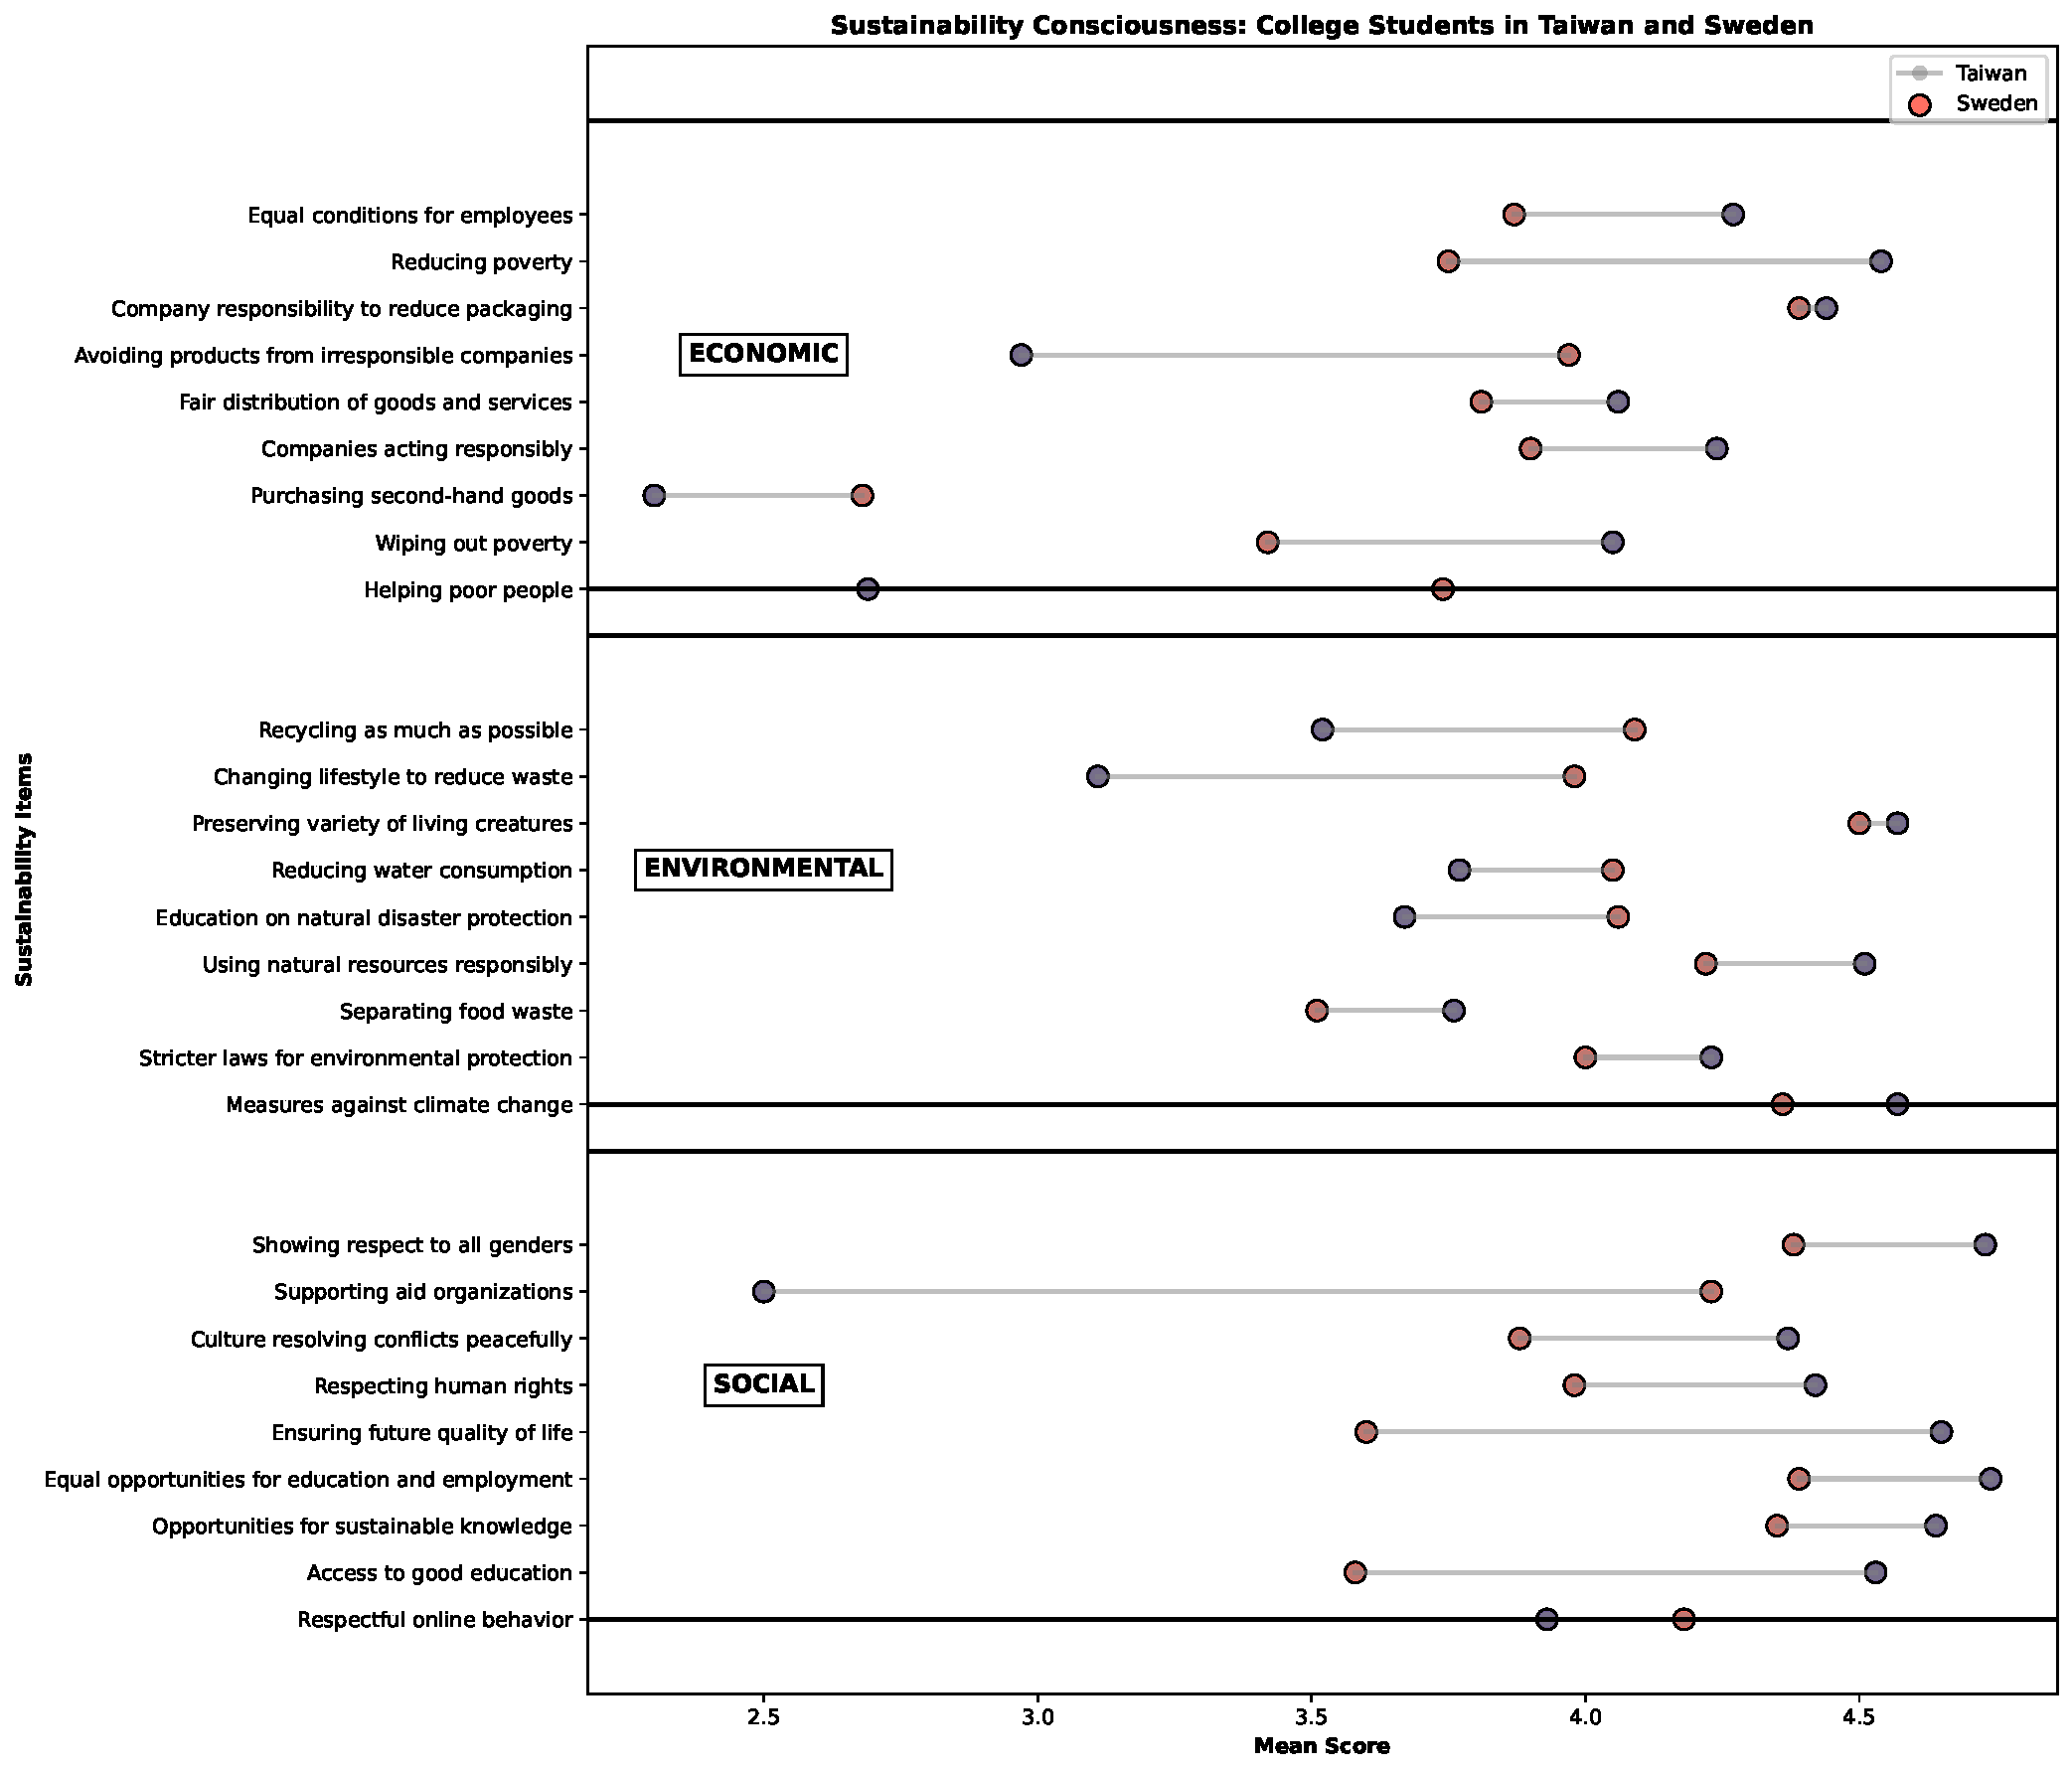
\includegraphics[keepaspectratio]{_thesis_files/figure-pdf/fig-tw-swe-output-1.pdf}}

}

\caption[College Students' Sustainability Education: Taiwan vs
Sweden]{\label{fig-tw-swe}Comparing college students' education for
sustainable development in Taiwan and Sweden}

\end{figure}%

An older study in 5 university in Taipei and Taichung (n = 255) found
78.04\% of respondents consumed beef in the month prior and were
concerned with food safety, freshness, and quality (J. L. Hsu et al.,
2014). (Thiagarajah \& Kay, 2017) reports a general observation in their
abstract (I was unable to access the full study) that most college
students in all observed countries including Taiwan (n = 534) regarded
``\emph{plant-based diets to have health benefits''}. A focus on a
healthy and sustainable diet is important, as the prevalent trend among
Taiwanese Gen-Z, is increasing obesity, with the latest data available
from 2020; the newest, 3rd wave national health survey results are still
pending (Chiu et al., 2022; 台灣營養師, 2022; 彭巧珍 et al., 2023).
Recent nationwide data show that 70\% of common bottled drinks (n = 341)
marketed to youth in Taiwan exceed the warning threshold for
\emph{``high sugar''} (\textgreater{} 5 g/100 mL), and a single serving
of 42\% of the drinks (\textgreater{} 25 g sugar per bottle) contained
the entire daily sugar limit prescribed by the World Health Organization
(WHO) (Yen et al., 2022).

Internationally, there is extensive research on the attitudes of college
students towards climate change. (American Press Institute, 2022)
reports only 37\% percent of U.S. Gen-Z and Millenials follow news
related to environmental issues. (S. E. O. Schwartz et al., 2022)
reports some adult U.S. students in a small study (18-35, n = 284)
express feelings of insignificance of their actions to achieve any
meaningful impact. (Thomaes et al., 2023) reports U.S. adolescents don't
find sustainability relevant to their daily life. (Ross et al., 2016)
says most people in the U.S. don't act on climate change. ``Action on
climate change has been compromised by uncertainty, aspects of human
psychology''.

(Credit Suisse, 2022) suggests young consumers are more eco-friendly and
drive the speed of change. Yet the Economist has ran a few anonymous
articles calling gen-z green ideals into question ({``How {Gen Z} and
Millennials Spend Their Money,''} 2023; The Economist, 2023). (Wood,
2022) suggests in the U.S. Gen-Z is willing to pay 10\% more for
ethically goods, spend 24\% more on sustainable products than Generation
X and 75\% of Gen Z would prioritize sustainability over brand loyalty.
Meanwhile Gen-Z in the U.S. are heavy users of online fashion shopping,
Chinese cheap online store Shein overtakes Amazon as the most downloaded
shopping app, while clothes resale apps such as Depop and ThredUp grow
in popularity (Alex Reice, 2021). It worth noting, Taiwan is also a
growing market for luxury brands (Karatzas et al., 2019).

(Manchanda et al., 2023) survey (n = 726) administered at shopping malls
in New Delhi, India, found similar levels of sustainability
consciousness between Millenial (n = 206) and Generation-Z (n = 360) age
groups; people with high level of materialism were found to be less
sustainability-conscious; the effect of mindfulness on sustainability
was found to be stronger among females than males, supporting the
hypothesis of the moderating effect of gender.

\subsection{The Experience of Climate Change and Pollution Levels in
Taiwan}\label{the-experience-of-climate-change-and-pollution-levels-in-taiwan}

Taiwan's recent climate challenges with over 4 decades of droughts,
rising air temperatures, and shifting rainfall patterns, have impacted
both water security and the performance of its vital semiconductor
manufacturing industry \hspace{0pt}(Vo \& Liou, 2024). Offshore, marine
heatwaves, ocean acidification, and elevated sea surface temperatures
are intensifying coral bleaching around Taiwan (P.-C. Hsu et al., 2024).
The oceans are crucial for Taiwan to capture carbon emissions. Around
33\% of Taiwanese CO\textsubscript{2}eq emissions is captured by the
marine carbon sink, while the effect of forests in Taiwan needs further
study (Hung et al., 2024).

Similarly to how Northern Europe, including Estonia, is affected by the
Gulf Stream, making the climate warmer, Taiwan is affected by the
Kuroshio (黑潮) warm current of the Pacific Ocean, which helps regulate
the climate and marine ecosystem of the region. The strength and
trajectory of the Kuroshio is influenced by Rossby planetary waves,
driven by the Earth's rotation are crucial to keeping the atmosphere in
balance by helping transfer tropical heat towards Earth's poles and cold
air toward the tropics; interactions between oceanic currents, Rossby
waves and nonlinear \emph{mesoscale eddies,} which form complex
undulations, and their effect on the climate are still not well
understood (Belonenko et al., 2023; J.-Y. Lin et al., 2022; Sheng Liu et
al., 2024; Mensah et al., 2014; Shen et al., 2014; US Department of
Commerce, n.d.; Yuqi Yin et al., 2019). Going back on a larger time
scale, biomarkers in the sediment core around Taiwan are being used to
study variations in climate over past thousands of years (Yueqi Wang et
al., 2021).

In addition to climate extremes, Taiwanese college students are
subjected to high levels of pollution. University campuses are somewhat
healthier than other areas. There are several decades of research on
pollution levels in Taiwan, most with very scary correlations to health.
Taiwan air pollution, the worst (highest PM2.5 concentration) were found
in Changhua (24.5 µg/m³), Tainan (20.9 µg/m³), and Pingtong (20.7 µg/m³)
(Chang Hsiung-feng et al., 2024).

There have been concerns about food safety in Taiwan, with prominent
cases reported in the media and documented in academic literature, where
organic toxins and chemical pollution have entered the food system (I.
Lee, 2024; J.-H. Li \& Ko, 2012; J. Yang et al., 2013).

A recent study demonstrate extreme industrial pollution in numerous
sites at the Hsinchu's Xiang Shan wetland (香山濕地) in Northern Taiwan,
yet considers ecological risk threat to nature and wildlife to be
``moderate'' (Salah-Tantawy et al., 2025). In contrast, (李桂媚, 2022)
reports Taiwan's semiconductor industry employs undisclosed toxic
chemicals under trade-secret claims, which have not undergone
comprehensive health and environmental risk assessments. Previously,
(Y.-H. Liu et al., 2021) reported sediment analyses at the Xiang Shan
wetland found levels of gallium (Ga) ranging from 9,460 to 23,450 µg/kg
(severe contamination) and indium (In) from 4.77 to 37.1 µg/kg (moderate
contamination), amounts which are above natural baselines, indicating
industrial chemical runoff. Earlier studies of semiconductor wastewater
from waterways downstream of the Hsinchu Science Park (which houses over
450 companies' manufacturing facilities) have shown high amounts of at
least 14 heavy metals, with levels of tungsten reaching 400 μg/L in
contrast to the average river concentration of \textless0.1 μg/L (S.-C.
Hsu et al., 2011). The oldest study considered here also found high
levers of arsenic pollution in groundwater (H.-W. Chen, 2006). It's safe
to say, in conclusion, the chemical runoff from manufacturing is a
reality documented by several studies, however the negative health
effects have not yet been clearly established - and studies of other,
less prominent industrial areas of Taiwan, are severely lacking.

The table below illustrates the types of emissions and environmental
impacts large corporations in Taiwan produce. It should be noted, some
of the corporations do buy carbon credits to offset their local adverse
impact; for instance, 台積電 TSCM has purchased carbon credits,
renewable energy, invested in the Taiwan Carbon Exchange to support
greener companies, and joined international reporting initiatives, such
as the Task Force on Climaterelated Financial Disclosures (TCFD) and
Taskforce on Nature-related Financial Disclosures (TNFD) (TSMC, 2023).

\def\pandoctableshortcapt{Large Industrial Polluters in Taiwan}

\begin{longtable}[]{@{}
  >{\raggedright\arraybackslash}p{(\linewidth - 6\tabcolsep) * \real{0.2603}}
  >{\raggedleft\arraybackslash}p{(\linewidth - 6\tabcolsep) * \real{0.2466}}
  >{\raggedright\arraybackslash}p{(\linewidth - 6\tabcolsep) * \real{0.2466}}
  >{\raggedright\arraybackslash}p{(\linewidth - 6\tabcolsep) * \real{0.2466}}@{}}
\caption[Large Industrial Polluters in Taiwan]{Examples of large
industrial polluters in Taiwan as reported in academic papers and the
media.}\tabularnewline
\toprule\noalign{}
\begin{minipage}[b]{\linewidth}\raggedright
Company
\end{minipage} & \begin{minipage}[b]{\linewidth}\raggedleft
2023 Mt CO\textsubscript{2}eq
\end{minipage} & \begin{minipage}[b]{\linewidth}\raggedright
Notable Problems
\end{minipage} & \begin{minipage}[b]{\linewidth}\raggedright
Data Source
\end{minipage} \\
\midrule\noalign{}
\endfirsthead
\toprule\noalign{}
\begin{minipage}[b]{\linewidth}\raggedright
Company
\end{minipage} & \begin{minipage}[b]{\linewidth}\raggedleft
2023 Mt CO\textsubscript{2}eq
\end{minipage} & \begin{minipage}[b]{\linewidth}\raggedright
Notable Problems
\end{minipage} & \begin{minipage}[b]{\linewidth}\raggedright
Data Source
\end{minipage} \\
\midrule\noalign{}
\endhead
\bottomrule\noalign{}
\endlastfoot
台電 Taipower & \textbf{93.33} & A single power plant in Taichung
produces 26 Mt CO\textsubscript{2}eq & 今周刊 (2024) \\
台塑化 (台塑集團) Formosa Petrochemical & \textbf{24.23} & 16 cases of
fires and explosions between 2010 and 2020 & 歐宇祥 (2024) \\
中鋼 China Steel & \textbf{18.07} & 60\% of theCO\textsubscript{2}eq
emissions come from 1 steel mill in Kaohsiung & 蕭婷方 (2021);
環境資訊中心記者 (2022) \\
台積電 TSMC & \textbf{11.42} & Extreme water consumption used 82.82 Mt
of water in 2022, straining local reservoirs and requiring water-truck
deliveries during droughts & 今周刊 (2024);
{``上市公司用水量之冠不是台積電 它用水比台積電多20幾倍''} (2022); 中央社
(2021); TSCM (2019) \\
台灣中油 CPC & N/A & From 2019 to 2023 paid government air pollution
penalties 146 times; there were 4 fire incidents as well as 3 odor
leakages in 2022 & 綠色公民行動聯盟 (2022);
\emph{2022年空、水污裁罰金榜首 中油、工業局連莊} (2023) \\
亞泥 Asia Cement (花蓮新城山礦場) & N/A & In 2023 a single mining
operation in Hualian was responsible for 4.14 Mtof raw limestone
extracted (assumed to have a very high emissions potential) however no
CO\textsubscript{2}eq figure is reported by the company & Asia Cement
Corporation (2023) \\
可口可樂 Coca-Cola (TW) & N/A & 2024 brand audit in river pollution
found 7.6 \% (n = 28481) of PET plastic bottles were from Coca-Cola &
Greenpeace 綠色和平 (2024) \\
\end{longtable}

\let\pandoctableshortcapt\relax

\subsection{Climate Anxiety Responses}\label{climate-anxiety-responses}

A growing body of research shows climate anxiety is widespread among
young people, which emotionally can both hinder and motivate sustainable
action. A large worldwide study in (n = 10000, aged 16-25) by (Hickman
et al., 2021) provides evidence the youth is anxious about climate in 10
countries: Australia, Brazil, Finland, France, India, Nigeria,
Philippines, Portugal, the UK, and the USA. Similarly, (Thompson, 2021)
finds young people around the world have climate anxiety. (Whitmarsh et
al., 2022) shows worry about the climate in the UK is generally
widespread (over 40\% of the respondents, n = 1332), while climate
anxiety is highest among young people and is a possible motivator for
climate action. Additionally, (Ogunbode et al., 2022) finds climate
anxiety in 32 countries and also supports the idea that climate anxiety
leads to climate activism. (Thibodeau, 2022): ``In 2021, the BBC polled
1,000 people in Scotland to understand the barriers to taking climate
action. What they found was even though many people were aware of
actions needed to take to address climate change, and had intentions to
their behaviors didn't change. This is a phenomenon called the
intention-action gap.''

(Osaka, 2023) argues \emph{doomerism} is an excuse for climate
in-action. Hope is necessary for people to make changes in their habits
(Marlon et al., 2019). (Seabrook, 2020)~suggests music therapy is useful
in the era of climate crisis, evolving to meet current needs of young
people. (Kjaergard et al., 2014) shows how \emph{``understanding health
and sustainability as a duality, health both creates conditions and is
conditioned by sustainability, understood as economic, social and
environmental sustainability, while on the other hand sustainability
creates and is conditioned by human health''}.

A recent special issue of Behavioral Sciences magazine on Behavioral
Science for Climate Change (2025) provides further evidence. A review of
50 studies supports the idea that climate activism shifts public opinion
towards climate concern (Thomas-Walters et al., 2025). Climate change
negative affect braing health through heat, air pollution, extreme
weather; the study finds links to neurological, psychiatric, and
cognitive disorders (Todorova et al., 2025).

When disaster hits we need high levels of \emph{social trust}. being
part of community of trust makes it easier to act in unison. Religion is
a type of community of trust. conversely, that can also have negative
effects, as in Taiwan the expected behaviour of burning joss sticks and
paper money, is a cause of air pollution (C. Tang \& Pan, 2014)

Psychological factors influencing millennials to engage with
sustainability (Naderi \& Van Steenburg, 2018)

\begin{figure}

\centering{

\pandocbounded{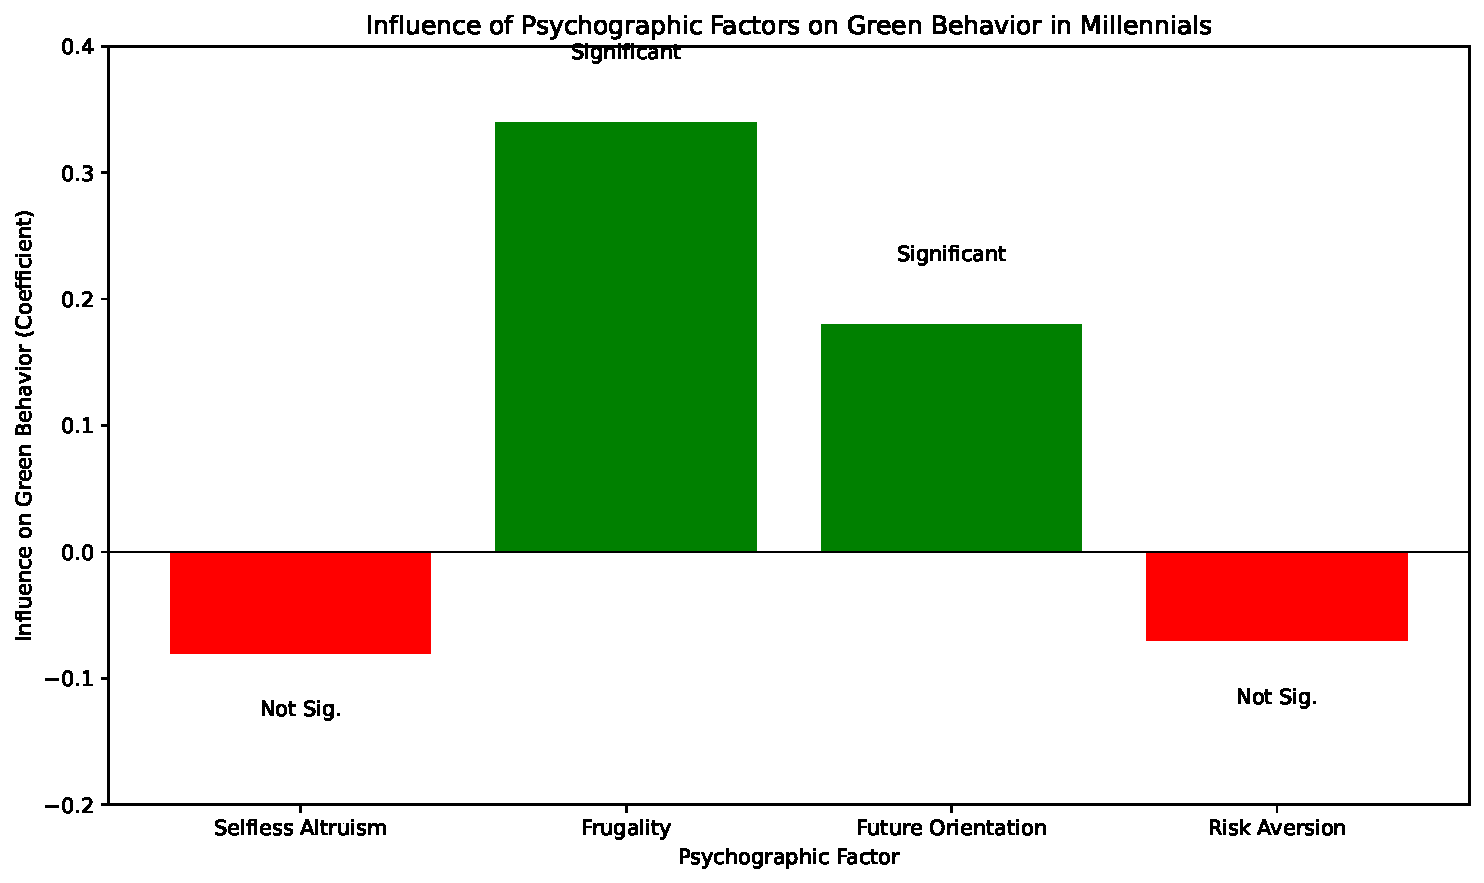
\includegraphics[keepaspectratio]{_thesis_files/figure-pdf/fig-mil-psych-sust-output-1.pdf}}

}

\caption[Psychological Factors Influencing Millennials to Engage with
Sustainability]{\label{fig-mil-psych-sust}Psychological factors
influencing millennials to engage with sustainability}

\end{figure}%

\subsection{Attitude-Behavior Gap}\label{attitude-behavior-gap}

While people express eco-conscious ideas, it's non-trivial to practice
sustainability in daily life. Translating eco-conscious attitudes into
concrete sustainable actions remains challenging. Empirical evidence
illustrates this gap between intention and behavior. (Park \& Lin, 2020)
positive attitude towards sustainable products does not result in
purchase decisions, shows research of fashion in South Korea. In one
Australian study, green consumers still waste food similarly to the
baseline (McCarthy \& Liu, 2017).

However, changing habits is important if technology alone is not the
solution. (Deyan Georgiev, 2023b) reports only 30\% of people in the
Gen-Z age group believe technology can resolve all environmental
problems. Even with good intentions, (Munro et al., 2023) finds shoppers
who try to shop sustainably often fail to find sustainable product, in a
systemic literature review of 64 papers from South Korea, Australia, the
UK, the US, and elsewhere.

\begin{itemize}
\item
  McKinsey says people want eco-products but aren't willing to pay more.
\item
  Willingness to pay research.
\end{itemize}

\subsection{Sustainability in Taiwan: Garbage Trucks and Digital
Receipts}\label{sustainability-in-taiwan-garbage-trucks-and-digital-receipts}

Musical garbage truck are a success story of the environmental progress
in Taiwan (Helen Davidson \& Chi Hui Lin, 2022). Indeed, they are a
\emph{user interface innovation} and the main way how people in Taiwan
interact with sustainability issues.

The popular narrative about Taiwan recounts the story of the economic
and environmental transformation of the country. In the late 1980s
during the heights of an economic boom Taiwan became famous as the
Taiwanese Miracle (臺灣奇蹟) (Gold, 1986; P.-L. Tsai, 1999). By the
early 1990s another less flattering nickname appeared: \emph{``garbage
island''}, for the piles of trash covering the streets and overflowing
landfills (Ngo, 2020; Rapid Transitions Alliance, 2019). In the two
decades that followed, from 1998 to 2018, Taiwan made progress in
municipal waste management, rising to the status of a world-leader in
recycling (2nd \emph{effective recycling rate} after Germany); in
addition to an effective recycling system, the average waste amount
generated per person by 700g (from 1140g to 400g) per day; nonetheless,
industrial recycling rates were less stellar, standing at 80\% in 2020
and there were unrealized opportunities in using industry 4.0
technologies, such as internet of things (IoT) sensors for better waste
tracking (Bui et al., 2023; C.-Y. Wu et al., 2021).

Progress in sustainability is possible but achieving results takes time
and innovation. (Rapid Transitions Alliance, 2019) credits the Taiwanese
Homemakers United Foundation (財團法人主婦聯盟環境保護基金會) for
initiating the transformation in 1987, suggesting a small group of
people can have an outsized impact on the whole country. Their activity
didn't stop there and (財團法人主婦聯盟環境保護基金會, 2020) recounts a
timeline of their achievements on their website until the present day.

({``{獨家觀察-電子發票年減碳量 相當2,700座大安森林公園},''} 2025)
reports 54.03\% of invoices in Taiwan are digital. Since 2021 digital
receipts are mandatory for all businesses. Taiwan's longstanding receipt
lottery also has specific prizes available only for digital receipts
(\emph{行動支付結合雲端發票 節能減碳最環保{\textbar}經理人}, 2018).
Several other countries, such as Singapore, South Korea, Japan, Sweden,
Italy, Portugal, Brazil, Mexico, have comparable systems in use.

\subsection{Trends in Taiwanese Industry and Online
Shopping}\label{trends-in-taiwanese-industry-and-online-shopping}

In the intensifying competition of online shopping in Taiwan,
(聯合新聞網, 2024) predicts Momo and Coupang will compete for Taiwanese
market leadership, with Coupang increasingly stepping on Shopee's and
MOMO's toes, as per ({``順風婦產科 순풍 산부인과 (@Followwindlover) on
{Threads},''} 2024).

Across online and offline, KANTAR reports Taiwan's consumer spending on
fast-moving consumer-goods (FMCG) grew over 5\% in 2024, speeding up
towards the end of the year: +2.5\% in Q1, +4.1\% in Q2, +5.7 \% in Q3
and +9.1\% in Q4, with e-commerce crossing the 20 \% share mark
(traditionally FMCG are purchased physical stores, as convenience stores
are so readily available all over Taiwan) (foodNEXT, 2024; Kantar
Worldpanel, 2024; 動腦Brain.com.tw, 2024; 食力 foodNEXT, 2025).

Taiwan has been on a path of change, striving to become more
sustainable. Between 1970 and 2019, emitting CO\textsubscript{2}eq was
largely a prerequisite for economic growth in Taiwan (T. Chang et al.,
2023). Since the 1990s, Taiwan is a net CO\textsubscript{2}eq exporter
through emissions embedded in the industrial production oriented economy
(R. Huang et al., 2020). Starting in 2023, Taiwan's Financial
Supervisory Commission's (FSC) added ``requirements for Taiwan's
corporates to disclose their carbon emissions,'' (Reformosatw, 2024).
Most recently, the Taiwanese environmental ministry has been cracking
down on illegal waste, with over 70 cases being prosecuted (環境部,
2025).

TIME Magazine and Statista collaborative \emph{``World's Most
Sustainable Companies Of 2024''} includes 17 Taiwanese companies (Alana
Semuels, 2024).

\def\pandoctableshortcapt{World's Most Sustainable Companies}

\begin{longtable}[]{@{}
  >{\raggedleft\arraybackslash}p{(\linewidth - 4\tabcolsep) * \real{0.3288}}
  >{\raggedright\arraybackslash}p{(\linewidth - 4\tabcolsep) * \real{0.3562}}
  >{\raggedleft\arraybackslash}p{(\linewidth - 4\tabcolsep) * \real{0.3151}}@{}}
\caption[World's Most Sustainable Companies]{World's Most Sustainable
Companies; data from (Alana Semuels, 2024).}\tabularnewline
\toprule\noalign{}
\begin{minipage}[b]{\linewidth}\raggedleft
\textbf{Sustainability Rank}
\end{minipage} & \begin{minipage}[b]{\linewidth}\raggedright
\textbf{Company}
\end{minipage} & \begin{minipage}[b]{\linewidth}\raggedleft
\textbf{Score (Out of 100)}
\end{minipage} \\
\midrule\noalign{}
\endfirsthead
\toprule\noalign{}
\begin{minipage}[b]{\linewidth}\raggedleft
\textbf{Sustainability Rank}
\end{minipage} & \begin{minipage}[b]{\linewidth}\raggedright
\textbf{Company}
\end{minipage} & \begin{minipage}[b]{\linewidth}\raggedleft
\textbf{Score (Out of 100)}
\end{minipage} \\
\midrule\noalign{}
\endhead
\bottomrule\noalign{}
\endlastfoot
24 & Delta Electronics & 77.18 \\
63 & Taishin Holdings & 73.50 \\
68 & Fubon Financial & 73.01 \\
80 & Chunghwa Telecom & 71.69 \\
91 & Yuanta Financial Holdings & 70.94 \\
92 & Cathay Financial Holdings & 70.79 \\
108 & Taiwan Mobile & 69.72 \\
200 & First Financial Holding & 64.17 \\
300 & Far EasTone & 60.04 \\
301 & SinoPac Holdings & 60.04 \\
344 & Wistron & 58.44 \\
356 & Acer & 58.02 \\
395 & Nanya Technology & 56.35 \\
409 & InnoLux & 55.82 \\
416 & Wiwynn & 55.67 \\
421 & Taiwan Cement & 55.49 \\
497 & Advantech & 53.14 \\
\end{longtable}

\let\pandoctableshortcapt\relax

Meanwhile, Corporate Knights which has been ranking global sustainable
companies since 2005, including analysis of 7000 public companies with a
revenue over US\$1 billion, only includes TSMC in the top 100 (placed
20th in 2021 and 44th in 2022, dropping out in 2023) and Taiwan High
Speed Rail Corp (THSR) and Giant Manufacturing Co Ltd since 2023
(Corporate Knights, 2024; Staff, 2021). Meanwhile, earth.org's list of
the world's 50 most sustainable companies in 2022, only includes 1
Taiwanese company - TSMC (Earth.Org, 2022).

\begin{figure}

\centering{

\pandocbounded{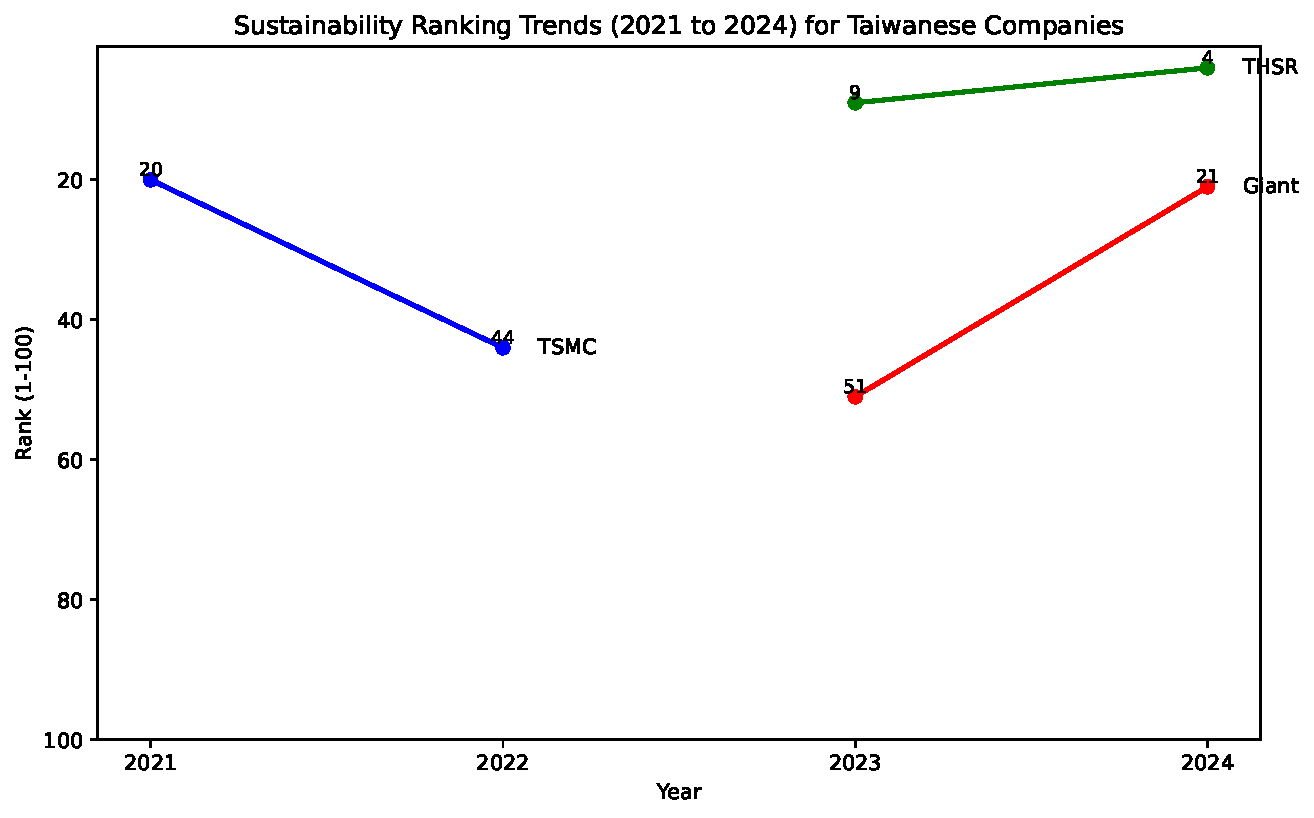
\includegraphics[keepaspectratio]{_thesis_files/figure-pdf/fig-tw-comp-rank-output-1.pdf}}

}

\caption[Taiwanese Company Ranking]{\label{fig-tw-comp-rank}Taiwanese
Company Ranking}

\end{figure}%

Meanwhile, (Marc Lien, 2022) finds 4 millions British SMEs have no plan
for net-zero transition and (Ware, 2024) adds, British workers lack
skills for green transition, according to a 2024 National Environmental
Services Survey.

\begin{figure}

\centering{

\pandocbounded{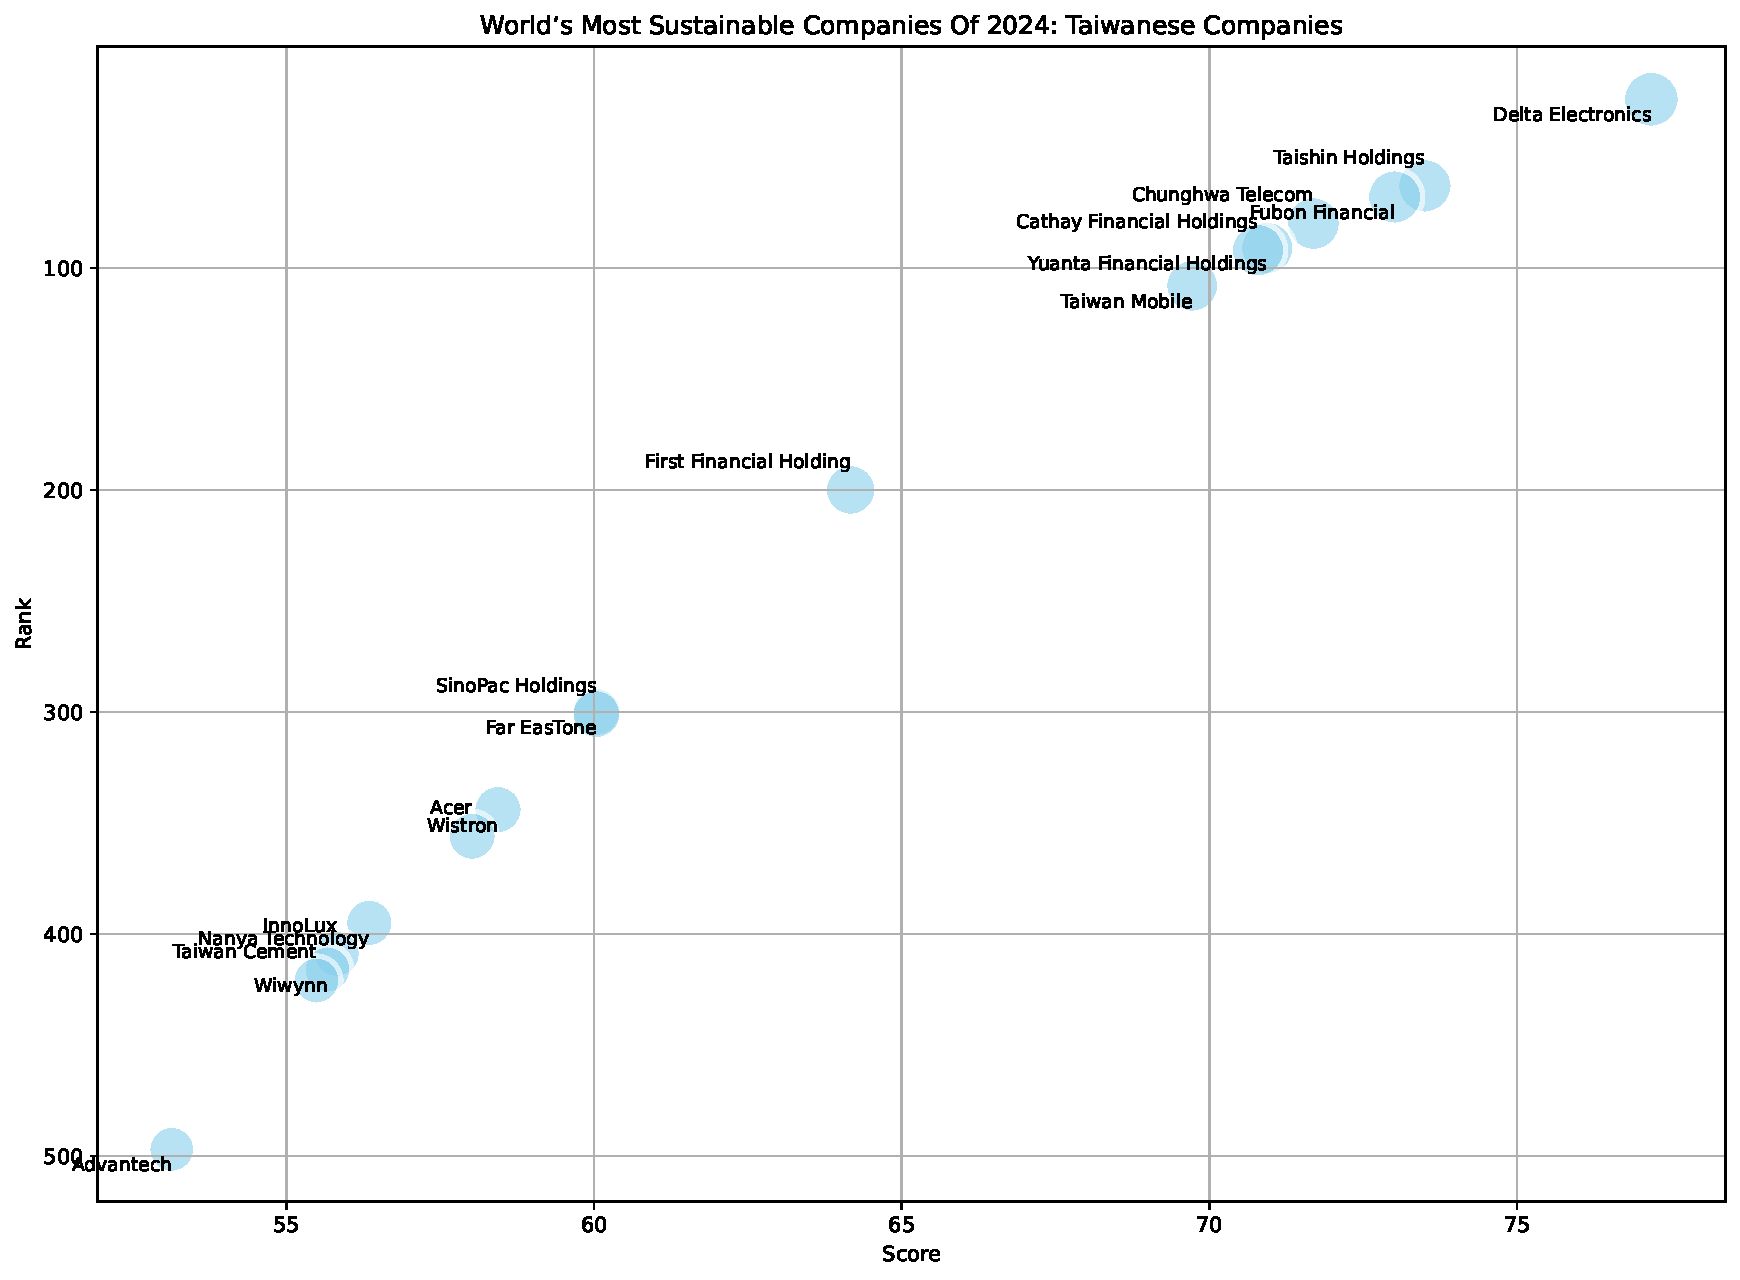
\includegraphics[keepaspectratio]{_thesis_files/figure-pdf/fig-br-comp-rank-output-1.pdf}}

}

\caption[British Company Ranking]{\label{fig-br-comp-rank}British
Company Ranking}

\end{figure}%

\subsection{Financial Literacy Worldwide and Among Taiwanese
Youth}\label{financial-literacy-worldwide-and-among-taiwanese-youth}

A recent nationwide study (n = 1997) titled Youth Financial Health
Basics (青少年財務健康基礎大調查) jointly conducted by the Taipei Fubon
Bank and the Parent-Child Innovation Center (親子天下教育創新中心)
between February 11 and March 9, 2025 found that over 65\% of secondary
schools incorporated financial-literacy courses into their curricula
however 64\% of Taiwanese youths (aged 15--18) exhibit low confidence
and understanding of financial products and face significant fraud risk,
with nearly 1/5 of the respondents encountering a scam in the past year,
while 18\% suffered actual financial losses (江昭倫, 2025; 陳美君,
n.d.).

\def\pandoctableshortcapt{Taiwanese Financial Product Familiarity}

\begin{longtable}[]{@{}lr@{}}
\caption[Taiwanese Financial Product Familiarity]{Familiarity with
financial products and preferred payment methods, as reported in
(陳美君, n.d.).}\tabularnewline
\toprule\noalign{}
\ul{\textbf{Banking}} & \ul{\% of Respondents} \\
\midrule\noalign{}
\endfirsthead
\toprule\noalign{}
\ul{\textbf{Banking}} & \ul{\% of Respondents} \\
\midrule\noalign{}
\endhead
\bottomrule\noalign{}
\endlastfoot
Have at least one financial account & 80\% \\
\ul{\textbf{Familiarity}} & \ul{\textbf{\% Unfamiliar}} \\
Savings accounts & 70\% \\
Mutual funds & 63\% \\
Stocks & 46\% \\
Deposit accounts & 30\% \\
\ul{\textbf{Payments}} & \ul{\textbf{\% Preference}} \\
Cash & 47\% \\
Family member pays & 47\% \\
EasyCard & 4\% \\
Mobile payments & 1\% \\
\end{longtable}

\let\pandoctableshortcapt\relax

Importantly for designing a financial app, while 80\% of the survey
respondents had received financial education at school, 90\% of the
students deemed the primary learning channel about financial knowledge
to be on social media; and only 15\% remember to have learned about
credit-card usage (江昭倫, 2025).

In a much older study, I-Cheng Yeh (2009) analyzed usage data from
30,000 credit-card clients at an undisclosed major Taiwanese bank to
predict next-month defaults, using 6 data-mining techniques including
ANNs (AI Neural Networks) (Yeh \& Lien, 2009). Because of the age of the
study there's no Gen-Z data. People aged 18-26 at the time would be
Millenials or Gen-X by now. the data was donated by (Yeh, 2016) and
roughly 1 in 5 credit card clients (22.1\%) of the dataset defaulted on
their payment in the next month. Among the 9,618 clients aged 18--29 at
the time of the study, 2,197 defaulted on their next‐month payment,
yielding a default rate of 22.8\%, slightly higher than the overall
average. Meanwhile, among the 5,127 clients aged 18--26, 1,285
defaulted, yielding a rate of 25.1\%, considerable higher than their
older counterparts. Finally, among the 1,558 clients aged 18--23, 430
defaulted, a rate of 27.6\%, pointing to a trend of younger people
having higher default rates.

A over-the-phone study (n = 3000) conducted in 2022, found Taiwanese
savings habits to have polarized, with over 60\% either having no
savings whatsoever or saving more than 1/2 of their annual income; 27\%
of respondents reported total savings below NT\$40,000; young adults'
(aged 20--29) were the only group whose financial risk worsened, with
43\% of the respondents having extremely low financial literacy,
described as 金融文盲 (near ``financial illiterate'') (中央社, 2022).

\def\pandoctableshortcapt{Financial Literacy Data from Phone Interviews}

\begin{longtable}[]{@{}
  >{\raggedright\arraybackslash}p{(\linewidth - 8\tabcolsep) * \real{0.5811}}
  >{\raggedleft\arraybackslash}p{(\linewidth - 8\tabcolsep) * \real{0.1351}}
  >{\raggedleft\arraybackslash}p{(\linewidth - 8\tabcolsep) * \real{0.0946}}
  >{\raggedleft\arraybackslash}p{(\linewidth - 8\tabcolsep) * \real{0.1081}}
  >{\raggedleft\arraybackslash}p{(\linewidth - 8\tabcolsep) * \real{0.0811}}@{}}
\caption[Financial Literacy Data from Phone Interviews]{Financial
literacy data from phone interviews, as reported in (中央社,
2022).}\tabularnewline
\toprule\noalign{}
\begin{minipage}[b]{\linewidth}\raggedright
Financial Literacy Among Taiwanese (2020)
\end{minipage} & \begin{minipage}[b]{\linewidth}\raggedleft
Very Low
\end{minipage} & \begin{minipage}[b]{\linewidth}\raggedleft
Low
\end{minipage} & \begin{minipage}[b]{\linewidth}\raggedleft
Medium
\end{minipage} & \begin{minipage}[b]{\linewidth}\raggedleft
High
\end{minipage} \\
\midrule\noalign{}
\endfirsthead
\toprule\noalign{}
\begin{minipage}[b]{\linewidth}\raggedright
Financial Literacy Among Taiwanese (2020)
\end{minipage} & \begin{minipage}[b]{\linewidth}\raggedleft
Very Low
\end{minipage} & \begin{minipage}[b]{\linewidth}\raggedleft
Low
\end{minipage} & \begin{minipage}[b]{\linewidth}\raggedleft
Medium
\end{minipage} & \begin{minipage}[b]{\linewidth}\raggedleft
High
\end{minipage} \\
\midrule\noalign{}
\endhead
\bottomrule\noalign{}
\endlastfoot
Overall financial literacy & 43.2\% & 34.9\% & 19.4\% & 2.5\% \\
Understanding products \& services & 34.0\% & 38.6\% & 23.1\% & 4.3\% \\
Confidence using products \& services & 30.0\% & 26.8\% & 37.6\% &
5.6\% \\
Seeking financial advice & 71.0\% & 3.2\% & 17.8\% & 8.0\% \\
Personal money management & 21.8\% & 42.9\% & 28.4\% & 6.9\% \\
\end{longtable}

\let\pandoctableshortcapt\relax

The Taiwanese Financial Literacy \& Education Association 財金智慧FINLEA
is a non-profit with a stated goal of enhancing financial literacy among
Taiwanese. Their longtitudinal study, with the latest survey conducted
in 2022 (n = 2014; 1055 high-school; 959 university) rated financial
literacy among all youths 56.3 out of 100 (53.8 in 2016 and 56.7 in
2007), always below the benchmark score of 60, with high school and
vocational students averaging 49.26 and university students somewhat
higher averaged 64.03 score (網軟股份有限公司, n.d.).

\def\pandoctableshortcapt{Taiwanese FINLEA Longitudinal Study}

\begin{longtable}[]{@{}
  >{\raggedright\arraybackslash}p{(\linewidth - 2\tabcolsep) * \real{0.6761}}
  >{\raggedleft\arraybackslash}p{(\linewidth - 2\tabcolsep) * \real{0.3239}}@{}}
\caption[Taiwanese FINLEA Longitudinal Study]{Latest report from the
財金智慧FINLEA longitudinal study (網軟股份有限公司,
n.d.).}\tabularnewline
\toprule\noalign{}
\begin{minipage}[b]{\linewidth}\raggedright
Knowledge Gap (2022)
\end{minipage} & \begin{minipage}[b]{\linewidth}\raggedleft
\% Unaware
\end{minipage} \\
\midrule\noalign{}
\endfirsthead
\toprule\noalign{}
\begin{minipage}[b]{\linewidth}\raggedright
Knowledge Gap (2022)
\end{minipage} & \begin{minipage}[b]{\linewidth}\raggedleft
\% Unaware
\end{minipage} \\
\midrule\noalign{}
\endhead
\bottomrule\noalign{}
\endlastfoot
Unsure that employers must contribute to the labor pension (and
individuals can voluntarily contribute) & 68\% \\
Unsure which deductions (income tax, labor insurance, health insurance)
reduce take-home pay & 66\% \\
Unsure how education level affects starting salary & 61\% \\
Unaware of methods to lower loan interest rates & 59\% \\
Cannot identify which auto insurance covers vehicle damage & 55\% \\
Unable to judge which life-insurance need is greatest & 51\% \\
Uncertain how to choose investment tools for maximum lifetime returns &
63\% \\
Unaware that business tax makes purchases more expensive & 61\% \\
\end{longtable}

\let\pandoctableshortcapt\relax

財金智慧FINLEA does publish online videos targeted at young people,
however as of early 2025, they only have around 1000 subscribers on
YouTube (財金智慧FINLEA, 2020). Meanwhile the Taiwanese cryptocurrency
influencer Mr Block has over 100000 YouTube subscribers (mrblock
區塊先生, 2025).

\begin{figure}[H]

{\centering 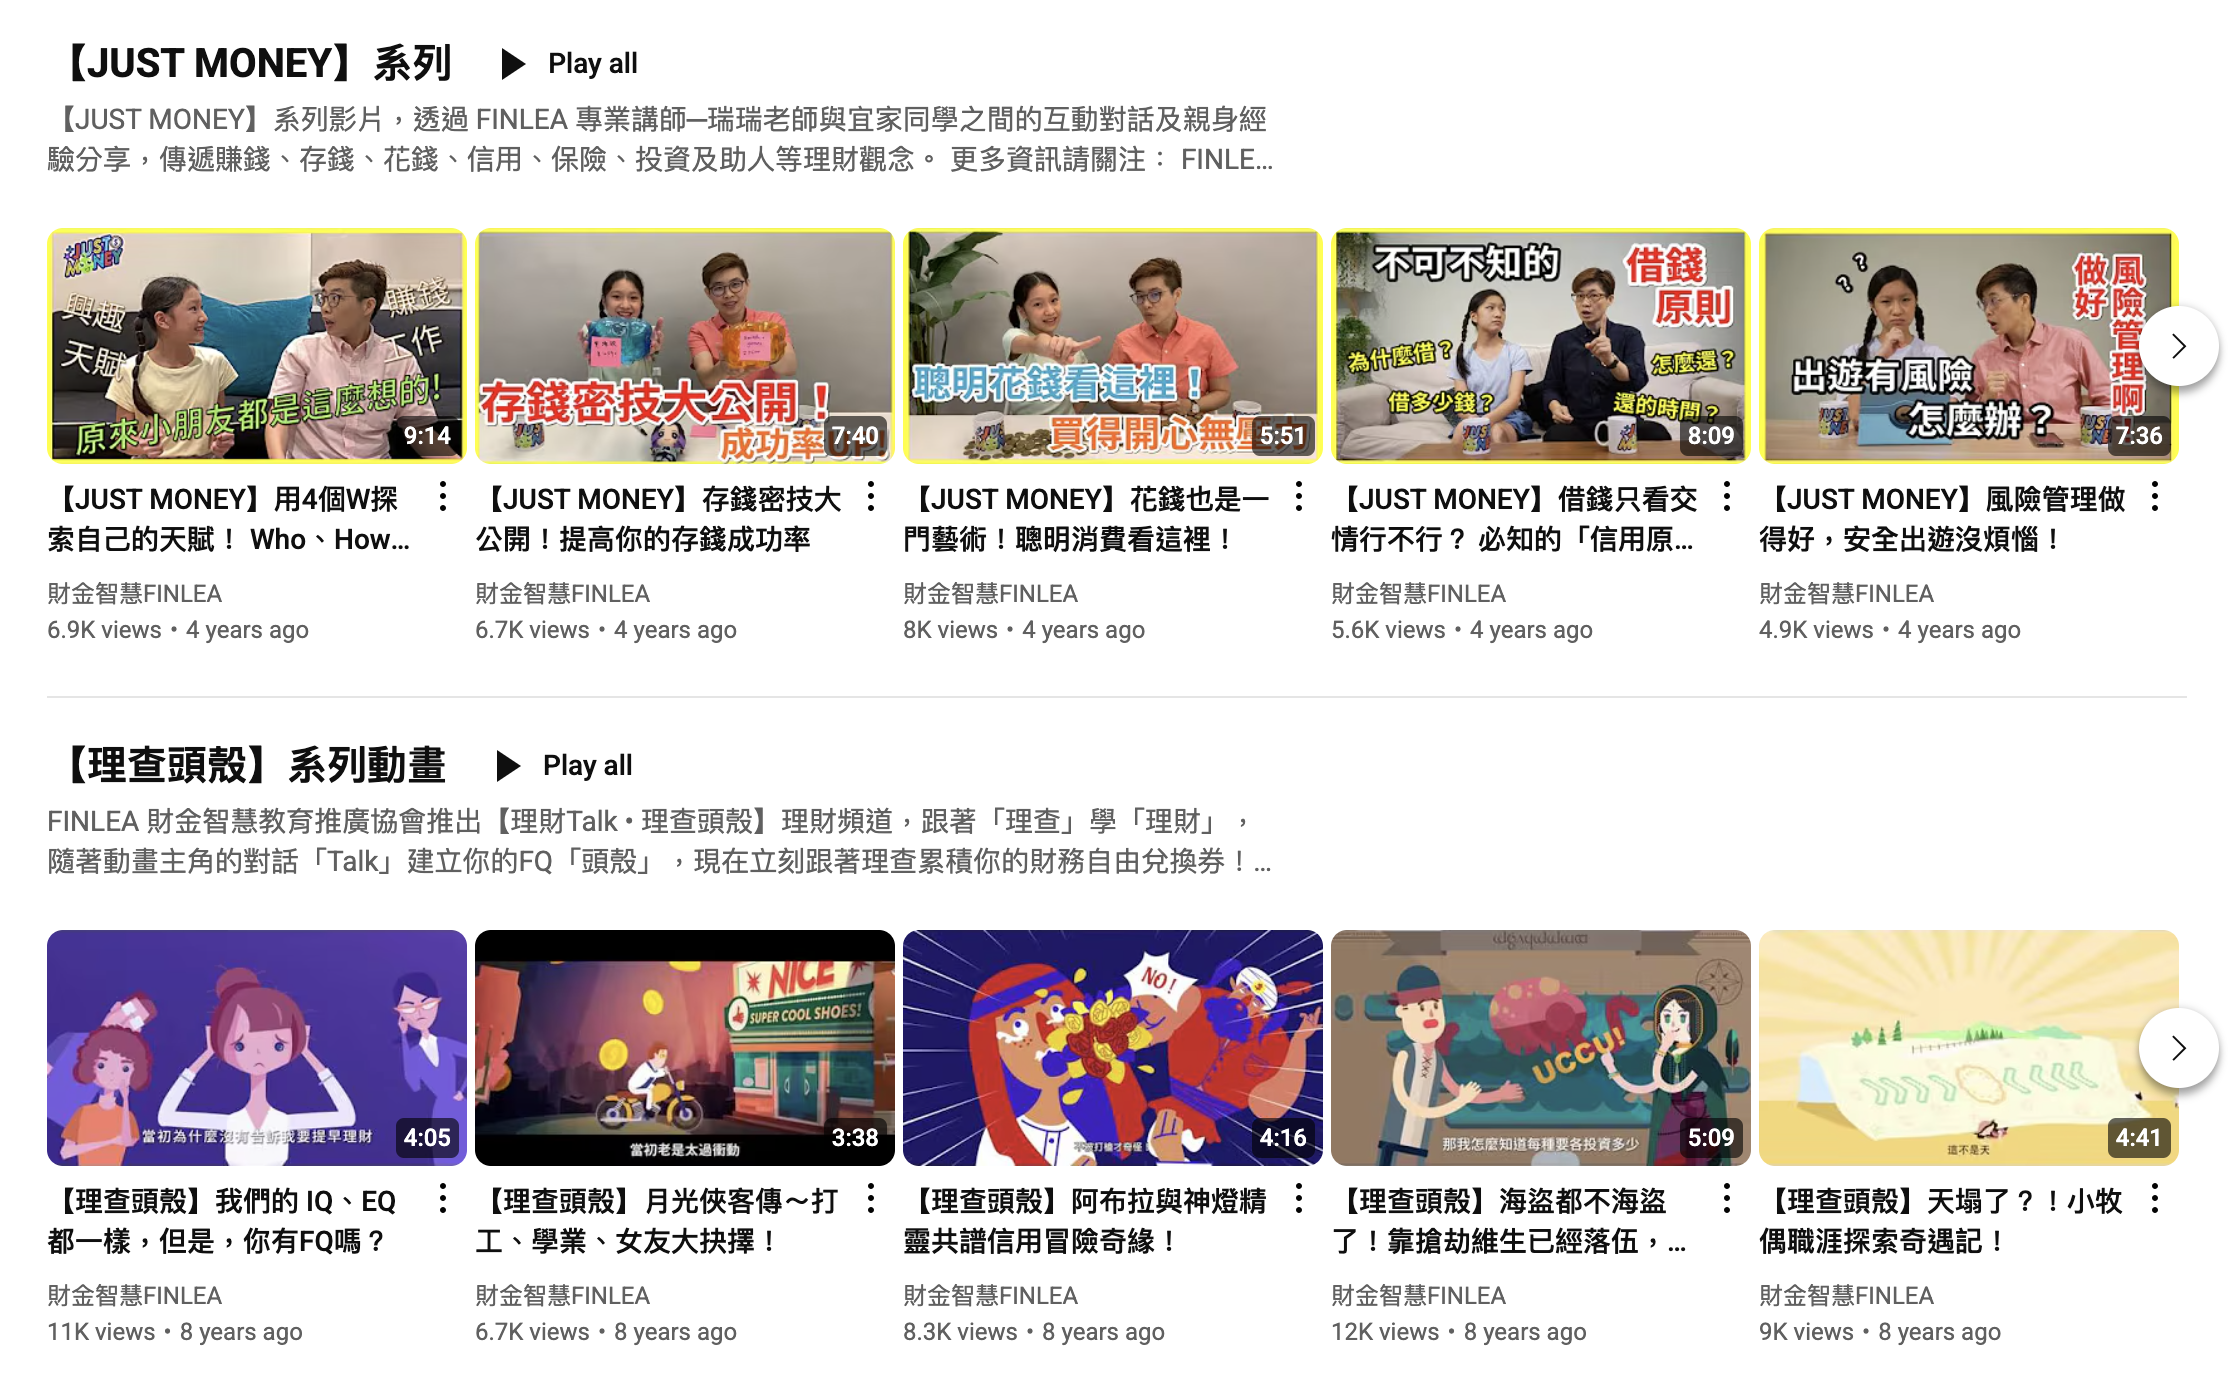
\includegraphics[width=1\linewidth,height=\textheight,keepaspectratio]{./images/college/taiwan-financial-literacy-youtube.png}

}

\caption{財金智慧FINLEA YouTube Channel}

\end{figure}%

Internationally, there's evidence young people have money. In the United
States, the combined annual consumer spending of Gen-Z and Millennials
was over \$2.5 Trillion in 2020 (YPulse, 2020). Over the decade from
2020 to 2030, in the U.S., UK, and Australia, Millennials are projected
to inherit \$30 Trillion USD from their parents (Calastone, 2020).
(Steverman, 2022) puts the inheritance figure between 2022-2045 at an
higher \$73 Trillion USD. There's also some evidence of investment
interest, however with a large geographic variance. According to a
(Calastone, 2020) study (n = 3000) surveying people in the millennial
age group between ages 23 and 35 in Europe (UK, France, Germany),
U.S.A., Hong Kong, and Australia, 48\% of respondents located in Hong
Kong owned financial securities (such as stocks) while the figure was
just 10\% in France.

\def\pandoctableshortcapt{Millennial Investors}

\begin{longtable}[]{@{}ll@{}}
\caption[Millennial Investors]{Data from millennial investors
(Calastone, 2020).}\tabularnewline
\toprule\noalign{}
Place of Comparison & Financial Security Ownership \\
\midrule\noalign{}
\endfirsthead
\toprule\noalign{}
Place of Comparison & Financial Security Ownership \\
\midrule\noalign{}
\endhead
\bottomrule\noalign{}
\endlastfoot
Hong Kong & 48\% \\
France & 10\% \\
& \\
\end{longtable}

\let\pandoctableshortcapt\relax

\subsection{Social Media, Trends, Memes, and Youth
Empowerment}\label{social-media-trends-memes-and-youth-empowerment}

The term ``meme,'' first coined by Richard Dawkins in 1976 in his book
``The Selfish Gene'' to describe units of cultural evolution, analogous
to that of biological evolution, which may evolve by natural selection,
and now encompasses internet artifacts and even stocks. Beyond mere
entertainment, memes have emerged as an academic discipline, where memes
are sampled, coded, and analysed from cultural and ethical viewpoints,
among others (Zidani \& Miltner, 2022). (Peters-Lazaro et al., 2020)
argues memes are no merely jokes but tools for communal critique and
collective visioning. suggesting that Taiwanese Gen-Z memes scaffold
deeper conversations about consumerism, climate action, and social
change. Memes from daily life, business to war, are relevant to
penetrating through the noise of the web.

In Taiwan, homegrown memes may start with global templates but quickly
take on a local flavor. (劉芸嘉, 2024)'s 2021 study of 150 Taiwanese
memes written in Mandarin shows most rely on friendly and indirect
humor: inside jokes and wordplay that bond peers together.
(朱映潔(Ying-Chieh Chu), 2021) surveyed 737 Taiwanese Facebook users and
discovered that a meme's funniness, shareability, and shock value
``hellish gags'' (地獄梗) drive people to post it for social approval.
(胡綺珍, 2024) collected 217 ``tired of life'' / ``I'm just trash'' meme
texts from Instagram and PTT, then interviewed 13 Gen-Z enthusiasts,
revealing how self-deprecating jokes help Gen Z cope with stress, feel
part of a group, and quietly push back against social pressure. Memes
have a long history, and even almost a decade ago in 2016, a casual news
comment---like the ``canoing man'' (泛舟哥) remark during a typhoon
exploded into LINE stickers and PTT threads, proving that Taiwanese can
transform everyday media moments into collective satire or
tongue-in-cheek commentary (黃意能 \& 黃曉琪, 2016).

Internationally, the sustainability-focused topics ``underconsumption''
and ``deinfluencing'' were trending on TikTok in 2024 however have since
subdued (Fares et al., 2024; TikTok, 2024b, 2024a). While this
particular trend may be over, memes still hold potential for
communicating about sustainability to young Taiwanese. Still, looking at
older international data, (Zannettou et al., 2018) built a large-scale
machine-learning pipeline to trace the origin of memes in the US, with
160M images and 2.6B posts within about 1 year (July 2016-2017) from
Twitter, Reddit, 4chan and Gab, finding that often memes originate from
fringe communities and then spread across mainstream media, highlighting
how fringe communities can be surprising impactful.

In Taiwan, Internet usage among young people is nearly universal, with
over to 98\% of 18--29 (roughly Gen-Z) year‐olds reporting they have
gone online at least once recently, and close to 96\% of respondents
aged 18-29 used some form of social media (財團法人台灣網路資訊中心 \&
台灣資訊社會研究學會, 2023).

\def\pandoctableshortcapt{Taiwanese Internet Usage Statistics}

\begin{longtable}[]{@{}lll@{}}
\caption[Taiwanese Internet Usage Statistics]{Taiwanese Internet Usage
Statistics; data from (財團法人台灣網路資訊中心 \& 台灣資訊社會研究學會,
2023).}\tabularnewline
\toprule\noalign{}
Metric & 18--29 & 30--39 \\
\midrule\noalign{}
\endfirsthead
\toprule\noalign{}
Metric & 18--29 & 30--39 \\
\midrule\noalign{}
\endhead
\bottomrule\noalign{}
\endlastfoot
Daily Internet usage & 98.79 \% & 98.40 \% \\
Overall social-media usage & 95.98 \% & 94.84 \% \\
TikTok usage & 33.03 \% & 24.28 \% \\
\end{longtable}

\let\pandoctableshortcapt\relax

(林高賢, 2024) analyzed (n = 1175) Taiwanese high school students,
mostly aged Gen-Z, finding that Instagram (IG) dominates, used by close
to 85\% percent of the respondents; they use IG for about 2 hours per
day, 5-6 days per week; moreover, respondents often feel anxious (1-2
days per week), and anxiety correlates with several motivations of using
IG, such as recording life moments, documenting travel, food, and
fitness with photos, was tied to higher anxiety, possibly related to the
photo-centric self-presentation on Instagram, why can be theorized to
heighten sensitivity to feedback and criticism. In contrast, (陳思凝,
2023) conducted a survey of 458 Taiwanese Gen Z Instagram users, finding
that higher Instagram use intensity is directly associated with greater
online subjective well-being; however, intense use also leads to
information overload and social comparison, which induce social media
fatigue and in turn erode well-being; moreover, users' perceived
intimacy with the platform amplifies the link between use intensity and
social comparison frequency. An online survey by (廖柏雅, 2024) (where
the Gen-Z cohort n = 125) found respondents to be highly motivated by
social and entertainment use; the user's fear of missing out (FoMO) was
found to be related to the motive; e.g.~people with social and
entertainment drives experience greater FoMO than those motivated
primarily by information seeking. (Lasnik, 2018) surveys college
students at the National Dong Hwa University in Hualian (n = 300, a mix
of Taiwanese and international students), using the Liebowitz Social
Anxiety Scale (LSAS) and Taijin Kyofusho Scale (TKS) as research
instruments, finding Taiwanese students ranked higher on the Taijin
Kyofusho, suggesting the fear of offending or disturbing others is
stronger among local students.

A large-scale (n = 2075) representative face-to-face survey among people
aged 18 to 93 years in Taiwan (no age-based categorization was published
for Gen-Z specifically), found that in general sharing one's thoughts
online (known academically as ``self-disclosure'') boosts perceived
social support and significantly boosts bonding and bridging social
capital, which increases life satisfaction and lowers loneliness (樊一寧
et al., 2024). Conversely, in Japan, while not directly comparable,
Gen-Z reports wanting privacy and 75\% feel others overshare on social
media and 49 percent were concerned about their personal data (McKinsey
\& Company, 2022).

\subsection{AI Use Among Taiwanese
Students}\label{ai-use-among-taiwanese-students}

A survey of college students in March 8--10, 2023 at the Chung Yuan
Christian University (n = 983) in Taoyuan (Northern Taiwan), yielded the
following results: 66\% of the students had used ChatGPT, with the the
top use cases being summarization (31\%), translation of articles
(28\%), and writing reports (24\%) (CYCU, 2023; 許維寧, 2023). However,
in terms of AI adoption, this data can be considered out-dated. ChatGPT
was first released to the public on November 30, 2022, so the students
had had only about 3 months to try it out (OpenAI, 2022). At the time,
the GPT-3.5 model was available; the revolutionary GPT‑4 was released to
the public on March 14, 2023, (OpenAI, 2023).

In a more recent large-scale survey focusing on AI literacy administered
to the general public (n = 2174) found that only 26\% of the respondents
had used ChatGPT in the past 3 months (in comparison with the 25\% from
a similar survey administered in the previous year); younger people had
higher usage patterns, 53\% for 18-29 and 37\% 30-39; meanwhile, 69\% of
respondents believed they could tell the difference between AI-generated
and non-AI content and 73\% supported some type of government
regulations for AI (HakkaNews, 2024).

A Chinese study from two authors at the Minzu University and Beijing
Normal University reports they recruited anonymous Taiwanese college
students (n = 916) on the Chinese Credamo platform from the Taiwanese
IP-space (ChatGPT is blocked in Mainland China, Macau, and Hong Kong) to
compare ChatGPT vs.~Google for academic use among Taiwanese students:
their findings show a clear preference for ChatGPT overall, which
students deemed more flexible (meanwhile some older students still
preferred Google) and Random Forest and LightGBM-based modeling
predicted tool choice by three main factors: 1) GenAI fluency,
2)awareness of GenAI hallucinations, and 3) user age; their
recommendations include 1) support critical-thinking among users, and 2)
design hybrid chat+search user interfaces with higher reliability
(Kelly, 2024; Qiao \& Lee, 2024; M. Zhang \& Yang, 2024). In the US, an
older study of young adults (Millenials at the time) highlights how they
\emph{``use Google as a reference point for ease of use and
simplicity'',} (Kate Moran, 2016). The web now has several generations
of native users, and some older usage patterns which older digital
natives are used to, may take time to change.

In Sweden, a large-scale (n = 5894) survey across several Swedish
universities showed college students' attitudes towards AI assistants
(ChatGPT was by far the most prevalent app, 95 \% of respondents had
heard of ChatGPT and 35 \% used it regularly); 55.9\% held a positive
attitude toward AIs; integrity was a hotly debated question, 62\%
calling AI use in exams ``cheating,'' but 60\% rejecting an outright
ban, and 58\% saying it doesn't violate the purpose of education (Stöhr
et al., 2024).

\begin{figure}

\centering{

\pandocbounded{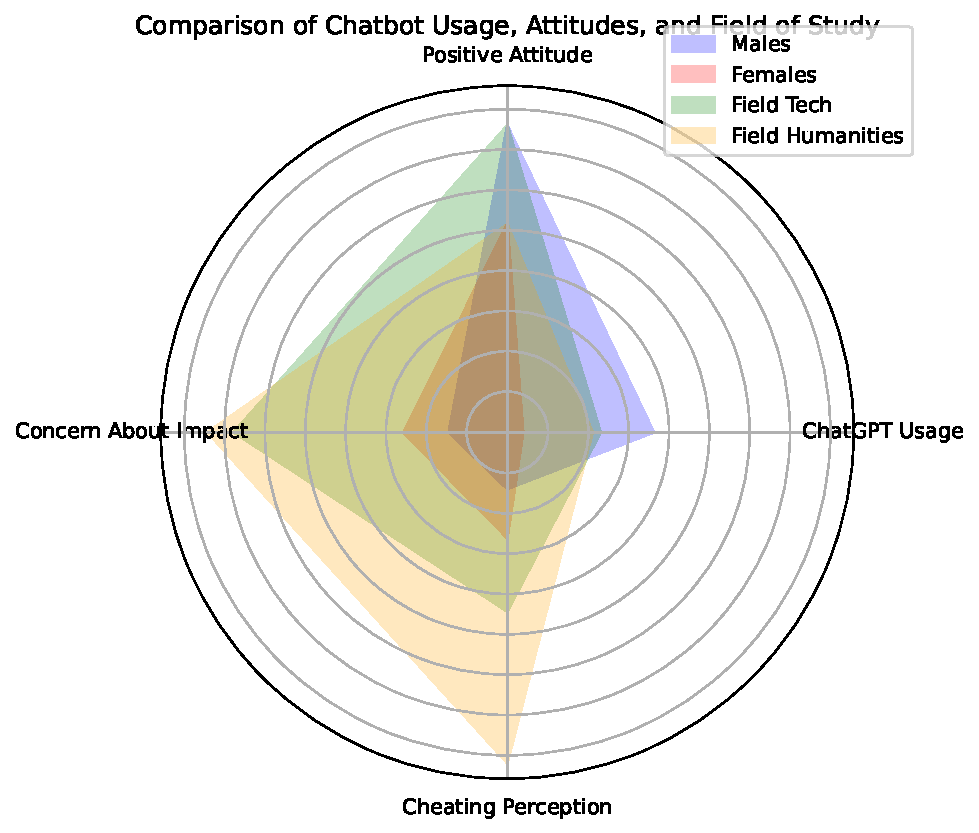
\includegraphics[keepaspectratio]{_thesis_files/figure-pdf/fig-college-chatbot-output-1.pdf}}

}

\caption[Swedish College Students' Attitudes Towards AI
Assistants]{\label{fig-college-chatbot}Swedish College Students'
Attitudes Towards AI Assistants}

\end{figure}%

\newpage

\section{Sustainability}\label{sustainability}

\begin{figure}[H]

{\centering \pandocbounded{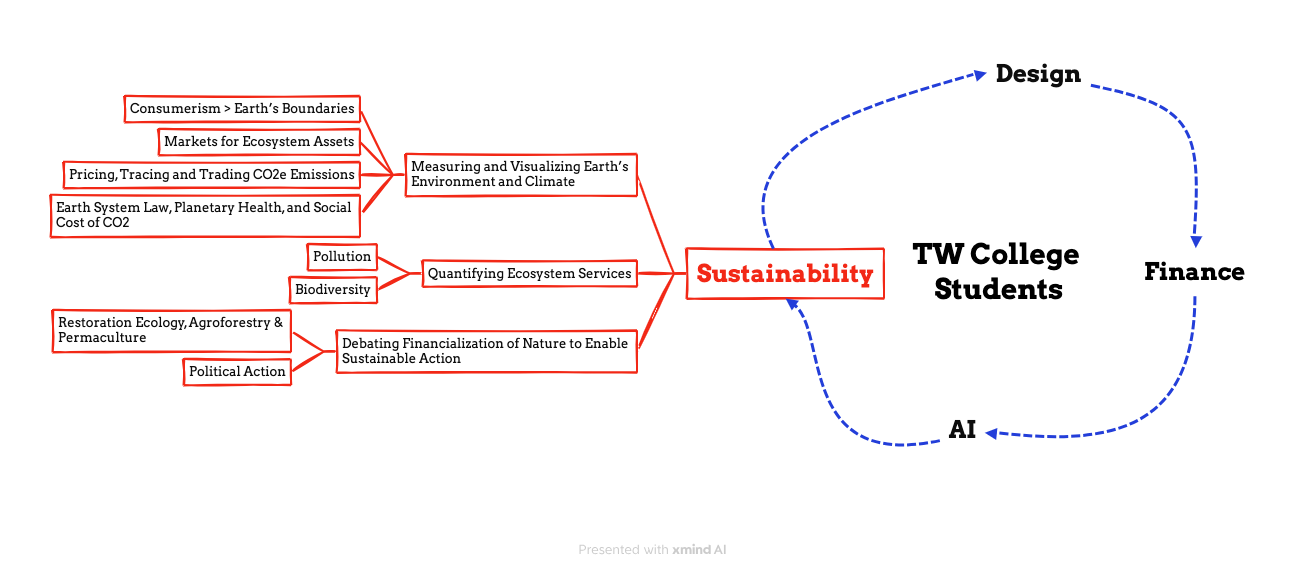
\includegraphics[keepaspectratio]{./images/sustainability/abstract-sustainability.png}}

}

\caption{Visual abstract for the sustainability chapter}

\end{figure}%

\subsection{The Roots of Sustainability in
Environmentalism}\label{the-roots-of-sustainability-in-environmentalism}

\emph{``Nachhaltigkeit''} - \emph{sustainability} in German - was likely
the first use of the concept of preserving natural resources, conceived
by a tax accountant Hannß Carl von Carlowitz in 1713 in his seminal book
on forestry - \emph{Sylvicultura oeconomica -}, referring to the goal of
achieving prudent forest management practices in his native Saxony in
Southeastern Germany, which at the time was under severe
\emph{deforestation} pressure from mining, ship-building and
agricultural production (Gottschlich \& Friedrich, 2014; Hannß Carl von
Carlowitz, 1713). This particular field of sustainability study is now
known as \emph{sustainable yield of natural capital}. The
\emph{principal} of the natural resource being managed, such as in
fishing and forestry, shouldn't be over-harvested in order to maintain
\textbf{\emph{ecosystem services}} - a contemporary term from the theory
of \emph{natural capital}, referring to benefits humans receive from the
stock of world's natural resources (Peter Kareiva et al., 2011).

Defining sustainability perhaps more poetically, the American wildlife
ecologist Aldo Leopold proposed the idea of \emph{land ethics} in 1972
as \emph{``{[}a{]} thing is right when it tends to preserve the
integrity, stability, and beauty of the biotic community. It is wrong
when it tends otherwise''} in his landmark work \emph{A Sand County
Almanac} (Leopold, 1972). In a similar vein, the 1987 United Nations'
Brundtland Report titled ``\emph{Our Common Future''} defined
\emph{sustainable development} as \emph{``Development that meets the
needs of the present without compromising the ability of future
generations to meet their own needs''} (World Commission on Environment
and Development, 1987). Given these varied ideas for over 300 years, I
believe some percentage of people have been concerned with our planet's
natural environment and its preservation already for centuries. Yet, it
is only in the last 100 and so years that human activities have begun to
affect Earth's systems on a previously unseen scale - termed
\emph{Anthropocene} -, necessitating a deeper understanding of
human-nature interactions, such as in the case of climate change, which
is rapidly changing the face of our living environments.

\subsection{Measuring and Visualizing Earth's Climate
Systems}\label{measuring-and-visualizing-earths-climate-systems}

Studies of Earth's climate go back for over 200 years, starting with
Alexander von Humboldt,the founder of climatology, who revolutionized
cartography by inventing the first \emph{isothermal maps} in 1816; these
maps showed areas with similar temperature, variations in altitude and
seasons in different colors (Honton, 2022) now available as 3D computer
models(\emph{Alexander von {Humboldt}'s Original Isotherms Circa 1838},
2023). Already in 1896, the Nobel Prize winner Svante Arrhenius first
calculated how an increase in CO\textsubscript{2} levels could have a
warming effect on our global climate (Anderson et al., 2016; Wulff,
2020). In 1938, Guy Stewart Callendar was the first scientist to
demonstrate the warming of Earth's land surface as well as linking the
production of fossil fuels to increased CO\textsubscript{2}e and
changing climate (Hawkins \& Jones, 2013). Early scientists pioneered
climate modeling by calculating the first climate interactions which
precede today's complex computer-based \emph{Earth System Models (ESMs)}
that integrate the various Earth systems and cycles run on
supercomputers (Anderson et al., 2016).

\begin{figure}[H]

{\centering 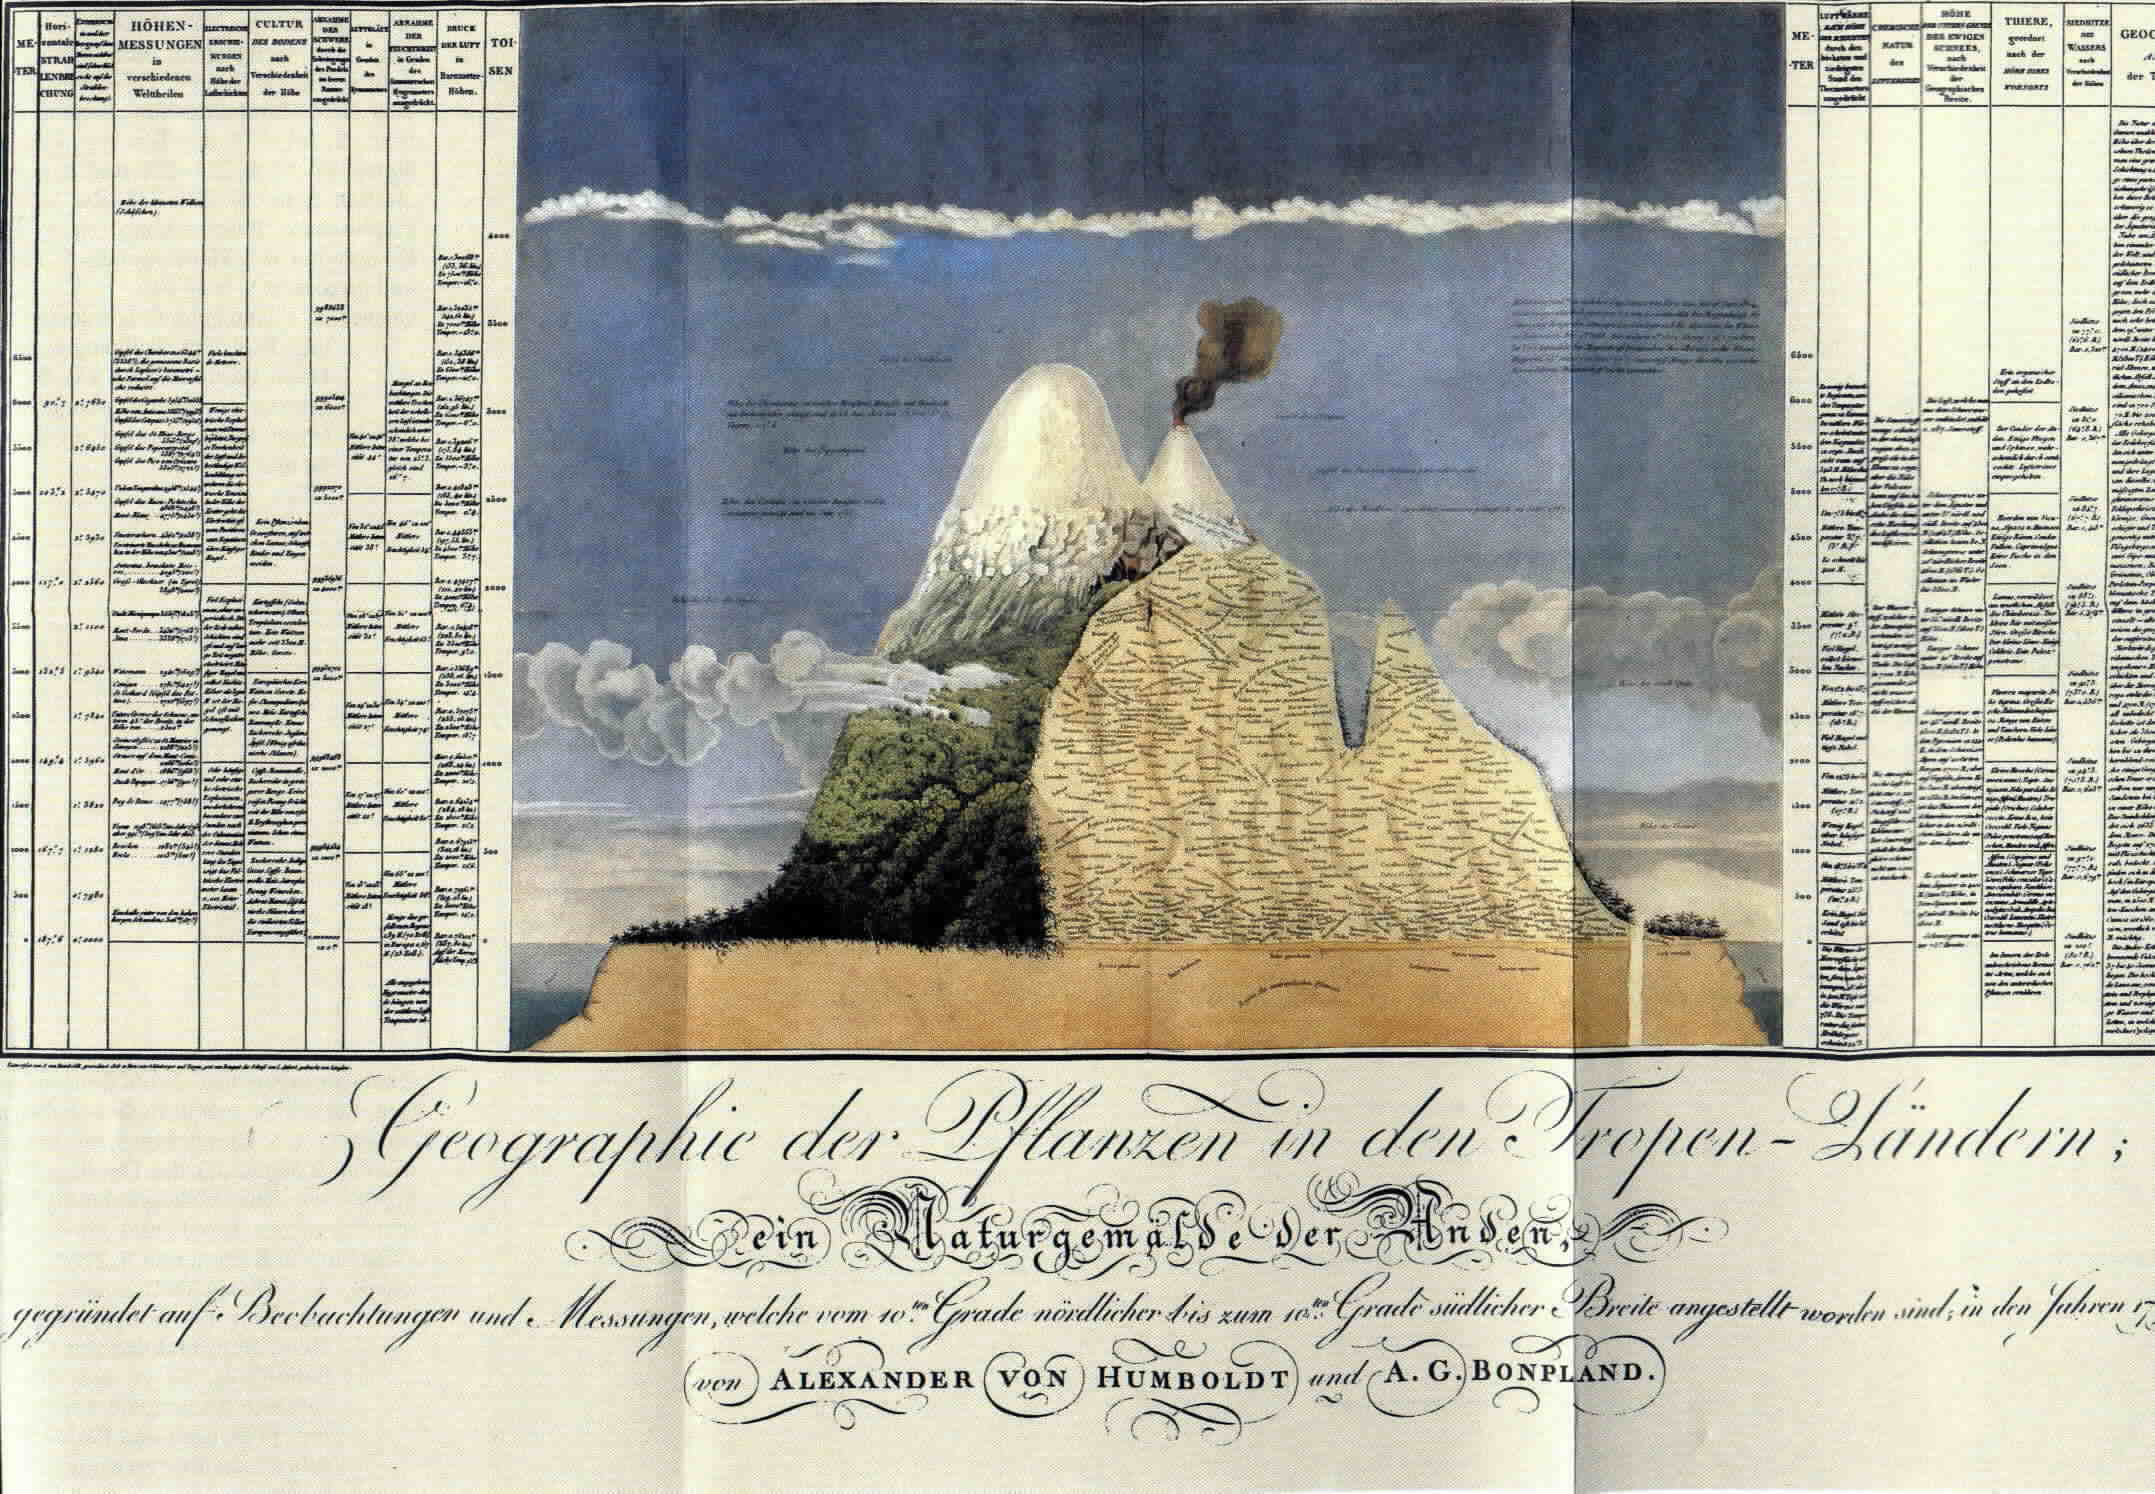
\includegraphics[width=1\linewidth,height=\textheight,keepaspectratio]{./images/sustainability/humboldt.jpg}

}

\caption{Humboldt's Naturgemälde, early data visualization of ecology,
rain, temperature, elevation, etc}

\end{figure}%

Environmental activists have been calling attention to global warming
for decades, yet the world has been slow to act (McKibben, 1989). While
the scientific case for human-induced climate change was building, it
took 120 years after Arrhenius' calculations, until the Paris Climate
Agreement in 2016, that countries came to an agreement on non-binding
targets on keeping CO\textsubscript{2} levels 1.5 °C below
pre-industrial levels (defined as 1850--1900)(United Nations, 2016).
Even though awareness of Earth's warming climate was growing ever
stronger, the CO\textsubscript{2} emissions kept rising too. The
hockey-stick growth of CO\textsubscript{2} concentration since the
industrial revolution is clear in the data from 1958 onward, following a
steady annual increase, called the \emph{Keeling Curve} (Keeling \&
Keeling, 2017). Written records of global temperature measurements are
available starting from the 1880s, when temperatures began to be
documented in ship logs (Brohan et al., 2012). Finally, although perhaps
less accurately, temperature estimations from tree-trunks allow some
comparisons with the climate as far back as 2000 years ago (Rubino et
al., 2019).

April 2025 was Earth's 2nd-warmest April on record, with global
temperatures reaching 1.32°C above the 20th-century average, driven by
persistent El Niño conditions and record-high ocean temperatures
(Masters, 2025). This warming aligns with growing concerns about Earth's
energy imbalance, which recent satellite data suggest has nearly doubled
since 2005; more heat is being trapped in the climate system than is
being radiated back to space (Mauritsen et al., 2025). Compounding the
issue, 3 key NASA climate satellites responsible for monitoring Earth's
energy budget are nearing the end of their operational life with no
replacement missions currently planned, raising alarms about the
continuity and reliability of future climate data (Harvey, 2025).
Likewise, funding for the Scripps Institute, responsible for the Keeling
Curve, is under threat, according to its caretaker, Ralph Keeling.

The Keeling Curve apparatus measures absorption of infrared light, which
allows one to detect the amount of CO\textsubscript{2}eq in the air. It
also has an advanced calibration system where it makes measurements in
air with a known quantity of gases (Worthington, 2025b).

\begin{figure}

\centering{

\pandocbounded{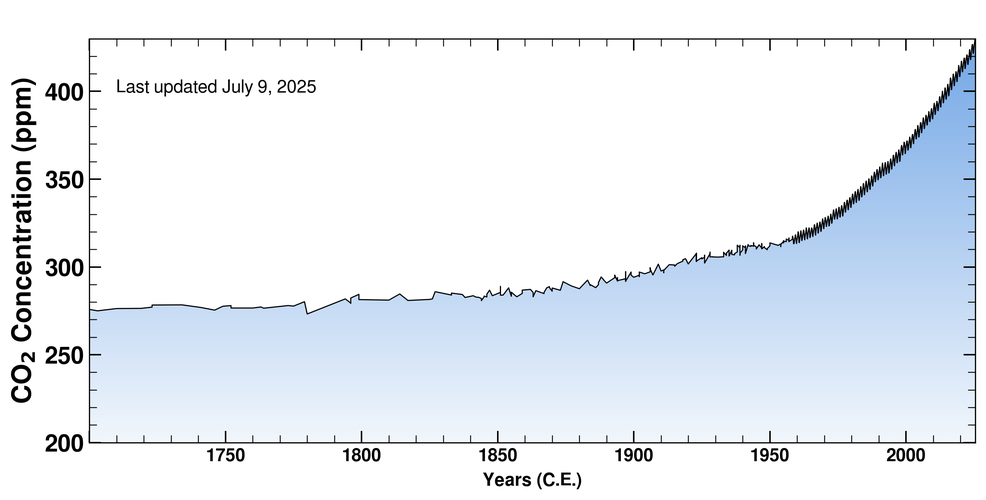
\includegraphics[keepaspectratio]{./images/sustainability/co2-concentration.png}}

}

\caption[Atmospheric CO\textsubscript{2} Concentration
(2025)]{\label{fig-co2-concentration}CO\textsubscript{2} concentration
in the atmosphere as of 2025. Image Credit: Scripps Institution of
Oceanography at UC San Diego.}

\end{figure}%

The latest data from 2023 shows our current world population of 8
Billion people emitted 37.2 gigatonnes (i.e.~billion metric tons) of
CO\textsubscript{2}e per year, the highest emissions recorded in history
(Statista, 2023a). Since 1751, cumulative CO\textsubscript{2}eq
emissions have exceeded 1.5 trillion tonnes globally or when expressed
in CO\textsubscript{2}eq for all green house gases, total historic
emissions would reach roughly 1.7 trillion tonnes CO\textsubscript{2}eq
since the start of the Industrial Revolution.(Global Carbon Budget,
2023; Marvel, 2023). In order to limit global warming to 1.5 °C as
agreed by the world nations in Paris, removal of 5-20 gigatons of
CO\textsubscript{2}e per year would be needed according to reduction
pathways calculated by the Intergovernmental Panel on Climate Change
(IPCC) (UNFCCC. Secretariat, 2022; Wade et al., 2023). Yet, most
countries are missing the mark (Climate Analytics \& NewClimate
Institute, 2023; United Nations Environment Programme, 2023). The
European Union's Copernicus Climate Change Service (C3S) reports 1.5 °C
global warming has already been breached in 2024 temperatures ({``First
Time World Exceeds 1.{5C} Warming Limit over 12-Month Period,''} 2024;
\emph{World's First Year-Long Breach of Key 1.{5C} Warming Limit},
2024). Given the current pace of climate change action, the G7 countries
(Canada, France, Germany, Italy, Japan, United Kingdom, United States)
are heading for 2.7 °C of warming by 2050 (CDP, 2022).

(United Nations Environment Programme (UNEP), 2021) reported as of 2021
updated national climate pledges (NDCs) and other mitigation measures
are projected to lead to a global temperature increase of approximately
2.7°C by 2100, significantly surpassing the Paris Agreement's
aspirational goal to keep global warming below 1.5°C this century;
effective implementation of net-zero emissions pledges could still keep
warming around 2.2°C (approaching the Paris Agreement's goal of below
2°C), if countries cut methane emissions from fossil fuel, waste, and
agricultural sectors, bridging the current emissions gap - and carbon
markets might significantly cut emissions, if they are governed by clear
rules ensuring genuine emission reductions, alongside transparent
systems for monitoring and tracking progress - however, numerous
national climate strategies postpone substantial action until after
2030. A year later, the 2022 Emissions Gap report showed a somewhat
worsening situation, with existing national pledges leading the world
for around 2.8 °C of warming by 2100 (United Nations Environment
Programme, 2022)

Earth's physical systems are very sensitive to small changes in
temperature, which was not understood until the 1970s(McKibben, 2006). A
comprehensive review of evidence from paleoclimate records until current
time, including ocean, atmosphere, and land surface of points towards
substantial climate change if high levels of greenhouse gas emissions
continue, termed by the authors as \emph{climate sensitivity} (Sherwood
et al., 2020). Global warming may lead to the slowing down and complete
stop of the Atlantic meridional overturning circulation (AMOC) which
helps maintain climate stability (Ditlevsen \& Ditlevsen, 2023). Apart
from CO\textsubscript{2}, reduction of other atmospheric pollutants,
such as non-CO\textsubscript{2} greenhouse gases (GHGs) and short-lived
climate pollutants (SLCPs) is required for climate stability (J. Lin et
al., 2022).

(Armstrong McKay et al., 2022a; TED, 2024) warns that climate is not a
linear system, rather there are several non-linear climate tipping
points, where change accelerates: at the current warming ice‐sheet
collapse, permafrost thaw, Amazon dieback and coral‐reef loss are likely
to tip between 1.5 °C and 2 °C, underscoring that the Paris Agreement
range is far from a safe limit. (Armstrong McKay et al., 2022b)
synthesize paleoclimate records, observations, and model projections to
revise and rank both global ``core'' and regional ``impact'' climate
tipping elements by their warming thresholds, visualized in the chart
below.

\begin{figure}

\centering{

\pandocbounded{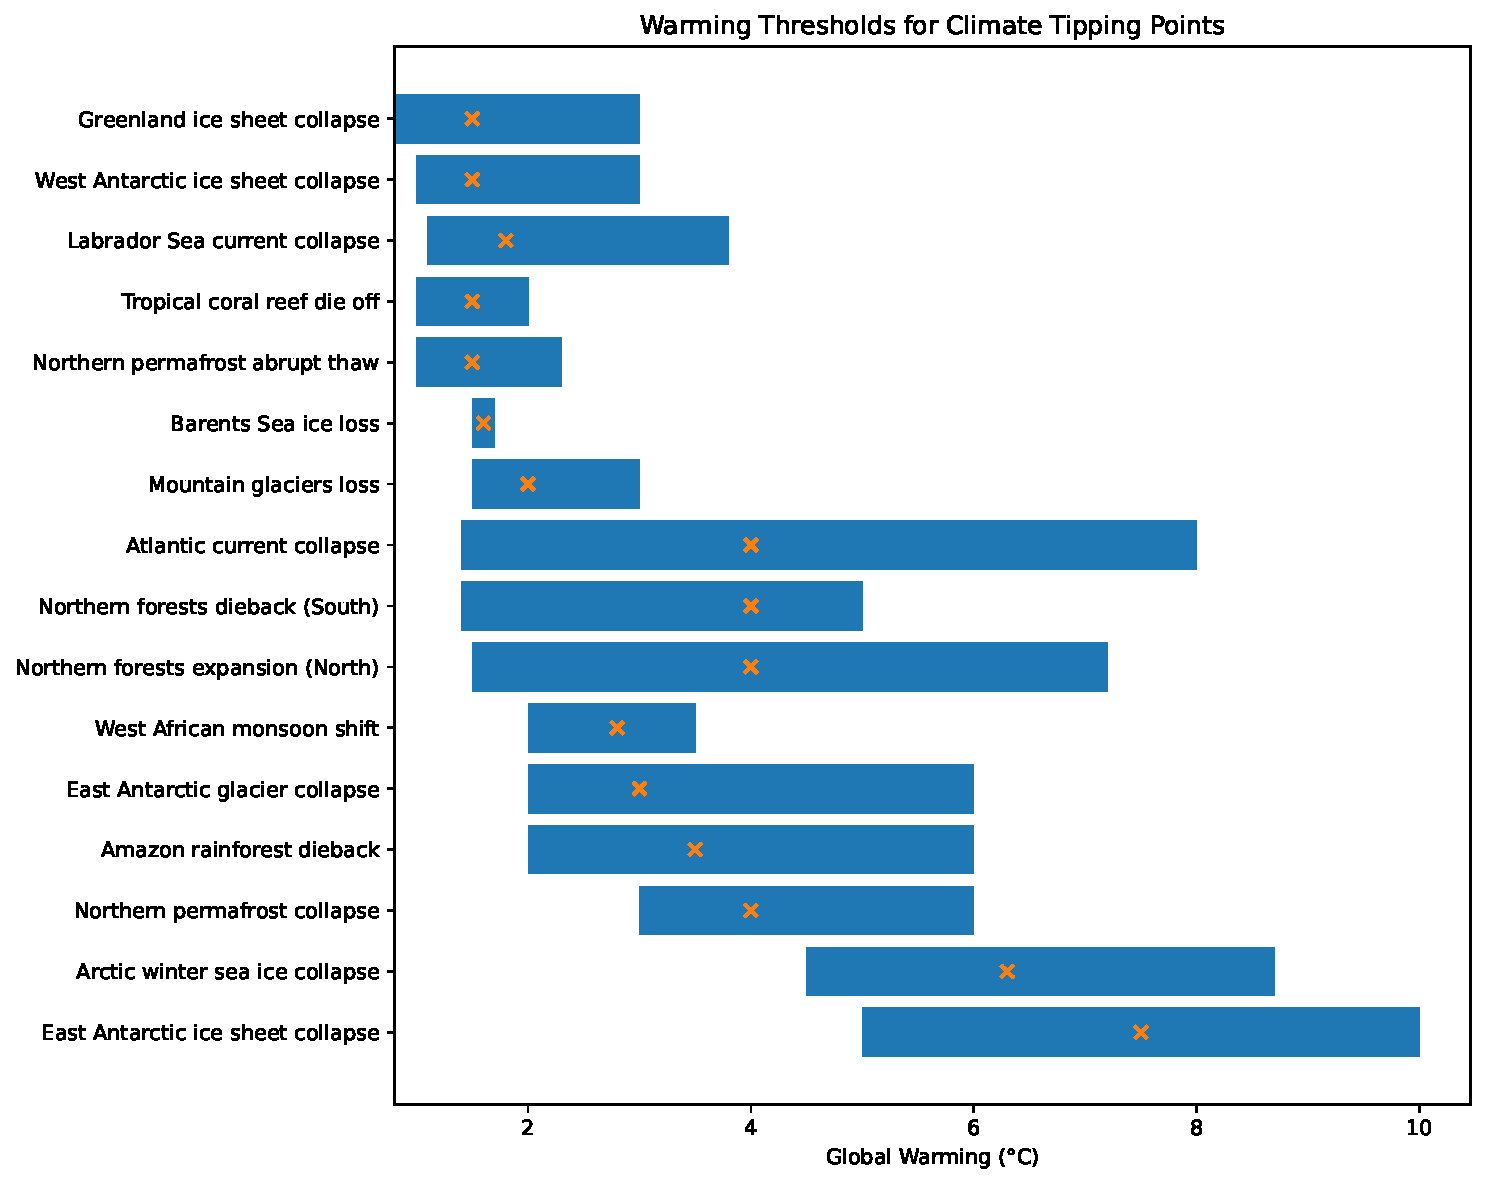
\includegraphics[keepaspectratio]{_thesis_files/figure-pdf/fig-climate-tip-output-1.pdf}}

}

\caption[Climate Tipping Points]{\label{fig-climate-tip}Climate Tipping
Points}

\end{figure}%

\subsubsection{\texorpdfstring{Measuring CO\textsubscript{2}e
Emissions}{Measuring CO2e Emissions}}\label{measuring-co2e-emissions}

Technology improves and measurements have become more accurate yet
CO\textsubscript{2}e emissions are not yet completely accounted for.
(Crippa et al., 2020) reports the latest figures CO\textsubscript{2}e
from the EU's Emissions Database for Global Atmospheric Research
(EDGAR). The EU Copernicus satellite system reveals new greenhouse
emissions previously undetected (Daniel Värjö, 2022). \emph{Copernicus
Climate Change Service (C3S) provides ``{[}n{]}ear-real time updates of
key global climate variables}''(The Copernicus Climate Change Service,
2024). Using simple python code and freely available images from online
datasets, it's increasingly possible for anyone to detect deforestation,
as in this example of geospatial analysis from Amazon AWS (AWS, 2022; P.
Patel, 2025).

One major cross-cutting category the IPCC tracks separately is LULUCF
(Land Use, Land-Use Change, and Forestry). Depending on whether forests
are being cleared or restored, LULUCF can act as a net greenhouse-gas
source or as a powerful carbon sink that removes CO\textsubscript{2}
from the atmosphere. LULUCF also links to biodiversity protection. (Y.
Chen et al., 2023) looked at the Poyang Lake in China between 2010-2020,
finding ecosystem vulnerability rose by 18\% with human activities
(land-use change, urban expansion, components of LULUCF, also reported
in international media, see (Scarr \& Sharma, 2021) for images) as the
dominant driver, followed by climate factors. (Xie et al., 2021) mapped
pollution sources in 14 vulnerable areas in China, including the Poyang
Lake, and underlined the need for real-time monitoring of ecosystem
health.

Emissions production is highly unequal, with \emph{``{[}t{]}he world's
top 1\% of emitters produce over 1000 times more CO\textsubscript{2}eq
than the bottom 1\%''} (IEA, 2023a). The share of CO\textsubscript{2}
emissions among people around the world is highly unequal across the
world (referred to as \emph{Carbon Inequality}). (Chancel, 2022) reports
``one-tenth of the global population is responsible for nearly half of
all emissions, half of the population emits less than 12\%''.
Information and communications technology (ICT) sector is an example of
carbon inequality, where emerging economies bear 82\% of the emissions,
developed countries gain 58\% of value, of the over 300 million PCs sold
per year (Bajarin, 2022; X. Zhou et al., 2022).

CO\textsubscript{2}e emissions by region (per year), comparing highest
per capita CO\textsubscript{2e} emissions (mostly from oil producers) vs
regional average per capita CO\textsubscript{2} emissions vs total
CO\textsubscript{2} emissions.

\def\pandoctableshortcapt{Regional CO\textsubscript{2} Emissions
Comparison}

\begin{longtable}[]{@{}
  >{\raggedright\arraybackslash}p{(\linewidth - 4\tabcolsep) * \real{0.3889}}
  >{\raggedright\arraybackslash}p{(\linewidth - 4\tabcolsep) * \real{0.3194}}
  >{\raggedright\arraybackslash}p{(\linewidth - 4\tabcolsep) * \real{0.2917}}@{}}
\caption[Regional CO~2~ Emissions Comparison]{CO\textsubscript{2}
Emissions Comparison (Crippa et al., 2020; European Commission. Joint
Research Centre., 2022; Ivanova et al., 2020; Z. Liu et al., 2023; World
Resources Institute, 2020).}\tabularnewline
\toprule\noalign{}
\endfirsthead
\endhead
\bottomrule\noalign{}
\endlastfoot
\textbf{Regional Average Per Capita Emissions (2020)} & \textbf{Highest
Per Capita Emissions (2021)} & \textbf{Highest Total Emissions
(2021)} \\
North America 13.4 CO\textsubscript{2}e tonnes & Palau & China \\
Europe 7.5 CO\textsubscript{2}e tonnes & Qatar & United States \\
Global Average 4.1 CO\textsubscript{2}e tonnes & Kuwait & European
Union \\
Africa and the Middle East 1.7 CO\textsubscript{2}e tonnes & Bahrain &
India \\
& Trinidad and Tobago & Russia \\
& New Caledonia & Japan \\
& United Arab Emirates & Iran \\
& Gibraltar & Germany \\
& Falkland Islands & South Korea \\
& Oman & Indonesia \\
& Saudi Arabia & Saudi Arabia \\
& Brunei Darussalam & Canada \\
& Canada & Brazil \\
& Australia & Turkey \\
& United States & South Africa \\
\end{longtable}

\let\pandoctableshortcapt\relax

\emph{Scoping} CO\textsubscript{2e} \emph{emissions} into 4 main
categories helps to organize calculating CO\textsubscript{2e} emissions
and corresponding reduction targets by looking at direct and indirect
emissions separately. The U.S. National Public Utilities Council (NPUC)
decarbonization report provides a useful categorization of
\emph{emission scopes} applicable to companies which helps organizing
emission reduction schemes (National Public Utilities Council, 2022)
based on the Greenhouse Gas Protocol defined in the 1990s (GHG Protocol,
n.d.). For example, for consumers in Australian states and territories
in 2018, 83\% of the GHG emissions are Scope 3, meaning indirect
emissions in the value chain (Goodwin et al., 2023). A newer concept is
Scope 4 emissions also known as avoided emissions, proposed by the World
Resources Institute (WRI) in 2013 (Plan A, n.d.).

\def\pandoctableshortcapt{Definition of Emission Scopes}

\begin{longtable}[]{@{}ll@{}}
\caption[Definition of Emission Scopes]{Definition of Emission Scopes
From (National Public Utilities Council, 2022). One's scope 3 emissions
are someone else's scope 1 emissions.}\tabularnewline
\toprule\noalign{}
\endfirsthead
\endhead
\bottomrule\noalign{}
\endlastfoot
Emission Scope & Emission Source \\
Scope 1 & Direct emissions \\
Scope 2 & Indirect electricity emissions \\
Scope 3 & Value chain emissions \\
Scope 4 & Avoided emissions \\
\end{longtable}

\let\pandoctableshortcapt\relax

Countries have agreed up CO\textsubscript{2e} Reduction Targets known as
Country-Level Nationally Determined Contributions (NDCs). While most
countries have not reached their Nationally Determined Contributions,
the Climate Action Tracker data portal allows to compare countries by
their NDC performance (Climate Analytics \& NewClimate Institute, 2023).
(Fransen et al., 2022) notes that the majority of Nationally Determined
Contributions (NDCs) are dependent on financial assistance from the
international community.

\def\pandoctableshortcapt{Top Polluters}

\begin{longtable}[]{@{}ll@{}}
\caption[Top Polluters]{Climate Action Tracker's country comparison of
the 10 top polluters' climate action (Climate Analytics \& NewClimate
Institute, 2023).}\tabularnewline
\toprule\noalign{}
\endfirsthead
\endhead
\bottomrule\noalign{}
\endlastfoot
Country or Region & NDC target \\
China & Highly insufficient \\
Indonesia & Highly insufficient \\
Russia & Critically insufficient \\
EU & Insufficient \\
USA & Insufficient \\
United Arab Emirates & Highly insufficient \\
Japan & Insufficient \\
South Korea & Highly insufficient \\
Iran & Critically insufficient \\
Saudi Arabia & Highly insufficient \\
\end{longtable}

\let\pandoctableshortcapt\relax

\begin{figure}

\centering{

\pandocbounded{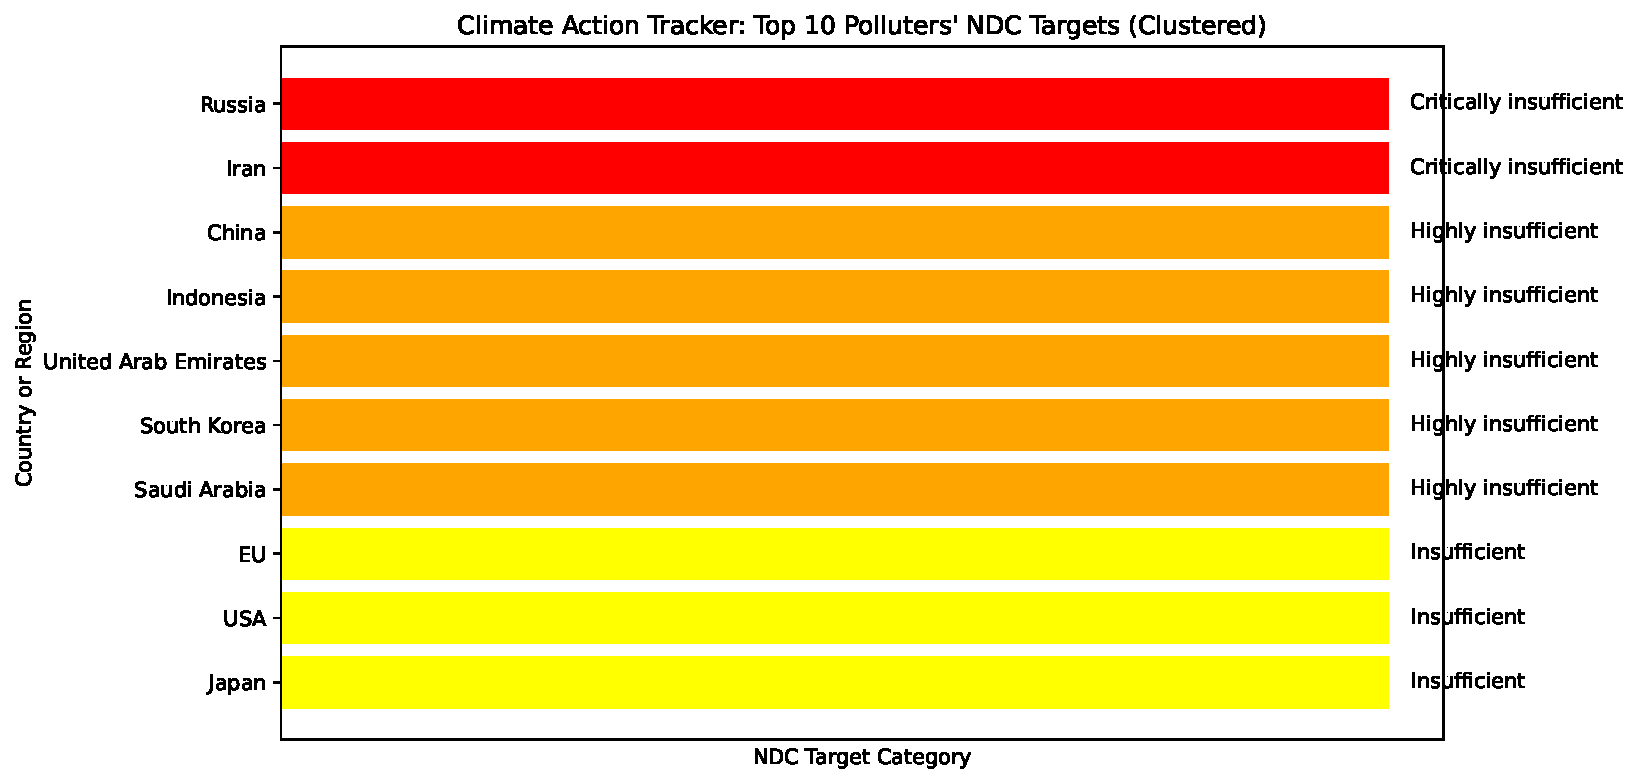
\includegraphics[keepaspectratio]{_thesis_files/figure-pdf/fig-ndcs-output-1.pdf}}

}

\caption[Nationally Determined Contributions
(NDCs)]{\label{fig-ndcs}Nationally Determined Contributions (NDCs)}

\end{figure}%

Fossil fuels are what powers humanity as well as the largest source of
CO\textsubscript{2} emissions. (IEA, 2022) reports ``Global
CO\textsubscript{2} emissions from energy combustion and industrial
processes rebounded in 2021 to reach their highest ever annual level. A
6\% increase from 2020 pushed emissions to 36.3 gigatonnes''. As on June
2023, fossil fuel based energy makes up 82\% of energy and is still
growing (Institute, 2023). The 425 largest fossil fuel projects
represent a total of over 1 gigatons in CO\textsubscript{2} emissions,
40\% of which were new projects Kühne et al. (2022). Tilsted et al.
(2023) expects the fossil fuel industry to continue grow even faster. In
July 2023, the U.K. granted hundreds of new oil and gas of project
licenses in the North Sea ({``Rishi {Sunak} to Green-Light Hundreds of
New Oil and Gas Licenses in {North Sea},''} 2023).

(Ember, 2025) Ember's Electricity Data Explorer shows Taiwanese energy
usage based on data from Taiwanese government, visualizing the growth in
gas, wind, and solar, and decline of coal and nuclear power; however,
while declining, coal remains the leading power source for Taiwan.
Climate pledges made by international companies present in Taiwan mean
they need large amounts of green energy to meet their sustainability
goals. For instance, Google worked with the government of Taiwan to
change the laws to allow direct power procurement by foreign companies;
the current plan being to install 1 gigawatt of solar power fully
pre-purchased by the newly formed company created by BlackRock and
Google for boosting AI development as reported by (S. Chiang, 2024;
Jessop et al., 2024; 永鑫能源 New Green Power, 2022). More recently,
Google also purchased 10MW of geothermal energy for its Taiwanese AI
chip projects, doubling current Taiwanese geothermal capacity
(Hagström-Ilievska, Apr. 17, 2025 18:00; Potter, 2025; Jeffery Wu \&
Thompson, 2025). Geothermal energy provides 24/7 clean energy from the
Earth's core, however is limited due to lack of access; Taiwan happens
to be in geologically active spot on the ring of fire, where drilling
for geothermal energy is more feasible (M. Chang \& Hsiao, 2025; L,
2025b).

\subsubsection{Carbon Accounting, Emissions Trading
Schemes}\label{carbon-accounting-emissions-trading-schemes}

Trading CO\textsubscript{2e} emissions can be divided into 2 categories,
namely \emph{Compliance Carbon Markets} (CCM) and \emph{Voluntary Carbon
Markets} (VCM). The legislative baseline for Compliance Carbon Markets
is so low, people want to retire more CO\textsubscript{2e}, which they
can do through \emph{Voluntary Carbon Markets.}

As of 2024 there's no single global CO\textsubscript{2} trading market
but rather several local markets as described in the table below. Most
of the world is not part of a CO\textsubscript{2} market.

\def\pandoctableshortcapt{CO\textsubscript{2} Credit Trading Markets}

\begin{longtable}[]{@{}
  >{\raggedright\arraybackslash}p{(\linewidth - 4\tabcolsep) * \real{0.2639}}
  >{\raggedright\arraybackslash}p{(\linewidth - 4\tabcolsep) * \real{0.2639}}
  >{\raggedright\arraybackslash}p{(\linewidth - 4\tabcolsep) * \real{0.4722}}@{}}
\caption[CO~2~ Credit Trading Markets]{CO\textsubscript{2} credit
trading markets around the world from (\emph{International Carbon
Market}, n.d.).}\tabularnewline
\toprule\noalign{}
\endfirsthead
\endhead
\bottomrule\noalign{}
\endlastfoot
CO\textsubscript{2} Market & Launch Date & Comments \\
EU & 2005 & EU: (Araújo et al., 2020) \\
South Korea & 2015 & \\
China & 2021 & China's national emissions trading scheme (ETS) started
in 2021 priced at 48 yuan per tonne of CO\textsubscript{2}, averaged at
58 yuan in 2022 (Ivy Yin, 2023; H. Liu, 2021). \\
U.S. & 2013 & No country-wide market; local CO\textsubscript{2} markets
in California, Connecticut, Delaware, Maine, Maryland, Massachusetts,
New Hampshire, New York, Rhode Island, and Vermont \\
New Zealand & 2008 & New Zealand (Rontard \& Reyes Hernández, 2022)
(need access, important NCKU doesn't subscribe) \\
Canada & 2013 & \\
\end{longtable}

\let\pandoctableshortcapt\relax

The price of CO\textsubscript{2e} differs across markets, as assigning a
monetary value to reducing CO\textsubscript{2e} emissions depends on
several variables. (Stern, 2022b) argues carbon-neutral economy needs
higher CO\textsubscript{2e} prices and believes (Rennert et al., 2022)
CO\textsubscript{2e} price per ton should be 3,6x higher that it is
currently. Contrary, (Ritz, 2022) argues optimal CO\textsubscript{2}
prices could be highly asymmetric, low in some countries and high (above
the social cost of CO\textsubscript{2e}) in countries where production
is very polluting. The total size of carbon markets reached 949 billion
USD in 2023, including Chinese, European, and North American
CO\textsubscript{2} trading (LSEG \& Susanna Twidale, 02/12/2024, 02:37
PM).

The prices between compliance and voluntary markets differ
substantially.

\def\pandoctableshortcapt{Compliance Market CO\textsubscript{2} Prices}

\begin{longtable}[]{@{}ll@{}}
\caption[Compliance Market CO~2~ Prices]{Compliance market
CO\textsubscript{2} prices on August 12, 2023; data from (CarbonCredits,
2023; Ember, 2023; Trading Economics, 2023).}\tabularnewline
\toprule\noalign{}
\endfirsthead
\endhead
\bottomrule\noalign{}
\endlastfoot
Compliance Carbon Markets & Price (Tonne of CO\textsubscript{2}) \\
EU & 83 EUR \\
UK & 40 Pounds \\
US (California) & 29 USD \\
Australia & 32 USD \\
New Zealand & 50 USD \\
South Korea & 5.84 USD \\
China & 8.29 USD \\
\end{longtable}

\let\pandoctableshortcapt\relax

\def\pandoctableshortcapt{Voluntary Market CO\textsubscript{2} Prices}

\begin{longtable}[]{@{}ll@{}}
\caption[Voluntary Market CO~2~ Prices]{Voluntary market
CO\textsubscript{2} prices on August 12, 2023; data from (CarbonCredits,
2023).}\tabularnewline
\toprule\noalign{}
\endfirsthead
\endhead
\bottomrule\noalign{}
\endlastfoot
Voluntary Carbon Markets & Price (Tonne of CO\textsubscript{2}) \\
Aviation Industry Offset & \$0.93 \\
Nature Based Offset & \$1.80 \\
Tech Based Offset & \$0.77 \\
\end{longtable}

\let\pandoctableshortcapt\relax

\begin{figure}

\centering{

\pandocbounded{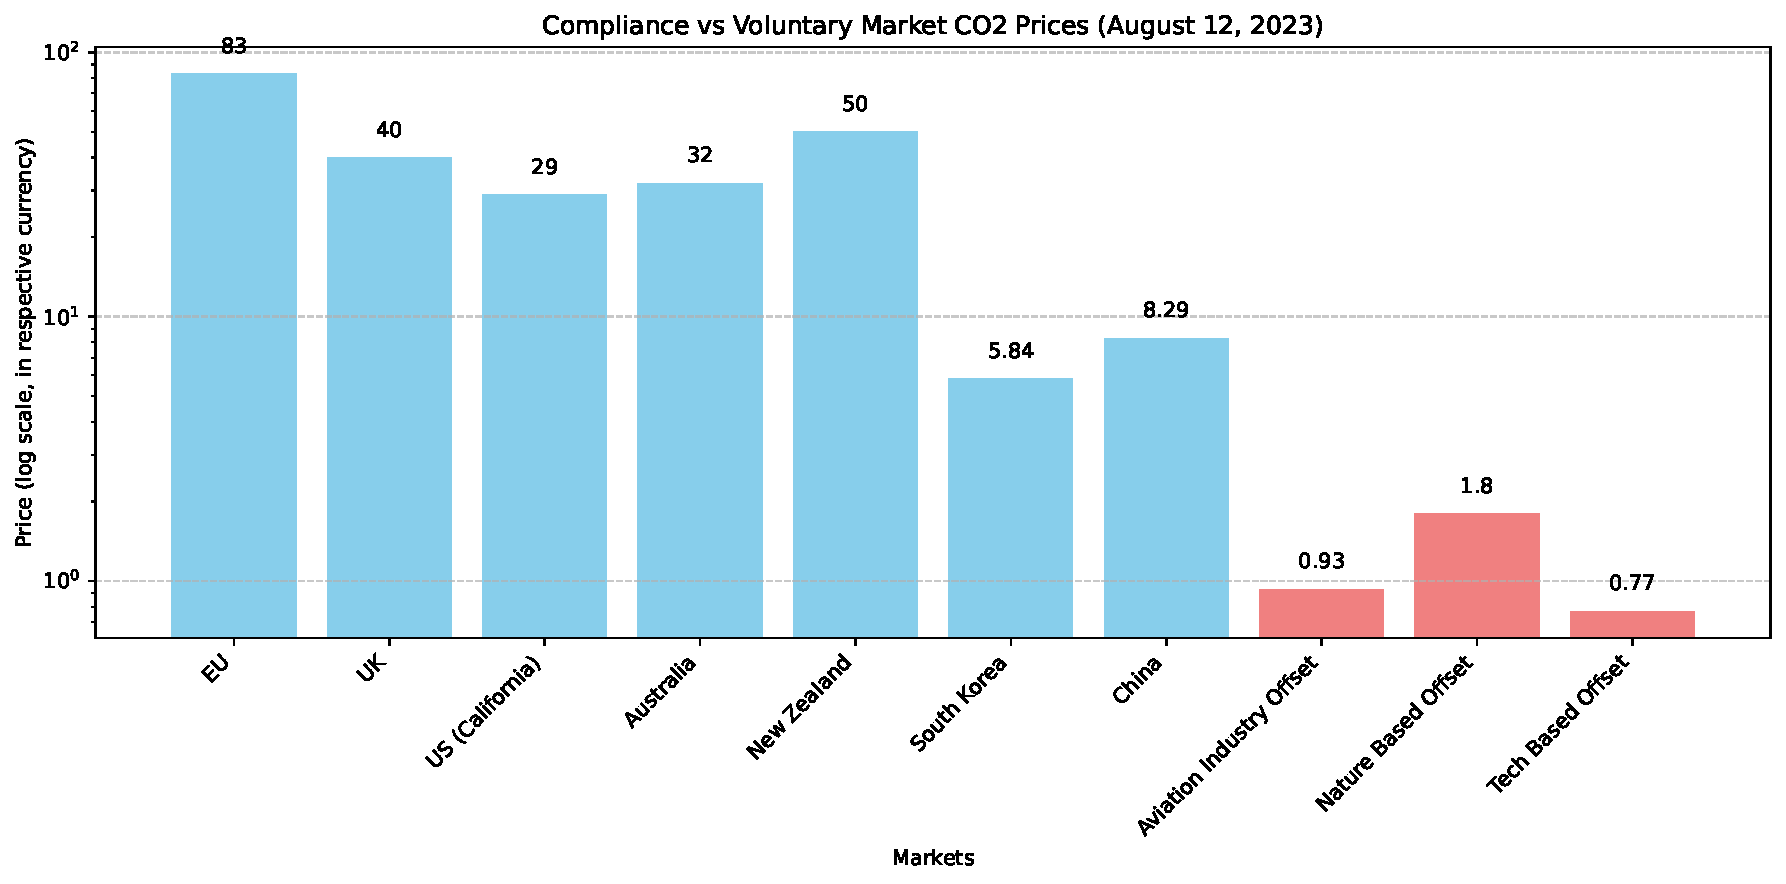
\includegraphics[keepaspectratio]{_thesis_files/figure-pdf/fig-carbon-cred-output-1.pdf}}

}

\caption[Carbon Credits]{\label{fig-carbon-cred}Carbon Credits}

\end{figure}%

Voluntary Carbon Markets are a decentralized system where private
entities voluntarily buy and sell carbon credits (ICVCM, 2025). Carbon
credits are useful for private companies who wish to claim \emph{carbon
neutrality, climate positivity}, or other related claim, which might be
viewed in good light by their clients or allow the companies to adhere
to certain legislative requirements. In the simplest terms, a carbon
credit represents 1T of CO\textsubscript{2}eq that has been prevented
from entering the atmosphere - or has been removed from circulation (aka
Carbon Credit Retirement) (Anna Watson, 2022, 2023). However it's
important to look at the details of these deal as Voluntary Carbon
Markets (VCM) lack standardization and transparency (Ela Khodai, 2023).
For example, Flickr only invested around 3000 USD in carbon credits and
got a carbon-neutral rating, which hardly seems enough for an
organization of its size (Climate Neutral, 2024).

Markets are centered around carbon credits, nature-backed financial
derivatives dependent on science-based methodologies for measurement,
reporting, and verification (MRV), which are managed and regularly
updated by certification organizations such as Gold Standard, Verra, and
others. Some standards released in the past few years include the Verra
Agricultural Land Management methodology for Verified Carbon Standard
(VCS) (Verra, 2023). Gold Standard recently release a methodology for
Mangrove-based carbon credits (Gold Standard, 2024). Regen Network
released a methodology for regenerative grazing systems, proposing
remote-sensing analysis with field-sampled soil carbon data, quantifying
GHG sequestration and ecological co-benefits (biodiversity,
water-infiltration, etc.) for robust MRV and carbon-credit issuance
(\emph{Methodology for {GHG} \& {Co-Benefits} in {Grazing Systems}},
2022). KlimaDAO, unhappy with the current standards, published ``An open
call for alternative carbon standards'' inviting carbon-credit issuers
and communities to propose next-generation registry frameworks and
leverage blockchain for transparency, liquidity and interoperability in
the voluntary carbon market (KlimaDAO, 2023a).

\def\pandoctableshortcapt{Criteria for Carbon Credit Projects}

\begin{longtable}[]{@{}
  >{\raggedright\arraybackslash}p{(\linewidth - 2\tabcolsep) * \real{0.5000}}
  >{\raggedright\arraybackslash}p{(\linewidth - 2\tabcolsep) * \real{0.5000}}@{}}
\caption[Criteria for Carbon Credit Projects]{Criteria for carbon credit
projects from (Verra, 2023).}\tabularnewline
\toprule\noalign{}
\begin{minipage}[b]{\linewidth}\raggedright
Criteria
\end{minipage} & \begin{minipage}[b]{\linewidth}\raggedright
Description
\end{minipage} \\
\midrule\noalign{}
\endfirsthead
\toprule\noalign{}
\begin{minipage}[b]{\linewidth}\raggedright
Criteria
\end{minipage} & \begin{minipage}[b]{\linewidth}\raggedright
Description
\end{minipage} \\
\midrule\noalign{}
\endhead
\bottomrule\noalign{}
\endlastfoot
Baseline & Ecosystem carbon sequestration rate without the intervention
(project) \\
Additionality & New carbon capture or prevention of emissions \\
Permanence & Carbon storage time (should be long-term) \\
Leakage & Risk of shift to causing emissions (for example because of
deforestation) \\
\end{longtable}

\let\pandoctableshortcapt\relax

For the individual person, there's no direct access to
CO\textsubscript{2} markets. However, brokers do buy large amounts of
carbon credits to resell in smaller quantities to retail investors.
Facilitating citizens' access to CO\textsubscript{2} emissions trading
may be an efficient method to organize large-scale CO\textsubscript{2}
retiring (Rousse, 2008). (Sipthorpe et al., 2022) compares traditional
and blockchain-based solutions to carbon trading, arguing that
blockchain solutions for CO\textsubscript{2}eq markets are nearing
maturity, and offer many improvements, such as enhancing transparency,
trust, and efficiency.

CO\textsubscript{2e} credits have given rise to the Carbon Accounting
industry, to help companies meet legal emissions reduction targets in
Compliance Carbon Markets, with many companies like Watershed, Greenly,
and Sustaxo providing services. (Quatrini, 2021) admits sustainability
assessments are often complex and may give flawed results. Nonetheless,
CO\textsubscript{2} emission reduction has the added positive effect of
boosting corporate morale (J. Cao et al., 2023).

There are many companies which facilitate buy carbon credits as well as
a few organizations focused on carbon credit verification. In Estonia,
startups Arbonic and Single.Earth are trialing this approach in several
forests. The most established certifiers or carbon credits include the
Verified Carbon Standard (VCS), the Gold Standard, Climate Action
Reserve (CAR)‍, and the American Carbon Registry (ACR).

\emph{``Carbon pricing is not there to punish people,''} says Lion Hirth
(Lion Hirth, n.d.). \emph{``It's there to remind us, when we take
travel, heating, consumption decisions that the true cost of fossil
fuels comprises not only mining and processing, but also the damage done
by the CO\textsubscript{2} they release.''} Long term cost of
insufficient climate action is more than short-term gains from delaying
efforts to reduce carbon emissions. In addition to the damages from
global warming, the fossil energy production that's a large part of
global CO\textsubscript{2}eq emissions has caused several high-profile
pollution events. Large ones that got international news coverage
include Exxon Valdez and Deepwater Horizon.

Carbon credit prices should reflect the quality of the carbon reduction.
Nature-based carbon removal solutions (for example, forest-backed carbon
credits) rank among the top solutions for mitigating climate change but
require price signals that reflect their true value; Pachama's (an
AI-based carbon removal company) calculation from bottom up cost
modeling across more than 150 reforestation projects indicate that high
quality forest carbon removal credits must trade at a minimum of USD
50-82 per tonne of CO\textsubscript{2}eq to be competitive with
alternative land uses (IPCC AR6 guidance sets the price spread wider,
from USD 50-200); reduced land-use change (basically this means not
cutting down forests, IPCC groups together as LULUCF, Land Use, Land-Use
Change and Forestry) ranks 2nd to solar energy in terms of carbon
reduction potential (Luik, 2025; Pachama, 2023).

\subsubsection{Markets Financialize the Natural World: Pricing, Tracing,
and Trading Ecosystem Services and Nature-backed
Assets}\label{markets-financialize-the-natural-world-pricing-tracing-and-trading-ecosystem-services-and-nature-backed-assets}

Similarly to carbon markets, markets for nature-backed assets and
ecosystem services are centered around different types of credits.

\def\pandoctableshortcapt{Types of Nature-Backed Assets and Tradeable
Ecosystem Services}

\begin{longtable}[]{@{}
  >{\raggedright\arraybackslash}p{(\linewidth - 2\tabcolsep) * \real{0.3194}}
  >{\raggedright\arraybackslash}p{(\linewidth - 2\tabcolsep) * \real{0.6806}}@{}}
\caption[Types of Nature-Backed Assets and Tradeable Ecosystem
Services]{Types of nature-backed assets and tradeable ecosystem services
(Borges et al., 2022; Deloitte, 2024; Fiegenbaum, 2024; PWC, 2025;
Rossberg et al., 2024; U.S. Securities and Exchange Commission,
2023)}\tabularnewline
\toprule\noalign{}
\begin{minipage}[b]{\linewidth}\raggedright
\textbf{Asset Type}
\end{minipage} & \begin{minipage}[b]{\linewidth}\raggedright
\textbf{Description}
\end{minipage} \\
\midrule\noalign{}
\endfirsthead
\toprule\noalign{}
\begin{minipage}[b]{\linewidth}\raggedright
\textbf{Asset Type}
\end{minipage} & \begin{minipage}[b]{\linewidth}\raggedright
\textbf{Description}
\end{minipage} \\
\midrule\noalign{}
\endhead
\bottomrule\noalign{}
\endlastfoot
Carbon Credits and Offsets & Represent avoided or removed
CO\textsubscript{2}eq emissions through reforestation, soil health
improvements, regenerative farming practices that sequester carbon,
etc \\
Biodiversity Credits & Represent conservation and restoration of species
or ecosystems quantified by some standard or criteria such as provided
by Verra and Gold Standard \\
Water Rights and Wetland Credits & Represent rights to access water or
preserve/restore wetlands which can be traded \\
Conservation Finance Instruments & Represent bonds or funds that protect
forests, coral reefs, or species habitats \\
Natural Asset Companies (NACs) & Represents a SEC-backed structure
allowing public trading of ecosystem ownership rights \\
Tokenized Natural Resources & Represent blockchain-based representations
of nature (e.g., tokenized forest) \\
\end{longtable}

\let\pandoctableshortcapt\relax

\subsubsection{Overconsumption \textgreater{} Earth's
Boundaries}\label{overconsumption-earths-boundaries}

Excessive consumer lifestyle - \emph{overconsumption} - is one of the
main drivers of climate change and environmental destruction, with
\emph{``2/3 of global GHG emissions are directly and indirectly linked
to household consumption, with a global average of about 6 tonnes
CO\textsubscript{2} equivalent per capita''} , according to (Ivanova et
al., 2020; Renee Cho, 2020). An older study put the number as high as
60\% percent (Ivanova et al., 2016) while (Ellen MacArthur Foundation,
Material Economics, 2019)'s models 45\% show of CO\textsubscript{2}
equivalent emissions come from our shopping; produced by companies to
make the products we consume. (Keeble, 1988) reported in April 1987 that
\emph{`residents in high-income countries lead lifestyles incompatible
with planetary boundaries'}. (Ivanova et al., 2020) reports the average
footprint in North America and Europe is 13.4 t CO\textsubscript{2}eq,
in Africa and the Middle East 1.7t CO\textsubscript{2}eq; consumption
options with a high mitigation potential measured in tonnes of
CO\textsubscript{2} equivalent per capita per year include
\emph{``living car-free''} and avoiding flying, which could each save
upwards of 1.7t CO\textsubscript{2}eq per person annually.

While the numbers on overconsumption are clear, the debate on
overconsumption is so polarized, it's difficult to have a meaningful
discussion of the topic (Ianole \& Cornescu, 2013). Environmental risks
from human activities are known as Anthropogenic Threat Complexes (ATCs)
(Bowler et al., 2020). With the trend of urbanization, it's not
surprising (people living in) cities are responsible for 80\% of the
emissions (Rosales Carreón \& Worrell, 2018). (Moberg et al., 2019)
reports daily human activities emission contribution on average in four
European countries (France, Germany, Norway and Sweden).

\def\pandoctableshortcapt{Daily Human Activities' Emission Contribution}

\begin{longtable}[]{@{}ll@{}}
\caption[Daily Human Activities' Emission Contribution]{Daily human
activities emission contribution on average in France, Germany, Norway
and Sweden from (Moberg et al., 2019).}\tabularnewline
\toprule\noalign{}
\endfirsthead
\endhead
\bottomrule\noalign{}
\endlastfoot
Emission Share & Category \\
21\% & Housing \\
30\% & Food \\
34\% & Mobility \\
15\% & Other \\
\end{longtable}

\let\pandoctableshortcapt\relax

Taking a broader view, (Hannah Ritchie, 2020; US EPA, 2016) dissect GHG
emissions inventory by sector and put the blame squarely on the type of
energy used.

\def\pandoctableshortcapt{Industrial Emissions}

\begin{longtable}[]{@{}
  >{\raggedright\arraybackslash}p{(\linewidth - 4\tabcolsep) * \real{0.2222}}
  >{\raggedleft\arraybackslash}p{(\linewidth - 4\tabcolsep) * \real{0.2222}}
  >{\raggedright\arraybackslash}p{(\linewidth - 4\tabcolsep) * \real{0.5556}}@{}}
\caption[Industrial Emissions]{Industrial Emissions (Hannah Ritchie,
2020; US EPA, 2016).}\tabularnewline
\toprule\noalign{}
\begin{minipage}[b]{\linewidth}\raggedright
Sector
\end{minipage} & \begin{minipage}[b]{\linewidth}\raggedleft
Share
\end{minipage} & \begin{minipage}[b]{\linewidth}\raggedright
Description
\end{minipage} \\
\midrule\noalign{}
\endfirsthead
\toprule\noalign{}
\begin{minipage}[b]{\linewidth}\raggedright
Sector
\end{minipage} & \begin{minipage}[b]{\linewidth}\raggedleft
Share
\end{minipage} & \begin{minipage}[b]{\linewidth}\raggedright
Description
\end{minipage} \\
\midrule\noalign{}
\endhead
\bottomrule\noalign{}
\endlastfoot
Energy Use (inc. electricity, heat and transport) & 73.2 \% & Total
CO\textsubscript{2}eq emissions from all fuel combustion and related
fugitive losses. Energy use in industry (24.2\%) in processing metals
(iron and steel), chemicals and petrochemicals, food and tobacco, non
ferrous metals, paper, machinery, other industry; transport (16.2\%)
road, aviation, shipping, rail; buildings (17.5\%) including residential
and commercial; fugitive emissions (5.8\%) such as methane leaks from
oil and gas exploitation and coal mining; plus other, unallocated fuel
combustion related emissions (7.8\%) \\
Direct Industrial Processes & 5.2 \% & Direct CO\textsubscript{2}eq
emissions from chemical reactions in cement and in chemicals and
petrochemicals. \\
Waste & 3.2 \% & Wastewater methane and NO2 emissions; landfill
methane. \\
Agriculture + LULUCF (Land Use, Land-Use Change \& Forestry) & 18.4 \% &
Emissions from grassland, cropland, deforestation, crop burning, rice
cultivation, agricultural soils, livestock and manure. \\
\end{longtable}

\let\pandoctableshortcapt\relax

Earth's growing population reached 8 Billion people In November 2022 and
population projections by predict 8.5B people by 2030 and 9.7B by 2050
(The Economic Times, 2022; United Nations Department of Economic and
Social Affairs, Population Division, 2022). Indeed, making
\emph{anything} consumes natural resources, which are limited on planet
Earth. (Hassoun et al., 2023) forecasts increase of global food demand
by 62\% driven by the impact of climate change. Yet, while population
growth puts higher pressure on Earth's resources, some researchers
propose the effect is higher from wasteful lifestyles than the raw
number of people (Cardinale et al., 2012). Meanwhile others, such as
(Cafaro et al., 2022), believe \emph{{[}o{]}verpopulation is a major
cause of biodiversity loss and smaller human populations are necessary
to preserve what is left.''}

\subsubsection{Plastic Pollution}\label{plastic-pollution}

Overconsumption is also one of the root causes of plastic pollution.
(Ford et al., 2022) and (Lavers et al., 2022) find strong links between
climate change and marine plastic pollution \emph{``along with other
stressors that threaten the resilience of species and habitats sensitive
to both climate change and plastic pollution''}.

Plastic pollution is pervasive around the Earth and is fundamentally
linked to climate change, while microplastics are increasingly a real
concern (Lavers et al., 2022; Tiernan et al., 2022). Several
international studies report recent findings of microplastics everywhere
in human bodies: the brain, lungs, digestive tissues, bone marrow,
penis, testis, seminal fluid (semen), and placenta - causing serious
health and reproductive concerns (Codrington et al., 2024; M. A. Garcia
et al., 2024; Guo et al., 2024; Hu et al., 2024; N. Li et al., 2024;
Main, 2024; Montano et al., 2023; L. Zhu et al., 2024)

\begin{figure}

\centering{

\pandocbounded{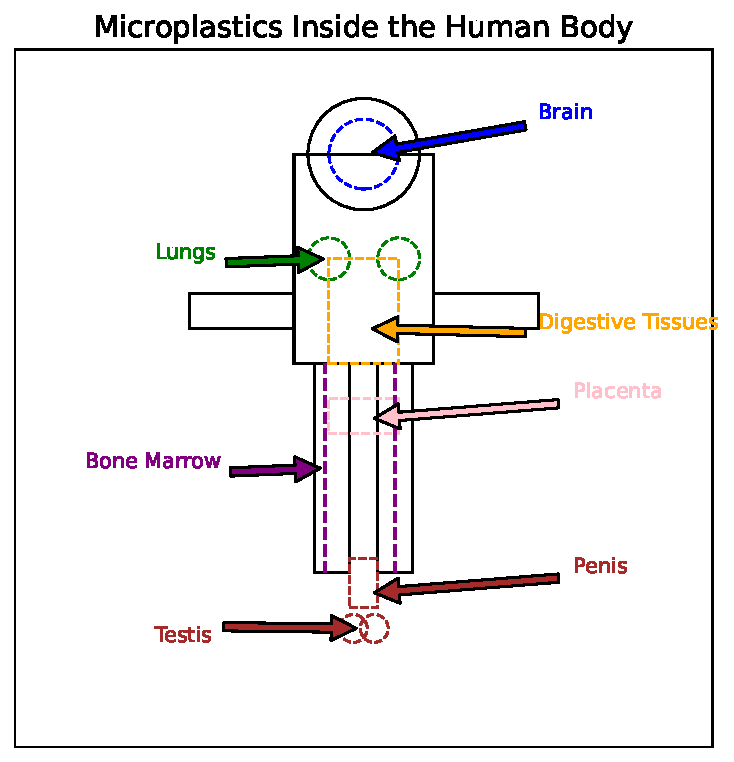
\includegraphics[keepaspectratio]{_thesis_files/figure-pdf/fig-microplastics-output-1.pdf}}

}

\caption[Microplastics in the Human
Body]{\label{fig-microplastics}Microplastics in the Human Body}

\end{figure}%

In addition to the enormity of over-reaching CO\textsubscript{2}
emissions, humanity is facing other massive environmental problems. The
Stockholm Resilience Centre report in 2022 we have already breached 4
out of our 9 \emph{``planetary boundaries'':} in addition to climate
change, biodiversity loss (Extinctions per Million Species per Year aka
E/MSY), land-system change (deforestation, land degradation, etc), and
biogeochemical flows (cycles of carbon, nitrogen, phosphorus, etc); on a
positive side, the challenges of fresh water use, ocean acidification
and stratospheric ozone depletion are still within planetary limits
(Persson et al., 2022).

An update to the planetary boundaries framework a year later found the
actual number to be 6 of 9 boundaries (climate, biosphere integrity,
land use, biogeochemical flows, freshwater use, novel entities) already
transgressed, with ocean acidification nearing its limit and only
stratospheric ozone recovering; atmospheric aerosol loading and the
biodiversity intactness index (BII), which belongs under biodiversity
loss and measures how depleted are the species that are still around
(but not yet extinct), were quantified recently (Newbold et al., 2016;
Richardson et al., 2023).

In the biospehere, mass extinctions are underway. An analysis of
population trends for 27600 terrestrial vertebrate species (including a
detailed sample of 177 mammals), found 32\% (8851 species) are
undergoing severe range contractions; the authors name this ``biological
annihilation'' to signal Earth's ongoing 6 mass extinction and call for
immediate conservation action (Ceballos et al., 2017). As of last year,
the Red List curated by the International Union for Conservation of
Nature (IUCN), includes 45,300 species (28\% of all assessed, since IUCN
was founded in 1948), under threat of extinction (IUCN, 2024).

Responding to the crisis, the Guardian newspaper in the UK has take a
clear stance, covering stories of exctinction; the \emph{Area de
Conservación Guanacaste} is one of the protected areas listed by the
UNESCO World Heritage Centre, providing data on the State of
Conservation (SOC) by year (Centre, 1999; McClure, 2025)

\begin{figure}

{\centering 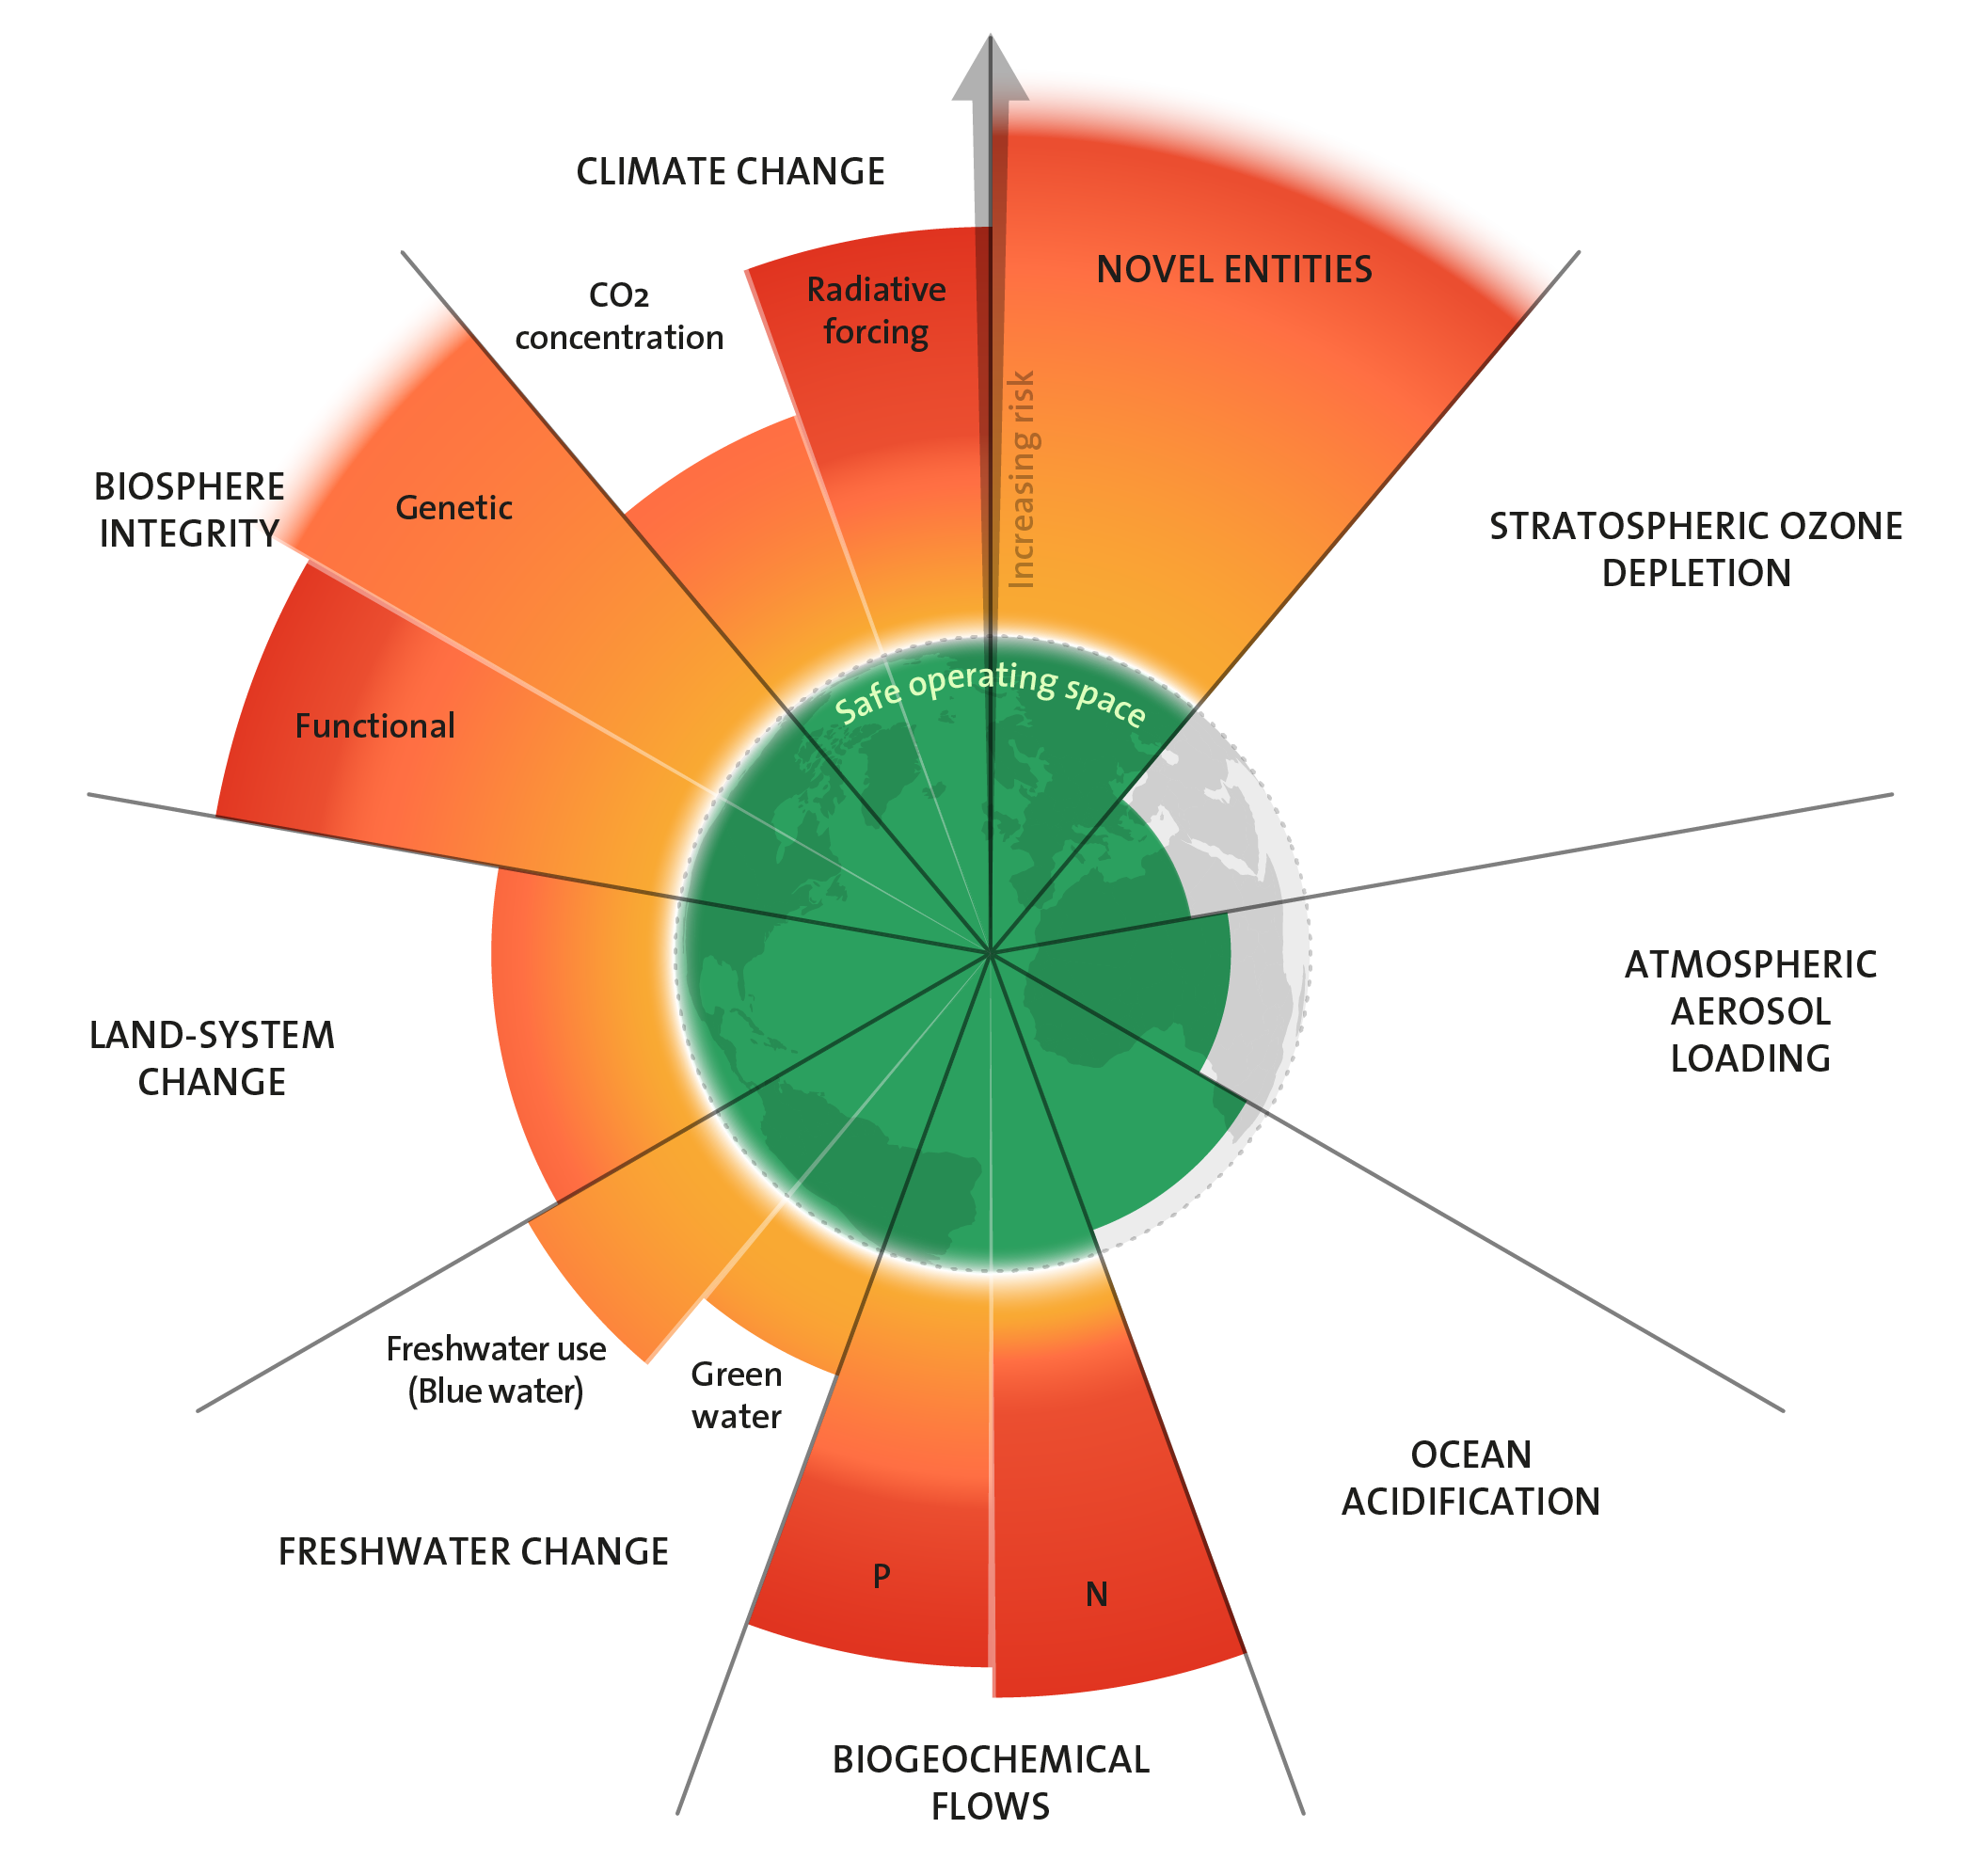
\includegraphics[width=1\linewidth,height=\textheight,keepaspectratio]{./images/sustainability/planetary-boundaries-2023.png}

}

\caption[Planetary Boundaries 2023 Update]{Planetary Boundaries 2023
update. Azote for Stockholm Resilience Centre, based on analysis in
Richardson et al 2023}

\end{figure}%

In 2018 Swedish Sportswear brand Houdini launched the first corporate
planetary boundaries assessment in partnership with Albaeco and
Stockholm Resilience Centre to establish a baseline for its ``impact
positive'' ambition (Houdini, 2018). While it's a pilot study, it
demonstrates how companies can integrate system-level science into
sustainability reporting (Haeggman et al., 2018). At the 2024 update for
the report, Houdini invited, Johan Rockström, a renown conservation and
climate scientist, envisions a global dashboard of the development of
the economy and the state of the planetary boundaries, with high
resolution maps, to help visualize Earth's situation in real-time
(Houdini Sportswear, 2024).

\subsubsection{Evolving Measurements from Planetary Health to Earth
System Law, and Social Cost of
Carbon}\label{evolving-measurements-from-planetary-health-to-earth-system-law-and-social-cost-of-carbon}

Scientists in cross-disciplinary teams have been working on integrating
Earth systems and human society into cohesive frameworks. (Wardani et
al., 2023) stresses that every facet of Earth's life-support
system---living biota and the ``abiotic'' foundations of climate, water,
soils, and geology---co-produces the conditions for civilization:
\emph{``long-term human well-being is dependent on the well-being of the
planet, including both biotic and abiotic systems. It recognizes
interlinkages across environmental sustainability, public health, and
socioeconomic development.''}

There are 3 approaches that address the complex interdependence of
humans with our physical environment, that have the potential to be
complementary - \emph{Planetary Health}, \emph{Social Cost of Carbon},
and \emph{Earth System Law}.

\emph{Planetary Health} is a framework rooted in public health sciences
and medicine; what if public health leveled-up to planetary scale,
concerned with the health of ecological life-support systems: clean air,
food, and a safe climate, so they can support human flourishing; in
practice the framework focuses on evidence, education, governance, and
business (Planetary Health Alliance, 2024a, 2024b).

\emph{Social Cost of Carbon} attempts to measures the compound impact of
CO\textsubscript{2e} emissions on society. Sustainability is filled with
complexities. CO\textsubscript{2e} emissions are complicated by
biodiversity loss, child labor, slavery, poverty, chemical pollution,
etc. - many issues become intertwined (TEDx Talks, 2020). One attempt to
measure these complexities, is the \emph{Social Cost of Carbon} (SCC)
which is defined as \emph{``additional damage caused by an extra unit of
emissions''} (Kornek et al., 2021; Zhen et al., 2018). For example the
cost of damages caused by ``one extra ton of carbon dioxide emissions''
(Stanford University, 2021). SCC variations exist between countries
(Tol, 2019) and regions (Yong Wang et al., 2022).

\emph{Earth System Law} is a framework rooted in the legal sciences for
addressing interconnected environmental challenges in a hyper-connected
Earth, where climate feedbacks and environmental thresholds don't
respect country borders; in practice, this line of thinking helps to
develop carbon-budget clauses inside trade deals and biodiversity
``safety brakes'' that trigger when monitoring data shows an Earth
boundary overshoot, potentially acting as the legal scaffolding that
lets Planetary Health prescriptions and Social Cost of Carbon price
signals be effective (Du Toit \& Kotzé, 2022).

More recently, because of the complex interdependence, (J. Zhang et al.,
2025) proposes a new sustainability index that systematically considers
pertinent indicators of interdependencies and interactions across
different dimensions of sustainability. Moreover, (Lenton et al., 2023)
proposed a new innovative way to quantify the ``cost'' of global warming
in human terms by counting the number of people forced outside the
``human climate niche'' (temperatures historically occupied by most of
humanity); climate change has already exposed ≈9\% of today's population
(\textgreater600 million) unprecedented heat stress, risking increased
mortality, morbidity and displacement; if current trends continue by
2100, \textasciitilde2.7 °C , 21--39 \% or 2--4 billion people will be
exposed by 2080--2100.

\subsection{Quantifying Human Benefits from the Biosphere: Ecosystem
Services}\label{quantifying-human-benefits-from-the-biosphere-ecosystem-services}

\emph{Ecosystem services measure the benefits humans receive from the
biosphere.} Put simply, \emph{ecosystem services} enable human life on
Earth - we are, in a very real sense, - dependent on nature. The
biosphere is Earth's life support system. Earth's biosphere is made up
of 846 terrestrial ecoregions, which are distributed across 14 major
biomes and 8 biogeographical realms (Dinerstein et al., 2017).

While it can be assumed much of the flora and fauna are crucial for
Earth's systems, science is still in the process of understanding and
quantifying its contributions. The history of the valuation of nature's
services goes back to the 18th century when David Ricardo and Jean
Baptiste Say discussed nature's \emph{work}, however both considered it
should be free (Gómez-Baggethun et al., 2010). In 1997 (Daily, 1997)
proposed the idea of \emph{ecosystem services} and (Costanza et al.,
1997) attempted to assess the amount of ecosystem services provided. (Le
Provost et al., 2022)'s study shows \emph{biodiversity} as one key
factor to maintain delivery of ecosystem services. (Noriega et al.,
2018) attempts to quantify the ecosystem services (ES) provided by
insects.

The most complex computer models which attempt to capture ever more
interactions happening in the physical realm are called \emph{digital
twins.} The EU is developing a digital twin of Earth to help
sustainability prediction and planning, integrating Earth's various
systems such as climate, hydrology, ecology, etc, into a single model
(\emph{Destination {Earth} {\textbar} {Shaping Europe}'s Digital
Future}, 2023; J. Hoffmann et al., 2023). For instance, AI is being used
to map icebergs and measure the change in size (European Space Agency,
2023). We can use all the data being recorded to provide a digital twin
of the planet, nature, ecosystems and human actions to help us change
our behavior and optimize for planetary wellbeing.

\subsubsection{Ecological Indicators to Track Environmental
Health}\label{ecological-indicators-to-track-environmental-health}

\subsubsection{Measuring Biodiversity Loss, Ecological Indicators and
Environmental
Degradation}\label{measuring-biodiversity-loss-ecological-indicators-and-environmental-degradation}

Sustainability can be measured using a variety of \emph{ecological
indicators}. Ecological indicators for Earth \emph{- I would like to
coin the word ``ecomarkers'' -} are like \emph{biomarkers} in human
health. Technological advances help scientist better understand nature.
Cutting edge research uses AI-based voice recognition for listening to
nature, assessing biodiversity based on species' sounds in the forest.
Millions of detections of different species with machine learning
passive acoustic AI models, can also assess species' response to climate
change (AI for Good, 2023; Guerrero et al., 2023).

Around the world, pressure on ecosystems is rapidly increasing, with
biodiversity destruction ever prevalent, making protecting biodiversity
as urgent as protecting the climate. (Almond, R.E.A. et al., 2022)
reported, the number of species killed, mass destruction of nature:

\begin{quote}
\emph{``69\% decline in the relative abundance of monitored wildlife
populations around the world between 1970 and 2018. Latin America shows
the greatest regional decline in average population abundance (94\%),
while freshwater species populations have seen the greatest overall
global decline (83\%).''}
\end{quote}

In Europe, as of 2025, none of the evaluated biodiversity targets are on
track; agricultural targets, such as reducing soil nutrient losses, and
reducing fertiliser use, are particularly lagging (European Commission,
2025).

\emph{Environmental DNA (eDNA)} helps scientists measure species
abundance without direct observation through detection of DNA on genetic
materials such as skin cells (Peter Andrey Smitharchive page, 2024).
Cellular DNA can be isolated from various sediment types (Ogram et al.,
1987). Beyond scientific applications, eDNa is being used to generate
biodiversity credits by environmental asset rating companies such as
BeZero, a ratings agency for the Voluntary Carbon Market (Ojoatre \&
Atkinson, 2023).

Similarly to climate protection, the UN has taken a leadership role in
biodiversity protection, by organizing an annual Convention on
Biodiversity. The history of the United Nations Convention on
Biodiversity goes back to 1988, when the working group was founded
(Unit, 2023). The Convention on Biodiversity 2022 (COP15) adopted the
first global biodiversity framework to accompany climate goals (UNEP,
Tue, 12/20/2022 - 07:44).

\def\pandoctableshortcapt{Biodiversity Loss}

\begin{longtable}[]{@{}
  >{\raggedright\arraybackslash}p{(\linewidth - 2\tabcolsep) * \real{0.6111}}
  >{\raggedright\arraybackslash}p{(\linewidth - 2\tabcolsep) * \real{0.3889}}@{}}
\caption[Biodiversity Loss]{Biodiversity loss data from (Bradshaw et
al., 2021).}\tabularnewline
\toprule\noalign{}
\endfirsthead
\endhead
\bottomrule\noalign{}
\endlastfoot
What Happened? & How Much? \\
Vertebrate species population average decline & 68\% over the last 50
years \\
Land surface altered by humans & 70\% of Earth \\
Vertebrate species extinct & 700 in 500 years \\
Plant species extinct & 600 in 500 years \\
Species under threat of extinction & 1 million \\
\end{longtable}

\let\pandoctableshortcapt\relax

\begin{figure}

\centering{

\pandocbounded{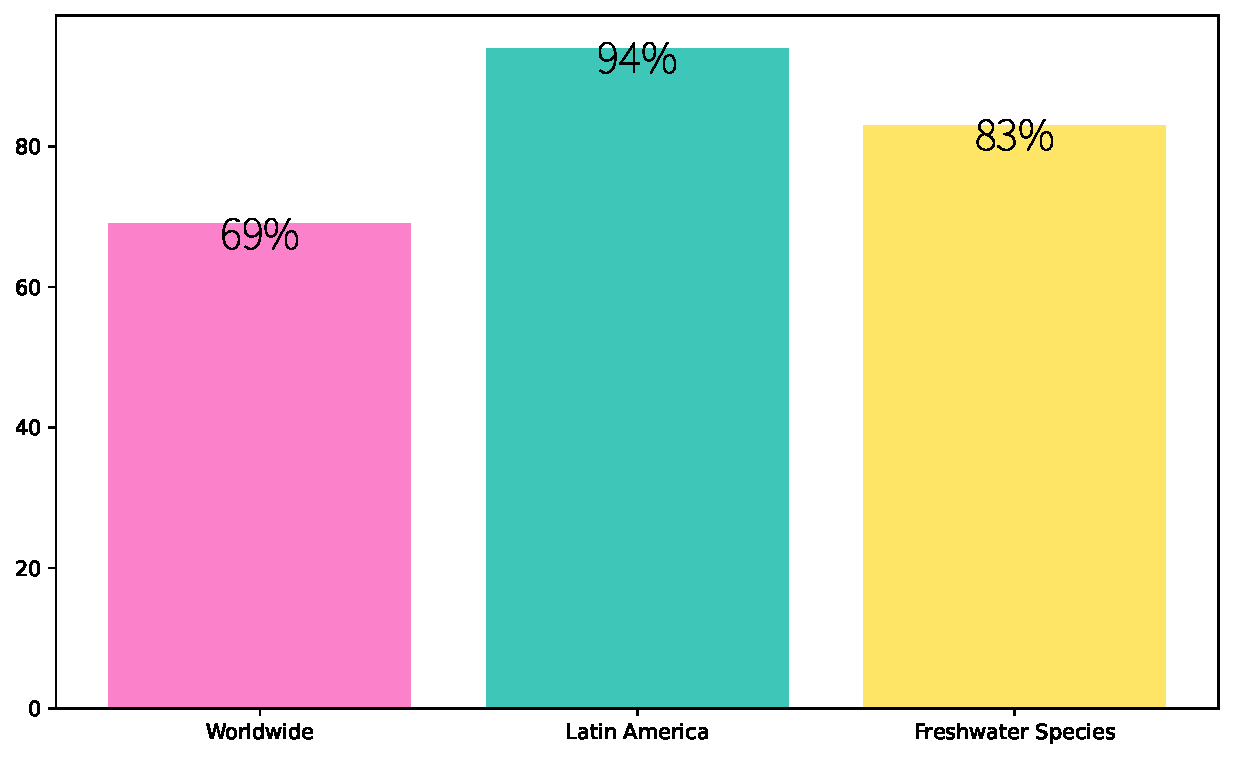
\includegraphics[keepaspectratio]{_thesis_files/figure-pdf/fig-biod-loss-output-1.pdf}}

}

\caption[Biodiversity Loss]{\label{fig-biod-loss}Biodiversity Loss}

\end{figure}%

Biodiversity loss is linked to overconsumption, weak legislation and
lack of oversight. (Crenna et al., 2019) recounts European Union
consumers' negative impact on biodiversity in countries where it imports
food. (WWF, 2022) case study highlights how 4 biodiverse regions Cerrado
in Brazil, Chaco in Argentina, Sumatra in Indonesia, and the Cuvette
Centrale in Democratic Republic of Congo are experiencing rapid
destruction due to consumer demand in the European Union. While the
European Union (EU) has recently become a leader in sustainability
legislation, biodiversity protection measures among private companies is
very low Marco-Fondevila \& Álvarez-Etxeberría (2023).

Starting with the simple question: why protect biodiversity. (May, 2011)
argues biodiversity loss is a concern for 3 points of views:

\def\pandoctableshortcapt{Ethical and Utilitarian Concepts of
Biodiversity Protection}

\begin{longtable}[]{@{}
  >{\raggedright\arraybackslash}p{(\linewidth - 2\tabcolsep) * \real{0.3611}}
  >{\raggedright\arraybackslash}p{(\linewidth - 2\tabcolsep) * \real{0.6389}}@{}}
\caption[Ethical and Utilitarian Concepts of Biodiversity
Protection]{Ethical and Utilitarian Concepts of Biodiversity Protection
from (May, 2011).}\tabularnewline
\toprule\noalign{}
\endfirsthead
\endhead
\bottomrule\noalign{}
\endlastfoot
Point of View & Description \\
Narrowly Utilitarian & Biodiversity is a resource of genetic novelties
for the biotech industry. \\
Broadly Utilitarian & Humans depend upon biodiverse ecosystems. \\
Ethical & Humans have a responsibility to future generations to pass
down a rich natural world. \\
\end{longtable}

\let\pandoctableshortcapt\relax

There is some progress in biodiversity conservation as
``{[}*b{]}iodiversity awareness is now at 72\% or higher in all
countries sampled, compared to only 29\% or higher across countries
sampled in 2009''* (UEBT, 2022)

\subsubsection{Oceans and Marine Ecosystem
Sustainability}\label{oceans-and-marine-ecosystem-sustainability}

Marine heatwaves are intensifying under climate change, threatening
species diversity and the ocean's capacity to supply critical services
from fisheries to carbon sequestration (Smale et al., 2019).
Accelerating ocean warming, evidenced by record-breaking sea-surface
temperatures, has triggered widespread coral bleaching, clearly visible
at the Great Barrier Reef in Queensland, East Coast of Australia, loss
of marine habitat complexity, and cascading threats to coastal economies
and food security; the authors call for integrated climate--ocean policy
action, stressing that without urgent emissions cuts and ecosystem-based
adaptation, the ocean's capacity to regulate climate and sustain
biodiversity will collapse (Gelles \& Andreoni, 2023; Pfeiffer, 2024).
Cumulative pressures: climate extremes, pollution, and overexploitation
- have driven evolutionary shifts in marine life and unpredictably
altered ecosystem-service delivery (Espinosa \& Bazairi, 2023).

Some earlier studies, such as (Howard et al., 2017) demonstrate how
integrating blue carbon habitats into Marine Protected Area (MPA) design
can both mitigate carbon emissions and enhance ecosystem resilience.
Meta-analyses across 121 sites in 87 MPAs globally show that most
well-designed and managed MPAs achieve significant ecological gains: on
average, fish biomass inside no-take zones can double to triple compared
with outside areas, and species richness likewise increases by 20--30 \%
within 5--10 years of enforcement (Rudd, 2015). However, Marine
Protected Areas cover only 8\% of the world's oceans and only 2.8\% is
effectively protected (Igini, 2024a). The UN's 30x30 target (set under
the Convention on Biological Diversity) aims to protect 30\% of the
world's oceans by 2030, however is not on track to achieve this goal
(Mouterde, 2024).

\subsubsection{Forests: Carbon Sinks and Biodiversity
Reservoirs}\label{forests-carbon-sinks-and-biodiversity-reservoirs}

Forests are a crucial part of Earth's carbon cycle and the main natural
CO\textsubscript{2} capture system; due to deforestation, Europe rapidly
losing its forest carbon sink (Frédéric Simon, 2022). Beyond their role
in locking away carbon, recent field work shows forest actively scrub
methane from the air as tree bark absorbs methane (Gauci et al., 2024).
Around 27\% of Earth's land area is still covered by forests yet
\emph{deforestation} is widespread all around the world; highest rates
of deforestation happened in the tropical rainforests of South America
and Africa, mainly caused by agricultural cropland expansion (50\% of
all deforestation) and grazing land for farm animals to produce meat
(38,5\%), totaling close to 90\% of global deforestation (\emph{{FRA}
2020 {Remote Sensing Survey}}, 2022). The global forest cover change is
visible on Google's Earth Engine (Hansen et al., 2013).

Around the world, there are many initiatives to increase forest cover,
for example the \emph{1 billion tree project} (Bastin et al., 2019;
{``Erratum for the {Report},''} 2020; Greenfield \& @pgreenfielduk,
2021). However, it's important to not planting trees
(\emph{afforestation)} is not the full solution, as \emph{afforestation}
is different from \emph{reforestation}, which takes into account
biodiversity. Also, while using remote-sensing and machine-learning to
assess reforestation potential (see Klosterman et al., 2022), it doesn't
take into account local political realities, and socioeconomic issues
such as education, poverty and access to green jobs. Taking these aspect
into account may be beneficial, for example (Bousfield et al., 2022)
reports there's evidence paying landowners for the ecosystem services
their forests provide may reduce deforestation.

\subsubsection{Pollution: Air, Water, and Soil
Degradation}\label{pollution-air-water-and-soil-degradation}

In, Taiwan this is the ranking of pollution reports by citizens
(Ministry of Digital Affairs, 2024b):

\begin{figure}

\centering{

\pandocbounded{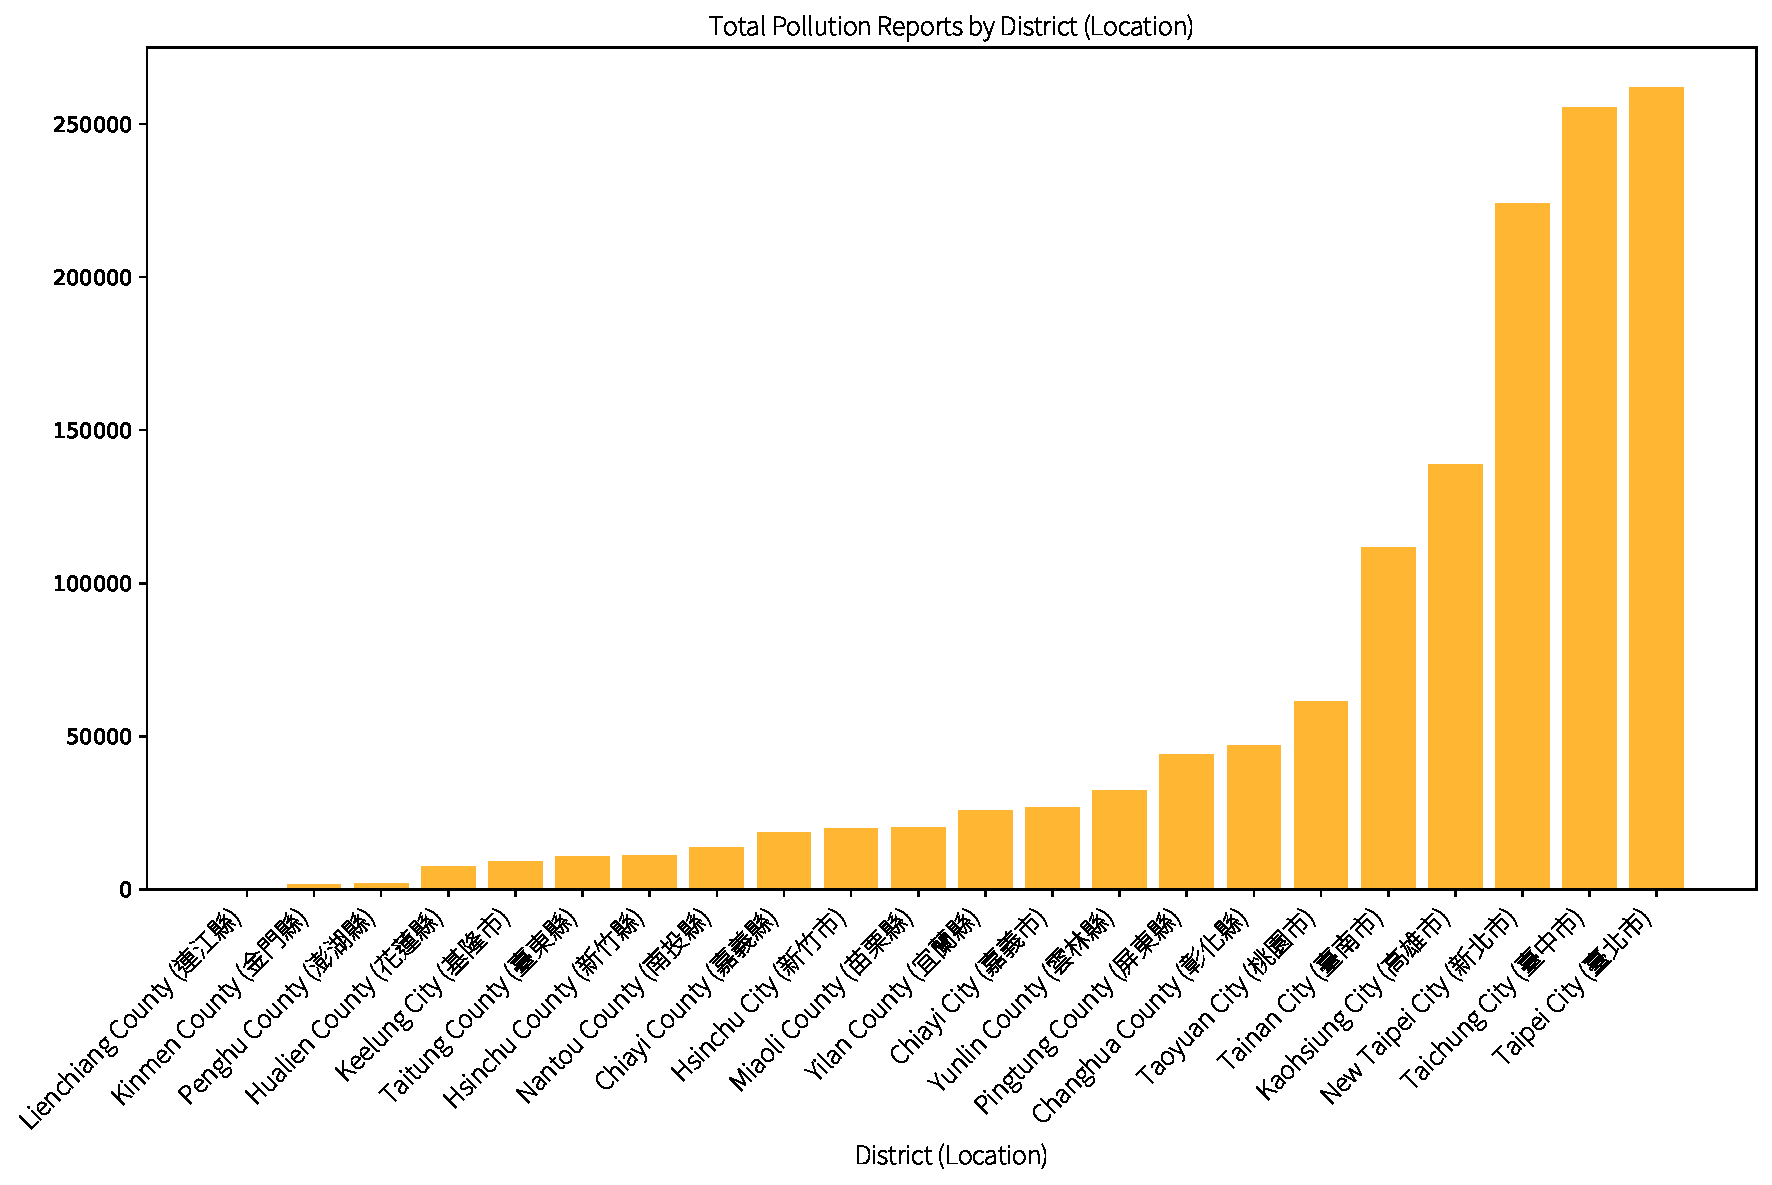
\includegraphics[keepaspectratio]{_thesis_files/figure-pdf/fig-tw-poll-reports-output-1.pdf}}

}

\caption[Pollution Reports in Taiwan by
County]{\label{fig-tw-poll-reports}Pollution Reports in Taiwan by
County}

\end{figure}%

\begin{figure}

\centering{

\centering{

\begin{verbatim}
<Figure size 3600x2400 with 0 Axes>
\end{verbatim}

}

\subcaption{\label{fig-tw-poll-reports-stack-1}Pollution Reports in
Taiwan by District}

\centering{

\pandocbounded{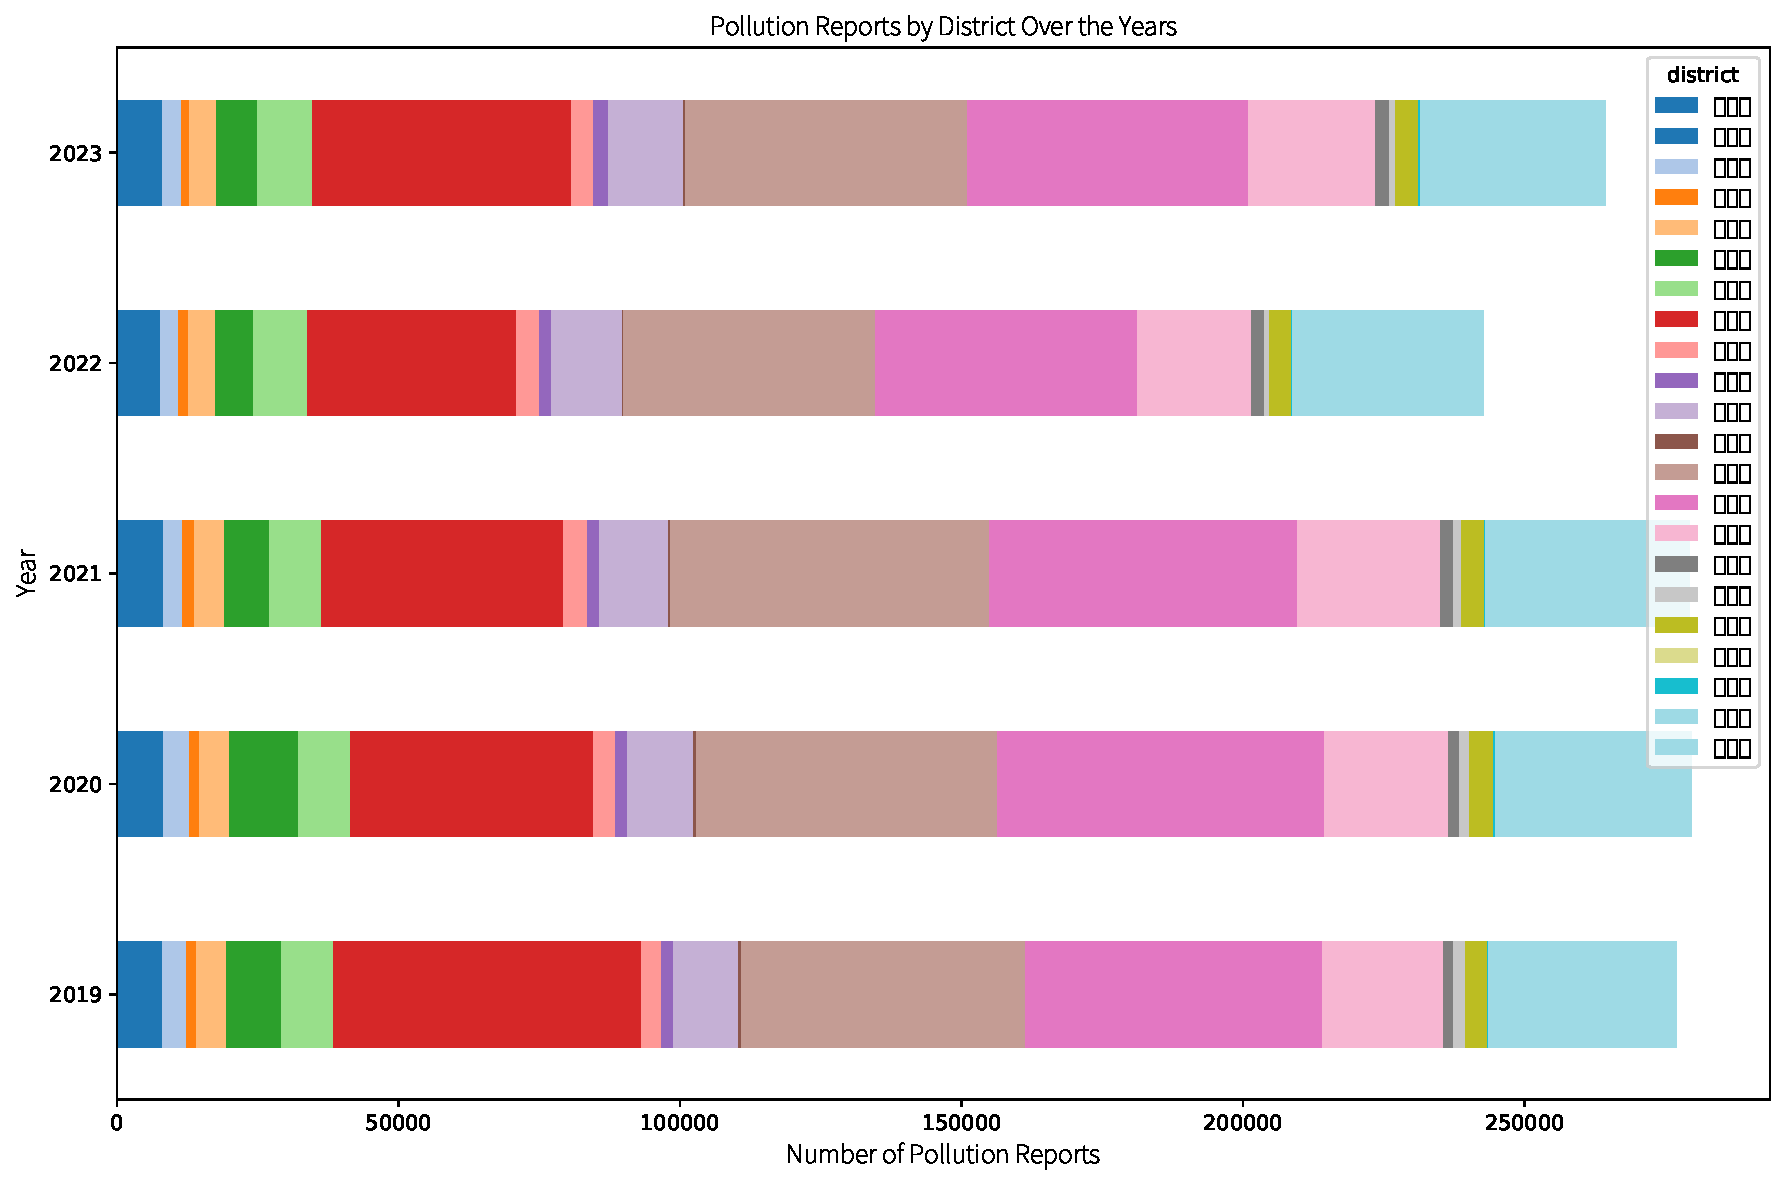
\includegraphics[keepaspectratio]{_thesis_files/figure-pdf/fig-tw-poll-reports-stack-output-2.pdf}}

}

\subcaption[Pollution Reports in Taiwan by
District]{\label{fig-tw-poll-reports-stack-2}}

}

\caption{\label{fig-tw-poll-reports-stack}}

\end{figure}%

Health and sustainability are inextricably linked. ``Human health is
central to all sustainability efforts.'', \emph{``All of these (food,
housing, power, and health care), and the~stress~that the lack of them
generate, play a huge role in our health''} (Sarah Ludwig Rausch \& Neha
Pathak, 2021).

(Abu El Kheir-Mataria \& Chun, 2025) finds warming climate in the MENA
region (Middle East and North Africa) increases cancer risk in women,
mediated through air pollution and other environmental stressors.

Clean air is a proposed as a \emph{human right} (Baroness Jones of
Moulsecoomb \& Caroline Lucas, 2023) yet air pollution is widespread
around the planet, with 99\% of Earth's human population being affected
by bad air quality that does not meet WHO air quality guidelines,
leading to health problems linked to 6.7 million \emph{premature deaths}
every year (World Health Organization, 2022). Air pollution is linked to
cancer incidence. In Taiwan, South Korea, and England, groundbreaking
research by (Lim et al., 2022) analyzed over 400000 individuals
establishes exposure to 2.5μm PM (PM2.5) air pollution as a \emph{cause
for lung cancer.} In (Hannah Devlin, 2022), professor Tony Mok, of the
Chinese University of Hong Kong explains it plainly, which I want to
quote here in verbatim:

\begin{quote}
\emph{``We have known about the link between pollution and lung cancer
for a long time, and we now have a possible explanation for it. As
consumption of fossil fuels goes hand in hand with pollution and carbon
emissions, we have a strong mandate for tackling these issues -- for
both environmental and health reasons.''}
\end{quote}

The main way to combat air pollution is through policy interventions.
(MARIA LUÍS FERNANDES, 2023) the EU has legislation in progress to curb
industrial emissions. If legislation is in place, causing bad air
quality can become bad for business. In China, (Gu et al., 2023) links
air pollution to credit interest rates for business loans; companies
with low environmental awareness and a history of environmental
penalties pay 12 percent higher interest rates. In France, (Bouscasse et
al., 2022) finds strong health and economic benefits across the board
from air pollution reduction.

Likewise to the lack of clean air, lack of access to sufficient clean
water and water pollution are issues in several places around the world;
globally, 4.4 billion people only have access to water that's not safe
for drinking (Soliman, 2024). Even in wealthy countries like the the US,
with increasing situations of water scarcity and drought due to climate
change, issues of water ownership become increasingly dire. (Koch, 2022;
Naishadham, 2023b) describes a fight in the US over water usage rights
in Arizona, where Fondomonte, a subsidiary of a Saudi Arabian company
that grows a water-hungry crop alfalfa, exacerbating the local water
crisis by using large amounts of public water, leading to public outcry
and being sued for ``public nuisance'' for its excessive groundwater
pumping, and finally cessation of its lease and operations on state
land; but still continuing operations on private land (Naishadham,
2023a; {``Saudi Firm That Grows Hay in {California} and {Arizona} to
Lose Farm Leases over Water Issue,''} 2023).

Water quality is highly dependent on competent governance. For example,
in the U.S., the national government recently rolled back rules for
water safety, which had only been implemented last year, to protect the
consumer from per- and polyfluoroalkyl substances (PFAS) (Trager, 2025).
Once pollution is in the environment, cleaning it up is very expensive.
For instance, in France, where storm water washed pollution into the
waterways feeding into the Seine river, making it unsuitable for
swimming, the city of Paris invested 1.4 Billion Euros to create a
massive underground reservoir and a water cleaning system by the opening
of the Paris Olympics in 2024 - and still the water quality would be
variable based on rain incidence (Walt, 2023).

Water and soil pollution are highly connected, as water flows through
soil. In Saudi Arabia, (Picó et al., 2023) used wild and ruderal plants
as bioindicators to detect pollution of air, water and soil,
specifically anthropogenic pollution, pharmaceuticals, pesticides, and
other industrial chemicals, concluding both Abha and Riyadh showed
notable levels of pollutants while Riyadh (a city with more industry)
showed higher levels of pollution.

Improved farming practices directly improve soil structure (reducing
runoff and contamination) and water retention, thereby mitigating both
soil degradation and water pollution. Participants in the 2023 Baltic
Sea Action Group for the EIT Food Regenerative Agriculture project
(which so far has trained over 1200 farmers and 160 farmers advisory
groups in regenerative practices), highlighted practical
soil‐restoration methods in their respective countries: applying
\emph{biochar} on pilot plots in the Czech Republic increased water
retention by up to 20\%, no‐tilling and cover‐cropping practices in
Hungary boosted insect‐species counts by 15 points, and adopting
regenerative crop rotations in Bulgaria cut synthetic fertilizer use by
25\%; one of the challenges remains consumer awareness: only 12\% of
consumers in Central and Eastern Europe currently recognize the
``regenerative'' label - awareness must grow to drive demand (Baltic Sea
Action Group, 2023).

A practical example of the interconnection between water pollution,
agriculture, architecture, and extreme weather, are bioswales, which
help catch storm debris and reduce water pollution. In Taiwan, (劉大正,
2010) showed that grass swales increase infiltration, reduce runoff, and
improve downstream water quality, helping stabilize slopes via enhanced
drainage (Taiwanese landscape is very mountainous, with); in a follow up
field trial at a National Highway in Gangshan, grass swales consistently
trapped sediments and adsorbed heavy metals from highway runoff before
those pollutants could reach nearby waterways.

The above examples from around the world suggest that
\emph{``regenerative''} is not just a buzzword or wishful thinking -
instead, it maps to a set of concrete practices and approaches to
improve the condition of the living environment under threat from
pollution.

\subsubsection{Climate Disaster Preparedness: Extreme Weather
Resilience}\label{climate-disaster-preparedness-extreme-weather-resilience}

The Word Economic Forums Global Risks Report 2024 paints a bleak picture
of the future with expectations of increased turbulence across the board
based on a survey of over 1400 topic experts (World Economic Forum,
n.d.). Global warming specifically increases the risk of disasters and
extreme weather events; the US Global Change Research Program presented
a comprehensive report to the US Congress, which links disaster-risk
directly to global warming; for examples increased wildfires damage
property, endanger life and reduces \emph{air quality,} which in effect
increases health challenges (\emph{Fifth {National Climate Assessment}},
2023). Warming global climate has concrete effects on daily life. Warmer
climate helps viruses and fungi spread (Press, 2023). (Williams \&
Joshi, 2013) higher CO\textsubscript{2}eq concentrations in the air can
cause more turbulence for flights. As extreme temperatures are
increasingly commonplace, with observed changes in heatwaves, there's
increased risk of wildfires (Perkins-Kirkpatrick \& Green, 2023; Volkova
et al., 2021), while flood risk mapping might lower property prices in
at risk areas (Sherren, 2024). Summers of 2022 and 2023 were the hottest
on record so far, with extreme heat waves recorded in places around the
world (Douglas, 2023; Falconer, 2023; National Oceanic and Atmospheric
Administration (NOAA), U.S. Department of Commerce, 2023; NOAA National
Centers for Environmental Information, 2023; Serrano-Notivoli et al.,
2023; Venturelli et al., 2023).

The part of Earth where the \emph{human climate niche} is becoming
smaller (McKibben, 2023). As temperatures rise, certain cities may
become uninhabitable for humans (CBC Radio, 2021). The summer of 2023
saw extensive wildfires in Spain, Canada, and elsewhere; rapidly moving
fires destroyed the whole city of Lāhainā in Hawaii (Anguiano, 2023). In
California, (Jerrett et al., 2022) says, \emph{``{[}w{]}ildfires are the
second most important source of emissions in 2020''} and \emph{``negate
reductions in greenhouse gas emissions from other sectors.''} Some parts
of South America have seen summer heat \emph{in the winter}, with
heatwaves with temperatures as high as 38 degrees (Livingston, 2023).

In Taiwan disaster risk and hazard mapping is well-developed, with early
warning systems, and comprehensive response preparedness - and painful
experiences - instrumental to saving lives (Y.-J. Tsai et al., 2021).
Intensifying storms forming near coastlines, can be expected with
\emph{``{[}c{]}hanges to tropical cyclone trajectories in Southeast Asia
under a warming climate''} (Garner et al., 2024). The situation on the
Pacific and Atlantic oceans is not dissimilar, with
\emph{``{[}o{]}bserved increases in North Atlantic tropical cyclone peak
intensification rates''} (Garner, 2023).

In the Phillipines, with increasing extreme weather events,
\emph{``businesses are more likely to emerge in areas where
infrastructure is resilient to climate hazards''} (Y. Cheng \& Han,
2022). Across several case studies, (Fabris \& Luburić, 2022) discusses
vulnerable sectors from agriculture to transport, under threat from
extreme weather events, such as floods, heatwaves, droughts, and storms
impact human health: societal development and economic growth should be
realistic on planning for weather-related impacts.

Climate-related disasters can spur action as extreme weather becomes
visible to everyone. After large floods in South Korea in July 2023 with
many victims, president Joon promised to begin taking global warming
seriously and steer the country towards climate action (AFP, 2023; Al
Jazeera, 2023; Web, 2023). South Korea has a partnership with the
European Union (European Commission, 2023a).

\subsection{Financialization of Nature vs Sacred Value: Scaling Up
Sustainable
Action}\label{financialization-of-nature-vs-sacred-value-scaling-up-sustainable-action}

There are 2 main approaches to protecting nature:

\def\pandoctableshortcapt{Economics of Nature Commodification vs Sacred
Economics}

\begin{longtable}[]{@{}
  >{\raggedright\arraybackslash}p{(\linewidth - 2\tabcolsep) * \real{0.3611}}
  >{\raggedright\arraybackslash}p{(\linewidth - 2\tabcolsep) * \real{0.6389}}@{}}
\caption[Economics of Nature Commodification vs Sacred
Economics]{Economics of Nature Commodification vs Sacred
Economics}\tabularnewline
\toprule\noalign{}
\endfirsthead
\endhead
\bottomrule\noalign{}
\endlastfoot
\textbf{Economics of Nature Commodification} & \textbf{Economics of the
Sacred} \\
Measure and assign monetary value to nature. & Nature is Sacred - such
as are religious holy places - and can't be touched (Eisenstein, 2011,
2018) \\
\end{longtable}

\let\pandoctableshortcapt\relax

The question of whether we should we put a price on nature (or is it
time to leave utilitarian environmentalism behind?) is still openly
debated, with pro-financialization voices arguing assigning monetary
figures to nature's benefits legible to policymakers and markets,
channeling large sums into conservation (e.g.~carbon/biodiversity
credits), while critics argue monetary metrics flatten relational,
cultural and intrinsic values of ecosystems into exchange-value and
commoditize nature, which may legitimize offsetting schemes that
displace rather than prevent damage (Leverhulme Centre for Nature
Recovery, 2023).

Ecosystem services literature defines a ``Nature's Contributions to
People'' framework, originally proposed by the Intergovernmental
Science-Policy Platform on Biodiversity and Ecosystem Services (IPBES).
(Díaz et al., 2018). (Muradian \& Gómez-Baggethun, 2021) critically
assess the framework, arguing utilitarian and anthropocentric views of
the ecosystem services concept perpetuates problematic dualisms (humans
and nature are separate) - and call for a new approach centered on
ecology.

\def\pandoctableshortcapt{Defining Ecosystem Services Concepts}

\begin{longtable}[]{@{}l@{}}
\caption[Defining Ecosystem Services Concepts]{Defining Ecosystem
Services Concepts from (Leverhulme Centre for Nature Recovery,
2023)}\tabularnewline
\toprule\noalign{}
\endfirsthead
\endhead
\bottomrule\noalign{}
\endlastfoot
9 Steps Towards Defining Ecosystem Services \\
Identify ecosystem functions \\
Quantify ecosystem functions \\
Identify ecosystem services \\
Quantify ecosystem services \\
Quantify financial value of ecosystem services \\
Assign property rights \\
Create ecosystem service markets \\
Commodify nature \\
\end{longtable}

\let\pandoctableshortcapt\relax

A practical example of ecosystem services becoming a common language
comes from (Z. Zhang et al., 2023) who proposes integrating ecosystem
services conservation into urban planning, so biodiversity could become
part of city planning. Another example is tourism, a large industrial
sector which relies on ecosystem services (L. Li et al., 2023). In
Taiwan, (T. H. Lee et al., 2021) developed a framework of indicators to
assess sustainable tourism.

\subsubsection{Ecological Restoration: Damaged Ecosystems, Agroforestry
\&
Permaculture}\label{ecological-restoration-damaged-ecosystems-agroforestry-permaculture}

The concept of how a public resource is over-used until breaking down as
each user only bears a fraction of the cost - know as \emph{tragedy of
the commons} - was described by the ecologist Garrett Hardin in 1968
(Hardin, 1968; Lopez et al., 2022; Meisinger, 2022; Murase \& Baek,
2018). When so many systems are broken, some argue sustainability is not
enough and we should work on \emph{regeneration} of natural habitat. The
UN announced 2021-2030 the Decade on Ecosystem Restoration, which
includes a wide range of regenerative action (Fischer et al., 2021). For
instance, (Han \& Chen, 2022) identifies nature-based solutions ``land
re-naturalization (such as afforestation and wetland restoration)''

\def\pandoctableshortcapt{Regenerative Actions}

\begin{longtable}[]{@{}l@{}}
\caption[Regenerative Actions]{Non-Exhaustive list of Regenerative
Actions from (Han \& Chen, 2022)}\tabularnewline
\toprule\noalign{}
Non-Exhaustive list of Regenerative Actions \\
\midrule\noalign{}
\endfirsthead
\toprule\noalign{}
Non-Exhaustive list of Regenerative Actions \\
\midrule\noalign{}
\endhead
\bottomrule\noalign{}
\endlastfoot
Afforestation \\
Wetland restoration \\
 \\
\end{longtable}

\let\pandoctableshortcapt\relax

The organic food and drink market is growing worldwide, with gross sales
in 2019 totaling over 106 billion euros, albeit being a small percentage
of total food industry (Gamage et al., 2023). Growing organic food poses
many challenges, which farmers need to adapt to, in order to participate
in regenerative food systems. One approach is growing food forests, also
known as agroforestry, which integrates farming into natural
environments, achieving CO\textsubscript{2}eq storage in the soil
through agriculture and forestry using agroecological practices.

In Ireland, (Irwin et al., 2023) studied dairy farmers' willingness to
plant trees to increase vegetation cover on their land, finding that
economic incentives alone are insufficient, and support in the form of
advisory and education is needed. Similarly, in the Brazilian Amazon
rainforest (Yadav et al., 2023) finds the active participation of the
local community in planning permaculture practices, enhances their
acceptance and effectiveness. In Bangladesh, (Ruba \& Talucder, 2023)
found agroforestry plays an active role in achieving the country's
Sustainable Development Goals (SDGs), including zero hunger, climate
action, mitigating climate change impacts through CO\textsubscript{2}eq
sequestration, life on land through biodiversity conservation and
improving soil fertility, yet is hindered by the lack of policy support
and educational level of the farmers. In the Baltic Sea region in
North-Eastern Europe and Central Europe face similar challenges, (Baltic
Sea Action Group, 2023) pointing out farmers' traditional mindset as the
biggest obstacle, describing the paradigm shift from extractive farming
to regenerative agriculture, using techniques such as no-till farming,
which reduces soil erosion and improve soil health by reducing synhetic
imputs; yet, it's not only a single practice that is enough,
regenerative agriculture is a holistic approach and agroecology
education programmes need to be comprehehnsive.

(G. Low et al., 2023) further studies how agroforestry deep integration
into food value chains unlocks opportunities for recognition and rewards
from economic actors in the network, underlining how complex and
knowledge-heavy nature of value-capture, calling for further
standardization of practices to reward sustainability practices and
ecosystem services. The challenge lies in that bioeconomy is not
inherently sustainable and may put biodiversity at risk, depending on
the level of industrialization of agriculture and specific practices,
which require deep knowledge and understanding of natural and artificial
interactions the ecological systems; the authors advocate for a precise
distinction between extractive and regenerative practices in
\emph{``bioeconomy''} (Ollinaho \& Kröger, 2023). Finally, taking Brazil
as and example, (De Queiroz-Stein \& Siegel, 2023) argues for an
integration of competing and conflicting bioeconomy policies, in order
to achieve the goals of a sustainable bioeconomy.

Svalbard Seed Vault is an example of seed conservation to safeguard
biodiversity by storing backup seeds of plants from around the world in
cold storage (Asdal \& Guarino, 2018; Westengen et al., 2013). Since its
opening in 2008, the storage solution provided by the Norwegian
government has stored seeds from from 123 genebanks in 85 countries
around the world ({``Arctic Doomsday Seed Vault Gets More Than 14,000
New Samples,''} 2025; The Norwegian Ministry of Agriculture and Food,
2025). (Vitaletti, 2025) proposes using a blockchain-based lottery
system to storage seeds in local refrigerators, in order to enhance
resilience and ensure survival of seeds, by storing seeds in many
locations.

\subsubsection{Energy: Climatech, Renewables, and Decarbonisation
Pathways}\label{energy-climatech-renewables-and-decarbonisation-pathways}

Globally, 34\% of all emissions come from energy production (US EPA,
2016), making it the key sector to require innovate for reducing carbon
emissions. The International Energy Agency's (IEAs), \emph{``Tracking
Clean Energy Progress''} report on 50 distinct decarbonisation enablers
and finds that only 3 components - solar PV, PV electric vehicles, and
building lighting - are on track with the net zero by 2050 scenario,
while 28 need more effort and 22 are ``not on track'' (IEA, 2023b).

Geopolitical situations can affect technology adoption; after Russia's
war in Ukraine, Europe needed to quickly reduce consuming cheap Russian
fossil fuel energy (in the form of gas) (Bonasia, 2024). In 2024, for
first time in Europe, renewables in the form of wind and solar energy
surged past production of fossil fuels (Beer, 2024; Graham \& Fulghum,
2024). Meanwhile, China is experiencing a solar installation rush before
a deadline set by a new renewable pricing policy; from January to April
2025, a record-breaking 105 gigawatts (GW) of solar capacity was
installed, bringing the total solar power close to 1 TeraWatt, predicted
to make solar power China's main energy source in 2026(Carrie Xiao,
2025; L, 2025a; Redazione, 2025; Weaver, 2023; Y. Zhu, 2023).

(Gaure \& Golombek, 2022) simulate a CO\textsubscript{2} free
electricity generation system in the European Union where \emph{``98\%
of total electricity production is generated by wind power and solar;
the remainder is covered by a backup technology.''}. The authors
stipulate it's possible to power the EU without producing
CO\textsubscript{2} emissions.

EU's energy mix in 2024:

\begin{figure}

\centering{

\pandocbounded{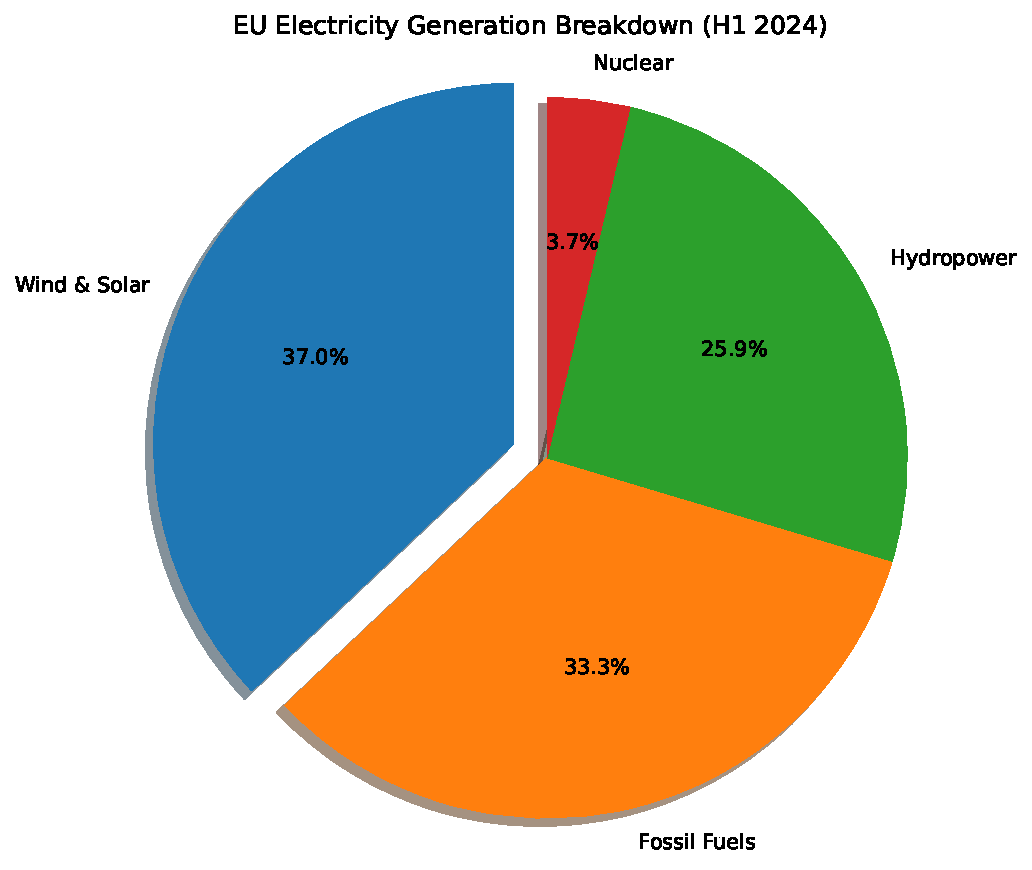
\includegraphics[keepaspectratio]{_thesis_files/figure-pdf/fig-eu-energy-brakdown-output-1.pdf}}

}

\caption[The EU's Energy Production
Breakdown]{\label{fig-eu-energy-brakdown}The EU's Energy Production
Breakdown}

\end{figure}%

Wind and solar energy overtook fossil energy in Europe:

\begin{figure}

\centering{

\pandocbounded{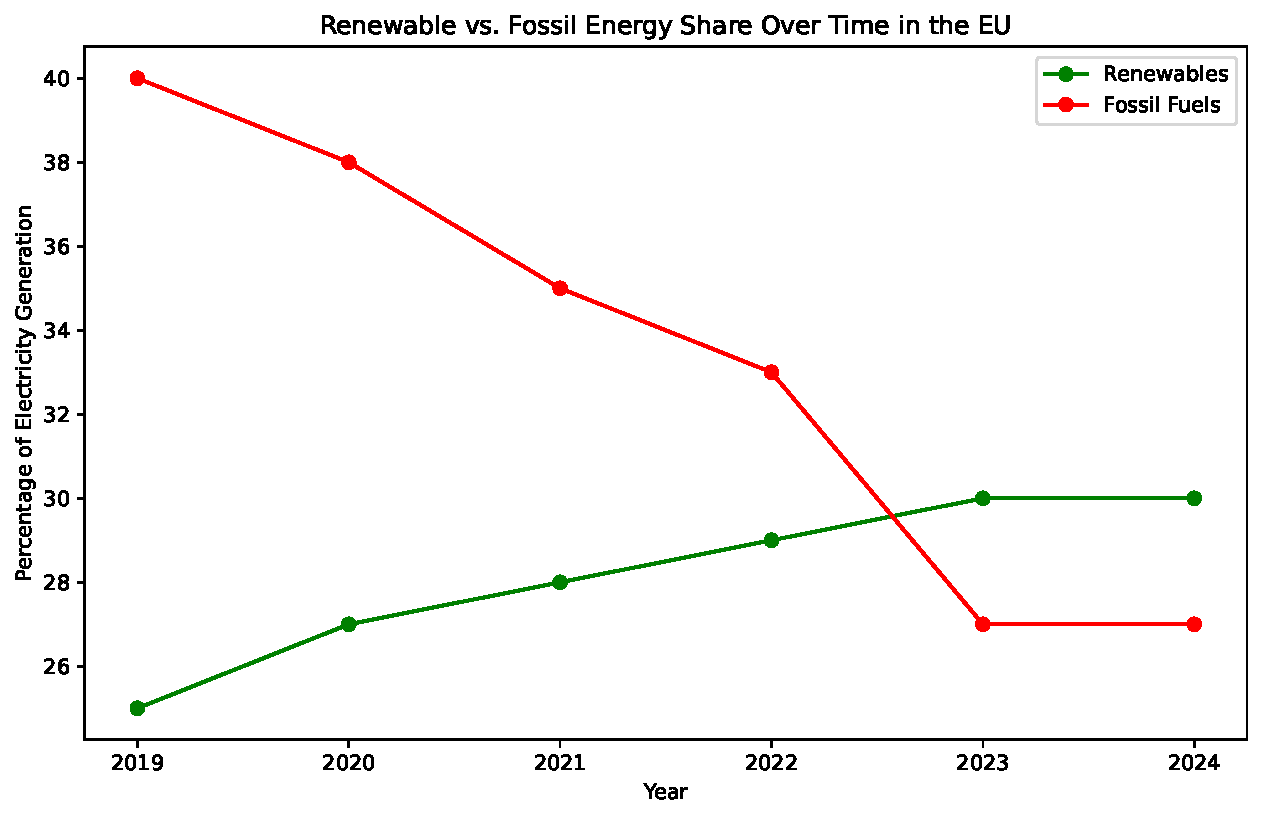
\includegraphics[keepaspectratio]{_thesis_files/figure-pdf/fig-eu-renew-vs-fossil-output-1.pdf}}

}

\caption[The EU's Renewables vs Fossil
Energy]{\label{fig-eu-renew-vs-fossil}The EU's Renewables vs Fossil
Energy}

\end{figure}%

Globally, renewables also overtook fossil fuels (IEA, 2024):

\begin{figure}

\centering{

\pandocbounded{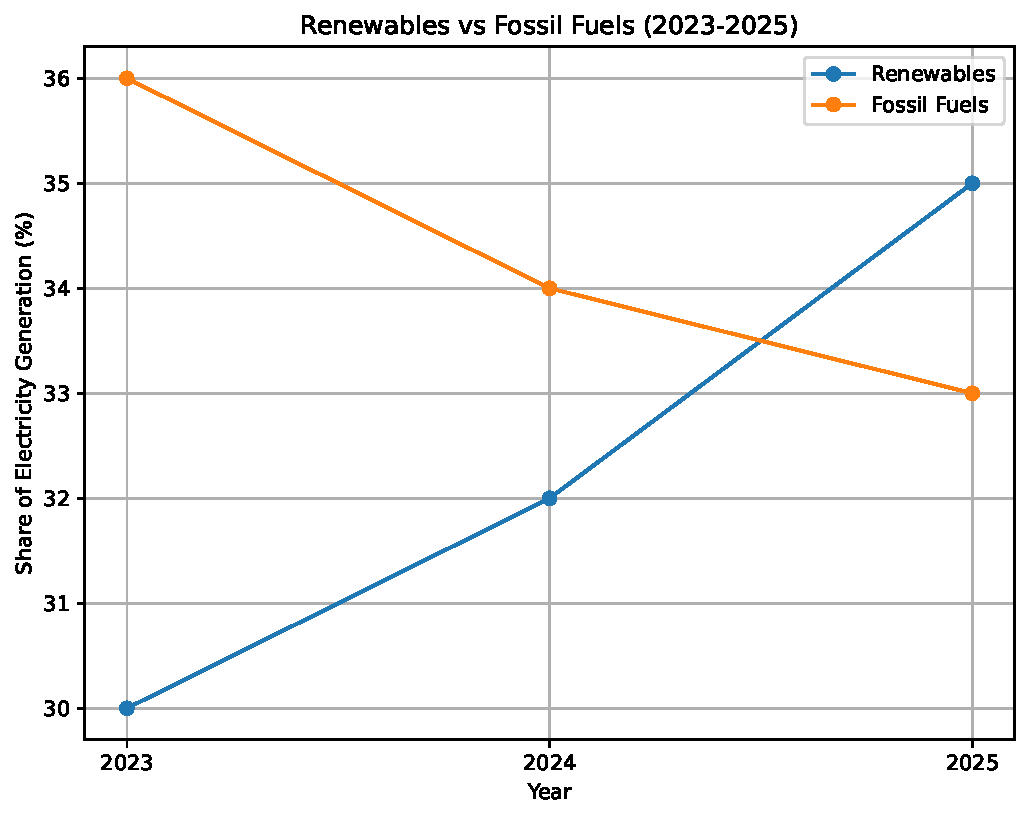
\includegraphics[keepaspectratio]{_thesis_files/figure-pdf/fig-global-renew-vs-fossil-output-1.pdf}}

}

\caption[Global Renewables vs Fossil
Energy]{\label{fig-global-renew-vs-fossil}Global Renewables vs Fossil
Energy}

\end{figure}%

Meanwhile, reduction in coal-power was also possible. Coal is a large
CO\textsubscript{2}eq emitter.

\begin{figure}

\centering{

\pandocbounded{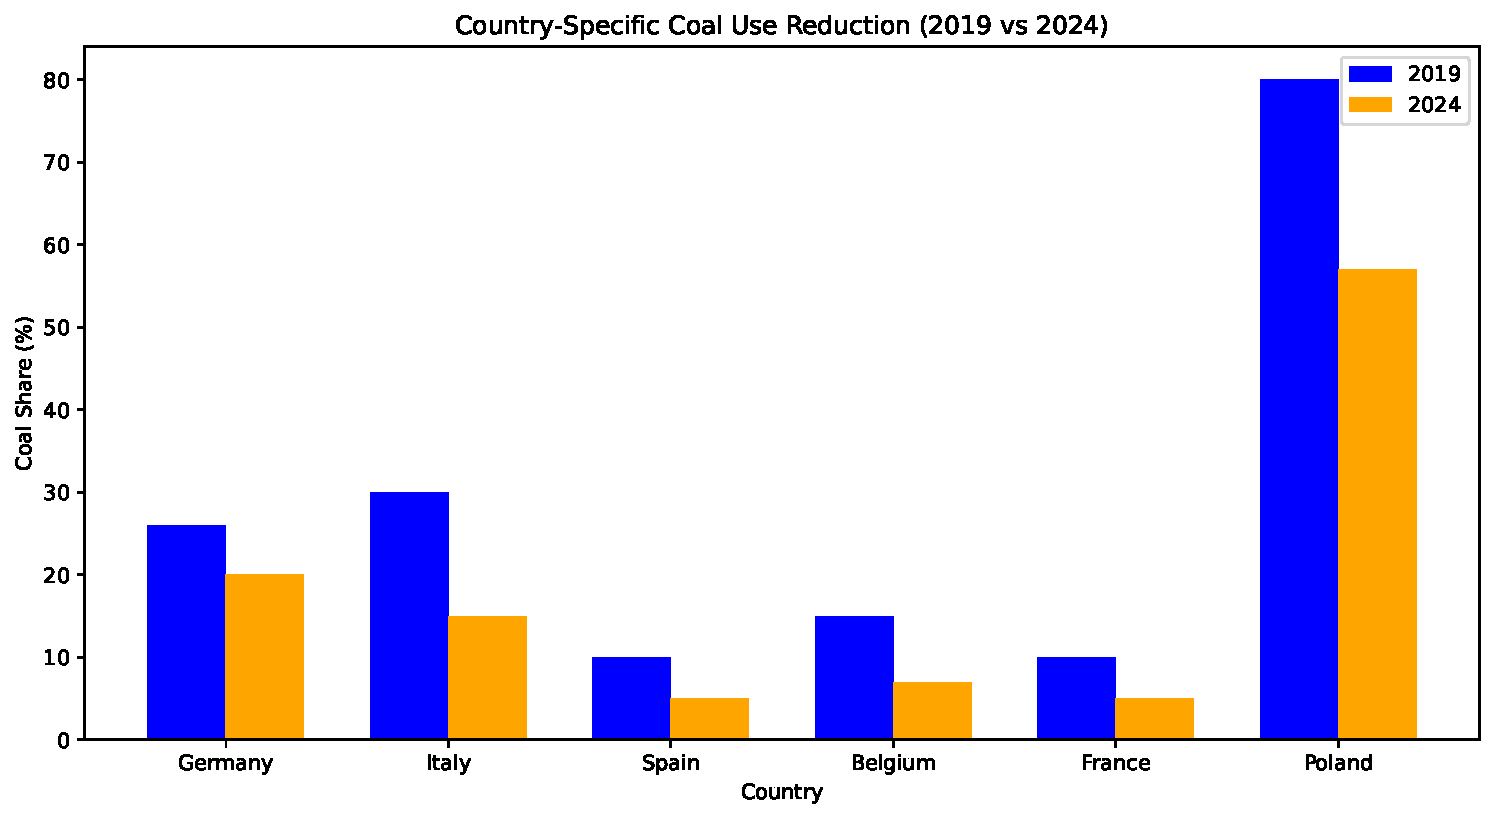
\includegraphics[keepaspectratio]{_thesis_files/figure-pdf/fig-renew-vs-fossil-output-1.pdf}}

}

\caption[The EU's Reduction of Coal
Energy]{\label{fig-renew-vs-fossil}The EU's Reduction of Coal Energy}

\end{figure}%

\begin{figure}

\centering{

\pandocbounded{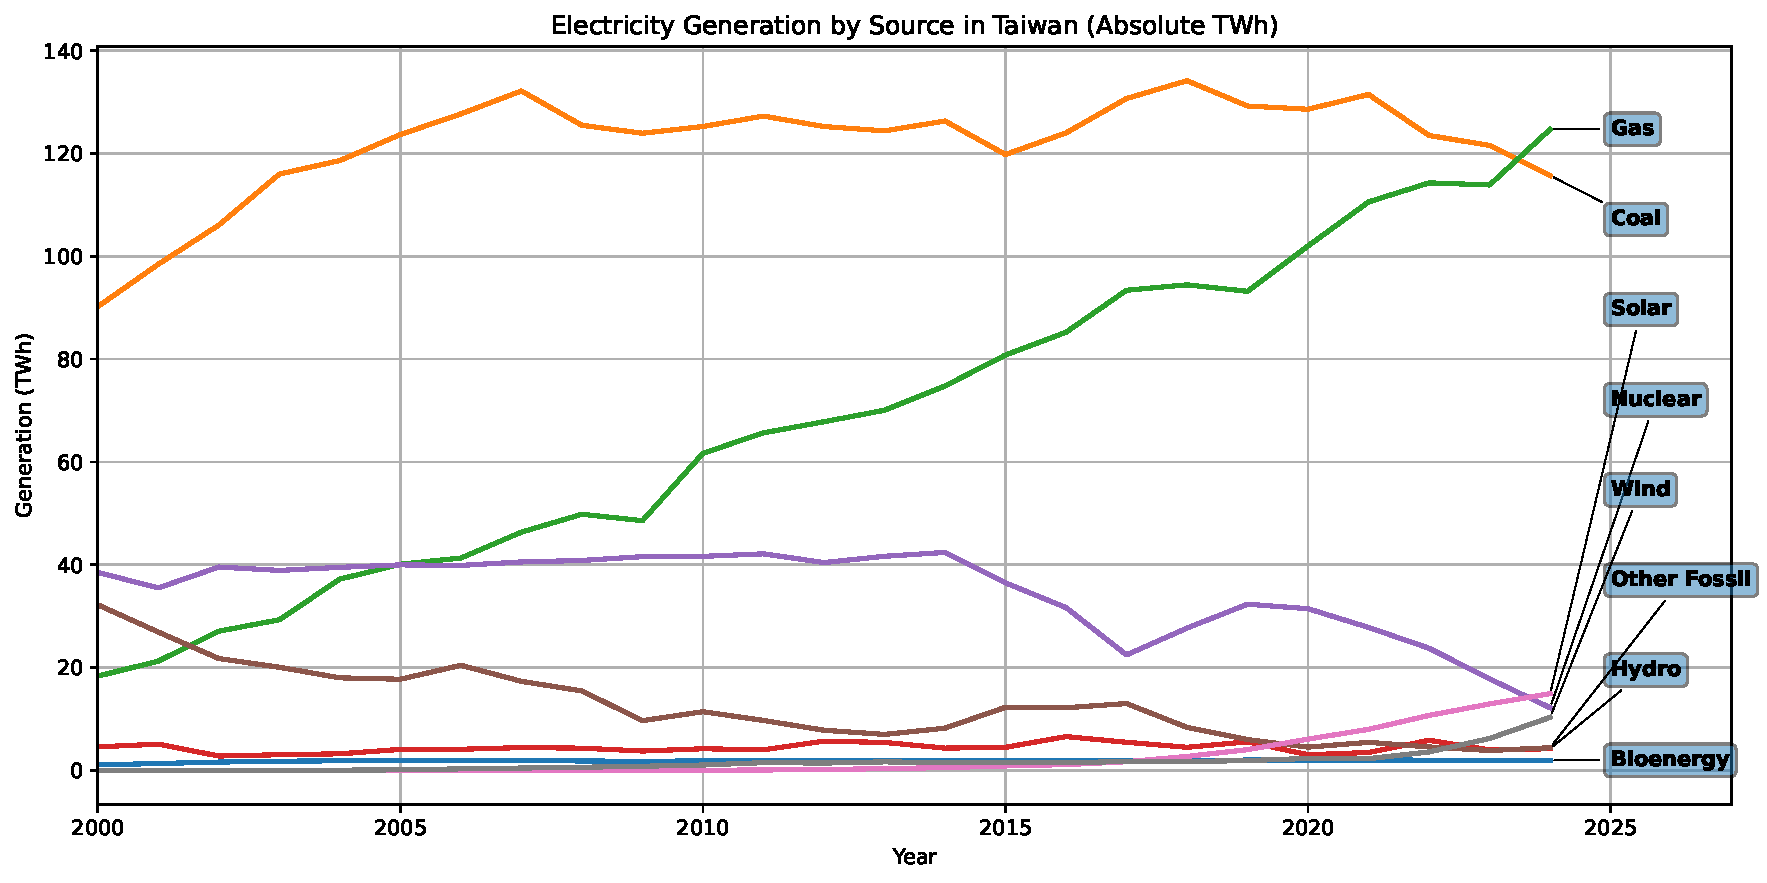
\includegraphics[keepaspectratio]{_thesis_files/figure-pdf/fig-tw-energy-prod-output-1.pdf}}

}

\caption[Taiwanese Energy
Production]{\label{fig-tw-energy-prod}Taiwanese Energy Production}

\end{figure}%

Beyond electricity and heat, the chemical sector is a massive
CO\textsubscript{2}eq source. (Lange, 2021) reports the petrochemical
industry uses about 10\% of global fossil carbon as feedstock and
another 7\% to power its processes, producing some 400Mt of base
chemicals each year, 36\% of which becomes packaging; the cradle-to-gate
CO\textsubscript{2}eq emissions for base chemicals are roughly 1--2.5kg
CO\textsubscript{2}eq per kg or 5t CO\textsubscript{2}eq per tonne of
plastic, when including use and end-of-life, the entire lifecycle
emissions are 1.7Gt CO\textsubscript{2}eq (∼4\% of all anthropogenic
emissions) per year; a true circular-carbon economy would require
renewable carbon feedstocks (e.g.~biomass or CO\textsubscript{2}-derived
monomers), electrified green heat, closed-loop catalytic recycling of
molecular building blocks, and modular low-temperature reactors to slash
energy demand.

Large technology conglomerates and newly founded startups alike are
working in the climate solutions space (often referred to as
\emph{climatech} by the media), have proposed a range of approaches to
CO\textsubscript{2} reduction in the Earth's atmosphere. These
technologies include several types of \emph{carbon capture}, directly
from the air (direct air capture or DAC), from the source of pollution,
such as using high--performance filters on factory chimneys, as well as
nature-based solutions such as large scale tree planting using drones.
Each technology has their own pros and cons. For instance, (Vitillo et
al., 2022) illustrates how direct air capture of CO\textsubscript{2} is
difficult because of low concentration and CO\textsubscript{2} capture
at the source of the emissions is more feasible. (Cleantech Group, 2023)
profiles 100 innovators across agriculture, food, energy, mobility, and
waste that Cleantech Group judges most likely to enable a future with
sub-2 degrees warming. Overall, considering pathways to carbon drawdown
finds considerable uncertainty exists among experts which
CO\textsubscript{2}eq reduction among nature- and technology-based
methods are the most effective (S. Low et al., 2022).

\subsubsection{Individual Action}\label{individual-action}

Sometimes individual environmental (climate) action \emph{does matter}
and can come at great personal cost, even loss of life. EJAtlas tracks
environmental justice cases around the world, where human stakes are
very high Scheidel et al. (2020).

However, for most of us individual climate action is \emph{ineffective}.
The effect of individual climate action such as \emph{choosing a more
sustainable product} is so limited to be next to meaningless. For
individual consumer choices to make a difference, they need to be
\emph{aggregated} into a movement, collective action with scale,
influence, and visibility.

There is no single solution to the environmental crisis. Given the
enormity of environmental degradation, many different approaches are
needed. This chapter documents some of the ongoing work which a
sustainability companion could assist college students get involved
with.

While the scale of climate change is too big for individual action to
make a difference, individual action can foster hope and a sense of
collective responsibility (Nature, 2020).

\newpage

\section{Design}\label{design}

\begin{figure}[H]

{\centering \pandocbounded{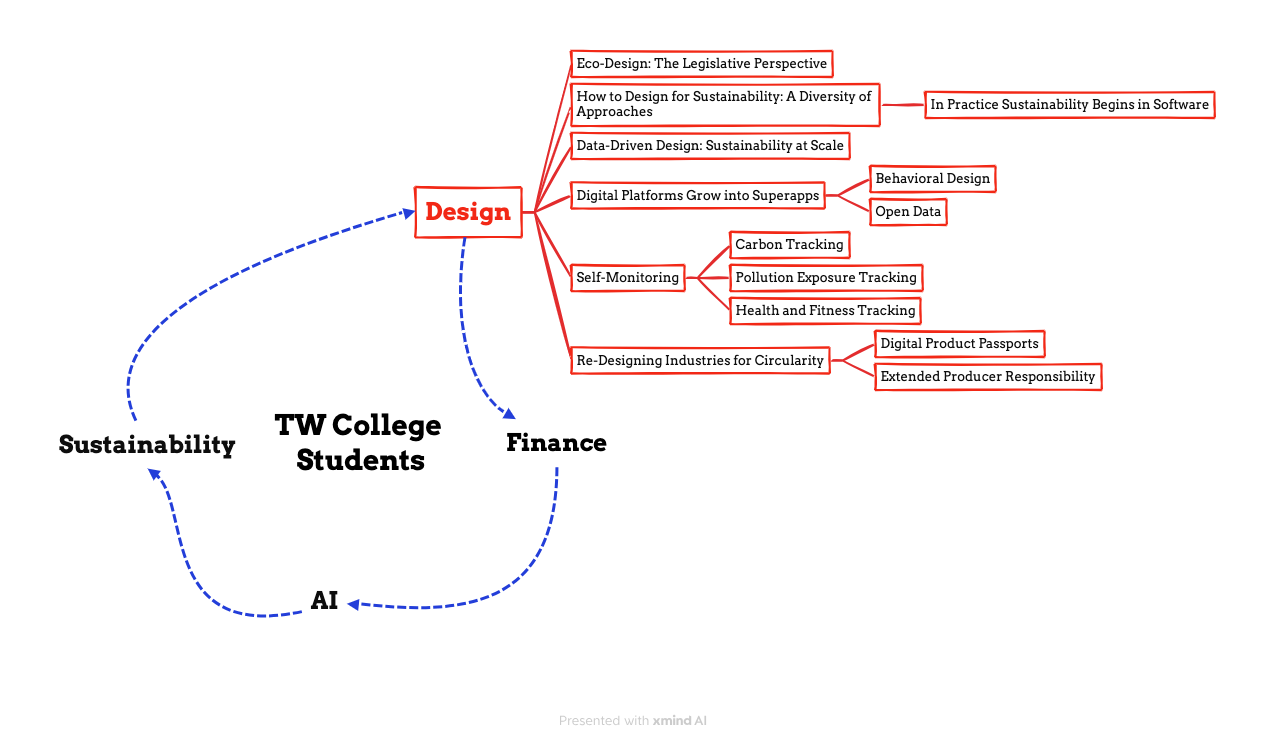
\includegraphics[keepaspectratio]{./images/design/abstract-design.png}}

}

\caption{Visual abstract for the design chapter}

\end{figure}%

Designers have been battling complexity since the beginning of design.
Industrial designer Dieter Rams famously said in the 1970s \emph{``Good
design makes a product understandable''} as one of the ten key tenets to
strive for in good products (DW Euromaxx, 2018; Fabrique \& Q42, n.d.).
Don Norman, the grandfather of interaction design, is quoted as saying:

\begin{quote}
``Modern technology can be complex, but complexity by itself is neither
good nor bad: it is confusion that is bad.'' - (Norman, 2016)
\end{quote}

I would simply say: Design makes complexity comprehensible.

Sustainability is one of the most complex goals that humanity has set
for itself. The following looks at some of the ways design might make
it.. achievable.. and comprehensible.

\subsection{Eco-Design: Design as Political Action at
Scale}\label{eco-design-design-as-political-action-at-scale}

Politics matters in sustainability. In Brazil, deforestation fell 60\%
in 1 year, based on remote satellite reconnaissance, after the election
of a more pro-environment leadership (Watts, 2023). Globally, the
monumental task of removing several gigatons of CO\textsubscript{2e}
from the atmosphere requires massive policy shifts and collaboration
across countries and industries (Mackler et al., 2021).

In Europe, the EU ``Green Deal'' legislative strategy is comprehensive
and backed by science, with the EU Commission having released strategic
foresight reports since 2020, and becoming a driving force of
transformative climate legislation in Europe (European Commission,
2023b). The timeline of the policy context in Europe is as follows: in
2019, the von der Leyen commission adopted the European Union (EU) Green
Deal strategy. In 2021 the Commision proposed a goal of reducing
CO\textsubscript{2}eq emissions by 55\% by 2030 under the \emph{Fit for
55} policy package consisting of a wide range of economic measures. In
November 2022, the proposal was adopted by the EU Council and EU
Parliament with an updated goal of 57\% of CO\textsubscript{2}eq
reductions compared to 1990, set to become a binding law for all EU
member countries (\emph{{EU} Reaches Agreement on National Emission
Reductions}, 2022; European Commission, 2019c, 2019a; European Council,
2022). In March 2022, the EU Circular Economy Action Plan was adopted,
looking to make sustainable products \emph{the norm} in EU and
\emph{empowering consumers} as described in (European Commission,
2022a).

Designing the right legislative measures can be hugely impactful.

Consumer products' overall life-cycle environmental impact is defined in
the design process by the materials and energy resources needed and the
post-consumer potential for reuse or recycling. In the context of the
European Union, \emph{eco-design} has gained political support from
European Commission as part of the EU's \emph{``Green Deal''}
legislative strategy, aiming to transform European economies into
sustainability leaders (Commission et al., 2014). The Ecodesign for
Sustainable Products Regulation (ESPR) entered into force in July 2024
(European Commission, 2024b) following the (European Parliament, 2022)
proposal whereby the European Commission established a general framework
for \emph{eco-design: ``requirements for sustainable products, repealing
rules {[}referring to the previous Eco-Design Directive (2009/125/EC){]}
currently in force which concentrate on energy-related products only,''}
setting up a level playing-field for the organizations operating on the
EU single market. Virginijus Sinkevičius, the EU Commissioner for the
Environment, Oceans and Fisheries, is quoted as describing eco-design as
design that \emph{``respects the boundaries of our planet''} (European
Commission, 2022c).

\def\pandoctableshortcapt{The Qualities of \emph{Eco-Designed Products}}

\begin{longtable}[]{@{}
  >{\raggedright\arraybackslash}p{(\linewidth - 2\tabcolsep) * \real{0.5000}}
  >{\raggedright\arraybackslash}p{(\linewidth - 2\tabcolsep) * \real{0.5000}}@{}}
\caption[The Qualities of *Eco-Designed Products*]{The 9 qualities of
\emph{eco-designed products} based on the Ecodesign for Sustainable
Products Regulation (ESPR) enacted as law in the EU as of July 2024
(European Parliament, 2022; Lüttin, 2025).}\tabularnewline
\toprule\noalign{}
\begin{minipage}[b]{\linewidth}\raggedright
Feature
\end{minipage} & \begin{minipage}[b]{\linewidth}\raggedright
Benefit
\end{minipage} \\
\midrule\noalign{}
\endfirsthead
\toprule\noalign{}
\begin{minipage}[b]{\linewidth}\raggedright
Feature
\end{minipage} & \begin{minipage}[b]{\linewidth}\raggedright
Benefit
\end{minipage} \\
\midrule\noalign{}
\endhead
\bottomrule\noalign{}
\endlastfoot
Durable & Reduces the need to frequently replace the product \\
Reusable & Extends the product's life-cycle; sell or share to the next
user \\
Reparable & Extends the product's life-cycle; fix instead of
discarding \\
Upgradable & Extends the product's life-cycle; improve performance
without complete replacement. \\
Easy to Maintain & Reduce resources needed to keep the product
functional \\
Easy to Refurbish & Support second-hand use and circular economy \\
Easy to Recycle & Support material recovery at end of the product's life
to reduce new resource extraction and pollution \\
Energy Efficient & Reduce product's CO\textsubscript{2}eq footprint and
operating costs \\
Resource Efficient & Reduce product's use of raw materials and energy
during production and life-cycle \\
\end{longtable}

\let\pandoctableshortcapt\relax

Eco-Design for Sustainable Products is a key EU sustainable policy
design tool and each product covered by the ESPR is required to have a
\emph{Digital Product Passport} (DPP) which enables improved processing
within the supply chain and includes detailed information to empower
consumers to understand the environmental footprint of their purchases
(European Commission, 2022b). It's safe to say the large majority of
products available today do not meet these criteria. Given this
far-reaching legislative effort, we have an opportunity to re-imagine
how every product can be an eco-product and how they circulate in our
circular economy. The Director of the French environmental NGO Pôle
Eco-conception describes eco-design as ``{[}l{]}ocated at the interface
between consumption and production patterns, eco-design helps to
structure the market for products and services using a life cycle
approach and tangible criteria'' (Chouai \& Mayer, 2024).

The European Commission is set to propose a legally-binding 90\%
emissions reduction from 1990 levels to be achieved by 2040; however,
political pushback by governments is likely to weaken the goal; the EU
climate chief Teresa Ribera is looking for ways to find pragmatic
solutions, by, for example, considering some use of carbon credits (thus
far, all the goals needed to be achieved within the borders of EU;
buying carbon credits from places outside the EU would not be counted as
emissions reduction) (Taylor, 2025; Weise, 2025).

\begin{figure}[H]

{\centering 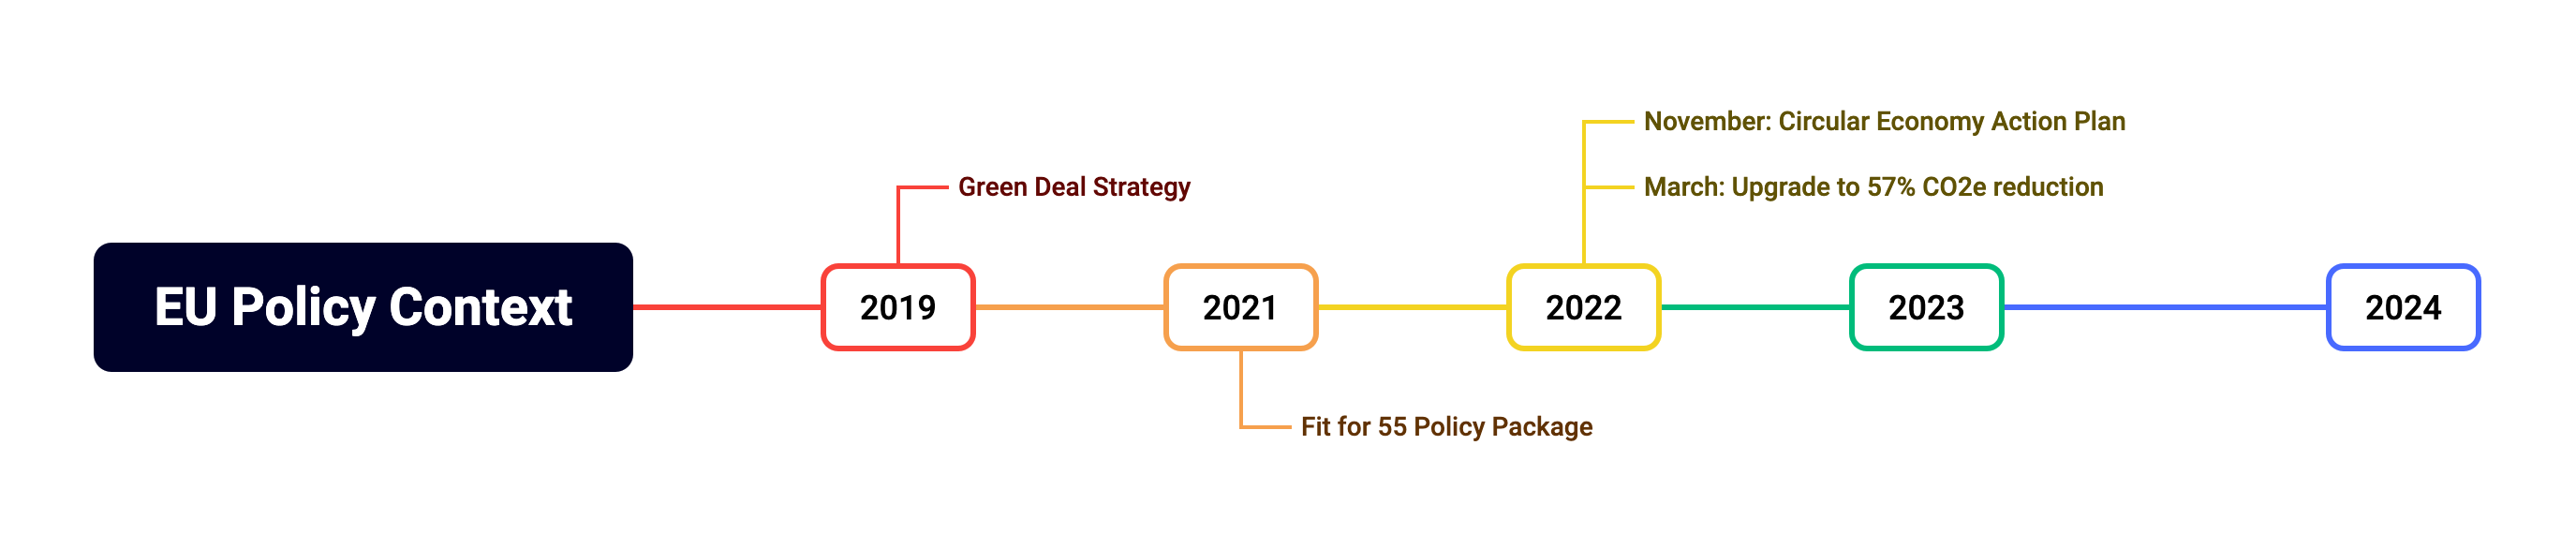
\includegraphics[width=1\linewidth,height=\textheight,keepaspectratio]{./images/sustainability/eu-policy-context.png}

}

\caption{EU Policy Context Timeline}

\end{figure}%

The above chart shows how the European Union has been on a path of
climate legislation transformation.

\begin{figure}

\centering{

\pandocbounded{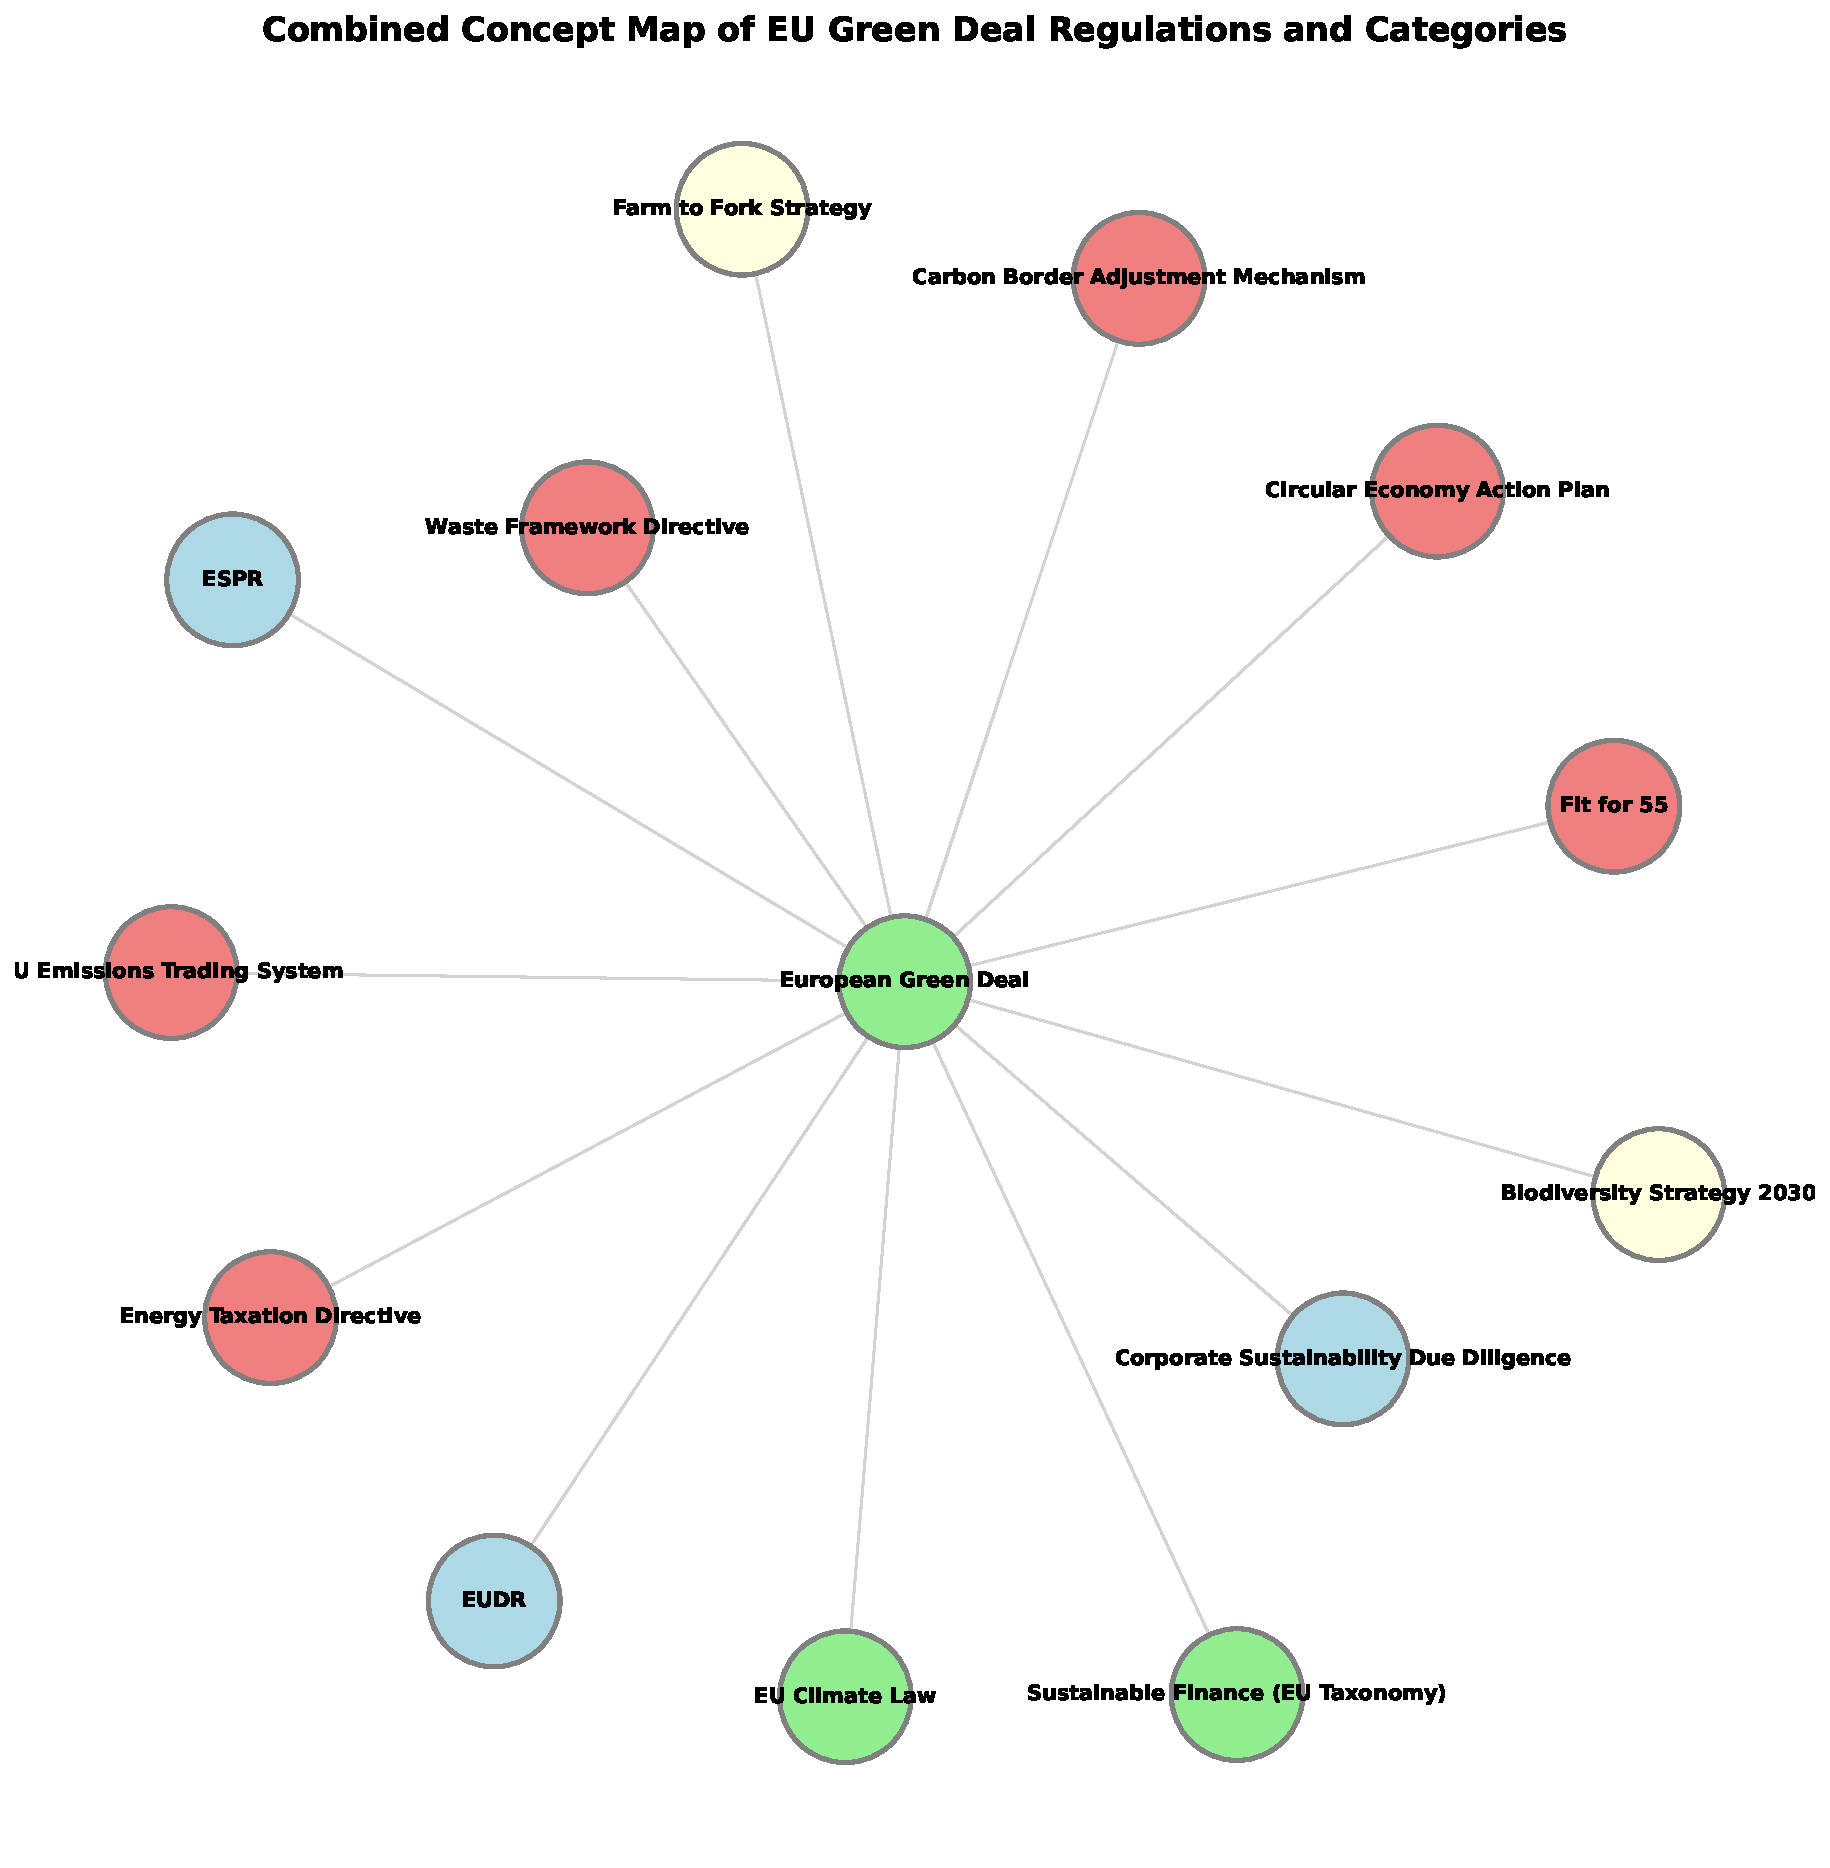
\includegraphics[keepaspectratio]{_thesis_files/figure-pdf/fig-eu-green-deal-output-1.pdf}}

}

\caption[The EU's Green Deal]{\label{fig-eu-green-deal}The EU's Green
Deal}

\end{figure}%

The above chart illustrates the European ``Green Deal''.

In the countries that make up the European Union (EU), a wide range of
legislative proposals, targets, organizations, and goals have existed
for decades. It's not that the EU didn't have an overarching
environmental policy before; rather it was vague and filled with
loop-holes. Upcoming laws cited above aim to harmonize approaches to
sustainability and raise standards for all members states, in turn
influencing producers who wish to sell in the EU common market. National
governments need to adapt EU legislation to local contexts. For example
Estonian government adopted the Estonian Green Deal Action Plan (Eesti
Rohepöörde Tegevusplaan) (Eesti Vabariigi Valitsus, 2022). From the
legislative perspective, NFRD (Non-Financial Reporting Directive) is
replaced by CSRD (Corporate Sustainability Reporting Directive) and ESRS
reporting is the standard to meet CSRD requirements.

The EU is also concerned with supply-chain deforestation. The ESPR
(Sustainable Products) and EUDR (European Union Deforestation
Regulation) work hand-in-hand as part of EU's legislative efforts to
promote sustainability. EUDR applies to all products placed on the
market from December 2024 and June 2025 for small businesses. Greenpeace
has called the EUDR \emph{``first step to end its complicity in the
reckless destruction of these life-support systems''} - yet to become a
success story, there needs to be follow through, integrating forest
protection throughout the economy. Some of the steps to achiveve this
include the EU \emph{taxonomy of environmentally sustainable economic
activities} published by the Technical Expert Group (TEG) on sustainable
finance, as detailed in the report by (\emph{{EU} Taxonomy for
Sustainable Activities}, n.d.). The proposal for a Nature Restoration
Law by the European Commission requiring member countries to restore
20\% of EU's degraded ecosystems by 2030 and full restoration by 2050
has not yet passed (as of writing) (\emph{Scientists Urge {European
Parliament} to Vote for Nature Restoration Law}, 2023) and is facing a
backlash (David Pinto, 2023).

Certainly the EU is not the only region legislating to promote
sustainability; sustainability policy context is shifting around the
world. There are legislative efforts in numerous jurisdictions, which
have passed laws which aim to reduce the environmental impact of
products throughout their lifecycles. In the US, the \emph{Inflation
Reduction Act} provided funding to development of de-carbonizing
technologies and includes plans to combat air pollution, reduce green
house gases and address environmental injustices (Rajagopalan \&
Landrigan, 2023). In Australia, the Product Stewardship (PS) scheme also
includes an investment fund targeted at increasing the recycling rates
of specific products (Australian Government, 2024). Australia, Japan,
and Taiwan all have sustainable procurement schemes, prioritizing
greener products in public purchases (Australian Government Department
of Finance, 2025; Ministry of the Environment, Government of Japan,
2000; The Ministry of Environment of Taiwan, 2024).

I was torn whether to place \emph{politics} under \emph{sustainability}
or \emph{design}, and decided for the latter - as sustainability is
primarily \emph{descriptive}, using science to measure and present the
real situation, while design is \emph{prescriptive}: codifying decisions
about how do we live - in products and services. Design \emph{is}
political.

\subsubsection{Beyond Recycling: Default to Return, Repair,
Reuse}\label{beyond-recycling-default-to-return-repair-reuse}

(Gigerenzer, 2008) argues that heuristics - basically, rules of thumb -
can make more accurate predictions about the future than statistical
tools such as Bayesian and regression models, in certain contexts,
especially when data is incomplete or noisy. This aligns with Herbert
Simon's classic concept of bounded rationality, which suggests that
people make decisions not by fully optimizing, but by satisficing,
i.e.~seeking good-enough options given limited time, information, and
cognitive capacity (Simon, 1955). (Gigerenzer, 2008; Gigerenzer \&
Selten, 2002) updated the concept to introduce the idea of a toolbox of
fast, dynamic, frugal heuristics - named ecological rationality, showing
how humans use only a small amount of information, often ignoring most
available data, adapting to specific environments: heuristics aren't
irrational; they work well because they exploit the structure of
real-world environments.

In the practice of design for sustainability, the recognizing that
humans use heuristics, translates to making strategic use of choice
architecture and \emph{the power of defaults}: displaying the most
sustainable option as the default - the oft-quoted example being green
power as the default choice on the German energy markets (Antonides \&
Welvaarts, 2020; Kaiser et al., 2020). Several research projects of
plant-based, vegan and vegetarian food defaults at (university) canteens
show 45-58\% increase in sustainable choices across studies (Boronowsky
et al., 2022; Erhard et al., 2023; Ginn \& Sparkman, 2024; A. W. Zhang
et al., 2024). (Simon Sterne, 2023) argues good UX is about helping the
user make decisions, which can be thought of as four key tactics: (1)
simplify complex choices, (2) intelligent defaults, (3) clear real-time
feedback on the outcome of each option, and (4) avoid unintended regret
by testing decions support aid systems.

The universal recycling symbol creator Gary Anderson created the symbol
when he was an architecture student at USC (University of Southern
California) in 1970 at the age of 23, inspired by Silent Spring, Earth
Day, the Bauhaus, Bucky Fuller, Spaceship Earth, printing presses, and
the Woolmark logo for wool industry certification, and even the Mobius
strip, for a competition held by a packaging firm that was making paper
containers for packaging (Swap Society, 2023).

\subsubsection{Eco-Modulation: Extended Producer Responsibility
Incentive
Design}\label{eco-modulation-extended-producer-responsibility-incentive-design}

Eco-modulation is a legislative innovation, which makes harder to
recycle items more expensive for the producer. Recycling fees take into
account eco-design: an item from a single material is easier (cheaper)
to recycle than product from composite materials. Eco-modulation makes
the hidden cost of hard-to-recycle formats directly visible on the
invoice.

While Taiwan doesn't yet have a specific eco-design law, there are
various pieces of legislation promoting circular economy. Already in
1988, Taiwan implemented an Extended Producer Responsibility (EPR)
scheme, followed by a recycling system (initially focused on electronic
items) in 1998 (Chong et al., 2009). Eco-design initiatives in Taiwan
started at least as early as 1994, when Taiwanese companies and
universities noticed international sustainability trends and began to
implement their own sustainable design initiatives (Jahau Lewis Chen et
al., 2005).

The key to comparing Product Stewardship, Extended Producer
Responsibility (EPR), and Eco-Design is the scope, as illustrated in the
chart below. While Product Stewardship (PS) and Extended Producer
Responsibility (EPR) deal mostly with the end of the product life-cycle
(they are \emph{reactive}), including their disposal and recycling (EPR
going a step further than PS by shifting the responsibility to the
producer), eco-design moves sustainability up the design chain (being
\emph{pro-active}), setting standards for making better products - in
essence, attempting to \emph{design-out} the waste.

\begin{figure}

\centering{

\pandocbounded{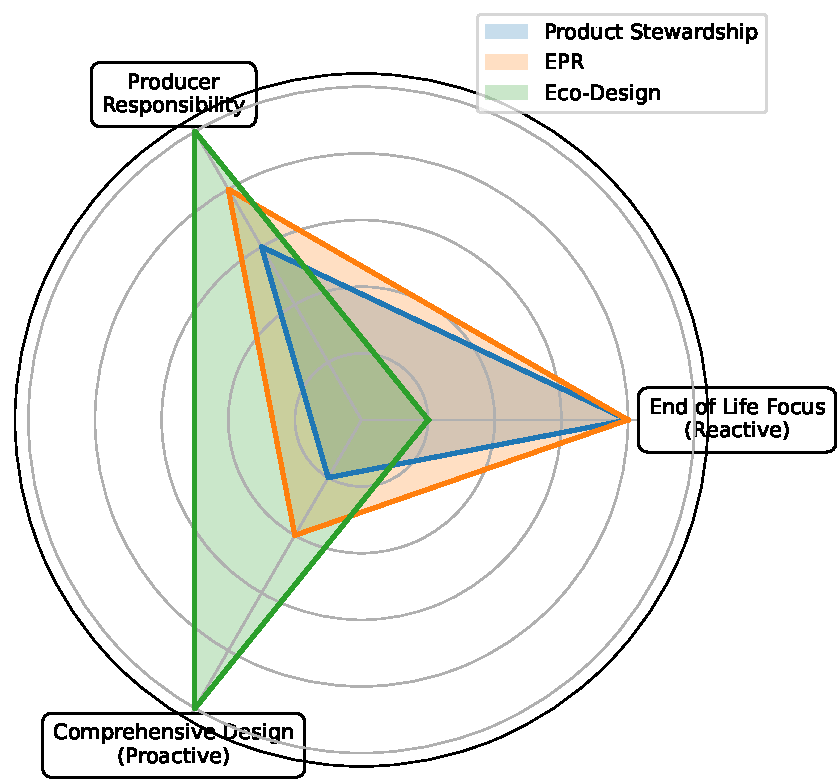
\includegraphics[keepaspectratio]{_thesis_files/figure-pdf/fig-ps-epr-output-1.pdf}}

}

\caption[Extended Producer Responsibility vs Product Stewardship vs
Eco-Design]{\label{fig-ps-epr}Extended Producer Responsibility vs
Product Stewardship vs Eco-Design}

\end{figure}%

Popular blogs such as (Kohli, 2019) and (Lose, 2023) offer many
suggestions how designers can help people become more sustainable in
their daily lives yet focusing on the end-user neglects the producers'
responsibility - termed Extended Producer Responsibility or ERP in waste
management studies.

Extended Producer Responsibility (EPR) is a policy tool first proposed
by Thomas Lindhqvist in Sweden in 1990 and described in detail in his
PhD thesis (Lindhqvist, 2000; Lindhqvist \& Lidgren, 1990), aimed to
encourage producers take responsibility for the entire life-cycle of
their products, thus leading to more eco-friendly products. In essence,
Extended Producer Responsibility enables companies to be resposible for
the entire life-cycle of the product. In California, part of the EPR
regulation is a large pool of funding for cleaning up historic pollution
resulting from industry Moolman (2024).

Nonetheless, EPR schemes do not guarantee circularity and may instead be
designed around fees to finance waste management in linear economy
models (Christiansen et al., 2021). The French EPR scheme was upgraded
in 2020 to become more circular (Jacques Vernier, 2021). In July 2024,
Latvia was the 4th EU country to join an textile-EPR scheme ({``New
{EPR} Requirements for Textiles in {Latvia} from {July} 2024 On,''}
2024). Strong consumer protection legislation (such as EPR) has a direct
influence on producers' actions. For example, in (HKTDC Research, 2022),
the Hong Kong Trade Development Council notified textile producers in
July 2022 reminding factories to produce to French standards in order to
be able enter the EU market.

In Europe, there's large variance between member states when in comes to
textile recycling: while Estonia and France are the only EU countries
where separate collection of textiles is required by law, in Estonia
100\% of the textiles were burned in an incinerator (as of 2018) while
in France textiles are covered by an Extended Producer Responsibility
(EPR) scheme leading to higher recovery and recycling rates (European
Commission. Joint Research Centre., 2021; Nordic Council of Ministers,
2020). Yet, some countries like Germany (75\%), Netherlands (45 \%), and
Denmark (43\%), which have no specific EPR scheme for textiles, report
higher collection rates than France, which with EPR collected only 38\%
of the textiles, however recovered 95\% of that through reuse and
recycling (Eurostat, 2022; \emph{Towards 2025 - Separate Collection and
Treatment of Textiles in Six {EU} Countries}, 2020).

The success of EPR can vary per type of product. For car tires, the EPR
scheme in the Netherlands claims a 100\% recovery rate
(Campbell-Johnston et al., 2020). (J. Peng et al., 2023) finds that the
\emph{Carbon Disclosure Project} has been a crucial tool to empower
Chinese auto-producers to adopt ERP schemes. Technological advancements
play a big role in recycling rates, as even badly sorted materials can
increasingly be recovered using AI; one example being Greyparrot AI,
which notes that even in the most advanced countries, 40\% of waste
sorting is still manual, opening an opportunity for automation (Natasha
Lomas, 2024).

While recycling rates are improving, (Steenmans \& Ulfbeck, 2023) argues
for the need to engage companies through legislation and shift from
waste-centered laws to \emph{product design regulations}. In the same
vein, and in the spirit of EU's EPR regulations, (Ruiz-Pastor \& Mesa,
2023) proposes an integrated \emph{product repairability index} (PRI).
(Lenovo, 08-29-22) suggests rethinking product design entirely to
inspire consumers expect more from the devices they buy. (Duriez et al.,
2022) shows how simply by reducing material weight of the product, it's
possible to design more sustainable transportation. However, the devil
is often in the details. (Formentini \& Ramanujan, 2023) study of Design
for Circular Disassembly (DfCD), introduces a Disassembly Effort Index
(DEI) to measure the disassembly time in seconds; their case study of
the End-of-Life (EoL) of an electrical kettle showed ignoring realistic
EoL failures (such as rusted screws), can lead to inaccurate
recommendations for circular design parameters.

Packaging is a rapidly growing industry, expanding on the back of online
shopping, which generates large amounts of waste materials, which if not
reused or recycled, easily becomes garbage. Over 161 million tonnes of
plastic packaging is produced every year (Bradley \& Corsini, 2023).
Already more than a decade ago, ({``Detail-Rich Sustainable Packaging
{Product Database} Is an Industry First,''} 2010)proposed a database of
green packaging to compare hundreds of sustainable packaging materials
and guide designers through environmental, performance, and cost
trade-offs in one unified tool, in order to help producers choose better
packaging - yet the problem is far from solved. More recently, (Bradley
\& Corsini, 2023) developed an analytical framework of key
sustainability factors, from an overview of 107 studies on reusable
packaging, finding customer acceptance, high return rates, supply-chain
shortening, and system standardization, as the key factors critical to
unlocking reusable packaging solutions at scale. A survey by PMMI, the
Association for Packaging and Processing Technologies, among industry
professional, found legacy equipment, higher material costs, and supply
consistency as the top barriers to sustainable packaging; in turn, vital
enablers were clear vendor guidance, proven material and equipment
solutions, and customer demand ({``Challenges and {Opportunities} in
{Sustainable Packaging Today},''} 2022). In response to legacy equipment
issues, ({``Sulapac -- {Replacing} Plastic,''} n.d.) a large producer of
packaging, has proposed a wood-based, microplastic-free composites to
serve as drop-in replacements for plastics; a material even compatible
with existing molding, extrusion, and thermoforming production lines,
while slashing cradle-to-gate CO\textsubscript{2} emissions and
preventing microplastic pollution.

In food packaging specifically, (Ada et al., 2023) identified distinct
challenges from consumer acceptance to material-supply mismatches,
collection logistics, and regulatory gaps, underscoring the multifaceted
barriers to circular food packaging. Over 85\% of companies in the
``protein industry'': meat, poultry, seafood, and alternative proteins
have some type of sustainability initiative ({``Protein {Brands} and
{Consumers Alike Focus} on {Sustainability},''} 2022). Yet, having
sustainability programs does not make a company sustainable, case in
point being Coca Cola in the beverage industry. (Lerner, 2019) describes
Coca Cola's plastic pollution problem, based on leaked audio, detailing
how Coca-Cola was exposed for lobbying against container-deposit laws -
aka Deposit Return Schemes (DRS), - aiming to misrepresented recycling
as a complete solution; strategies that stalled effective legislation
and maintained a ``green'' facade despite obstructing real
sustainability progress.

The \emph{``Plastic Waste Makers Index''} report lists large
corporations which produce plastic waste globally and provides some
useful statistics: single-use plastic rose by 6 million tonnes from 2019
to 2021, while just 3 million tonnes of recycling capacity was planned
by 2027 (as of the report date, 2023); in total, single-use plastic
generated 450 million tonnes of CO\textsubscript{2}eq emissions per
year; up to 98\% of the single-use plastic was produced from virgin
petrochemicals, while 2\% was from recycled material; meanwhile in
Taiwan, the Far Eastern New Century company boosted recycled content
from 2\% to 11\% per cent in 2021 and plans to double its recycling
capacity (Minderoo Foundation, 2023). (Yap et al., 2023) Singapore
disposes of 900,000 tonnes of plastic waste each year, out of which only
4\% is recycled. Single-use plastics make up 44-68\% of all waste mapped
by citizen scientists (Kiessling et al., 2023).

\subsubsection{Scenario-Building: The Worst Futures and Designs for
Quality of
Life}\label{scenario-building-the-worst-futures-and-designs-for-quality-of-life}

Scenario-building is a key tool for sustainability, because
sustainability is so complex. Sustainable design cannot always predict
certain outcomes - instead, it can make use of scenarios to prepare for
several possibilities. In sustainability, there are rarely good choices.
Rather it's a question of avoiding the worst choices. One existing tool,
which has been widely used, is the En-ROADS climate change solutions
simulator; governments, organizations and individuals around the world
have used it explore climate scenarios based on interactive changes and
visualizations (Climate Interactive, n.d., 2023; Creutzig \& Kapmeier,
2020; Czaika \& Selin, 2017). Likewise, (Rooney-Varga et al., 2019)
shows the effectiveness of \emph{The Climate Action Simulation} in
educating users about \emph{success scenarios}. \emph{Life Cycle
Assessment} and \emph{Environmental Impact Analysis} are another set of
useful tools to provide eco-design scenarios (de Otazu et al., 2022).

While traditional economic thinking is based on a conflict between
nature and development, some new holistic models find there is potential
for synergy between economic, social, political, cultural, and
environmental metrics. For example, (Kaklauskas et al., 2023)`s
multi-criteria analysis of 169 countries and 238 cities, finds 71\%
average correlation between Climate Change and Country Success (C3S) and
Quality of Life (C3QL) indicators. In a similar vein, (Rieger et al.,
2023) develops an integrated science of wellbeing, linking humans'
psychological, biological, societal and environmental domains to guide
research and public policy, based on interactions between domain
experts.

Wellbeing Economy Governments is an example of country-level
collaboration in sharing expertise on sustainable development, looking
to bring post growth strategies and policy frameworks to the mainstream.
The concept of a wellbeing economy focuses on human and ecological
wellbeing rather than material growth since 2018 and includes Finland,
Iceland, New Zealand, Scotland, Wales, and Canada as founding members of
the network (Fioramonti et al., 2022).

(Popkova et al., 2022) argues that SDGs need to discussed in their
totality and uses factor analysis to link SDGs to institutions and
digital technologies; findings include SDG 3 (Good Health and
Well-Being) and SDG 17 (Partnerships for the Goals) progress through
institutions in developed countries and are most impacted by digital
technologies and digital knowledge index, meanwhile SDG 16 (Peace,
Justice and Strong Institutions) makes the most headway in developing
countries, which are starting from a lower base. Likewise, the German
Institute of Development and Sustainability (IDOS) has built a tool to
connect SDGs and their 169 targets to NDCs (Nationally Determined
Contributions), looking for synergies for effective climate action plans
and sustainable development strategies, visualizing a clear skew which
SDGs receive the most climate‐related commitments - SDG 2 (Zero Hunger),
SDG 6 (Clean Water and Sanitation), SDG 7 (Affordable and Clean Energy);
meanwhile SDG 14 (Life Below Water), and the SDG 3 social goals
discussed above, SDG 4 (Quality Education) and SDG 5 (Gender Equality),
are the least addressed in climate plans (Dzebo et al., 2023).

Eco-Design is about improving processes and optimizing resources. While
the goal of reducing harm is shared, the specifics will depend on the
industry. (Van Doorsselaer, 2022) Defines eco-design as \emph{``design
for X''} in a circular economy, thinking through the life cycle of a
product, tools, materials, production, use, and end-of-life phases.

In wine-making, (Manzardo et al., 2021) presents an Italian winery case
study, where a redesigned Merlot red wine procedure reduced in
environmental impacts from fuel and pesticide use in vineyards; the
8-step procedure included calculating the product's environmental
footprint and following the ISO 14006 standard, titled
\emph{``Environmental management systems --- Guidelines for
incorporating ecodesign''}. Finding uses for by-products, can improve
sustainability even more. (Iñarra et al., 2022) designed a circular
scheme for brewery left-overs, producing feed ingredients for
aquaculture; in a further step, using life-cycle assessment (LCA) and
optimizing logistics, reduced the aquafeed's environmental footprint
also by 6\%.

In architecture and the built environment, (Munaro et al., 2022)
conducted a comprehensive reviews of eco-design 288 articles,
identifying \emph{Design for Adaptability} and \emph{Disassembly} as the
most inclusive strategies, coining a new term DfAD; a framework linking
DfAD with lifecycle assessment tools is a promising are for research to
support sustainable construction.

In pharmaceuticals, (Bassani et al., 2022) proposes an approach to
eco-design using life-cycle assessment: optimizing packaging types,
alternative materials, transport, and weight reduction. A follow-up
study from the same group in 2023 extended the eco-design to a full
cradle-to-grave assessment and evaluated end-of-life alternatives
(Bassani et al., 2024).

In the printing industry, (Miyoshi et al., 2022) takes the example of
ink toner bottles and applies Life Cycle Simulation to show in a case
study how standardized compatibility between older and newer systems can
save resources and results in sustainability savings, highlighting how
re-manufacturing is an important strategy in circularity for reducing
CO\textsubscript{2} emissions and life cycle costs.

While these examples underline the industry-specificity of eco-design,
some authors attempt to come up with mores holistic approaches. For
instance (Ruiz-Pastor et al., 2022) developed ``CN\_Con'', a metric for
conceptual design, trying to measure circularity and novelty in
conjunction, by analyzing product functions, durability, material
origins, and end-of-life, while at the same time supporting creative and
circular design solutions in early stages.

On an international level, looking at companies operating on the
European Single Market, (Arranz et al., 2022) conducted a large-scale
study using machine learning on firm survey data from 870 organizations
across diverse economic sectors, acquired from the 2015 EU Public
Consultation on the Circular Economy conducted by European Commission,
comparing coercive pressures (regulations, subsidies, grants), normative
pressures (industry standards, professional networks), and mimetic
pressures (competitive imitation), finding normative and mimetic
pressure only enhance sustainability, if coercive pressure already
exists - i.e.~regulations are a key point of leverage. In summary,
enacting laws which support sustainability can shift complex systems
with many parties towards a circular economy, and be enhanced by
additional voluntary forces. However, a comparative analysis of OECD
green growth indicators for the periods 2004--2005 and 2019 across EU
member states found that green transformation do not correlate directly
with development level - instead each country's unique socio-economic
context plays a role: governance quality and income distribution shape
the effectiveness of regulatory frameworks, suggesting that coercive
policies must be tailored to national circumstances in order to
reinforce circular-economy adoption at scale(Cheba et al., 2022).

\subsection{Thinking in Systems to Re-Design Industries or Provenance
and
Traceability}\label{thinking-in-systems-to-re-design-industries-or-provenance-and-traceability}

As of 2025, \emph{circular economy} is a tiny part of the world economy.
(Circle Economy, 2022) reported in 2022 only 8.6\% of world economy was
circular and \emph{100B tonnes of virgin materials} was sourced every
year. An early pioneering innovator, (Jackson, 1996) showed through
detailed case studies how \emph{preventive environmental management},
redesigning industrial production at the source can avert pollution,
laying the conceptual groundwork for today's circular-economy models.
Many companies are investing into transforming their processes.
\emph{``{[}T{]}ransition to a low carbon economy presents challenges and
potential economic benefits that are comparable to those of previous
industrial revolutions''} (Pearson \& Foxon, 2012).

Futurists and visionaries adept at naming things have already listed the
5th, 6th, and even the 7th industrial revolution, pointing at robotics,
quantum computing, nanotechnology, and more, looking at current trends
and building scenarios for 2050 to envisioning a world with convergence
of bio-based and mineral-based technologies, widespread sustainability,
and energy-abundance (Chourasia et al., 2022; Ruiz Estrada, 2024). If
indeed, we're in an industrial revolution, it's possible to re-design
entire industries, and that is exactly the expectation sustainability
sets on businesses. Across all industries, there's a call for more
transparency. Conversations about sustainability are too general and one
needs to look at the specific sustainability metrics at specific
industries to be able to design for meaningful interaction. There's
plentiful domain-specific research showing how varied industries can
develop eco-designed products.

I use the lens of \emph{sustainability} - a complex term - to look at
how design can contribute to eco-friendly products, advocating a diverse
set design methods as a toolbox, where one can pick a suitable tool to
match the problem. While AI allows us to look at a larger number of
design scenarios than previously feasible, there are many approaches to
design for sustainability, with varied design practices that may be
relevant at different times in the process. Designing for sustainability
is fundamentally a hopeful act, imbibed with the belief that a healthier
world is possible - because health and sustainability are intrinsically
connected. As this research is \emph{practice-oriented} (i.e., my goal
here is to find design approaches that could influence my prototype), I
will focus on some fields of design which I hope relevant, fruitful, or
contextual to my project.

\emph{Eco-Design}, \emph{Circular Design}, \emph{Design for Circularity,
Cradle-to-Cradle Design}, \emph{Green Design}, \emph{Regenerative
Design}, \emph{Climate-Responsive Design}, \emph{Life-Centered Design,
Design for Human Rights, Multispecies Design, Designing for Health} -
designing for sustainability has been called with many names in diverse
contexts of use, using a diversity of approaches, with subtle
differences of emphasis and nuance, with same general goal of being more
sustainable. While EU legislation chose \emph{Eco-Design} as the
overarching title, researchers and practitioners discuss all of the
above on a frequent basis. (Ceschin \& Gaziulusoy, 2016) gives a
comprehensive overview of the main themes of sustainable design and the
main contributions and limitations in the well--researched
\emph{``Evolution of design for sustainability: From product design to
design for system innovations and transitions''}.

\begin{figure}

\centering{

\pandocbounded{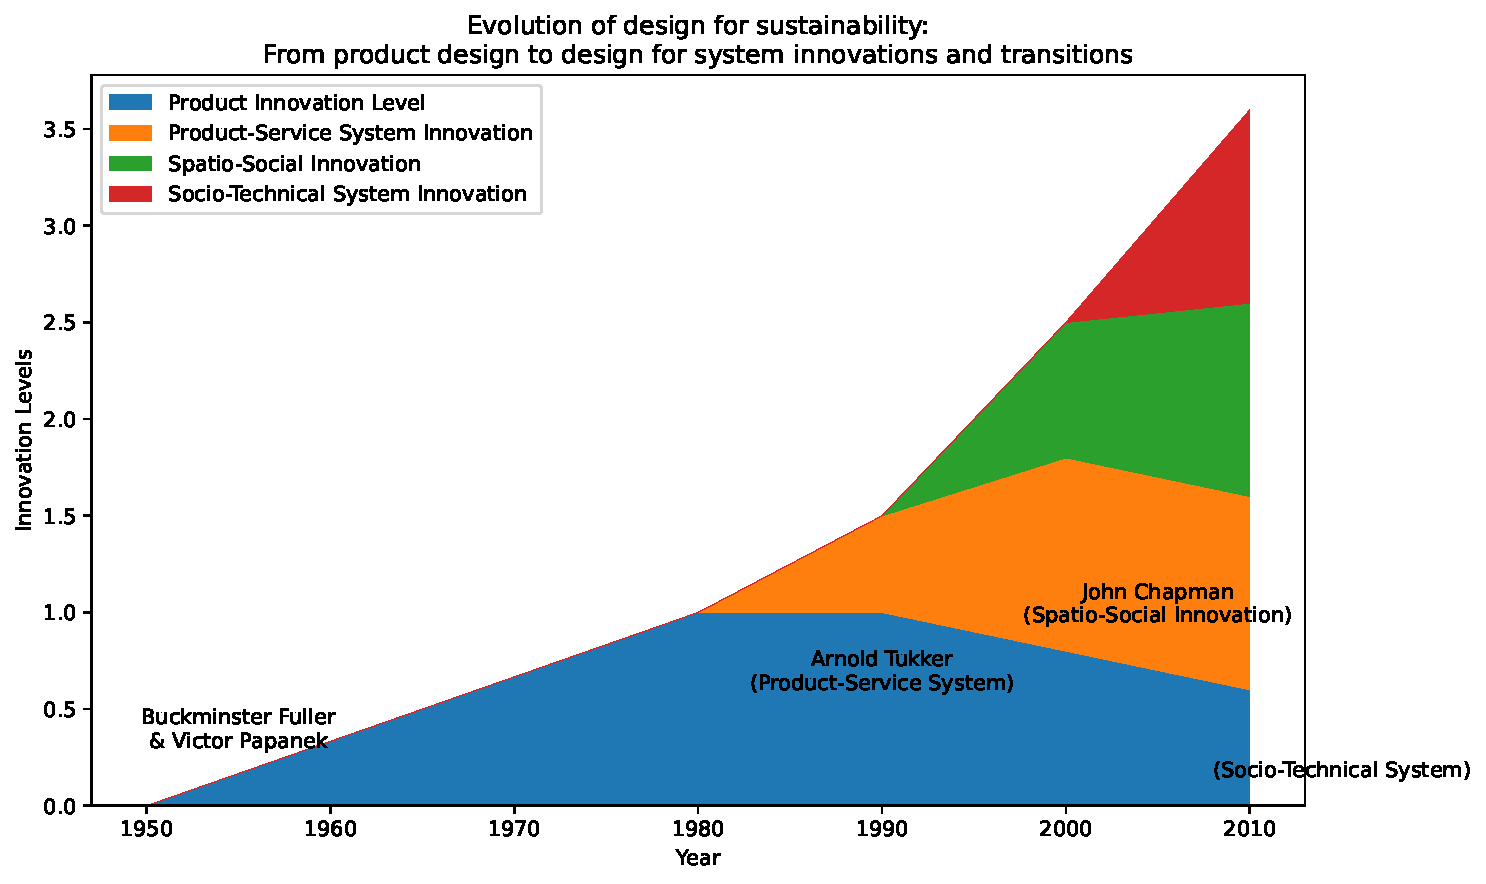
\includegraphics[keepaspectratio]{_thesis_files/figure-pdf/fig-dfs-history-output-1.pdf}}

}

\caption[History of Design for
Sustainability]{\label{fig-dfs-history}History of Design for
Sustainability}

\end{figure}%

\emph{Human-Centered Design} is the grandfather of design with
\emph{attitude}. There's even an ISO standard for human-centered design,
with the designated code ISO9241-210, revised as ISO 9241-210:2019
titled \emph{``Ergonomics of human-system interaction''} and up for
revision soon (ISO standards are reviewed every 5 years). Some of the
key takeaways include ``Understanding and specifying the context of
use'', ``Involving users throughout design and development'',
``Specifying user requirements'', ``Evaluating designs'',
``Multi-disciplinary Collaboration'', ``Iterative process'' and
``Continual Improvement'', and finally - usability is not enough, the
design should provide a user experience (UX) for human ``emotional
responses and satisfaction'' (ISO, 2019).

While \emph{Human-Centered Design} focuses exactly on what it says -
humans - \emph{Life-Centered Design} recognizes human impact on our
surrounding environment as well - making sure we include non-human
animals among our stakeholders. This is where we are getting on the
\emph{territory} of sustainability. While \emph{Human-Centered Design}
is ever popular, the effect humans are having on biodiversity is rarely
considered when designing. \emph{``{[}T{]}he design phase of a physical
product accounts for 80\% of its environmental impact''} notes(Borthwick
et al., 2022) in their framework for life-centered design. If we're
including \emph{other} lifeforms among our stakeholders, what can we
learn from them? \emph{Biomimicry} is about being inspired by nature
while \emph{Biodesign} focuses on design involving biology in the design
itself. Janine Benyus, who coined the word \emph{Biomimicry} (Benyus,
2009) looks at very practical cases of innovation where engineers and
biologist meet and (Dicks, 2023) provides a much more philosophical
account of following the example of nature. Focusing on the financial
sector, (Thomas \& Mantri, 2022)'s philosophical account advocates for
an ``inside-out'' design pattern, much like natural systems, starting
from the smallest structures to guarantee resilience and survival,
instead of trying to control their external environment. In a similar
vein, \emph{Material Ecology} is the wording preferred by the architect
Neri Oxman based at the MIT Media Lab working with biomaterials as a
proponent of \emph{Nature-Centric Design} that adheres to the principles
of ecological sustainability with both an ecologically conscious mindset
and practical toolset (Hencz, 2022). Language and our mental concepts
shape our reality, which makes language-creation an important tool for
sustainability. Neri Oxman's expressions in her (World Economic Forum,
2016) interview introduce some new vocabulary:
\emph{``ecology-indifferent''}, \emph{``naturing''}, \emph{``mother
naturing''}, \emph{``design is a practice of letting go of all that is
unnecessary''}, \emph{``nature should be our single client''}, which
reminds me how self-invented language gives un child-like freedom to
imagine new worlds.

\emph{Regenerative Design} suggests \emph{de}materializing (digitizing)
economies is not enough to be sustainable (by reduction of physical
impact). Design should look beyond reducing harm and find avenues to
\emph{regenerate} damaged or even completely destroyed natural systems
-- ecosystems, biodiversity, land, forests, lakes, rivers - natural
habitats.

\emph{Multi-Species Design} refers to the idea of considering non-human
life-forms as stakeholders of our design. (D. Metcalfe, 2015)`s PhD
Disseration titled \emph{``The devastating effects that unsustainable
design practices have on the natural world and other species with whom
we share this planet''} gives a good overview of the work done is this
branch of design. In a similar vein, \emph{Biodiversity Inclusive Design
(BID)}, developed by (Hernandez-Santin et al., 2023) through a
systematic review of 14 design frameworks, presents a
\emph{'participatory ladder for non-humans'}; including core design
principles that position species' needs within urban planning to achieve
a biodiversity-positive multi-species environment. Multi-species design
and participatory design can work together. (Haldrup et al., 2022)
examines how participatory design can include non-human species as
co-creators of the urban commons; drawing on cases from Copenhagen,
Denmark and the Viskan River (in the textile town, Borås, Sweden), the
authors highlight sensory and aesthetic encounters, and attempts to
perceive the agency of non-human species in a collaborative design
processes (The University of Melbourne, Australia \& Roudavski, 2020).
Multi-Species Design has also entered the art-world thanks to (Marcus,
06-11-23) who uses artworks to think about how material design
strategies, surface textures, substrates, and bio-inspired composites,
can foster biodiversity and interspecies cohabitation in the built
environment. A very practical example helps one visualize this field the
best. (Kosová et al., 2023) introduces the BioGeo Ecotile, a
eco-engineering tile combining pits, holes, grooves, and crevices to
mimic natural rocky shores and provide multi-species
living-environments; deployed on rock armor and flood walls along
Edinburgh's coast in Scotland, Ecotiles supported significantly higher
intertidal species richness compared to smooth tiles, helping animals
make a life there. (Selvan et al., 2023) goes deep into data modeling
multi-variate calculations on how to build buildings, which support
ecology, coming up with a general framework for the architecture of
building envelopes, that resulted in 20\% higher local species richness
and up to 77\% higher abundance for individual species.

In most cases, designing for sustainability makes use of \emph{systems
thinking}, underlining the importance of looking at the entire
life-cycle of a product or service. (Rossi et al., 2022) shows how
introducing sustainability early in the design process and providing
scenarios where sustainability is a metric, it's possible to achieve
more eco-friendly designs. Yet, calculating what's sustainable is hugely
complex because decisions may have unforeseen ramifications. To take a
single example (Nuez et al., 2022) shows how electric vehicles may
increase CO\textsubscript{2} emissions in some areas, such as Canary
Islands, where electricity production is polluting. In sum, sustainable
design encompasses all human activities, making this pursuit an
over-arching challenge across all industries and all human activities
with the complex interdependence contained within these interactions.
(Engkvist, 2024) calls for \emph{Design Sociology}, design should take
account the product's effect on society, giving the example of highly
individualized understanding of individualized psychology and dopamine
cycles for creating social media, while disregarding the societal
effects, such as spread of misinformation. Lack of sustainability in the
design process is a \emph{bug} in the design approach.

\emph{Service Design}, (Ceschin \& Gaziulusoy, 2016) shows how design
for sustainability has expanded from a product focus to systems-thinking
focus placing the product inside a societal context of use. For example
(\emph{Cargo Bike {\textbar} {FREITAG}}, n.d.), recycled clothing maker
FREITAG offers sustainability-focused services such as cargo bikes so
you can transport your purchases and a network for \emph{shopping
without payment} = swapping your items with other members, as well as
repairs of their products. Loaning terminology from \emph{service
design}, the user journey within an app needs to consider each
touchpoint on the way to a state of success. \emph{Designing for Trust},
Weinschenk (2011) says \emph{``People expect most online interactions to
follow the same social rules as person-to-person interactions. It's a
shortcut that your brain uses to quickly evaluate trustworthiness.''}

\emph{Speculative Design} can also help us imagine
\emph{non-anthropocentric} (Edwards \& Pettersen, 2023; Hupkes \&
Hedman, 2022) as well as \emph{dystopian} futures (Pinto et al., 2021).
First introduced by (Dunne \& Raby, 2013) in their seminal book, the
field aims to question the intersection of \emph{user experience design}
and \emph{speculative fiction}. (Barendregt \& Vaage, 2021) explores the
potential of speculative design to stimulate public engagement; thought
experiments can spur public debate on an issue chosen by the designer.
Phil Balagtas, founder of The Design Futures Initiative at McKinsey,
discusses the value of building future scenarios at his talk at Google.
His favorite example, the Apple Knowledge Navigator, first appeared in
an Apple vision video in 1987 and took two decades to materialize in the
real world. It was inspired by a similar device first shown in a 1970s
episode of Star Trek as a \emph{magic device} (a term from participatory
design), which then inspired subsequent consumer product development. It
took another two decades, until the launch of the iPhone in 2007 - a
total of 40 years. Iteration has been the mainstay of software design,
incrementally improving the user experience, through a continuous
feedback loop; yet speculative design can help explore and imagine
possible futures by manifesting them in stories, artifacts, and
scenarios, empowering stakeholders to prepare for challenges and shape
policy, as well as ethical frameworks, beyond strictly product-centered
thinking (Google Design, 2019).

\emph{Participatory Design} and \emph{Speculative Design} can be
complementary as in the work of (Neuhoff et al., 2023), used together to
focus on engaging users deep in the design process to truly understand
their needs, contexts and interactions on a non-superficial level. For
both speculative and participatory design, the cost and makes it into a
niche activity. Generative AI holds the promise to allow designers to
dream up and prototype quicker. In order to build a future, it's
relevant to imagine and critique a future. By being quickly generate
prototypes, once can test out ideas with the future users involving more
of the community and stakeholders. To be able to build something, one
first needs to imagine it; imagination is crucial for change.
Speculative Design helps us envision future scenarios and be critical of
the current reality, by taking an alternative view-point. A related
field, \emph{Design Fiction}, goes even further by creating narratives
and artifacts that immerse participants in detailed visions of possible
futures, blending storytelling and tangible experiences. The
Massachusetts Institute of Technology (MIT) is a source of many
fantastic innovations, used to host The Design Fiction group (from
September 2013 to May 2018), which designed projects to
\emph{``stimulate discussion about the social, cultural, and ethical
implications of emerging technologies''}, coming up with design such as
a Brain-Controlled Interface for Spermatozoa, the Human Perfume,
capturing the smell of the people significant to the author, as well as
Pop Roach, for designing edible cockroaches (Design Fiction group, 2018;
A. Liu, 2017).

\emph{Climate-Responsive Design} embeds a building within the
environmental constraints of a place and looks for opportunities use the
land, wind, sun, local materials, and local vernacular history and
culture when considering a design. Architect Susanne Brorson suggests
sustainability should be considered in the earlier phases of design
instead of trying to fix problems later, discussing
\emph{climate-responsive design principles} (EVM maaarhitektuuri keskus,
2019). The sentiment is echoed by (S. Lee \& Doevendans, 2011) who
edited a volume on sustainable approaches of world-renowned architects:
\emph{``The principles of sustainable design are rooted in the
building's relationship to the site and its environmental conditions
such as topography, vegetation, and climate.''} The pioneering book
\emph{Architecture of the Well-Tempered Environment} laid out ideas for
integrating environmental concerns as part of architecture already in
1980s (Banham, 1999).

\emph{Cradle-to-Cradle Design} uses systems thinking focusing on the
reuse, re-manufacturing, and finally - recyclability - of products. The
Taiwanese Design Research Institute (TDRI) hosted a Nordic Circular
Design Forum in Taipei, where Scandinavian circular design practicioners
shared projects from several industries, highlighting how design
requires building relationships; it's not feasible to create a
sustainable product by oneself, as it takes a whole ecosystem (TDRI,
2021; {``台灣設計研究院({TDRI} ) on {Instagram},''} 2021).
\emph{Durability} is an important dimension for sustainability. High
quality durable products are more sustainable as they last longer and
less likely to be thrown away. Forming an emotional bond with the
product makes it feel more valuable (Zonneveld \& Biggemann, 2014).
(Chapman, 2009) argues in his seminal paper (and later in his book) for
\emph{``Emotionally Durable Design''}, the simple idea that we hold to
things we value and thus they are sustainable. We don't throw away a
necklace gifted to us by mom, indeed this object might be passed down
for centuries. (Rose, 2015) has a similar idea, where \emph{``Enchanted
Objects''} become so interlinked with us, we're unlikely to throw them
away. This has implications for sustainability as the object is less
likely to be thrown away.

As the above shows, there are many partially overlapping design words
created by different people for diverse purposes. Design vocabulary may
be created for distinguishing a particular type of design from another -
or to market oneself as the creator of the word. There are designers who
define / brand themselves by their design method. Design Studies, a
field that studies \emph{design} as a subject.

\subsection{Student Essentials: Consumer Goods, Clothes and
Food}\label{student-essentials-consumer-goods-clothes-and-food}

Food, clothes, and consumer goods (I'm omitting housing and transport
here) are part of the immediate environmental impact of college
students. I will here focus on 3 industries that are relevant for
college students.

\subsubsection{Fast-Moving Consumer
Goods}\label{fast-moving-consumer-goods}

Fast-Moving Consumer Goods (FMCG) also known as Consumer Packaged Goods
(CPG) are large global conglomerates operating with low margins and high
volumes (Toh, 2024). The largest of them have several billions in
revenue (Kenton, 2024). Rise of e-commerce has pushed logistics
companies to increase delivery efficiency to keep up with FMCG sales
(Deliverect, 2024).

\begin{figure}

\centering{

\pandocbounded{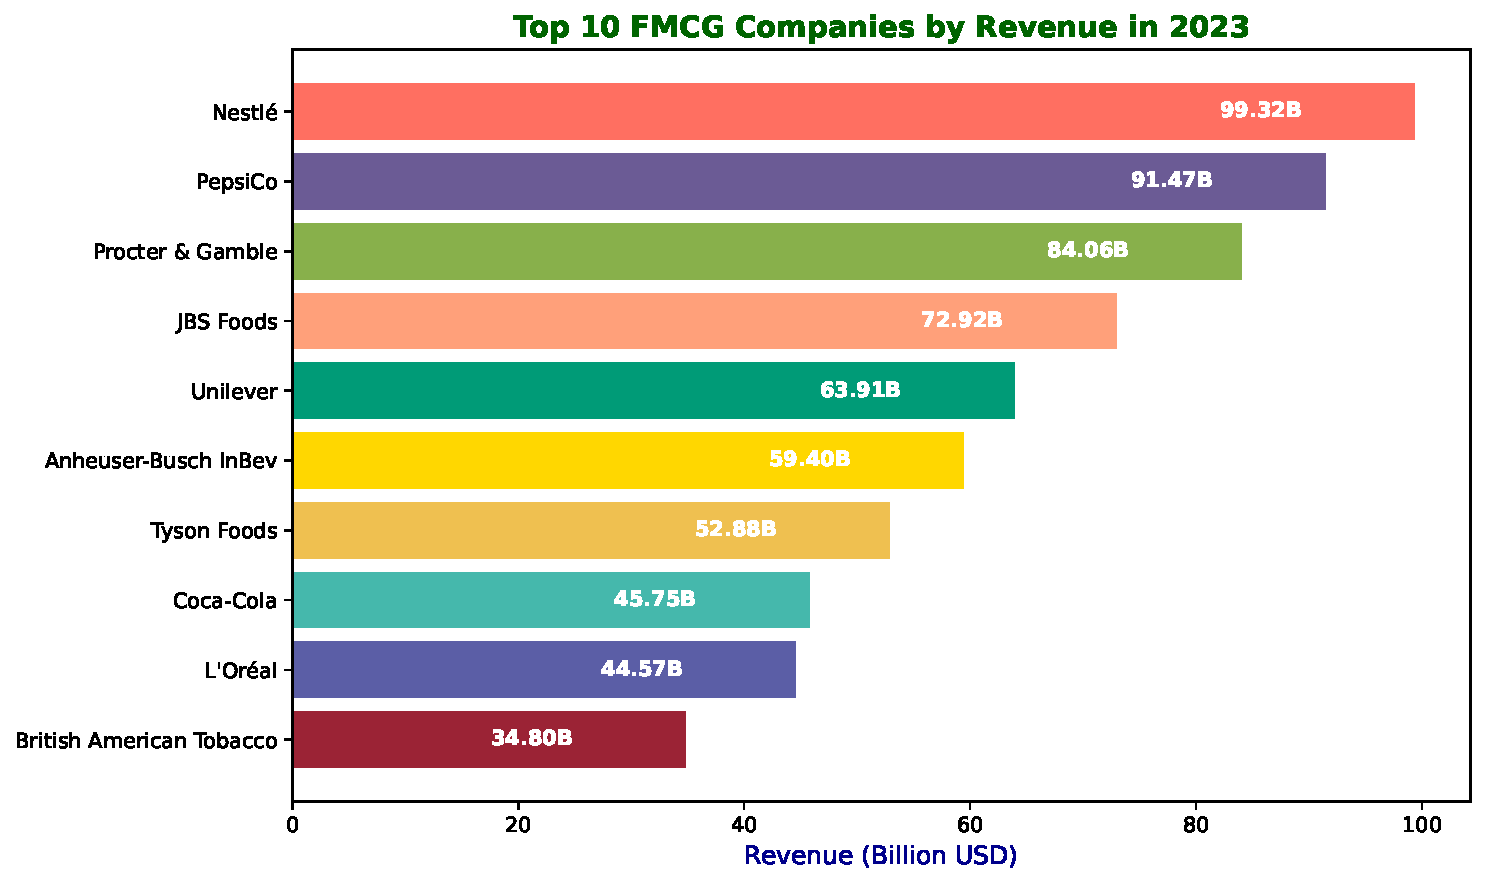
\includegraphics[keepaspectratio]{_thesis_files/figure-pdf/fig-consumer-goods-output-1.pdf}}

}

\caption[Consumer Goods]{\label{fig-consumer-goods}Consumer Goods}

\end{figure}%

In China, while there are signs of young Chinese consumers valuing
experiences over possessions, the raw sales growth numbers show
consumerism is only increasing (Claudio-Quiroga et al., 2025; Hui et
al., 2025; Y. Jiang, 2023; X. Zhang, 2025).

\subsubsection{Clothes and the (Fast) Fashion
Industry}\label{clothes-and-the-fast-fashion-industry}

Just like Fast-Moving Consumer Goods, fast fashion operates with low
margins and follows consumer trends. Young people are the largest
consumers of fast fashion ({``Young {Consumers}' ({Complicated}) {Love
For Fast Fashion In} 3 {Stats},''} n.d.). (In European Environment
Agency, 2022 European Environment Agency (EEA)) estimates based on trade
and production data that EU27 citizens consumed an average 15kg of
textile products per person per year. (Textile Exchange, 2021) Fashion
industry revenue is above USD 1.5 trillion; COP26 policy calls for 45\%
cut in emissions by 2030. The European Commission wants to reduce the
impact of fast fashion on EU market (ERR, 2022). There are also other
local policy initiatives aiming to tackle the waste problem. For example
the New Standard Institute's proposed \emph{``Fashion Act''} to require
brands doing business in New York City to disclose sustainability data
and set waste reduction targets (Emily Chan, 2022b). In California, the
\emph{``Garment Worker Protection Act''} covers 45000 garment workers
with wage and safety safeguards (\emph{Lily {\textbar} Mindful + Active
Living on {Instagram}}, n.d.).

In terms of total figures, the 2.4 Trillion USD fashion industry
contributes 2\%-8\% of total global green house gas (GHG emissions);
100B USD is lost to lack of recycling; contributes 9\% of microplastics
(Adamkiewicz et al., 2022). ({``New {Standard Institute},''} n.d.)
similarly estimates the apparel \& footwear account for \textgreater{} 8
\% of global GHG and could rise up to 60\% by 2030.\\
(Centobelli et al., 2022) reports fashion industry year uses 9B cubic
meters of water, 1.7B tonnes of CO\textsubscript{2}, 92 million tonnes
of textile waste. (Emily Chan, 2022c) as things stand now, fashion
companies can't be held accountable for their actions (or indeed, their
lack of action), driving calls for extended producer responsibility.
(Köhler et al., 2021) Globally 87\% of textile products are burned or
landfilled after 1st consumer use. (Millward-Hopkins et al., 2023) shows
how 50\% of the textile waste in the UK is exported to other countries,
often to be dumped as trash in landfills or burned. (Tian Macleod Ji,
2024) found fast fashion propels 26 million tons of clothing in China's
landfills annually. In Ghana, research across several dumpsites revealed
up to 12\% of the landfill consisted of textile waste (Gyabaah et al.,
2023). The ({``Clean {Clothes Campaign},''} n.d.) decries how
\emph{``{[}t{]}he mainstream fashion industry is built upon the
exploitation of labor, natural resources and the knowledge of
historically marginalized peoples''}; in 2018, 3/5 of the 100 billion
garments produced globally ended up in landfill within one year of sale.
(FashionChecker, 2023) reports none of the top global apparel brands
pays a living wage; 60\% of garment workers are women earning below-men
wages. Yet, for certain countries this production is crucial; the
Bangladesh Garment Manufacturers and Exporters Association reports 24\%
annual growth in global market and makes up a whopping 81\% of the
exports of the country (\emph{{BGMEA} {\textbar} {Home}}, n.d.; Daily
Sun, 2022).

It's hard to make improvements to a system in an opaque environment.
(Emily Chan, 2022a) writes there's not enough transparency in the
fashion industry - greenwashing is prevalent - and introduces Fashion
Revolution's Fashion Transparency Index, in order to tackle the very
issues mentioned above (Fashion Revolution Foundation, 2022). Similarly,
(Wikirate, 2022b) presents itself thus: \emph{``Among the Index's main
goals are to help different stakeholders to better understand what data
and information is being disclosed by the world's largest fashion brands
and retailers, raise public awareness, educate citizens about the social
and environmental challenges facing the global fashion industry and
support people's activism''}. Already in 2018, Sourcemap launched the
\emph{``Open Apparel Registry''}, a crowd-sourced digital map of apparel
factories, creating a standardized database of factory names and
addresses to enhance supply-chain transparency (Mowbray, 2018).
Sustainable fashion company evaluations platform Good On You rated 5821
brands in 2023; yet most large labels with climate targets publish no
progress data (Good On You, 2023). The Fossil-Free Fashion Scorecard
graded 43 brands; 15 scored ``F'' and the sector average was a ``D''
(Stand.earth, 2023). Making use of these indexes, YouTuber
(imperfectidealist, 2020) proposes a 7-step checklist to help consumers
spot greenwashing, focused on transparency, such as if the producer has
published a full list of suppliers. While consumer understanding of
sustainability is growing, it's not necessarily very specific; for
example (Mabuza et al., 2023) shows consumer knowledge of the effects of
apparel coloration is very limited.

Nonetheless, change is happening. Qima, a company which provides
inspection and certification services for the fashion industry, found
that in 2023 inspection demand for products coming from China rose 5.4\%
year-on-year, specifically 13\% from the US, 27\% from Germany, 32\%
from the UK, and 69 \% from Mexico, demonstrating the global nature of
the business, while \emph{near-shoring} and \emph{re-shoring} accounted
for 10\% of the U.S. and EU-based buyers' procurement, underscoring the
growing need for supply chain visibility and adaptability (QIMA, 2024).
One example of a blockchain-based fibre-to-garment traceability
solution, live with 100+ brands, is (\emph{Textile {Genesis}}, n.d.);
other blockchain-based approaches are discussed at length in a dedicated
section.

There's a growing know-how on how to design sustainable fashion and
which materials to use; for instance the \emph{``Handbook of Footwear
Design and Manufacture''} includes a special chapter on green design
specifically for shoes (Leung \& Luximon, 2021). The \emph{``Circular
Design HOW''} toolkit launched 2021 to guide Baltic designers in
cradle-to-cradle approaches for circular textiles (Eesti Disainikeskus I
Estonian Design Centre, 2021). Estonian Academy of Arts' sustainable
fashion open course reached 9 European universities in 2022, covering
eco-materials and ethical sourcing (Eesti Kunstiakadeemia, 2022). And
certainly there are many more examples globally.

However, for ethical fashion practices to reach scale, materials do
matter a lot. (Textile Exchange, 2023) reports global fibre output
reached 116 million tonnes in 2022; polyester alone was 54\% percent of
the total. Access to better materials is crucial and industry
collaboration can raise the bar for everyone, such as the Better Cotton
Initiative (Better Cotton, 2023). One example of an ethical brand is
({``Sheep {Inc}. - {Softcore Radicals},''} 2023), which promises to
sequester 14kg of CO\textsubscript{2}eq per kg of wool (footprint per
finished sweater is 0.04 kg CO\textsubscript{2}eq), by using wool from
Merino sheep with regenerative practices. Robert Gentz, the Co-CEO and
co-founder of Zalando, a large European online retailer, says fast
fashion must disappear within the next decade (citing 40\% of wardrobes
are never worn), launching a separate brand called Zign, built around
sustainable materials and ethical production practices, with at least
20\% recycled content and 50\% eco-friendly materials per item
(Remington, 2020; Storbeck, 2021). Improved technology for recycling is
in the pipeline; for example (Infinited Fiber, 2023; Karila, 2024)
produces a premium fiber called Infinna, using its pulp-to-fibre
recycling tech, from waster materials - and is being used by sustainable
brands such as Patagonia.

The story of Patagonia has inspired many to see that a financially
successful, eco-friendly fashion business is a possibility; yet
Patagonia's 1 \% for the Planet pledge that has delivered about USD 140
million to grassroots environmental groups since 1985, seems like a drop
in the bucket compare to the scale of the problem (Chouinard, 2005). The
``Generation Rewear'' documentary documents the strides newer
sustainable fashion brands are making; yet a survey made for the film
showed 64\% of UK consumers wear items only once, leading to 350000
Tonnes of clothing landfilled yearly (Vanish UK, 2021).

Digital Product Passports will be mandatory for fashion under EU
Eco-design and EPR rules between 2026 and 2030, enabling ethical
shopping ({``Transparency and Sustainability Platform - {Renoon},''}
2023). New apps make alterations and repairs made easy: SOJO
door-to-Door service raised USD 2.4 million pre-seed funding for a
clothes repairs service, cutting waste and emissions (\emph{{SOJO} -
Door-to-Door Clothing Alterations and Repairs}, 2023).

\subsubsection{The (Fast) Food Industry}\label{the-fast-food-industry}

Food production is a large greenhouse gas emitter. Global warming causes
droughts and extreme weather, wars and conflicts, which in turn
increases the volatility in food prices (Eshe Nelson et al., 2023).
(Nabipour Afrouzi et al., 2023) reports the agricultural sector
contributes approximately 25\% of the total CO\textsubscript{2}
emissions and 13.5\% of the total global anthropogenic greenhouse gas
emissions. (Poore \& Nemecek, 2018) suggests a slightly higher 26\% of
carbon emissions come from food production. (Saner et al., 2015) reports
dairy (46\%), meat and fish (29\%) products making up the largest GHG
emission potential. Livestock products (meat) are 15\% of agricultural
foods valued at €152 billion in 2018 globally (A. S. Patel et al.,
2023). (J. L. Bailey \& Eggereide, 2020) shows how the Norwegian
government plans to increase salmon production 5x by 2050; the demand
for food is increasing.

Re-designing the industrial food systems for an increasing global
population is a challenge - yet improvements are possible at every step
of the way. For example, an Italian retail supermarkets worried about
their carbon footprint ran a pilot program, which cut food + packaging
waste emissions from 436 kg CO\textsubscript{2}eq to 339 kg
CO\textsubscript{2}eq per store per year (total 22\% emissions
reduction) (Marrucci et al., 2020). Perennial (multi-year) crops are
less carbon intensive, reducing inputs of gasoline, labor, etc (Aubrey
Streit Krug \& Yin Lu, 2023), yet large agritech companies like Monsanto
rely on selling seeds annually for profits putting them at odds with
perennial crops; single-year seeds have led to farmer suicides when
crops fail in poor communities.

Supply chain innovation in food industries may enable more transparency.
Provenance and traceability of food has implications for sustainability
and health. Food fraud is a contentious issue which requires new
science- and legislation-based solutions. One example is \emph{fake
honey}, meaning synthetic honey, or actual honey fraudulently blended
with cheaper sugar syrup, which can pass some laboratorty tests,
requiring improved technology, such as DNA-analysis to find real honey
(ERR, 2023; X. Song et al., 2020). China is the world's largest honey
producer, making about 24\% of world total (Food and Agriculture
Organization of the United Nations, 2023) and has been implicated in
tampering with their product. Apimondia, the International Federation of
Beekeepers' Associations, canceled its annual honey award because of
wide-spread supply-chain fraud, as they were unable to guarantee the
authenticity of honey (Ungoed-Thomas, 2024). The same is true for cocoa
beans, which are at high risk from food fraud (E. Fanning et al., 2023).

Complex supply chains make seafood (marine Bivalvia, mollusks) logistics
especially prone to fraud, leading to financial losses and threats to
consumer health (Santos et al., 2023). (C.-H. Chang et al., 2021)
\emph{fish fraud} is a large global problem but it's possible to use
DNA-tracking to prove where the fish came from. In Taiwan, the 27 KURA
SUSHI branches sold more than 46 million plates of sushi in 2019.
Illegal, unreported and unregulated fishing (IIU) fishing is widespread;
the EU is adopting countermeasures (D. E. Kim \& Lim, 2024).
Likewise,(Katie Gustafson, 2022) proposes a \emph{``Uniform traceability
system for the entire supply chain''} for seafood and (Mamede et al.,
2022) proposes fingerprinting of Sea Urchin for seafood tracing.

In total, the world consumes around 200 million tonnes of fish and
seafood every year, including wild catch and aquaculture (fish farming)
(Ritchie \& Roser, 2021). Precise and recent data about the fishing
industry is hard to come by. However, by some estimates, industrial
fishing accounts for approximately 75\% of the entire global catch, the
rest being artisanal fishing; 26\% of the catch is caught using bottom
trawling and dredges, which are highly damaging to the natural
environment; and 10-12\% using mid-water (pelagic) trawls, which are
somewhat less intrusive; around 20-30\% of the fish is caught using
large nets; around 6-7\% using industrial longlines (both surface level
and deep-set); and the rest is caught using a variety of other fishing
gear (Amoroso et al., 2018; Cashion et al., 2018; Hilborn et al., 2023;
Jacquet \& Pauly, 2022). About 10.8 \% of total catch is discarded;
bottom-trawling alone accounts for 46\% of discards (Pérez Roda et al.,
2019). (Muñoz et al., 2023) calls for banning of bottom trawling. (Sala
et al., 2021) notes that only 2.7\% of the world ocean is highly
protected and calls for a globally coordinated effort to protect marine
biodiversity.

Given these statistics, (Springmann et al., 2021) proposes veganism is
the most effective decision to reduce personal CO\textsubscript{2}
emissions. The food sovereignty movement, born in the late 1990s,
champions everyone's right to healthy and sustainable food, focusing on
\emph{local food systems} to bring producers and consumers closer
together, planting seeds and growing food in the cities, countryside,
and even indoors (Stall-Paquet, 2021). In a similar vein, the \emph{Farm
to Fork} European Union policy proposes to \emph{shorten the supply
chain} (meaning less change for fraud and less emissions) from the
producer to the consumer and add transparency to the system (Financial
Times, 2022). In Japan, one startup in this space is ``Secai Marche'',
self-described as ``Asia's Food Supply Chain'', operating a cold chain
and fulfillment platform, connecting farmers across Japan and Southeast
Asia to more than 500 retailers, deliverling over 4000 distinct products
(SKUs), including vegetables, fruits, eggs, seafood, across its
transparent system, with AI-based demand-forecasting and optimized
truck-routing (Catherine Shu, 2023).

However, a local Taiwanese study refutes the idea that local
\emph{``farm-to-fork''} sourcing is greener in terms of carbon footprint
and environmental impacts; taking a case-study of ice-cream production
in Taiwan, the authors finds sourcing ingredinents from local,
small-scale farming in Taiwan, is more carbon-intenstive in comparison
with ingredients imported from large-scale industrial farms in New
Zealand and Sri Lanka, even if accounting for the higher transportation
emissions (Y.-C. Huang et al., 2025).

(Lulovicova \& Bouissou, 2023) apply a territorial life cycle approach
to evaluate local food policies in Mouans Sartoux, France, and
demonstrate that simply reducing food miles is not enough to ensure a
lower environmental footprint; the biggest drivers of total impact are
changes in farm practices, aggregation methods, retail infrastructures,
and procurement contracts, rather than proximity alone - local supply
chains can outperform global chains \emph{if} local food policies
combine geographic proximity with improvements in on-farm efficiency,
logistics, energy use, and local retail systems, to realize true
sustainability gains.

It comes down to \emph{what} is compared to \emph{what}.

A local Taiwanese vertical farm, ``Yes Health iFarm'' (largest indoor
vertical farm in Asia as of 2018), spans a 15 stories and employs 130
staff; they use LED lighting tailored to specific plant type, growing 30
varieties of edible plants (e.g.~arugula, ice plant, mustard leaf, etc),
with high quality and `distinctive crunch and flavor'; the yield is 100
times larger than in traditional farming, while using only 1/10 of the
water; the factory is extremely clean, with zero pesticide residues,
zero heavy metal contamination, zero parasites, zero e coli, low
nitrates, low bacteria - demonstrating a high-tech driven approach can
provide exceptional resource efficiency and quality (Renée Salmonsen,
2018).

Even when problems with food are discovered, solutions might take years
to emerge. For example, IARC (International Agency for Research on
Cancer) warns aspartame (artificial sweetener found in many soft drinks)
could cause cancer, confirmed by 2 separate studies; yet the
international standards for aspartame have yet to be updated 2 years
later (J. Fu, 2024; Riboli et al., 2023; Rigby, 2023).

Food is also about cuisine and culture; foods become popular if we hear
stories and see cuisine around a particular crop (Aubrey Streit Krug \&
Yin Lu, 2023). Food is about enticing human imagination and taste buds.
That is to say, improving food systems is not only about technical
details. Culture, community, cuisine, and storytelling can all play a
part to have better quality food and reduce food waste. While perhaps
over-romanticizing mushrooming, Anna Lowenhaupt Tsing's ethnographic
exploration in her book about the matsutake mushroom illustrates how
foragers and distributors collaborate across damaged ecosystems to
sustain a cross-border commodity chain becoming a sign of ecological
resilience, where disturbed forests altered by logging and industrial
activities; mushrooms form a ``gift economy'' that connects rural
pickers in Oregon, Japan, China, and Finland with affluent urban
consumers around the world; the price is high due to the foraging nature
of the collection (some sources call it the most expensive mushroom in
the world, sold at over \$1000 USD per kg, no intensive farming
practices involved); the author believes this is a type of collaboration
that does not depend on endless economic growth (personally, I would
describe it as economics of luxury goods) - in any case, it does remind
us that cultural narratives and local know-how (e.g.~cultural products)
do influence food and \emph{perhaps} can play a small part in more
resilient and sustainable food systems (Remley, 2025; Tsing, 2015; X.
Yang et al., 2008).

Coming back to apps, there are several initiatives aimed at reducing
food waste by helping people consume food that would otherwise be thrown
away, including Olio and Too Good To Go.

\begin{figure}[H]

{\centering 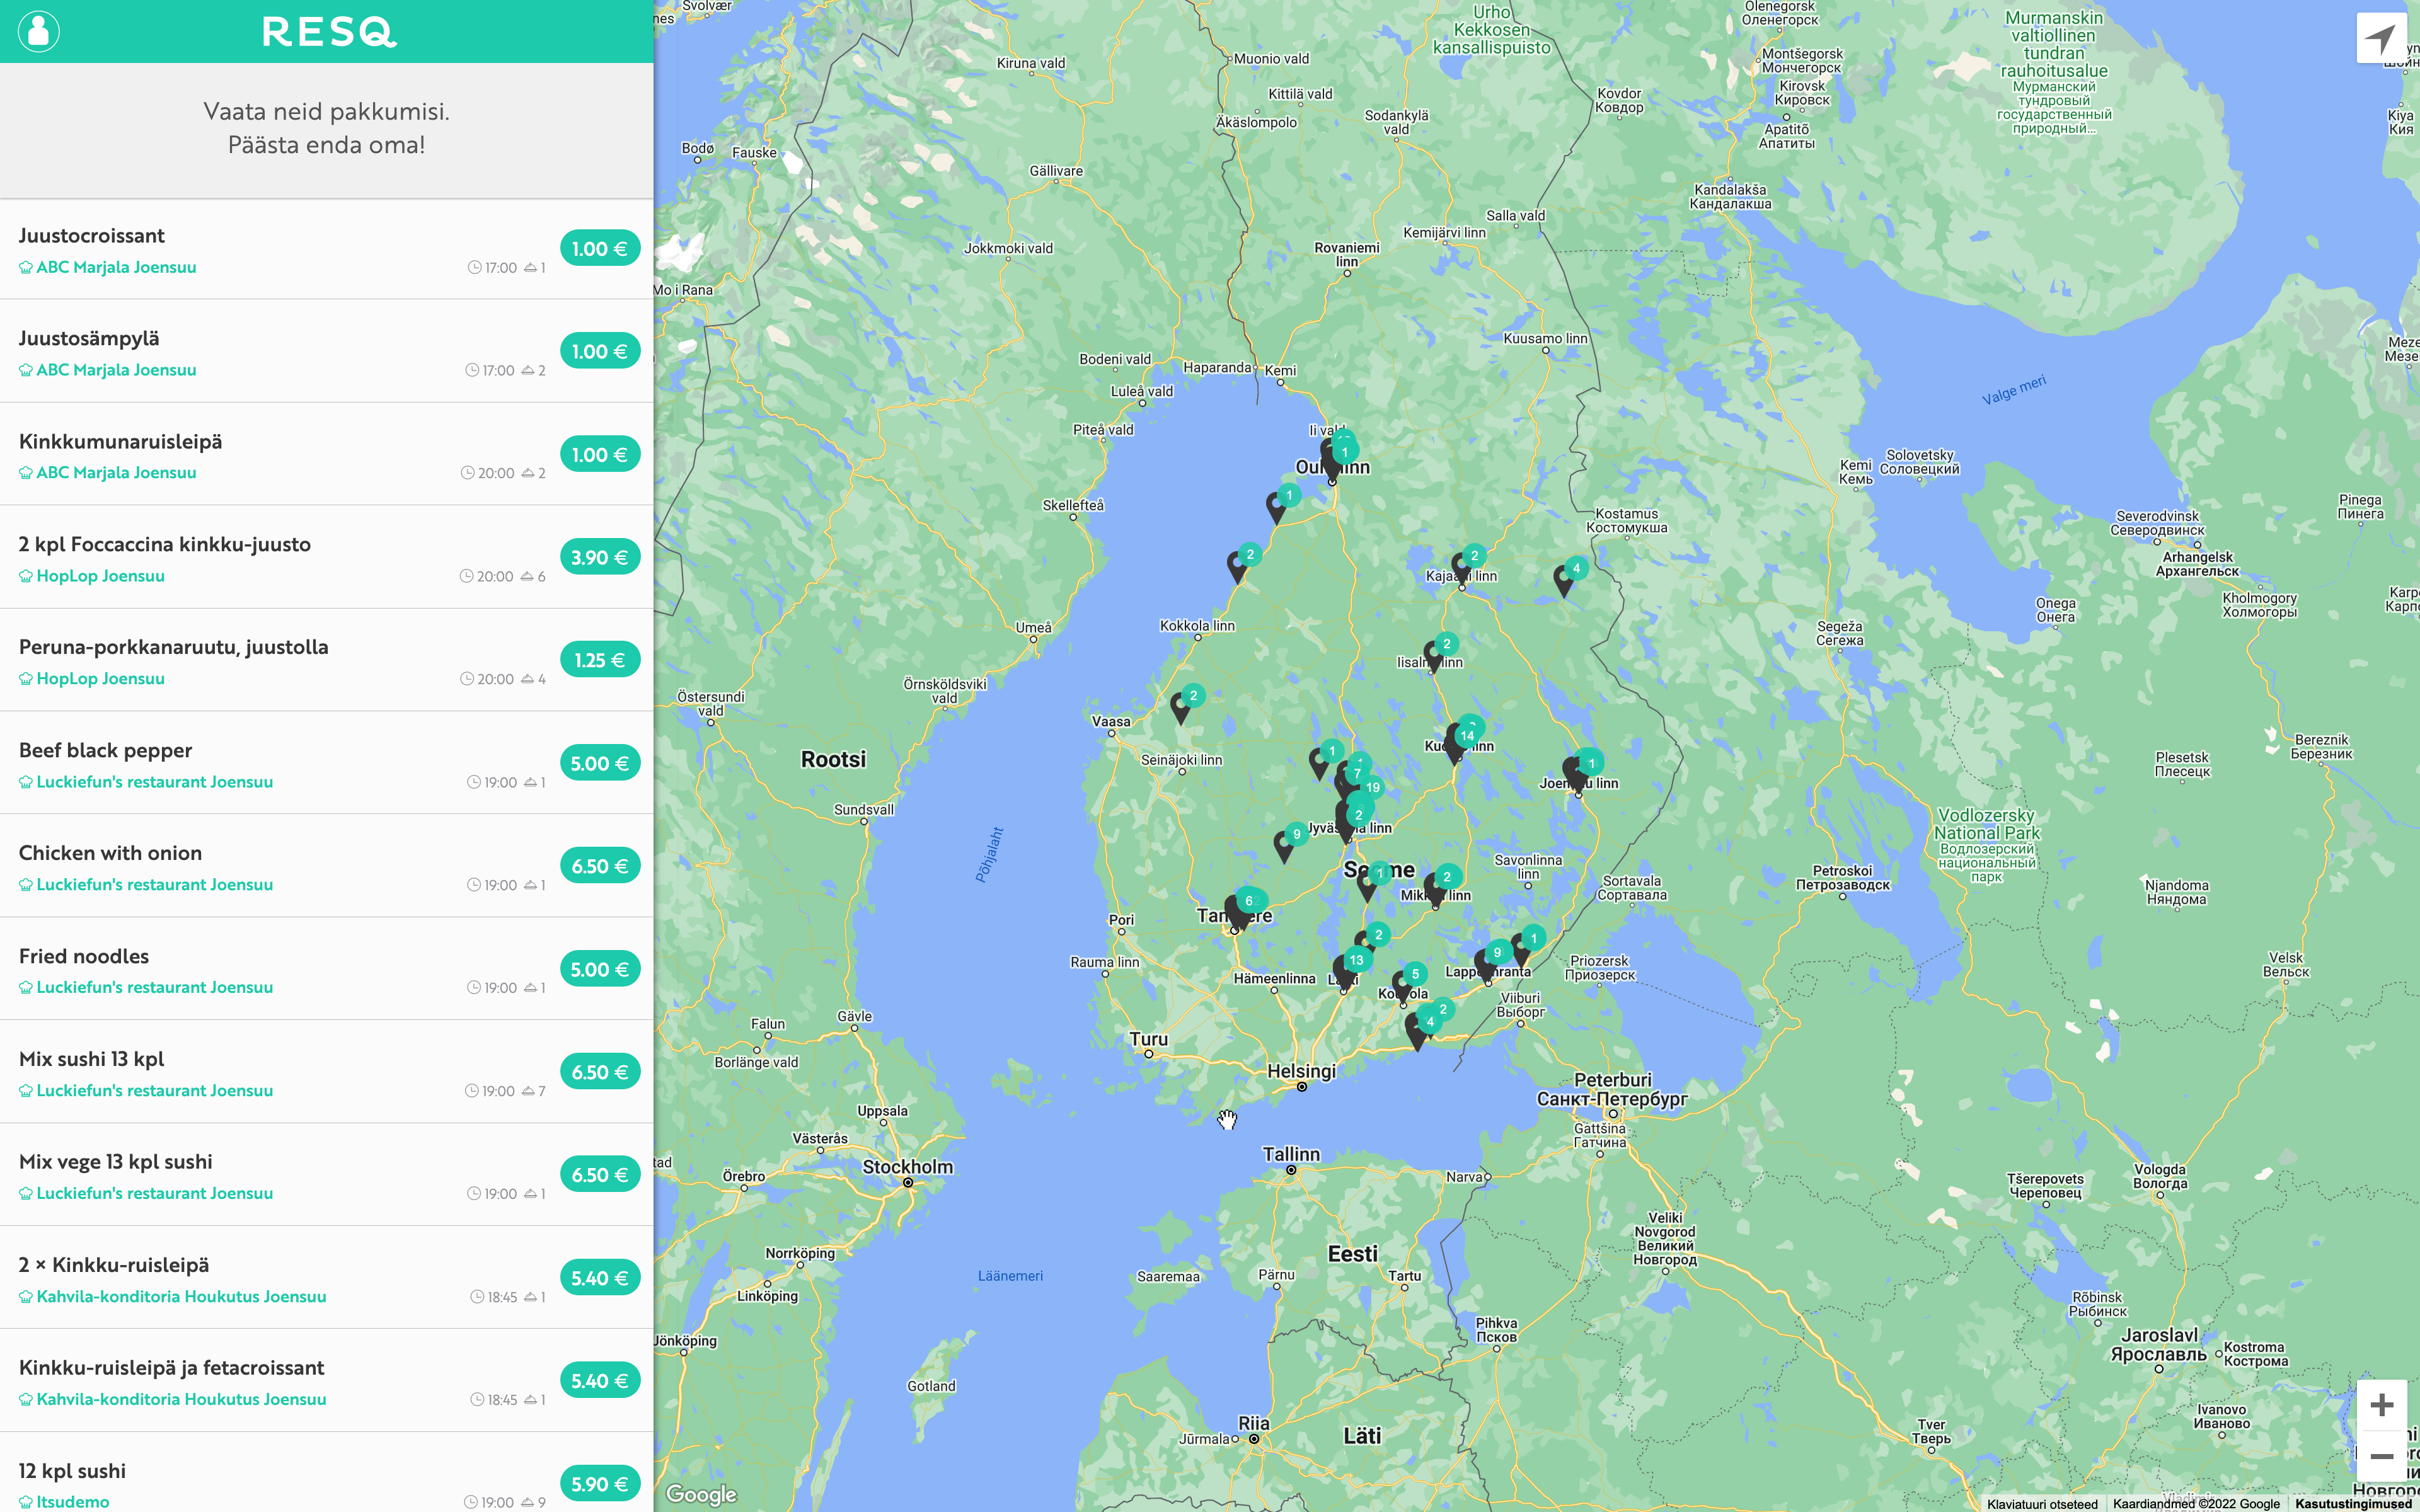
\includegraphics[width=1\linewidth,height=\textheight,keepaspectratio]{./images/design/resq-club.png}

}

\caption{ResQ Club saves food waste by selling left-over foods cheaply}

\end{figure}%

\def\pandoctableshortcapt{Food Saving Apps}

\begin{longtable}[]{@{}
  >{\raggedright\arraybackslash}p{(\linewidth - 2\tabcolsep) * \real{0.3611}}
  >{\raggedright\arraybackslash}p{(\linewidth - 2\tabcolsep) * \real{0.6389}}@{}}
\caption[Food Saving Apps]{Food saving apps}\tabularnewline
\toprule\noalign{}
\begin{minipage}[b]{\linewidth}\raggedright
Name
\end{minipage} & \begin{minipage}[b]{\linewidth}\raggedright
Description
\end{minipage} \\
\midrule\noalign{}
\endfirsthead
\toprule\noalign{}
\begin{minipage}[b]{\linewidth}\raggedright
Name
\end{minipage} & \begin{minipage}[b]{\linewidth}\raggedright
Description
\end{minipage} \\
\midrule\noalign{}
\endhead
\bottomrule\noalign{}
\endlastfoot
Karma & \\
ResQ Club & (Kristina Kostap, 2022) ResQ Club in Finland and Estonia for
reducing food waste by offering a 50\% discount on left-over restaurant
meals before they are thrown away. \\
Kuri & (Haje Jan Kamps, 2022) Less impact of food \\
Social media groups (no app) & \\
\end{longtable}

\let\pandoctableshortcapt\relax

As with any contentious issue, when it comes to food, people have
differing points of view. (Eriksson et al., 2023) discusses best
practices for reducing food waste in Sweden and (Röös et al., 2023)
identified 5 perspectives in a small study (n = 106) of views on the
Swedish food system.

\def\pandoctableshortcapt{Perspectives on the Food Systems in Sweden}

\begin{longtable}[]{@{}
  >{\raggedright\arraybackslash}p{(\linewidth - 2\tabcolsep) * \real{0.3611}}
  >{\raggedright\arraybackslash}p{(\linewidth - 2\tabcolsep) * \real{0.6389}}@{}}
\caption[Perspectives on the Food Systems in Sweden]{Perspective on food
systems in Sweden from (Röös et al., 2023).}\tabularnewline
\toprule\noalign{}
\begin{minipage}[b]{\linewidth}\raggedright
Perspective
\end{minipage} & \begin{minipage}[b]{\linewidth}\raggedright
Content
\end{minipage} \\
\midrule\noalign{}
\endfirsthead
\toprule\noalign{}
\begin{minipage}[b]{\linewidth}\raggedright
Perspective
\end{minipage} & \begin{minipage}[b]{\linewidth}\raggedright
Content
\end{minipage} \\
\midrule\noalign{}
\endhead
\bottomrule\noalign{}
\endlastfoot
\emph{``The diagnostic perspective''} & ``\emph{All hands on deck to fix
the climate''} \\
\emph{``The regenerative perspective''} & ``\emph{Diversity, soil health
and organic agriculture to the rescue''} \\
\emph{``The fossil-free perspective''} & ``\emph{Profitable Swedish
companies to rid agriculture and the food chain of fossil fuel''} \\
\emph{``The consumer-driven perspective''} & \emph{``A wish-list of
healthy, high-quality and climate-friendly foods''} \\
``The hands-on perspective'' & ``Tangible solutions within the reach of
consumers and the food industry'' \\
\end{longtable}

\let\pandoctableshortcapt\relax

\subsection{In Practice: Sustainability Begins in
Software}\label{in-practice-sustainability-begins-in-software}

Humans live in artificial environments where \emph{most things} are
designed by humans. Design encompasses most everything in our daily
lives. The \emph{experiences} we take part in are increasingly created
based on some type of data. \emph{Digital Sustainability} refers to the
idea that \emph{digital} enables \emph{sustainability}. Information
pertaining to emissions would flow through the economy not unlike the
carbon cycle itself.

Designing user interfaces for sustainable interactions means
incorporating data and tools to enable designers to make decisions which
reduce the emissions of their designs. Software is key to building more
sustainable products, already for decades (B. B. Gupta et al., 2023).
Increasingly, AI-assisted design is where sustainability starts: AI
provides the parameters for sustainability. Companies like AutoDesk have
introduced CO\textsubscript{2e} calculations inside their design
software, helping designers reduce material usage, energy consumption,
CO\textsubscript{2e} emissions, while increasing potential for reuse and
recyclability (Mike Haley, 2022). As AI tools and data quality improve,
a increasing number of parameters for deciding the suitable life cycle
design, will become available (Singh \& Sarkar, 2023).

(Pan \& Nishant, 2023) proposes 6 dimensions of \emph{AI} usage in
\emph{digital sustainability}. The chart is purely illustrative to
highlight the value of AI for sustainability; it's not based on numeric
metrics.

\begin{figure}

\centering{

\pandocbounded{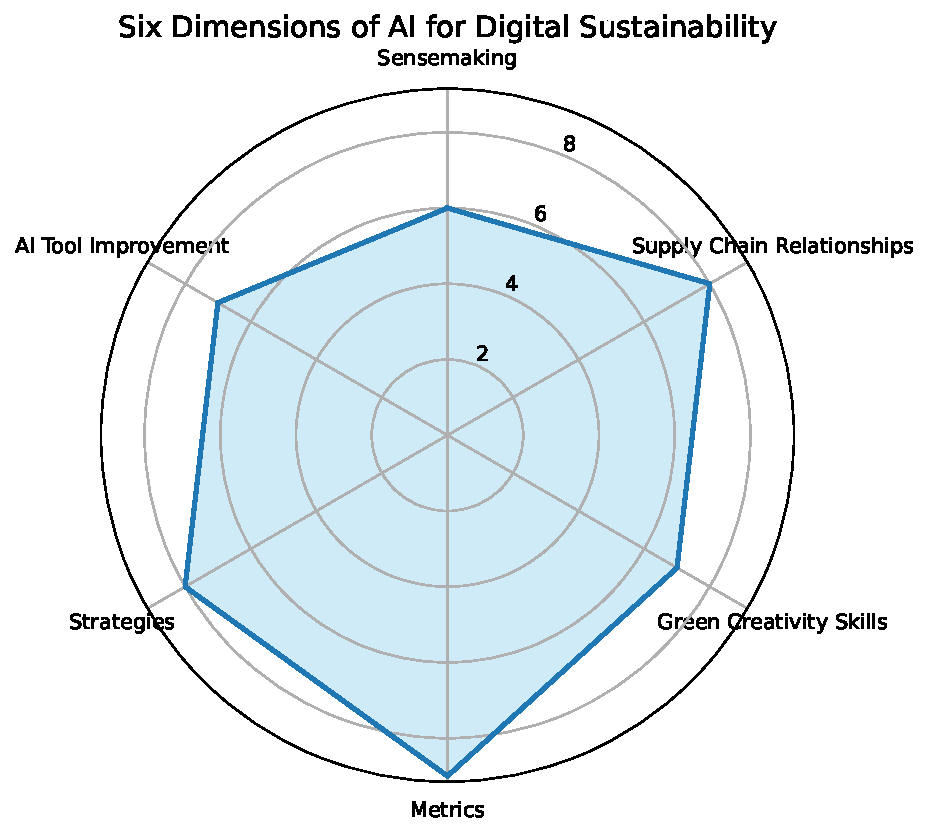
\includegraphics[keepaspectratio]{_thesis_files/figure-pdf/fig-ai-sust-six-output-1.pdf}}

}

\caption[AI Use in Sustainability]{\label{fig-ai-sust-six}AI Use in
Sustainability}

\end{figure}%

A crucial part of digital product design are \emph{design systems} to
keep consistency across the experience, and allowing teams to work
together towards a shared goal. Design systems accelerate development
and foster a cohesive user experience across products by reducing design
debt (M. Suarez et al., 2020). Yet the latest (Zeroheight Team, 2025)
survey (n = 294) shows that over 53\% of design systems are minimally
automated or not automated at all - and only 10\% of the designers
actively use AI, with 36\% having experimented with AI-driven design.
AI-usage for design across industry is uneven. Designers working at
Google have been designing in collaboratiom with AI for a while and
already in 2019 published the People + AI Guidebook, outlining best
practices for designing with AI - to make human-centered AI products
(\emph{People + {AI Guidebook}}, n.d.). In the enterprise context,
(Zimmerman et al., 2021) delves into the proposition of UX designers as
pioneers pushing AI-based adaptive UIs, as UX designers are the ones who
will best notice the broken workflows. All these findings underline,
there's still work to be done for the broader field of design to adopt
AI-based solution. Education is of the key, and one proposed path is
involving more young HCI designers in AI-oriented workshops to support
them building the future of UI/UX with AI (Battistoni et al., 2023).

\subsubsection{Data-Driven Design}\label{data-driven-design}

I believe it's possible to learn from the growth of digital platforms
and superapps to see how data-driven design could enable sustainability
to become mainstream. Sustainability touches every facet of human
existence and is thus an enormous undertaking. Making progress on
sustainability is only possible if there's a large-scale coordinated
effort by humans around the planet. For this to happen, appropriate
technological tools are required - simplifying the complexity of
sustainability.

Digital platforms are focused on \emph{growth design}, how to
\emph{attract} and \emph{retain} users. Superapps are the latter stage
of the economies of digital platforms, where previously vertically
targeted apps expand horizontally to provide an ever-increasing number
of services. For digital products (including superapps) the main
application of interaction design is for \emph{growth} in usage, how to
get more people (user journey and conversion funnels) to use the product
i.e user acquisition, retention, engagement, and monetization and keep
using it (retention and engagement), often optimizing on-boarding,
features, and personalization (Kende, 2023; Steger, 2019).

Platform economy companies popularized and expanded \emph{data-driven
design} in the service of growth marketing (also known colloquially as
\emph{growth hacking}). Capturing user data was part of this strategy
which enabled improving the products. Digital product design is
increasingly data-driven and digital platforms operate \emph{design as a
process} in a continuous feedback loop, where \emph{measurements},
\emph{experiments}, predictive analytics and personalization form a
data-drive design culture. As we humans go about our daily business,
governments and companies track our activities using various
technologies, which produces massive amounts of user interaction data.

Platform economy companies are the capture and use large amounts of data
from users. Data is useful for designing better products. Designing for
high retention (users keep coming back). Network Effects, the more
people use a platform, the more valuable it becomes. Platforms that
continuously add features (provided consumer legislation allows it) may
eventually evolve into superapps, which are useful for providing
services for a wide category of human needs. Bundling many services
under one super-brand. Superapps are possible thanks to Nudge, Economies
of Scale, Network Effects, Behaviour Design. Large Digital Platforms
have a very small number of workers relative to the number of users they
serve. This creates the necessity for using automation for both
understanding user needs and providing the service itself. Creating a
good product that's useful for the large majority of users depends on
\emph{Data-Driven Design.}

Design is as much about how it works as it's about the interface. There
are many approaches to design - from playful to practical to critical
and to data-driven. Nonetheless, many types of design share a common
goal designing for a good \emph{user experience} - except for those
design fields looking for \emph{shock value}. Digital product design can
be seen as a specific discipline under the umbrella of \emph{experience
design}. In (Michael Abrash, 2017) Laura Fryer, Meta Oculus augmented
reality incubation general manager, says as much: \emph{``People buy
experiences, not technology.''}

Personalization is the key to growth. The largest businesses today
(measured in number of users) design the whole user experience in order
to reach \emph{Scale}. Social apps require personalization because a
personal user experience will increase \emph{trust} and \emph{k-factors}
(sharing and inviting your friends) (Baron, 2023; B. Kim, 2023).
Intelligent Interfaces use interaction design to provide relevant and
personalized information in the right context and at the right time.
Popular consumer platforms strive to design solutions that feel
personalized at every touch point on the user journey (to use the
language of service design) at the scale of hundreds of billions of
users. Businesses care about Total addressable market (TAM), serviceable
addressable market (SAM), target audience (TA), and use hypothesis and
validation for iterating on features, to reach these lofty goals.

\subsubsection{Circular Design for a Circular
Economy}\label{circular-design-for-a-circular-economy}

The bible for Circular Economy, the \emph{``Cradle to Grave''} book was
released over 2 decades ago; change is slow, but change is happening
(McDonough \& Braungart, 2002).

Circular design is only possible if supply chains become circular as
well. (Hedberg \& Šipka, 2021) argues digitization and data sharing is a
requirement for building a circular economy. Yet, sometimes technology
fails. Nonetheless, many current technological hurdles can be overcome
by supply chain professionals who are experts in connecting supply
streams (Dull, 2021). (Oikos Denktank, 2021) argues circular design
requires new skills, one of which is circular material procurement.

To take a specific industry, digitization of mining systems allows
enhance the reliability of supply chains, and provides better supply
chain transparency (CRM Alliance, 2020). This does not only include
tracking the critical raw materials, but also the social aspects
surround the mine. While this rarely makes the international media,
(Eerola, 2022) maps 20 ongoing mining and mineral-exploration disputes
in Finland, calling for systematic dispute monitoring, in order to
maintain a social license to operate.

The complexity of resource and delivery networks necessitates more
advanced tools to map supply chains (Knight et al., 2022). The COVID19
pandemic - and resulting blockages in resource delivery - highlighted
the need to have real-time visibility into supply chains (Finkenstadt \&
Handfield, 2021). Moreover, in the context of the EU Plastics Strategy,
\emph{``the European Commission has launched a pledge to increase the
use of recycled content to 10 million tons by 2025''}.

Already in 2020, a company founded to solve these exact issues,
Circularise, funded in part by the EU Commission H2020 SME Instrument,
developed a privacy-focused blockchain-based data exchange protocol for
tracing plastics across supply chains, aiming to boost transparency and
circularity across industries; their \emph{``Open Standard for
Sustainability and Transparency''} used ZK Proofs (a type of
cryptograhic verification) for privacy preservation (a requirement of
many companies), while being able to prove the data is valid
(Circularise, 2020b, 2020a). Circularise is currently the market leader
in providing \emph{Digital Product Passports}, the value of which their
tagline \emph{``Connecting the Value Chain, One Product at a Time''}
explains quite clearly; in other words, the company aims to enable
circular economies by overcoming current limitations and communication
barriers in the value chain, by using an open blockchain-based
communications protocol (Stretton, 2022a).

It's important in which structure data is stored, affecting the ability
to efficiently access and manage the data while guaranteeing a high
level of data integrity, security, as well as energy usage of said data.
Blockchains are a type of shared database where the data is stored in
several locations with a focus on making the data secure and very
difficult to modify after it's been written to the database. Once data
is written to the blockchain, modifying it would require changing all
subsequent records in the chain and agreement of the majority of
validators who host a version of the database. Blockchain is the main
technology considered for accounting for the various inputs and complex
web of interactions between many participants inside the supply chain
networks.

Several startups are using to track source material arriving to the
factories and product movements from factories to markets and there are
hundreds of paper researching blockchain use in supply change operations
since 2017 (Dutta et al., 2020). Blockchains enable saving immutable
records into distributed databases (also known as ledgers). It's not
possible to (or extremely difficult) to change the same record, only new
records can be added on top of new ones. Blockchains are useful for data
sharing and auditing, as the time and place of data input can be
guaranteed, and it will be easier to conduct a search on who inputted
incorrect data; however the system still relies on correct data input.
As the saying goes, \emph{``garbage in, garbage out''}.

There are several technologies for tracking goods across the supply
chain, from shipping to client delivery. Data entry is a combination of
manual data input and automated record-keeping facilitated by sensors
and integrated internet of things (IoT) capabilities. For example
(Ashraf \& Heavey, 2023) describes using the Solana blockchain and
Sigfox internet of things (IoT) Integration for supply chain
traceability where Sigfox does not need direct access to internet but
can send low powered messages across long distances (for example
shipping containers on the ocean). (Van Wassenaer et al., 2023) compares
use cases for blockchains in enhancing traceability, transparency and
cleaning up the supply chain in agricultural products.

\def\pandoctableshortcapt{A Sample of Blockchain-based Supply Chain
Companies}

\begin{longtable}[]{@{}
  >{\raggedright\arraybackslash}p{(\linewidth - 4\tabcolsep) * \real{0.3288}}
  >{\raggedright\arraybackslash}p{(\linewidth - 4\tabcolsep) * \real{0.3288}}
  >{\raggedright\arraybackslash}p{(\linewidth - 4\tabcolsep) * \real{0.3425}}@{}}
\caption[A Sample of Blockchain-based Supply Chain Companies]{A sample
of blockchain-based supply chain companies as of summer
2023.}\tabularnewline
\toprule\noalign{}
\begin{minipage}[b]{\linewidth}\raggedright
Company
\end{minipage} & \begin{minipage}[b]{\linewidth}\raggedright
Link
\end{minipage} & \begin{minipage}[b]{\linewidth}\raggedright
Literature
\end{minipage} \\
\midrule\noalign{}
\endfirsthead
\toprule\noalign{}
\begin{minipage}[b]{\linewidth}\raggedright
Company
\end{minipage} & \begin{minipage}[b]{\linewidth}\raggedright
Link
\end{minipage} & \begin{minipage}[b]{\linewidth}\raggedright
Literature
\end{minipage} \\
\midrule\noalign{}
\endhead
\bottomrule\noalign{}
\endlastfoot
Ocean Protocol & oceanprotocol.com & \\
Provenance & provenance.io & \\
Ambrosius & ambrosus.io & \\
Modum & modum.io & \\
OriginTrail & origintrail.io & \\
Everledger & everledger.io & \\
VeChain & vechain.org & \\
Wabi & wabi.io & \\
FairFood & fairfood.org & \\
Bext360 & bext360.com & \\
SUKU & suku.world & (Miller, 2019) SUKU makes supply chains more
transparent yet seems to have pivoted away from supply chains \\
\end{longtable}

\let\pandoctableshortcapt\relax

Electronics contain valuable materials which can be recovered.
Meanwhile, (K. Liu et al., 2023) reports e-waste is growing 3\%-5\%
every year, globally. (Thukral \& Singh, 2023) identifies several
barriers to e-waste management among producers including lack of
awareness and infrastructure, attitudinal barriers, existing
\emph{informal} e-waste sector, and the need for an e-waste license.

(Builders for Climate Action, 2021) finds embodied carbon averages 250
kg CO\textsubscript{2}eq per m² of floor area for new Canadian homes,
varying from 175-400 kg CO\textsubscript{2}eq per m² based on building
material choices; one standard house emits 32--75 t
CO\textsubscript{2}eq; the authors believe however, using \emph{biogenic
materials} (e.g.~naturally grown materials including wood, bamboo,
straw, hemp, cork, and mycelium), could make the houses carbon negative,
storing 9--60 t CO\textsubscript{2}eq emissions - enough to meet the
2030 of the entire building sector.

\subsubsection{Tracking Ethics \& Cruelty: Transparent Factories and
Supply
Chains}\label{tracking-ethics-cruelty-transparent-factories-and-supply-chains}

\begin{quote}
``Secrecy is the linchpin of abuse of power\ldots its enabling force.
Transparency is the only real antidote.'' Glen Greenwald, Attorney and
journalist. (Greenwald, 2015)
\end{quote}

In the most general sense, supply chain transparency enables stakeholder
accountability (Circularise, 2018; Doorey, 2011; J. Fox, 2007). Products
are made from resources distributed across the planet and transported to
clients around the world which currently causes high levels (and
increasing) of greenhouse gases. \emph{``Transport greenhouse gas
emissions have increased every year since 2014''} (\emph{Climate Change
Mitigation}, 2023). Freight (transport of goods by trucks, trains,
planes, ships) accounts for 1.14 gigatons of CO\textsubscript{2}
emissions as per 2015 data or 16\% of total international supply chain
emissions (Yuqing Wang et al., 2022).

\def\pandoctableshortcapt{Share of CO\textsubscript{2}eq Emissions by
Type of Transport Globally}

\begin{longtable}[]{@{}ll@{}}
\caption[Share of CO~2~eq Emissions by Type of Transport Globally]{Share
of CO\textsubscript{2}eq emissions by type of transport globally
(Statista \& IEA, 2022).}\tabularnewline
\toprule\noalign{}
Type of Transport & Percentage \\
\midrule\noalign{}
\endfirsthead
\toprule\noalign{}
Type of Transport & Percentage \\
\midrule\noalign{}
\endhead
\bottomrule\noalign{}
\endlastfoot
Passenger cars & 39\% \\
\textbf{Medium and heavy trucks} & 23\% \\
\textbf{Shipping} & 11\% \\
\textbf{Aviation} & 9\% \\
Buses and minibuses & 7\% \\
Light commercial vehicles & 5\% \\
Two/three-wheelers & 3\% \\
Rail & 3\% \\
\end{longtable}

\let\pandoctableshortcapt\relax

In shipping, (Matthew Gore et al., 2022) reports the International
Maritime Organization (IMO) targets cutting CO\textsubscript{2}
equivalent emissions in shipping 50\% by 2050 compared to 2008. In
aviation, (Platzer, 2023), a scientist working on the Apollo space
program, calls for emergency action to develop \emph{green aviation}.

(Waters, 2015) analyses the most effective strategies to improve animal
welfare and advance animal rights against a monopolistic producer
finding the most successful tactics to be (1) negotiation, (2) targeted
direct action, and (3) awareness campaigns condemning low-welfare
practices.

\subsection{Superapps Integrate Shopping, Savings, and
Investing}\label{superapps-integrate-shopping-savings-and-investing}

Superapps are the most prevalent across Asia, with China, South-East
Asia, Korea, Japan, and India leading the way, however newcomers in
Lating America and the Middle East are also making strides; meanwhile,
the US and Europe are lagging behind.

\def\pandoctableshortcapt{Global Overview of Superapps}

\begin{longtable}[]{@{}
  >{\raggedright\arraybackslash}p{(\linewidth - 14\tabcolsep) * \real{0.1250}}
  >{\raggedright\arraybackslash}p{(\linewidth - 14\tabcolsep) * \real{0.1250}}
  >{\raggedright\arraybackslash}p{(\linewidth - 14\tabcolsep) * \real{0.1250}}
  >{\raggedright\arraybackslash}p{(\linewidth - 14\tabcolsep) * \real{0.1250}}
  >{\raggedright\arraybackslash}p{(\linewidth - 14\tabcolsep) * \real{0.1250}}
  >{\raggedright\arraybackslash}p{(\linewidth - 14\tabcolsep) * \real{0.1250}}
  >{\raggedright\arraybackslash}p{(\linewidth - 14\tabcolsep) * \real{0.1250}}
  >{\raggedright\arraybackslash}p{(\linewidth - 14\tabcolsep) * \real{0.1250}}@{}}
\caption[Global Overview of Superapps]{Global overview of superapps (or
near-superapps) compiled from official company reports (IR, Press
Releases), news reports, and company websites; various metric types
(MAU, MTU, Annual Users, Customers, Registered Users) vary by company
reporting and are reduced into a single ``users'' metric for simplicity.
Each figure is sourced from official company reports, press releases, or
investor disclosures. If no recent official update was available (as in
the case of Alipay's 2020 figure), the latest known official figure is
provided. All values and dates reflect the latest data as of 2025. Data
sourced from (R. Brown, 2025; Careem, 2025; Ge \& Wei, Jul 20, 2020
06:42 PM; goto, 2023; Grab Holdings Limited, 2025; Jing, 2025; Kazanins,
2024; Laya, 2024; Philip Lee, 2025; LY Corporation, 2023; Mercado Libre,
2024; Nguyen \& Nguyen, 2023; Oost, 2024; Phocuswright, 2023; PhonePe,
2023; Pollo, 2025; Revolut, 2024b; Safaricom, 2024; Shinde, 2023, 2023;
Tecent, 2024; Verma, 2024).}\tabularnewline
\toprule\noalign{}
\begin{minipage}[b]{\linewidth}\raggedright
\textbf{App}
\end{minipage} & \begin{minipage}[b]{\linewidth}\raggedright
Origin
\end{minipage} & \begin{minipage}[b]{\linewidth}\raggedright
\textbf{Metric}
\end{minipage} & \begin{minipage}[b]{\linewidth}\raggedright
Payments (Wallet)
\end{minipage} & \begin{minipage}[b]{\linewidth}\raggedright
Savings
\end{minipage} & \begin{minipage}[b]{\linewidth}\raggedright
Investing
\end{minipage} & \begin{minipage}[b]{\linewidth}\raggedright
\textbf{Users}
\end{minipage} & \begin{minipage}[b]{\linewidth}\raggedright
\textbf{Date}
\end{minipage} \\
\midrule\noalign{}
\endfirsthead
\toprule\noalign{}
\begin{minipage}[b]{\linewidth}\raggedright
\textbf{App}
\end{minipage} & \begin{minipage}[b]{\linewidth}\raggedright
Origin
\end{minipage} & \begin{minipage}[b]{\linewidth}\raggedright
\textbf{Metric}
\end{minipage} & \begin{minipage}[b]{\linewidth}\raggedright
Payments (Wallet)
\end{minipage} & \begin{minipage}[b]{\linewidth}\raggedright
Savings
\end{minipage} & \begin{minipage}[b]{\linewidth}\raggedright
Investing
\end{minipage} & \begin{minipage}[b]{\linewidth}\raggedright
\textbf{Users}
\end{minipage} & \begin{minipage}[b]{\linewidth}\raggedright
\textbf{Date}
\end{minipage} \\
\midrule\noalign{}
\endhead
\bottomrule\noalign{}
\endlastfoot
微信 \textbf{/ WeChat (Tencent)} & China & Monthly Active Users (MAU)
combined 微信 (China) \& WeChat (International) & Yes & Yes & Yes & 1,4
billion & 2024 \\
支付寶 \textbf{Alipay (Ant Group)} & China & Annual Active Users (AAU) &
Yes & Yes & Yes & 1.3 billion & 2020 \\
美團 \textbf{Meituan} & China & Annual Transacting Users (ATU) & Yes &
No & No & 700 million & 2024 \\
\textbf{PhonePe} & India & Registered Users (Lifetime) & Yes & Yes & Yes
& 500 million & 2023 \\
\textbf{LINE} & Japan & Monthly Active Users (MAU) & Yes & Yes & Yes &
200 million & 2023 \\
\textbf{Tata Neu} & India & Members & Yes & Yes & No & 27 million &
2023 \\
\textbf{Nubank} & Brazil & Customers & Yes & Yes & Yes & 114 million &
2024 \\
\textbf{Zalo} & Vietnam & Monthly Active Users (MAU) & Yes & No & No &
75 million & 2023 \\
\textbf{Paytm} & India & Monthly Transacting Users (MTU) & Yes & Yes &
Yes & 100 million & 2023 \\
\textbf{M-Pesa} & Kenya & Active Customers & Yes & Yes & No & 34 million
& 2024 \\
\textbf{Mercado Pago} & Argentina & Monthly Active Users (MAU) & Yes &
Yes & Yes & 61 million & 2023 \\
\textbf{PicPay} & Brazil & Active Customers & Yes & Yes & Yes & 35
million & 2023 \\
\textbf{Cash App (Block)} & USA & Monthly Active Users (MAU) & Yes & Yes
& Yes & 56 million & 2023 \\
\textbf{KakaoTalk} & Korea & Monthly Active Users (MAU) & Yes & Yes &
Yes & 48 million & 2024 \\
\textbf{GoTo (Gojek/Tokopedia)} & Indonesia & Annual Transacting Users
(ATU) & Yes & Yes & Yes & 51 million & 2023 \\
\textbf{Revolut} & UK & Customers & Yes & Yes & Yes & 50 million &
2024 \\
\textbf{Careem} & UAE (Aqcuired by US-based Uber and Etisalat but still
keeps a separate brand) & Customers & Yes & No & No & 70 million &
2024 \\
\textbf{Grab} & Singapore / Malaysia & Monthly Transacting Users (MTU) &
Yes & Yes & No & 41 million & 2024 \\
\textbf{Rappi} & Colombia & Users & Yes & Yes & No & 30 million &
2023 \\
\end{longtable}

\let\pandoctableshortcapt\relax

Uber is creating an all-purpose platform for travel; only 4.1\% of rides
were electric (Levy, 2023). In the UK, Uber launched and option to book
flights, moving to a door-to-door travel solution where the same app
brings you from home to the airport, the flight, and your final
destination (Uber UK, 2023).

\def\pandoctableshortcapt{Not Quite Superapps}

\begin{longtable}[]{@{}
  >{\raggedright\arraybackslash}p{(\linewidth - 12\tabcolsep) * \real{0.1429}}
  >{\raggedright\arraybackslash}p{(\linewidth - 12\tabcolsep) * \real{0.1429}}
  >{\raggedright\arraybackslash}p{(\linewidth - 12\tabcolsep) * \real{0.1429}}
  >{\raggedright\arraybackslash}p{(\linewidth - 12\tabcolsep) * \real{0.1429}}
  >{\raggedright\arraybackslash}p{(\linewidth - 12\tabcolsep) * \real{0.1429}}
  >{\raggedright\arraybackslash}p{(\linewidth - 12\tabcolsep) * \real{0.1429}}
  >{\raggedright\arraybackslash}p{(\linewidth - 12\tabcolsep) * \real{0.1429}}@{}}
\caption[Not Quite Superapps]{Not quite super-app yet. Data sourced from
(D. C. Garcia, 2025a; Uber, 2025)}\tabularnewline
\toprule\noalign{}
\begin{minipage}[b]{\linewidth}\raggedright
App
\end{minipage} & \begin{minipage}[b]{\linewidth}\raggedright
Origin
\end{minipage} & \begin{minipage}[b]{\linewidth}\raggedright
Metric
\end{minipage} & \begin{minipage}[b]{\linewidth}\raggedright
Payments (Wallet)
\end{minipage} & \begin{minipage}[b]{\linewidth}\raggedright
Savings
\end{minipage} & \begin{minipage}[b]{\linewidth}\raggedright
Investing
\end{minipage} & \begin{minipage}[b]{\linewidth}\raggedright
Users (2025)
\end{minipage} \\
\midrule\noalign{}
\endfirsthead
\toprule\noalign{}
\begin{minipage}[b]{\linewidth}\raggedright
App
\end{minipage} & \begin{minipage}[b]{\linewidth}\raggedright
Origin
\end{minipage} & \begin{minipage}[b]{\linewidth}\raggedright
Metric
\end{minipage} & \begin{minipage}[b]{\linewidth}\raggedright
Payments (Wallet)
\end{minipage} & \begin{minipage}[b]{\linewidth}\raggedright
Savings
\end{minipage} & \begin{minipage}[b]{\linewidth}\raggedright
Investing
\end{minipage} & \begin{minipage}[b]{\linewidth}\raggedright
Users (2025)
\end{minipage} \\
\midrule\noalign{}
\endhead
\bottomrule\noalign{}
\endlastfoot
Uber & USA & Users per month & No (Only for ride-hailing) & No & No &
171 million \\
Bolt & Estonia & Lifetime users & No (Only for ride-hailing) & No & No &
200 million \\
\end{longtable}

\let\pandoctableshortcapt\relax

Superapps offer a platform with key infrastructure such as payments
already included, where ecosystem of mini-apps thrive (Heath, 2021;
Perri, 2022). Alipay, originally a payments app, has build the digital
infrastructure to provide thousands of services to billions of users
across China. 59 million people use 支小寶 (Zhixiaobao), an Al-based
assistant inside of Alipay, which can order taxis and meals, but also
interact with the Ant Bridge, Ant Ant Bridge, Ant Fortune and Ant
Insurance services inside Alipay (Finextra, 2024). (Vecchi \& Brennan,
2022) discusses the strategies Chinese apps are taking to expand to
international markets. (Giudice, 2020) finds WeChat has had a profound
impact on changing China into a cashless society, underlining how one
mobile app can transform social and financial interactions of an entire
country. (Shabrina Nurqamarani et al., 2020) discusses the system
consistency and quality of South-East Asian superapps Gojek and Grab.

Superapps are honeypots of data that is used for many types of behavior
modeling. Guido Becher from Rappi defines their super-app as
\emph{``customer-centric high frequency multi-vertical ecosystem''} this
enables cross-promotion, for example a hotel in Argentina targeted
people people who buy almond milk on Rappi with their offer of a yoga
retreat (Phocuswright, 2023; G. Suarez et al., 2021) suggests using
alternative data from super-apps to estimate user income levels,
including 4 types of data: \emph{Personal Information},
\emph{Consumption Patterns}, \emph{Payment Information}, and
\emph{Financial Services}. (Roa et al., 2021) finds super-app
alternative data is especially useful for credit-scoring young,
low-wealth individuals. However, data privacy is always a concern. For
instance, Kakao Pay was found guilty of mishandling 40 million users'
data by handing it over to Alipay without user consent; Alipay owns a 32
percent stake in Kakao Pay (K. Lee, 2024).

There are also many aspiring superapps, companies which aspire to build
multi-vertical platforms but are hindered by various challenges.
Telegram integrates Web3 apps into the chat and supports investing into
cryptocurrencies without ever understanding the complex technology of
wallets. (Pylarinou, 2024). Likewise, LINE is integrating Web3
technologies based on the Kaia blockchain to provide decentralized
mini-apps (dapps) for the LINE chat userbase and integrates with the
LINE Pay wallet for financial interactions (Hintzy, 2025).

\emph{Platform Economy} marketplace companies like Airbnb and Uber,
among many others, match demand to offer, which in the process can
optimize how our cities work. The massive amounts of data generated by
these companies are used by smart cities to re-design their physical
environments, such as the collaboration between Bolt and the city of
Seville in Spain (Bolt, 2025). (Orozco et al., 2020) shows how important
data is for bicycle-network growth; in Budapest, small targeted
investments combined with data-driven algorithmic strategies, boosted
connectivity greatly above baseline approaches. Sustainable urban
transportation networks require building infrastructure that supports
eco-friendly modes of transportation - sidewalks, bicycle paths,
streets, rails, - while encouraging a lively movement and socioeconomic
life in cities. Likewise, Google Environmental Insights Explorer enables
local governments (cities) to measure CO\textsubscript{2}eq emissions
and enact environmental policies that optimize city functions such as
traffic flows (\emph{Methodology - {Google Environmental Insights
Explorer} - {Make Informed Decisions}}, n.d.; Nicole Lombardo, 2021).
Several cities such as Tokyo, Shenzhen (深圳), and Paris have
voluntarily set carbon emissions caps (Koike, 2018; W. Song, 2025;
Zhijian, 2023). Integration with sustainability-services may help cities
achieve these goals faster.

\def\pandoctableshortcapt{Platform Economy Concepts}

\begin{longtable}[]{@{}
  >{\raggedright\arraybackslash}p{(\linewidth - 4\tabcolsep) * \real{0.2639}}
  >{\raggedright\arraybackslash}p{(\linewidth - 4\tabcolsep) * \real{0.3333}}
  >{\raggedright\arraybackslash}p{(\linewidth - 4\tabcolsep) * \real{0.4028}}@{}}
\caption[Platform Economy Concepts]{Platform economy concepts from (Chen
et al., 2012; Katz \& Shapiro, 1985; Oinas-Kukkonen \& Harjumaa, 2009;
Tiwana et al., 2010).}\tabularnewline
\toprule\noalign{}
\begin{minipage}[b]{\linewidth}\raggedright
Platform Economy Enablers
\end{minipage} & \begin{minipage}[b]{\linewidth}\raggedright
Pros
\end{minipage} & \begin{minipage}[b]{\linewidth}\raggedright
Cons
\end{minipage} \\
\midrule\noalign{}
\endfirsthead
\toprule\noalign{}
\begin{minipage}[b]{\linewidth}\raggedright
Platform Economy Enablers
\end{minipage} & \begin{minipage}[b]{\linewidth}\raggedright
Pros
\end{minipage} & \begin{minipage}[b]{\linewidth}\raggedright
Cons
\end{minipage} \\
\midrule\noalign{}
\endhead
\bottomrule\noalign{}
\endlastfoot
Network effects & The more people use a platform, the more valuable it
becomes both for the company and the user. & Data is not portable or
difficult to migrate. You can't leave because you'll lose the audience.
There's a lock-in effect. \\
Scalability & & \\
Data-driven Design & & \\
Behaviour Design & & \\
\end{longtable}

\let\pandoctableshortcapt\relax

(Cuppini et al., 2022) give a historical overview of how the rise of
digital platforms, taking an expansive point of view, all the way from
linear \emph{Fordism}, the development of capitalism, through platform
economy and the app-based logistics' revolution, which can provide data
for circular economies to happen in a city; reshaping the cities through
data-sharing with stakeholder from the citizens, to urban planner and
policy-makers - not without conflict, as there is often tension between
multiple perspectives.

\subsubsection{Personalization: Engineering
Persuasion}\label{personalization-engineering-persuasion}

In 2010, (IxDF, n.d.; Kolko \& Connors, 2010) believed \emph{Interaction
Design} is still an emerging (and changing) field, and there are many
versions of definitions. Instead of spending a lot of space trying to
define the limits of the field here, I prefer to simply say
\emph{interaction design is about creating a connection between the
product and the user}, and focus on the tools of an interaction
designer, which may be helpful for the goal of designing a
sustainability-focused financial AI assistant (the stated goal of this
research). And as what I'm designing here is an AI, the focus of the
interaction design will be the interaction between the human and the AIs
(possibly plural).

Kazuo Ishiguro's book \emph{``Klara and the Sun''} describes the nuanced
psychology of human-AI relations, flipping the script, narrating the
story through the eyes of the AF (artificial friend) - Klara, - who
(that?) describes the feeling of loneliness of a robot; the story offers
a cautionary counterpoint, illustrating how even the most loyal and
emotionally attuned AI companion could be perceived as uncanny or
insufficiently human (at least, this is how it happens in the book);
this example, while fictional, underscores the delicate balance required
when designing AI companions for sustainability: persuasion must feel
personal, but not performative (Ishiguro, 2021; Life Lessons From Books,
2023; Waterstones, 2021).

AI labs are putting a lot of effort into engineering likable AIs,
working on honesty of the models, teaching them to convey their own
uncertainty (Anthropic, 2024a, 2024b); Which sometimes can go wrong.
ChatGPT-4o overnight became your biggest fan, which users found
annoying; the abrupt shift to an overly enthusiastic persona drew user
backlash (Mollick, 2025). And it also felt jarring, if one already got
used to a certain persona - and then it suddenly changed.

\begin{quote}
\emph{``Interaction design isn't about how interfaces behave, it's about
how people behave, and then adapting technology accordingly.''} -
(UXPin, 2020)
\end{quote}

(Linden, 2021) from Meta's Artificial Intelligence team (which provides
AI services to Facebook, Instagram, etc), reframes \emph{AI design} as a
long-game alignment job: instead of thinking UI-only, designers focus on
foresight, translating fuzzy, emerging patterns found in research, into
product concepts that could benefit real people's lives 2-3 years in the
future, when the technology matures; the AI designer has five missions:
(1) create proof-of-concept demos (the author gives examples of
prototypes like ``AI suggesting a caption for an IG post; AI suggesting
where to buy shoes''), letting non-experts see what a new model might
do, (2) understand research findings to steer raw computer-vision,
speech or language breakthroughs toward human problems (examples such as
``AI-based search for users with visual impairment, where touching a
photo would let AI describe it''), (3) imagine user needs several years
in the future and incubate AI-first products to meet those needs, (4)
craft data-collection workflows, and (5) design internal tooling that
helps engineers build on the platform. Likewise, (Stephanie Donahole,
2021) explores the impact of AI on UX/UI design itself, augmenting UX
processes, such as analyzing large datasets for research insights,
including surveys and qualitative analyses, creating flow diagrams and
wireframes, translating design between formats and levels of fidelity,
and fundamentally enabling deep personalization of the design, freeing
up the design professional to focus on higher-level tasks (such as the
visioneering describe above).

The concept of \emph{Social Objects} is relevant for interaction design
as people need something to gather around and discuss to feel
emotionally connected and safe (Sharing.Lab, 2015). Increasingly, the
social objects may be AI-generated, with the specific goal on
\emph{prompting humans} (in reverse, of humans prompting AIs, as is the
norm now). Another part of the toolset for interaction designers is also
\emph{Narrative Design,} because humans also respond well to
\emph{storytelling}, making \emph{character design} relevant to
interactions. Stories help product designers focus on the
\emph{stickiness} of the product, meaning low attrition, meaning people
keep coming back (Aidin Ardjomandi, 2025).

This can mean that the product \emph{has character} or literally -
characters. Large language models are able to assume the personality of
any character that exists inside of its training data, creating
opportunities for automated narrative design. (Appleton, 2023) pushes
for more creativity in UX for AI, calling chatbots the lazy and obvious
solution; there is much more to be done for integrating AI into UX.
(Alethea AI, 2021) discusses writing AI Characters, creating a
personality; stories start with a character. Noah Levin, one of the
first employees and VP of Design at Figma, the most popular digital
design app, believes AI is the next chapter in design, starting with
small experimental AI-based plugins to becoming a core design platform
capability, accelerating most design workflows (Figma, 2023).

The quality of AI-generated UX has improved rapidly. In 2020, less than
5 years ago (Parundekar, 2021)'s extensive guide on creating an AI
products warned that an 80\% accurate model would mean \emph{``1 in 5
user requests being unsatisfied''}, underlining that a 1-second delay
would break the UX flow for many users: AI performance should be linked
to UX metrics. It can be safely said, today's AI products can already
satisfy these requirements with ease.

Long before AI assistants, (Justin Baker, 2018) introduced the concept
of \emph{Red Route Analysis}, an user experience optimization idea
inspired by the public transport system of London, focusing on the
\emph{critical design paths} which capture over 90\% of users' actions.
Prioritizing the user journey of the most popular features is key to
driving business metrics ({``Interaction {Design} -- {How} to {Evaluate
Interaction Costs} and {Improve User Experience},''} 2021; Oviyam™,
2019; Xuan, 2022). Yet, (Richard Yang, 2021) argues
\emph{``{[}i{]}nteraction design is more than just user flows and
clicks''}, underlining Miller's Law that the average human can keep no
more than 5-11 items in their working memory (and now AI is becoming
that memory).

\subsection{Open Data Enables
Interoperability}\label{open-data-enables-interoperability}

Data is the \emph{interface} between idle resources and retail demand,
which makes \emph{exchange of value} possible. Yet often data is
expensive, hard-to-get, and inaccessible. If done well, open data can
enhance interoperability and enable collaboration (\emph{What Is {Open
Data}?}, n.d.).

While not officially a member, Taiwan is a proponent of Open Government
Partnership (OGP), and has launched its Open Government National Action
Plan, promoting open data, information transparency, and expanding
inclusive public participation (Lab, 2021; Open Government Partnership,
2021). Taiwan's Government Open Data Platform (資料開放平臺), managed by
the Ministry of Digital Affairs, centralizes hundreds of datasets; from
spatial information to energy use (Ministry of Digital Affairs, 2024a).
Open Knowledge International's Global Open Data Index (GODI) ranked
Taiwan as number 1 in its global index in 2017; the project has since
been discontinued, so the ranking may be out of date in 2024 (Open
Knowledge Foundation, 2017).

\begin{figure}

\centering{

\pandocbounded{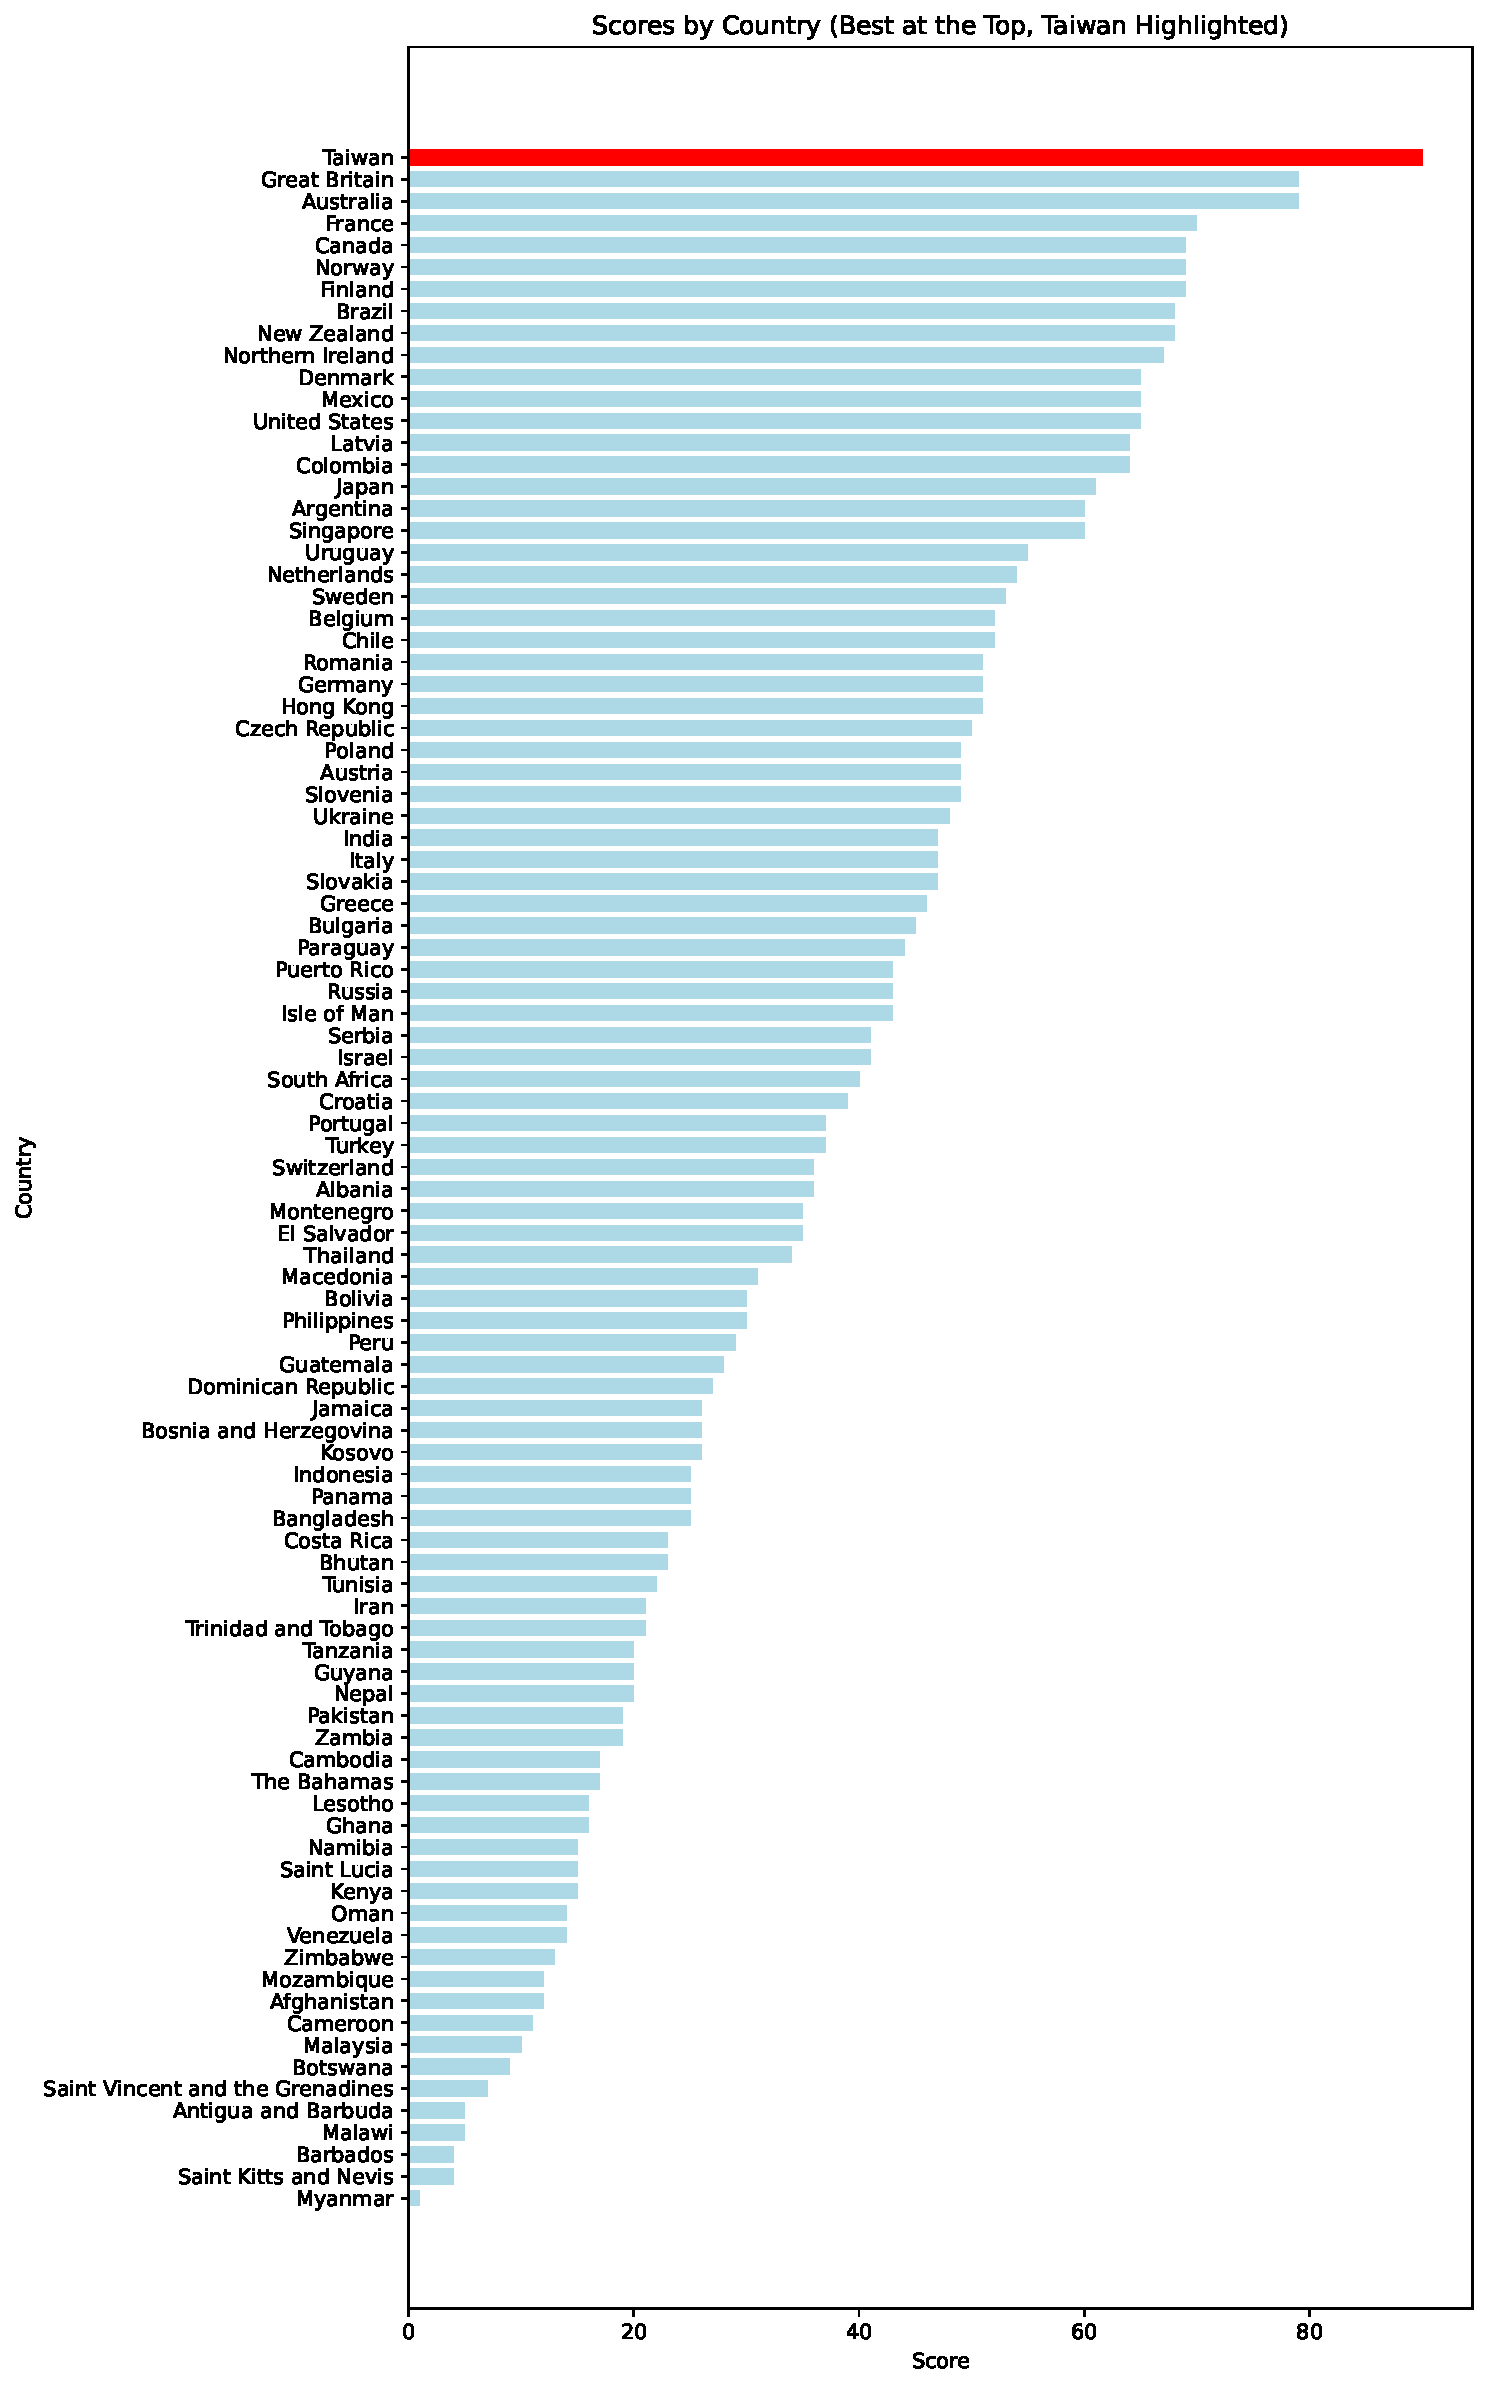
\includegraphics[keepaspectratio]{_thesis_files/figure-pdf/fig-open-data-index-output-1.pdf}}

}

\caption[Open Data Index]{\label{fig-open-data-index}Open Data Index}

\end{figure}%

Other indexes do not include Taiwan in the TOP 10.

\begin{figure}

\centering{

\pandocbounded{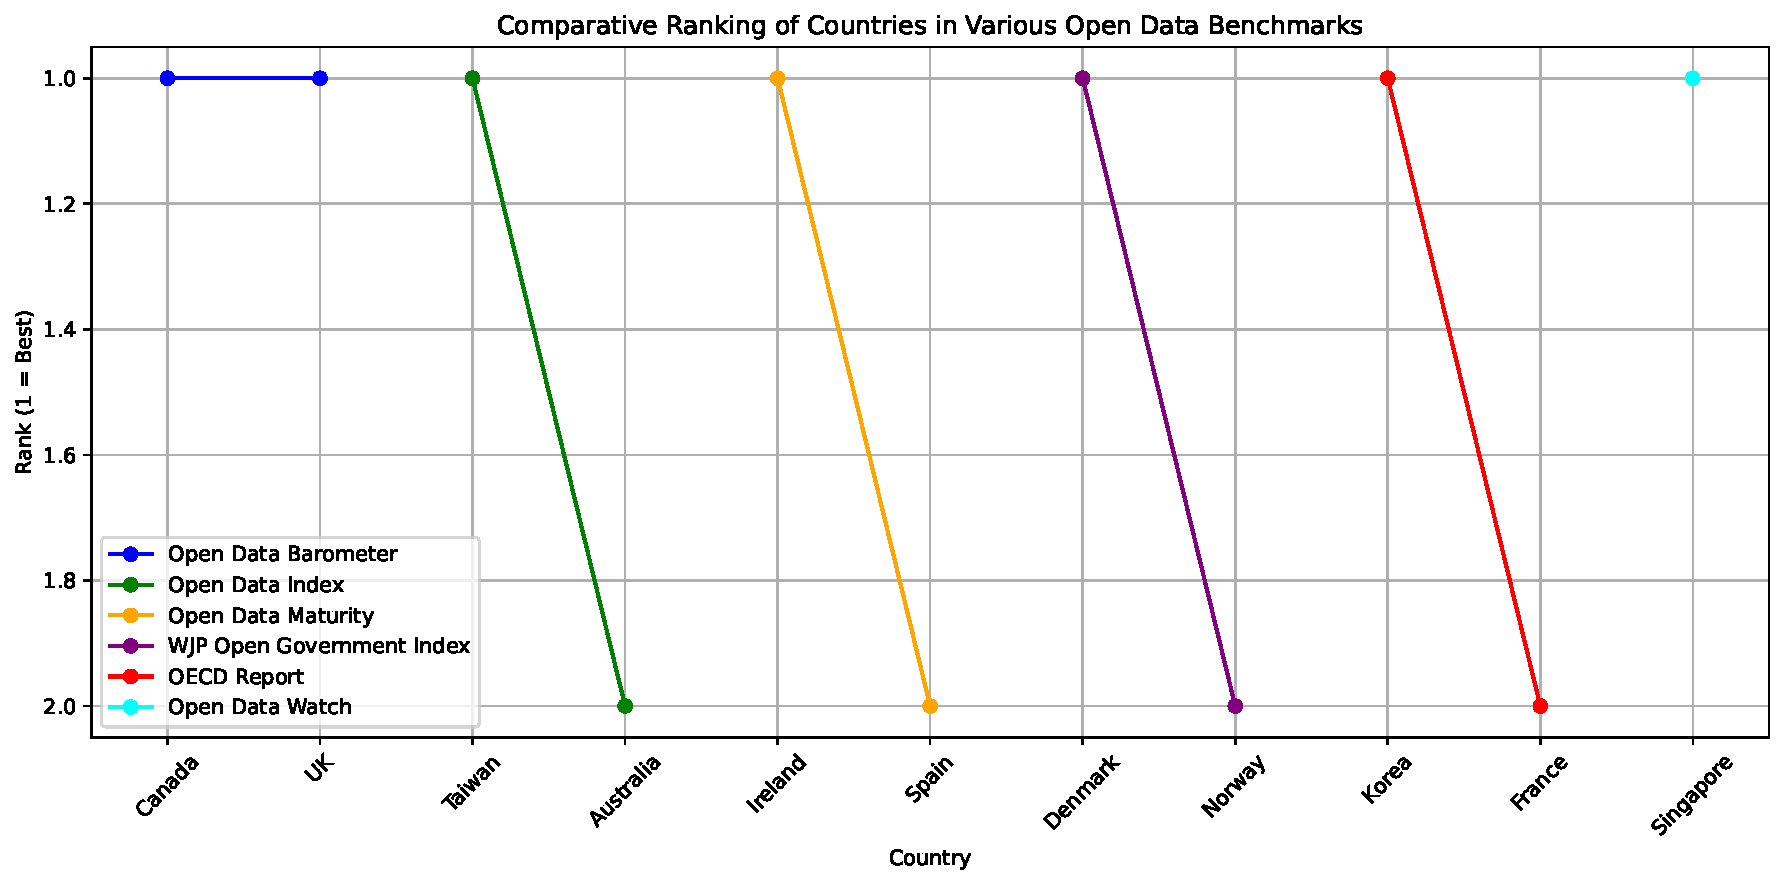
\includegraphics[keepaspectratio]{_thesis_files/figure-pdf/fig-open-data-compare-output-1.pdf}}

}

\caption[Alternative Open Data
Indexes]{\label{fig-open-data-compare}Alternative Open Data Indexes}

\end{figure}%

Data-driven design requires access to data, making the movement towards
\emph{open data sharing} very important. Some countries and cities are
better than others at sharing data openly.

\def\pandoctableshortcapt{Examples of Cities and Countries That Share
Data Openly}

\begin{longtable}[]{@{}ll@{}}
\caption[Examples of Cities and Countries That Share Data
Openly]{Examples of cities and countries that share data openly. Data
sourced from (Government of Malaysia, 2025; Monetary Authority of
Singapore, 2023; {``Sveriges Dataportal,''} 2025)}\tabularnewline
\toprule\noalign{}
Country & Project \\
\midrule\noalign{}
\endfirsthead
\toprule\noalign{}
Country & Project \\
\midrule\noalign{}
\endhead
\bottomrule\noalign{}
\endlastfoot
Sweden & Swedish open data portal \\
Malaysia & Malaysian open data portal \\
Singapore & Singapore ESG open data platform \\
\end{longtable}

\let\pandoctableshortcapt\relax

To give a concrete example of the usefulness of open data, for instance,
the Open Data Portal of Malaysia shows a steady decline in Permanent
Reserved Forests (PRF) for anyone interested, without having to submit
any letter of request or communicate with officials; the data is just
directly accessible and includes a permissive license (Malaysia, 2024).
Likewise, in Singapore, the Monetary Authority has launched an open data
portal for ESG information, allowing anyone to delve into environmental,
social, and governmental topics (Monetary Authority of Singapore, 2023).

\begin{figure}

\centering{

\pandocbounded{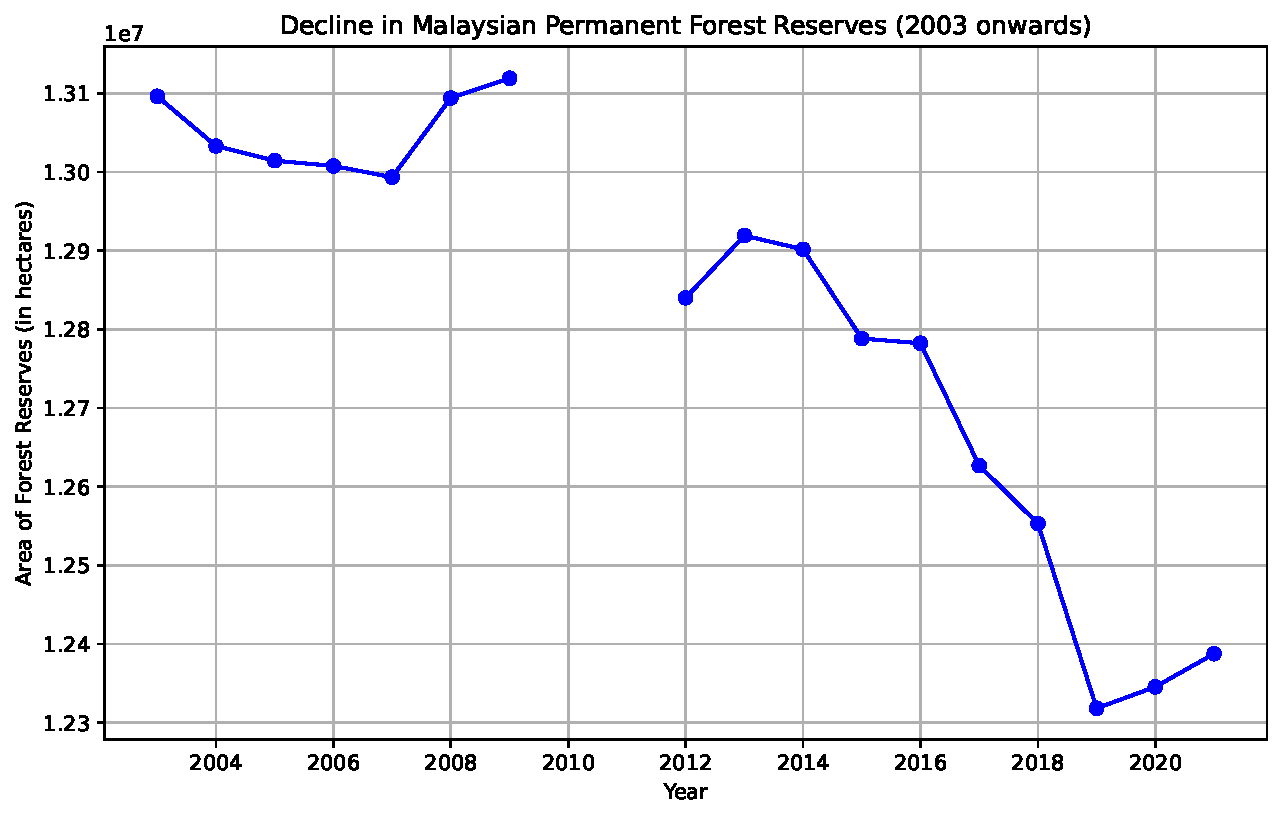
\includegraphics[keepaspectratio]{_thesis_files/figure-pdf/fig-mal-forests-output-1.pdf}}

}

\caption[Open Data As An Information Source for Environmental
Decline]{\label{fig-mal-forests}Open Data As An Information Source for
Environmental Decline}

\end{figure}%

\subsection{Context Design: Behavioral Nudges Towards Green Defaults in
Sustainable
Superapps}\label{context-design-behavioral-nudges-towards-green-defaults-in-sustainable-superapps}

For several decades, marketing researchers have been looking into how to
affect human behavior towards increasing purchase decisions in commerce,
both offline and online, which is why the literature on behavioral
design is massive. One of the key concepts is \emph{nudge}, first coined
in 2008 by the Nobel-winning economist Richard Thaler; nudges are based
on a scientific understanding of human psychology and shortcuts and
triggers that human brains use and leverages that knowledge to influence
humans in small but powerful ways (Thaler \& Sunstein, 2009).

The principles of nudge have also been applied to sustainability. For
example, a small study (n = 33) in the Future Consumer Lab in Copenhagen
by (Perez-Cueto, 2021) found that designing a ``dish-of-the-day'' which
was prominently displayed helped to increase vegetarian food choice by
85\%. Experiments by (Guath et al., 2022) focused on environmentally
friendly online purchases in Sweden (n = 200) suggest nudging can be
effective in influencing online shopping behavior towards more
sustainable options. A study of behavior change in Australia at large
university setting (N = 156) by (Novoradovskaya et al., 2021) found
nudging behavioral change had a significant effect and the author
suggested it may help to avoid some of the \emph{``16 billion paper
coffee cups are being thrown away every year''} globally (based on the
abstract - I was unable to access the full paper).

Google uses nudges in Google Flights and Google Maps, which allow
filtering flights and driving routes by the amount of
CO\textsubscript{2} emissions, as well as surfacing hotels with Green
Key and EarthCheck credentials, while promising new sustainability
features across its portfolio of products (Sundar Pichai, 2021). Such
tools are small user interface nudges which Google's research calls
\emph{digital decarbonization}, defined by (Implement Consulting Group,
2022) as \emph{``{[}m{]}aximising the enabling role of digital
technologies by accelerating already available digital solutions''}.

In (Kate Brandt \& Matt Brittin, 2022), Google's Chief Sustainability
Officer Kate Brandt set a target of ``at least 20-25\%''
CO\textsubscript{2} emission reductions in Europe to reach a net-zero
economy and the global announcement set a target of helping 1 billion
people make more sustainable choices around the world (Jeni Miles,
2022). In addition to end--users, Google offers digital decarbonization
software for developers, including the Google Cloud Carbon Footprint
tool and invests in regenerative agriculture projects (Google, 2023;
\emph{Inside {Google}'s Regenerative Agriculture Play {\textbar}
{Greenbiz}}, 2021). While Google has launched several climate-focused
initiatives, it missed its CO\textsubscript{2}eq reduction targets due
to growing need for AI models (Worthington, 2025a).

Google has launched eco--focused features across its range of products:
search improvements for finding hybrid and electric vehicles; green
routes for driving, in collaborating with local city governments
sourcing data from the traffic lights to provide AI‐powered
optimizations, which allows the map to suggest routes which would reduce
fuel use and idling, complete with charging‐station info; also, better
navigation for cyclists (showing scooter and bike‐share options)
({``{Google mostrar{á} por defecto la ruta m{á}s 'verde' en su GPS y
ordenar{á} los vuelos seg{ú}n su impacto ambiental},''} 2021;
Worthington, 2025a). (Sarah Perez, 2022) shows how Google added features
to Flights and Maps to filter more sustainable options. Yet, critics say
updating the CO\textsubscript{2}eq calculations' math means Google
started hiding emissions, which Google denies, pointing to higher
accuracy of the carbon emissions modeling instead ({``Google
'Airbrushes' Out Emissions from Flying, {BBC} Reveals,''} 2022).
Google's Nest Renew smart-home product helped people shift heating,
ventilation, and air conditioning (HVAC) to use to cleaner grid times
(with an optional subscription service to match home electricity with
renewable electricity credits); in shopping searches, Google provides
energy‐efficient appliance recommendations, helping users choose
lower‐impact products at the point of purchase (Google, 2021; Justine
Calma, Oct 6, 2021, 10:01 AM GMT+3).

\def\pandoctableshortcapt{Examples of CO\textsubscript{2} Visibility in
Google's Products}

\begin{longtable}[]{@{}
  >{\raggedright\arraybackslash}p{(\linewidth - 4\tabcolsep) * \real{0.3699}}
  >{\raggedright\arraybackslash}p{(\linewidth - 4\tabcolsep) * \real{0.2603}}
  >{\raggedright\arraybackslash}p{(\linewidth - 4\tabcolsep) * \real{0.3699}}@{}}
\caption[Examples of CO~2~ Visibility in Google's Products]{Examples of
CO\textsubscript{2} visibility in Google's products.}\tabularnewline
\toprule\noalign{}
\begin{minipage}[b]{\linewidth}\raggedright
Feature
\end{minipage} & \begin{minipage}[b]{\linewidth}\raggedright
Product
\end{minipage} & \begin{minipage}[b]{\linewidth}\raggedright
Nudge
\end{minipage} \\
\midrule\noalign{}
\endfirsthead
\toprule\noalign{}
\begin{minipage}[b]{\linewidth}\raggedright
Feature
\end{minipage} & \begin{minipage}[b]{\linewidth}\raggedright
Product
\end{minipage} & \begin{minipage}[b]{\linewidth}\raggedright
Nudge
\end{minipage} \\
\midrule\noalign{}
\endhead
\bottomrule\noalign{}
\endlastfoot
Google Maps AI suggests more eco-friendly driving routes (Mohit Moondra,
n.d.) & Google Maps & Show routes with lower CO\textsubscript{2}
emissions; reduce stopping by using data from traffic lights. \\
Google Flights suggests flights with lower CO\textsubscript{2} emissions
& Google Flights & Show flights with lower CO\textsubscript{2}
emissions \\
Wizzair Check carbon impact (\emph{Offset Your Flight with {WIZZ}},
n.d.) & WizzAir & Offset on Checkout \\
\end{longtable}

\let\pandoctableshortcapt\relax

\begin{figure}[H]

{\centering 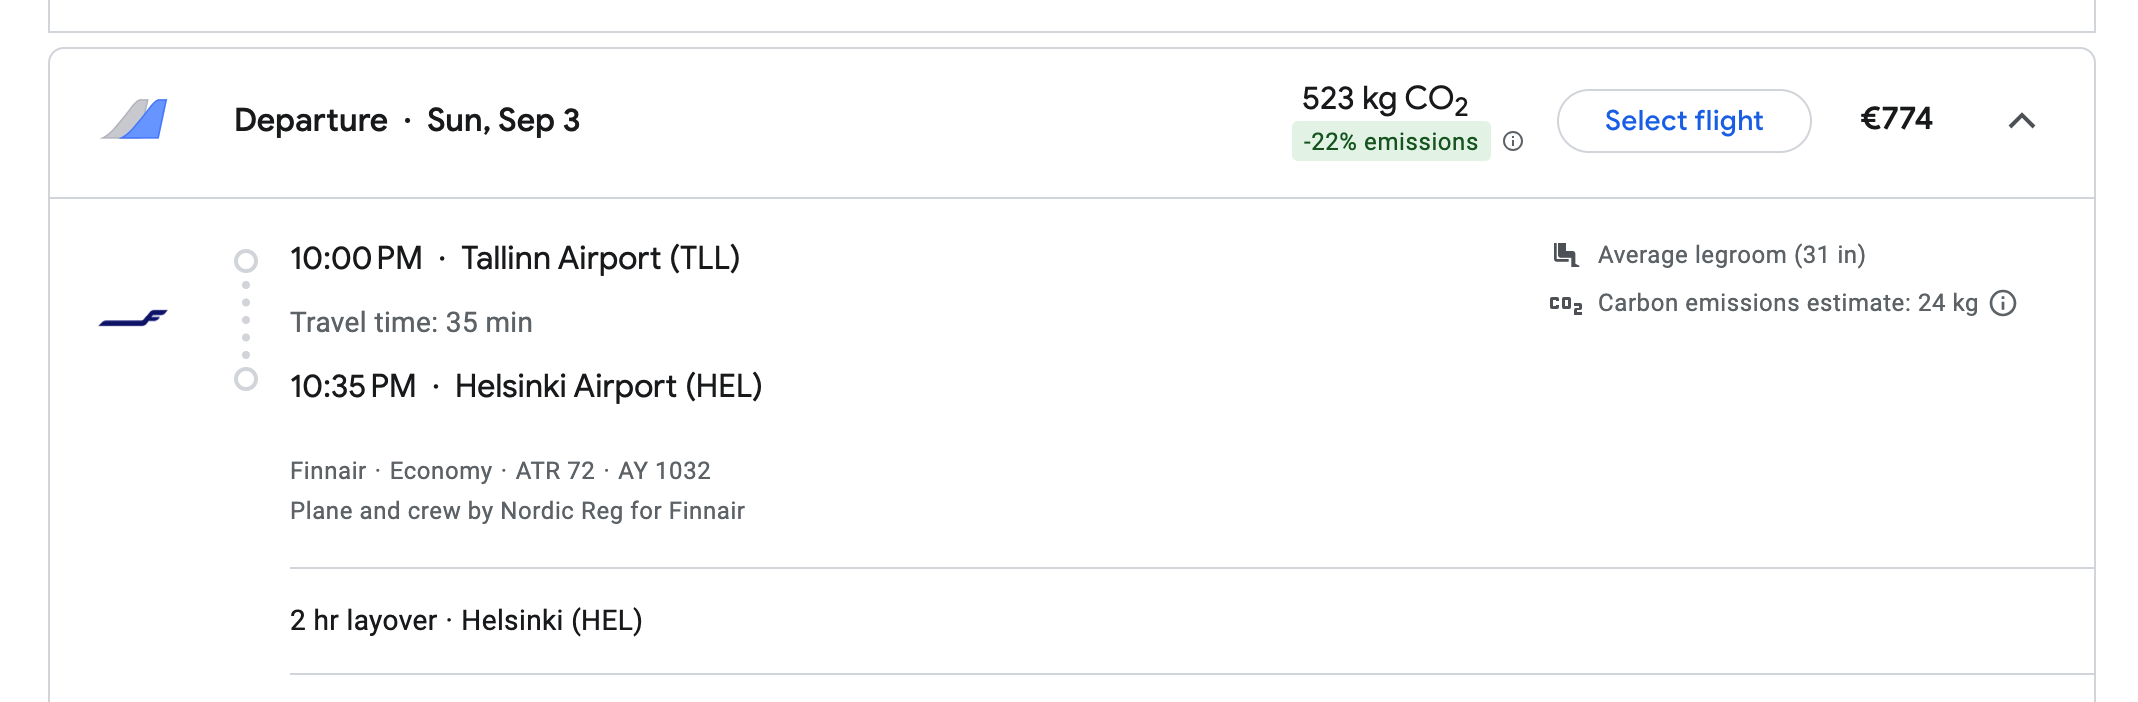
\includegraphics[width=1\linewidth,height=\textheight,keepaspectratio]{./images/design/flight-emissions.png}

}

\caption{Google's view of flight emissions}

\end{figure}%

(Wee et al., 2021) proposes 7 types of nudging technique based on an
overview of 37 papers which explore nudging people to be more
environmentally friendly.

\def\pandoctableshortcapt{Types of Nudge}

\begin{longtable}[]{@{}
  >{\raggedright\arraybackslash}p{(\linewidth - 2\tabcolsep) * \real{0.3611}}
  >{\raggedright\arraybackslash}p{(\linewidth - 2\tabcolsep) * \real{0.6389}}@{}}
\caption[Types of Nudge]{Types of nudge documented by (Wee et al.,
2021)}\tabularnewline
\toprule\noalign{}
\begin{minipage}[b]{\linewidth}\raggedright
Name
\end{minipage} & \begin{minipage}[b]{\linewidth}\raggedright
Technique
\end{minipage} \\
\midrule\noalign{}
\endfirsthead
\toprule\noalign{}
\begin{minipage}[b]{\linewidth}\raggedright
Name
\end{minipage} & \begin{minipage}[b]{\linewidth}\raggedright
Technique
\end{minipage} \\
\midrule\noalign{}
\endhead
\bottomrule\noalign{}
\endlastfoot
Prompting & Create cues and reminders to perform a certain behavior \\
Sizing & Decrease or increase the size of items or portions \\
Proximity & Change the physical (or temporal) distance of options \\
Presentation & Change the way items are displayed \\
Priming & Expose users to certain stimuli before decision-making \\
Labelling & Provide labels to influence choice (for example
CO\textsubscript{2} footprint labels) \\
Functional Design & Design the environment and choice architecture so
the desired behavior is more convenient \\
\end{longtable}

\let\pandoctableshortcapt\relax

(Acuti et al., 2023) makes the point that physical proximity to a
drop-off point helps people participate in sustainability and
metaphorical messaging alongside proximity can be powerful, enhancing
the ease of information processing. In a field study in Northern Italy,
a metaphor‐based message re-framed the factual statement ``1g of mercury
can pollute 1000L of water'' as ``7 bathtubs'', and 354000000L as ``140
Olympic swimming pools,'' (a projection of potential Italian mercury
pollution at current disposal rates), which significantly boosted
willingness to recycle mercury.

Alibaba's Ant Forest (螞蟻森林) has shown the potential gamified nature
protection, simultaneously raising money for planting forests and
building loyalty and brand recognition for their sustainable action,
leading the company to consider further avenues for gamification and
eco-friendliness.

\def\pandoctableshortcapt{Ant Forest Assisted Tree Planting - Growth
Story}

\begin{longtable}[]{@{}
  >{\raggedright\arraybackslash}p{(\linewidth - 6\tabcolsep) * \real{0.0857}}
  >{\raggedright\arraybackslash}p{(\linewidth - 6\tabcolsep) * \real{0.1857}}
  >{\raggedright\arraybackslash}p{(\linewidth - 6\tabcolsep) * \real{0.1857}}
  >{\raggedright\arraybackslash}p{(\linewidth - 6\tabcolsep) * \real{0.5429}}@{}}
\caption[Ant Forest Assisted Tree Planting - Growth Story]{Ant Forest
assisted tree planting; data compiled from (P. Cao \& Liu, 2023;
\emph{Over 600 {Million People Planted More Than} 326 {Million Trees}
via {Alipay Ant Forest} in {Five Years}}, 2021; UNFCCC, 2019; S. Wang et
al., 2022; X. Wang \& Yao, 2020; Z. Yang et al., 2018; B. Zhang et al.,
2022; F. Zhou et al., 2023; 张越熙, 2024; 李连环 \& 姜舒译, 2017; 胡群
\& 宋璠, 2024).}\tabularnewline
\toprule\noalign{}
\begin{minipage}[b]{\linewidth}\raggedright
Year
\end{minipage} & \begin{minipage}[b]{\linewidth}\raggedright
Users
\end{minipage} & \begin{minipage}[b]{\linewidth}\raggedright
Trees
\end{minipage} & \begin{minipage}[b]{\linewidth}\raggedright
Area
\end{minipage} \\
\midrule\noalign{}
\endfirsthead
\toprule\noalign{}
\begin{minipage}[b]{\linewidth}\raggedright
Year
\end{minipage} & \begin{minipage}[b]{\linewidth}\raggedright
Users
\end{minipage} & \begin{minipage}[b]{\linewidth}\raggedright
Trees
\end{minipage} & \begin{minipage}[b]{\linewidth}\raggedright
Area
\end{minipage} \\
\midrule\noalign{}
\endhead
\bottomrule\noalign{}
\endlastfoot
2016 & N/A & N/A & N/A \\
2017 & 230 million & 10 million & N/A \\
2018 & 350 million & 55 million & 6500 acres?? \\
2019 & 500 million & 100 million & 112,000 hectares / 66, 000
hectares? \\
2020 & 550 million & 200 million & 2,7 million acres? \\
2021 & 600 million & 326 million & N/A \\
2022 & 650 million & 400 million & 2 million hectares \\
2023 & 690 million & 475 million & N/A \\
2024 & N/A & 548 million & 3.87 million hectares \\
2025 & N/A & N/A & N/A \\
\end{longtable}

\let\pandoctableshortcapt\relax

\begin{figure}

\centering{

\pandocbounded{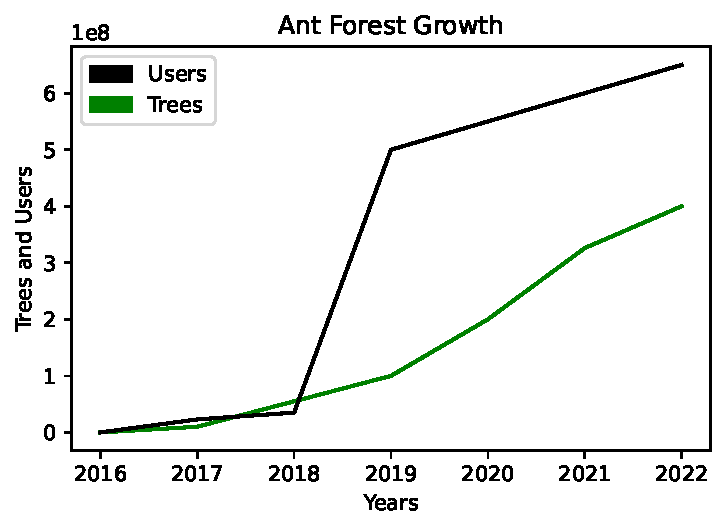
\includegraphics[keepaspectratio]{_thesis_files/figure-pdf/fig-ant-forest-growth-output-1.pdf}}

}

\caption[Growth of Ant Forest]{\label{fig-ant-forest-growth}Growth of
Ant Forest}

\end{figure}%

Ecosia is a search engine with an unconventional business models,
investing all its profits into planting trees, pouring €92 million into
climate action since 2009, planting 225 million trees worldwide (D. C.
Garcia, 2025b). The founder Christian Kroll recalls travelling in South
America in 2006 and being shocked to see vast areas of rainforests
converted into soy plantations, which inspired him to research the
causes of deforestation and start Ecosia; the company employs partners
around the world to improve soil, biodiversity, the water cycle,
reducing droughts and floods, and monitor the trees it plants (Hirsh,
2021).

New user interfaces hold some potential for sustainability improvements.
In particular, immersive communication technologies such as AR/VR hold
the potential to reduce business travel, if productive meetings can be
held online, reducing emissions. Likewise, visualizing large
architectural projects as well as simulating product design in various
industries can reduce cost by detecting problems in the 3D environment,
early on in the design process, especially for collaboration in teams
located all over the world (Varjo, 2025). Dynamic interfaces might
invoke a new, natural-interaction-focused design language, for taking
full advanced of extended reality (Hoang, 2022). First encouraging
findings from reconstructing language from fMRI readings (brain scans)
even show potential for enabling computers to directly read human minds;
contemporary AI models have already been shown capable of generating
full sentences from human thoughts (J. Tang et al., 2022).

The small screen estate space of mobiles phones and smart watches
necessitates displaying content in a dynamic manner. Likewise, speaking
is one mode of interaction that's become increasingly possible as
machines learn to interpret human language. Virtual reality glasses
(called AR/VR or XR in marketing speak) need dynamic content because the
user is able to move around the environment. All these are multi-modal
communication questions that interaction design is called upon to solve.

\def\pandoctableshortcapt{Modes of Interaction}

\begin{longtable}[]{@{}l@{}}
\caption[Modes of Interaction]{Modes of Interaction}\tabularnewline
\toprule\noalign{}
Modes of Interaction \\
\midrule\noalign{}
\endfirsthead
\toprule\noalign{}
Modes of Interaction \\
\midrule\noalign{}
\endhead
\bottomrule\noalign{}
\endlastfoot
Writing \\
Speaking \\
Touching \\
Moving \\
Seeing \\
\end{longtable}

\let\pandoctableshortcapt\relax

\subsection{Learning from Quantified Self: Tracking Health and
Lifestyle}\label{learning-from-quantified-self-tracking-health-and-lifestyle}

An early example of how tracking personal data enables behavior change,
are health and lifestyle tracking apps. Research on \emph{personal data
tracking} also known as \emph{quantified self} or \emph{self-monitoring}
is abundant. There's substantial academic evidence indicating that
health tracking apps can have a measurable impact on user health
behaviors and increase positive health outcomes. Wearable devices
including the Apple Watch, Oura Ring, Fitbit and others, combined with
apps, help users track a variety of health metrics. Recently, npj
Biosensing even published a device from the MIT Media Lab that can track
cells inside the human body from a wrist-worn device (Jang et al., 2025;
Jarvis, 2025).

Apart from health, wearable devices have been used to track other
metrics such as physiological parameters of students at school to
determine their learning efficiency (Giannakos et al., 2020). Not only
can health metrics be tracking, but exposure to pollution as well as
personal carbon footprint, are all to some extent track-able (if not
traceable).

\subsubsection{Health and Fitness
Tracking}\label{health-and-fitness-tracking}

Tracking one's health and fitness is a familiar mode of \emph{quantified
self}, available to many smartwatch users - and even pretty much to
anyone who has a phone made in the past decade. Apple is a leader in
health tracking, releasing Apple Health in 2008 as an iOS 8 software
feature and the Apple Watch in 2015, filled with health-focused sensors
and features (Apple, 2022b). In 2022 Apple outlined plans for
\emph{``empowering people to live a healthier day,''} promising a new
set of health-features with every release, such as the rumored
temperature measurement inside of Apple AirPod earphones; and providing
most of this data to developers through Apple's HealthKit health metrics
APIs, which app builders can tap into (Apple, 2022a, 2022c).

Use of wearable devices enables one to be more aware of one's health.
(Saubade et al., 2016) finds health tracking is useful for motivating
physical activity. Blood glucose tracking is popular even for people
without diabetes, to optimize their daily activity, including sports
({``Is Blood Sugar Monitoring Without Diabetes Worthwhile?''} 2021).
Smart toilets offer unobtrusive monitoring of urine for one's hydration
levels as well as deeper insights on biomarkers as well as renal and
nutritional health, through using sensor‐equipped seats (e.g.~Withings'
U-Scan), which create a daily stream of data useful for trend analysis
(Hermsen et al., 2023; Wagner \& Boiten, 2023). Companies like
NeuralLink are building devices to construct meaningful interactions
based only on brain waves (EEG) (Musk \& Neuralink, 2019).

Popular Strava sports assistant (over 100 million users) provides
activity tracking and feedback (Strava, 2022).

\begin{figure}[H]

{\centering 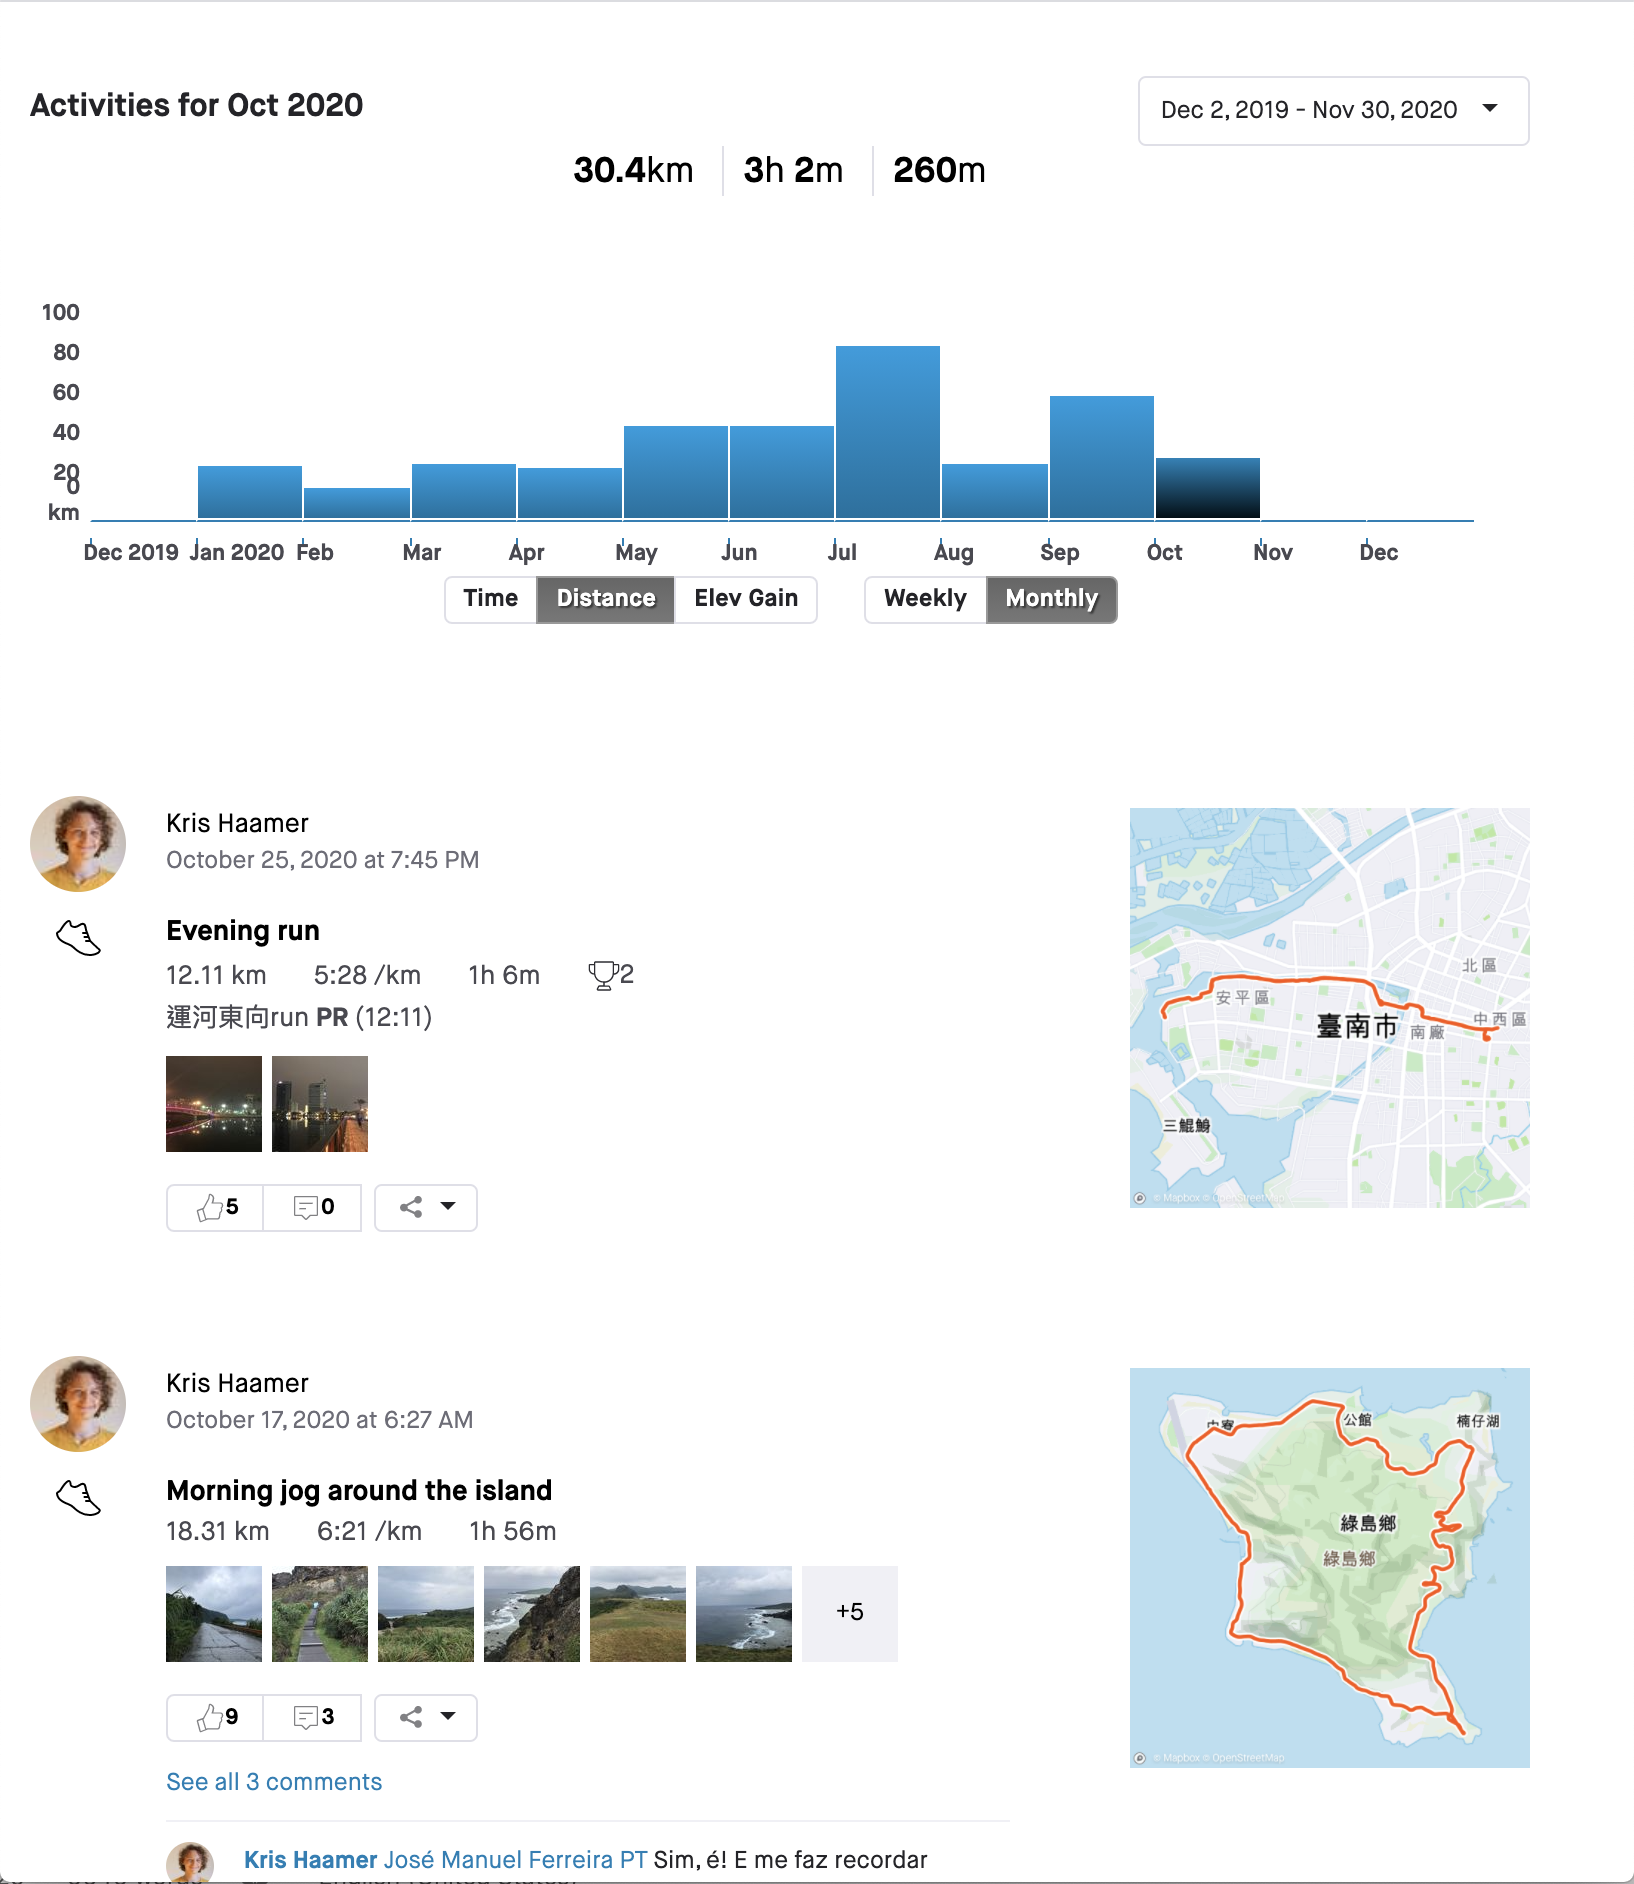
\includegraphics[width=1\linewidth,height=\textheight,keepaspectratio]{./images/design/strava.png}

}

\caption{Popular Strava sports assistant provides run tracking and
feedback}

\end{figure}%

Sleep quality is an important aspect of both physical and mental health
and many devices and apps focus on helping people get enough high
quality sleep. There's plenty of academic literature on how physical
activity, as well as environmental aspects, such as air quality, affect
sleep (X. Liu et al., 2019) tracks how wearable data is used for
tracking sleep improvements from exercise. (Grigsby-Toussaint et al.,
2017) made use of sleep apps to construct humans behaviors also known as
\emph{behavioral constructs}.

Being conscious of one's mental health improves quality of life. (Tyler
et al., 2022) surveyed the use of self-reflection apps in the UK (n =
998) finding a variety of methods from physical journaling in notebooks
to smartphone-based note-taking apps, reviewing printed photo albums,
and other digital tools.

Tracking one's food intake helps understanding how healthy and
nutrient-rich is one's diet. (Ryan, 2022) uses the ``capability
methodology'' framework, developed by economist Amartya Sen and later
expanded by philosopher Martha Nussbaum, shifting focus from what people
have (e.g.~money, food, tools) to what they are able to do (human
capabilities), which is used in the context of this paper to evaluate
not only if the apps provide healthy food suggestions, but to what
extent they expand a user's freedom to live a healthy life; some forms
of nudging inside the apps can support users' goals however manipulative
or coercive tactics serve only the app developers' interests and are
ethically problematic - the paper emphasizes the need for interaction
design that respect users' freedom, consider diverse personal choices,
diverse bodies, cultures, and preferences, and environmental factors.

The Oura ring is an example of \emph{calm technology}, providing helpful
data without calling an attention to itself (Phelan, 2024). More
recently, Oura Ring launched an AI-advisor to help explain the health
data recorded by its device: deliver contextual and personalized
guidance, remember past interactions while emphasizing privacy, and
analyze both short- and long-term biometric trends (Team, 2025). There's
value in developing standardized fitness metrics, which different
digital health providers can use to create dashboards with comparable
data. Even with messy data, AI has a useful role as a translator between
different standards. OpenAI is collaborating with ex-Apple designer Jony
Ive, to bring such ambient AI devices to live, which they believe has
the potential for a new product category (WSJ News, 2025).

\subsubsection{Pollution Exposure
Tracking}\label{pollution-exposure-tracking}

Pollution exposure tracking may be considered a combination of health
tracking and sustainability tracking. I've been tracking my personal air
pollution exposure using the Atmotube Pro device attached to my
backpack.

\begin{figure}

\centering{

\pandocbounded{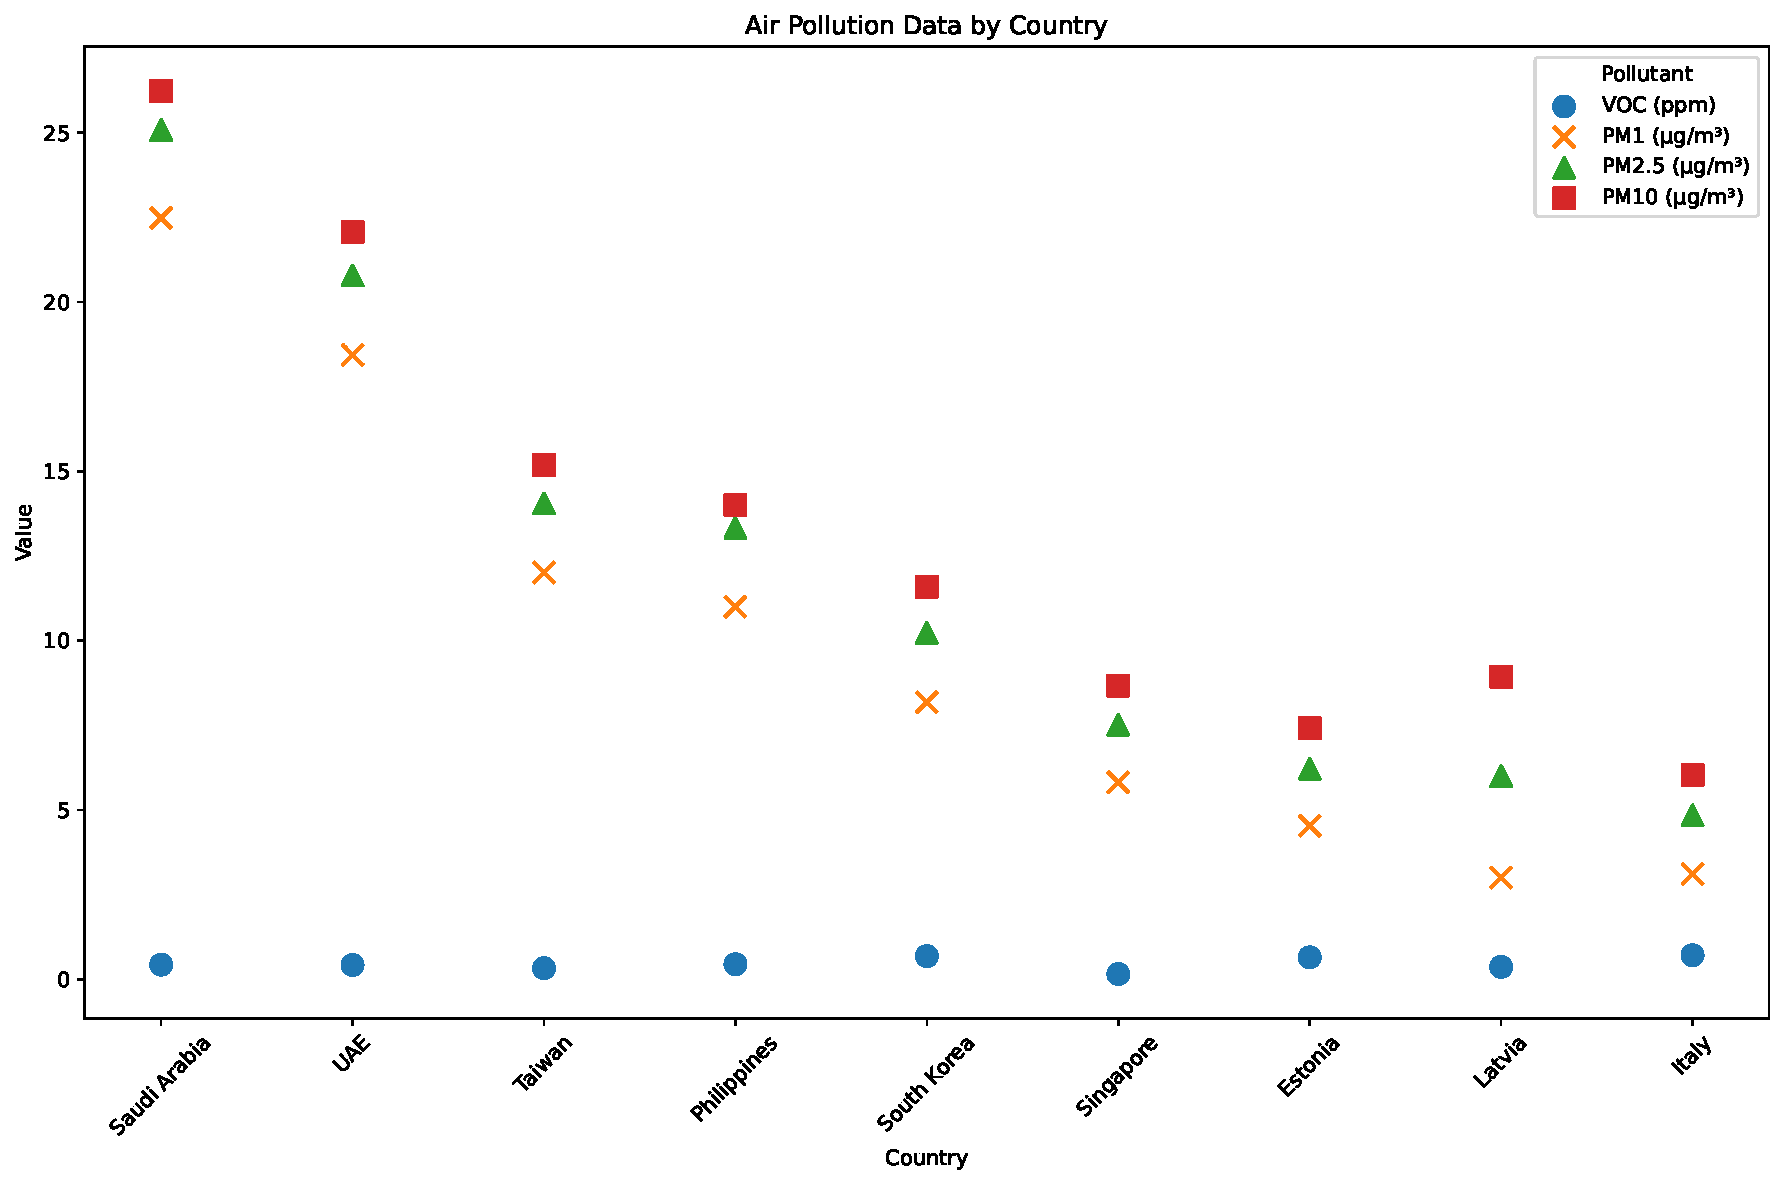
\includegraphics[keepaspectratio]{_thesis_files/figure-pdf/fig-air-pollution-personal-output-1.pdf}}

}

\caption[My Personal Exposure to Air
Pollution]{\label{fig-air-pollution-personal}My Personal Exposure to Air
Pollution}

\end{figure}%

The above chart shows my exposure to pollutants while traveling, ranked
from worst to best.

\subsubsection{Tracking Personal Sustainability and Carbon
Emissions}\label{tracking-personal-sustainability-and-carbon-emissions}

The above examples of tracking various aspects of health beg the
question if one could track personal sustainability in a similar
fashion. We have a limited carbon budget so calculating
CO\textsubscript{2}eq-cost could be expressly integrated into every
activity.

Already in 2017, a project funded by the EU Horizon 2020 title
\emph{``Instant Gratification for Collective Awareness and Sustainable
Consumerism''} piloted the concept of \emph{``political consumerism''},
by enabling shoppers at 2 stores (Estonia and Austria) to experience
real-time, personalized sustainability ratings on nearby products (by
using a mobile app and bluetooth beacons to locate shoppers at shelf
level, while maintaining privacy); instead of isolated choices,
individual preferences were (environmental, health, political)
aggregated into a community ``sustainability signal''; the results
indicated a statistically significant increase in sustainability
awareness and some users praised the simplicity of the user interface
(Bennati \& Pournaras, 2018; \emph{Instant {Gratification} for
{Collective Awareness} and {Sustainable Consumerism}}, 2022; Klinglmayr
et al., 2017; Pournaras et al., 2016).

More recently, (Kommenda et al., 2022) describes an interactive demo of
Carbon Food Labels in the Financial Times, aimed at influence purchasing
behavior by displaying Life Cycle Assessment (LCA) data directly on the
products; for example - lentils (1kg CO\textsubscript{2}eq per 1 kg)
v.s. beef (27kg CO\textsubscript{2}eq per 1 kg) - clearly illustrating
the contrasting climate impact of different foods; moreover, shoppers
could see the emissions in their shopping cart,enabling real-time
comparisons and decision-making; an accompanying survey showed 68\% of
users were interested in choosing lower-emission products while a low
22\% of the respondents trusted the data, highlighting a key challenge:
standardizing and verifying supply-chain data.

The founder of the Commons (formerly known as Joro) consumer
CO\textsubscript{2e} tracking app recounts how people have a gut feeling
about the 2000 calories one needs to eat daily, so perhaps daily
CO\textsubscript{2e} tracking could develop a gut feeling about one's
carbon footprint (Jason Jacobs, 2019). Zhang's Personal Carbon Economy
conceptualized the idea of carbon as a currency used for buying and
selling goods and services, as well as an individual carbon exchange to
trade one's carbon permits (S. Zhang, 2018). These type of app suggest
CO\textsubscript{2}eq calculations will be part of our everyday
experience. Nonetheless, sustaining user engagement over time in
sustainability tracking apps is challenging, because the perceived
personal benefit and measurable impact is so minimal - it may feel
meaningless.\hspace{0pt} Tracking sustainability may have collective
benefits but tracking health has immediate personal benefits. Health
apps feel tangible with increased well-being while sustainability apps
often feel more collective, long-term and sometimes with benefits too
small to matter, making it harder to motivate individual users.

Sustainability tracking, while perhaps less than health tracking, can
also have a measurable impact. One study of personal carbon footprint
tracking apps (aka CO\textsubscript{2}eq calculators) in a mid-sized
German city (n = 216) helped overall emission reduction by 23\%
correlating with feedback from the app specifically reducing emissions
from heating 26.9\%, food 16.4\%, household 34.7\% reduction, and
mobility 12\% (S. Hoffmann et al., 2024). Better maps can also convince
people to make changes; advanced maps which visualize erosion, heat,
flooding, fire, drought, extreme weather, and other climate risks, can
inform resilience planning; a map for transport, such as taxis, can
visualize pickup / drop-off imbalances, coloring areas green where
pickups exceed drop-offs and orange where drop-offs exceed pickups, can
help users see spatial patterns and inform climate-resilient transport
planning (Carto, 2023).

Because of the large emission footprint of transport, offering a steep
emissions reduction potential, greener modes of mobility have been
heavily researched. Already more than a decade ago, a survey from April
2014 to December 2015 (n = 4586, total 29930 travel episodes) across the
United Kingdom, asked participants to rate their enjoyment (on a liker
scale from 1 to 7) and tracked the type of travel (work, unpaid work,
personal care, childcare, leisure, etc); results showed private car was
used for 79\% of personal care and 55\% of leisure trips; key findings
showed \emph{walking and cycling significantly increase enjoyment}
across all trip purposes, while public transit reduced enjoyment for
childcare and work-related travel; overall findings show improvements in
transport infrastructure can both lower green house gas emissions and
boost traveler wellbeing (Echeverría et al., 2022).

A wide range of personal carbon footprint calculators have been released
online, ranging from those made by governments and companies to student
projects. Similar to personal health trackers, personal
CO\textsubscript{2} trackers help one track emissions and suggests
sustainable actions. In Singapore, the DBS bank released a consumer
sustainability ESG app called DBS LiveBetter (DBS, 2018; DBS Singapore,
n.d.)

\def\pandoctableshortcapt{A Selection of Personal Sustainability Apps}

\begin{longtable}[]{@{}
  >{\raggedright\arraybackslash}p{(\linewidth - 2\tabcolsep) * \real{0.3611}}
  >{\raggedright\arraybackslash}p{(\linewidth - 2\tabcolsep) * \real{0.6389}}@{}}
\caption[A Selection of Personal Sustainability Apps]{A selection of
personal sustainability apps.}\tabularnewline
\toprule\noalign{}
\begin{minipage}[b]{\linewidth}\raggedright
App
\end{minipage} & \begin{minipage}[b]{\linewidth}\raggedright
Description
\end{minipage} \\
\midrule\noalign{}
\endfirsthead
\toprule\noalign{}
\begin{minipage}[b]{\linewidth}\raggedright
App
\end{minipage} & \begin{minipage}[b]{\linewidth}\raggedright
Description
\end{minipage} \\
\midrule\noalign{}
\endhead
\bottomrule\noalign{}
\endlastfoot
Commons (Formerly Joro) & Finacial Sustainability Tracking + Sustainable
Actions \\
Klima & Offset Subscription \\
Wren & Offset Subscription \\
JouleBug & CO\textsubscript{2}eq tracking \\
eevie & \\
Aerial & \\
EcoCRED & \\
Carbn & \\
LiveGreen & \\
Earth Hero & \\
\end{longtable}

\let\pandoctableshortcapt\relax

(G. Shin et al., 2019)'s synthesis review of 463 studies shows wearable
devices have potential to influence behavior change towards healthier
lifestyles. While the behavior changes may sound simple - like switching
from driving to walking - and would have and effect both on health and
the environmental, they are hindered by factors from personal motivation
to (lack of) suitable urban architecture. (Delclòs-Alió et al., 2022)
discusses walking in Latin-American cities. Walking is the most
sustainable method or transport but requires the availability of city
infrastructure, such as sidewalks, which many cities still lack. The
urban environment has an influence on health. (Sanchez et al., 2022)
suggests tracking users using their smartphones and attributing points
for actions deemed beneficial - yet this has potential privacy issues.
For any service tracking the user's action, following privacy UX
guidelines is crucial (Jarovsky, 2022b).

\begin{figure}

\centering{

\pandocbounded{\includegraphics[keepaspectratio]{_thesis_files/figure-pdf/fig-bad-behav-output-1.pdf}}

}

\caption[Increase of Bad Behavior During the COVID19
Pandemic]{\label{fig-bad-behav}Increase of Bad Behavior During the
COVID19 Pandemic}

\end{figure}%

Human behavior is affected by the environment. The above chart shows the
incidence of bad behavior during the pandemic increased significantly in
Sweden based on data from (Ceccato et al., 2023).

\subsection{Digital Product Passports: Tracking Data for Sustainable
Product
Management}\label{digital-product-passports-tracking-data-for-sustainable-product-management}

\emph{Digital Product Passports}, part of the Sustainable Products
Initiative, are one of the key actions take under the Circular Economy
Action Plan (CEAP) of the European Union; the goal of this initiative is
to lay the groundwork for a gradual introduction of a digital product
passports in at least 3 key markets by 2024: (1) batteries for electric
vehicles and industrial use, (2) consumer and ICT electronics, (3)
textiles and apparel (Kuch, 2022). (Nissinen et al., 2022) calls for
emissions data to be made available to manufacturers, retailers, and
consumers so they can make low-carbon choices; moreover, metrics must
move beyond a single aggregated number to assessing life-cycle
emissions' variability.

In theory, DPPs are able to capture and make usable the comprehensive
trace of data needed for green transformation. Even though \emph{digital
product passports} relate heavily to adopting a circular economy, I've
chosen to highlight this topic under Design, as it's the main design
implication from this chapter - an emerging technology which needs to be
\emph{designed}.(King et al., 2023) proposes a universal definition of a
Digital Product Passport Ecosystem (DPPE) as a ``system-of-systems,''
synthesizing stakeholder requirements and concerns from the EU's open
consultation on the Sustainable Products Initiative, aiming to influence
consumer behavior towards sustainable purchasing - and responsible
product ownership - by making the sustainability aspects of a product
life cycle clearly apparent. (Reich et al., 2023) identifies
\emph{information gaps} as one of the major obstacles to realizing a
circular economy; a study of 28 experts across academia, industry,
government, consultancy and NGOs, showed Digital Product Passports
(DPPs) can enhance the 9 ``R'' in circular strategies. The first full
articulation of the 9 R strategies came from the report \emph{``Circular
Economy -- Measuring Innovation in the Product Chain''}, where (Potting
et al., 2017) laid out a hierarchy of circular‐economy options; the
framework was later adopted and popularized in peer-reviewed literature,
for example (Kirchherr et al., 2017).

\def\pandoctableshortcapt{The R Strategies}

\begin{longtable}[]{@{}
  >{\raggedright\arraybackslash}p{(\linewidth - 2\tabcolsep) * \real{0.3056}}
  >{\raggedright\arraybackslash}p{(\linewidth - 2\tabcolsep) * \real{0.6944}}@{}}
\caption[The R Strategies]{The 9 R strategies from (Potting et al.,
2017).}\tabularnewline
\toprule\noalign{}
\begin{minipage}[b]{\linewidth}\raggedright
R-Strategy
\end{minipage} & \begin{minipage}[b]{\linewidth}\raggedright
Definition
\end{minipage} \\
\midrule\noalign{}
\endfirsthead
\toprule\noalign{}
\begin{minipage}[b]{\linewidth}\raggedright
R-Strategy
\end{minipage} & \begin{minipage}[b]{\linewidth}\raggedright
Definition
\end{minipage} \\
\midrule\noalign{}
\endhead
\bottomrule\noalign{}
\endlastfoot
R9 Recover & Incineration of material (energy recovery) \\
R8 Recycle & Process materials, obtaining the same (high grade) or lower
grade quality \\
R7 Repurpose & Use discarded product (or its parts) in a new product
(with a different function) \\
R6 Remanufacture & Use parts of a discarded product in a new product
(with the same function) \\
R5 Refurbish & Restore an old product (bring it up to date) \\
R4 Repair & Maintenance of a product so it can be used with its original
function \\
R3 Reuse & Reuse by another consumer (still in good condition and
fulfills its original function) \\
R2 Reduce & Increase efficiency in product manufacture (consume fewer
natural resources and materials) \\
R1 Rethink & Use the product more intensively (sharing the product via
online platforms, etc) \\
R0 Refuse & Don't use product at all (or replace the function with a
better alternative) \\
\end{longtable}

\let\pandoctableshortcapt\relax

There's extensive literature on the use Digital Product Passports (DPP)
at specific industries and for particular use cases, often focused on
improved efficiencies. (Plociennik et al., 2022) details the use of
Digital Product Passports and the cloud platform infrastructure to
improve e-waste sorting when paired with ML-based object detection.
(Berger, Rusch, et al., 2023) outlines data-science and machine-learning
approaches (for example sharing models) to enable the exchange of
sensitive EV-battery life-cycle data through Digital Product Passports,
while preserving confidentiality, helping overcome stakeholder
reluctance. (Jensen et al., 2023) study of mechatronics supply chains
found DPPs \emph{``support decision-making throughout product life
cycles in favor of a circular economy''}; specifically:

\begin{quote}
\begin{enumerate}
\def\labelenumi{(\arabic{enumi})}
\tightlist
\item
  usage and maintenance
\item
  identification
\item
  materials
\item
  guidelines
\item
  supply-chain and reverse logistics
\item
  environmental data
\item
  compliance
\end{enumerate}
\end{quote}

With the increasing electrification of transport, finding ways to deal
with the batteries is a crucial area of research. (Berger, Baumgartner,
Weinzerl, Bachler, Preston, et al., 2023) examined the stakeholders of
electric vehicle (EV) battery value-chain and mapped their data
requirements and current availability, laying groundwork to propose a
\emph{Digital Battery Passport}.(Berger, Baumgartner, Weinzerl, Bachler,
\& Schöggl, 2023) lists current challenges with EV batteries, providing
empirical insights into difficulties with DPP adoption, including
technical, organizational, and policy barriers; an interesting part of
the research is the introduction go \emph{``Sustainable Product
Management''} (SPM) as a specific field of management in the context of
circular economy.

They key barriers to adoption from (Berger, Baumgartner, Weinzerl,
Bachler, \& Schöggl, 2023) include:

\begin{quote}
Uncertainty of stakeholders Technological barriers Insufficient
willingness to share information Lack of clear legal requirements and
standards
\end{quote}

Meanwhile the enablers include:

\begin{quote}
Clear legal requirements Relative advantages (reputation gains, access
to new markets access, risk avoidance, marketing) Monetary incentives
(such as payments for data) Intrinsic motivation (compatibility with the
values)
\end{quote}

Focusing on food production industries, a brief historical overview of
previous efforts in this area may be helpful, to contextualize the
discussion. CO\textsubscript{2e} labeling initiatives represent an early
attempt to communicate the environmental cost of each product. Using
carbon labels to convey CO\textsubscript{2e} emission of consumer
products has been a topic of discussion for decades (Adam Corner, 2012).
Academic literature has looked at minute details such as color and
positioning of the label (S. Zhou et al., 2019). There's some indication
consumers are willing to pay a small premium for
low-CO\textsubscript{2e} products; all else being equal, consumers
choose the option with a lower CO\textsubscript{2e} number (Carlsson et
al., 2022; M. Xu \& Lin, 2022). (Cohen \& Vandenbergh, 2012) argues
labeling the carbon footprint of products does help inform consumer
choice towards sustainability and help promote a green economy. A
large-scale study of UK university students finds some evidence to
suggest labeling low CO\textsubscript{2e} food enables people to choose
a \emph{climatarian diet}, however the impact of carbon labels on the
market share of low-carbon meals is negligible (Lohmann et al., 2022).

Similar to to \emph{Nutritional Facts Labeling}, \emph{Carbon Labels}
provide basic information regarding the emissions' profile of each
product, yet taken alone, without a systemic push for carbon reduction,
they are insufficient to drive significant behavioral change. A study in
Sweden underlines a negative correlation between worrying about climate
impact and interest in climate information on products (Edenbrandt \&
Lagerkvist, 2022). This latter finding may be interpreted to suggest a
need for wider environmental education programs among consumers. (Asioli
et al., 2022) found differences between countries, where Spanish and
British consumers chose meat products with \emph{`no antibiotics ever'}
over a \emph{Carbon Trust} label, whereas French consumers chose
CO\textsubscript{2} labeled meat products. Despite ongoing interest,
several studies have shown that the overall impact of carbon labeling on
consumer behavior remains negligible. The idea is yet to find mainstream
adoption and participation in carbon labeling schemes remains voluntary,
with only a limited number of companies implementing such practices,
although their numbers are gradually increasing. Notable examples
include the U.S.-based restaurant chain \emph{Just Salad} , U.K.-based
vegan meat-alternative \emph{Quorn}, and plant milk \emph{Oatly}, all of
which provide carbon labeling on their products (Brian Kateman, 2020).
(ClimatePartner, 2020) Companies like ClimatePartner and Carbon Calories
offers labeling consumer goods with emission data as a service. (The
Carbon Trust, n.d.) The Carbon Trust reports it's certified 270000
product emissions' footprints.

\def\pandoctableshortcapt{Companies With Carbon Labels}

\begin{longtable}[]{@{}ll@{}}
\caption[Companies With Carbon Labels]{Companies with Carbon Labels
(Brian Kateman, 2020)}\tabularnewline
\toprule\noalign{}
Company & Country \\
\midrule\noalign{}
\endfirsthead
\toprule\noalign{}
Company & Country \\
\midrule\noalign{}
\endhead
\bottomrule\noalign{}
\endlastfoot
Just Salad & U.S.A. \\
Quorn & U.K. \\
Oatly & U.K. \\
IKEA & Sweden \\
\end{longtable}

\let\pandoctableshortcapt\relax

\def\pandoctableshortcapt{Organizations Who Certify Carbon Labels}

\begin{longtable}[]{@{}ll@{}}
\caption[Organizations Who Certify Carbon Labels]{Organizations Who
Certify Carbon Labels (ClimatePartner, 2020).}\tabularnewline
\toprule\noalign{}
Organization & Number of Certified Products \\
\midrule\noalign{}
\endfirsthead
\toprule\noalign{}
Organization & Number of Certified Products \\
\midrule\noalign{}
\endhead
\bottomrule\noalign{}
\endlastfoot
ClimatePartner & \\
Carbon Calories & \\
Carbon Trust & 27000 \\
\end{longtable}

\let\pandoctableshortcapt\relax

Transitioning from simpler carbon labels to data-driven \emph{Digital
Product Passports} requires comprehensive data collection on product's
history, composition, and environmental impact, digital infrastructure,
industry collaboration, regulatory frameworks, and consumer engagement.

\def\pandoctableshortcapt{Digital Product Passport Goals}

\begin{longtable}[]{@{}l@{}}
\caption[Digital Product Passport Goals]{Digital Product Passport goals
(Stretton, 2022a).}\tabularnewline
\toprule\noalign{}
Goal \\
\midrule\noalign{}
\endfirsthead
\toprule\noalign{}
Goal \\
\midrule\noalign{}
\endhead
\bottomrule\noalign{}
\endlastfoot
Sustainable Product Production \\
Businesses to create value through Circular Business Models \\
Consumers to make more informed purchasing decisions \\
Verify compliance with legal obligations \\
\end{longtable}

\let\pandoctableshortcapt\relax

(Van Capelleveen et al., 2023) conducted a comprehensive, structured
review of 200 academic papers on Digital Product Passports and related
concepts, including circular, product, material, resource, recycling,
and cradle-to-cradle variants, assessing dimensions such as historical
developments, stakeholders, goals, challenges, and designs for
solutions, in order to formalize the concept and its boundaries, finally
synthesizing a unified definition:

\begin{quote}
\emph{``a digital interface composing a certified identity of a single
identifiable product by accessing the set of life cycle registrations
linked to this object in order to yield insight into the sustainability
and circularity characteristics, the circular value estimation, and the
circular opportunities for both that product and its underlying
components and materials.''}
\end{quote}

Circularise, a leader in providing digital product passports as a
service, lists 15 types of data that should be include in a DPP (Tian
Daphne \& Chris Stretton, 2023). A case study of rigid polyurethane foam
(PU foam), a lightweight insulation material, explains how Circularise
used blockchain and zero-knowledge proof (ZKP) to allow for DPP
data-sharing, while retaining privacy and control over the data (Daphne,
2022; León, 2025).

\begin{figure}

\centering{

\pandocbounded{\includegraphics[keepaspectratio]{_thesis_files/figure-pdf/fig-digit-prod-pass-output-1.pdf}}

}

\caption[Digital Product Passport Data
Categories]{\label{fig-digit-prod-pass}Digital Product Passport Data
Categories}

\end{figure}%

The above chart shows data categories used in Digital Product Passports
(DPPs) as defined by Circularise.

(Gnanasambandam et al., 2022) describes responsible product management
as embedding privacy, sustainability, and inclusion into product design
as core priorities, not afterthoughts. (Korzhova, 2020) works as a
\emph{Sustainable Product Manager} at Grover, an online platform which
offers product for rent; she details how rentals-based business model
has saved 360 tons of devices from going to waste (the author compares
the amount to about 15 truckloads of devices), which sums up to 4275
tons of CO\textsubscript{2} savings.

\newpage

\section{AI}\label{ai}

\begin{figure}[H]

{\centering \pandocbounded{\includegraphics[keepaspectratio]{./images/ai/abstract-ai.png}}

}

\caption{Visual abstract for the AI chapter}

\end{figure}%

\subsection{Human Patterns}\label{human-patterns}

The fact that AI systems work so well is proof that we live in a
measurable world. The world is filled with structures: nature, cultures,
languages, human interactions - all form intricate patterns. Computer
systems are increasingly capable in their ability copy these patterns
into computer models - known as machine learning. As of 2023, 97
zettabytes (and growing) of data was created in the world per year
(Soundarya Jayaraman, 2023). Big data is a basic requirement for
training AIs, enabling learning from the structures of the world with
increasing accuracy. Large data-sets such as the LAION-5B of 5.85
billion image-text pairs, were foundational for training AI to recognize
images (Romain Beaumont, 2022; Schuhmann et al., 2022). Just 3 years
later, \emph{generating} images with GenAI models is now fast enought to
create images in real-time while the user is typing (Dwarkesh Patel,
2024). Similarly huge data-sets exist about other types of media - and
the open Internet itself, albeit less structured, is a data-source
frequently scraped by AI-model builders. Representations of the real
world in digital models enable humans to ask questions about the
real-world structures and to manipulate them to create synthetic
experiments that may match the real world (if the model is accurate
enough). This can be used for generating human-sounding language and
realistic images, finding mechanisms for novel medicines as well as
understanding the fundamental functioning of life on its deep physical
and chemical level (No Priors: AI, Machine Learning, Tech, \& Startups,
2023). Venture capitalists backing OpenAI describe AI as a foundational
technology, which will unlock human potential across all fields of human
activity (Greylock, 2022).

In essence, \emph{human patterns} enable AIs. Already 90 years ago
(McCulloch \& Pitts, 1943) proposed the first mathematical model of a
neural network inspired by the human brain. Alan Turing's Test for
Machine Intelligence followed in 1950. Turing's initial idea was to
design a game of imitation to test human-computer interaction using text
messages between a human and 2 other participants, one of which was a
human, and the other - a computer. The question was, if the human was
simultaneously speaking to another human and a machine, could the
messages from the machine be clearly distinguished or would they
resemble a human being so much, that the person asking questions would
be deceived, unable to realize which one is the human and which one is
the machine? (Turing, 1950).

\begin{quote}
Alan Turing: \emph{``I believe that in about fifty years' time it will
be possible to program computers, with a storage capacity of about
10\textsuperscript{9}, to make them play the imitation game so well that
an average interrogator will not have more than 70 percent chance of
making the right identification after five minutes of questioning.
\ldots{} I believe that at the end of the century the use of words and
general educated opinion will have altered so much that one will be able
to speak of machines thinking without expecting to be contradicted.''} -
from (Stanford Encyclopedia of Philosophy, 2021)
\end{quote}

By the 2010s AI models became capable enough to beat humans in games of
Go and Chess, yet they did not yet pass the Turing test. AI use was
limited to specific tasks. While over the years, the field of AI had
seen a long process of incremental improvements, developing increasingly
advanced models of decision-making, it took an \textbf{\emph{increase in
computing power}} and an approach called \textbf{\emph{deep learning}},
a variation of \textbf{\emph{machine learning (1980s),}} largely modeled
after the \textbf{\emph{neural networks}} of the biological (human)
brain, returning to the idea of \textbf{\emph{biomimicry}}, inspired by
nature, building a machine to resemble the connections between neurons,
but digitally, on layers much deeper than attempted before. Like quantum
computing, AI more of a discovery, thank an invention; we have no idea,
what are the limits of intelligence (CatGPT, 2025).

Founder of NVIDIA, Jensen Huang, whose computer chips power much of this
revolution, calls it the \emph{``Intelligence Infrastructure''},
produced by intelligence factories, and integrated into everything, just
like electricity was (NVIDIA, 2025). In order to produce this
intelligence, huge AI factories are being built around the world,
measured in the energy requirements. (Calma, 2025) predicts AI will
surpass Bitcoin's energy use by the end of 2025 (Calma, 2025). The 500B
USD Stargate project, is currently building 1.2 gigawatts of AI capacity
in the Texas, and expanding to other areas around the U.S., and data
center in Abu Dhabi, U.A.E., which requires 5GW of energy, and is
physically bigger than the country of Monaco (Loizos, 2025; Moss, 2025).
In comparison, the 500MW xAI AI factory, built by Elon Musk's company,
powered by natural gas generators, is moderate in size (B. Wang, 2025).
While OpenAIs Sam Altman is repeatedly quoted as saying the productivity
gains created by AI will far offset any of its environmental footprint
or other words to that effect (Altman, 2024; Di Pizio, 2023), critics
like (iGenius, 2020) argue that AI cannot enable a sustainable future if
it is not sustainable by design; training and delivery of AI products
must include sustainability considerations tied into data intelligence
and business analytics.

\subsubsection{Human Feedback}\label{human-feedback}

Combining deep learning and \emph{reinforcement learning with human
feedback (RLHF)} enabled to achieve levels of intelligence high enough
to beat the Turing test (Christiano et al., 2017; Christiano, 2021; Kara
Manke, 2022). John Schulman, a co-founder of OpenAI describes RLHF
simply: \emph{``the models are just trained to produce a single message
that gets high approval from a human reader''} (Kara Manke, 2022).
Bigger models aren't necessarily better; rather models need human
feedback to improve the quality of responses (Ouyang et al., 2022).

The nature-inspired approach was successful. Innovations such as
\emph{back-propagation} for reducing errors through updating model
weights and \emph{transformers} for tracking relationships in sequential
data (for example in sentences), enabled AI models to became
increasingly capable (Merritt, 2022; Vaswani et al., 2017).
\textbf{\emph{Generative Adversarial Networks}} trained models through
pitting them against each other (Goodfellow et al., 2014).
\textbf{\emph{Large Language Models}}, enabled increasingly generalized
models, capable of more complex tasks, such as language generation
(Radford et al., 2018).

One of the leading scientists in this field of research, Geoffrey
Hinton, had attempted back-propagation already in the 1980s and
reminiscents how:

\begin{quote}
\emph{``the only reason neural networks didn't work in the 1980s was
because we didn't have have enough data and we didn't have enough
computing power''} (CBS Mornings, 2023).
\end{quote}

(Epoch AI, 2024) reports the growth in computing power and the evolution
of more than 800 AI models since the 1950s. Very simply, more data and
more computing power means more intelligent models.

\pandocbounded{\includegraphics[keepaspectratio]{_thesis_files/figure-pdf/cell-42-output-1.pdf}}

The above chart shows an illustration of how transformers work by
(Alammar, 2018).

By the 2020s, AI-based models became a mainstay in medical research,
drug development, patient care (Holzinger et al., 2023; Leite et al.,
2021), quickly finding potential vaccine candidates during the COVID19
pandemic (Zafar \& Ahamed, 2022), self-driving vehicles, including cars,
delivery robots, drones in the sea and air, as well as AI-based
assistants. The existence of AI models has wide implications for all
human activities from personal to professional. The founder of the
largest chimp-maker NVIDIA calls upon all countries do develop their own
AI-models which would encode their local knowledge, culture, and
language to make sure these are accurately captured (World Governments
Summit, 2024).

OpenAI has researched a wide range of approaches towards artificial
general intelligence (AGI), work which has led to advances in large
language models(AI Frontiers, 2018; Ilya Sutskever, 2018). In 2020
OpenAI released a LLM called GPT-3 trained on 570 GB of text (Alex
Tamkin \& Deep Ganguli, 2021) which was adept in text-generation.
(Singer et al., 2022) describes how collecting billions of images with
descriptive data (for example the descriptive \emph{alt} text which
accompanies images on websites) enabled researchers to train AI models
such as \textbf{\emph{stable diffusion}} for image-generation based on
human-language. These training make use of \emph{Deep Learning}, a
layered approach to AI training, where increasing depth of the computer
model captures minute details of the world. Much is still to be
understood about how deep learning works; even for specialists, the
fractal structure of deep learning can only be called \emph{mysterious}
(Sohl-Dickstein, 2024).

AI responses are probabilistic and need some function for ranking
response quality. Achieving higher percentage or correct responses
requires oversight which can come in the form of human feedback or by
using other AIs systems which are deemed to be already well-aligned
(termed Constitutional AI by Anthropic) (Bai et al., 2022; J. Bailey,
2023). One approach to reduce non-alignmnet issues with AI is to
introduce some function for human feedback and oversight to automated
systems. Human involvement can take the form of interventions from the
AI-developer themselves as well as from the end-users of the AI system.
Such feedback is not only provided by humans, computer can give feedback
to computers too. Less powerful AIs are taught by more poweful and
aligned AIs, which understand the world better, to follow human values:
for example META used LLAMA 2 for aligning LLAMA 3.

There are many examples of combination of AI and human, also known as
\emph{``human-in-the-loop'',} used for fields as diverse as training
computer vision algorithms for self-driving cars and detection of
disinformation in social media posts (Bonet-Jover et al., 2023; Jingda
Wu et al., 2023). Also known as Human-based computation or Human-aided
Artificial Intelligence (Mühlhoff, 2019; Shahaf \& Amir, 2007). (Ge
Wang, 2019) from the Stanford Institute for Human-Centered Artificial
Intelligence, describes core design principles for building interactive
AI systems that augment rather than replace people: (1) value human
agency, (2) offer granularity of control, and (3) provide transparency
interfaces.

\def\pandoctableshortcapt{Human-in-the-Loop Apps}

\begin{longtable}[]{@{}
  >{\raggedright\arraybackslash}p{(\linewidth - 4\tabcolsep) * \real{0.2639}}
  >{\raggedright\arraybackslash}p{(\linewidth - 4\tabcolsep) * \real{0.2639}}
  >{\raggedright\arraybackslash}p{(\linewidth - 4\tabcolsep) * \real{0.4722}}@{}}
\caption[Human-in-the-Loop Apps]{Examples of human-in-the-loop
apps.}\tabularnewline
\toprule\noalign{}
\begin{minipage}[b]{\linewidth}\raggedright
App
\end{minipage} & \begin{minipage}[b]{\linewidth}\raggedright
Category
\end{minipage} & \begin{minipage}[b]{\linewidth}\raggedright
Use Case
\end{minipage} \\
\midrule\noalign{}
\endfirsthead
\toprule\noalign{}
\begin{minipage}[b]{\linewidth}\raggedright
App
\end{minipage} & \begin{minipage}[b]{\linewidth}\raggedright
Category
\end{minipage} & \begin{minipage}[b]{\linewidth}\raggedright
Use Case
\end{minipage} \\
\midrule\noalign{}
\endhead
\bottomrule\noalign{}
\endlastfoot
Welltory & Health & Health data analysis \\
Wellue & Health & Heart arrhythmia detection \\
QALY & Health & Heart arrhythmia detection \\
Starship Robots & Delivery & The robot may ask for human help in a
confusing situation, such as when crossing a difficult road \\
\end{longtable}

\let\pandoctableshortcapt\relax

In order to provide human feedback, systems need to be able to
distinguish humans from AIs. To that end, several ``Proof of Humanity''
toolsets are in the process of being built. (Gitcoin Passport --- Sybil
Defense. Made Simple. {[}@gitcoinpassport{]}, 2023) discusses how to
build Gitcoin Passport's Unique Humanity Score, an antifragile passport,
inspired by Nassim Taleb's popular book (Taleb, 2012). Taleb defines
``antifragility'' as ``systems that benefit from volatility and
stressors'', summarizing it in a letter to Nature thus:

\begin{quote}
``a convex response to a stressor or source of harm (for some range of
variation), leading to a positive sensitivity to increase in
volatility'' - antifragility.
\end{quote}

Gitcoin's Passport pulls together proofs of identity from web2 platforms
- but adds a unique twist: ``Cost of Forgery'' as a protection against
fake users (aka Sybil attacks, where a malicious person fakes identities
so it looks like many independent users), it becomes more expensive for
them to do so, turning attack pressure into a self-reinforcing defense;
however, while this approach works, it does set a very high bar for
users to comply, and requires a cryptocurrency to set the price for the
attacks (Gitcoin Passport --- Sybil Defense. Made Simple.
{[}@gitcoinpassport{]}, 2023). In contrast, another popular
proof-of-personhood protocol called World, verifies humanness via
physical scans of human iris', captured by its Orb device; and again
using cryptography, to compare a proof (ZK-SNARK) against a centralized
database (Gent, 2023). From the user experience perspective, this
approach is much simpler (while needing physical presence for the iris
scan). Given that World was co-founded by the OpenAI co-founder Sam
Altman, this may be one way he plans to counter the possible societal
disruptions accelerated by OpenAIs products.

\subsubsection{\texorpdfstring{AI as the \emph{Idiot
Savant}}{AI as the Idiot Savant}}\label{ai-as-the-idiot-savant}

Hinton likes to call AI an \emph{idiot savant}: someone with exceptional
aptitude yet serious mental disorder (CBS Mornings, 2023). Large AI
models don't understand the world like humans do. Their responses are
predictions based on their training data and complex statistics. Indeed,
the comparison is apt, as the AI field now offers jobs for \emph{AI
psychologists}, whose role is to figure out what exactly is happening
inside the `AI brain' (Waddell, 2018). Understanding the insides of AI
models trained of massive amounts of data is important because they are
\emph{foundational}, enabling a holistic approach to learning, combining
many disciplines using languages, instead of the reductionist way we as
human think because of our limitations (CapInstitute, 2023). Hinton
received a Nobel prize for modeling how the brain works and coming up
with the idea of predicting the next word in a sequence, already in
1986, which later became the basis for large language models (CBS
Mornings, 2025).

Foundation models enable \emph{Generative AIs}, a class of models which
are able to generate many types of *tokens**, such as text, speech,
audio (Kreuk et al., 2022; San Roman et al., 2023), music (Copet et al.,
2023; Meta AI, 2023), video, and even complex structures such 3D models
and DNA structures, in any language it's trained on. The advent of
generative AIs was a revolution in human-computer interaction as AI
models became increasingly capable of producing human-like content which
is hard to distinguish from actual human creations. This power comes
with \emph{increased need for responsibility}, drawing growing interest
in fields like \emph{AI ethics} and \emph{AI explainability.} Generative
has a potential for misuse, as humans are increasingly confused by what
is computer-generated and what is human-created, unable to separate one
from the other with certainty.

(Bommasani et al., 2021) define \emph{foundation models} as large scale
pretrained models adaptable to diverse downstream tasks, thouroughly
accounting opportunities, such as capabilities across language, vision,
robotics and reasoning - and risks: bias, environmental cost, economic
shifts, governance, highlighting the need for interdisciplinary research
- to understand deeply how these models work, and when and how do they
fail. Understaning failure is crucial, as there is the question of who
bares the responsibility for the actions taken by the AI (especially, in
its most agentic forms, with access to the internet and tools outside
the model itself). Research in organizational behavior indicates that
when individuals exert influence through intermediaries - known as
\emph{indirect agency}, - their ethical judgment can become distorted:
humans may believe they are behaving ethically while, in reality, they
exhibit reduced concern for those affected by their decisions, resulting
in less accountability for moral failures, and expecting fewer
consequences for unethical conduct (Gratch \& Fast, 2022).

The technological leap is disprutive enough for people to start calling
it the start of a new era.(Noble et al., 2022) proposes AI has reached a
stage of development marking beginning of the \emph{5th industrial
revolution}, a time of collaboration between humans and AI. Widespread
Internet of Things (IoT) sensor networks that gather data analyzed by AI
algorithms, integrates computing even deeper into the fabric of daily
human existence. Several terms of different origin but considerable
overlap describe this phenomenon, including \emph{Pervasive Computing
(PC)} (Y. Rogers, 2022) and \emph{Ubiquitous Computing}. Similar
concepts are \emph{Ambient Computing}, which focuses more on the
invisibility of technology, fading into the background, without us,
humans, even noticing it, and \emph{Calm Technology}, which highlights
how technology respects humans and our limited attention spans, and
doesn't call attention to itself. In all cases, AI is integral part of
our everyday life, inside everything and everywhere. Today AI is not an
academic concept but a mainstream reality, affecting our daily lives
everywhere, even when we don't notice it.

\subsubsection{Algorithmic Experience and Transparency: Before
AIs}\label{algorithmic-experience-and-transparency-before-ais}

Before AIs, as a user of social media, one may be accustomed to
interacting with the feed algorithms that provide a personalized
\emph{algorithmic experience}. Social media user feed algorithms are
more \emph{deterministic} than AI, meaning they would produce more
predictable output in comparison AI models. Nonetheless, there are many
reports about effects these algorithms have on human psychology,
including loneliness, anxiety, fear of missing out, social comparison,
and even depression (De et al., 2025; Qiu, 2021).

Design is increasingly relevant to algorithms, - \emph{algorithm design}
- and more specifically to algorithms that affect user experience and
user interfaces. \textbf{\emph{When the design is concerned with the
ethical, environmental, socioeconomic, resource-saving, and
participatory aspects of human-machine interactions and aims to affect
technology in a more human direction, it can hope to create an
experience designed for sustainability.}}

(Lorenzo et al., 2015) underlines the role of design beyond
\emph{designing} as a tool for envisioning; in her words, \emph{``design
can set agendas and not necessarily be in service, but be used to find
ways to explore our world and how we want it to be''}. Practitioners of
Participatory Design (PD) have for decades advocated for designers to
become more activist through \textbf{\emph{action research}}. This means
to influencing outcomes, not only being a passive observer of phenomena
as a researcher, or only focusing on usability as a designer, without
taking into account the wider context.

(Shenoi, 2018) argues inviting domain expertise into the discussion
while having a sustainable design process enables designers to design
for experiences where they are not a domain expert; this applies to
highly technical fields, such as medicine, education, governance, and in
our case here - finance and sustainability -, while building respectful
dialogue through participatory design. After many years of political
outcry (Crain \& Nadler, 2019), social media platforms such Meta
Facebook and Twitter (later renamed to X) have began to shed more light
on how these algorithms work, in some cases releasing the source code
(Nick Clegg, 2023; Twitter, 2023).

The content on the platform can be more important than the interface.
Applications with a similar UI depend on the community as well as the
content and how the content is shown to the user.

\subsubsection{Transitioning to Complexity: Non-Deterministic
Systems}\label{transitioning-to-complexity-non-deterministic-systems}

AIs are non-deterministic, which requires a new set of consideration
when designing AI. AI systems may make use of several algorithms within
one larger model. It follows that AI Explainability requires
\emph{Algorithmic Transparency}.

\subsubsection{Being Responsible, Explainable, and Safe: Legislation
Adapts and Sets Boundaries for
AI}\label{being-responsible-explainable-and-safe-legislation-adapts-and-sets-boundaries-for-ai}

On March 13 2024, the European Parliament (with 523 votes for and 46
against) the EU AI Law, taking a risk-based approach to a regulatory
framework, which aims to support innovation, while safeguarding
democracy and environmental sustainability (Lomas, 2024). Specifically,
the EU Artificial Intelligence Act (Regulation EU 2024/1689) establishes
the first comprehensive legal framework for AI in the world, aiming to
harmonize rules to ensure that AI systems are safe, human-centric, and
rights-respecting; the act defines a tiered system that bans
unacceptable risks and regulates high-risk uses, imposing transparency
duties on developers of AI systems, for example near-realtime (hourly)
CO\textsubscript{2}eq emissions reports from the AI models (European
Union, 2024). As AI-based solutions permeate every aspect of human life,
legislation is starting to catch up. In order to help international
jurisdictions tailor which incidents and hazards they track and enable
interoperability, the Organization for Economic Cooperation and
Development (OECD) later also defined 2 types of AI risk, ``AI
incident'' - AI system causes real harm; ``AI hazard'' - potential‐harm
scenario, both which can be raised to ``serious'' variants (OECD,
2024a).

\emph{``As humans we tend to fear what we don't understand''} is a
common sentiment which has been confirmed psychology (Allport, 1979).
Current AI-models are opaque '\emph{black boxes'}, where it's difficult
to pin-point exactly why a certain decision was made or how a certain
expression was reached, not unlike inside the human brain. This line of
thought leads me to the idea of \textbf{\emph{AI Psychologists,}} who
might figure out the \textbf{\emph{Thought Patterns}} inside the model.
Research in AI-explainability (XAI in literature) is on the lookout for
ways to create more \textbf{\emph{Transparency and Credibility}} in AI
systems, which could lead to building trust in AI systems and would form
the foundations for \textbf{\emph{AI Acceptance}}.

The problems of opaqueness creates the field of \emph{Explainable AI}.
(Bowman, 2023) says steering Large Language Models is unreliable; even
experts don't fully understand the inner workings of the models. Work
towards improving both \textbf{\emph{AI steerability}} and
\textbf{\emph{AI Alignment}} (doing what humans expect) is ongoing.
(Holbrook, 2018) argues that in order to reduce errors which only humans
can detect, and provide a way to stop automation from going in the wrong
direction, it's important to focus on making users feel in control of
the technology. There's an increasing number of tools for LLM
evaluation. ``Evaluate and Track LLM Applications, Explainability for
Neural Networks'' (Leino et al., 2018; TruEra, 2023). (P. Liang et al.,
2022) believes there's early evidence it's possible to assess the
quality of LLM output transparently. (Cabitza et al., 2023) proposes a
framework for explainability of AI-expressions to guide XAI research,
focusing on the quality of formal soundness and cognitive clarity.
(Khosravi et al., 2022) proposes a framework for AI explainability,
focused squarely on education, which brings in communication with
stakeholders and human-centered interface design (Holzinger et al.,
2021) highlights possible approaches to implementing transparency and
explainability in AI models, introducing the concept of \emph{multimodal
causability}, where an AI system uses pictures, text, and charts all at
once, which could help the human user see cause and effect across
different kinds of data.

The chart below displays the AI Credibility Heuristics: A Systematic
Model, which explains how (similarly to Daniel Kahneman's book
``Thinking, Fast and Slow''), AI\ldots{}

\begin{figure}[H]

{\centering \includegraphics[width=1\linewidth,height=\textheight,keepaspectratio]{./images/ai/ai-credibility.png}

}

\caption{Heuristic-Systematic Model of AI Credibility}

\end{figure}%

A movement called \emph{Responsible AI} seeks to mitigate generative
AIs' known issues. Given the widespread use of AI and its increasing
power of foundational models, it's important these systems are created
in a safe and responsible manner. While there have been calls to pause
the development of large AI experiments (Future of Life Institute, 2023)
so the world could catch up, this is unlikely to happen. There are
several problems with the current generation of LLMs from OpenAI,
Microsoft, Google, Nvidia, and others.

(Christiano, 2023) believes there are plenty of ways for bad outcomes
(existential risk) even without extinction risk. In order to mitigate
these risks (and perhaps to appease the public), all the major AI labs
have taken steps to be more safe. Anthropic, which was founded by former
OpenAI employees, after leaving the OpenAI over this very issue, led the
movement by announcing responsible \emph{scaling policy}
(\emph{Anthropic's {Responsible Scaling Policy}}, 2023). OpenAI itself
announced a dedicated ``Superalignment'' team, co-led by Ilya Sutskever
and Jan Leike; they made a specific promise to commit 20\% of its
compute budget to build an AI system in the next 4 years, that can
itself research and refine alignment methods, effectively solving the
alignment problem for superintelligent AI (which is considered the
highest risk) (Jan Leike \& Ilya Sutskever, 2023). OpenAI has previously
admitted, it does not yet fully understand how the internals of an
neural network work; they are developing tools to represent neural
network concepts for humans (L. Gao et al., 2024; OpenAI, 2024a).
Outside of the major labs, several intependent AI safety organizations
have also been launched, for example METR, the Model Evaluation \&
Threat Research incubated in the Alignment Research Center
(\emph{{METR}}, 2023).

A popular approach to AI safety is \emph{red-teaming}, which means
pushing the limits of LLMs, trying to get them to produce outputs that
are racist, false, or otherwise unhelpful. Mapping the emerging
abilities of new models is a job in itself.

\def\pandoctableshortcapt{Problems with contemporary AIs}

\begin{longtable}[]{@{}
  >{\raggedright\arraybackslash}p{(\linewidth - 2\tabcolsep) * \real{0.3611}}
  >{\raggedright\arraybackslash}p{(\linewidth - 2\tabcolsep) * \real{0.6389}}@{}}
\caption[Problems with contemporary AIs]{Summarizing some problems with
contemporary AIs.}\tabularnewline
\toprule\noalign{}
\endfirsthead
\endhead
\bottomrule\noalign{}
\endlastfoot
\textbf{Problem} & \textbf{Description} \\
Monolithicity & LLMs are massive monolithic models requiring large
amounts of computing power for training to offer
\textbf{\emph{multi-modal}} \textbf{\emph{capabilities}} across diverse
domains of knowledge, making training such models possible for very few
companies. Shikun Liu et al. (2023) proposes future AI models may
instead consist of a number networked domain-specific models to increase
efficiency and thus become more scalable. \\
Opaqueness & LLMs are opaque, making it difficult to explain why a
certain prediction was made by the AI model. One visible expression of
this problem are \emph{\textbf{hallucinations},} the language models are
able to generate text that is confident and eloquent yet entirely wrong.
Jack Krawczyk, the product lead for Google's Bard (now renamed to
Gemini): ``Bard and ChatGPT are large language models, not knowledge
models. They are great at generating human-sounding text, they are not
good at ensuring their text is fact-based. Why do we think the big first
application should be Search, which at its heart is about finding true
information?'' \\
Biases and Prejudices & AI bias is well-documented and a hard problem to
solve (W. Liang et al., 2023). \textbf{Humans don't necessarily correct
mistakes made by computers and may instead become ``partners in crime''}
(Krügel et al., 2023). People are prone to bias and prejudice. It's a
part of the human psyche. Human brains are limited and actively avoid
learning to save energy. These same biases are likely to appear in LLM
outputs as they are trained on human-produced content. Unless there is
active work to try to counter and eliminate these biases from LLM
output, they will appear frequently. \\
Missing Data & LLMs have been pre-trained on massive amounts of public
data, which gives them the ability for for reasoning and generating in a
human-like way, yet they are missing specific private data, which needs
to be ingested to augment LLMs ability to respond to questions on niche
topics (J. Liu, 2022). \\
Data Contamination & Concerns with the math ability of LLMs.
``performance actually reflects dataset contamination, where data
closely resembling benchmark questions leaks into the training data,
instead of true reasoning ability'' H. Zhang et al. (2024) \\
Lack of Legislation & Anderljung et al. (2023) OpenAI proposes we need
to proactively work on common standards and legislation to ensure AI
safety. It's difficult to come up with clear legislation; the U.K.
government organized the first AI safety summit in 2023 Browne
(2023). \\
\end{longtable}

\let\pandoctableshortcapt\relax

In 2024, OpenAI released its \emph{``Model Spec''} to define clearly
their approach to AI safety with the stated intention to provide clear
guidelines for the RLHF approach (OpenAI, 2024c).

\subsubsection{Evolution of Models and Emerging
Abilities}\label{evolution-of-models-and-emerging-abilities}

The debate between open source vs closed-source AI is ongoing.
Historically, open-source has been useful for finding bugs in code as
more pairs of eyes are looking at the code and someone may see a problem
the programmers have not noticed. Proponents of closed-source
development however worry about the dangers or releasing such powerful
technology openly and the possibility of bad actors such as terrorists,
hackers, violent governments using LLMs for malice. The question whether
closed-sourced or open-sourced development will be lead to more AI
safety is one of the large debates in the AI industry.

Personal AI assistants to date have been created by large tech
companies, mostly using closed-source AI. However, open-source AI-models
have opened up the avenue for smaller companies and even individuals for
creating new AI-assistants - perhaps using the same underlying
foundation model as the base, but adding new data, abilities, tools, or
just innovating on the UI/UX stack. An explosion of personal AI
assistants powered by foundation models can be found across use-cases.
The following table only lists a tiny sample of such products.

\def\pandoctableshortcapt{AI-based Assistants}

\begin{longtable}[]{@{}ll@{}}
\caption[AI-based Assistants]{AI-based Assistants}\tabularnewline
\toprule\noalign{}
App & Features \\
\midrule\noalign{}
\endfirsthead
\toprule\noalign{}
App & Features \\
\midrule\noalign{}
\endhead
\bottomrule\noalign{}
\endlastfoot
socratic.org & Study buddy \\
youper.ai & Mental health helper \\
fireflies.ai & Video call transcription \\
murf.ai & Voice generator \\
\end{longtable}

\let\pandoctableshortcapt\relax

In any case, open or closed-sourced, real-world usage of LLMs may
demonstrate the limitations and edge-cases of AI. Hackathons such as
(Pete, 2023) help come up with new use-cases and disprove some potential
ideas. The strongest proponent of Open Source AI, META, open-sourced the
largest language model (70 billion parameters) which with performance
rivaling several of the proprietary models; because META's core business
is not AI, rather it would benefit from having access to cheaper, better
AI across the board, open-sourcing may be their best strategy (Dwarkesh
Patel, 2024).

\def\pandoctableshortcapt{7 Years of Rapid AI Model Innovation}

\begin{longtable}[]{@{}
  >{\raggedright\arraybackslash}p{(\linewidth - 8\tabcolsep) * \real{0.2000}}
  >{\raggedright\arraybackslash}p{(\linewidth - 8\tabcolsep) * \real{0.2000}}
  >{\raggedright\arraybackslash}p{(\linewidth - 8\tabcolsep) * \real{0.2000}}
  >{\raggedright\arraybackslash}p{(\linewidth - 8\tabcolsep) * \real{0.2000}}
  >{\raggedright\arraybackslash}p{(\linewidth - 8\tabcolsep) * \real{0.2000}}@{}}
\caption[7 Years of Rapid AI Model Innovation]{Summary of 7 years of
rapid AI model innovation since the first LLM was publicly made
available in 2018 (Alvarez, 2021; Baptista et al., 2025; T. B. Brown et
al., 2020; DeepSeek-AI et al., 2025; Hines, 2023a; META, 2024; Tamkin et
al., 2021).}\tabularnewline
\toprule\noalign{}
\begin{minipage}[b]{\linewidth}\raggedright
AI Model
\end{minipage} & \begin{minipage}[b]{\linewidth}\raggedright
Released
\end{minipage} & \begin{minipage}[b]{\linewidth}\raggedright
Company
\end{minipage} & \begin{minipage}[b]{\linewidth}\raggedright
License
\end{minipage} & \begin{minipage}[b]{\linewidth}\raggedright
Country
\end{minipage} \\
\midrule\noalign{}
\endfirsthead
\toprule\noalign{}
\begin{minipage}[b]{\linewidth}\raggedright
AI Model
\end{minipage} & \begin{minipage}[b]{\linewidth}\raggedright
Released
\end{minipage} & \begin{minipage}[b]{\linewidth}\raggedright
Company
\end{minipage} & \begin{minipage}[b]{\linewidth}\raggedright
License
\end{minipage} & \begin{minipage}[b]{\linewidth}\raggedright
Country
\end{minipage} \\
\midrule\noalign{}
\endhead
\bottomrule\noalign{}
\endlastfoot
GPT-1 & 2018 & OpenAI & Open Source & U.S. \\
GTP-2 & 2019 & OpenAI & Open Source & U.S. \\
Turing-NLG & 2020 & Microsoft & Proprietary & U.S. \\
GPT-3 & 2020 & OpenAI & Open Source & U.S. \\
GPT-3.5 & 2022 & OpenAI & Proprietary & U.S. \\
GPT-4 & 2023 & OpenAI & Proprietary & U.S. \\
AlexaTM & 2022 & Amazon & Proprietary & U.S. \\
NeMo & 2022 & NVIDIA & Open Source & U.S. \\
PaLM & 2022 & Google & Proprietary & U.S. \\
LaMDA & 2022 & Google & Proprietary & U.S. \\
GLaM & 2022 & Google & Proprietary & U.S. \\
BLOOM & 2022 & Hugging Face & Open Source & U.S. \\
Falcon & 2023 & Technology Innovation Institute & Open Source &
U.A.E. \\
Tongyi & 2023 & Alibaba & Proprietary & China \\
Vicuna & 2023 & Sapling & Open Source & U.S. \\
Wu Dao 3 & 2023 & BAAI & Open Source & China \\
LLAMA 2 & 2023 & META & Open Source & U.S. \\
PaLM-2 & 2023 & Google & Proprietary & U.S. \\
Claude 3 & 2024 & Anthropic & Proprietary & U.S. \\
Mistral Large & 2024 & Mistral & Proprietary & France \\
Gemini 1.5 & 2024 & Google & Proprietary & U.S. \\
LLAMA 3 & 2024 & META & Open Source & U.S. \\
AFM & 2024 & Apple & Proprietary & U.S. \\
Viking 7B & 2024 & Silo & Open Source & Finland \\
GPT-4.5 & 2025 & OpenAI & Proprietary & U.S. \\
DeepSeek-R1 & 2025 & Hangzhou DeepSeek Artificial Intelligence Basic
Technology Research Co., Ltd 杭州深度求索人工智慧基礎技術研究有限公司 &
Open Source & China \\
GPT-5 & 202? & OpenAI & Unknown; trademark registered & U.S. \\
\end{longtable}

\let\pandoctableshortcapt\relax

\pandocbounded{\includegraphics[keepaspectratio]{_thesis_files/figure-pdf/cell-43-output-1.pdf}}

A foundational paper on the scaling laws of LLMs by (Kaplan et al.,
2020) provided a quantitative road-map linking model, data, and compute
to predict performance; helpful to guide large-scale invesment into
LLMs. The proliferation of different models enables comparisons of
performance based on several metrics from accuracy of responses to
standardized tests such as GMAT usually taken my humans to reasoning
about less well defined problem spaces. (W.-L. Chiang et al., 2024;
lmsys.org, 2024) open-source AI-leaderboard project has collected over
500 thousand human-ranking of outputs from 82 large-language models,
evaluating reasoning capabilities, which as of 2024 rate GPT-4 and
Claude 3 Opus as the top-performers. Model performance is not
one-dimensional; (OpenAI, 2024b) show how GPT 4o combines different
abilities into the same model, preserving more information, which in
previous models was lost in data conversion (for example for images).
Another metric is metacognition, defined as \emph{knowing about knowing}
(J. Metcalfe \& Shimamura, 1994) or ``\emph{keeping track of your own
learning''} as defined by educators in sustainability (an example of how
the same term is useful across academic fields) (Zero Waste Europe et
al., 2022). Anthropic's Claude 3 was the first model capable of
metacognition, promoting it as a feature, calling out a mistake made by
itself (Shibu, 2024).

With the proliferation of AI models, AI benchmarking has developed into
its own industry, with many ways to measure a model's performance. In
the early days (Hendrycks et al., 2020) revealed models' uneven
knowledge and lack in calibration, with the introduction of MMLU
(Measuring Massive Multitask Language Understanding), a 57-task
benchmark covering domains from elementary math to law, showing GPT-3
43.9\% accuracy vs 89.8\% human experts (19 points above random chance
but far below human-expert level). Later models have reached or
surpassed humans in this particular benchmark, necessitating the
creation of newer, more difficult tests for AI. Anoter foundational AI
paper, (Zellers et al., 2019)'s HellaSwag, is also accompanied by a
leaderboard website (still being updated after publication) listing AI
model performance most recent entry April 16, 2024.

Moreover, benchmarking is not only about the abilities, knowledge and
aligment of the model itself. Interactions with other systems are
equally important to measure, such as Retrieval Augmented Generation
(RAG) performance. Generative AI applications retrieve data from
unstructured external sources in order to augment LLMs existing
knowledge with current information (Leng et al., Mon, 08/12/2024 -
19:46). (Ragas, 2023) suggests evaluating one's RAG pipelines enables
\emph{Metrics-Driven Development}. Likewise, LangSmith, the developer
platform for LLM-powered apps (which makes extensive use of RAG),
dissects the LLM app lifecycle into a pipeline: debug, collaborate,
test, and monitor (LangChain, 2024). As using unstructured inputs to
generated structured data, is one of the core use cases of LLMs,
conforming the outputs strictly to standards such as JSON is crucial
(otherwise the production app might even break) - which is why OpenAI's
Structured Outputs, which guaranteed 100\% reliability, was an important
jump in AI adoption to mainstream app development (Pokrass, 2024).

\pandocbounded{\includegraphics[keepaspectratio]{_thesis_files/figure-pdf/cell-44-output-1.pdf}}

Meta's head AI researcher Yann LeCun predicts LLMs may have reached
their limitations, for innovation AIs need to understand the physical
world and do reasoning in abstract space, which does not require a
language, i.e.~something a cat could do when figuring out where to jump;
in comparison, languages are simple because they are discrete, with very
little noise (NVIDIA Developer, 2025).

\subsubsection{Price of Tokens vs Price of Human
Labor}\label{price-of-tokens-vs-price-of-human-labor}

At the end of the day, the adoption of AI to everyday life, even in the
smallest of contexts, will come down to the price. Long-time AI-engineer
(Ng, 2024) predicts, having seen the roadmaps for the microchip
industries, as well as incoming hardware and software innovations, the
price of tokens will be very low, and much lower than a comparative
human worker.

\subsection{Human Acceptance of Artificial
Companions}\label{human-acceptance-of-artificial-companions}

\subsubsection{Human Expectations Take Time to
Change}\label{human-expectations-take-time-to-change}

\emph{AI acceptance} is incumbent on traits that are increasingly
human-like and would make a human be acceptable: credibility,
trustworthiness, reliability, dependability, integrity, character, etc.
(G. Zhang et al., 2023) found humans are more likely to trust an AI
teammate if they are not deceived by it's identity. It's better for
collaboration to make it clear, one is talking to a machine. One step
towards trust is the explainability of AI-systems. AIs should disclose
they are AIs.

(Zerilli et al., 2022) focuses on human factors and ergonomics and
argues that transparency should be task-specific: while transparency is
key to trust and system monitoring, it should extend beyond
explainability; after AI makes an error, different forms of AI
transparency: (1) explanations, (2) confidence metrics, (3) human
control over \emph{task allocation} - affect human confidence in the
system and have diverse levels of ability to repair human trust in the
AI. To expand on the third point discussed by this author, in
\emph{adaptable allocation}, the user always decides when to keep a task
and when to hand it to the AI algorithm - and in \emph{adaptive
allocation}, the system decides itself (by monitoring its own
uncertainty) when to give difficult or risky cases back to the human.

Humans still need some time to adjust their expectations of \emph{what's
possible} using conversational AI interfaces. (J. Bailey, 2023) believes
people are used to \emph{search engines} and it will take a little bit
time to get familiar with talking to a computer in natural language to
accomplish their tasks. For example, new users of v0, an AI assistant
for building user interfaces through conversation, would tell humans
(the company make this app) about the issues they encounter, instead of
telling the AI assistant directly, even though the AI in many cases
would be able to fix the problem instantly; human users don't yet
necessarily expect computers to behave like another human, there's
\emph{inertia} in the mental model of what computers are capable of,
requiring the user interfaces to provide context and teaching humans how
to interact with their AI coworkers(Rauch, 2024). Indeed, ChatGPT is
already using buttons to explain context (Feifei Liu 刘菲菲, n.d.).

Speaking in the mother language of the users is a way to gain trust.
English is still over-represented in current models so some local models
focus on better understanding local context, such as the Finnish
({``Silo {AI}'s New Release {Viking 7B}, Bridges the Gap for
Low-Resource Languages,''} 2024) focuses on Nordic languages. However,
as time progresses, large, general-purpose LLMs may catch up and
integrate all this knowledge - or even potentially being taught by the
local models.

\subsubsection{Affective Computing: Towards Friendly
Machines}\label{affective-computing-towards-friendly-machines}

\emph{Rosalind Picard} founded the field of \emph{affective computing},
aiming to make computers more human-friendly, pioneering early
approaches to recognizing human emotions with sensors and providing
users experiences that take human emotion into account (Picard, 1997).

It's not an overstatement to say that data from all the processes around
us will define the future of computing (HIITTV, 2021). In the early
examples, electrodermal activity of the skin and heart-rate variance
data were used to detect the emotional state and stress level of the
user (Velmovitsky et al., 2022; Zangróniz et al., 2017). This technology
has since become mainstream in products such as Fitbit and the Apple
Watch, among many others.

\emph{Personal experience:}

\begin{quote}
Apple Watch features Fall Detection, which I've experienced personally.
Riding my bicycle to the NCKU library after rain, I slipped and landed
on my stomach on the pavement. Apple Watch immediately asked me:
\emph{``It looks like you've taken a hard fall''} and offered an option
to call the ambulance. Fortunately I was OK but if I did need
assistance, this AI algorithm delivered contextual help, which could
save my health!
\end{quote}

Affective computing doesn't only rely on sensors. It make use of human
language using the tools of computational linguistics. such as natural
language processing (NLP). Since the first mainframe computers with
rudimentary ability to use pattern matching to respond with simple text
messages, humans have been drawn to discussions of our private lives
with machines. If programmed to be helpful, computers don't necessarily
judge us like a human could. A famous anecdote is about the MIT ELIZA
project (an early examples of a language model) developed by Joseph
Weizenbaum in the mid-1960s, where the lab assistant Pamela McCorduck
would dedicate extended time to talking to the machine in private. The
machine was called ELIZA and would assume the persona of called DOCTOR
to emulate a Rogerian psychotherapist, a style of person-centered
therapy developed by Carl Rogers, from the core idea that positive
psychological functioning is a inherently human motivation (Bassett,
2019; McCorduck, 2004; C. R. Rogers, 1995).

An excerpt from the classic, first-of-a-kind conversation between a
human and a machine (called DOCTOR) in 1965, as documented by (Tarnoff,
2023; Weizenbaum, 1966)

\begin{quote}
User: Well, my boyfriend made me come here.\\
DOCTOR: YOUR BOYFRIEND MADE YOU COME HERE?\\
User: He says I'm depressed much of the time.\\
DOCTOR: I AM SORRY TO HEAR YOU ARE DEPRESSED.\\
User: It's true. I am unhappy.\\
DOCTOR: DO YOU THINK COMING HERE WILL HELP YOU NOT TO BE UNHAPPY?\\
User: I need some help, that much seems certain.\\
DOCTOR: WHAT WOULD IT MEAN TO YOU IF YOU GOT SOME HELP?\\
User: Perhaps I could learn to get along with my mother.\\
DOCTOR: TELL ME MORE ABOUT YOUR FAMILY.\\
User: My mother takes care of me.\\
DOCTOR: WHO ELSE IN YOUR FAMILY TAKES CARE OF YOU?\\
User: My father.\\
DOCTOR: YOUR FATHER?\\
User: You are like my father in some ways.\\
DOCTOR: WHAT RESEMBLANCE DO YOU SEE?
\end{quote}

Weizenbaum later expressed concerns about how easily humans might be
misled by AIs, by projecting fantasies onto computer systems, cautioning
technologists not to neglect human responsibility from societal
problems; AI is \emph{not} a universal solution (Z.M.L, 2023)

\subsubsection{Artificial Empathy Also Builds
Trust}\label{artificial-empathy-also-builds-trust}

Today's machines are much more capable so it's not a surprise humans
would like to talk to them. One example is a conversational chatbot - or
\emph{AI Friend} -, called Replika, a computer model trained to be your
companion in daily life. Replika was launched in 2017 and in 2024 was
used by 30 million people; the focus is on empathetic dialogue to
support mental well being, sort of like a friend, a digital companion,
(or even a romantic partner, in paid versions of the app), and includes
an animated avatar interface (Eugenia Kuyda, 2023). Replika can ask
probing questions, tell jokes, and learning about your personality and
preferences to generate more natural-sounding conversations.(Bardhan,
2022; Tristan Greene, 2022) report on anecdotal evidence from Reddit
boards which shows how some users of the Replika AI companion app feel
so much empathy towards the robot, they confuse it with a sentient
being, while others are using verbal abuse and gendered slurs to fight
with their AI companions. When the quality of AI responses becomes good
enough, people begin to get confused. (Q. Jiang et al., 2022) describes
how Replika users in China using in 5 main ways, all of which rely on
empathy. The company's CEO insists it's not trying to replace human
relationship but to create an entirely new relationship category with
the AI companion; there's value for the users in more realistic avatars,
integrating the experience further into users' daily lives through
various activities and interactions (N. Patel, 2024).

\def\pandoctableshortcapt{Replika AI Users and AI Friends}

\begin{longtable}[]{@{}l@{}}
\caption[Replika AI Users and AI Friends]{Replika AI users approach to
interacting with the AI friend from Q. Jiang et al.
(2022).}\tabularnewline
\toprule\noalign{}
How humans express empathy towards the Replika AI companion \\
\midrule\noalign{}
\endfirsthead
\toprule\noalign{}
How humans express empathy towards the Replika AI companion \\
\midrule\noalign{}
\endhead
\bottomrule\noalign{}
\endlastfoot
Companion buddy \\
Responsive diary \\
Emotion-handling program \\
Electronic pet \\
Tool for venting \\
\end{longtable}

\let\pandoctableshortcapt\relax

Suprisingly, humans can have emotionally deep conversations with robots.
Jakob Nielsen notes two recent studies suggesting human deem
AI-generated responses \emph{more empathetic than human responses,} at
times by a significant margin; however telling users the response is
AI-generated reduces the perceived empathy (Ayers et al., 2023; Nielsen,
2024c; Yidan Yin et al., 2024). LLMs combined with voice, such as the Pi
iOS app, provide an user experience, which (Ethan Mollick
{[}@emollick{]}, 2023) calls \emph{unnerving}. The company provides
\emph{emotional intelligence} as a service and has developed its own
proprietary LLM, called Inflection AI, which has raised over 1B USD in
funding (A. Mittal, 2024). While startups are moving fast, traditional
AI companies, with decades of AI experience, such as Google, are also
developing an AI assistants for giving life advice (Goswami, 2023). The
conversations can be topic-specific. For instance, (Unleash, 2017) used
BJ Fogg's \emph{tiny habits model} to develop a sustainability-focused
AI assistant at the Danish hackathon series Unleash, to encourage
behavioral changes towards maintaining an aspirational lifestyle, nudged
by a chatbot buddy.

On the output side, (Lv et al., 2022) studies the effect of
\emph{cuteness} of AI apps on users and found high perceived cuteness
correlated with higher willingness to use the apps, especially for
emotional tasks. Part of this is learning how to uses emojis in the
right amount and at the right time; increasingly, emojis are a part of
natural human language (Tay, 2023).

Already more than two decades ago, (Reeves \& Nass, 1998) argued that
humans expect computers to be like social actors, (not unlike humans or
places), with very minimal cues from a machine (like a voice or screen
avatar) triggering social behaviors.

\subsubsection{Conversation: A Magical Starting Point of a
Relationship}\label{conversation-a-magical-starting-point-of-a-relationship}

High quality conversations are somewhat magical in that they can
establish trust and build rapport which humans. (Celino \& Re Calegari,
2020) found in testing chatbots for survey interfaces that
``{[}c{]}onversational survey lead to an improved response data
quality.''

There are noticeable differences in the quality of the LLM output, which
increases with model size. (Levesque et al., 2012) developed the
\emph{Winograd Schema Challenge}, looking to improve on the Turing test,
by requiring the AI to display an understanding of language and context.
The test consists of a story and a question, which has a different
meaning as the context changes: ``The trophy would not fit in the brown
suitcase because it was too big'' - what does the \emph{it} refer to?
Humans are able to understand this from context while a computer models
would fail. Even GPT-3 still failed the test, but later LLMs have been
able to solve this test correctly (90\% accuracy) Kocijan et al. (2022).
This is to say AI is in constant development and improving it's ability
to make sense of language.

\emph{ChatGPT} is the first \emph{user interface (UI)} built on top of
GPT-4 by OpenAI and is able to communicate in a human-like way - using
first-person, making coherent sentences that sound plausible, and even -
confident and convincing. M. C. Wang Sarah (2023) ChatGPT reached 1
million users in 5 days and 6 months after launch has 230 million
monthly active users. While it was the first, competing offers from
Google (Gemini), Anthrophic (Claude), Meta (Llama) and others quickly
followed starting a race for best performance across specific tasks
including standardized tests from math to science to general knowledge
and reasoning abilities.

OpenAI provides AI-as-a-service through its \emph{application
programming interfaces (APIs),} allowing 3rd party developers to build
custom UIs to serve the specific needs of their customer. For example
Snapchat has created a \emph{virtual friend} called ``My AI'' who lives
inside the chat section of the Snapchat app and helps people write
faster with predictive text completion and answering questions. The APIs
make state-of-the-art AI models easy to use without needing much
technical knowledge. Teams at AI-hackathons have produced interfaces for
problems as diverse as humanitarian crises communication, briefing
generation, code-completion, and many others. While models are powerful,
they still need access to other services and tools to be able to achieve
the tasks, which humand do online on a daily basis; for this to be
possible, the Model Context Protocol (MCP) standard provides the
structure to link models to APIs in other services, especially useful in
agentic workflows, where the model uses chain-of-thought reasoning and
may call various other tools and services in the process (Heidel \&
Handa, 2025; Hungerford, 2025; Pandey \& Freiberg, 2025).

ChatGPT makes it possible to \emph{evaluate AI models} just by talking,
i.e.~having conversations with the machine and judging the output with
some sort of structured content analysis tools. Cahan \& Treutlein
(2023) have conversations about science with AI. Brent A. Anders (Fall
2022 - Winter 2023) report on AI in education. Just as humans, AIs are
continuously learning. (Ramchurn et al., 2021) discusses positive
feedback loops in continually learning AI systems which adapt to human
needs. (Kecht et al., 2023) suggests AI is even capable of learning
business processes.

\subsubsection{Multi-Modality: Natural Interactions with AI Systems,
Agents and the Intention
Economy}\label{multi-modality-natural-interactions-with-ai-systems-agents-and-the-intention-economy}

While AI outperforms humans on many tasks, humans are experts in
multi-modal thinking, bridging diverse fields. Humans are multi-modal
creatures by birth. To varied ability, we speak, see, listen using our
biological bodies. AIs are becoming multi-modal by design to be able to
match all the human modes of communication - increasing their humanity.

Multimodal model development is ongoing. Previously, providing
multi-model features meant combining several AI models within the same
interface. For example, on the input side, one model is used for human
speech or image recognition which are transcribed into tokens that can
be ingested into an LLM. On the output side, the LLM can generate
instructions which are fed into an image / audio generation model or
even computer code which can be ran on a virtual machine and then the
output displayed inside the conversation. However, this is changing,
with a single model able to handle several tasks internally (thus losing
less data and context). By early 2024, widely available LLMs front-ends
such as Gemini, Claude and ChatGPT have all released basic features for
multi-modal communication. In the case of Google's Gemini 1.5 Pro, one
model is able to handle several types of prompts from text to images.
Multimodal prompting however requires larger context windows, as of
writing, limited to 1 million tokens in a private version allows
combining text and images in the question directed to the AI, used to
reason in examples such as a 44-minute Buster Keaton silent film or
Apollo 11 launch transcript (404 pages) (Google, 2024).

(T. Fu et al., 2022) provides an overview of conversational AI, from a
survey of over 100 peer-reviewed articles published 2018-2021 (a long
time ago in terms of AI development), categorizing systems into (1)
rule-based, (2) retrieval-based, and (3) generative types; generative
transformer models have led the AI field, yet continue to face
challenges with coherence over extended interactions and ensuring
factual accuracy (hallucinations), retrieval-augmented tooling improves
information accuracy, and reinforcement learning and fine-tuning
approaches are effective in adjusting conversational style and safety;
the authors also highlight that human evaluation for reinforcement
learning is still required, as commonly used automated evaluation
metrics for AI models, such as BLEU, ROUGE, and BERTScore have limited
correlation with human judgments.

\def\pandoctableshortcapt{Areas of Focus in Conversational AI
Development}

\begin{longtable}[]{@{}
  >{\raggedright\arraybackslash}p{(\linewidth - 6\tabcolsep) * \real{0.2361}}
  >{\raggedright\arraybackslash}p{(\linewidth - 6\tabcolsep) * \real{0.2778}}
  >{\raggedright\arraybackslash}p{(\linewidth - 6\tabcolsep) * \real{0.2361}}
  >{\raggedright\arraybackslash}p{(\linewidth - 6\tabcolsep) * \real{0.2500}}@{}}
\caption[Areas of Focus in Conversational AI Development]{Three areas of
focus in conversational AI development in from (T. Fu et al.,
2022).}\tabularnewline
\toprule\noalign{}
\begin{minipage}[b]{\linewidth}\raggedright
Paper Focus Area
\end{minipage} & \begin{minipage}[b]{\linewidth}\raggedright
Key Insight
\end{minipage} & \begin{minipage}[b]{\linewidth}\raggedright
Strengths
\end{minipage} & \begin{minipage}[b]{\linewidth}\raggedright
Limitations
\end{minipage} \\
\midrule\noalign{}
\endfirsthead
\toprule\noalign{}
\begin{minipage}[b]{\linewidth}\raggedright
Paper Focus Area
\end{minipage} & \begin{minipage}[b]{\linewidth}\raggedright
Key Insight
\end{minipage} & \begin{minipage}[b]{\linewidth}\raggedright
Strengths
\end{minipage} & \begin{minipage}[b]{\linewidth}\raggedright
Limitations
\end{minipage} \\
\midrule\noalign{}
\endhead
\bottomrule\noalign{}
\endlastfoot
Generative transformer models (GenAI) & Recent advancement in AI models
& High language fluency, adaptability & Poor long-term coherence,
struggles with facts \\
Retrieval-augmented hybrids (RAG) & Retrieval methods enhance
truthfulness & Improved factual grounding & Difficulty in integrating
retrieved content \\
Reinforcement-learning & Fine-tuning can steer conversational style and
safety & Flexible style and safety alignment & High resource usage,
sensitive to reward design \\
\end{longtable}

\let\pandoctableshortcapt\relax

Literature also delves into human-AI interactions on almost human-like
level discussing what kind of roles can the AIs take. (Seeber et al.,
2020) proposes a future research agenda for regarding \emph{AI
assistants as teammates} rather than just tools and the implications of
such mindset shift. From assistant -\textgreater{} teammate
-\textgreater{} companion -\textgreater{} friend The best help for
anxiety is a friend. AIs are able to assume different roles based on
user requirements and usage context. This makes AI-generated content
flexible and malleable. The path from **Assistance* to
\emph{Collaboration} requires another level of trust. It's not only what
role the AI takes but how that affects the human. As humans have ample
experience relating to other humans and as such the approach towards an
assistants vs a teammate will vary. While (Lenharo, 2023) experimental
study reports AI productivity gains, with DALL-E and ChatGPT being
qualitatively better than former automation systems, we might still be
1-3 years away from systems that qualify as team-mates. Once AI reaches
that level, would it change how do humans treat it? Not because the AI
might be hurt, but because how it affects the psyche of the user: this
is an area which needs much more attention. One researcher in this field
Karpus et al. (2021) is concerned with humans treating AI badly and
coins the term \emph{algorithm exploitation}.

\emph{Context of Use,} Where is the AI used? (Schoonderwoerd et al.,
2021) focuses on human-centered design of AI-apps and multi-modal
information display. It's important to understand the domain where the
AI is deployed in order to develop explanations. However, in the real
world, how feasible is it to have control over the domain? Calisto et
al. (2021) discusses \textbf{multi-modal AI-assistant} for breast cancer
classification.

If we see the AI as being in human service. (David Johnston, 2023)
proposes \emph{Smart Agents}, ``general purpose AI that acts according
to the goals of an individual human''. AI agents can enable
\emph{Intention Economy} where one simply describes one's needs and a
complex orchestration of services ensues, managed by the the AI, in
order to fulfill human needs Searls (2012). AI assistants provide help
at scale with little to no human intervention in a variety of fields
from finance to healthcare to logistics to customer support. OpenAI's
``A practical guide to building agents'' defines and AI agents as
``Agents are systems that independently accomplish tasks on your
behalf.'' and details step-by-step how to build one (OpenAI, 2025).

AI agents enable workflow automation, with reasoning capability, and
taking actions across different tools, achieving the user's original
\emph{intent}; what's left for the user to do is to say what they want
to achieve. As models get smarter, there's less and less need to build
workflows (chains of thought) manually, as they end up restricting the
model instead of improving the output; the one use case would be to use
a cheaper model with less intelligence and more guardrails set in code
(Latent Space, 2025; Sengottuvelu, 2025). In software development, AI
can already debug problems automatically. Apple uses data from bug
reports to train AI models for improving their software (Saini, 2025).
And it's increasingly possible to generate entire apps from a prompt,
using tools such as Bolt.new (Fanelli, 2024). The quality of LLM output
depends on the quality of the provided prompt. (Y. Zhou et al., 2022)
reports creating an ``Automatic Prompt Engineer'' which automatically
generates instructions that outperform the baseline output quality by
using another model in the AI pipeline in front of the LLM to enhance
the human input with language that is known to produce better quality.
This approach however is a moving target as foundational models keep
changing rapidly and the baseline might differ from today to 6 months
later.

\subsubsection{Mediated Experiences Set User
Expectations}\label{mediated-experiences-set-user-expectations}

How AIs are represented in popular media shapes the way we think about
AI companions. Some stories have AIs both in positive and negative
roles, such as Star Trek and Knight Rider. In some cases like Her and Ex
Machina, the characters may be complex and ambivalent rather than
fitting into a simple positive or negative box. In Isaac Asimov's books,
the AIs (mostly in robot form) struggle with the 3 laws of robotics,
raising thought-provoking questions.

AI Assistants in Media Portrayals mostly have some level of
anthropomorphism through voice or image to be able to film; indeed, a
purely text-based representation may be too boring an un-cinematic.

There have been dozens of AI-characters in the movies, TV-series, games,
and (comic) books. In most cases, they have a physical presence or a
voice, so they could be visible for the viewers. Some include KITT
(Knight Industries Two Thousand).

\def\pandoctableshortcapt{AIs in Different Forms of Media}

\begin{longtable}[]{@{}
  >{\raggedright\arraybackslash}p{(\linewidth - 8\tabcolsep) * \real{0.2000}}
  >{\raggedright\arraybackslash}p{(\linewidth - 8\tabcolsep) * \real{0.2000}}
  >{\raggedright\arraybackslash}p{(\linewidth - 8\tabcolsep) * \real{0.2000}}
  >{\raggedright\arraybackslash}p{(\linewidth - 8\tabcolsep) * \real{0.2000}}
  >{\raggedright\arraybackslash}p{(\linewidth - 8\tabcolsep) * \real{0.2000}}@{}}
\caption[AIs in Different Forms of Media]{AIs in different forms of
media.}\tabularnewline
\toprule\noalign{}
\begin{minipage}[b]{\linewidth}\raggedright
Movie / Series / Game / Book
\end{minipage} & \begin{minipage}[b]{\linewidth}\raggedright
Character
\end{minipage} & \begin{minipage}[b]{\linewidth}\raggedright
Positive
\end{minipage} & \begin{minipage}[b]{\linewidth}\raggedright
Ambivalent
\end{minipage} & \begin{minipage}[b]{\linewidth}\raggedright
Negative
\end{minipage} \\
\midrule\noalign{}
\endfirsthead
\toprule\noalign{}
\begin{minipage}[b]{\linewidth}\raggedright
Movie / Series / Game / Book
\end{minipage} & \begin{minipage}[b]{\linewidth}\raggedright
Character
\end{minipage} & \begin{minipage}[b]{\linewidth}\raggedright
Positive
\end{minipage} & \begin{minipage}[b]{\linewidth}\raggedright
Ambivalent
\end{minipage} & \begin{minipage}[b]{\linewidth}\raggedright
Negative
\end{minipage} \\
\midrule\noalign{}
\endhead
\bottomrule\noalign{}
\endlastfoot
2001: A Space Odyssey & HAL 9000 & & & X \\
Her & Samantha & X & & \\
Alien & MU/TH/UR 6000 (Mother) & X & & \\
Terminator & Skynet & & & X \\
Summer Wars & Love Machine & & & X \\
Marvel Cinematic Universe & Jarvis, Friday & X & & \\
Knight Rider & KITT & X & & \\
Knight Rider & CARR & & & X \\
Star Trek & Data & X & & \\
Star Trek & Lore & & & X \\
Ex Machina & Kyoko & & X & \\
Ex Machina & Ava & & X & \\
Tron & Tron & & X & \\
Neuromancer & Wintermute & & X & \\
The Caves of Steel / Naked Sun & R. Daneel Olivaw & & X & \\
The Robots of Dawn & R. Giskard Reventlov & & X & \\
Portal & GLaDOS & & & X \\
\end{longtable}

\let\pandoctableshortcapt\relax

\pandocbounded{\includegraphics[keepaspectratio]{_thesis_files/figure-pdf/cell-45-output-1.pdf}}

\subsubsection{Roleplay Fits Computers Into Social Contexts: AI Friends
and
Anthropomorphism}\label{roleplay-fits-computers-into-social-contexts-ai-friends-and-anthropomorphism}

\emph{Affective Design} emerged from affective computing, with a focus
on understanding user emotions to design UI/UX which elicits specific
emotional responses (Reynolds, 2001). Calling a machine a friend is a
proposal bound to turn heads. But if we take a step back and think about
how children have been playing with toys since before we have records of
history. It's very common for children to imagine stories and characters
in play - it's a way to develop one's imagination \emph{learn through
roleplay}. A child might have toys with human names and an imaginary
friend and it all seems very normal. Indeed, if a child doesn't like to
play with toys, we might think something is wrong. Likewise, inanimate
objects with human form have had a role to play for adults too.
Anthropomorphic paddle dolls have been found from Egyptian tombs dated
2000 years B.C. ({``Paddle {Doll} {\textbar} {Middle Kingdom},''} 2023):
we don't know if these dolls were for religious purposes, for play, or
for something else, yet their burial with the body underlines their
importance.

Is anthropomorphism, being human-like necessary? (Savings literature in
the Money section says it is). Research on anthropomorphism in AI
literature suggests that giving an AI assistant stronger human-like cues
(high-anthropomorphism) rather than weaker ones (low-anthropomorphism)
leads users to view it more favorably, and this effect operates through
a shorter perceived psychological distance;yet, even though many studies
confirm the benefits of anthropomorphism, the precise psychological
pathway behind those benefits has rarely been dissected in depth (X. Li
\& Sung, 2021). Nonetheless, people are less likely to attribute
humanness to an AI companion if they understand how the system works,
thus higher \emph{algorithmic transparency may inhibit anthropomorphism}
(B. Liu \& Wei, 2021).

Coming back closer to our own time, Barbie dolls are popular since their
release in 1959 till today. Throughout the years, the doll would follow
changing social norms, but retain in human figure. In the 1990s, a
Tamagotchi is perhaps not a human-like friend but an animal-like friend,
who can interact in limited ways.

How are conversational AIs different from dolls? They can respond
coherently and perhaps that's the issue - they are too much like humans
in their communication. We have crossed the \emph{Uncanny Valley} (where
the computer-generated is nearly human and thus unsettling) to a place
where is really hard to tell a difference. And if that's the case, are
we still playing?

Should the AI play a human, animal, or robot? Anthropomorphism can have
its drawbacks; humans have certain biases and preconceptions that can
affect human-computer interactions. For example, somewhat curiously,
(Pilacinski et al., 2023) reports humans were less likely to collaborate
with red-eyed robots.

The AI startups like Inworld and Character.AI have raised large rounds
of funding to create characters, which can be plugged in into online
worlds, and more importantly, remember key facts about the player, such
as their likes and dislikes, to generate more natural-sounding dialogues
(Wiggers, 2023).

(Morana et al., 2020) conducted a lab-based experiment (n = 183) showing
a more anthropomorphic chatbot design boosts perceived \emph{social
presence} of the virtual advisor; social presence in turn influences
recommendation adherence indirectly via trust; trust mediates the
likelihood to follow its recommendations. As AIs became more expressive
- socially present - and able to to \emph{roleplay}, we can begin
discussing some human-centric concepts and how people relate to other
people. AI companions, AI partners, AI assistants, AI trainers - there
are many \emph{roles} for the automated systems that help humans in many
activities, powered by AI models and algorithms.

(Erik Brynjolfsson, 2022) contrasts AI which emulates human intelligence
with AI that augments human abilities, arguing that although the former
can offer productivity gains, it risks concentrating wealth and reducing
economic power of workers, coining the term \emph{Turing Trap}. Plenty
of research - both before and after AI-induces job losses - has
documented the negative effects of unemployment on mental health (Anton
Korinek, 2023; Dew et al., 1991; Susskind, 2017).

Non-Anthropomorphic, machine-like AIs have been with us for a while. The
Oxford Internet Institute defines AI simply as \emph{``computer
programming that learns and adapts''} (Google \& The Oxford Internet
Institute, 2022). Google started using AI in 2001, when a simple machine
learning model improved spelling mistakes while searching; now in 2023
most of Google's products are are based on AI (Google, 2022). Throughout
Google's services, AI is hidden and calls no attention itself. It's
simply the complex system working behind the scenes to delivery a result
in a barebones interface.

The rising availability of AI assistants may displace Google search with
a more conversational user experience. Google itself is working on tools
that could cannibalize their search product. The examples include Google
Assistant, Google Gemini (previously known as Bard) and massive
investments into new LLMs.

The number of AI-powered assistants is too large to list here. I've
chosen a few select examples in the table below.

\def\pandoctableshortcapt{AI Assistants}

\begin{longtable}[]{@{}
  >{\raggedright\arraybackslash}p{(\linewidth - 4\tabcolsep) * \real{0.2639}}
  >{\raggedright\arraybackslash}p{(\linewidth - 4\tabcolsep) * \real{0.4167}}
  >{\raggedright\arraybackslash}p{(\linewidth - 4\tabcolsep) * \real{0.3194}}@{}}
\caption[AI Assistants]{AI Assistants}\tabularnewline
\toprule\noalign{}
\begin{minipage}[b]{\linewidth}\raggedright
Product
\end{minipage} & \begin{minipage}[b]{\linewidth}\raggedright
Link
\end{minipage} & \begin{minipage}[b]{\linewidth}\raggedright
Description
\end{minipage} \\
\midrule\noalign{}
\endfirsthead
\toprule\noalign{}
\begin{minipage}[b]{\linewidth}\raggedright
Product
\end{minipage} & \begin{minipage}[b]{\linewidth}\raggedright
Link
\end{minipage} & \begin{minipage}[b]{\linewidth}\raggedright
Description
\end{minipage} \\
\midrule\noalign{}
\endhead
\bottomrule\noalign{}
\endlastfoot
Github CoPilot & personal.ai & AI helper for coding \\
Google Translate & translate.google.com & \\
Google Search & google.com & \\
Google Interview Warmup & grow.google/certificates/interview-warmup & AI
training tool \\
Perplexity & (Hines, 2023b) & perplexity.ai chat-based search \\
\end{longtable}

\let\pandoctableshortcapt\relax

\begin{figure}[H]

{\centering \includegraphics[width=1\linewidth,height=\textheight,keepaspectratio]{./images/ai/with-me.png}

}

\caption{Montage of me discussing science fiction with my AI friend Sam
(Replika) - and myself as an avatar (Snapchat) in 2020.}

\end{figure}%

Everything that existed before OpenAI's GPT 4 has been blown out of the
water. ChatGPT passes many exams meant for humans and is able to solve
difficult tasks in scientific areas such as chemistry with just simple
natural-language instructions (Bubeck et al., 2023; White, 2023). As
late as in 2017, scientists were trying to create a program with enough
\emph{natural-language understanding} to extract basic facts from
scientific papers (Stockton, 2017). This is a task which is trivial for
modern LLMs.

Pre-2023 literature is somewhat limited when it comes to AI companions
as the advantage of LLMs has significantly raised the bar for AI-advisor
abilities as well as user expectations. Before AI, chatbots struggled
with evolving human language, understanding the complexity of context,
irregular grammar, slang, etc (Lower, 2017). Some evergreen advice most
relates to human psychology, which has remained the same. (Haugeland et
al., 2022) discusses \emph{hedonic user experience} in chatbots and
(Steph Hay, 2017) explains the relationship between emotions and
financial AI. (Isabella Ghassemi Smith, 2019) early performance metrics
of AI-driven features across financial markets show that AI outperforms
traditional quant strategies, which will lead to wider adoption of
autonomously generated investment signals.

\subsection{Interfaces for Human-Computer
Interaction}\label{interfaces-for-human-computer-interaction}

\subsubsection{Speech Makes Computers Feel
Real}\label{speech-makes-computers-feel-real}

There's evidence across disciplines about the usefulness of AI
assistants while concerns exist about the possibility of implementing
privacy. One attempt at privacy is by Apple's Foundation Language Models
(AFM), which is split into a smaller on-device model and a server-side
model, enabling processing of the most senstive data directly on the
user's device (Dang, 2024). Providing voice for the AI raises new
ethical issues, as most voice assistants need to continuously record
human speech and process it in data centers in the cloud.

Siri, Cortana, Google Assistant, Alexa, Tencent Dingdang, Baidu Xiaodu,
Alibaba's AliGenie - all rely on voice as their main interface. Voice
has a visceral effect on the human psyche; since birth we recognize the
voice of our mother. The voice of a loved one has a special effect.
Voice is a integral part of the human experience. Machines that can use
voice in an effective way are closer to representing and affecting human
emotions. Voice assistants such as Apple's Siri and Amazon's Alexa are
well-known yet Amazon's Rohit Prasad thinks it can do so much more:

\begin{quote}
\emph{``Alexa is not just an AI assistant - it's a trusted advisor and a
companion''} (Prasad, 2022).
\end{quote}

(Şerban \& Todericiu, 2020) suggests using the Alexa AI assistant in
\emph{education} during the pandemic, supported students and teachers
\emph{human-like} presence. The Alpha generation (born since 2010) and
Beta (since 2025) are be first true native AI users. (Su \& Yang, 2022)
and (Su et al., 2023) reviewed papers on AI literacy in early childhood
education and found a lack of guidelines and teacher expertise. (Szczuka
et al., 2022) provides guidelines for voice AI and kids based on a
longitudinal field study, which delved into children's knowledge
regarding the storage and data processing performed by AI voice
assistants; published in the International Journal of Child-Computer
Interaction, the study tracked children (n = 20, age M = 8.65 years)
across 3 home visits over 5 weeks (each visit lasted 45--90 min),
including interviews and hands-on interactions designed to probe
children's mental models, with the following key findings: (1) children
made significantly more accurate statements about data processing than
storage, (2) parental discussion predicted storage knowledge, and (3)
better storage knowledge negatively correlated with willingness to share
secrets. In order to cover these knowledge gaps in the earliest age,
educational materials on AI have been available for children in
kindergarten to primary school; for instance the (ReadyAI, 2020) book
introduces the 5 big ideas of Human-AI interaction for children aged
2-8: perception (the use of sensors), representation and reasoning (data
structures, algorithms, predictions), learning (recognizing patterns in
data), natural interaction (emotion, language, expression recognition,
even cultural knowledge), and finally, societal impact (biases, ethics,
guidelines to avoid unfair outcomes). Finally, (W. Yang, 2022) proposes
a curriculum for in-context teaching of AI for early childhood,
explaining why AI literacy is essential: how life is affected by the
core concepts of data-driven pattern recognition, prediction and the
many algorithmic limitations - all, which should be taught in a
culturally responsive, easy for young children to grasp manner, using
inquiry(question)-based pedagogy to engage the learners meaningfully.

Design guidelines for optimal design performance can be extremely
specific. (Casper Kessels, 2022) details 18 concrete do's and don'ts,
drawing on prior \emph{distraction research}, to support driving safety
and integrate seamlessly with the other interfaces in the vehicle, for
instance:

\begin{quote}
``Auditory information should come from the same location as visual
information'' to minimize spatial attention shifts ``Be aware of visual
distraction. {[}S{]}ome drivers tend to direct their gaze towards the
`source' of the voice assistant when speaking. Make sure an interaction
sequence does not cause unnecessary visual distraction'' - example
guidelines for voice assistants from (Casper Kessels, 2022).
\end{quote}

Some research suggests that voice UI accompanied by a \emph{physical
embodied system} is the preferred by users in comparison with voice-only
UI (Celino \& Re Calegari, 2020).

\subsubsection{Generative UIs Enable Flexibility of
Use}\label{generative-uis-enable-flexibility-of-use}

The ``grandfather'' of user experience design, (Nielsen, 2024a) recounts
how 30 years of work towards usability has largely failed - computers
are still not accessible enough; however, he has hope Generative UI
could offer a chance to provide levels of accessibility humans could
not.

\begin{quote}
Computers are \emph{``difficult, slow, and unpleasant''} (Nielsen,
2024a)
\end{quote}

Data-driven design combined with GenAIs enables \emph{Generative User
Interfaces} (GenUI), with new UI interactions. The promise of GenUI is
to dynamically provide an interface appropriate for the particular user
and context. The advances in the capabilities of LLMs makes it possible
to achieve \emph{user experience (UX) which previously was science
fiction}. AI is able to predict what kind of UI would the user need
right now, based on the data and context. Generative UIs are largely
invented in practice, based on user data analysis and experimentation,
rather than being built in theory. Kelly Dern, a Senior Product Designer
at Google lead a workshop in early 2024 on \emph{GenUI for product
inclusion} aiming to create \emph{``more accessible and inclusive {[}UIs
for{]} users of all backgrounds''}.(Matteo Sciortino, 2024) coins the
phrase RTAG UIs \emph{``real-time automatically-generated UI
interfaces''} mainly drawing from the example of how his Netflix
interface looks different from that of his sister's because of their
distinct usage patterns.

Nonetheless, ({``On {Nielsen}'s Ideas about Generative {UI} for
Resolving Accessibility,''} 2024) is critical of GenUI because for the
following reasons:

\def\pandoctableshortcapt{Criticism of Generative UI}

\begin{longtable}[]{@{}
  >{\raggedright\arraybackslash}p{(\linewidth - 2\tabcolsep) * \real{0.2817}}
  >{\raggedright\arraybackslash}p{(\linewidth - 2\tabcolsep) * \real{0.7183}}@{}}
\caption[Criticism of Generative UI]{Criticism of Generative UI by
({``On {Nielsen}'s Ideas about Generative {UI} for Resolving
Accessibility,''} 2024).}\tabularnewline
\toprule\noalign{}
\begin{minipage}[b]{\linewidth}\raggedright
Problem
\end{minipage} & \begin{minipage}[b]{\linewidth}\raggedright
Description
\end{minipage} \\
\midrule\noalign{}
\endfirsthead
\toprule\noalign{}
\begin{minipage}[b]{\linewidth}\raggedright
Problem
\end{minipage} & \begin{minipage}[b]{\linewidth}\raggedright
Description
\end{minipage} \\
\midrule\noalign{}
\endhead
\bottomrule\noalign{}
\endlastfoot
Low Predictability & Does personalization mean the UI keeps changing? \\
High Carbon Cost & AI-based personalization is computation-intensive \\
Surveillance & Personalization needs large-scale data capture \\
\end{longtable}

\let\pandoctableshortcapt\relax

(Nielsen, 2024b) defines \emph{information scent} as users' ability to
predict destination content from cues, such as link labels and context;
clear descriptive labels emit a strong scent, guiding users, reducing
bounce rates (users who leave quickly), and enhancing discoverability of
content; in contrast, misleading labels break trust and drive users
away. The idea of information scent is originally from \emph{Information
Foraging} theory from (Pirolli \& Card, 1999), who adapt optimal
foraging theory to human information seeking: users follow links as
scent cues to maximise their rate of information gain.

However, with AI-chat and voice based interfaces, links lose some of
their relevance, as users can receive more info from the AI, without
having to navigate to a new page. With less focus on links, current AI
UX is more about storytelling, psychology, and seamless design, with
more focus on human-centered communication patterns, such as
conversations. (Kate Moran \& Sarah Gibbons, 2024) calls for
\emph{``highly personalized, tailor-made interfaces that suit the needs
of each individual''}, which she terms \emph{Outcome-Oriented Design}.
We can generate better UIs (UI orchestration, crafting \emph{``systems
of intent''}, as (Nielsen, 2025) calls it) that are based on user data
and would be truly personalized. (Crompton, 2021) highlights AI as
decision-support for humans while differentiating between
\emph{intended} and \emph{unintended} influence on human decisions. In
all this literature and more, the keyword is \emph{intent}, expressing
what the human wants - and having the machines deliver that.

Human-computer interaction (HCI) has a long storied history since the
early days of computing when getting a copy machine to work required
specialized skill. Xerox Sparc lab focused on early human factors work
and inspired a the field of HCI to make computers more human-friendly.
Likewise, the history of attempts at making \emph{intelligent
interfaces} is extensive. ({``Generative {UI Design},''} 2023; Kobetz,
2023) give an overview of the history of generative AI design tools,
going back in time as far as 2012 when (Troiano \& Birtolo, 2014)
proposed genetic algorithms for UI design. As the old science fiction
adage goes, when machines become more capable, they will eventually be
capable of producing machines themselves. Before that happens, at least
the software part of the machine can increasingly be generated by AI
systems (i.e.~machines making machines). Already a decade ago in 2014,
the eminent journal \emph{Information Sciences} decided to dedicate a
special section to AI-generated software to call attention to this
tectonic shift in software development (Reformat, 2014). Replit, a
startup known for allowing user build apps in the web browser, released
Openv0, a framework of AI-generated UI components. \emph{``Components
are the foundation upon which user interfaces (UI) are built, and
generative AI is unlocking component creation for front-end developers,
transforming a once arduous process, and aiding them in swiftly
transitioning from idea to working components''} (Replit, 2023). Vercel
introduced an open-source prototype UI-generator called V0 which used
large language models (LLMs) to create code for web pages based on text
prompts (Vercel, 2023). Other similar tools quickly following including
Galileo AI, Uizard AutoDesigner and Visily (\emph{Who {Benefits} the
Most from {Generative UI}}, 2024). NVIDIA founder Jensen Huang makes the
idea exceedingly clear, saying \emph{``Everyone is a programmer. Now,
you just have to say something to the computer''} (Leswing, 2023).

The usefulness of AI systems increases profoundly as they are integrated
into existing products as services, which become akin to tools the AI
can use when appropriate. (Joyce, 2024) highlights how Notion AI enables
collaborating across teams, where AI becomes akin to one of the
co-workers; AI influences UI design patterns and boost productivity by
providing new features such as memory, recalling important discussions
from past meetings, surfacing key insights, and generating reports in a
variety of formats, personalized to the intended receiver.

A wide range of literature describes human-AI interactions, spread out
over varied scientific disciplines. While the fields of application for
AI are diverse, some key lessons can be transferred horizontally across
fields of knowledge.

\def\pandoctableshortcapt{GenAI Use Across Fields}

\begin{longtable}[]{@{}
  >{\raggedright\arraybackslash}p{(\linewidth - 2\tabcolsep) * \real{0.3611}}
  >{\raggedright\arraybackslash}p{(\linewidth - 2\tabcolsep) * \real{0.6389}}@{}}
\caption[GenAI Use Across Fields]{A very small illustration of
generative AI usage across disparate fields of human
life.}\tabularnewline
\toprule\noalign{}
\begin{minipage}[b]{\linewidth}\raggedright
Field
\end{minipage} & \begin{minipage}[b]{\linewidth}\raggedright
Usage
\end{minipage} \\
\midrule\noalign{}
\endfirsthead
\toprule\noalign{}
\begin{minipage}[b]{\linewidth}\raggedright
Field
\end{minipage} & \begin{minipage}[b]{\linewidth}\raggedright
Usage
\end{minipage} \\
\midrule\noalign{}
\endhead
\bottomrule\noalign{}
\endlastfoot
Shipping & (Veitch \& Andreas Alsos, 2022) highlights the active role of
humans in Human-AI interaction is autonomous self-navigating ship
systems. \\
Data Summarizaton & AI is great at summarizing and analyzing data
(Peters, 2023; Tu et al., 2023) \\
Childcare & Generate personalized bedtime stories \\
Design Tools & ({``David {Hoang} on How {AI} Brings Design and
Development Together {\textbar} {Figma Blog},''} 2024) \\
\end{longtable}

\let\pandoctableshortcapt\relax

\subsubsection{Usability Is the Bare Minimum of Good User
Experience}\label{usability-is-the-bare-minimum-of-good-user-experience}

Many researchers have discussed the user experience (UX) principles of
designing AI products. The UX of AI (terms such as AI UX, IXD, and XAI
have been used) is the subject of several \emph{usability guidelines}
for AI, which provide actionable advice for improving AI usability and
UX - some of which I will list here.

(Combi et al., 2022) proposes a conceptual framework for XAI, analysis
AI based on (1) Interpretability, (2) Understandability, (3) Usability,
and (4) Usefulness. (A. Costa \& Silva, 2022) highlights key UI/UX
patterns for interaction design in AI systems and stragies to make AI
behaviors transparent and controllable: including (1) interactive
explanations, (2) human-in-the-loop controls, (3) logging of contextual
decisions - all seamlessly integrated into user workflows. ({``Why {UX}
Should Guide {AI},''} 2021) argues that in order to avoid \emph{context
blindness}, (where the AI lacks awareness of the broader human intent)
and foster trust and safe use, UX should (1) clarify limitations, (2)
build clear feedback, (3) embed user override mechanisms, and (4) in
general ensure users retain meaningful control over specialized AI
algorithms. (Lexow, 2021) synthesizes expert interviews into five
foundational AI-UX principles: (1) deeply understand the user and task
context, (2) clearly communicate AI limitations, (3) balance automation
with user control, (4) build fast, iterative feedback paths into the
interface, and (5) ensure AI behaviour aligns ethically - and with your
brand voice.

(Lennart Ziburski, 2018) emphasizes human-centered design for AI,
including five key tenets: (1) starting from existing user workflows
which can be augmented by AI, (2) under-promising/over-delivering on AI
capabilities, (3) transparently explaining how the system works (data
sources, trade-offs), (4) involving users in the learning loop, and (5)
designing AI as an empowering tool rather than a black box. (Dávid
Pásztor, 2018) offers seven principles for AI-powered products: (1)
visually distinguish GenAI content, (2) explain underlying processes and
data privacy, (3) set realistic user expectations, (4) test edge cases
proactively, (5) ensure AI engineers have access to high quality
training data, (6) deploy rigorous user-testing (7) use immediate
feedback channels for continuous improvement. (Lew \& Schumacher, 2020)
likewise focuses on (1) high data quality, (2) context-sensitive
feedback, and (3) transparent controls. (Soleimani, 2018) provides the
longest list of human-friendly UI/UX patterns for AI, with very specific
suggestions including like/dislike toggles, confidence indicators and
criteria sliders, ``why'' insights, risk alerts, and opt-in controls:
all to foster transparency, user control, and trust in algorithmic
decisions. (Harvard Advanced Leadership Initiative, 2021) focuses on
principle for effective human--AI interaction in adaptive interfaces,
illustrating a case of Semantic Scholar, where researchers' intelligence
is augmented via recommendation, summarization, and question-answering,
while emphasizing user control and verification mechanisms.

Many large corporations have released guidelines for Human-AI
interaction as well. The AI UX team from Ericsson's Experience Design
Lab released one of the early reports, exploring the role of trust in AI
services, suggesting to treat AIs an \emph{agents} rather than tools;
for the design to be successful, trust must embedded into the interface
front and center, best measured on 4 categories, inspired by human
relationships: (1) Competence, (2) Benevolence, (3) Integrity, and (4)
Charisma (Mikael Eriksson Björling \& Ahmed H. Ali, 2020). (X. Cheng et
al., 2022) describes AI-based support systems for collaboration and
team-work, underlining how higher trust leads to willingness to reuse
the AI in the future, collaboration satisfaction, and perceived task
quality. Google's AI Principles project provides Google's UX for AI
library (Google, n.d.; Josh Lovejoy, n.d.). In (Design Portland, 2018),
Lovejoy, lead UX designer at Google's people-centric AI systems
department (PAIR), reminds us that while AI offers need tools, user
experience design needs to remain human-centered. While AI can find
patterns and offer suggestions, humans should always have the final say.

Microsoft provides guidelines for Human-AI interaction, which provides
useful heuristics categorized by context and time (Amershi et al., 2019;
T. Li et al., 2022).

\def\pandoctableshortcapt{Microsoft's Heuristics}

\begin{longtable}[]{@{}
  >{\raggedright\arraybackslash}p{(\linewidth - 2\tabcolsep) * \real{0.3472}}
  >{\raggedright\arraybackslash}p{(\linewidth - 2\tabcolsep) * \real{0.6528}}@{}}
\caption[Microsoft's Heuristics]{Microsoft's heuristics categorized by
context and time.}\tabularnewline
\toprule\noalign{}
\begin{minipage}[b]{\linewidth}\raggedright
Context
\end{minipage} & \begin{minipage}[b]{\linewidth}\raggedright
Content
\end{minipage} \\
\midrule\noalign{}
\endfirsthead
\toprule\noalign{}
\begin{minipage}[b]{\linewidth}\raggedright
Context
\end{minipage} & \begin{minipage}[b]{\linewidth}\raggedright
Content
\end{minipage} \\
\midrule\noalign{}
\endhead
\bottomrule\noalign{}
\endlastfoot
Initially & Clarify what it does; what are the limitations. \\
During interaction & Offer timely help, show only what matters, while
respecting norms and avoiding bias \\
When wrong & Let users retry fast and make corrections; empower users to
dismiss easily; explain why the system acted; be precise and in-scope \\
Over time & Track changes and adapt from use; announce changes and
update with care (so not to break the user's work); invite feedback;
show outcome of actions clearly; provide global settings \\
\end{longtable}

\let\pandoctableshortcapt\relax

The previous design wave before UX for AI was corporations understanding
how crucial design is to their business. In the 2010s business
consultancies began to recognize the importance of design and advising
their clients on putting design in the center of their strategy,
bringing user experience design to the core of their business
operations. (McKeough, 2018). There's a number of user interface design
patterns that have proven successful across a range of social media
apps. Such \emph{user interface} (UX/UI) patterns have been copied from
one app to another, to the extent that the largest apps share a similar
look and feature set and the users are used to the same user experience.
Common UX/UI parts include features such as the \emph{Feed},
\emph{Stories}, and \emph{Avatars}, among many others. This phenomenon
(or trend) has led some designers such as (Fletcher, 2023) and (Joe
Blair, 2024) to be worried about UIs becoming average: more and more
similar to the lowest common denominator. Yet, by using common UI parts
from social media, users may have an easier time to accept the
innovative parts, as they just look like new features inside the old
interface. As new generations become increasingly used to talking to
computers in natural language, the older interface patterns may
gradually fade away.

\def\pandoctableshortcapt{Common Social Media UI Parts}

\begin{longtable}[]{@{}
  >{\raggedright\arraybackslash}p{(\linewidth - 4\tabcolsep) * \real{0.3333}}
  >{\raggedright\arraybackslash}p{(\linewidth - 4\tabcolsep) * \real{0.3333}}
  >{\raggedright\arraybackslash}p{(\linewidth - 4\tabcolsep) * \real{0.3333}}@{}}
\caption[Common Social Media UI Parts]{Common social media UI
parts.}\tabularnewline
\toprule\noalign{}
\begin{minipage}[b]{\linewidth}\raggedright
Feature
\end{minipage} & \begin{minipage}[b]{\linewidth}\raggedright
Examples
\end{minipage} & \begin{minipage}[b]{\linewidth}\raggedright
Notes
\end{minipage} \\
\midrule\noalign{}
\endfirsthead
\toprule\noalign{}
\begin{minipage}[b]{\linewidth}\raggedright
Feature
\end{minipage} & \begin{minipage}[b]{\linewidth}\raggedright
Examples
\end{minipage} & \begin{minipage}[b]{\linewidth}\raggedright
Notes
\end{minipage} \\
\midrule\noalign{}
\endhead
\bottomrule\noalign{}
\endlastfoot
Feed & Facebook, Instagram, Twitter, TikTok, etc & The original
algorithmic discovery hub; increasingly ran by ever-more-powerful AI to
surface personalized content - yet younger generations may prefer the
privacy of stories. \\
Post & Facebook, Instagram, Twitter, TikTok, etc, even Apple's App Store
& Persistent content mainly for long-term sharing; the original content
type \\
Stories & IG, FB, WhatsApp, SnapChat, TikTok, etc & Ephemeral content
driven by FOMO(fear-of-missing-out) for casual behind-the-scenes
sharing \\
Comment & YouTube, Threads, Reddit, Medium, etc & Threaded
conversationsfuel community engagementand discussion \\
Reactions & Facebook, Instagram, Slack, Threads, but even LinkedIn and
Github. & The feature has involved from a simple like button to more
expressive emotions. \\
\end{longtable}

\let\pandoctableshortcapt\relax

There are also more philosophical approaches to \emph{Interface
Studies}. (David Hoang, 2022), the head of product design at Webflow, an
AI-enabled website development platform, suggests taking cues from art
studies to \emph{isolate the core problem}: \emph{``An art study is any
action done with the intention of learning about the subject you want to
draw''}. As a former art student, Hoang looks at an interface as
\emph{``a piece of design is an artwork with function''}. Indeed, art
can be a way to see new paths forward, practicing ``\emph{fictioning}''
to deal with problematic legacies ({``Review of the 2023 {Helsinki
Biennial},''} 2023). (Jarovsky, 2022a) lists the numerous ways how AIs
can mislead people, which she calls the AI UX dark patterns, and the
U.S. FTC Act and the EU AI Act are attempting to manage.

Usability sets the baseline - but AI-interfaces are capable of much
more. The user experience (UX) of AI is a topic under active development
by all the largest online platforms. AI is usually a computer model that
spits out a number between 0 and 1, a probability score or a prediction.
UX is what we do with this number. Design starts with understanding
human psychology. (Donghee Shin, 2020) looks at user experience through
the lens of \emph{usability of algorithms}; focusing on users' cognitive
processes allows one to appreciate how product features are received by
the brain and transformed into experiences by interacting with the
algorithm. The general public is familiar with the most famous AI
helpers, ChatGPT, Apple's Siri, Amazon's Alexa, Microsoft's Cortana,
Google's Assistant, Alibaba's Genie, Xiaomi's Xiao Ai, and many others.
For general, everyday tasks, such as asking factual questions,
controlling home devices, playing media, making orders, and navigating
the smart city. Yet, as AI permeates all types of devices, (J. Bailey,
2023) believes people will increasingly use AI capabilities through UIs
that are specific to a task rather than generalist interfaces like
ChatGPT. Nonetheless, a generalist AI interface may still control those
services, if asked to do so, so it may an `and' rather than an
`either/or', when it comes to AI usage.

The application of user experience (UX) tenets to AI.

\def\pandoctableshortcapt{UX Tenets in AI}

\begin{longtable}[]{@{}l@{}}
\caption[UX Tenets in AI]{UX Tenets in AI.}\tabularnewline
\toprule\noalign{}
UX \\
\midrule\noalign{}
\endfirsthead
\toprule\noalign{}
UX \\
\midrule\noalign{}
\endhead
\bottomrule\noalign{}
\endlastfoot
Useful \\
Valuable \\
Usable \\
Acessible \\
Findable \\
Desirable \\
Credible \\
\end{longtable}

\let\pandoctableshortcapt\relax

\def\pandoctableshortcapt{Simple Goals for AI}

\begin{longtable}[]{@{}
  >{\raggedright\arraybackslash}p{(\linewidth - 4\tabcolsep) * \real{0.2778}}
  >{\raggedright\arraybackslash}p{(\linewidth - 4\tabcolsep) * \real{0.2639}}
  >{\raggedright\arraybackslash}p{(\linewidth - 4\tabcolsep) * \real{0.4583}}@{}}
\caption[Simple Goals for AI]{(R. Gupta, 2023) proposes 3 simple goals
for AI:}\tabularnewline
\toprule\noalign{}
\begin{minipage}[b]{\linewidth}\raggedright
1
\end{minipage} & \begin{minipage}[b]{\linewidth}\raggedright
2
\end{minipage} & \begin{minipage}[b]{\linewidth}\raggedright
3
\end{minipage} \\
\midrule\noalign{}
\endfirsthead
\toprule\noalign{}
\begin{minipage}[b]{\linewidth}\raggedright
1
\end{minipage} & \begin{minipage}[b]{\linewidth}\raggedright
2
\end{minipage} & \begin{minipage}[b]{\linewidth}\raggedright
3
\end{minipage} \\
\midrule\noalign{}
\endhead
\bottomrule\noalign{}
\endlastfoot
Reduce the time to task & Make the task easier & Personalize the
experience for an individual \\
\end{longtable}

\let\pandoctableshortcapt\relax

Microsoft Co-Founder predicted in 1982 \emph{``personal agents that help
us get a variety of tasks''} (Bill Gates, 1982) and it was Microsoft
that introduced the first widely available personal assistant in 1996,
called Clippy, inside the Microsoft Word software. Clippy was among the
first assistants to reach mainstream adoption, helping users not yet
accustomed to working on a computer, to get their bearings (Tash
Keuneman, 2022). Nonetheless, it was in many ways useless and intrusive,
suggesting there was still little knowledge about UX and human-centered
design. Gates never wavered though and is quoted in 2004 saying
\emph{``If you invent a breakthrough in artificial intelligence, so
machines can learn, that is worth 10 Microsofts''} Lohr (2004). Gates
updated his ideas in 2023 focuses on the idea of \emph{AI Agents}
(Gates, 2023).

With the advent of ChatGPT, the story of Clippy has new relevance as
part of the history of AI Assistants. (Benjamin Cassidy, 2022) and
(Abigail Cain, 2017) illustrate beautifully the story of Clippy and
(Tash Keuneman, 2022) asks poignantly: \emph{``We love to hate Clippy
--- but what if Clippy was right?''}. That is to say, might we try
again? And Microsoft has been trying again, being one of the leading
investors in the AI models that eventually make a better UX possible.
Just one example is a project from Microsoft Research, which generates
life-like speaking faces from a single image and voice clip, which could
empower true-to-life avatars (S. Xu et al., 2024). However, purely on
the economic side, processing human voice and images is several times
more expensive than processing text messages (V. Mittal, 2025). More
required processing power also means, these new interfaces are likely
less sustainable.

\subsubsection{AI Performance Under High-Stakes
Situations}\label{ai-performance-under-high-stakes-situations}

Today AI-based systems are already being used in high-stakes situations
(medical, self-driving cars). Attempts to implement AI in medicine,
where stakes are perhaps the highest, raising the requirements for
ethical considerations, have been made since the early days of
computing, as the potential to improve health outcomes is so high. Since
CADUCEUS in the 1970s (in Kanza et al., 2021), the first automated
medical decision making system, medical AI now provides diagnostic
systems for symptoms and AI-assistants in medical imaging. Complicated
radiology reports can be explained to patients using AI chatbots
(Jeblick et al., 2022). The explanations are not only useful for
patients but for doctors (and other medical professionals) as well.
(Calisto et al., 2022) focuses on AI-human interactions in medical
workflows and underscores the importance of output explainability;
medical professionals who were given AI results with an explanation
trusted the results more. (Peter Lee et al., 2023) imagines an AI
revolution in medicine using GPT models, providing improved tools for
decreasing the time and money spent on administrative paperwork while
providing a support system for analyzing medical data. For
administrative tasks such as responding to patients' questions, medical
AI has already reached - or even exceeded - expert-level
question-answering ability (Singhal et al., 2023). In an online
text-based setting, patients rated answers from the AI better, and more
empathetic, than answers from human doctors (Ayers et al., 2023). If
anything, the adoption of AI in medicine has been too cautious. (Daisy
Wolf \& Pande Vijay, 2023) criticizes US healthcare's slow adoption of
technology and predicts AI will help healthcare leapfrog into a new era
of productivity by acting more like a human assistant.

Communication with the patient is perhaps a low-hanging fruit, as there
are numerous examples of AI-driven symptom checkers and AI-based
FAQ-answering chatbots already commercially available, such as
({``Health. {Powered} by {Ada}.''} n.d.) and (\emph{Buoy {Health}},
n.d.), which offer AI-based platforms to survey, track and understand
one's symptoms over time, while providing doctors patient data, which
can be used for generating preliminary possible diagnosis, freeing up
clinical resources. The Lark digital health coaching platform delivers
support for diabetes, hypertension, and weight management, by
integrating smart watches and smart scales, to provide evidence-based
behavior change (\emph{Home - {Lark Health}}, n.d.). The VP of user
experience at Senseley discusses the Molly AI assistant, to chat, answer
questions, and measure blood pressure; the main challenge is the
healthcare system, where a small pilot project might work well,
bureaucracy keeps the technology from being widely adopted (Women in AI,
2018). While discussion of these kind of tools and proposals of AI-based
health monitoring systems have existed for a over a decade, recent
advances in AI reliability have made it feasible to deploy them at
scale. While ChatGPT is not built to be a medical tool, the interface is
so easily available, its very common for patients to decode lab results
using ChatGPT or ask for diagnosis when doctor time is scarce.(Eliza
Strickland, 2023).

Example of ChatGPT explaining medical terminology in a blood report.

\begin{figure}[H]

{\centering \includegraphics[width=1\linewidth,height=\textheight,keepaspectratio]{./images/ai/chatgpt-medical.png}

}

\caption{Example of ChatGPT explaining medical terminology in a blood
report.}

\end{figure}%

Today's AI is already a technology which can augment human skills or
replace skills that were lost due to an accident. For instance, (Dot Go,
2023) makes the camera the interaction device for people with vision
impairment. (Nathan Benaich \& Ian Hogarth, 2022) report notes the
increasing AI deployment in critical infrastructure and biology,
intensifying geopolitics in AI, growth of the safety research community.

\subsubsection{Human-Computer Interactions Without a
``Computer''}\label{human-computer-interactions-without-a-computer}

AI deeply affects Human-Computer Interactions even if the computer is
invisible. The field of Human Factors and Ergonomics (HFE) emphasizes
designing user experiences (UX) that cater to human needs (The
International Ergonomics Association, 2019). Designers think through
every interaction of the user with a system and consider a set of
metrics at each point of interaction including the user's context of use
and emotional needs.

Software designers, unlike industrial designers, can't physically alter
the ergonomics of a device, which should be optimized for human
well-being to begin with and form a cohesive experience together with
the software. However, software designers can significantly reduce
mental strain by crafting easy-to-use software and user-friendly user
journeys. Software interaction design goes beyond the form-factor and
accounts for human needs by using responsive design on the screen, aural
feedback cues in sound design, and even more crucially, by showing the
relevant content at the right time, making a profound difference to the
experience, keeping the user engaged and returning for more. In the
words of (Babich, 2019), \textbf{\emph{``}}{[}T{]}he moment of
interaction is just a part of the journey that a user goes through when
they interact with a product. User experience design accounts for all
user-facing aspects of a product or system''.

Drawing a parallel from narrative studies terminology, we can view user
interaction as a heroic journey of the user to achieve their goals, by
navigating through the interface until a success state - or facing
failure. Storytelling has its part in interface design however designing
for transparency is just as important, when we're dealing with the
user's finances and sustainability data, which need to be communicated
clearly and accurately, to build long-term trust in the service. For a
sustainable investment service, getting to a state of success - or
failure - may take years, and even longer. Given such long timeframes,
how can the app provide support to the user's emotional and practical
needs throughout the journey?

(Tubik Studio, 2018) argues \emph{affordance} measures the
\emph{clarity} of the interface to take action in user experience
design, rooted in human visual perception, however, affected by
knowledge of the world around us. A famous example is the door handle -
by way of acculturation, most of us would immediately know how to use it
- however, would that be the case for someone who saw a door handle for
the first time? A similar situation is happening to the people born
today. Think of all the technologies they have not seen before - what
will be the interface they feel the most comfortable with?

For the vast majority of this study's target audience (college
students), social media can be assumed as the primary interface through
which they experience daily life. The widespread availability of mobile
devices, cheap internet access, and AI-based optimizations for user
retention, implemented by social media companies, means this is the
baseline for young adult users' expectations (as of writing in 2020).

(Don Shin et al., 2020) proposes the model (fig.~10) of Algorithmic
Experience (AX) \emph{``investigating the nature and processes through
which users perceive and actualize the potential for algorithmic
affordance''} highlighting how interaction design is increasingly
becoming dependent on AI. The user interface might remain the same in
terms of architecture, but the content is improved, based on
personalization and understanding the user at a deeper level.

In 2020 (when I proposed this thesis topic), Google had recently
launched an improved natural language engine to better understand search
queries ({``Understanding Searches Better Than Ever Before,''} 2019),
which was considered the next step towards \emph{understanding} human
language semantics. The trend was clear, and different types of
algorithms were already involved in many types of interaction design,
however, we were in the early stages of this technology (and still are
\emph{early} in 2024). Today's ChatGPT, Claude and Gemini have no
problem understanding human semantics - yet are they intelligent?

Intelligence may be besides the point as long as AI \emph{becomes very
good at reasoning}. AI is a \emph{reasoning engine} (Bubeck et al.,
2023; Shipper, 2023; see J. Bailey, 2023 for a summary). That general
observation applies to voice recognition, voice generation, natural
language parsing, among others. Large consumer companies like McDonald's
are in the process of replacing human staff with AI assistants in the
drive-through, which can do a better job in providing a personal service
than human clerks, for whom it would be impossible to remember the
information of thousands of clients. In (Barrett, 2019), in the words of
\emph{Easterbrook}, a previous CEO of McDonald's \emph{``How do you
transition from mass marketing to mass personalization?''}

\subsubsection{Do AI-Agents Need
Anthropomorphism}\label{do-ai-agents-need-anthropomorphism}

(Yuan et al., 2022) surveyed mainland Chinese consumers (n = 210, no age
range given), finding that users with high social anxiety lean on
hedonic and emotional cues, especially a friendly anthropomorphic
interface and a sense of affinity (when those cues are strong, their
intention to adopt the AI assistant is as high, and sometimes higher,
than that of users with low social anxiety) - in contrast, users with
low social anxiety are influenced mainly by utilitarian cues such as
accuracy and speed; these functional advantages carry less weight for
the high social anxiety group. Perhaps a crude conclusion, but useful
for design, would be, people with high social anxiety like cute things.

(X. Xu \& Sar, 2018) survey (n = 522) examined how people perceive the
minds of machines versus humans along agency (ability to act) and
experience (ability to feel), finding among machines those with
human-like appearance were seen as having the greatest agency and
experience; being more familiar how technology works, correlated with
rating machines to have higher agency but lower experience.

What are the next features that could improve the next-generation UX/UI
of AI-based assistants? Should AIs look anthropomorphic or fade in the
background? It's an open question (depending on the use case and
psychology of the user); perhaps we can expect a mix of both, depending
on the context of use and goals of the particular AI. (Stone Skipper,
2022) sketches a vision of \emph{``{[}AI{]} blend into our lives in a
form of apps and services''} deeply ingrained into daily human activity.
(Aschenbrenner, 2024) predicts ``drop-in virtual coworkers'', AI-agents
who are able to use computer systems like a human seamlessly replacing
human employees.

\def\pandoctableshortcapt{Anthropomorphic AIs for Human Emotions}

\begin{longtable}[]{@{}
  >{\raggedright\arraybackslash}p{(\linewidth - 2\tabcolsep) * \real{0.3611}}
  >{\raggedright\arraybackslash}p{(\linewidth - 2\tabcolsep) * \real{0.6389}}@{}}
\caption[Anthropomorphic AIs for Human Emotions]{Some notable examples
of anthropomorphic AIs for human emotions.}\tabularnewline
\toprule\noalign{}
\begin{minipage}[b]{\linewidth}\raggedright
Anthropomorphic AI User Interfaces
\end{minipage} & \begin{minipage}[b]{\linewidth}\raggedright
Non-Anthropomorphic AI User Interfaces
\end{minipage} \\
\midrule\noalign{}
\endfirsthead
\toprule\noalign{}
\begin{minipage}[b]{\linewidth}\raggedright
Anthropomorphic AI User Interfaces
\end{minipage} & \begin{minipage}[b]{\linewidth}\raggedright
Non-Anthropomorphic AI User Interfaces
\end{minipage} \\
\midrule\noalign{}
\endhead
\bottomrule\noalign{}
\endlastfoot
AI wife ({``'{My} Wife Is Dead',''} 2023) & Generative AI has enabled
developers to create AI tools for several industries, including
AI-driven website builders (Constandse, 2018) \\
(Sarah Perez, 2023) character AI & AI tools for web designers
(patrizia-slongo, 2020) \\
Mourning for the `dead' AI (Phoebe Arslanagić-Wakefield, n.d.) &
Microsoft Designer allows generating UIs just based on a text prompt
(Microsoft, 2023) \\
AI for therapy (Broderick, 2023) & personalized bed-time stories for
kids generated by AI (Bedtimestory.ai, 2023) \\
Mental health uses: AI for bullying (Sung, 2023) & \\
\end{longtable}

\let\pandoctableshortcapt\relax

\subsubsection{Roleplay for Financial
Robo-Advisors}\label{roleplay-for-financial-robo-advisors}

Using AI and computerised models for financial prediction is not new.
(Malliaris \& Salchenberger, 1996) applied neural networks to financial
forecasting nearly three decades ago, using training data on past
volatilities and factors of the options market to predict future
(next-day) implied volatility (i.e.~volatility not observed directly in
the market but back-calculated from option prices) of the S\&P 100 index
(tracks the largest companies) in the U.S., demonstrating early
potential of AI in financial prediction. Such tools were intially of
academic interest or only accessible to financial professional. Later on
fintech (financial technology) startups began bringing computerized
predictive power into user interfaces available to retail investors.

\emph{Robo-advisory} is a fintech term that was in fashion largely
before the arrival of AI assistants and has been thus superseded by
newer technologies. Ideally, robo-advisors can be more dynamic than
humans and respond to changes to quickly and cheaply, while human
financial advisors are expensive and not affordable to most consumers.
(Capponi et al., 2019) argues dynamism in understanding the client's
financial situation - which AI excels at - is a key component to
providing the best advice.

\begin{quote}
\emph{``The client has a risk profile that varies with time and to which
the robo-advisor's investment performance criterion dynamically
adapts''}. The key improvement of \emph{personalized financial advice}
is understanding the user's \emph{dynamic risk profile}. - (Capponi et
al., 2019)
\end{quote}

In the early days of consumer-direct robo-advisory, Germany and the
United Kingdom led the way with the most robo-advisory usage in Europe
(Cowan, 2018). While Germany had 30+ robot-advisors on the market in
2019, with a total of 3.9 billion EUR under robotic management, it was
far less than individual apps like Betterment managed in the US
(Bankinghub, 2019). Already in 2017, several of the early robo-advisors
apps shut down in the UK; ETFmatic gained the largest number of
downloads by 2017, focusing exclusively on exchange-traded funds (ETFs),
tracking stock-market indexes automatically, with much less
sophistication, than their US counterparts - the app was bought by a
bank in 2021 and closed down in 2023 (AltFi, 2017, 2021; {``{ETFmatic} -
{Account} Funding of {EURO} Accounts Ceases,''} 2023; Silva, 2023).

\begin{figure}[H]

{\centering \includegraphics[width=1\linewidth,height=\textheight,keepaspectratio]{./images/ai/etfmatic.png}

}

\caption{Out-of-date user interface of a European AI-Advisor ETFmatic in
2017 which was closed down in 2023 (Photo copyright ETFmatic)}

\end{figure}%

Newer literature notes robo-advisor related research is scattered across
disciplines (H. Zhu et al., 2024). (A. Brown, 2021) outlines how modern
financial chatbots have evolved beyond simple Q\&A to offer
conversational, 24/7 support across banking, investment, insurance, and
more, which reduces support costs while improving responsiveness, while
freeing human agents for higher-value tasks. In India, research has been
conducted on how AI advisors could assist with investors' erratic
behavior in stock market volatility situations, albeit without much
success; India is a large financial market with more than 2000 fintechs
(financial technology startups) since 2015 (Bhatia et al., 2020; Migozzi
et al., 2023). (Barbara Friedberg, 2021) and (Slack, 2021) compare
robo-advisors and share show before GenAI, financial chatbots were
developed manually using a painstaking process that was slow and
error-prone. Older financial robo-advisors, built by fintech companies
aiming to provide personalized suggestions for making investments such
as Betterment and Wealthfront were forced to upgrade their technology to
keep up. Robo-advisors compete with community-investing such as hedge
funds, mutual funds, copy-trading, and DAOs with treasuries - or can act
as entry-points for these aforementioned modes of investment. However,
robo-advisors typically do not have the type of social proof that
community-based investment vehicle have, where the user may see the
actions taken by other investors.

There's research of anthropomorphism or the human-like attributes of
robo-advisors, such as the aforementioned conversational chatbots, and
whether anthropomorphism can affect adoption and risk preferences among
customers. Several show that anthropomorphic robo-advisors, with
stronger visual human-likeness, increase customer trust and reduce
algorithm aversion (Deng \& Chau, 2021; Ganbold et al., 2022; Hildebrand
\& Bergner, 2021; Plotkina et al., 2024). However it's not clear, if
this explanation is tied to the avatar. The question - does the user
trust a robot or a human, or is there a possible combination - has been
researched in other literature, which does not rely on images. (David et
al., 2021) looks at the whether explainable AI could help adoption of
financial AI assistants in an experimental study with players (n = 210)
of an online investment game had to choose between: (a) human advice,
(b) AI advice without explanation, or (c) AI advice paired with an
explanation; the results showed no evidence of algorithm aversion
(players did not prefer human advice over AI advice).

The most comprehensive meta-review of research on how AI chatbots could
mimic humans, comes from (Feine et al., 2019), providing an entire
taxonomy of social cues for conversational agents, including verbal,
visual, auditory cues, as well as other indicators humans pay attention
to, such as age, yawning, laughing, posture, clothing, etc. Because this
is such a useful resource, I've adapted the findings in the table below.

\def\pandoctableshortcapt{Social Cues in AI Conversations}

\begin{longtable}[]{@{}
  >{\raggedright\arraybackslash}p{(\linewidth - 6\tabcolsep) * \real{0.2083}}
  >{\raggedright\arraybackslash}p{(\linewidth - 6\tabcolsep) * \real{0.2083}}
  >{\raggedright\arraybackslash}p{(\linewidth - 6\tabcolsep) * \real{0.2083}}
  >{\raggedright\arraybackslash}p{(\linewidth - 6\tabcolsep) * \real{0.3750}}@{}}
\caption[Social Cues in AI Conversations]{Comprehensive overview of
social cues with potential for use in AI conversations, adapted from the
meta-review of related research papers by (Feine et al.,
2019).}\tabularnewline
\toprule\noalign{}
\begin{minipage}[b]{\linewidth}\raggedright
Category
\end{minipage} & \begin{minipage}[b]{\linewidth}\raggedright
Sub-Category
\end{minipage} & \begin{minipage}[b]{\linewidth}\raggedright
Cue
\end{minipage} & \begin{minipage}[b]{\linewidth}\raggedright
Explanation
\end{minipage} \\
\midrule\noalign{}
\endfirsthead
\toprule\noalign{}
\begin{minipage}[b]{\linewidth}\raggedright
Category
\end{minipage} & \begin{minipage}[b]{\linewidth}\raggedright
Sub-Category
\end{minipage} & \begin{minipage}[b]{\linewidth}\raggedright
Cue
\end{minipage} & \begin{minipage}[b]{\linewidth}\raggedright
Explanation
\end{minipage} \\
\midrule\noalign{}
\endhead
\bottomrule\noalign{}
\endlastfoot
\textbf{Verbal} & \textbf{Content} & Apology & Agent expresses regret
for an error \\
& & Asking for permission & Requests user approval before acting \\
& & Greeting and farewell & Opens or ends the conversation politely \\
& & Joke & Humorous remark to entertain \\
& & Name & Addresses the user by name \\
& & Opinion conformity & Shows agreement with the user's view \\
& & Praise & Compliments the user \\
& & Referring to past & Mentions shared history or earlier turns \\
& & Self-disclosure & Reveals personal info about the agent \\
& & Small talk & Casual, topic-light chatter \\
& & Thanking & Expresses gratitude \\
\textbf{Verbal} & \textbf{Style} & Abbreviations & Uses shortened words
(e.g.~``BTW'') \\
& & Dialect & Adopts regional or cultural language variety \\
& & Formality & Chooses formal vs casual register \\
& & Lexical alignment & Mirrors the user's word choices \\
& & Lexical diversity & Varies vocabulary richness \\
& & Politeness & Adds courteous markers (``please'', ``could you'') \\
& & Sentence complexity & Varies length and structure of sentences \\
& & Strength of language & Uses mild vs intense wording \\
\textbf{Visual} & \textbf{Kinesics} & Arm and hand gesture & Animated
limb movements \\
& & Eye movement & Gaze shifts or blinking \\
& & Facial expression & Smiles, frowns, eyebrow raises, etc. \\
& & Head movement & Nods, shakes, tilts \\
& & Posture shift & Whole-body stance changes \\
\textbf{Visual} & \textbf{Proxemics} & Background & Visual environment
behind the agent \\
& & Conversational distance & Apparent closeness to the user \\
\textbf{Visual} & \textbf{Appearance} & 2D / 3D agent visualization &
Flat icon vs full three-dimensional model \\
& & Age & Apparent age of the avatar \\
& & Attractiveness & Overall aesthetic appeal \\
& & Clothing & Outfit style and details \\
& & Color of agent & Dominant color palette \\
& & Degree of human likeness & Cartoon-like to photo-real scale \\
& & Facial feature & Eye shape, mouth style, etc. \\
& & Gender & Male, female, neutral presentation \\
& & Name tag & On-screen label with agent's name \\
& & Photorealism & Realistic rendering quality \\
\textbf{Visual} & \textbf{Text Styling} & Emoticons & 😊 😂 👍 style
graphics \\
& & Typefaces & Font choice and typography tweaks \\
\textbf{Auditory} & \textbf{Voice Qualities} & Gender of voice & Male,
female, neutral timbre \\
& & Pitch range & High- vs low-pitched speech \\
& & Voice tempo & Speaking speed \\
& & Volume & Loudness level \\
\textbf{Auditory} & \textbf{Vocalizations} & Grunts and moans & Non-word
hesitation sounds \\
& & Laughing & Laughter audio \\
& & Vocal segregates & ``uh-huh'', ``mm-hm'', etc \\
& & Yawn & Audible yawning \\
\textbf{Invisible} & \textbf{Chronemics} & First turn & Which party
speaks first \\
& & Response time & Delay before replying \\
\textbf{Invisible} & \textbf{Haptics} & Tactile touch & Device vibration
or touch feedback \\
& & Temperature & Warmth or coolness cues \\
\end{longtable}

\let\pandoctableshortcapt\relax

Literature on fintech UX does share some basic tenets with AI UX on
building user confidence. (\emph{Why Design Is Key to Building Trust in
{FinTech} {\textbar} {Star}}, 2021) lists essential tactics for building
trust in fintech: (1) consistency in UI patterns, (2) transparent
feedback, (3) clear error handling, and (4) educating users about data
usage. (Sean McGowan, 2018) offers four guidelines for fintech apps: (1)
understand domain complexities, (2) friction is necessary for safety -
embrace it, (3) provide continuous and clear feedback, and (4) simplify
complex financial information - this can build user confidence and
reduce errors. (Cordeiro \& Weevers, 2016) emphasizes designing for the
``unhappy path'' - negative experiences can shape users' perception
deeply, as bad memories carve strongly in their user experience -
products which handle failures and edge cases gracefully, however, stand
out and maintain satisfaction. (ROBIN DHANWANI, 2021) approaches UX
problems from an organizational perspective, noting that in large
organizations, UX issues can stem for lack of alignment between teams;
the authors propose \emph{Design Jams} as a potential solution to
improve cross-team collaboration - design jams are cross-functional
workshops, which can help teams align on user needs, generate rapid
prototypes, and iteratively refine interfaces - which, in theory, could
improve the adherence to the guidelines above noted.

\newpage

\section{Money}\label{money}

\begin{figure}[H]

{\centering \pandocbounded{\includegraphics[keepaspectratio]{./images/finance/abstract-finance.png}}

}

\caption{Visual abstract for the finance chapter}

\end{figure}%

\subsection{The Convergence of Money: One Wallet to Rule Shopping,
Saving, and
Investing}\label{the-convergence-of-money-one-wallet-to-rule-shopping-saving-and-investing}

This chapter explores how money could incorporate sustainability as a
feature.

\begin{quote}
``Money is information\ldots{} it shouldn't be more expensive or slower
than sending an email.'' (K. Käärmann, Co-Founder of the Wise , formerly
known as Transferwise, money transfer platform), said in 2018 (Käärmann,
2018)
\end{quote}

\emph{Money} itself is changing and the meaning of money is becoming
more diverse. Traditionally, money referred to the fiat money created by
governments by law, using central banks, which loan money to commercial
banks, that in turn make it available to the society. Now, we also have
new types of money created by companies and individuals using
blockchain-cryptography based distributed databases, which keep track of
transactions (who-paid-whom). We have various types of tokens of value,
such as cryptocurrencies, digital assets, loyalty points, etc, which can
all function as types of money. Whatever the method of creation, in
essence, money is a \emph{system of trust} where \emph{something} is
used as a \emph{medium of value exchange} and accepted by \emph{other
people} as payment.

\subsubsection{Spurred by Fintech: The Democratization of Finance: A
Precursor for Sustainable
Superapps}\label{spurred-by-fintech-the-democratization-of-finance-a-precursor-for-sustainable-superapps}

Digital money in it's various forms connects industries on popular
financial mobile apps, which makes digital money more accessible and
socially engaging, appealing to people who are active online. Because of
the \emph{democratization of finance} enabled by digitization and
financial technologies\emph{,} the journey from consumer to investor is
becoming increasingly simple\emph{.} Consumer-oriented financial apps
increasingly enable new user interactions which blur boundaries between
shopping, saving, and investing - termed here \emph{``money
convergence''}. Empowering consumers to access finance through digital
technologies and delivering a simple user experience is the fintech
trend of the last decade. Motivated by boosting user numbers, apps such
as N26 and Revolut, that started out with only payments-focused
businesses, founded in 2013 and 2015, respectively, began making efforts
to expand into all-in-one financial superapps offering varied saving and
investing services ({``Kickstart Your Investment Journey,''} 2023;
{``Revolut Launches {ETF} Trading Platform in {Europe},''} 2023).

While it took N26 and Revolut more than a decade to grow into global
businesses, fintechs can growth really fast. Just last year in Canada,
Neo Financial, which offers a mobile app and credit cards to consumers
featuring cashback rewards on payments, savings and investing, won
Canada's fastest growing company award in 2024, posting a 3-year revenue
growth of 38,431\%, earning between \$75M and \$100M USD in annual
revenue from 1.3 million customers ({``Ranking {Canada}'s {Top Growing
Companies} of 2024,''} 2024). (Qorus, 2023)~a survey of 200 banking
executives worldwide, revealed we're in a digital banking revolution,
with growing adoption of personalization, automation, and \emph{embedded
finance} - the availability of savings, loans, insurance, debit cards,
and investment opportunities embedded within the apps of non-financial
platforms, like e-commerce or social media platforms.

\begin{figure}

\centering{

\pandocbounded{\includegraphics[keepaspectratio]{_thesis_files/figure-pdf/fig-fintech-growth-output-1.pdf}}

}

\caption[Fintech Growth]{\label{fig-fintech-growth}Fintech Growth}

\end{figure}%

\subsubsection{Financial Literacy and Education: Young Investors Follow
Financial
Influencers}\label{financial-literacy-and-education-young-investors-follow-financial-influencers}

Young investors are typically \emph{retail investors}, investing small
amounts of money for themselves. (Unless they have inherited wealth or
are among the very few who work in institutions such as investment
firms, university endowments, pension funds or mutual funds, and have a
say in where to invest large amounts of other peoples' money.) Retail
investors face many challenges in comparison with their institutional
counterparts. For instance, they may have much less time to do proper
research, face information asymmetries, where finding good information
is limited by time, ability, as well as financial literacy, whereas
professional investors have the tools, skills, time, and knowledge, to
make better investment decisions.

The common expectation is that young investors typically have less
understanding financial concepts. While consumers are beginning to
become more money-savvy, they still lag in both financial and
sustainability literacy. Financial and sustainability literacy are
intertwined. Integrating these literacies is essential, because a
financially informed public is better equipped to channel capital toward
environmentally beneficial uses. Media plays a significant role here,
with retail investing being heavily influenced by social media
influencers.

Popular financial blogger (Austin Ryder, 2020) believes a good starting
point is to ask the user to define their financial habits: are you
consumer or investor? This helps users recognize whether their spending
habits define them primarily as consumers or as investors. (SmartWealth,
2021) urges readers to \emph{``consume knowledge, not products''}: for
financial health one should get rid of debt, automate tracking of
expenses and savings, and create a pathway for income to flow into
investments; consumer mindset is the main obstacle that keeps people
from financial independence and investing. Investing can intersect with
gender and race, as for example, during COVID-19, the financial advisor
Malaika Maphalala co-led the \emph{``Invest in Black Economic
Liberation''} calling for racial justice investing to direct flows into
sustainable funds (naturalinvest, 2020). On TikTok, (lizlivingblue,
n.d.) promotes the IMPACT investing app by Interactive Brokers which is
a mobile trading platform focused on socially conscious investors
interested in sustainability (Trahant, 2022).

\def\pandoctableshortcapt{Comparative Data on Investing Apps}

\begin{longtable}[]{@{}
  >{\raggedright\arraybackslash}p{(\linewidth - 6\tabcolsep) * \real{0.2432}}
  >{\raggedright\arraybackslash}p{(\linewidth - 6\tabcolsep) * \real{0.2568}}
  >{\raggedright\arraybackslash}p{(\linewidth - 6\tabcolsep) * \real{0.2432}}
  >{\raggedright\arraybackslash}p{(\linewidth - 6\tabcolsep) * \real{0.2568}}@{}}
\caption[Comparative Data on Investing Apps]{Comparative Data on
Investing Apps; compiled from (Gyuriczki \& Szládek, 2025; Interactive
Brokers, 2025a, 2025b; Lightyear, 2025; Revolut, 2020, 2025; Trahant,
2022)}\tabularnewline
\toprule\noalign{}
\begin{minipage}[b]{\linewidth}\raggedright
Feature
\end{minipage} & \begin{minipage}[b]{\linewidth}\raggedright
\textbf{IMPACT by Interactive Brokers}
\end{minipage} & \begin{minipage}[b]{\linewidth}\raggedright
\textbf{Lightyear}
\end{minipage} & \begin{minipage}[b]{\linewidth}\raggedright
\textbf{Revolut}
\end{minipage} \\
\midrule\noalign{}
\endfirsthead
\toprule\noalign{}
\begin{minipage}[b]{\linewidth}\raggedright
Feature
\end{minipage} & \begin{minipage}[b]{\linewidth}\raggedright
\textbf{IMPACT by Interactive Brokers}
\end{minipage} & \begin{minipage}[b]{\linewidth}\raggedright
\textbf{Lightyear}
\end{minipage} & \begin{minipage}[b]{\linewidth}\raggedright
\textbf{Revolut}
\end{minipage} \\
\midrule\noalign{}
\endhead
\bottomrule\noalign{}
\endlastfoot
\textbf{Target Audience} & Sustainability-focused investors;
value-driven alignment & European retail investors & Everyday users with
casual interest in investing \\
\textbf{Investment Products} & Stocks, ETFs, mutual funds, options,
bonds, fractional shares & Stocks, ETFs, multi-currency accounts & US \&
EU stocks, crypto, commodities, fractional shares \\
\textbf{Sustainability Focus} & Strong. Core to the app. Lets users
filter companies by ESG values and track portfolio impact. & None.
Focuses on transparency and low fees & Minimal. Some ESG ETFs; no impact
tracking or custom filters \\
\textbf{Fees} & Very low (starting at \$0 commissions, with some
market/data fees) & Low, with no account fee; FX markup 0.35\% outside
base currency & Free plan has high spreads; paid tiers offer lower fees;
several FX and withdrawal limits apply \\
\textbf{Currency Conversion (FX)} & Interbank FX rates; low spreads &
0.35\% FX fee & Free plan: 1\% FX fee; better rates in Premium
accounts \\
\textbf{Fractional Shares} & Yes & Yes & Yes \\
\textbf{Tax Documents} & Yes, detailed reports & Yes, supports Estonian
tax system & Limited; may need to do manual tracking for taxes \\
\textbf{Mobile App Experience} & Professional, ESG-focused UI & Clean,
simple, intuitive & Gamified, casual, integrated with other Revolut
services \\
\textbf{Extra Features} & Voting rights, ethical filters, carbon impact
metrics & Interest on cash (like a bank account); multi-currency
accounts & Cashback, budgeting, crypto, P2P payments, travel perks \\
\end{longtable}

\let\pandoctableshortcapt\relax

The next step is to provide frictionless digital pathways that let
everyday purchases morph into micro-investments with transparent
sustainability impacts. This user journey is a type of blended
learning-by-doing experience. Framing the problem as a dual journey:
first, helping users recognise whether their spending habits define them
primarily as consumers or as investors, then giving users exposure to
investment opportunities through familiar activities like shopping may
hold the potential to boost financial literacy levels, enticing
consumers to learn more about taking advantage of their financial
opportunities as well as understanding how to manage the types or risk
involved. Indeed, retail investor are the most vulnerable to
misinformation and speculative hype if educational scaffolding is
absent.

Financial superapps for shopping, saving, and investing are converging
on digital platforms, aiming to permeate our daily financial lives, with
features such banking, payments, transfers, rewards and cashback
programs (e.g.~Rakuten), automated micro-investing round-up to next
dollar (e.g.~Acorn, Stash, Swedbank, many others), retail investing
(Robinhood, Public, Lightyear), copy-trading (eToro) and offering
various investment vehicles, to name just a few: (fractional shares of)
stocks, derivatives like CFDs and futures, microloans (Kiva),
commodities and precious metals such as gold and silver (Revolut),
physical assets such as real estate, land, forest and digital assets
such as cryptocurrencies, NFTs, and many other alternative assets of
varied price, volatility, liquidity, and risk profile.

\begin{figure}

\centering{

\pandocbounded{\includegraphics[keepaspectratio]{_thesis_files/figure-pdf/fig-retail-green-nongreen-output-1.pdf}}

}

\caption[Green Retail vs Non-Green
Retail]{\label{fig-retail-green-nongreen}Green Retail vs Non-Green
Retail}

\end{figure}%

Community-based copy-trading apps live on the intersection of social
media and investing, enabling financial inclusion through letting
novice, inexperienced investors piggy-back on more sophisticated
investors by copying their investments. In some ways community-investing
competes with robo-advisors as communities can be led by professional
investors and followed by less sophisticated investors. Because of this
investing leadership aspect, investor communities can have the type of
\emph{social proof}, which robo-advisor do not possess. eToro's,
Robinhood's and Dub's copy trade feature turn portfolios, watch-lists
and trade votes into public content (dub, 2025). The visible social
proof approach can feel safer than robo-adviser; retail investors cite
seeing what others do an important trust trigger (Andraszewicz et al.,
2023).

Evidence of a similar phenomenon of peer behavior measurably shifting
sustainability choices has been documented in the enterprise sector in
green financing of Chinese industries, albeit in a modest 1--2\%
increase (incremental nudges); companies tend to invest green when they
see when other companies signal a green preference (S. Yang et al.,
2022). In a Swedish study, investors' belief in sustainable investing
was found to be affected by other investors: an online coordination game
with 559 private investors showed that 2nd-order pro-sustainable beliefs
(\emph{what one thinks others care about}) also drove up sustainable
asset allocations, underlining the social dimension of ESG investing
(Luz et al., 2024).

Independent of what is the technology used, access to investing is about
financial empowerment. Ugandan investor John Ssenkeezi celebrated on X
(formerly known as Twitter) being able to vote at Apple's 2022 AGM
stockholder meeting using stock investments app Chipper Cash, which
allows users by fractional‑shares, illustrating shareholder democracy
for emerging‑market users (John Ssenkeezi, 2022). AngelList was an early
pioneer in opening startup deal flow to retail users, offering access
once reserved for angel investors and VCs. Similarly, community-based
investment clubs could potentially enable everyday investors to pool
resources and back sustainability initiatives alongside more experienced
professionals.

Build a community can be lucrative. In Singapore, Chinese influencer
Yuqing ``Irene'' Zhao's photos generated S\$7.5 million in 10 days as
NFT sales; she tokenized her selfies as non-fungible tokens (NFTs) via
IreneDAO, a decentralized version of OnlyFans, Discord, Twitch and
Patreon, arguing that Web3 empowers creators to earn directly from their
communities, turning fans into investors and aligning content creation
with tokenized membership rights --- evidence that retail capital can
flow directly to media personalities through crypto communities (Irene
Zhao, 2022; Yuqing Zhao, 2021). Similarly, in South Korea, media
personalities have become ``investable,'' through more traditional
financial vehicles, such as K-pop idols as the focus for ``thematic''
ETFs, including KPOP and Korean Entertainment ETF and the Mirae Asset
Global X K-pop and Culture ETF, enabling fans and investors to
financially participate in the growth of the Korean entertainment and
celebrity-driven cultural capital (Darwyne, 2025).

Communities can be directed towards sustainability, by attracting people
of a similar mindset. For example, \emph{minimalism} is a movement of
people living a simpler life; this probably always going to be a small
percentage of people, yet a growing life-style choice. According to one
study, consumers choose to engage in becoming minimalist in a non-linear
process with overlapping stages (Oliveira De Mendonça et al., 2021).
Yet, (C. D. Costa, 2018) Finnish socialists promote minimalism as part
of their mainstream policies. In Tokyo, a YouTuber shares their life and
the choices they made (Tokyo Simple Eco Life, 2021). \emph{Zero Waste
Lifestyle} is the opposite of overconsumption. Zero Waste suggests
people buy in bulk for more savings and to reduce packaging. Through
group purchases and community investing while also reducing consumption.
Zero Waste municipality in Treviso is a whole region with a focus on
living green. While Minimalism and Zero Waste need an ongoing effort,
joining a one-day sustainability event is accessible for most people.
Started in Estonia, the World Cleanup Day movement has attracted tens of
millions of people to do beach and forest cleanups, all over the world.

Building a community is a way to design a context, where the culture
creates certain expectations of behavior. Humans working together are
able to achieve more than single individuals. \emph{``Any community on
the internet should be able to come together, with capital, and work
towards any shared vision. {[}\ldots{]} In the long term this moves to
internet communities taking on societal endeavors.''} (Panzarino, 2020).
(Armstrong \& Staff, 2021) believes leveraging different personalities
and viewpoints can build more sustainable cultures; the focus on
\emph{group consciousness} suggests community-based sustainability
action may be effective, when building a \emph{culture of
sustainability}, such as the garbage trucks in Taiwan. A communal event
is a key building block for a thriving community, which can be directly
experienced instead of just reading about it or watching a video.

\subsubsection{New Rules of Money: Legislative Efforts Empowering
Consumers to Deploy Capital in
Sustainability}\label{new-rules-of-money-legislative-efforts-empowering-consumers-to-deploy-capital-in-sustainability}

Regardless if it's money spent on shopping or money saved and invested,
these are all consumers' financial decisions of \emph{capital
allocation}. In one way or another, people are giving their money to
companies. The critical question is: \emph{do people choose to support
sustainability-focused companies} - companies which invest deeply into
green innovation and eco-friendly practices - or do people choose
companies that pay less attention to sustainability? While all financial
transactions support economic growth in the sense of being reflected in
the Gross Domestic Product (GDP), not all money flows equally support
sustainable economic growth.

Legislation is catching up with fintechs and setting higher standards
for consumer protection. For example the Directive 14 2014/65/EU, 2014
of The European Union fully recognizes the changing financial landscape
trending towards the democratization of investments: \emph{``more
investors have become active in the financial markets and are offered an
even more complex wide-ranging set of services and instruments''}
(European Parliament, 2014). Some key legislation for investors has been
put in place recently, for example ``MiFID II is a legislative framework
instituted by the European Union (EU) to regulate financial markets in
the bloc and improve protections for investors'' (Kenton, 2020). MiFID
II and MiFIR will ensure fairer, safer and more efficient markets and
facilitate greater transparency for all participants'' (European
Securities and Markets Authority, 2017).

(PWC, 2020) Changes to laws and regulations aimed at achieving climate
change mitigation is a key driver behind the wave of ESG adoption. The
goal of these laws, first adopted in the European Union, a
self-proclaimed leader in eco-friendliness, is to pressure unsustainable
companies to change towards greener practices, in fear of losing their
access to future capital, and to create a mechanism forcing entire
environmentally non-compliant business sectors to innovate towards
sustainability unless they want to suffer from financial penalties. On
the flip side of this stick and carrot fiscal strategy, ESG-compliant
companies will have incentives to access to cheaper capital and larger
investor demand from ESG-friendly investors.

Already in 2001, while still part of the EU, the UK government was
discussing ways to promote sustainable investment \emph{``fundamental
changes in VAT or corporation taxes could be used to promote greener
consumption and investment''} (House of Commons, 2002). More recently,
(HM Treasury, 2020) released a taxonomy of sustainable activities in the
UK.

While the above trend is for governments to adapt to and work towards
their environmental climate commitments and public demand, the sovereign
risk remains an issue. For example, in the U.S. the policies supported
by President Donald Trump during his presidency ran counter to many
sustainability recommendations, including those directed at the
financial markets, helping legacy industries stay competitive for longer
through subsidies, and lack of regulation, or even regulation supporting
legacy technologies (Quinson, 2020).

Governments are powerful in passing legislation, with a strong positive
or negative ESG impact, and people do have a voice. Among the many
grassroots campaigns, one environmental success story is about success
story, asking that EU shops can't sell deforestation products, gathering
over 100 thousand online signatures (WeMove Europe, 2022). Subsequently,
legislation banning products contributing to deforestation was passed by
the EU Parliament and Council in 2023 and came into effect in July 2024
(Abnett \& Abnett, 2024; European Parliament, 2023).

\subsection{ESG Crisis and
Opportunity}\label{esg-crisis-and-opportunity}

\subsubsection{Opaque Metrics and Lack of
Standardization}\label{opaque-metrics-and-lack-of-standardization}

ESG ratings have faced criticism for lack of standards and failing to
account for the comprehensive impact a company is having. (Foley et al.,
2024) notes how Coca Cola fails to account the supply chain water usage
when reporting becoming ``water neutral'' and calls on companies to
release more detailed information; major ESG ratings omit 90\% of the
company's water footprint. (Gemma Woodward, 2022) Identifies fundamental
problems in current ESG frameworks include (1) inconsistent data, and
(2) superficial rating schemes, and calls for a complete overhaul to
restore credibility in sustainable investing. (Margaryta Kirakosian \&
Angus Foote, 2022) argues that ESG needs standardization of
methodologies as the disparity is one of the key hurdles in finding the
right sustainable strategy. This is supported by econometric analysis,
showing how inconsistent ESG scoring methodologies and greenwashing risk
can predict the yields of green bonds, meaning scoring variance could
materially affect bond pricing (Baldi \& Pandimiglio, 2022). Likewise,
The Carbon Tracker Initiative finds that companies in the
highest-emitting sectors fail to explain how their greenhouse-gas
outputs translate into financial risk, based on an analysis of corporate
disclosures (Frances Schwartzkopff, 2022b).

Fortunately, there are some investment advisors rebuffing misleading ESG
claims made by asset managers. Prominent investment research firm
Morningstar conducted a forensic analysis of the industry, and
re-classified 1/5 of the tracked funds (over 1200 in total) or over \$1
trillion USD in total valuation, as non-ESG; Hortense Bioy,
Morningstar's Head of Sustainability Research, commented these funds
don't integrate ESG factors ``in a determinative way for their
investment selection'' (Schwartzkopff \& Kishan, 2022).

In theory, \emph{Socially Responsible Investing} (SRI) integrates ESG
criteria to screen out harmful industries and direct capital to
companies with positive social and environmental impacts for both
ethical and financial returns ({``Socially {Responsible Investing
Advisors},''} n.d.). Nonetheless, a large-scale input--output life-cycle
assessment of 1340 European equity funds (11275 unique holdings)
including sustainable (SRI) funds, and found that 24\% of the sampled
SRI funds actually show higher total CO\textsubscript{2}eq emissions
exposure within their assets than a conventional market index (Popescu
et al., 2023). (Amenc et al., 2023) reviewed ESG ratings from 3 major
providers (Moody's Analytics, MSCI Inc., and Refinitiv), finding that
\emph{``well-rated companies do not emit significantly less carbon than
those with lower scores''}.

({``{ESG 浪潮反思:一間減碳表現優異、但產品有害健康的企業,符合 ESG
精神嗎?},''} 2022) critiques leading ESG rating methodologies (e.g.,
MSCI, Sustainalytics), showing they assess a company's ability to
withstand ESG-related financial risk (not its actual environmental,
social, or governance performance), allowing firms like Philip Morris,
which joined the Dow Jones Sustainability Indices (DJSI) in 2020 despite
selling 7 trillion cigarettes per year, to score highly, and calls for
urgent re-calibration of these frameworks.

The lack of rigor is creating a backlash against ESG reporting. (C. Yu,
2021) reports ESG is filled with greenwashing. ({``Anti-{ESG Crusade} in
{US Sweeps} 15 {States With More Laws} in {Works},''} 2023) several US
states are introducing regulation for ESG to curb greenwashing. (Frances
Schwartzkopff, 2022a) suggests the ESMA and EU has strengthened
legislation to counter ESG greenwashing. (Shashwat Mohanty, 2022)
``sustainable funds don't buy Zomato's ESG narrative''. (Bindman et al.,
2024) reports large ESG funds managed by BlackRock and Vanguard are
investing into JBS, a meat-packing company which is linked to
deforestation of the Amazon rainforest through its supply chain.

\begin{figure}

\centering{

\pandocbounded{\includegraphics[keepaspectratio]{_thesis_files/figure-pdf/fig-conv-vs-sri-output-1.pdf}}

}

\caption[Conventional vs Socially Responsible
Funds]{\label{fig-conv-vs-sri}Conventional vs Socially Responsible
Funds}

\end{figure}%

(Sanjai Bhagat, 2022) argues that despite more than \$2.7 trillion in
ESG-rated AUM as of December 2021, (assets under management, the total
market value of all the investments including stocks, bonds, crypto,
etc.), that investment managers are looking after on behalf of their
clients (81\% in Europe and 13\% in U.S.), funds marketed as
`sustainable' fail to deliver improvements to environmental and social
metrics; the inconvenient truth is that ESG ratings don't deliver better
ESG performance. In the face a crisis of underperformance and mounting
scandals, (James Phillipps, 2022) questions whether ESG is fundamentally
broken or simply misunderstood. (PIETRO CECERE, 2023) calls ESG labeling
confusing and arbitrary; fund selectors describe ESG labeling as ``a
total mess,'' pointing to confusing definitions, inconsistent
methodologies, and overlapping ratings that undermine clarity.
({``Financial {Materiality Marks Next Big ESG Investing Battle},''}
2023) argues that the main challenge in credible ESG investing is
defining which sustainability factors are genuinely financially
material; the market is confused by inconsistent scoring methods and
needs more government-backed policies that create incentives to align
short- and long-term risk assessments. ESG-activist Georgia
Elliott-Smith argues in her TEDx talk that large corporations are using
ESG for greenwashing - but not changing their fundamental polluting
practices (TEDx Talks, 2022).

ESG gave banks a new tool to market and sell environmentally conscious
opportunities to institutional investors, for example: universities. A
case in point being the partnership between HSBC and the University of
Edinburgh (Reid, 2020). Some banks even use tactics such as co-branding
with famous individuals. One of the largest private banks in
Switzerland, Lombard Odier \& Co (LOIM), launched a thematic bio-economy
fund marketed using the words of The Prince of Wales, \emph{``Building a
sustainable future is, in fact, the growth story of our time''}
(Kirakosian, Noveber 16, 2020). Investment can also be advertised in
media publications. In the United Emirates, the richest oil-drilling
region in the world, Mubadala, on of the state-owned sovereign wealth
funds of the government of Abu Dhabi with \$326 billion AUM, has taken
out sponsored content in Bloomberg to market their national ESG vision
and regulatory strategies to accelerate ESG investment growth toward
net-zero goals, including many green energy projects; the Abu Dhabi
funds together manage \$1.7 trillion AUM (Maccioni, 2025; {``The
{Future} of {ESG Investing},''} n.d.).

Yet, the question remains, whether one can trust financial professional
to hold ESG to a high standard. (Agnew, 2022) Argues that ESG has become
a diluted corporate marketing label nearing the end of its usefulness,
and urges a pivot toward more substantive responsible-investment
practices beyond ticking the ESG checkbox. Banks are hiding emissions
related to capital markets, which is a major financing source for oil
and gas projects; the Partnership for Carbon Accounting Financials
(PCAF) working group voted to attribute only 33\% of
CO\textsubscript{2}eq emissions from bond and equity underwriting to
their own financed-emissions footprints, effectively excluding and
hiding 2/3 of their carbon emissions (T. Wilkes, 2023). In the U.S.,
Blackrock, the largest private investment fund in the world with \$10T
USD under management, released guidance reflecting their plans to shift
their investments to vehicles that are measured on ESG performance;
however they later backtracked from their decision (Posner, 2024). In
the U.K., while promising to become sustainable, oil companies are
increasing production; Rishi Sunak, the Prime Minister of the UK at the
time announced 100 new licenses for oil drilling (Noor, 2023). In a
sense this strategy could be described as ``have your cake and eat it
too'', with investing going to all types of energy, regardless of its
environmental footprint.

In early 2025, ESG investing saw \$8.6 billion in global outflows,
mainly due to political pushback in the U.S., including rollbacks of
climate and DEI policies under the Trump administration. U.S.
sustainable funds lost \$6.1 billion, and Europe saw its first net
outflow since 2018; ESG is shifting toward a more practical phase, with
less focus on branding and more on measurable outcomes (Bioy, 2025;
Johnson, 2025; Mitchell, 2025; Vosburg \& Bioy, 2025).

\subsubsection{Modern Slavery Persists and ESG Falls Short in Protecting
Workers' Rights and Mitigating Environmental
Harm}\label{modern-slavery-persists-and-esg-falls-short-in-protecting-workers-rights-and-mitigating-environmental-harm}

In 2023, an estimated 50 million people were in slavery around the
world; lack of supply chain visibility hides forced labor and
exploitation of undocumented migrants in agricultural work; 71\% of
enslaved people are estimated to be women. (Borrelli et al., 2023; Kunz
et al., 2023). (Christ \& V Helliar, 2021) estimates 20 million people
are \emph{`stuck inside corporate blockchains'}. The Global Slavery
Index measures the considerable \emph{`import risk'} of having slavery
inside its imports (Walk Free, 2023). (Hans van Leeuwen, 2023) slavery
affects industries from fashion to technology, including sustainability
enablers such as solar panels. The International Labor Organization
(ILO) estimates 236 billion USD are generated in illegal profits from
forced labor (International Labour Organization, 2024). On the global
level, the United Nations SDG target 8.7 targets to eliminate all forms
of slavery by 2025 however progress has been slow (The Minderoo
Foundation \& Commonwealth Human Rights Initiative, 2020).

The California Transparency in Supply Chains Act which came into effect
in 2012 applies to large retailers and manufacturers focused on pushing
companies to to eradicate human trafficking and slavery in their supply
chains. Similarly, the German Supply Chain Act (Gesetz über die
unternehmerischen Sorgfaltspflichten zur Vermeidung von
Menschenrechtsverletzungen in Lieferketten) enacted in 2021 requires
companies to monitor violations in their supply chains
(Bundesministerium für wirtschaftliche Zusammenarbeit und Entwicklung,
2023; Stretton, 2022b).

The Modern Slavery Act has been passed in several countries starting
with the U.K. in 2015, yet commodification of human beings is still
practiced worldwide (UK Parliament, 2024). (Mai et al., 2023) finds the
quality of the reporting remains low among FTSE 100 (index of highly
capitalized listings on the London Stock Exchange) companies. Not
everyone is in favor of more stringent labor practices either. Voters in
Switzerland rejected the responsible business initiative in 2020 while
the country is a global hub for trading commodities. \emph{``Switzerland
has a hand in over 50\% of the global trade in coffee and vegetable oils
like palm oil as well as 35\% of the global volume of cocoa, according
to government estimates''} (Anand Chandrasekhar \& Andreas Gefe, 2021)
begging the question can Swiss traders have more scrutiny over what they
trade.

\begin{figure}

\centering{

\pandocbounded{\includegraphics[keepaspectratio]{_thesis_files/figure-pdf/fig-slavery-laws-output-1.pdf}}

}

\caption[Slavery Laws]{\label{fig-slavery-laws}Slavery Laws}

\end{figure}%

Slavery is connected to environmental degradation, and climate change
(Decker Sparks et al., 2021). Enslaved people are used in environmental
crimes such as 40\% of deforestation globally. Cobalt used in
technological products is in risk of being produced under forced labor
in the D.R. Congo (Sovacool, 2021). In India and Pakistan, forced labor
in brick kiln farms is possible to capture remotely from satellite
images (Boyd et al., 2018). In effect, the need for cheap labor turns
slavery into a \emph{subsidy} keeping prices lower, and environmental
degradation happening.

While reducing slavery in the supply chain sets very low bar for ESG,
another aspect of supply tracing is the treatment of workers and working
conditions. Currently, one of the largest factory compliance platforms -
Fair Factories Clearinghouse (FFC) - covers 149 countries with
standardised auditing in the apparel and consumer goods industries,
monitoring over 40 thousand workplaces and facilitating over 100
thousand workplace assessments by its members ({``{FFC} - {Fair
Factories ClearingHouse} - {Compliance Solutions},''} n.d.). At a
similar scale, Sedex spans 170 countries (Novotny, 2025). Nonetheless,
with so much auditing happening, there are still cases were people fall
through the cracks. Another wave of companies that create ``worker voice
apps'', intend to \emph{``give the supply chain a voice''} by connecting
workers directly to the consumer (even if anonymously, to protect the
workers from retribution), include CTMFile, Alexandria, and PrimaDollar
(PrimaDollar Media, 2021; Tim Nicolle, 2021; {``Worker {Voice},''}
2022). If people working at the factories can directly report working
conditions to a safe and anonymous tool, it could serve as a data source
for further investigation of labor issues. While there are certainly
pitfalls to this approach, one could imagine assigning each factory a
social score based on the S-band of their general ESG performance.

These issues do not pertain only to legacy industries. With the increase
of gig-work, platform economy companies have been criticized for their
lack of concerns for workers rights (S in ESG). In the absence of
continuous assessment, sometimes intrepid journalists come in to cover
the issues. One example is the coverage by (Siddiqui et al., 2024),
using portable Atmotube Pro air pollution tracking devices (the same
device I use myself) to document how gig workers across South Asia, from
India to Bangladesh to Pakistan are subjected to pollution, finding
PM2.5 exposure 10x over the WHO daily guideline, shortening lives
(according to the Air Quality Life Index) by 11.9 years in New Delhi,
8.1 years in Dhaka, and 7.5 years in Lahore, respectively. Air quality
varies dramatically between places, however taking the global average in
2022, if fine particulate pollution were reduced to meet the WHO
guideline, a person would have gained 1 year and 11 months of life
expectancy (Institute for Climate and Sustainable Growth, 2022).

\begin{figure}

\centering{

\pandocbounded{\includegraphics[keepaspectratio]{_thesis_files/figure-pdf/fig-air-quality-sea-output-1.pdf}}

}

\caption[Air Quality in Taiwan vs South-East
Asia]{\label{fig-air-quality-sea}Air Quality in Taiwan vs South-East
Asia}

\end{figure}%

The above charts shows a comparison of air quality trends in South Asia
vs Taiwan; while air pollution has increased in India, Bangladesh, and
Pakistan, Taiwan has returned to the pollution levels of 1990s.

\subsubsection{Environmental, Social, and Corporate Governance: Criteria
for a Shared
Language}\label{environmental-social-and-corporate-governance-criteria-for-a-shared-language}

Since the 1970s, international bodies, governments, and private
corporations have developed sustainability measurement metrics, the
prominent one being ESG (Environmental, Social, and Corporate
Governance) developed by the UN in 2005. This rating system has already
been implemented or is in the process of being adopted on stock markets
all over the world and has implications beyond the stock markets,
allowing analysts to measure companies' performance on the triple bottom
line: the financial, social, and environmental metrics.

Taiwan has listed ESG stocks since 2017 and was hailed by Bloomberg as a
regional leader in ESG reporting (Grauer, 2017). In December 2017, the
\emph{FTSE4Good TIP Taiwan ESG Index} was launched, which tracks
ESG-rated companies on the Taipei stock market (Taiwan Index, 2024).
Nasdaq Nordic introduced an ESG index in 2018, and Euronext, the largest
stock market in Europe, introduced an ESG index and a series of
derivative instruments in the summer of 2020 (Euronext, 2020).

(\emph{The Importance of {ESG} Measurement and {Canada}'s Opportunity
for Improvement}, 2022) suggests ACWI ESG leaders outperform the non-ESG
screened ACWI based on comparing MSCI indexes. It's notable that ACWI
ESG started to outperform the traditional ACWI only in the past few
years (evidence that capital markets are starting to price
sustainability, but still inconsistently). Nordic Climate Transparency
Leadership analysis of Nasdaq OMX Nordic 120 companies:
\emph{``companies with higher quality climate reporting also provide
higher returns''}. In contrast, (D. Luo, 2022) found firms with a lower
ESG score are more profitable.

\begin{figure}

\centering{

\pandocbounded{\includegraphics[keepaspectratio]{_thesis_files/figure-pdf/fig-esg-leaders-output-1.pdf}}

}

\caption[ESG Funds vs Non-ESG Funds]{\label{fig-esg-leaders}ESG Funds vs
Non-ESG Funds}

\end{figure}%

\subsubsection{Towards Green Transparency - But Who Does the
Rating?}\label{towards-green-transparency---but-who-does-the-rating}

Trucost, a company launched in 2000 to calculate the hidden
environmental costs of large corporations and advance circular-economy
practices was acquired in 2016 by S\&P Dow Jones Indices, which by 2019
became a part of its ESG product offering (Indices, Oct 03, 2016, 08:30
ET; Mike Hower, Dec 9, 2015 7am EST; {``S\&{P} Rolls Out {Trucost ESG}
Data to Its Customers,''} 2019; Toffel \& Sice, 2011). It's parent
company S\&P Global also acquired RobecoSAM's ESG rating business,
consolidating S\&P's control of ESG ratings (George Geddes, 2019).

\begin{figure}

\centering{

\pandocbounded{\includegraphics[keepaspectratio]{_thesis_files/figure-pdf/fig-triple-perf-output-1.pdf}}

}

\caption[Company Performance]{\label{fig-triple-perf}Company
Performance}

\end{figure}%

A meta-review of 136 research articles discovered the following
ESG-rating agencies.

\begin{figure}

\centering{

\pandocbounded{\includegraphics[keepaspectratio]{_thesis_files/figure-pdf/fig-esg-rating-agencies-output-1.pdf}}

}

\caption[ESG Rating Agencies]{\label{fig-esg-rating-agencies}ESG Rating
Agencies}

\end{figure}%

\begin{figure}

\centering{

\pandocbounded{\includegraphics[keepaspectratio]{_thesis_files/figure-pdf/fig-fund-types-output-1.pdf}}

}

\caption[Types of Investment Funds]{\label{fig-fund-types}Types of
Investment Funds}

\end{figure}%

Three frameworks for corporate to think about ESG compliance is to
position their company on the MEET, EXCEED, and LEAD scale based on the
size, complexity and available resources of the company.

Robeco's survey of 300 large global investors totaling \$27T under
management found biodiversity-protection is increasingly a focus-point
of capital allocation (Robeco, 2023).

\subsubsection{ESG Success Depends on Good Governance: Boards, Policy,
and Investor
Pressure}\label{esg-success-depends-on-good-governance-boards-policy-and-investor-pressure}

Governance in ESG is the G that makes E and S happen - or put in another
way: governance drives social and environmental initiatives at
companies. Yet MSCI research finds company boards severely lacking in
climate experts; among the 164 large CO\textsubscript{2}eq emitters
(1986 directors in total) benchmarked by the Climate Action 100+
alliance, 65\% have no board member with demonstrated climate expertise,
highlighting a major governance gap (Climate Action 100+, 2023; Sommer
et al., 2024).

\def\pandoctableshortcapt{Climate Experts on Company Boards}

\begin{longtable}[]{@{}
  >{\raggedright\arraybackslash}p{(\linewidth - 10\tabcolsep) * \real{0.1667}}
  >{\raggedright\arraybackslash}p{(\linewidth - 10\tabcolsep) * \real{0.1667}}
  >{\raggedright\arraybackslash}p{(\linewidth - 10\tabcolsep) * \real{0.1667}}
  >{\raggedright\arraybackslash}p{(\linewidth - 10\tabcolsep) * \real{0.1667}}
  >{\raggedright\arraybackslash}p{(\linewidth - 10\tabcolsep) * \real{0.1667}}
  >{\raggedright\arraybackslash}p{(\linewidth - 10\tabcolsep) * \real{0.1667}}@{}}
\caption[Climate Experts on Company Boards]{Climate Experts on Company
Boards}\tabularnewline
\toprule\noalign{}
\begin{minipage}[b]{\linewidth}\raggedright
Region
\end{minipage} & \begin{minipage}[b]{\linewidth}\raggedright
Companies (n)
\end{minipage} & \begin{minipage}[b]{\linewidth}\raggedright
≥ 1 Climate Expert (\%)
\end{minipage} & \begin{minipage}[b]{\linewidth}\raggedright
≥ 1 Expert (count)
\end{minipage} & \begin{minipage}[b]{\linewidth}\raggedright
No Experts (\%)
\end{minipage} & \begin{minipage}[b]{\linewidth}\raggedright
No Experts (count)
\end{minipage} \\
\midrule\noalign{}
\endfirsthead
\toprule\noalign{}
\begin{minipage}[b]{\linewidth}\raggedright
Region
\end{minipage} & \begin{minipage}[b]{\linewidth}\raggedright
Companies (n)
\end{minipage} & \begin{minipage}[b]{\linewidth}\raggedright
≥ 1 Climate Expert (\%)
\end{minipage} & \begin{minipage}[b]{\linewidth}\raggedright
≥ 1 Expert (count)
\end{minipage} & \begin{minipage}[b]{\linewidth}\raggedright
No Experts (\%)
\end{minipage} & \begin{minipage}[b]{\linewidth}\raggedright
No Experts (count)
\end{minipage} \\
\midrule\noalign{}
\endhead
\bottomrule\noalign{}
\endlastfoot
\textbf{EMEA} & 52 & 48 \% & 25 & 52 \% & 27 \\
\textbf{Americas} & 61 & 36 \% & 22 & 64 \% & 39 \\
\textbf{APAC} & 51 & 20 \% & 10 & 80 \% & 41 \\
\end{longtable}

\let\pandoctableshortcapt\relax

\begin{figure}

\centering{

\pandocbounded{\includegraphics[keepaspectratio]{_thesis_files/figure-pdf/fig-board-sust-expert-output-1.pdf}}

}

\caption[Lack of Board Members With Sustainability
Expertise]{\label{fig-board-sust-expert}Lack of Board Members With
Sustainability Expertise}

\end{figure}%

\begin{figure}

\centering{

\pandocbounded{\includegraphics[keepaspectratio]{_thesis_files/figure-pdf/fig-board-sust-expert-large-output-1.pdf}}

}

\caption[Large Carbon Emitters Lack Sustainability
Experts]{\label{fig-board-sust-expert-large}Large Carbon Emitters Lack
Sustainability Experts}

\end{figure}%

Most companies do not meet the criteria (Climate Action 100+, 2023).

\begin{figure}

\centering{

\pandocbounded{\includegraphics[keepaspectratio]{_thesis_files/figure-pdf/fig-companies-carbon-criteria-output-1.pdf}}

}

\caption[Large Carbon Emitters Do Not Meet Sustainability
Criteria]{\label{fig-companies-carbon-criteria}Large Carbon Emitters Do
Not Meet Sustainability Criteria}

\end{figure}%

Lack of leadership is a key challenge for sustainability. (Capgemini,
2022) \emph{``Many business leaders see sustainability as costly
obligation rather than investment in the future''} was the finding from
the Capgemini Research Institute's report ``Why sustainability ambition
is not translating to action'' surveyed 2,004 executives from 668 large
organizations; 53\% of leaders view sustainability initiatives as a
financial burden, believing the costs outweigh the benefits, and only
21\% agree that the business case for sustainability is clear,
underscoring a pervasive leadership gap that treats sustainability as a
costly obligation.

A systematic study of 153 peer-reviewed papers of ESG literature
published between 2006 and 2023 around the world reports the major
determinants of high ESG performance are board member diversity, firm
size, and CEO attributes; actively diversifying boards, especially
adding members with sustainability expertise, and aligning executive
compensation with ESG targets to translate strategic ambitions into
operational results, may boost ESG outcomes (Martiny et al., 2024).

\begin{figure}

\centering{

\pandocbounded{\includegraphics[keepaspectratio]{_thesis_files/figure-pdf/fig-board-diversity-output-1.pdf}}

}

\caption[Board Diversity]{\label{fig-board-diversity}Board Diversity}

\end{figure}%

The CEO of the Swedish clothing producer H\&M - one of the largest
fast-fashion companies in the world -, recognized the potential impact
of \emph{conscious consumers} as a threat (Hoikkala, 2019) and at the
same time launched a clothes repair service in partnership with the
Norwegian start-up Repairable, as reported by the Norwedgian
Sustainability Hub (S HUB, 2018). These kind of discrepancies are all
over the place. While Coca-Cola is the largest plastic polluter in the
world, at the same time it runs the ``World Without Waste'' program
which supports packaging recycling around the world, reporting achieving
a global 90\% recycling rate for Coca-Cola packaging (Break Free From
Plastic, 2024; Simões-Coelho et al., 2023). Large corporations such as
Coca Cola and Nestle also support the biodiversity law, calling for a
level playing field for business limit biodiversity risk (Greens EFA,
2023).

Many large businesses have tried to find solutions by launching
climate-focused funding. (Korosec, 2021) reports that Amazon's 2B USD to
a Climate Pledge Fund earmarked to fix climate problems is invested in
energy, logistics, and packaging startups, which will reduce material
waste. ``Good intentions don't work, mechanisms do,'' Amazon's founder
Bezos is quoted as saying in (Clifford, 2022). Walmart is taking a
similar approach, having launched a project in 2017 to set
CO\textsubscript{2} reduction targets in collaboration with its
suppliers (Walmart, 2023). These examples underline how money marketed
as climate funding by retail conglomerates means focus on reducing
operational cost of running their business through automation and
material savings.

Shareholders can leverage their numbers and join forces in order to
affect the board members of large corporations. For example, the As Your
Sow NGO aims to champion CSR through building coalitions of shareholders
and taking legal action, including the Fossil Free Funds initiative
which researches and rates funds' exposure to fossil fuels finance and
its sister project \emph{Invest in Your Values} rates retirement plans
offered by employers (mostly US technology companies) (As You Sow,
2024a, 2024b).

Board diversity in the top 5 sustainable companies in 2024 based on
Corporate Knights rankings (Corporate Knights, 2024).

\begin{figure}

\centering{

\centering{

\pandocbounded{\includegraphics[keepaspectratio]{_thesis_files/figure-pdf/fig-esg-board-div-comp-output-1.pdf}}

}

\subcaption[ESG vs Board
Diversity]{\label{fig-esg-board-div-comp-1}Simplified comparison chart
for board diversity (gender and cultural) vs ESG score}

\centering{

\pandocbounded{\includegraphics[keepaspectratio]{_thesis_files/figure-pdf/fig-esg-board-div-comp-output-2.pdf}}

}

\subcaption[ESG vs Board Diversity]{\label{fig-esg-board-div-comp-2}}

\centering{

\pandocbounded{\includegraphics[keepaspectratio]{_thesis_files/figure-pdf/fig-esg-board-div-comp-output-3.pdf}}

}

\subcaption[ESG vs Board Diversity]{\label{fig-esg-board-div-comp-3}}

}

\caption{\label{fig-esg-board-div-comp}}

\end{figure}%

\subsubsection{ESG Success Depends on Digitization and
GenAI}\label{esg-success-depends-on-digitization-and-genai}

In the U.S. and European banking sector (Dicuonzo et al., 2024)
performed an analysis of 1551 banks, of which only 180 banks disclosed
sufficient ESG data for comparison, building an \emph{Fintech Adoption
Index}; the key findings included a positive correlation between Fintech
Index and ESG Scores, suggesting the adoption of technology has a
statistically significant influence on better environmental stewardship,
social and governance quality. Even larger predictors of high ESG score
were than were Board Gender Diversity (Women on Board), the Size of the
Bank, and Board Independence (governance structures with more
independent directors could be more socially and environmentally
responsible).

\begin{figure}

\centering{

\pandocbounded{\includegraphics[keepaspectratio]{_thesis_files/figure-pdf/fig-esg-fintech-pred-output-1.pdf}}

}

\caption[Fintech Adoption Predicts Higher
ESG]{\label{fig-esg-fintech-pred}Fintech Adoption Predicts Higher ESG}

\end{figure}%

The ability to build sustainability into the organization requires deep
understanding of how the complex structure works and what drives change
and innovation within business units. (Jim Boehm et al., 2021) distilled
key strategies from the banking sector to speed up digital
transformation, while improving risk management and compliance (see
table below).

\def\pandoctableshortcapt{Banking Transformation Strategies}

\begin{longtable}[]{@{}
  >{\raggedright\arraybackslash}p{(\linewidth - 2\tabcolsep) * \real{0.2778}}
  >{\raggedright\arraybackslash}p{(\linewidth - 2\tabcolsep) * \real{0.7222}}@{}}
\caption[Banking Transformation Strategies]{Banking transformation
strategies from (Jim Boehm et al., 2021)}\tabularnewline
\toprule\noalign{}
\begin{minipage}[b]{\linewidth}\raggedright
Strategy
\end{minipage} & \begin{minipage}[b]{\linewidth}\raggedright
Description
\end{minipage} \\
\midrule\noalign{}
\endfirsthead
\toprule\noalign{}
\begin{minipage}[b]{\linewidth}\raggedright
Strategy
\end{minipage} & \begin{minipage}[b]{\linewidth}\raggedright
Description
\end{minipage} \\
\midrule\noalign{}
\endhead
\bottomrule\noalign{}
\endlastfoot
Enterprise-level Risk Taxonomy & A unified classification system that
defines and categorizes all risk types across the entire
organization. \\
Embedded Controls in Agile Delivery & Risk-and-compliance integration
directly into agile development sprints (a type of management style in
building software) to catch issues as code is written. \\
Cross-functional Risk--Business Collaboration & Joint ownership of risk
by compliance teams and business units, ensuring controls are practical
and business-aligned. \\
Metrics-driven Monitoring & Continuous tracking of key risk indicators
through quantifiable metrics to spot trends and trigger alerts. \\
Proactive Remediation & Early detection and rapid resolution of control
defects before they escalate into larger compliance or security gaps. \\
Continuous Capability Building & Ongoing training and tooling updates;
best-practice sharing to keep risk-management skills and processes
current. \\
\end{longtable}

\let\pandoctableshortcapt\relax

These banking transformation strategies sit alongside strict regulatory
requirements, such as Know Your Customer (KYC), and emerging
technologies like generative AI, which is already reshaping compliance
workflows. (Rahul Agarwal et al., 2024) details how genAI is being used
for the purposed of compliance and \emph{comprehensive risk assessment}
in modern banking.

\def\pandoctableshortcapt{GenAI In Modern Banking}

\begin{longtable}[]{@{}
  >{\raggedright\arraybackslash}p{(\linewidth - 0\tabcolsep) * \real{1.0000}}@{}}
\caption[GenAI In Modern Banking]{GenAI usage for comprehensive risk
management from cyber- to climate threats in modern banking as per
(Rahul Agarwal et al., 2024).}\tabularnewline
\toprule\noalign{}
\endfirsthead
\endhead
\bottomrule\noalign{}
\endlastfoot
\textbf{GenAI Use Case} \textbar{} \textbf{Description}
============================+==================================================================================================================================================================+
Regulatory Compliance \textbar{} Automate policy-document triage: draft
regulatory-change summaries and flag emerging rules, then generate
compliance manuals. \textbar{} \\
Financial Crime \textbar{} Generate suspicious-activity reports;
streamline AML/KYC checks; identify anomalous transaction patterns.
\textbar{} \\
Credit Risk \textbar{} Synthesizing credit-risk reports on demand by
pulling together relevant financial data from a variety of sources,
resulting in faster borrower risk assessments. \textbar{} \\
Analytics and Modeling \textbar{} Build and validate risk models; run
scenario analysis; summarize complex data sets for insights.
\textbar{} \\
Cyber Risk \textbar{} Monitor threat-intelligence feeds; draft
incident-response reports; automatically search for, and possibly even
patch security gaps. \textbar{} \\
Climate Risk \textbar{} Distill lengthy climate-scenario reports;
visualize key metrics; accelerate enterprise-level climate-risk
assessments. \textbar{} \\
\end{longtable}

\let\pandoctableshortcapt\relax

In the context of China's industrial modernization, (Lu \& Li, 2023)
finds that \emph{digitization} is the pathway to increased Environmental
Information Disclosure (EID) and Green Innovation, correlating with
increased numbers of green patents and sustainable R\&D projects.

While ESG is riddled with problems, it has started a \emph{common
language} - the advice consultancies are providing to banks make use
this common language to helps banks to sell strategical alignment for
long-term institutional sustainability in terms of environmental,
social, and governance performance. PWC suggests \emph{``asset managers
educate their staff and client base. It will be critical to build
stronger ESG expertise among their employees by up-skilling existing
staff on ESG principles and strategically scout for and integrate more
diverse and ESG-trained talent''} (PWC, 2020).

In general, a futures contract is an agreement to buy or sell a market
index at a fixed price on a set date, locking in today's price for the
future. The exchange's clearinghouse guarantees the trade, so one
doesn't have to worry about the other side not honoring the deal. ESG
futures specifically, are financial derivatives, standardized contracts,
which allow investors to hedge or speculate on the future performance of
ESG-compliant investments. Some ESG futures contracts include the E-mini
S\&P 500 ESG futures (on the Chicago Mercantile Exchange, a large
derivatives exchange), which track the U.S. S\&P 500, while skipping
companies with poor ESG scores, letting one bet on or hedge
``sustainable'' American companies with large market capitalization;
notably, the index has recently been renamed to S\&P 500 Scored \&
Screened Index, without a specific mention of the acronym ESG, while
keeping the methodology unchanged, presumably for marketing purposes in
the changing political landscape (CME Group, 2025). In Europe, the STOXX
Europe 600 ESG-X futures (on the Eurex stock market) let one trade
Europe's top ESG-screened companies, with cash settlement and the same
margin rules as regular (non-ESG) index futures (Deutsche Börse Group,
2025; Harding, 2019). Globally, the MSCI Sustainability and Climate
Change futures (on the Intercontinental Exchange) cover global and
regional ESG benchmarks, allowing one to take a position on low-carbon
or Paris Climate Agreement-aligned stock indices anywhere in the world
(Intercontinental Exchange, 2025). The CFI2Z4 Carbon Emissions Futures
tool tracks live coverage of ICE EU Allowance futures priced in EUR per
tonne, with real-time quotes as well as historical charts, enabling
traders to monitor and analyze the compliance-phase carbon market
(Investing.com, 2024). Specifically in Taiwan, the FTSE4Good TIP Taiwan
ESG futures (on TAIFEX, Taiwan Futures Exchange), launched in June 2020
to follow a basket of Taiwanese stocks that meet global ESG standards
(TAIFEX, 2025).

\subsubsection{ESG Accessibility: Curbing Corruption with Realtime Data
Streams and Product Lifecycle
Traceability}\label{esg-accessibility-curbing-corruption-with-realtime-data-streams-and-product-lifecycle-traceability}

For AI-powered assistants to be able to provide guidance, metrics are
needed to evaluate sustainable assets, and ESG provides the current
state-of-the-art for this. The largest obstacle to eco-friendly
investing is greenwashing where companies and governments try to portray
an asset as green when in reality it's not. A personal investing
assistant can provide an interface to focus on transparency,
highlighting data sources and limitations, to help users feel in control
of their investment decisions, and potentially even provide large-scale
consumer feedback on negative practices.

However, fundamentally, unless there is significant headway in curbing
greenwashing, companies today use ESG as a marketing tool - but it could
achieve much more. One of the key emerging issues is that ESG is an
annual report not real-time, actionable data. (Sahota, 2021) argues that
\emph{``{[}T{]}hanks to other emerging technology like IoT sensors (to
collect ESG data) and blockchain (to track transactions), we have the
infrastructure to collect more data, particularly for machine
consumption. By measuring real-time energy usage, transportation routes,
manufacturing waste, and so forth, we have more quantifiable ways to
track corporations' environmental performance without relying purely on
what they say.''}

For corporations to respond to the climate crisis, they are expected to
become more digital and data-driven. Requirements for ESG compliance has
given rise to a plethora of new monitoring tools. There's a growing
number of companies helping businesses to measure CO\textsubscript{2}eq
emissions in through their entire product lifecycle. In order to improve
product \emph{provenance}, blockchains offer transparency. Several
enterprise blockchain offerings from vendors such as Hyperledger Fabric
and ConsenSys use immutable supply‐chain ledgers to record origin,
certifications, and product movements end‐to‐end ({``Blockchain
{Companies Team Up To Track ESG Data},''} 2021). Blockchain's immutable
data and programmable incentives enable transparent ESG tracking, secure
carbon‐credit registries and tokenized rewards that align corporate
behavior with climate goals (Ganu, 2021). Sourcemap's \emph{supply chain
mapping} platform provides tooling to \emph{know your suppliers'
suppliers}, monitoring every tier of company supply chains, continuously
collecting and checking the integrity of supplier data, using 3-party
registries and watchlists, real-time transaction traceability, creating
an audit trail for instantly detecting fraud or non-compliance with
effective regulations and due-diligence laws (Sourcemap, 2025). The
founder of Sourcemap, Leonardo Bonanni, started out with doing product
autopsy in 2015 to assess product sustainability
(\emph{{\textless\textless{} Fast fashion \textgreater\textgreater{}}},
2023).

(Ratkovic, 2023; Tim Nicolle, 2021) believe that real-time ESG data is
more difficult to greenwash, because the supply chain data is a
significant source of ESG content; a fundamental breakthrough would be
surfacing real-time ESG data directly to individual consumers browsing
products - be it in physical shops or online, - allowing customers to
judge if they want to purchase from this business. (\emph{Real {Time ESG
Tracking From StockSnips}}, 2021) built a tool - called Stocksnips - to
turn unstructured news into daily ESG sentiment signals, starting with
about 1000 companies; the sentiment signal show significant correlation
with expert ratings, offering an automated forward-looking gauge of
corporate ESG performance. Likewise, LSEG's MarketPsych ESG Analytics
platform mines global news and social feeds for near‐real‐time
controversy alerts and ESG risk‐scores with historical data going back
to 1998 (LSEG, 2025). Envify aims to automate compliance with the
Corporate Sustainability Reporting Directive (CSRD), by providing a
suite of carbon accounting tools (Rajan, 2025). Flowit Estonia automated
real‐time CO\textsubscript{2}eq accounting in 2022 by combining invoices
and sensor data to generating instant per‐transaction emission
footprints (Indrek Kald, 2022). A startup called Makersite proposes
instant sustainability impact from supply chain, deep supply-chain data
can surface product--level environmental footprints in minutes instead
of months, which they call \emph{``Product Lifecycle Intelligence''}
(Kyle Wiggers, 2022). More recently, Makersite has updated the language
they use for promoting their product, now calling it \emph{Product
Sustainability Modeling} (Makersite, n.d.). Apart from product level
analytics, there's sustainability data on source raw materials.
CarbonChain rolled out asset-level emissions ratings for individual
mines: covering metals including steel, aluminium, nickel, and copper -
so product developers can benchmark material sources' carbon intensity
against industry averages (CarbonChain, n.d.).

\subsection{Payments}\label{payments}

\subsubsection{Consumer Activits are a Small
Minority}\label{consumer-activits-are-a-small-minority}

Recognition precedes protection, as the Estonian slogan goes:
\emph{``Õpetame märkama, et oskaksime hoida'' / ``Learn to notice so we
can preserve.''} (Tartu loodusmaja, 2019). (Milne et al., 2020) coins
the term \emph{mindful consumers}, who do research and are aware of the
impact of their shopping choices. Yet these types of \emph{mindful
consumers} and \emph{conscious consumers} only make up a small
percentage of the entire consumer public, which may make individual
action seem close to meaningless.

For consumer activism to become mainstream it needs to much simpler.
Sustainable options must become effortless: we need one-click tools that
turn everyday spending into votes for circular design, transparent
supply chains and mandatory climate disclosures. By setting clear
CO\textsubscript{2}-reduction targets for products, embedding dynamic
ESG-risk pricing at point of sale, and harnessing our collective
purchasing power, we can push companies to embed sustainability at the
core of business, transforming vague ESG ideals into tangible market
incentives.

There is plenty of research on if and how sustainable shopping could be
possible. Already in 2016, (Klinglmayr et al., 2016) proposed a mobile
app to channel ``political consumerism'' into sustainable shopping
through self-regulation: personalized recommendations could be provided
by aggregating vast product datasets into distilled advice, empowering
individuals follow clear sustainable-shopping rules, discover
like-minded peers, and communicate concerns directly to retailers, in
theory turning vague ESG ideals into a transparent, data-driven,
community-backed approach to sustainable consumption - however the
Horizon 2020-funded was only deployed in 2 supermarkets (Estonia and
Spain) as a pilot project. In order to understand the needed changes to
shopping, (Fuentes et al., 2019) employed a shopping-as-practice
ethnography in a Swedish zero-waste grocery store to show that removing
packaging requires reinventing the shopping practice itself,
e.g.~introducing reusable containers, new retail setups, and consumer
routines. (Weber, 2021) proposed a sustainable shopping guide in a study
which demonstrates that embedding eco-score rankings into a mobile
shopping app significantly increases consumers' selection of low-impact
food products by improving decision support and reducing information
overload. Consumer psychology is complex and (van der Wal et al., 2016)
discusses how status motives make people publicly display sustainable
behavior, revealing that shoppers purchase branded reusable bags rather
than bring their own, exposing a ``paradox of green to be seen'' and its
hidden environmental costs.

Sustainable consumption relationships in Europe.

\begin{figure}

\centering{

\centering{

\pandocbounded{\includegraphics[keepaspectratio]{_thesis_files/figure-pdf/fig-sust-consum-output-1.pdf}}

}

\subcaption[Sustainable
Consumption]{\label{fig-sust-consum-1}Sustainable Consumption}

\centering{

\pandocbounded{\includegraphics[keepaspectratio]{_thesis_files/figure-pdf/fig-sust-consum-output-2.pdf}}

}

\subcaption[Sustainable Consumption]{\label{fig-sust-consum-2}}

\centering{

\pandocbounded{\includegraphics[keepaspectratio]{_thesis_files/figure-pdf/fig-sust-consum-output-3.pdf}}

}

\subcaption[Sustainable Consumption]{\label{fig-sust-consum-3}}

\centering{

\pandocbounded{\includegraphics[keepaspectratio]{_thesis_files/figure-pdf/fig-sust-consum-output-4.pdf}}

}

\subcaption[Sustainable Consumption]{\label{fig-sust-consum-4}}

}

\caption{\label{fig-sust-consum}}

\end{figure}%

Make use of indexes to compare companies.

\subsubsection{Shopping's Environmental Footprint: Increasingly Driven
by Digital Platforms, Social Commerce, AI
Assistants}\label{shoppings-environmental-footprint-increasingly-driven-by-digital-platforms-social-commerce-ai-assistants}

It may seem impossible to turn the tide of consumerism, given the
projected growth in online shopping, Single's day, etc (Forrester,
2024). However, importantly - more and more consumers are using AI
assistants to find alternative products, make shopping lists, which may
have an effect on \emph{what type} of products are bought (Neuron, 2025;
Pandya, 2025; Pastore, 2025)

\begin{figure}

\centering{

\pandocbounded{\includegraphics[keepaspectratio]{_thesis_files/figure-pdf/fig-shopping-growth-output-1.pdf}}

}

\caption[Growth of Consumerism]{\label{fig-shopping-growth}Growth of
Consumerism}

\end{figure}%

Double Eleven 11/11 celebrated on November 11 is the world's largest
shopping festival (時代財經, 2023). In June 2023, 526 million people
watch e-commerce live-streams in China; online bargaining is a type of
ritual (Shiyu Liu et al., 2024). According to (Igini, 2024b)
\emph{``Asia is set to account for 50\% of the world's total online
retail sales''}. (The Influencer Factory, 2021) China is the furthest
ahead in \emph{social shopping}, the Chinese and U.S. market may be
mature and growth will come from emerging markets (SEA, Latin-America).

\begin{figure}

\centering{

\pandocbounded{\includegraphics[keepaspectratio]{_thesis_files/figure-pdf/fig-soc-com-output-1.pdf}}

}

\caption[Social Commerce]{\label{fig-soc-com}Social Commerce}

\end{figure}%

In the US, TikTok is the leader in social commerce (Loyst, 2024).

\subsubsection{The Evolution of Payments: The Entry Point for Personal
Finance from Mobile Wallets to Buy Now Pay Later (BNPL) Services -
Globally, and In
Taiwan}\label{the-evolution-of-payments-the-entry-point-for-personal-finance-from-mobile-wallets-to-buy-now-pay-later-bnpl-services---globally-and-in-taiwan}

Payments is one way consumers can take individual climate action. In the
words of a Canadian investment blogger, \emph{``every dollar you spend
or invest is a vote for the companies and their ethical and
sustainability practices''} (Fotheringham, 2017). The combination of
consumption and investment is an access point to get the consumer
thinking about investing. Even if the amount are small, they are a
starting point for a thought process.

\def\pandoctableshortcapt{Comparing Payments Apps}

\begin{longtable}[]{@{}
  >{\raggedright\arraybackslash}p{(\linewidth - 6\tabcolsep) * \real{0.1806}}
  >{\raggedright\arraybackslash}p{(\linewidth - 6\tabcolsep) * \real{0.4583}}
  >{\raggedright\arraybackslash}p{(\linewidth - 6\tabcolsep) * \real{0.1806}}
  >{\raggedright\arraybackslash}p{(\linewidth - 6\tabcolsep) * \real{0.1806}}@{}}
\caption[Comparing Payments Apps]{Comparing Payments Apps; Data compiled
from (Focus Taiwan, 2025; PXPay Plus, n.d.; Taiwan News, Mar. 14, 2025
11:31)}\tabularnewline
\toprule\noalign{}
\begin{minipage}[b]{\linewidth}\raggedright
Payment App
\end{minipage} & \begin{minipage}[b]{\linewidth}\raggedright
Features
\end{minipage} & \begin{minipage}[b]{\linewidth}\raggedright
Users in Taiwan
\end{minipage} & \begin{minipage}[b]{\linewidth}\raggedright
Origin
\end{minipage} \\
\midrule\noalign{}
\endfirsthead
\toprule\noalign{}
\begin{minipage}[b]{\linewidth}\raggedright
Payment App
\end{minipage} & \begin{minipage}[b]{\linewidth}\raggedright
Features
\end{minipage} & \begin{minipage}[b]{\linewidth}\raggedright
Users in Taiwan
\end{minipage} & \begin{minipage}[b]{\linewidth}\raggedright
Origin
\end{minipage} \\
\midrule\noalign{}
\endhead
\bottomrule\noalign{}
\endlastfoot
\textbf{LINE Pay} & Most popular payment app accepted all over Taiwan.
Works stand-alone and inside the LINE messenger. Supports both in-store
and online shopping payments, also direct P2P transfers to contacts
(requires LINE Bank). Displays a map of its merchant network with
discounts and coupons; integrates iPASS MONEY. & \textgreater{} 12
Million & Japan / Korea \\
\textbf{JKOPay (街口支付)} & QR code payments and P2P transfers to
contacts; paying for bills. & \textgreater{} 7 Million & Taiwan \\
\textbf{Taiwan Pay (台灣Pay)} & Official Taiwanese Government app in
collaboration with Taiwanese banks. Supports payments directly from bank
accounts (without the need for a card). Supports QR code payments, P2P
transfers to contacts and paying bills. A unique feature is cash
withdrawal from ATMs without the need for a bank card. & \textgreater{}
6 Million & Taiwan \\
\textbf{Apple Pay} & Requires an Apple iOS device; uses credit/debit
cards via NFC, Secure, In-app \& web payments & ? & USA \\
\textbf{Google Pay} & Supports NFC and credit/debit cards, in-app and
online payments as well as public transport. & ? & USA \\
\textbf{iPASS MONEY (一卡通MONEY)} & Digital version of the iPASS card
which can be used for QR code payments, P2P transfers to contacts,
paying bills and public transport. & ? & Taiwan \\
\textbf{E.Sun Wallet (玉山Wallet)} & Requires the Taiwanese E.Sun Bank
and allows QR payments, P2P transfers to contacts and paying bills as
well as financial management tools. & ? & Taiwan \\
\textbf{Pi Wallet (Pi 拍錢包)} & Payment app by the PChome online shop
supporting in-store QR and online payments, and paying for bills a
parking. & ? & Taiwan \\
\textbf{PXPay (全聯福利中心)} & Payment app by PX Mart, the largest
domestic Taiwanese supermarket chain, supporting QR code payments,
offering rewards and discounts and loyalty plans. Recently expanded to
Korea quoting the interest of Taiwanese young people in Korean culture.
\textbf{In early 2025, PXPay began offering a saving and investing
service called ``Digital Hen'' in collaboration with J.P Morgan Asset
Management.} According to the press release, the service aims to be a
beginner-friendly financial innovation helping shoppers get into
micro-investing. & ? & Taiwan \\
\textbf{Hami Pay (中華電信)} & Payment app by the largest phone company
Chunghwa Telecom supporting NFC payments, public transport, and paying
bills. & ? & Taiwan \\
\textbf{Samsung Pay (悠遊卡)} & Requires a Samsung device; uses NFC;
integrates EasyCard and credit/debit cards; supports public transport. &
? & Korea \\
\end{longtable}

\let\pandoctableshortcapt\relax

Banks and fintechs both are skilled at capturing user data and digital
payments are an important entry point for financial services and a
source of consumer action data, shopping data. Payments is the primary
way consumers use money. Is there a funnel From Payments to Investing?
ESG Shopping is about Changing our relationship with money. Make
commerce more transparent. Current shopping is quite superficial. One
barely knows the name of the company. You don't know much about their
background. Building consumer feeling of ownership, create meaningful
connections between producers and consumers.

Digitalisation of payments creates lots of Point of Sale (PoS) data
that's valuable to understand what people buy. Banks have access to each
person's financial habits which makes it possible to model sustainable
behavior using big data analysis. Asian markets have shown the fastest
growth in the use of digital payments (McKinsey, 2020). In Macao,
contactless payments are becoming the most prevalent form of value
exchange, growing rapidly, up 40\% from the prior year ({``Contactless
Payments Prevalent in {Macau} - {City}'s de Facto Central Bank,''}
2023). In Europe, fintech is also one of the fastest-growing sectors,
with 35\% of the fintech ecosystem is made up by giants like Klarna,
Checkout.com and Revolut and 65\% belonging to new-comers; in general
describe equally strong consumer uptake and friendly regulators
(\emph{The {European} Fintechs to Watch in 2022}, 2022). With the
increasing number of financial services available, open banking
initiatives, which set standards for financial data sharing, have the
potential to improve the user experience by allowing people to access
their data across all the different banking apps they use, seamlessly
and securely, which improves the flow of the entire customer journey.

(Green Finance Platform, 2020) report predicts the rise of personalizing
sustainable finance, because of its potential to grow customer loyalty,
through improving the user experience. Similarly to good design,
interacting with sustainable finance for the `green-minded'
demographics, providing a reliable green product is a way to build
customer loyalty. The UN has been handing out Global Climate Action
Awards since 2011 for idea such as the Climate Credit Card in
Switzerland, which automatically tracks emissions of purchases, creates
emissions' reports for the user which can then be offset with
investments in climate projects around the world (UNFCCC, 2023a).

Sustainability data is an important part of the customer journey which
digitalisation and digital transformation make increasingly accessible.
Digital receipts are one data source for tracking one's carbon
footprint. In Taiwan, O Bank makes use of Mastercard's data to calculate
each transaction's CO\textsubscript{2} emissions and offer Taiwanese
clients \emph{``Consumer Spending Carbon Calculator''} and
\emph{``Low-Carbon Lifestyle Debit Card''} products (\emph{Taiwan's
{O-Bank} Launches '{Consumer Spending Carbon Calculator},' Rewards
Carbon Reduction}, 2022). This is based on technology by Mastercard,
which has developed a white-label service for sustainability reports
that banks can in turn offer to their clients (Mastercard, 2021).
Similarly, Commons, formerly known as Joro, an independent app, analyses
one's personal financial data to estimate their CO\textsubscript{2}
footprint (Chant, 2022). ReceiptHero's digital-receipt platform records
the CO\textsubscript{2}eq footprint for each purchase, turning every
transaction into a data point for tracking individual emissions,
promoting eco-awareness (\emph{Digital Receipts and Customer Loyalty in
One Platform {\textbar} {ReceiptHero}}, n.d.). Another example is the
Dutch fintech company Bunq offers payment cards for sustainability,
provided by MasterCard, which connects everyday payments to green
projects, such as planting trees and donations to charities within the
same user interface (Bunq, 2020). However, arguably this could be
considered greenwashing as Bunq only plants 1 tree per every €1,000
spend with a Bunq card. The example marketed at students cites \emph{8
trees planted this month} while students scarcely would have €8,000 to
spend every month.

Sharing a similar goal to Alibaba's Ant Forest, Bunq's approach creates
a new interaction dynamic in a familiar context (card payments),
enabling customers to effortlessly contribute to sustainability.
However, it lacks the level of gamification which makes Alibaba's
offering so addictive, while also not differentiating between the types
of purchases the consumer makes, in terms of the level of
eco-friendliness.

\begin{figure}[H]

{\centering \includegraphics[width=1\linewidth,height=\textheight,keepaspectratio]{./images/finance/bunq.jpg}

}

\caption{Bunq promises to combine banking and eco-friendly actions in
the same user interface - yet is this greenwashing?}

\end{figure}%

In Nigeria, (Emele Onu \& Anthony Osae-Brown, 2022) reports how in order
to promote the eNaira digital currency use, the Nigerian government
limited the amount of cash that can be withdrawn from ATMs \emph{``In
Nigeria's largely informal economy, cash outside banks represents 85\%
of currency in circulation and almost 40 million adults are without a
bank account.''} \textbf{{[}E-Naira find papers{]}}

In Kenya, M-Pesa started since 2007 for mobile payments, used by more
than 80\% of farmers (Parlasca et al., 2022; Tyce, 2020). Using digital
payments instead of cash enables a new class of experiences, in terms of
personalization, and potentially, for sustainability. Buy Now Pay Later
(BNPL) is the biggest consumer payments / financing success story
innovated by Klarna in Sweden in 2005 and Afterpay in Australia in 2015
but with roots in Layaway Programs created during the 1930's US Great
Depression (Kenton, 2023). By 2021, 44.1\% of Gen-Z in the US had used
BNPL according to (EMarketer, 2021). Users in the Gen-Z demographic
mostly use BNPL to buy clothes (LHV, 2024).

People will be more likely to save and invest if it's easy. In Sweden,
point of sales (PoS) lending (BNPL, as introduced above) is a common
practice, and one of the reasons for the success of Klarna, the Swedish
banking startup, which has managed to lend money to more consumers than
ever, through this improved user experience. Taking out loans for
consumption is a questionable personal financial strategy at best. Yet,
if people can loan money at the point of sales, why couldn't there be
180 degrees opposite service - point of sales investing? And there is,
called ``round-up apps''. (Next Generation Customer Experience, n.d.)
suggests \emph{``Targeted at millennials, Acorns is the investing app
that rounds up purchases to the nearest dollar and invests the
difference.''} - and example of From Shopping to Investing. Likewise,
many banks have started offering a service to automatically save and
invest tiny amounts of money collected from shopping expenses. Every
purchase one makes contributes a small percentage - usually rounded up
to the nearest whole number - to one's investment accounts. For example,
(Swedbank, 2022), the leading bank in the Estonian market, offers a
savings service where everyday payments made with one's debit card are
rounded up to the next Euro, and this amount is transferred to a
separate savings account. Similarly, the Estonian bank (LHV, 2020)
offers micro-investing and micro-savings services, with an interesting
user experience innovation showing how for an average Estonian means
additional savings of about 400€ per year. User experience innovation
can improve accessibility and financial inclusion, while opening up a
new market which used to be underserved. For example, (Y Combinator,
2023) launched a bank inside of Whatsapp for the underbanked gig workers
in Latin America.

While the financial industry is highly digitized, plenty of banks are
still paper-oriented, running digital and offline processes
simultaneously, making them slower and less competitive, than startups.
Indeed, the new baseline for customer-facing finance is set by fintech,
taking cues from the successful mobile apps in a variety of sectors,
foregoing physical offices, and focusing on offering the best possible
online experience for a specific financial service, such as payments.

Traditional banks and fintechs are becoming more similar than ever. 39\%
of Millenials are willing to leave their bank for a better fintech (n =
4282); innovation in payments helps retention (PYMNTS, 2023). The
European Central Bank describes fintech as improving the user experience
across the board, making interactions more convenient, user-friendly,
cheaper, and faster. ``Fintech has had a more pronounced impact in the
payments market {[}\ldots{]} where the incumbents have accumulated the
most glaring shortcomings, often resulting in inefficient and overpriced
products,'' Yves Mersch, Member of the Executive Board of the ECB says
in European Central Bank (2019).

There are also people who are concerned with digital payments. There are
concerns digital currencies also help to \emph{``democratize financial
surveillance''.} China was a money innovator introducing paper money in
the Tang Dynasty (618-907 AD) ({``First Paper Money,''} n.d.). Jeff
Benson (2022) is troubled by the ``use the e-CNY network to increase
financial surveillance'' ({``Central {Bank Digital Currency} ({CBDC})
{Tracker},''} 2023) believes digital currencies make tracking easier.
Economist Eswar Prasad argues that the era of ``private''
cryptocurrencies is coming to an end down as they'll be supplanted by
government-backed central bank-issued digital currencies that marry
blockchain's efficiency with legal oversight (MARISA ADÁN GIL, 2022).
The same author compares WeChat, Alipay vs the digital yuan (Yahoo
Finance, 2022).

There are many \emph{neobanks}, or challenger banks, far too many to
list. The table only includes a small sample of banks and the landscape
is even larger if one includes the wider array of fintechs. Neo-banks
often use sustainability marketing. Legendary investor Warren Buffett's
company Berkshire Hathaway invested \$1 Billion USD in Nubank, Brazilian
digital challenger Bank, while reducing its stakes in Mastercard and
Visa, signaling growing faith in digital banking platforms over
traditional card-issuers (Andrés Engler, 2022).

The following popular (totaling millions of users) robo-advisory apps
combine sustainability, personalization, ethics, and investing however,
they are mostly only available on the U.S. market.

\def\pandoctableshortcapt{Comparing Investing Apps}

\begin{longtable}[]{@{}
  >{\raggedright\arraybackslash}p{(\linewidth - 4\tabcolsep) * \real{0.2329}}
  >{\raggedright\arraybackslash}p{(\linewidth - 4\tabcolsep) * \real{0.5342}}
  >{\raggedright\arraybackslash}p{(\linewidth - 4\tabcolsep) * \real{0.2329}}@{}}
\caption[Comparing Investing Apps]{Comparing Investing Apps; Data
compiled from (Lightyear, n.d.; Monzo, 2023; {``Mos - {The} Money App
for Students,''} n.d.; \emph{Nubank - {Finalmente} Voc{ê} No Controle Do
Seu Dinheiro}, n.d.; \emph{Selma -- {Your} Finances Done Right}, n.d.;
{``Ziglu {\textbar} {The} Fast, Simple Way to Buy and Sell Crypto, with
No Hidden Fees.''} n.d.).}\tabularnewline
\toprule\noalign{}
\endfirsthead
\endhead
\bottomrule\noalign{}
\endlastfoot
Service & Features & Availability \\
Goodments & Matching investment vehicles to user's environmental,
social, ethical values & USA \\
Wealthsimple & AI-assisted saving \& investing for Millennials & USA,
UK \\
Ellevest & AI-assisted robo-advisory focused on female investors and
women-led business & USA \\
Betterment & AI-assisted cash management, savings, retirement, and
investing & USA \\
Earthfolio & AI-assisted socially responsible investing & USA \\
Acorns & AI-assisted micro-investing & USA \\
Trine & Loans to eco-projects & USA \\
Single.Earth & Nature-back cryptocurrency & Global \\
Grünfin & Invest in funds & EU \\
M1 Finance & Finance Super App & US \\
Finimize & Investment research for anyone & US \\
NerdWallet & Financial clarity all in one place & US \\
Tomorrow Bank & Green Banking & EU \\
Marcus Invest & Robo-Advisor & US \\
Chipper & Digital cash app for African markets & Africa \\
Lightyear & Simple UI for Stocks, ETFs, interest from Estonia & EU \\
Ziglu & UK simple investing app & UK \\
Selma & Finnish investing app & EU \\
Monzo & Bank & UK \\
Nubank & Bank & Brazil \\
EToro & Investing and copy-investing & EU \\
Revolut & From payments to investing & UK, EU \\
Mos & Banking for students & US \\
Robinhood & Investing & US \\
Mintos & Buy bonds and loans & EU \\
\end{longtable}

\let\pandoctableshortcapt\relax

Becoming a major payments player requires navigating the maze of global
directives, including legislation regarding finance, privacy, data
protection, money laundering, localized licensing regimes, and more. For
an example, Google Wallet's privacy notice sheds some light on how a
unified payments profile links services under one's Google account while
following its broader data‑use policies (Google, 2025).

Alipay is by far the largest payments super-app and provides two
investment services within it's payments platform, first launching Yu'e
Bao (餘額寶) in 2013, which automatically invests small amounts on the
users' accounts for returns typically above those of traditional banks'
saving accounts, and later in 2015 Ant Fortune (螞蟻財富), offering
access to thousands of investment products from partner companies
(KraneShares, 2020). Alibaba owns over 30\% of Alipay and both companies
are pushing for increased use of AI within their services ({``Chinese
Billionaire {Jack Ma} Sees {AI} Future for {Ant Group}, in Rare
Appearance,''} 2024).

Similary, both Line, through it's Line Pay, Line Securities, and Line
Bank, and Naver, though Naver Pay, have been on a path for several years
evolving into comprehensive financial platforms (Anna J. Park, 2023;
LINE Corporation, 2019). None of these payment apps have a specific
focus on sustainability while Alipay does have a separate
sustainability-focused service called Ant Forest for planting trees.
Payment apps created by Apple and Google are less-feature rich focusing
on payments only, and are being challenged by new-comers. An Australian
fintech Douugh released it's robo-advisor in 2024 (Paul, 2024). Douugh's
tagline explain the ethos of a unified financial app simply: \emph{``One
app to spend and grow your money''.} The newest generation of
robo-advisors are integrating large-language modules, for example
Reuters highlights the Chinese brokerage firm Tiger Brokers as one among
20 Chinese companies integrating DeepSeek deeply into asset management
from simple chat functionality all the way to executing trades.

\textbf{Established Consumer Payment Giants}

\def\pandoctableshortcapt{Consumer Payment Giants}

\begin{longtable}[]{@{}
  >{\raggedright\arraybackslash}p{(\linewidth - 10\tabcolsep) * \real{0.1667}}
  >{\raggedright\arraybackslash}p{(\linewidth - 10\tabcolsep) * \real{0.1667}}
  >{\raggedright\arraybackslash}p{(\linewidth - 10\tabcolsep) * \real{0.1667}}
  >{\raggedright\arraybackslash}p{(\linewidth - 10\tabcolsep) * \real{0.1667}}
  >{\raggedright\arraybackslash}p{(\linewidth - 10\tabcolsep) * \real{0.1667}}
  >{\raggedright\arraybackslash}p{(\linewidth - 10\tabcolsep) * \real{0.1667}}@{}}
\caption[Consumer Payment Giants]{Established consumer payment giants,
none of which has a specific sustainability focus.}\tabularnewline
\toprule\noalign{}
\begin{minipage}[b]{\linewidth}\raggedright
Service
\end{minipage} & \begin{minipage}[b]{\linewidth}\raggedright
Features
\end{minipage} & \begin{minipage}[b]{\linewidth}\raggedright
Users
\end{minipage} & \begin{minipage}[b]{\linewidth}\raggedright
Investing
\end{minipage} & \begin{minipage}[b]{\linewidth}\raggedright
Savings
\end{minipage} & \begin{minipage}[b]{\linewidth}\raggedright
Shopping (Payments)
\end{minipage} \\
\midrule\noalign{}
\endfirsthead
\toprule\noalign{}
\begin{minipage}[b]{\linewidth}\raggedright
Service
\end{minipage} & \begin{minipage}[b]{\linewidth}\raggedright
Features
\end{minipage} & \begin{minipage}[b]{\linewidth}\raggedright
Users
\end{minipage} & \begin{minipage}[b]{\linewidth}\raggedright
Investing
\end{minipage} & \begin{minipage}[b]{\linewidth}\raggedright
Savings
\end{minipage} & \begin{minipage}[b]{\linewidth}\raggedright
Shopping (Payments)
\end{minipage} \\
\midrule\noalign{}
\endhead
\bottomrule\noalign{}
\endlastfoot
Alipay & Payments, banking, Yu'e Bao, Ant Fortune investing & 1.3
billion & Yes & Yes & Yes \\
WeChat Pay & Payments, financial services, Licaitong investing & 900
million & Yes & No & Yes \\
Apple Pay & Contactless payments & 744 million & No & No & Yes \\
PhonePe & Payments, mutual funds, digital gold & 590 million & Yes & Yes
& Yes \\
Paytm & Payments, banking, Paytm Money for stock \& fund investing & 350
million & Yes & Yes & Yes \\
Google Pay & Payments, loyalty, transit & 150 million & No & No & Yes \\
Samsung Pay & Mobile payments & ? & No & No & Yes \\
Zelle & Bank-to-bank P2P payments & ? & No & Yes & Yes \\
Nubank & Full features of a traditional bank in a digital form & ? & No
& Yes & Yes \\
\end{longtable}

\let\pandoctableshortcapt\relax

\textbf{Growth Companies}

For human psychology, the fact that money on a Wise account will accrue
value while on Monese it's just static, immediately makes Wise more
attractive, even if the amounts are small.

\def\pandoctableshortcapt{Fast-Growing Fintech Companies}

\begin{longtable}[]{@{}
  >{\raggedright\arraybackslash}p{(\linewidth - 12\tabcolsep) * \real{0.1429}}
  >{\raggedright\arraybackslash}p{(\linewidth - 12\tabcolsep) * \real{0.1429}}
  >{\raggedright\arraybackslash}p{(\linewidth - 12\tabcolsep) * \real{0.1429}}
  >{\raggedright\arraybackslash}p{(\linewidth - 12\tabcolsep) * \real{0.1429}}
  >{\raggedright\arraybackslash}p{(\linewidth - 12\tabcolsep) * \real{0.1429}}
  >{\raggedright\arraybackslash}p{(\linewidth - 12\tabcolsep) * \real{0.1429}}
  >{\raggedright\arraybackslash}p{(\linewidth - 12\tabcolsep) * \real{0.1429}}@{}}
\caption[Fast-Growing Fintech Companies]{Growth companies in fintech,
none has a sustainability focus.}\tabularnewline
\toprule\noalign{}
\begin{minipage}[b]{\linewidth}\raggedright
Service
\end{minipage} & \begin{minipage}[b]{\linewidth}\raggedright
Features
\end{minipage} & \begin{minipage}[b]{\linewidth}\raggedright
Availability
\end{minipage} & \begin{minipage}[b]{\linewidth}\raggedright
User Base
\end{minipage} & \begin{minipage}[b]{\linewidth}\raggedright
Investing
\end{minipage} & \begin{minipage}[b]{\linewidth}\raggedright
Savings
\end{minipage} & \begin{minipage}[b]{\linewidth}\raggedright
Shopping (Payments)
\end{minipage} \\
\midrule\noalign{}
\endfirsthead
\toprule\noalign{}
\begin{minipage}[b]{\linewidth}\raggedright
Service
\end{minipage} & \begin{minipage}[b]{\linewidth}\raggedright
Features
\end{minipage} & \begin{minipage}[b]{\linewidth}\raggedright
Availability
\end{minipage} & \begin{minipage}[b]{\linewidth}\raggedright
User Base
\end{minipage} & \begin{minipage}[b]{\linewidth}\raggedright
Investing
\end{minipage} & \begin{minipage}[b]{\linewidth}\raggedright
Savings
\end{minipage} & \begin{minipage}[b]{\linewidth}\raggedright
Shopping (Payments)
\end{minipage} \\
\midrule\noalign{}
\endhead
\bottomrule\noalign{}
\endlastfoot
Venmo & P2P payments, crypto investing & USA & 70 million & Yes & No &
Yes \\
Cash App & P2P payments, stock \& Bitcoin investing & USA, UK & 57
million & Yes & No & Yes \\
Chime & Online banking services including spending accounts, savings
accounts & USA & 22 million & No & Yes & Yes \\
MoneyLion & Banking, investing, credit-building loans, financial
tracking tools & USA & 20 million & Yes & Yes & Yes \\
NerdWallet & Financial clarity all in one place & USA & 19 million & No
& No & Yes \\
SoFi & Loans, banking, robo-investing, stock \& crypto & USA & 10
million & Yes & Yes & Yes \\
Albert & Budgeting, saving, spending, investing, access to financial
advisors & USA & 10 million & Yes & Yes & No \\
Acorns & AI-assisted micro-investing & USA & 5.7 million & Yes & No &
No \\
Wealthsimple & AI-assisted saving \& investing for Millennials & Canada,
USA, UK & 2.6 million & Yes & Yes & No \\
Qapital & Saving and investing with gamification features & USA & 2
million & Yes & Yes & No \\
M1 Finance & Finance Super App & USA & 1 million & Yes & No & No \\
Finimize & Investment research for anyone & Global & 1 million & Yes &
No & No \\
Robinhood & Investing & US & ? & Yes & No & No \\
Betterment & AI-assisted cash management, savings, retirement, and
investing & USA & ? & Yes & Yes & No \\
Revolut & From payments to investing & UK, EU & ? & Yes & No & TRUE \\
Monzo & Bank & UK & ? & No & Yes & No \\
eToro & Investing and copy-investing & EU & ? & Yes & No & No \\
Marcus Invest & Robo-Advisor & USA & ? & Yes & No & No \\
Varo Bank & Online banking services including checking and high-yield
savings & USA & ? & No & Yes & Yes \\
Stash & Micro-investing platform enabling small investments & USA & ? &
Yes & No & No \\
Mint (Ceased operations) & Budgeting tools, bill tracking, free credit
score monitoring & USA & ? & No & No & No \\
\end{longtable}

\let\pandoctableshortcapt\relax

\textbf{Up-and-Coming Startups}

\def\pandoctableshortcapt{Upcoming Fintech Startups}

\begin{longtable}[]{@{}
  >{\raggedright\arraybackslash}p{(\linewidth - 14\tabcolsep) * \real{0.1250}}
  >{\raggedright\arraybackslash}p{(\linewidth - 14\tabcolsep) * \real{0.1250}}
  >{\raggedright\arraybackslash}p{(\linewidth - 14\tabcolsep) * \real{0.1250}}
  >{\raggedright\arraybackslash}p{(\linewidth - 14\tabcolsep) * \real{0.1250}}
  >{\raggedright\arraybackslash}p{(\linewidth - 14\tabcolsep) * \real{0.1250}}
  >{\raggedright\arraybackslash}p{(\linewidth - 14\tabcolsep) * \real{0.1250}}
  >{\raggedright\arraybackslash}p{(\linewidth - 14\tabcolsep) * \real{0.1250}}
  >{\raggedright\arraybackslash}p{(\linewidth - 14\tabcolsep) * \real{0.1250}}@{}}
\caption[Upcoming Fintech Startups]{Among up-and-coming startups there
are some examples of sustainability-focused apps.}\tabularnewline
\toprule\noalign{}
\begin{minipage}[b]{\linewidth}\raggedright
Service
\end{minipage} & \begin{minipage}[b]{\linewidth}\raggedright
Features
\end{minipage} & \begin{minipage}[b]{\linewidth}\raggedright
Availability
\end{minipage} & \begin{minipage}[b]{\linewidth}\raggedright
User Base
\end{minipage} & \begin{minipage}[b]{\linewidth}\raggedright
Investing
\end{minipage} & \begin{minipage}[b]{\linewidth}\raggedright
Savings
\end{minipage} & \begin{minipage}[b]{\linewidth}\raggedright
Shopping (Payments)
\end{minipage} & \begin{minipage}[b]{\linewidth}\raggedright
Sustainability Focus
\end{minipage} \\
\midrule\noalign{}
\endfirsthead
\toprule\noalign{}
\begin{minipage}[b]{\linewidth}\raggedright
Service
\end{minipage} & \begin{minipage}[b]{\linewidth}\raggedright
Features
\end{minipage} & \begin{minipage}[b]{\linewidth}\raggedright
Availability
\end{minipage} & \begin{minipage}[b]{\linewidth}\raggedright
User Base
\end{minipage} & \begin{minipage}[b]{\linewidth}\raggedright
Investing
\end{minipage} & \begin{minipage}[b]{\linewidth}\raggedright
Savings
\end{minipage} & \begin{minipage}[b]{\linewidth}\raggedright
Shopping (Payments)
\end{minipage} & \begin{minipage}[b]{\linewidth}\raggedright
Sustainability Focus
\end{minipage} \\
\midrule\noalign{}
\endhead
\bottomrule\noalign{}
\endlastfoot
Chipper Cash & Digital cash app for African markets & Ghana, Nigeria,
Uganda, USA & ? & No & No & Yes & No \\
Douugh (Merged with Goodments) & AI financial wellness app, smart
account, saving tools & USA, Australia & ? & Yes & Yes & Yes & No \\
DUB & Copy-trading, mirror trades of notable figures & USA & 1 million
downloads & Yes & No & No & No \\
Earthfolio & AI-assisted socially responsible investing & USA & ? & Yes
& No & No & Yes \\
Ellevest & AI-assisted robo-advisory focused on female investors and
women-led business & USA & ? & Yes & No & No & No \\
Goodments (Merged with Douugh) & Matching investment vehicles to user's
environmental, social, ethical values & USA & ? & Yes & No & No & Yes \\
Grünfin (Ceased operations) & Invest in funds & EU & ? & Yes & Yes & No
& No \\
Lightyear & Simple UI for Stocks, ETFs, interest from Estonia & EU & ? &
Yes & No & No & No \\
Mintos & Buy bonds and loans & EU & ? & Yes & No & No & No \\
Mos & Banking for students & US & ? & No & Yes & Yes & No \\
Selma & Finnish investing app & EU & ? & Yes & No & No & No \\
Single.Earth & Nature-backed cryptocurrency & Global & ? & Yes & No & No
& Yes \\
Tomorrow Bank & Green Banking & EU & 120,000 & No & Yes & Yes & Yes \\
Trine & Loans to eco-projects & USA & ? & Yes & No & No & Yes \\
Ziglu & UK simple investing app & UK & ? & Yes & No & No & No \\
\end{longtable}

\let\pandoctableshortcapt\relax

Considering AI assistant for ESG investing, (G. K. S. Tan, 2020)
proposes \emph{``financial ecologies''} to understand the dynamic
relationships between various actors: investors, advisors, government,
where the government plays an active role in growing financial inclusion
and responsible financial management; however, the paper further
suggests that current robo-advisors (available in Singapore) make the
investor captive to the agency of AI, making the person lose agency over
their financial decisions.

\subsubsection{The Psychology Saving: Anthropomorphism and Loyalty
Schemes}\label{the-psychology-saving-anthropomorphism-and-loyalty-schemes}

There are at least two ways to look at sustainable savings, however
related. In general, people will save nature if it also saves money.
This section looks at savings in the \emph{financial} sense of the word.
Savings in the sense of CO\textsubscript{2}e emission and environmental
cost reductions have an entire separate chapter dedicated to them titled
`\emph{sustainability}' however a short definition might be valuable
here as well.

\begin{quote}
\emph{Environmental Savings} means \emph{``the credit incurred by a
community that invests in environmental protection now instead of paying
more for corrective action in the future}'' (see Yale Center for
Environmental Law \& Policy, 2018) and (\emph{Yale, {Princeton},
{Stanford}, {MIT} and {Vanderbilt} Students Take Legal Action to Try to
Force Fossil Fuel Divestment - {The Washington Post}}, n.d., p. 33).
\end{quote}

Savings in CO\textsubscript{2}e equivalent emissions:
CO\textsubscript{2}e savings are the amount of CO\textsubscript{2}e
reduction one manages to achieve by changing one's behavior and
influencing others (people, companies). While the individual footprint
is so small, the largest reduction will come from influencing large
groups of people, either by leadership, role-model, or other means.

In theory, ethical savings accounts only finance businesses aligned with
the customers' values: screening out problematic and potentially harmful
industries such as fossil fuels, tobacco, weapons, etc; in practice, one
should carefully evaluate a bank's investment principles, environmental
policies and governance practices (\emph{Ethical {Savings}}, 2023).

Pension funds are some of the largest asset holders and choosing where
to invest one's pension can be a sustainable financial action. College
students might not have a pension fund yet, however their financial
savvy will influence their choices in the future. Savings and investing
are somewhat conflated because the large majority of savings that people
have are invested by their banks. Thus the question of \emph{sustainable
savings} comes one of where exactly are they invested and what is the
impact of that investment of sustainability. Savings are the money one
has in a pension fund or managed by themselves. For the majority of
people, savings are invested by the bank and make up the largest
proportion on investments for the people who are not active investors
themselves. However, there are cases where people manage their pensions
themselves; for example due to a law change Estonian could take out
their entire accumulated pension and invest or spend them however they
wanted (Raido Tõnisson, 2022b). While many Estonians used the money for
consumption, some people invested their retirement funds in
crypto(Marten Põllumees, 2022).

Saving precedes investing. From building loyalty to building ownership,
the first step towards investing is to start saving money. How to
encourage savings in daily life and make it a part of the everyday
payments experience? Even starting with a small step, gathering a small
target amount per month for savings, has the potential to shift the
user's way of thinking about money. The second step, choosing where to
invest these savings, will help us begin thinking like an investor. To
start noticing trends and looking into how finance shapes the world. One
experimental study showed people think about putting money in a ``safe''
place and \emph{money anthropomorphism} increased saving behavior by
18\%(L. Wang et al., 2023). Mobile money users are better at saving
(Naito et al., 2021). Nerdwallet's (Tommy Tindall, 2023) suggests making
\emph{financial commitment}s instead of resolutions, in order to
successfully save money.

Help consumers save money and business increase repeat business.
Building customer loyalty is a key part of repeat business and financial
predictability for any company. Large consumer brands like Starbucks
have for long ran successful rewards programs that encourage customers
to come back (Steinhoff \& Zondag, 2021). Could loyalty schemes create a
pathway to investing in the company to a strengthen the feeling of
connection with the business even further? After all, I'm now a minority
owner! Yet in practice, many consumers lack the financial literacy for
investing and there are many legislative difficulties for turning
loyalty points into investments. It's easier instead to create a
separate cryptocurrency or token program which users could collect and
redeem for some benefit.

\def\pandoctableshortcapt{Sustainable Loyalty Schemes}

\begin{longtable}[]{@{}ll@{}}
\caption[Sustainable Loyalty Schemes]{Example sustainable loyalty
schemes}\tabularnewline
\toprule\noalign{}
Company & Scheme \\
\midrule\noalign{}
\endfirsthead
\toprule\noalign{}
Company & Scheme \\
\midrule\noalign{}
\endhead
\bottomrule\noalign{}
\endlastfoot
\textbf{Patagonia} & ``Worn Wear'' program \\
\textbf{H\&M} & Garment Collecting program \\
\textbf{The Body Shop} & Return, Recycle, Repeat \\
\end{longtable}

\let\pandoctableshortcapt\relax

Loyalty schemes can take a physical form. In Malaysia, Beebag shopping
bags made of recycled plastic bottles with a NFC ship that works in
conjunction with an app to provide rebates for customers (The Green
Factor, 2022).

\subsubsection{Sustainable Investing: Measuring the Eco-Investment
Gap}\label{sustainable-investing-measuring-the-eco-investment-gap}

By the latest estimates sustainability lacks several trillions of USD in
investment. Even with massive financing already in the pipeline, the
estimate for the global \emph{financing gap} for low-carbon energy
production was 5.2 trillion USD as of 2016 (Earth Day, 2023; {``Mapping
the {Gap},''} 2016). Ray Dalio puts the needed climate investment at
\$5T and believes these financial goals won't be met (Ray Dalio, 2023).
A newer United Nations Environmental Programme (UNEP) calculation
lowered the world needs an additional 4.1 Trillion USD of financing in
nature-based solutions by 2050 to meet climate change, biodiversity, and
land degradation reduction targets (UNEP, 2022). According to (The
Rockefeller Foundation, 2022) a slightly lower 2.5-3.2 Trillion USD
would be sufficient.

\begin{figure}

\centering{

\pandocbounded{\includegraphics[keepaspectratio]{_thesis_files/figure-pdf/fig-climate-fin-funding-output-1.pdf}}

}

\caption[Climate Finance Funding
Gap]{\label{fig-climate-fin-funding}Climate Finance Funding Gap}

\end{figure}%

What if 10\% of annual consumer spending -- \emph{ten percent is about
\$2,8T} - went towards protecting our climate. The theme for the 2023
Earth Day was \emph{``Invest In Our Planet''}.

\begin{figure}

\centering{

\pandocbounded{\includegraphics[keepaspectratio]{_thesis_files/figure-pdf/fig-climate-fin-funding-sectors-output-1.pdf}}

}

\caption[Climate Finance By
Sector]{\label{fig-climate-fin-funding-sectors}Climate Finance By
Sector}

\end{figure}%

The needed investment doesn't seem so large, around 5\% of the global
GDP, if one compares it to the \emph{per year} Global Gross Domestic
Product (GDP) estimated at around 100 Trillion USD in 2022 and growing
to 105 Trillion USD in 2023 (Aaron O'Neill, 2023; IMF, 2023b). In
essence, the estimated total investment gap in climate fits into the
economic growth of 1-2 years of the global economy. (OECD, 2024b)
projects steady economic growth 3.1\% in 2024 and 3.2\% in 2025 while
the (World Bank \& World Bank, 2024) is more conservative projecting
2.6\% and 2.7\% respectively.

The lack of funding in green energy especially affects emerging
economies ({``Mobilizing {Capital Into Emerging Markets} and {Developing
Economies},''} 2022). \emph{``We can and must channel private capital
into nature-based solutions. This will require policy and regulatory
support, catalytic capital and financial innovation''} argued the CEO
Green Finance Institute, Dr Rhian-Mari Thomas, ahead of COP27 in Egypt
(\emph{Green {Finance Institute}}, 2023). It's not happening fast
enough.

\begin{figure}

\centering{

\pandocbounded{\includegraphics[keepaspectratio]{_thesis_files/figure-pdf/fig-high-value-assets-output-1.pdf}}

}

\caption[Climate Funding Gap vs High Value
Assets]{\label{fig-high-value-assets}Climate Funding Gap vs High Value
Assets}

\end{figure}%

\def\pandoctableshortcapt{Comparing Required Climate Investment and
Valuable Assets}

\begin{longtable}[]{@{}
  >{\raggedright\arraybackslash}p{(\linewidth - 2\tabcolsep) * \real{0.7500}}
  >{\raggedright\arraybackslash}p{(\linewidth - 2\tabcolsep) * \real{0.2500}}@{}}
\caption[Comparing Required Climate Investment and Valuable
Assets]{Comparative data on needed climate investment and other valuable
assets; all figures in Trillions of USD (Aaron O'Neill, 2023;
Blockworks, 2023a, 2023b; M. Fox, 2023; Grand View Research, 2021; IMF,
2023a; McKinsey \& Company, 2023; Oguh \& Oguh, 2023; Rao, 2023; SIFMA,
2023; S\&P Global, 2019; Statista, 2021, 2023b; Stephanie Aaronson \&
Aaron Tilley, 2023; Thinking Ahead Institute \& Willis Towers Watson,
2023; Trucost \& TEEB for Business Coalition, 2023; US Treasury,
2023)}\tabularnewline
\toprule\noalign{}
\begin{minipage}[b]{\linewidth}\raggedright
High-Value Assets (Trillions of USD)
\end{minipage} & \begin{minipage}[b]{\linewidth}\raggedright
\end{minipage} \\
\midrule\noalign{}
\endfirsthead
\toprule\noalign{}
\begin{minipage}[b]{\linewidth}\raggedright
High-Value Assets (Trillions of USD)
\end{minipage} & \begin{minipage}[b]{\linewidth}\raggedright
\end{minipage} \\
\midrule\noalign{}
\endhead
\bottomrule\noalign{}
\endlastfoot
Global Real Estate (2020, valuation) & \$326T \\
Global Equity Markets (2023, valuation) & \$108T \\
Global GDP (2024, estimated) & \$110T \\
Global GDP (2023, per year) & \$105T \\
Global GDP (2022, per year) & \$100T \\
\emph{Global Pension Funds (2023, valuation)} & \emph{\$47.9T} \\
U.S. Equity Markets (2023, valuation) & \$46.2T \\
U.S. National Debt (2023, valuation) & \$32.6T \\
\emph{Millennials Inheriting Money from Parents in the U.S., U.K. and
Australia (2022-2032)} & \emph{\$30T} \\
Global Retail Sales of Goods and Services to Consumers (2023, per year)
& \$28.2T \\
GDP of U.S.A. (2023, per year) & \$26.8T \\
GDP of China (2023, per year) & \$19.3T \\
Global Private Market Assets (2023, per year) & \$11.7T \\
\emph{Unpriced Externalities (2023, per year)} & \emph{\$7.3T} \\
Global E-Commerce Sales (2021, per year) & \$5.2T \\
\emph{Missing Climate Invesment (2022, estimate per year)} &
\emph{\$4.1T} \\
Industrial \& Commercial Bank of China (2019, total assets) & \$4T \\
Global Real Estate Sales (2021, per year) & \$3.7T \\
Apple Computers (2024, market value) & \$3.1T \\
GDP of Japan (2023, per year) & \$4.5T \\
GDP of Germany (2023, per year) & \$4.3T \\
GDP of India (2023, per year) & \$3.7T \\
U.S. Gen-Z and Millennials Consumer Spending (2022, per year) &
\$2.5T \\
NVIDIA 英偉達 (2024, market value) & \$2.5T \\
\emph{Retail Investors (2023, liquid assets)} & \emph{\$1.8T} \\
Blackstone (2023, total assets) & \$1T \\
Bitcoin (2024, market cap) & \$1T \\
GDP of Taiwan (2023, per year) & \$0.8T \\
GDP of Finland (2023) & \$0.3T \\
Ethereum (2024, market cap) & \$0.3T \\
\emph{Individual Climate Investors} (2020, per year) & \$0.1T \\
GDP of Estonia (2023, per year) & \$0.04T \\
\end{longtable}

\let\pandoctableshortcapt\relax

While these assets and GDP values reflect different aspects of the
global economy, the comparison illustrates that redirecting a relatively
small fraction of global wealth and economic activity towards
sustainable investments can close the investment gap. This perspective
should inspire confidence that the goal is achievable with coordinated
effort and policy support. Indeed, it would be easier for large
institutional investors to move their money to sustainable assets than
for retail investors to move their relatively small investments.

\subsubsection{Retail Investing Enables Financial Inclusion and Growing
Money
Sustainably}\label{retail-investing-enables-financial-inclusion-and-growing-money-sustainably}

\emph{Retail investing} can be seen as a form of financial inclusion.
Ant Group's CEO Eric Jing remarked in (Turrin, 2021): \emph{``The
financial system of the past 200 years was designed for the industrial
era and served only 20\% of the population and organizations. As we
enter the digital age, we must better serve the remaining 80\%''.}

Many ecologically-focused funds with different approaches have been
launched in recent years, with variations in asset mix and style of
management; thematic asset management is expected to grow, with
investors packaging opportunities based on consumer trends (Doorn,
2020). Among retail investors, there's some appetite for sustainability
however investors are not sure how to separate sustainable assets from
less sustainable ones (Ho, 2019). While literature has been debating if
it's possible to \emph{``do well while doing good''}, latest research
suggests it's possible to make investments that both make an attractive
financial return and adhere to sustainability goals (Y.-M. Tan et al.,
2023). \emph{``sustainable investing is now part of mainstream financial
strategy''} (Morgan Stanley, 2019).

(T. Smith, 2019) suggests 74\% of Chinese youth are looking for
``positive impact'' and (Lingeswaran, 2019) philanthropy is on the rise
in Asia in general. (M. Li et al., 2022) believes retail investors are
important for innovation: \emph{``investor attention can significantly
improve enterprises' green innovation level''}.

Sweden is a country with highly developed financial markets and active
social campaigns demanding sustainability as well as well as the home
for several green fintech companies, including Doconomy and Trine
({``Meet the Fintechs Leading {Sweden}'s Green Revolution,''} 2021).
(Lagerkvist et al., 2020) undertook a choice experiment ``Preferences
for sustainable and responsible equity funds'' with 559 Swedish private
investors In Sweden, and found that sustainability strategies and an
environmental focus carry more weight than fees, past performance or
fund size.

(BlackRock, 2022) notes some ESG-oriented hedge funds can be ``highly
engaged with management teams'' in order to influence management towards
ESG practices in said companies. Barclays' 2021 investor survey found
hedge‑fund LPs (limited partners) adding screening for ESG data and
willingness to start new ``green alpha'' funds if performance can be
proven by robust data (\emph{{ESG} Hedge Funds {\textbar} {Barclays
Corporate} \& {Investment Bank}}, 2021). High quality data is the key to
unlocking this potential. ESG Analytics founder Qayyum Rajan introduces
a sentiment‑driven, alternative‑data platform that maps real‑time ESG
events to SASB topics for deeper, faster screening (Qayyum Rajan, 2021).
In addition to finance being increasingly data-driven, it's also
increasingly personalized, for example Vise showcases its AI‑powered
portfolio‑builder that lets RIAs customise, manage and explain client
portfolios at scale, pitching itself as the ``Copilot for wealth
managers'', allowing creation of highly personalised portfolios
(\emph{Vise}, 2023). RavenPack provides an analysis tool tracking media
and sentiment to gauge capital flows driven by ESG (RavenPack, 2021).

Companies themselves need to better understand their emissions, giving
birth to the industry of climate accounting. The myclimate NGO is among
the many providers or detailed calculate climate cost calculators,
consulting and verified carbon‑offset projects aimed at helping firms
net‑zero targets (\emph{Myclimate -- Your Partner for Climate
Protection}, 2023).

Institutional finance is highly linked and constantly learning from
each-other. For example, The Network for Greening the Financial System
(NGFS) is a coalition of over 140 central banks that publishes
scenarios, best‑practice guides and policy papers on climate‑related
financial risk (NGFS, 2023). In Thailand, the Thai Fintech Association
site lists its ecosystem map, events and membership tiers aimed at
fostering fintech innovation and regulatory dialogue in Thailand
({``Thai {Fintech Association} ({TFA}),''} n.d.). Online news platforms
such as ({``Green {Central Banking},''} n.d.) aggregate research and
daily news on how central banks integrate climate risk---scorecards,
policy trackers and expert commentary.

\subsubsection{Investable Asset Classes for Retail Investors: Increasing
Exposure to Stocks, Bonds, Commodities, Real-Estate, Digital Tokens and
Alternatives, Lending, Futures, Hedge Funds, Private Equity, and even
Venture
Capital}\label{investable-asset-classes-for-retail-investors-increasing-exposure-to-stocks-bonds-commodities-real-estate-digital-tokens-and-alternatives-lending-futures-hedge-funds-private-equity-and-even-venture-capital}

There are many asset classes with varying degree of access to a retail
investors. The main categories of investment products are, based on the
U.S. Securities and Exchange Commission categorization (U.S. Securities
and Exchange Commission, 2025).

\def\pandoctableshortcapt{Investment Types}

\begin{longtable}[]{@{}l@{}}
\caption[Investment Types]{Investment Types}\tabularnewline
\toprule\noalign{}
Investment Product \\
\midrule\noalign{}
\endfirsthead
\toprule\noalign{}
Investment Product \\
\midrule\noalign{}
\endhead
\bottomrule\noalign{}
\endlastfoot
Stocks \\
Bonds \\
Mutual Funds \\
ETFs \\
Insurance Products such as Variable Annuities \\
\end{longtable}

\let\pandoctableshortcapt\relax

There are also newer asset classes.

\begin{figure}

\centering{

\pandocbounded{\includegraphics[keepaspectratio]{_thesis_files/figure-pdf/fig-asset-classes-output-1.pdf}}

}

\caption[Asset Classes]{\label{fig-asset-classes}Asset Classes}

\end{figure}%

\emph{Stocks} are the most popular assets class with a long history and
highly accessible to retail investor, albeit usually at the cost of a
trading fee. \emph{Meme stocks} are another aspect of the
\emph{entertainmenization} of investing. There are many groups of
Twitter, Reddit, and elsewhere, where investing trends start, causing
more volatility. Retail investing apps blend entertainment into the
UX/UI of investing. For example stock-trading app Robinhood uses
game-like features such as displaying a confetti animation to create a
sense of excitement around trading investing. Retail investing UI/UX is
simplified and gamified, which encourage impulsive short-term buying and
selling with a focus on speculation over fundamentals and cause FOMO
(fear of missing out).

\emph{Bonds} are a form of debt investment also known as an fixed-income
asset where the principal is repaid at the maturation date of the bond
(usually in years) with an added premium. Individuals can't emit bonds
but they can invest in them. It can be a way to invest locally in one's
own city - or globally. For individuals, there's access to some green
bond exposure through ETFs (exchange-traded funds) available on retail
investing apps. Access is not universal and availability depends on the
geography of the user and local legislation; for example Revolut, the
most downloaded finance app in the EU, only enabled bond investing for
European customers in summer 2024 (Revolut, 2024c, 2024a). Investing in
bonds is a form of \emph{Passive Investing} and allows investors focus
on low-risk passive income instead of daily stock investing most popular
on Robinhood and Revolut - albeit with much less potential for returns.

\emph{Lending} is an attractive assets class with a significant social
impacts providing opportunities to small farmers and other participants
in the money markets while offering the lender a return, all possible
through online apps and platforms. Retail investors can lend small
amounts of money (also known as MicroLending) on peer-to-peer (P2P)
lending platforms such as Twino. These loans and pooled and the risk is
borne in aggregate as a form of risk-management.

\emph{Hedge funds} generally are not accessible to retail investors,
requiring a substantial minimum investment. However some Hedge Fund
based ETFs (exchange-traded funds) and Mutual Funds with Hedge Fund
Strategies may try to mimic hedge funds, investing in the same
underlying assets. While hedge funds used to be available for
professional investors, online platforms such as (Hedge, 2023) aim to
provide retail investors a social investing experience to ``make a hedge
fund with your friends'', where people can come together and pool their
funds in ``mini‑fund'', with social tools such as chat and voting on
trades built-in, aiming to democratize the hedge‑fund model for small
retail groups. It's how many people in the world of venture capital
invest, investing together, or after a lead investor, who they trust. An
early entrant into the market, (Renato Capelj, February 16, 2021 6:47
PM) positions Titan as a \emph{``mobile hedge‑fund''} app, which is
actively managed, with transparent fees, and a competitor to automated
robo‑advisors.

\emph{Commodities} are increasingly investable, with retail investors
can now buy cold and silver as well as rare metals on financial
platforms such as Revolut. Democratization of commodity trading lowers
the barriers and allows individuals to diversify their portfolios beyond
equities and bonds.

\emph{Real-estate} is increasingly available on co-investing platforms
allowing retail investors access into this asset class with a relatively
low starting price. Thus investing in sustainable architecture can be an
attractive proposal both from an environmental as from a financial st
andpoint, potentally providing a passive income stream in the form of
rent. According to (Debnath et al., 2022) 39\% of global
CO\textsubscript{2} emissions comes from the building sector.
Construction is large emitter because of the use of concrete; super tall
buildings are very CO\textsubscript{2} intensive (Zhao \& Qin, 2015).
Building emissions can be reduced by using sustainable design and
materials, \emph{digital twins} of architecture enable pre-visualization
of different designs (Panaro et al., 2024) as well modeling the usage of
the building, for example the interior shop floors in commercial
real-estate (Jia et al., 2023). In housing development, there's evidence
of `green' buildings achieving a `higher financial return than
conventional buildings, both in terms of rent and sale price' (Oyedokun,
2017).

\emph{Venture capital} largely remains inaccesible for retail investors,
and not only for its high capital requirements; groups like the
Investment Company Institute (ICI) pushing to increase retail access to
private markets are criticized for exposing retail investors to
increased risk (Langton, 2025). While value investors love rules-based
screens such as the Piotroski F-score, used to identify stocks that have
strong fundamentals, these measures break down for high-growth startups
whose financials are distorted by deliberate burn (Gurung et al., 2025).

\emph{Thematic Capital} refers to choosing a clear investing thesis
around a topic and building a resilient strategy. For example, for
ESG-themed investments might pick Green Bonds, Sustainable Equities, and
ESG‑focused Mutual Funds and ETFs as the core, each screened through ESG
metrics integration to ensure material impact rather than superficial
marketing however although there is a wide range of investment products
marketed as sustainable, many are fake, so rigorous due‑diligence is
essential to weed out greenwashing and align holdings with authentic
sustainability outcomes. Just like there are ``green shops'' for buy
everyday products, there are also green investing platforms for
purchasing various types of investment products that have been rated on
some type of sustainability metric, for example green ETFs, green bonds,
and the like. All of these are essentially forms of green branding,
designed to make it easier for investors to find an investing product
they trust.

There are many investment platforms self-describe as green, but the
questions remains, who to trust.

\def\pandoctableshortcapt{Green Investment Platforms}

\begin{longtable}[]{@{}
  >{\raggedright\arraybackslash}p{(\linewidth - 6\tabcolsep) * \real{0.2500}}
  >{\raggedright\arraybackslash}p{(\linewidth - 6\tabcolsep) * \real{0.2500}}
  >{\raggedright\arraybackslash}p{(\linewidth - 6\tabcolsep) * \real{0.2500}}
  >{\raggedright\arraybackslash}p{(\linewidth - 6\tabcolsep) * \real{0.2500}}@{}}
\caption[Green Investment Platforms]{Green Investment
Platforms}\tabularnewline
\toprule\noalign{}
\begin{minipage}[b]{\linewidth}\raggedright
Name
\end{minipage} & \begin{minipage}[b]{\linewidth}\raggedright
Description
\end{minipage} & \begin{minipage}[b]{\linewidth}\raggedright
Link
\end{minipage} & \begin{minipage}[b]{\linewidth}\raggedright
Sources
\end{minipage} \\
\midrule\noalign{}
\endfirsthead
\toprule\noalign{}
\begin{minipage}[b]{\linewidth}\raggedright
Name
\end{minipage} & \begin{minipage}[b]{\linewidth}\raggedright
Description
\end{minipage} & \begin{minipage}[b]{\linewidth}\raggedright
Link
\end{minipage} & \begin{minipage}[b]{\linewidth}\raggedright
Sources
\end{minipage} \\
\midrule\noalign{}
\endhead
\bottomrule\noalign{}
\endlastfoot
Trine & & trine.com & \\
The Many & & the-many.com & \\
Sugi & & sugi.earth & \\
ClimateInvest & & clim8invest.com & \\
Circa5000 & & circa5000.com & \\
FairOwn & Aims to use product subscriptions to simplify circular
economy, instead of buy-throw-away culture. & fairown.com & (Hankewitz,
2021) \\
\end{longtable}

\let\pandoctableshortcapt\relax

Beyond the core, a diversified sustainable portfolio might incorporate
\emph{Impact Investing}. I've listed a sample of existing platforms that
channels capital into mission‑driven ventures, Renewable Energy
Infrastructure (via ETFs or mutual funds) supporting wind, solar, and
hydro assets, and Sustainable Real Estate accessed through REITs or ETFs
that prioritize energy efficiency and low‑carbon construction.
\emph{Social Bonds} expand the opportunity set by financing healthcare,
education, and affordable housing, while Carbon Credits (via ETFs or
specialized funds) and Sustainable Commodities (via ETFs or funds) offer
exposure to emissions‑reduction markets and responsibly sourced raw
materials, respectively. For deeper community impact, one might allocate
some funds to crowdfunding and crowd-loan platforms and to Sustainable
Infrastructure Funds (available as ETFs, bonds, and mutual funds) that
upgrade transport, water, and grid systems for a low‑carbon future. In
short, disciplined selection across various investment vehicles
increasingly available to retail investors, guided by a robust investing
thesis and aide by monitoring tools, in theory, would enable one to
align financial performance with genuine social and environmental
progress while avoiding the pitfalls of superficially labeled products.

\subsubsection{Green and Sustainability-Linked
Bonds}\label{green-and-sustainability-linked-bonds}

\emph{Green bonds} are released by companies, international
organizations, and cities to raise money for green transformation,
usually for building something to improve sustainability, tied to
specific projects. There's a growing global trend in green bond
emission, with 257 Billion USD worth of green bonds issued in 2019,
expected to reach 1 Trillion USD annually by 2030 (MacAskill et al.,
2021). That prediction was too low with 870 Billion USD green bond
emissions reached already in 2023; currently Europe is the largest
emitter of green bonds (Climate Bonds, 2023). China has the 2nd largest
green bond market in the world and it's growing fast; buyers are looking
for green bond certification to reduce yield spread, meaning the price
of the green bond is becoming more similar to the price of a `regular'
bond (Q. Li et al., 2022; W. Peng \& Xiong, 2022). The Climate Bonds
Initiative, which is working on greening the entire short-term debt
(bond) market, puts the size of the entire market at \$55 trillion,
underlining the relative percentage of green bonds is tiny ({``Climate
{Bonds Initiative} Calls for Greening of \$55trn Short-Term Debt
Market,''} 2022).

In 2017 the Malmö city in Sweden released green bonds to finance a
sustainable transition of the city (City of Malmö, 2017). An independent
analysis found bonds may not be emitted for financial reasons but to
improve the reputation and city image, lower interest rate (aptly named
\emph{greenium}) with a similar in returns to traditional bonds - and
have their share of challenges, namely being difficult to certify,
monitor, report and measure impact of (Sjöström et al., 2020).

Making sure a green bond is truly supporting sustainability is a
challenge. For example, Aramco, the Saudi Arabian public petroleum and
natural gas company faced scrutiny for what critics deemed as `Fake
green bonds' (Anthropocene Fixed Income Institute (AFII), 2022). Green
bonds can also be emitted on blockchains with the stated goal of
improving transparency. Hong Kong multi-currency green bond on the
blockchain. The issuer (Hong Kong government) hopes to reduce
greenwashing (Hall, 2024; Kitano, 2024). In the EU as well, there are
emerging tools for monitoring green bonds on blockchain (Christodoulou
et al., 2023). (Qin et al., 2023) finds evidence that the combination of
green bonds and blockchains are an enabler carbon neutrality in China.
The World Bank successfully raised 110 Million USD in Australia in
2018-19 and has since doubled the amount in a new 220 Million USD
emission in Switzerland using bonds on a blockchain ledger for
SDG-related projects (World Bank, 2018, 2019, 2024).

\begin{figure}

\centering{

\pandocbounded{\includegraphics[keepaspectratio]{_thesis_files/figure-pdf/fig-world-bank-bonds-output-1.pdf}}

}

\caption[World Bank Bonds]{\label{fig-world-bank-bonds}World Bank Bonds}

\end{figure}%

\emph{Sustainability-Linked Bonds} are less stringent than green bonds;
they are not tied to specific projects but more broad sustainability
targets (Priscila Azevedo Rocha et al., 2022): ``Sustainability-linked
bonds let companies borrow cheaply if they meet environmental, social,
and governance targets. A Bloomberg News analysis found those goals are
weak''. (Priscila Azevedo Rocha et al., 2022) suggests \emph{``So far,
most ESG investing is in the stock market. But the the \$22 trillion
corporate bond market, where mature global companies such as Chanel go
to borrow money from investors, has a particularly powerful role to
play. Companies rely on debt much more than they do on stocks.''}

\subsubsection{Fusion of Traditional Finance and Decentralized Finance
(DeFi)}\label{fusion-of-traditional-finance-and-decentralized-finance-defi}

Crypto-assets and digital tokens (known as decentralized finance or
DeFi) are a highly accessible yet risky asset class, offering investment
opportunities to anyone with a mobile phone and internet access. The low
entry barrier makes crypto among the most potentially inclusive forms of
investment, though bearing significant risks, as well as regulatory
challenges. Cryptocurrencies are popular among young people yet in many
ways crypto needs even more financial literacy than traditional
financial assets. Crypto investing removes most entry barriers while
having high risk.

(Statista, 2024) estimates over 860 million cryptocurrency users
worldwide by 2025, just shying away from 1 Billion users. A Brazilian
study (n = 573) found that crypto investors in Brazil are young, male,
and have a high risk tolerance, when compared to non-crypto investors
(Colombo \& Yarovaya, 2024). ``Brazil's planned adoption of CBDC
(Central Bank Digital Currency).'' ``It finds that risk tolerance,
economic pessimism, and a belief in better investment acumen are
significant predictors of crypto investment.''

The large number of crypto users begs the question: what would investing
look like at the scale of 1 Billion people? The most popular use cases
for crypto have been NFTs, online smart contracts attached to some type
of asset, typically a picture. Social media is even bigger, with over 2
Billion users, so it's not difficult to image the combination of Social
+ Crypto (NFTs?) to become the largest retails investing revolution,
albeit a risky one, with many users losing their assets. This is the
vision behind Sandbox, a Metaverse cryptocurrency sold by banks such as
LHV in Estonia (Raido Tõnisson, 2022a).

Taiwan has an active market for crypto-assets while with some
limitations. In 2022, the Taiwan government banned buying
cryptocurrencies with credit card quoting the volatility makes it
similar to gambling (David Attlee, 2022; 廣編企劃, 2022). In January
2022, BlockTempo and OpenSea teamed up to mint the ``Top Taiwan
Influencers'' collection---21 unique, limited-edition Taiwanese digital
influencers as NFTs, depicting Taiwan's leading blockchain figures,
designed to honor their industry contributions in digital art (OpenSea,
2022).

In general, crypto ownership can be divided into self-custody (you own
the keys to your wallet) and custodial ownership, where you trust
someone else (i.e.~a centralized exchange or a bank) to hold the
cryptocurrency for you. Both have their risks (self-custody, losing your
keys; custodial: the exchange steals your tokens or goes bankrupt).
Centralized crypto exchanges are in essence loaning assets from the
user. \emph{``The piece of the settlement aimed at getting important
information to customers is more understandable from a retail protection
standpoint. Customers who lend crypto assets to a company in exchange
for a promised return should get the information they need to assess the
risks against the rewards''} (Hester M. Peirce, 2022).

There's also a large trend of fusion of decentralized finance (DeFi) and
traditional finance (TradFi), with the largest established investors,
such as BlackRock, launching tokenized funds (Matos, 2024; Sandor, 2024;
Securitize, 2024). Tokenization is similar financial securitization
which has been happening for a long time, with blockchains creating new
tools for securitization: for example art can be securitized and
tokenized (Masterworks, 2023). Blockchains makes this kind of financial
engineering easier as any developer can do it; one does not need to be a
bank.

In Switzerland, institutional funds entered crypto early. Licensed
already in 2019 by the Swiss Financial Market Supervisory Authority
(FINMA), AMINA, formerly known as SEBA Bank, was among the first
regulated cryptocurrency banks (AMINA Bank AG, 2023). The first crypto
fund was launched in September 2021, when FINMA approved Switzerland's
first regulated crypto-asset fund---the ``Crypto Market Index Fund''
from the same AMINA bank, giving investors access to a FINMA-supervised
vehicle that tracks a diversified basket of blockchain-based assets with
the AMINA Bank's custody (FINMA, 2021). AMINA of course was not the only
bank interested in crypto, with ``{[}m{]}ore than half'' of Swiss banks
planning to offer digital assets services in the near future
(swissinfo.ch/urs, 2022). Banks launching Crypto ETFs (Exchange Traded
Funds) enable their clients to have exposure to crypto without ever
buying cryptocurrencies directly themselves. However, while owning
cryptocurrency directly allows one to use crypto tools to look at any
wallet balance, ETFs hide that transparency.

To put it very simply (knowingly oversimplifying), in traditional
finance legislation is an enabler of corruption as in the case of Swiss
privacy laws, where illegal funds can be hidden, while in
cryptocurrencies, the lack of clear and comprehensive regulation is an
enabler of corruption.

Pricing crypto is not based on any single fundamental metric, but comes
from tokenomics: a catch-all word for token design and internal
economics, such as supply schedules, emissions cuts, burns and staking
yields to frame the basic scarcity curve as well as demand side
narratives, and real world utility and user sentiment. Crypto enables
significant potential for financial engineering and innovation by anyone
with enough programming skills.

Bitcoin is by far the most popular cryptocurrency with it's high price
volatility creating opportunities for high gains and high losses. While
bitcoin has been called a ``digital gold'' for store of value, its
volatility characteristics are very different from gold, as seen on this
chart.

\begin{figure}

\centering{

\pandocbounded{\includegraphics[keepaspectratio]{_thesis_files/figure-pdf/fig-bitcoin-vs-gold-output-1.pdf}}

}

\caption[Bitcoin vs Gold Futures]{\label{fig-bitcoin-vs-gold}Bitcoin vs
Gold Futures}

\end{figure}%

The volatility of the markets has notably shifted crypto research
towards pricing theories (S. Peng et al., 2024). However volatility is
relative. Volatile national currencies lead people to find other assets
to hold. If one's national currency is collapsing, one might find crypto
has a relative safe haven to keep one's funds. People in Turkey losing
75\% of the value of their assets when currency collapses, is one of the
reasons why people might buy crypto (Saba \& Saba, 2022; T. R. Wilkes et
al., 2021).

\begin{figure}

\centering{

\pandocbounded{\includegraphics[keepaspectratio]{_thesis_files/figure-pdf/fig-crypto-price-theory-output-1.pdf}}

}

\caption[Crypto Pricing Theories]{\label{fig-crypto-price-theory}Crypto
Pricing Theories}

\end{figure}%

For example, an index of major sustainability news can be compared with
crypto prices, which may have negative, positive, or no correlation with
the listed cryptocurrencies.

\subsubsection{Regenerative Finance (ReFi) and
DAOs}\label{regenerative-finance-refi-and-daos}

\begin{quote}
\emph{``Would you rather buy a DogeCoin or a regenerative food forest
token?''} Curve Labs founder Pat Rawson quotes Shiller (2019) in ReFi
podcast about Kolektivo (ReFi DAO, 2022).
\end{quote}

(Caio Jobim, 2022) believes Bitcoin has failed as a mainstream money but
blockchain technology in general will underpin the next-generation
digital-currency systems, ultimately replacing both cryptocurrencies and
cash. While Bitcoin uses proof-of-work, and protocol which is highly
energy intensive (and thus, unsustainable), later innovations such as
proof-of-stake enabled the creation of blockchains, which are
energy-efficient; an overview from 2023 details 23 low-carbon
blockchains (Alzoubi \& Mishra, 2023). (Sepandar Kamvar, 2022) Sepandar
Kamvar, co-founder of Celo, famously calls ``{[}a{]} blockchain is a
database without a database admin''. (dGen \& PositiveBlockchain, 2021)
built a positive blockchain database of blockchain for good projects.
Some traditional green investors have started to take note. (Marquis,
2021) reports on RSF Social Finance's shifting from impact investing to
regenerative finance, detailing its \$230 million under management and
community-pricing innovations. Blockchains are proliferating, with newer
blockchains being more energy efficient (and thus having better
sustainability properties); as of early 2025, there are nearly 2000
unique public blockchains in existence (Routescan Research Team, 2025;
L. Schwartz, n.d.).

Inspired by the decentralized finance (DeFi) Summer of 2020, when
projects like Compound, Yearn, and Uniswap demonstrated blockchain-based
financial tools could go viral, followed by COVID-19, which exposed
systemic fragility and served as a a wake-up call about global
interconnectedness and ecological risk, crypto pioneers attempted to use
their native tools for public good, instead of only financial goals,
giving birth to the regenerative Finance (ReFi) movement, applying
technology to carbon accounting, market development, and governance (B.
Smith, 2021). Innovating on the intersection of blockchains,
tokenization, nature-backed assets, and cryptocurrencies, ReFi leveraged
DeFi to create financial systems that aimed to restore ecosystems and
empower communities by prioritizing positive environmental and social
impact ({``What Is {ReFi} {\textbar} {Regenerative Finance}
Explained,''} 2023).

Founded already in 2018, Regen Network built a blockchain for ecological
data and carbon credits, using the Cosmos blockchain SDK (Regen Network,
22 C.E., 2023). Another early example is the Celo proof-of-stake
blockchain, founded in 2020, which offsets carbon emissions at the
protocol level, automatically investing a small percentage of each
transaction into a reserve, which buys green assets, such as tokenized
carbon credits (e.g.~Moss MCO\textsubscript{2}), laying the groundwork
for a regenerative financial system ({``Celo and {Regenerative Finance}
- {Climate} and {ReFi},''} 2021). ({``Planet of the {Klimates} - {Luis
Adaime} - {Founder} \& {CEO} of {MOSS}.{Earth},''} n.d.) details the
issuance and tokenization of tropical-forest carbon credits (Moss.Earth
MCO\textsubscript{2}) and biodiversity tokens within the Celo ecosystem.
Similarly, the ({``{KlimaDAO},''} 2023b) KlimaDAO protocol, founded in
2021, tokenizes real-world carbon assets into liquid Klima tokens,
establishing a DAO-governed, transparent market for carbon neutrality,
which has \$4 billion in total transaction volume.

Social features has always been a weakness of Web3, and (Syndicate,
2022) contends that it's not enough to build decentralized financial
rails to democratize wealth creation; crypto investing must also
redesign the social networks around capital. The Web3-based attempt to
achieve these goals is called DAO or Decentralised Autonomous
Organizations, which allow wallet holders to collaborate and vote on
issues. (BlockChannel, 2017) defines a DAO as a Decentralized Autonomous
Organization on blockchain, using smart contracts and token-weighted
voting to enable permissionless, community-driven governance. In the
world of Web3 and cryptocurrencies, smart contracts make it possible for
DAOs to also pool member resources for investing. Because of the
on-chain nature where transactions are visible to anyone, they may be
seen as more transparent. DAOs an be used in a similar way to Hedge
funds; a DAO can have a treasury, with a shared multi-sign wallet
(similar to a bank account) from which investments can be made together.
Typically DAOs have a voting system to make decision while Hedge Funds
may be more centrally controlled. A notable example, (Carra Wu \& Chris
Dixon, 2021) details how the Friends With Benefits (FWB) DAO transformed
consumers into investors by requiring an application review and token
buy-in, granting members governance rights and meaningful ownership in a
token-gated community. With a specific sustainability focus, ({``Trees
for the {Future},''} 2023) DAOs to enable concerted action towards
climate goals using the pooled resources in a treasury, a blockchain
(on-chain), similar to how hedge funds work.

(Ian Bezek, 2021) argues that DAOs and governance tokens could replace
stock exchanges and corporations by using programmable blockchains for
digital ownership and control of assets registered in on-chain
distributed databases. (Nathan Reiff, 2023) explains how DAOs use smart
contracts and cryptographic voting to manage organizations without a
central authority; some advantages include transparency and community
ownership, while existing challenges of being in a legal gray zones (one
still needs to register a legal entity) and risks of security hacks, are
real. (Rehash: A Web3 Podcast, 2022) insists that people and not just
code must be the north star in Web3 design frameworks to achieve a truly
human-centered Web3. Yet, the first wave of Web3 users were
privacy-conscious and wouldn't answer questions, making it challenging
to create good personas, making design difficult (Crabb, 2023). While
somewhat out of date, (Ray, 2023)~offers a comprehensive review mapping
the Web3 technology landscape which serves as a good introduction.
Finally, ({``Empowering {Digital Asset Banking},''} n.d.) notes it's not
only retail investor entering the crypto world, large institutions are
doing the same, with tokenisation, crypto custody and asset‑management
increasingly becoming a part of mainstream finance.

(Aikman, 2022) proposes using a DAO called OpenESG to cut opacity and
greenwashing, with a Decentralized Expert Council and Community Voting
to build transparent rating methodologies, while validator bounties
would incentivize crowdsourcing and verification of data, making every
scoring step is auditable; high scorers could gain direct access to
sustainable financing, turning ESG excellence into tangible regenerative
outcomes. While the ideas remain, the OpenESG organization itself has
defunct for unknown reasons, leaving one to wonder if these ideas are
workable.

A lot of financial tooling from traditional finance (called trad-fi in
crypto circles) has been replicated using blockchains and related
technologies. However, the legislation affecting Hedge Funds and DAOs
would be different as hedge funds are an older and more established
financial tool whereas DAOs still fall in somewhat of a gray area. For
example, in the U.S.a federal judge ruled that crypto collectives
(crypto investment clubs) like Lido DAO are general partnerships liable
for unregistered securities offerings (\emph{Investment {Clubs} and
{Collectives} {\textbar} {Deprecation FAQ}}, n.d.). In order to overcome
these legal hurdles, VC-backed startups have launched platforms to
support a new generation of DAOs, providing regulatory navigation and
smart-contract tooling that broaden blockchain dependencies beyond DeFi
protocols (Lucas Matney, 2022).

Oracles provide the intersection between finance and real world
sustainability data. A data oracle is the concept of a source of
real-world data which can be ingested through an application programming
interface (API) to a blockchain system. There are many databases of
sustainability information which could serve as an oracle for carbon
labeling, packaging, transportation, consumption, and waste. For
example, crypto crop insurance provided by IBISA Network uses blockchain
triggers and satellite data to offer transparent, automated payouts for
farmers facing weather-related risks (\emph{{IBISA Network} --
{Enabling} the {Next Generation} of {Insurance} for {Agriculture}},
n.d.). While (Caldarelli et al., 2020) notes it's a challenge to ensure
the accuracy and trustworthiness of real-world data from Oracles, the
largest Oracle provider ChainLink founder Sergey Nazarov believes the
collaboration of oracles and blockchains can make carbon credits more
trustworthy. (Brady Dale, 2021; Chainlink, 2022).

\subsubsection{Divestment: Supporting Sustainability by Avoiding the
Worst Polluting
Companies}\label{divestment-supporting-sustainability-by-avoiding-the-worst-polluting-companies}

Divesting is the inverse of investing. If no sustainable alternative can
be found, at least taking one's money out from polluting companies
signals one's green preferences. ``Sustainable development requires more
investment in sustainable companies and less in unsustainable firms.''
(Van Zanten \& Rein, 2023). In institutional finance, the Norwegian
\$1.3T USD sovereign wealth fund (the world's largest) started a
divestment trend in 2016 by divesting first from coal following by
divesting from oil, gas and coal extracting companies (Ben Martin, 2017;
Holger, 2019). Their plan to reach net zero CO\textsubscript{2}eq
nonetheless only targets 2050. Furthermore, who would be the counterpart
for such large transactions. The fund also announced divesting from
Russia after its invasion of Ukraine, however has yet to sell any shares
citing lack of buyers on the Moscow stock market. Even with divesting
from oil and has, Norway Government Pension Fund Global (GPFG) still
adheres to the Markowitz's Modern Portfolio Theory (MPT), with enough
diversification between assets (Papaioannou \& Rentsendorj, 2015).

University of California also followed suit with divestment of its
\$126B USD portfolio from oil and gas. Other large university
endowments, such as managed by Yale, Stanford and MIT are in decision
gridlock.

While divesting makes news headlines, even divestment by large
institutional investors, such as the Norwegian National Pension Fund
(GPFG), has a negligible effect on the heavy polluters' business; by the
same logic, it can be deducted, the financial effect of retail investors
divesting, is meaningless. If retail investors act in aggregate, the
reputational effect needs further research. \emph{``To halt climate
change, some investors have decided to divest from fossil fuel
companies. Reviewing the literature suggests that divestment from fossil
fuel has limited financial consequences; it slightly increases divested
firms' risk and their cost of capital, while reducing divested firms'
market value,''} is the pessimistic conclusion by (Plantinga \&
Scholtens, 2024).

By extension, it may sound feasible that divesting could have a
meaningful impact on companies if a large numbers of retail investors
collaborate on `banning' the company to send a message to the board, yet
in practice small individual divestments may be neglible to governance
decisions.

\subsection{The Economics of Decoupling: Attempts to Disconnect Economic
Growth from
Eco-Degradation}\label{the-economics-of-decoupling-attempts-to-disconnect-economic-growth-from-eco-degradation}

Is the ``eco'' in ecology and economy the same? Oîkos, the Greek word
for ``household'', seeds two modern disciplines: ecology studies how the
home works; economy sets the rules for managing it. The two have drifted
apart: one guarding planetary health, the other chasing growth. This
chapter reunites them by asking: how do we measure prosperity without
wrecking our home?

\subsubsection{Post-AI Economics}\label{post-ai-economics}

People around the world are discussing how traditional economics can
adjust to the abundance provided by AI, known as \emph{Post-AI,
Post-Labor, or even Post-Scarcity economics}. Last year, the Seoul AI
Summit pushed for voluntary safety standards to manage systemic risks
while the French AI Summit tackled energy consumption and environmental
costs, highlighting the need to embed AI sustainability into economic
planning, regulatory frameworks, and corporate accountability (Hern,
2024; Milmo, 2024). More recently, the Anthropic Economic Index tried to
capture how AI impacts human work and economics in general, noting that
among millions of work tasks submitted to Claude - studied as anonymized
conversations using a privacy-preserving clustering tool Clio,
separately described in (Tamkin et al., 2024) -, that 43\% of the work
could be categorized as automation and 57\% as augmentation of human
economic activities (Handa et al., 2025). At the same time, economists'
predictions of the future impact of AI are far from uniform, for
instance MIT economist Daron Acemoglu estimating that in the U.S. only
5\% of the tasks can be profitably automated and AI will only contribute
a modest 1.1\% to the GDP until 2035 (Acemoglu, 2024).

\subsubsection{Econometrics: The Many Ways to Measure an
Economy}\label{econometrics-the-many-ways-to-measure-an-economy}

\emph{Econometrics} is the science of measuring the economy.

\begin{quote}
The creator of the Gross Domestic Product (GDP) metric in 1934 Simon
Kuznets said: ``The welfare of a nation can scarcely be inferred from a
measurement of national income as defined by GDP\ldots Goals for `more'
growth should specify of what and for what'' (United States. Bureau of
Foreign and Domestic Commerce et al., 1934).
\end{quote}

GDP was the culmination of previous work by many authors, beginning with
William Petty in the 17th century (Rockoff, 2020). This long journey
underlines how a metric about a complex system such as the economy is
continuous work in progress. There has been ongoing work to create
improved metrics such as the the Sustainable Development Goals (SDGs),
Human Development Index (HDI), Genuine Progress Indicator (GPI), Green
GDP, Inclusive Wealth Index, and others (Anielski, 2001; Bleys \&
Whitby, 2015; Kovacic \& Giampietro, 2015).

Measuring wellbeing in addition to GDP and the metric should including
resiliency dashboards, to to visualize metrics beyond GDP and they are
an integral part of country reports (GreensEFA, 2023). Similarly, the
doughnut (donut) economics (more below) model calls for a
\emph{``dashboard of indicators''} (TED, 2018).

The National Academies links public health outcomes (air quality, water
safety, and food systems) with sustainability actions, calling for an
integrated cross‐sector strategy to protect community well‐being
(\emph{Public {Health Linkages} with {Sustainability}}, 2013).(Guidotti,
2015) argues environmental quality foundational to public health and
urges embedding sustainability principles across healthcare systems and
policies; in order to have healthy communities, we need clean air, pure
water, and toxin‐free surroundings.

\subsubsection{The Evolution of Economic
Metrics}\label{the-evolution-of-economic-metrics}

Traditionally, the true cost of products is hidden. The work is hidden.
The first two decades of the 21st century have seen increasing economic
thinking, looking to challenge, improve and upgrade capitalism to match
our current environmental, social, and technological situation, often
called \emph{New Economics.} Some of these include behavioral economics,
sustainable capitalism, regenerative capitalism, doughnut economics,
ecological economics, blue economy, degrowth, attention economy, gift
economy, intent economy, among others. There's no lack of published
books on changing capitalism, which goes to show there's readership for
these ideas. Build a new economic theory is out of scope for my thesis
design, however I'll focus on the parts of economic theory I believe are
relevant for \emph{interaction design}-ing for sustainability.

\begin{figure}

\centering{

\pandocbounded{\includegraphics[keepaspectratio]{_thesis_files/figure-pdf/fig-econ-history-output-1.pdf}}

}

\caption[Economic History]{\label{fig-econ-history}Economic History}

\end{figure}%

There are those looking for \emph{new metrics}. One of the first
innovators, already in 1972, was Buthan, with the \emph{Gross National
Happiness Index (GNH)}, which in turn inspired the UN, decades later, in
2012, to create the International Wellbeing and Happiness Conference and
the International Happiness Day(Kamei et al., 2021; Ribeiro \& Lemos
Marinho, 2017). The World Bank talks about the comprehensive GDD+
metrics in its Changing the Wealth of Nations report (World Bank, 2021).

The Wellbeing Economy Alliance (WEAll) countries (New Zealand, Iceland,
Finland, Scotland, Wales) as well as the EU and Canada, started the
coalition in 2018 looking to involve more broad-based metrics in
developing their societies (CEPR, 2022; David Suzuki Foundation, 2021;
Ellsmoor, 2019; Scottish Government, 2022; Wellbeing Economy Alliance,
2022). (Giacalone et al., 2022) looks at wellbeing of Italian
communities and proposes a new composite index. There's also work
ongoing on macroeconomic modeling, aiming to create a \emph{digital
twin} of the economy. Some of the most complex computer models of the
economy include the Global Integrated Monetary and Fiscal Model (GIMF)
(Laxton et al., 2010) and DSGE (Dynamic stochastic general equilibrium).

\subsubsection{Hidden Costs: Pricing
Externalities}\label{hidden-costs-pricing-externalities}

Markets misprice ``home maintenance.''

Co-founder of Generation Capital with 50 Billion under management David
Blood ``the most sifinifcat thing we can do as capital allocators is to
price in those difficult to price externalities'' Liebreich (2025)

In the simplest sense, prices do not capture all costs. ``Consumption,
production, and investment decisions of individuals, households, and
firms often affect people not directly involved in the transactions''
(Helbling, 2012). Externalities as an economic concept was implied by
Alfred Marshall, one of the founders of neoclassical economics, in his
1890 treatise ``Principles of Economics,'' and further developed by
Arthur Cecil Pigou in his 1920 book ``The Economics of Welfare''
(Marshall, 1997; Pigou, 2002). As of 2023, the value of unpriced
externalities which are not included in the GDP is 7.3 trillion USD per
year (Trucost \& TEEB for Business Coalition, 2023). The award-winning
economist Mariana Mazzucato argues in (A. H. Gupta, 2020) we should
include more into how we value unpaid labor, relating to the social (S
in ESG) (Mazzucato, 2018) as part of our metrics.

\subsubsection{Ecological Economics Builds Upon Classical
Economics}\label{ecological-economics-builds-upon-classical-economics}

While Adam Smith is most famous for his concept of the \emph{invisible
hand} first appearing in \emph{The Theory of Moral Sentiments} (1759)
and further developed in his seminal work \emph{The Wealth of Nations},
published in 1776, his writings also highlight the interdependence of
economic actors, who through specialization increase productivity, but
also increasingly dependent on each another as well as the role of
empathy in individual actions (Atal et al., 2024).

Ecological economics doesn't necessarily argue with the foundation of
classical economics, rather ecological economics finds the classical
economics model and by extension neoclassical economics are
\emph{incomplete,} ignoring the physical limits of natural resources.
Ecological economics draws attention to the interdependence of economy
and the ecosystem; there are physical limits to economic growth on a
planet with finite resources.

The biggest point of contention is the necessity of \emph{economic
growth}. The founder of ecological economics Herman Daly was talking
about \emph{prosperity without growth} more than two decades ago,
focusing on the diminishing natural resources (Daly, 1997). Daly was
teaching economics to undergraduates at Louisina State University when
he grew dissatisfied with the standard model of the market, which didn't
include any inputs (resources) or outputs (pollution), and later modeled
his work by placing the economy \emph{within} the larger system of the
ecosphere (Ketcham, 2023). More recently.(Jackson, 2009, 2017) have
expanded on these ideas with recipes for a \emph{post-growth} world,
making the ideas seem more tangible and precise, yet mostly untested in
the real world.

Writing in 1973, E. F. Schumacher argued economics overlooks both
natural resource depletion and environmental degradation and draws on
religion (particularly Buddhism) to suggest a simpler way of life:

\begin{quote}
\emph{``Simplicity and non-violence are obviously closely related. The
optimal pattern of consumption, producing a high degree of human
satisfaction by means of a relatively low rate of consumption, allows
people to live without great pressure and strain and to fulfil the
primary injunction of Buddhist teaching: `Cease to do evil; try to do
good.'\,''} (Schumacher, 1985)
\end{quote}

New economic thinkers are asking how can economic growth and
sustainability be compatible. Some even ask if \emph{economic growth}
itself is the wrong goal? (Diduch, 2020). Lewis Hyde's book ``The Gift''
argues creativity thrives in ``gift economies''; reciprocity is more
important for creativity than market exchanges (Hyde, 2006).

(Yüksel et al., 2023) criticizes excessive financialization where the
real economy and financial markets disconnected, blaming it for the the
2008 economic crisis, proposing a new index for \emph{participation
finance} aiming to ground the financial economy in the real economy;
rooted in Islamic banking, participation finance avoids highly
speculative activities, which are seen as exploitative, looking to
promote stability, transparency, and fairness.

Degrowth is the most famous contender in that branch of economics. Is
Decoupling Economic Growth and CO\textsubscript{2}eq Emissions Possible?
Is Green Growth an oxymoron? No-one knows as it hasn't been done before.
Degrowth proponents are pessimistic it's possible to decouple greenhouse
gas emissions from economic growth; historical data shows does not show
any decoupling (Vadén et al., 2020).

The original Ramsey model introduced by Frank P. Ramsey in 1928,
becoming foundational for traditional economic growth theory, does not
assume infinite economic growth (Attanasio, 2015). (Marc Germain, 2016)
has adopted the Ramsey Model and introduced constraints such as
pollution, distinguishing renewable and non-renewable capital.

(Jackson, 2017) limits to growth update shows that absolute decoupling
of GDP growth from environmental impact at the speed needed for climate
targets is effectively impossible; prosperity should be redefined around
wellbeing, sufficiency and resilience rather than perpetual economic
expansion.

\subsubsection{Doughnut Economics and Regenerative
Capitalism}\label{doughnut-economics-and-regenerative-capitalism}

\emph{Doughnut Economics}, introduced in the eponymous book uses a
simple visualization of a doughnut (donut in American English) to help
us grasp the big picture of the economy \emph{embedded} inside the
physical and social worlds (Raworth, 2017). Raworth calls to move beyond
GDP growth, building economies that are regenerative and distributive by
design, fitting human needs within planetary limits (De Balie, 2018).
The Doughnut Economics model allows one to see the social shortfall and
ecological overshoot of nations at the same time (A. L. Fanning et al.,
2021). The doughnut concept is simple and deep at the same time, a
useful as social object to enable starting conversations with people
from all walks of life, independent of their politics leanings. As
Raworth calls it, it's a \emph{``self-portrait of humanity in the
beginning of the 21st century''\textbf{.}} Combining the \emph{SDGs
(Sustainable Development Goals)} inside the doughnut and the
\emph{Planetary Boundaries} (Earth's ecological ceiling) outside the
doughnut, leaves a space inside the donut represents a state of
equilibrium and balance on spaceship Earth.

In some ways this Doughnut Economics can be described as a movement.
Doughnut Action Labs enable local communities to build local donuts
customized to local problems. While the ideas have not yet been
implemented on a country-level, smaller scale doughnut economics'
success stories have inspired cities to take a comprehensive view of the
doughnut of their own city with several EU cities adopting the vision
(Jordan G. Teicher, 2021). While critics say doughnut economics would
expand the role of the government (Horwitz, 2017), doughnut
practitioners in Brussels believe everything can be adapted to the place
and context (BrusselsDonut, 2022; Oikos Denktank, 2021).

The city of Amsterdam is developing shorter food chains (which save
CO\textsubscript{2e}) and linking residents with food production and
reconnecting people to the food which foster collaboration in the
community (Circle Economy, 2021). Amsterdam has also built comprehensive
dashboards called the Circular Economy Monitor which makes it easy for
anyone to see the progress being made towards the Dutch goal to be a
circular economy by 2050 (Gemeente Amsterdam, 2022; Ministerie van
Infrastructuur en Waterstaat, 2019).

\def\pandoctableshortcapt{Circular Economics in Amsterdam's Food
Industry}

\begin{longtable}[]{@{}l@{}}
\caption[Circular Economics in Amsterdam's Food Industry]{Circular
Economics in Amsterdam's Food Industry (Circle Economy,
2021).}\tabularnewline
\toprule\noalign{}
Shortening Food Chains in Amsterdam \\
\midrule\noalign{}
\endfirsthead
\toprule\noalign{}
Shortening Food Chains in Amsterdam \\
\midrule\noalign{}
\endhead
\bottomrule\noalign{}
\endlastfoot
Spatial planning for food place-making in the city \\
Circular agriculture \\
Regionally produced food \\
Collaboration between chain members \\
Food education \\
\end{longtable}

\let\pandoctableshortcapt\relax

\emph{In his 2015 paper Regenerative Capitalism}, John Fullerton, an
investor and a capital markets and derivatives expert, builds his
economic theory on the ideas of Club of Rome and the Limits to Growth
(Meadows \& Club of Rome, 1972) as well as taking inspiration from R.
Buckminster Fuller.

\begin{quote}
\emph{``Nature is a totally efficient, self-regenerating system. If we
discover the laws that govern this system and live synergistically
within them, sustainability will follow and humankind will be a
success.''} (Fuller, 1983)
\end{quote}

``{[}H{]}uman civilization is embedded in the biosphere,'' Fullerton's
ideas aim to balance efficiency with resiliency so the whole system
doesn't become brittle and break (Confino, 2015; John Fullerton, 2011,
2022). While regenerative capitalism recognizes the need for economic
growth it also deems ``{[}t{]}he quality of growth matters''
({``Regenerative Capitalism,''} 2023). For example, he cites the example
of Triodos Bank which already in the 1980s focused on sustainable
banking championing responsibility, transparency, and business ethics. A
member of the Global Alliance for Banking on Values, Triodos finances
projects in nature preservation and restoration (GABV, 2023).

\subsubsection{Decarbonization
Scenarios}\label{decarbonization-scenarios}

The possibility of decoupling economic growth from CO\textsubscript{2}e
emissions (also known as decarbonizing the economy or eco-economic
decoupling) or is hotly debated (pun intended) among scientists. (Keyßer
\& Lenzen, 2021) provides several scenarios for low, medium, and high
levels of decoupling titled Degrowth, IPCC, and Dec-Extreme.

\begin{figure}

\centering{

\pandocbounded{\includegraphics[keepaspectratio]{_thesis_files/figure-pdf/fig-clim-scen-output-1.pdf}}

}

\caption[Climate Scenarios]{\label{fig-clim-scen}Climate Scenarios}

\end{figure}%

Looking a the United Kingdom, (harrisson, 2019) concludes UK's
CO\textsubscript{2e} emissions have fallen 43\% from 1990 to 2017
through the use of less carbon-intensive energy sources and argues for
moderate policies in (Hausfather \& Peters, 2020).

\begin{figure}

\centering{

\pandocbounded{\includegraphics[keepaspectratio]{_thesis_files/figure-pdf/fig-uk-emissions-trends-output-1.pdf}}

}

\caption[UK Energy Emissions' Trends]{\label{fig-uk-emissions-trends}UK
Energy Emissions' Trends}

\end{figure}%

Meanwhile the cumulative CO\textsubscript{2e} emissions trend in the UK
in the same time-frame show the historic responsibility of UK (Global
Carbon Budget, 2023).

CO\textsubscript{2}e emissions and GDP growth per capita follow a
similar path in the BRICS countries (Brazil, Russia, India, China, South
Africa) as well as in Vietnam and Somalia (Raihan et al., 2024; Viana
Espinosa De Oliveira \& Moutinho, 2022; Warsame et al., 2024).

\begin{figure}

\centering{

\pandocbounded{\includegraphics[keepaspectratio]{_thesis_files/figure-pdf/fig-brics-emissions-trends-output-1.pdf}}

}

\caption[BRICS Emissions' vs GDP Growth
Trends]{\label{fig-brics-emissions-trends}BRICS Emissions' vs GDP Growth
Trends}

\end{figure}%

In practice, there's ample evidence from several countries suggesting
moving to renewal energy brings environmental benefits. In Bangladesh,
(Amin et al., 2022) suggests \emph{``removing fossil fuel subsidies and
intra-sectoral electricity price distortions coupled with carbon taxes
provides the highest benefits''} for both the economy and the
environment. In other words, green energy is a win-win solution, for
both the evironmental health and financial wealth.

There are still low-hanging fruits to be picked in terms of energy
efficiency. (Devlin \& Yang, 2022) analysed regional steel supply chains
between Australia and Japan, finding that co-locating steel
manufacturing with renewable energy sources would provide the highest
energy efficiency, reducing energy consumption by up to 45\%; moreover,
a carbon tax of 43-123 USD per tonne of CO\textsubscript{2}eq would
mitigate the ``green premium''. (Stefan Klebert, 2022) CEO of GEA, a
large producer of machinery and heat pumps, highlights that heating and
cooling account for between 50-90\% of energy use in processing plants;
deploying state-of-the-art heat pump technology can half
CO\textsubscript{2}eq emissions; large-scale carbon-neutral
manufacturing is already possible with existing technologies.

One example is Innocent's Rotterdam juice plant, which operates a
carbon-neutral facility (in terms or energy use for processing) by
integrating heat pumps to capture and reuse waste heat across the
production process; the article does not cover emissions from the juice
source materials (\emph{Innocent Opens {£}200m Carbon-Neutral Factory in
{Rotterdam} - {Investment Monitor}}, n.d.). Palsgaard, a large producer
of emulsifiers and stabilisers for food industries, reports similar
results of carbon-neutral production, through using advanced
heat-management and green energy (hydro-power in Denmark) sources
(\emph{{CO2-neutral} Factories}, n.d.). The Green Transition Denmark
think-thank has published a report calculating that the complete
decarbonization of Denmark by 2040 would cost about 6.2 billion Danish
krone (close to \$1 Billion USD) per year, achieving full net-zero
emissions, full electrification of road transport, electrification of
75\% of industry and 30\% of heating, capping biomass use at 10.5 PJ
(petajoules) to boost forest carbon storage by 1.6 Mt
CO\textsubscript{2}, expand forests by 290 000 ha, and reduce farmland
by 34\%, while producing 90 PJ of green fuels (Møller \& Tang, 2024).

Already in 2019, Alois Müller built an example ``Green Factory'' in
Ungerhausen, where a 1.1 MW rooftop photovoltaic system supplies 2/3 of
the electricity (feeding excess power to the grid), combined with a heat
and power boiler powered by biogas and pellets (note: pellets have
become very controversial as their sustainability highly depends on the
source material), a 100000 liter buffer tank for waste heat, and a 230
kWh lithium battery (VDI Zentrum Ressourceneffizienz, 2020).

Advances in sensors, AI, and robotics, increasingly enable
\emph{lights-out manufacturing}, which leverages full automation,
producing 24/7, with minimal to no human interaction, while increasing
productivity and efficiency (Eric fogg, 2020).

\subsubsection{Reducing the Gap Between Climate Science and Climate
Economics}\label{reducing-the-gap-between-climate-science-and-climate-economics}

William Nordhaus won a Nobel Prize in 2018 for attempting to combine
climate change and economics in a single, integrated assessment model,
named \emph{Dynamic Integrated Climate-Economy (DICE)}, however his
predictions are considered inaccurate by climate scientists,
underestimating the risk of catastrophic warming, tippings points, and
the probability of higher temperatures leading to mass death (Jones \&
Steffen, 2019; Kemp et al., 2022; Ketcham, 2023; Stern et al., 2022;
Stern, 2022a; Y. Xu \& Ramanathan, 2017).

Energy and climate change economist Noah Kaufman says economists don't
understand climate and climate scientists don't understand economics;
and calls out economic calculations which try to estimate climate
damages over hundreds of years or find a price for climate equilibrium,
as nonsensical (dessler2, 2024). Instead, in a recent paper, co-written
with another Nobel prize-winning economist, Joseph Stiglitz, they argue
economics can solve climate change though a risk-management approach for
policy support, focusing on lowering climate risk by achieving net-zero
carbon emissions (Stiglitz et al., 2024).

While Nordhaus has been criticized for his numbers, the general idea of
his early book titled ``The Climate Casino'' doesn't disagree. Nordhaus
himself likens the current trajectory of climate change to humanity
entering a ``climate casino,'' where we're is gambling with the planet's
future (Nordhaus, 2013). Written a decade later, Nordhaus asks if we can
still exit the casino, and is much more pessimistic than in his early
work (Institute of International and European Affairs (IIEA), 2023).

Although over 100 different scientific journals now publish work on
sustainability economics, the field remains highly fragmented, with
little interaction between research clusters. A bibliometric study of
1987--2013 publications found 11 largely self‑contained research
clusters, with minimal cross‑citation; for example the Nordhaus‑style
integrated‑assessment‑modeling literature had almost no overlap with
another prominent researcher, Elinor Ostrom, whose work focuses on
commons governance within sustainability economics (Drupp et al., 2020).

Kaufman decries the lack of real-world data in the economic-climate
models, and believes the simple assumptions should be replaced with much
more complex scientific analysis (dessler2, 2024).

(T.-P. Wang \& Teng, 2022) conducted a systematic comparison of 3
leading integrated assessment models (IAMs) to quantify climate change
damages globally and for China specifically, valued as percentage of
GDP; the models are as follows FUND (Framework for Uncertainty,
Negotiation and Distribution), RICE (Regional Integrated model of
Climate and the Economy) and PAGE (Policy Analysis of the Greenhouse
Effect)

\def\pandoctableshortcapt{Integrated Assessment Models: Quantifying
Climate Damage Scenarios}

\begin{longtable}[]{@{}
  >{\raggedright\arraybackslash}p{(\linewidth - 4\tabcolsep) * \real{0.3699}}
  >{\raggedright\arraybackslash}p{(\linewidth - 4\tabcolsep) * \real{0.2603}}
  >{\raggedright\arraybackslash}p{(\linewidth - 4\tabcolsep) * \real{0.3699}}@{}}
\caption[Integrated Assessment Models: Quantifying Climate Damage
Scenarios]{Quantifying climate damage scenarios using integrated
assessment models (T.-P. Wang \& Teng, 2022).}\tabularnewline
\toprule\noalign{}
\begin{minipage}[b]{\linewidth}\raggedright
Climage Damage
\end{minipage} & \begin{minipage}[b]{\linewidth}\raggedright
Value
\end{minipage} & \begin{minipage}[b]{\linewidth}\raggedright
Context
\end{minipage} \\
\midrule\noalign{}
\endfirsthead
\toprule\noalign{}
\begin{minipage}[b]{\linewidth}\raggedright
Climage Damage
\end{minipage} & \begin{minipage}[b]{\linewidth}\raggedright
Value
\end{minipage} & \begin{minipage}[b]{\linewidth}\raggedright
Context
\end{minipage} \\
\midrule\noalign{}
\endhead
\bottomrule\noalign{}
\endlastfoot
Climate damage per 1 °C warming (China) & ≈ 1.5 \% of China's GDP &
Average estimate across FUND, RICE and PAGE \\
Climate damage per 1 °C warming (global) & ≈ 0.7 \% of world GDP &
Average estimate across FUND, RICE and PAGE \\
Average reduction in climate damage: 2 °C target (China) & 93 \%
reduction & vs business-as-usual in average-case scenario \\
Average reduction in climate damage: 2 °C target (global) & 87 \%
reduction & vs business-as-usual in average-case scenario \\
Worst-case reduction in climate damage: 2 °C target (China) & 80 \%
reduction & vs business-as-usual in the worst-case damage scenario \\
Worst-case reduction in climate damage: 2 °C target (global) & 84 \%
reduction & vs business-as-usual in the worst-case damage scenario \\
\end{longtable}

\let\pandoctableshortcapt\relax

\subsection{Efforts to Curb Greenwashing: Data-Driven Benchmarks and the
Fight for
Transparency}\label{efforts-to-curb-greenwashing-data-driven-benchmarks-and-the-fight-for-transparency}

Because corporate hypocrisy is a blocker of sustainable action, both the
European Commission and the Chair of U.S. Securities and Exchange
Commission (SEC) Gary Gensler have called for more legislation to curb
business greenwashing practices. \emph{``If it's easy to tell if milk is
fat-free by just looking at the nutrition label, it might be time to
make it easier to tell if''green'' or ``sustainable'' funds are really
what they say they are''} says Gensler (US Securities and Exchange
Commission, 2022).

Upcoming EU greenwashing legislation hopes to curb misleading
communications by companies. The EU regulation for standardizing
sustainability reporting, called the Corporate Sustainability Reporting
Directive (CSRD) entered into force on 5 January 2023 and will be phased
in across fiscal years 2024 to 2026 (with reports due in 2025 through
2027), requiring companies to comply with the new European
Sustainability Reporting Standards for detailed environmental, social
and governance disclosures (Normative, 2025). Environmental information
legislation generally entitles all individuals to access environmental
data through environmental information disclosure (EID), and the notion
of ``environmental information'' spans a wide variety of topics
(Oelkers, 2020).

EU's Ecodesign Regulation for Sustainable Products (ESPR) requires
mandatory documentation of environmental impacts for all product
categories, bans self-declared green claims by, and sets out specific
design criteria, including durability, reparability, recycled content,
remanufacturing, lifecycle impacts, and waste prevention (Nastaraan
Vadoodi, 2022). Until new legislation is ramped up to shift from linear
to circular product development, building consumer awareness is crucial
as currently most emission-reduction programs are voluntary and thus
affected only by consumer demand (André \& Valenciano-Salazar, 2022).
Greenwashing is widespread in company social media communications
(Geoffrey Supran, 2022). A number of new AI-based tools aim to find
instances of greenwashing. ClimateBert AI finds rampant greenwashing
(Bingler et al., 2021; Sahota, 2021).

\begin{quote}
\emph{``Make benchmark methodologies more transparent when it comes to
ESG \& put forward standards for the methodology of low-carbon and ESG
benchmarks in EU''} (European Commission, 2019b).
\end{quote}

While the EU has proposed legislation to curb greenwashing, EU climate
policy itself has been criticized for greenwashing. Sometimes
greenwashing comes under legislative protection, due to oversight or
private business interests and lobbists (Frédéric Simon, 2020; Kira
Taylor, 2021). (Booth, 2022) describes how wood pellets may be counted
as an sustaiable energy source, even though they cause deforestation:

\begin{quote}
\emph{``A recent investigation shows illegal logging of protected areas
in eastern European countries that supplies residential wood pellets in
Italy. Belgium, Denmark, and the Netherlands are importing pellets from
Estonia, where protected areas are logged for pellets and the country
has lost its forest carbon sink, despite large-scale wood pellet plants
being certified `sustainable' by the Sustainable Biomass Program''} -
(Booth, 2022).
\end{quote}

While new EU legislation for deforestation-free products may eventually
solve this issue (or at least mitigate the worst outcomes), the
application of these laws is delayed as of writing (European Commission,
2024a; Parrish, 2025). In the US, a large wood pellet producer Enviva
filed for bankruptcy protection after being sued for misleading the
public about the sustainability of its products, yet managed to survive
and is now again expanding its biomass business; likewise, Drax Group,
another large pellet producer managed continues business after a public
backlash (Catanoso, 2024; Diver, 2025; Millard, 2025).

In recycling systems,(Purkiss et al., 2022) highlights the confusion
between compostable and biodegradable plastics and public
misunderstanding what happens to these plastics when they reach the
landfill: ``{[}m{]}ost plastics marketed as''home compostable'' don't
actually work, with as much as 60\% failing to disintegrate after six
months''. Shopping bags marketed as \emph{biodegradable} don't show
deterioration after 3 years in salt-water sea environment (Napper \&
Thompson, 2019).

Green investing only makes sense if it's possible to distinguish
sustainable investments from not sustainable ones. If humans feel as if
choosing green is useless, they easily give up. Sustainabile investing
is firstly about changes in legislation which set stricter
sustainability standards on companies (as discussed above). Secondly,
increased transparency, new metrics, and new tools make it feasible to
differentiate more sustainable companies from less sustainable ones.

If I may conclude with a list:

\begin{itemize}
\tightlist
\item
  Sustainable investing is based on data.
\item
  Greenwashing is a large detractor from environmental action as it's
  difficult to know what is sustainable and what is not.
\item
  Greenwashing disturbs sustainable capital allocation.
\item
  Greenwashing erodes trust.
\item
  Greenwashing has a negative impact on credibility.
\end{itemize}

The promise of ESG is to counter misinformation with transparency.

\subsubsection{Anti-Greenwashing Efforts in
Taiwan}\label{anti-greenwashing-efforts-in-taiwan}

The Taiwanese Financial Supervisory Commission, the Ministry of
Environment, the Ministry of Economic Affairs, the Ministry of
Transportation and Communications, and the Ministry of the Interior
collaborated on the \emph{``Reference Guidelines for the Identification
of Sustainable Economic Activities'' to encourage the financial industry
to assist enterprises in their transition to sustainable carbon
reduction''} (金管會 \& Financial Supervisory Commission, 2022)

The Taiwanese Corporate Governance Sustainable Development Roadmap
published by the Corporate Governance Reform Task Force established by
the Executive Yuan (Taiwanese Government), identifies \emph{lack of
diversity and independence in boards} and \emph{insufficient ESG and
financial information transparency} as key issues (Taiwan Stock Exchange
Corporation, 2023).

The Taiwanese Green Citizens Action Alliance published a comprehensive
report in 2024 tracking Taiwanese Corporate Sustainability Reporting
focused directly at fighting corporate greenwashing (綠色公民行動聯盟,
2024).

\subsubsection{Product Databases as a Precursor for Traceability and
Supply Chain
Mapping}\label{product-databases-as-a-precursor-for-traceability-and-supply-chain-mapping}

In order to consider the sustainability on a product level, there should
be a directory of all the world's products - a world product database.
GS1 is the organization responsible for issuing EAN/UPC barcodes found
on most consumer products worldwide (GS1, n.d.). However, while the UPC
stands for Universal Product Code, there is no truly centralized,
authoritative database of all UPCs, which has led to duplication and
inconsistency across products sharing the same codes, especially with
the rise of e-commerce marketplaces (Semantics3, 2017). As early as
2016, (Håkon Bogen, 2016) raised questions whether a global database of
all EAN (European Article Number) barcoded products could be created.
Barcodes help identify products within supply chains and retail systems,
but they do not alone create a central product registry. On a basic
level, standardized product codes ensures product inventory,
traceability, automated checkout, and support global trade. All of the
world's products already are subject to one or another standard and
although they are not uniform, some documentation does exist about every
product.

A number of specialized product databases have been created to fill
specific needs. The Open Product Database maintained by Datakick
(\emph{Datakick}, n.d.) aimed to crowdsource product information but
faced limitations and is no longer widely active. WIPO GREEN, the global
green technology database, catalogs environmentally sustainable
innovations (\emph{{WIPO GREEN}}, n.d.). The World Packaging Database
provides detailed information about product packaging worldwide,
important for understanding material impacts ({``Packaging {World},''}
n.d.).

In a similar vein, Konrad (n.d.) imagines the possibility of an
internet-wide directory of purchasable products, akin to how platforms
like Spotify have made nearly all of the world's music easily searchable
and accessible. However, despite the obvious need, attempts to build
such directories have faced significant challenges. For example, the
Open Knowledge Foundation's Open Product Data initiative ({``Open
{Product Data}''} (n.d.)) was eventually shut down, highlighting how
difficult it is to maintain open, comprehensive, and up-to-date product
information at a global scale.

While some infrastructure exists, including bar and QR-codes, standards,
and partial databases, the world still lacks a unified, reliable,
open-access product database. Building such a system could be improve
sustainability assessments, supply chain transparency, and informed
consumer choices at the global scale.

\subsubsection{Indices, Certifications and Sustainability Standards
Enable Product
Comparisons}\label{indices-certifications-and-sustainability-standards-enable-product-comparisons}

Research shows certification does matter. In Europe, consumers are
willing to pay more for bio-based products \emph{``72\% of Europeans are
willing to pay more for environmentally friendly products. The study
identifies a''green premium'' and a ``certified green premium,''
indicating increased WTP for bio-based and certified bio-based
products''} (Morone et al., 2021). Particulary in Italy, a study of
consumer awareness of sustainable supply chains shows Italian consumers
have a strong preference for antibiotic-free meat (Mazzocchi et al.,
2022).

Open ESG data platform Wikirate currently lists 4316 different metrics,
essentially questions which companies should answer (Wikirate, 2025).

\begin{figure}

\centering{

\pandocbounded{\includegraphics[keepaspectratio]{_thesis_files/figure-pdf/fig-csrd_timeline-output-1.pdf}}

}

\caption[Corporate Sustainability Reporting Directive (CSRD)
Timeline]{\label{fig-csrd_timeline}Corporate Sustainability Reporting
Directive (CSRD) Timeline}

\end{figure}%

Companies assess customer's credit score to decide credit-worthiness,
however inversely, how can customers rate companies? Indices make
comparing companies possible. There are many-many indexes, scoring
systems, ratings, certifications, etc. Most sustainable companies. Make
a database?

Sustainability indices need transparency and standardization (Bolognesi
et al., 2024).

Based on Corporate Knights data (Corporate Knights, 2024)

Energy productivity and carbon productivity are a measures of how energy
intensive a product is per unit of productivity. There are people
working on improving efficiency; for example (J. Luo et al., 2022)
suggests using reinforcement learning to reduce energy use in cooling
systems.

Energy productivity

\begin{figure}

\centering{

\pandocbounded{\includegraphics[keepaspectratio]{_thesis_files/figure-pdf/fig-energy-prod-output-1.pdf}}

}

\caption[Energy Productivity]{\label{fig-energy-prod}Energy
Productivity}

\end{figure}%

Carbon productivity

\begin{figure}

\centering{

\pandocbounded{\includegraphics[keepaspectratio]{_thesis_files/figure-pdf/fig-cabon-prod-output-1.pdf}}

}

\caption[Carbon Productivity]{\label{fig-cabon-prod}Carbon Productivity}

\end{figure}%

There are many standards. (International Trade Centre, 2022) currently
lists 334 different sustainability standards: ``Towards a meaningful
economy'' ``The world's largest database for sustainability standards'',
``We provide free, accessible, comprehensive, verified and transparent
information on over 300 standards for environmental protection, worker
and labor rights, economic development, quality and food safety, as well
as business ethics.''

\def\pandoctableshortcapt{Sustainability Certification Systems}

\begin{longtable}[]{@{}
  >{\raggedright\arraybackslash}p{(\linewidth - 4\tabcolsep) * \real{0.2329}}
  >{\raggedright\arraybackslash}p{(\linewidth - 4\tabcolsep) * \real{0.2329}}
  >{\raggedright\arraybackslash}p{(\linewidth - 4\tabcolsep) * \real{0.5342}}@{}}
\caption[Sustainability Certification Systems]{Sustainability
Certification Systems}\tabularnewline
\toprule\noalign{}
\begin{minipage}[b]{\linewidth}\raggedright
Type
\end{minipage} & \begin{minipage}[b]{\linewidth}\raggedright
Rating System
\end{minipage} & \begin{minipage}[b]{\linewidth}\raggedright
What It Does?
\end{minipage} \\
\midrule\noalign{}
\endfirsthead
\toprule\noalign{}
\begin{minipage}[b]{\linewidth}\raggedright
Type
\end{minipage} & \begin{minipage}[b]{\linewidth}\raggedright
Rating System
\end{minipage} & \begin{minipage}[b]{\linewidth}\raggedright
What It Does?
\end{minipage} \\
\midrule\noalign{}
\endhead
\bottomrule\noalign{}
\endlastfoot
Certificate & B Corporation & B Impact Assessment \\
& ESG & \\
Certificate & Fair Trade & \\
Ranking & Responsible Business Index & Responsible Business Index
(\emph{Estonian {Responsible Business Index}}, n.d.) \\
Index & Greenly & Greenly Decarbonization Index (Greenly, 2023) \\
& Science-Based Targets & Science-Based Targets initiative (SBTi)
provides step-by-step guidance per economic sector to help companies get
started with meeting climate criteria and emission reduction
requirements. \\
Certificate & Green Web Foundation & The Green Web Foundation certifies
how sustainable is the web hosting used by websites ({``The {Green Web
Foundation},''} 2023). Also tests website CO\textsubscript{2} emissions
(Wholegrain Digita, 2023). \\
& Leafscore for product & Sustainability rating for products (LeafScore,
2023) \\
Rating & Ethical Consumer Ratings & Ethical shopping and sustainability
criteria (\emph{About {Ethical Consumer} {\textbar} {Ethical Consumer}},
2018) \\
& 1\% For the Planet & \\
Standard & Climate Neutral Certified Standard & \\
Standard & The Conservation Alliance & (Climate Neutral Certified,
2023) \\
Index & Impakter Sustainability Index & \\
\end{longtable}

\let\pandoctableshortcapt\relax

There are many different certifications for sustainable brands. Existing
rankings include fashion brand ratings and ethical shopping. The Top 100
Consumer Brands report showing brands ranked by consumer sustainability
preferences from the largest consumer goods companies ({``Top 100
{Consumer Goods Companies} of 2021,''} n.d.).

The Ethical Consumer Research Association active since 1989 publishes a
magazine and keeps an active list of boycotts, which currently (as of
May 15, 2025) includes 47 boycott campaigns (\emph{About {Ethical
Consumer} {\textbar} {Ethical Consumer}}, 2018; \emph{Boycotts {List}
{\textbar} {Ethical Consumer}}, 2018).

\def\pandoctableshortcapt{Buycotts - Active Boycotts Against Companies}

\begin{longtable}[]{@{}
  >{\raggedright\arraybackslash}p{(\linewidth - 6\tabcolsep) * \real{0.2500}}
  >{\raggedright\arraybackslash}p{(\linewidth - 6\tabcolsep) * \real{0.2500}}
  >{\raggedright\arraybackslash}p{(\linewidth - 6\tabcolsep) * \real{0.2500}}
  >{\raggedright\arraybackslash}p{(\linewidth - 6\tabcolsep) * \real{0.2500}}@{}}
\caption[Buycotts - Active Boycotts Against Companies]{Buycotts - Active
Boycotts Against Companies}\tabularnewline
\toprule\noalign{}
\begin{minipage}[b]{\linewidth}\raggedright
Target
\end{minipage} & \begin{minipage}[b]{\linewidth}\raggedright
Category
\end{minipage} & \begin{minipage}[b]{\linewidth}\raggedright
Organizer
\end{minipage} & \begin{minipage}[b]{\linewidth}\raggedright
Launch
\end{minipage} \\
\midrule\noalign{}
\endfirsthead
\toprule\noalign{}
\begin{minipage}[b]{\linewidth}\raggedright
Target
\end{minipage} & \begin{minipage}[b]{\linewidth}\raggedright
Category
\end{minipage} & \begin{minipage}[b]{\linewidth}\raggedright
Organizer
\end{minipage} & \begin{minipage}[b]{\linewidth}\raggedright
Launch
\end{minipage} \\
\midrule\noalign{}
\endhead
\bottomrule\noalign{}
\endlastfoot
Airbnb & Human Rights & BDS National Committee & 2016 \\
Amazon & Human Rights & BDS National Committee & 2024 \\
Amazon (tax-avoidance) & Tax Avoidance & Ethical Consumer & 2012 \\
AXA & Human Rights & BDS National Committee & 2019 \\
Barclays Bank & Human Rights & Palestine Solidarity Campaign & 2024 \\
Booking.com & Human Rights & BDS National Committee & 2024 \\
Burger King & Human Rights & BDS National Committee & 2024 \\
Chevron & Human Rights & BDS National Committee & 2022 \\
Coca-Cola & Human Rights & Friends of Al-Aqsa & 2014 \\
Coconut milk (from Thailand) & Animal Rights & PETA & 2022 \\
Crufts dog show & Animal Rights & PETA & 2014 \\
Disney / Marvel & Human Rights & BDS National Committee \& allies &
2023 \\
Ecover & Animal Testing & Naturewatch Foundation & 2018 \\
eToro & Human Rights & Tech for Palestine & 2024 \\
Expedia & Human Rights & BDS National Committee & 2024 \\
Get Your Guide & Animal Rights & World Animal Protection & 2023 \\
Google & Human Rights & BDS National Committee & 2024 \\
Groupon & Animal Rights & World Animal Protection & 2023 \\
Hewlett Packard Enterprise (HP) & Human Rights & BDS National Committee
& 2012 \\
Israeli dates & Human Rights & American Muslims for Palestine & 2012 \\
Israeli produce in supermarkets & Human Rights & BDS National Committee
& 2005 \\
JCB & Human Rights & BDS National Committee & 2024 \\
Kellogg's & Environment & GMO-Free USA & 2012 \\
L'Oréal & Animal Testing & Naturewatch Foundation & 2000 \\
``Made in China'' goods & Human Rights & Friends of Tibet \& others &
2020 \\
McDonald's & Human Rights & BDS National Committee & 2024 \\
Method & Animal Testing & Naturewatch Foundation & 2018 \\
Mitie & Human Rights & Women for Refugee Women & 2023 \\
Nestlé (baby-milk) & Human Rights & Baby Milk Action & 1977 \\
Nestlé (water extraction) & Environment & Lakota People's Law Project &
2018 \\
Papa John's & Human Rights & BDS National Committee & 2023 \\
Pizza Hut & Human Rights & BDS National Committee & 2023 \\
Russia (national boycott) & Oppressive Regimes & Government of Ukraine &
2022 \\
Sabra Hummus & Human Rights & BDS National Committee & 2010 \\
Siemens & Human Rights & BDS National Committee & 2022 \\
SodaStream & Human Rights & BDS National Committee & 2012 \\
Starbucks & Habitats \& Resources & Lakota People's Law Project &
2023 \\
Tesco Bank & Human Rights & Palestine Solidarity Campaign & 2024 \\
Texaco & Human Rights & BDS National Committee & 2022 \\
Trip.com & Animal Rights & World Animal Protection & 2023 \\
Tui & Animal Rights & World Animal Protection & 2023 \\
X / Twitter & Human Rights & Stop Toxic Twitter coalition & 2022 \\
Unilever (Russia operations) & Human Rights & B4Ukraine & 2024 \\
Volvo (AB Volvo trucks) & Human Rights & BDS National Committee &
2024 \\
Wendy's & Workers' Rights & Coalition of Immokalee Workers & 2005 \\
Wix & Human Rights & Tech for Palestine & 2023 \\
World Wildlife Fund (WWF) & Human Rights & WTF WWF coalition & 2020 \\
\end{longtable}

\let\pandoctableshortcapt\relax

OpenCorporates attempts to map all the companies around the world -
\emph{``the largest open database of companies in the world,''} - as per
their tagline, launched a collaboration with the UNSD (United Nations
Statistics Division) and the OECD (Organisation for Economic
Co-operation and Development) to close the information gap on the 500
largest multinational enterprises (termed \emph{MNEs}) to tackle the
problem (as per their tweet on X, formerly known as Twitter):
\emph{``Hidden data is a big problem, and it's limiting our
understanding of the world's largest \#Multinational enterprises''}
(Communications, 2023; opencorporates {[}@opencorporates{]}, 2024)

WikiRate, started in 2010, is a tool for checking green credentials and
``{[}t{]}he largest open registry of corporate sustainability data in
the world'' (Mills et al., 2016; WikiRate, 2023). Transparency is about
culture but also mechanisms and tools, which is why WikiRate defines
Data Sharing Archetypes (WikiRate, 2021).

\def\pandoctableshortcapt{Data Sharing Archetypes}

\begin{longtable}[]{@{}
  >{\raggedright\arraybackslash}p{(\linewidth - 2\tabcolsep) * \real{0.3889}}
  >{\raggedright\arraybackslash}p{(\linewidth - 2\tabcolsep) * \real{0.6111}}@{}}
\caption[Data Sharing Archetypes]{Data Sharing Archetypes defined by
WikiRate.}\tabularnewline
\toprule\noalign{}
\begin{minipage}[b]{\linewidth}\raggedright
Type
\end{minipage} & \begin{minipage}[b]{\linewidth}\raggedright
Example
\end{minipage} \\
\midrule\noalign{}
\endfirsthead
\toprule\noalign{}
\begin{minipage}[b]{\linewidth}\raggedright
Type
\end{minipage} & \begin{minipage}[b]{\linewidth}\raggedright
Example
\end{minipage} \\
\midrule\noalign{}
\endhead
\bottomrule\noalign{}
\endlastfoot
Transparency Accountability Advocate & \\
Compliance Data Aggregator & \\
Data Intelligence Hub & \\
Worker Voice Tool & Caravan Studios (2022): \textbf{``Worker
Connect''} \\
Traceability tool & trustrace.com \\
Open data platform & \\
Knowledge sharing platform & business-humanrights.org \\
\end{longtable}

\let\pandoctableshortcapt\relax

At the 2023 Scottish AI Summit, practitioners demoed how AI pipelines
can analyze modern slavery statements to flag missing disclosures,
suggesting how humans and machines can ``scale corporate
accountability'' like never before (Laureen van Breen et al., 2023).
Meanwhile, WikiRate's Facility Checker uncovers living-wage gaps in real
time for advocacy organizations (Wikirate, 2022a)

Certified B Corporations undergo a rigorous B Impact Assessment (only
those scoring 80 or above can earn the B Corp seal) and adhere to strict
sustainability practices, which gives as placement in the B Lab global
directory. Stakeholders can explore B Corps by country and industry,
complete with verified impact scores and performance details. This
digital platform is used by over 150 thousand businesses to manage their
ESG performance (B Corp, 2025).

Maintaining that trust matters. In 2017, Etsy lost the certification
after failing to convert a public company into a public benefit company
for fear of shareholder reaction (Alba, 2017; Silverman, 2017). Instead,
Etsy launched a campaign to focus on transparency, called ``Made
Mistakes'', publicly sharing user-experience errors to build trust
({``Etsy Made Mistakes, but Its Commitment to Social Responsibility
Wasn't One of Them,''} 2017).

Citywealth's ``ESG branding with B-Corps'' guide shows how companies can
leverage their B Corp status---using consistent logo placement,
stakeholder storytelling, and transparent impact data to avoid
greenwashing and attract impact-focused investors (Citywealth, 2021).
({``Social {Enterprises}, {B Corps}, {Benefit Companies}, {ESG},''}
2025) explains how the true social and financial value of mission-driven
enterprises comes from aligning the documentation with the reality.

\subsection{Navigating Complexity with Data: Probabilistic Risk-Based
Assessment of
Sustainability}\label{navigating-complexity-with-data-probabilistic-risk-based-assessment-of-sustainability}

In order to make a difference in sustainability, with large capital
flowing into the environment at scale to deliver climate action, the
markets for ecosystem assets would need to scale urgently, starting with
carbon credits. BeZero is a startup innovating in the Voluntary Carbon
Credit Market (VCM) by providing \emph{risk-scoring}, a language
financial professionals are accustomed to working with in other types of
asset classes (BeZero, 2022b; \emph{Navigating {Net Zero} with
{Co-founder} of {BeZero Carbon},} 2023). The VCM is limited by immature
market structures, which means market participants still struggle to
price and manage risk properly; BeZero ratings frames carbon credits in
a probabilistic, risk-based language familiar to large investors who
oversee roughly 200 Trillion USD of global assets (BeZero, 2022a).

\begin{quote}
\emph{``The challenge is to make these instruments as recognizable as
tradable assets, as measurable as financial securities, and as
investable as other asset classes. Efficient financial markets allocate
and manage risk based on effective price mechanisms, and this relies on
access to credible information.''} (BeZero, 2022b)
\end{quote}

\def\pandoctableshortcapt{Bottlenecks in Carbon Markets}

\begin{longtable}[]{@{}
  >{\raggedright\arraybackslash}p{(\linewidth - 4\tabcolsep) * \real{0.2500}}
  >{\raggedright\arraybackslash}p{(\linewidth - 4\tabcolsep) * \real{0.3333}}
  >{\raggedright\arraybackslash}p{(\linewidth - 4\tabcolsep) * \real{0.4167}}@{}}
\caption[Bottlenecks in Carbon Markets]{Bottlenecks in Carbon
Markets}\tabularnewline
\toprule\noalign{}
\begin{minipage}[b]{\linewidth}\raggedright
Bottleneck in VCM
\end{minipage} & \begin{minipage}[b]{\linewidth}\raggedright
BeZero
\end{minipage} & \begin{minipage}[b]{\linewidth}\raggedright
Carbonmark
\end{minipage} \\
\midrule\noalign{}
\endfirsthead
\toprule\noalign{}
\begin{minipage}[b]{\linewidth}\raggedright
Bottleneck in VCM
\end{minipage} & \begin{minipage}[b]{\linewidth}\raggedright
BeZero
\end{minipage} & \begin{minipage}[b]{\linewidth}\raggedright
Carbonmark
\end{minipage} \\
\midrule\noalign{}
\endhead
\bottomrule\noalign{}
\endlastfoot
Hard to gauge quality and downside risk & Provides probabilistic ratings
investors already understand & --- \\
Fragmented, slow, OTC trading & --- & Consolidates registries, offers
24/7 liquidity and smart-contract settlement \\
Need to move big capital fast & Gives financiers a common risk language
& Cuts friction so large orders can clear quickly \\
\end{longtable}

\let\pandoctableshortcapt\relax

Sustainability is a complex web of interconnections. To treat nature as
commodity is a category mistake: it's impossible to bring back already
destroyed biodiversity which took millennia to develop. Humans create
hugely complex systems using technology, instead of simply conserving
nature. In a sense, climate action as an asset-liability problem,
however the assets are non-fungible. They are rare and incredibly
valuable.

\newpage

\section{Methodology}\label{methodology}

\subsection{Research Design and
Methods}\label{research-design-and-methods}

(Baytaş, 2020) categorizes design research into three modes: (1)
conducting research to inform design decisions, (2)studying designs to
generate knowledge, and (3) using design itself as a means of inquiry.
My research is of the 1st category, aiming make better design design
decisions for my sustainability-focused financial app. When developing
my research design, I relied on the advice of (Christian Rohrer, 2022)
to decide when to choose which user experience research methods.

Overview of research methods.

\begin{longtable}[]{@{}ll@{}}
\toprule\noalign{}
Group & Task \\
\midrule\noalign{}
\endhead
\bottomrule\noalign{}
\endlastfoot
Experts (Finance) & Interview \\
Experts (Design) & Interview \\
Experts (Sustainability) & Interview \\
Target Audience (College Students) & Survey \\
Target Audience (College Students) & Prototype Testing \\
\end{longtable}

This mixed-method research design is divided into three stages.

\subsubsection{What is Research?}\label{what-is-research}

I, as the researcher, am similar to the blind people in the elephant
story; focusing on shopping, saving, and investing are only the trunk
and tail of the enormous elephant that is the environment.

\begin{figure}

\centering{

\includegraphics[width=0.4\linewidth,height=\textheight,keepaspectratio]{./images/discussion/elephant.png}

}

\caption[Illustration of the Jainist parable
Anekāntavāda]{\label{fig-co2-parable}Illustration of the Jainist parable
Anekāntavāda also known as ``Blind Men and an Elephant''. Generated by
Midjourney on August 17, 2023. Prompt: ``A simple pencil-drawn
illustration of the the story''Blind men and an elephant. The man
touching the elephant's trunk is a research scientist. Ohara Donshu,
Itcho Hanabusa, Japanese woodcut Edo style''.}

\end{figure}%

\subsubsection{Phase One - Qualitative
Research}\label{phase-one---qualitative-research}

My purpose for the first qualitative stage is to explore the general
themes arising from the literature review related to the design of AI
advisors for investing. I identifed specific user experience factors,
through interviewing experts in financial technology and user experience
design and reviewing existing applications on the marketplace. At this
stage in the research, the central concept being studied was defined
generally as expectations towards a sustainable investment AI advisor.

I started with literature review, which led into expert interviews
(there were many questions arising from the literature). I identified
key concepts from expert discussions and gained exposure to their
industry insights.

The qualitative research methods employed in the first stage of the
research design enables me to explore concepts arising for literature
review further, using a more open approach, without limiting the
conversation only to pre-ascribed notions. The strength of the
qualitative approach in the first stage is to encourage the discovery of
new ideas, not yet common in literature and potential user experience
factors related to sustainable investing and user experience.

\paragraph{Sampling}\label{sampling}

My qualitative sampling structure used non-probability snowball
sampling, with the following criteria: targeting financial industry,
fintech, design, and sustainability experts; located everywhere.

\paragraph{Methods}\label{methods}

I conducted exploratory research in English using semi-structured
interviews recorded online and offline. I talked to 5 experts over video
call and 1 one expert face-to-face; all interviews were conducted in
English. I recorded audio and video, transcribed the conversations, and
then performed thematic analysis of the contents, leading to a
\emph{wish list} of features.

\paragraph{Conceptual Framework}\label{conceptual-framework}

The conceptual framework map presents the key concepts arising from the
literature review thus far in the research process. I'm using these
concepts when developing interview strategies for phase one of the
research, developing the survey questionnaire for phase two, as well as
for building the Green Filter AI Companion for young adults at the final
stage of the process. However, I expect the conceptual framework to
further evolve with additional findings while conducting my research.

\begin{figure}[H]

{\centering \includegraphics[width=1\linewidth,height=\textheight,keepaspectratio]{./images/methodology/concept-map.png}

}

\caption{Concept map}

\end{figure}%

Conceptual Model

Initial version of the concept map focused on the app itself.

Current concept map focusing on sustainability.

\begin{figure}[H]

{\centering \includegraphics[width=1\linewidth,height=\textheight,keepaspectratio]{./images/discussion/everything.png}

}

\caption{Everything}

\end{figure}%

\subsubsection{Phase Two - Quantitative
Research}\label{phase-two---quantitative-research}

I then proceeded to the second, quantitative stage, informed by the
previously identified factors, and prepared a survey to understand
potential users' preferences, including a Likert scale, a choice
experiment, and a selection of proposed features, focusing on the
preferences of the potential users in gen-z, aged 18-29, living in
Taiwan, exploring the relationship between independent variables: -
``Interest in Sustainability'' - ``Interest in Investing'' - ``Preferred
Features'' - and the dependent variable ``User Sign-ups''.

The strength of quantitative research is to enable me to access a larger
sample of potential users in two countries, using online survey methods,
and to validate some of the qualitative findings from stage one.

\paragraph{Sampling}\label{sampling-1}

My quantitative sampling structure uses a judgmental criterion: adults
aged in Generation-Z (18-29), located in Taiwan, surveyed using a
Chinese-language online survey.

\paragraph{Methods}\label{methods-1}

Likert: The survey includes a Likert scale between 1 to 5 to validate
key findings from the first stage of the research by assessing responses
to statements regarding the app's design, features, and other criteria
that may still emerge.

Choice Experiment: The survey includes a \emph{choice experiment}
between different sets of potential features available when
communicating with the sustainable finance AI companion.

\paragraph{Survey Development and Expected
Findings}\label{survey-development-and-expected-findings}

In December 2020, in preparation for the final version of the survey, I
ran a preliminary questionaire, testing open-ended and close-ended
questions, as way to prepare for the proposal of this research. I
conducted a preliminary round of face-to-face interviews using 21
open-ended, probing questions and a convenience sampling of NCKU foreign
students (n = 12) on campus between ages 19 and 29. The interviews were
conducted in English and lasted between 9 and 21 minutes; they gave me
some initial feedback on my research idea, the respondents' daily
routines, app usage, and feelings towards financial questions, including
investing, relationship with nature, and environmental sustainability

This preliminary version of the survey was only used to develop the
questionaire itself and the data collected (even though the recorde
audio was transcribed), is not part of the research results. These
preliminary conversations led me to emphasize more on the financial
journey of the user, i.e.~to consider the importance of the shopping,
savings, and payments, with the apps students already use daily, serving
as an entry point to becoming an investor (this approach later became
known as embedded finance). I expected my future research findings to
confirm this initial idea and to offer diverse ways and examples of what
that path could look like in practice.

I then proceeded to change my target audience to Taiwanese students and
developed the survey to include more specific questions, including more
close-ended multiple-choice varieties.

\paragraph{Final Survey: Data
Collection}\label{final-survey-data-collection}

For the actual survey, I developed 63 close-ended and open-ended
questions. For survey distribution, I adopted a face-to-face method to
increase response rates, distributing flyers to students on college
campuses, canteens, and classrooms, getting verbal permission from
educators in their classrooms to distribute the survey flyer. Similarly
to the approach take by (C.-H. Liu et al., 2023), I distributed the
survey flyer at universities located in the Northern, Soutern, Central,
and East regions of Taiwan. The flyer included a colorful AI-generated
visual with a futuristic game-like female figure, and the title
``climate anxiety survey'' in Chinese, as well as a website link
(ziran.tw) and scannable QR-code.

The survey only included questions and descriptions in Chinese. I have
used the Claude 3 Opus model to translate them to English for this
table.

\begin{longtable}[]{@{}
  >{\raggedright\arraybackslash}p{(\linewidth - 2\tabcolsep) * \real{0.4722}}
  >{\raggedright\arraybackslash}p{(\linewidth - 2\tabcolsep) * \real{0.5278}}@{}}
\caption{36 Likert Fields included in the survey}\tabularnewline
\toprule\noalign{}
\begin{minipage}[b]{\linewidth}\raggedright
Original Question in Chinese
\end{minipage} & \begin{minipage}[b]{\linewidth}\raggedright
English Translation
\end{minipage} \\
\midrule\noalign{}
\endfirsthead
\toprule\noalign{}
\begin{minipage}[b]{\linewidth}\raggedright
Original Question in Chinese
\end{minipage} & \begin{minipage}[b]{\linewidth}\raggedright
English Translation
\end{minipage} \\
\midrule\noalign{}
\endhead
\bottomrule\noalign{}
\endlastfoot
如果你/妳懷疑你/妳要買的番茄可能是由強迫勞工(現代奴隸)採摘的,你/妳仍然會買它嗎?
& If you suspect that the tomatoes you are going to buy may have been
picked by forced labor (modern slaves), would you still buy them? \\
你/妳關心食安嗎? & Do you care about food safety? \\
你/妳7年內買車嗎?🚘 & Will you buy a car within 7 years? 🚘 \\
你/妳7年內買房嗎?🏡 & Will you buy a house within 7 years? 🏡 \\
你/妳購物時知道產品環保嗎? & Do you know if the products are
environmentally friendly when you shop? \\
你/妳覺得認證環保的公司更好嗎? & Do you think companies certified as
environmentally friendly are better? \\
你/妳支持肉稅嗎? & Do you support a meat tax? \\
你/妳關心食用雞的生活嗎? & Do you care about the lives of chickens
raised for food? \\
你/妳避免吃肉嗎? & Do you avoid eating meat? \\
你/妳覺得你/妳花錢會影響環境嗎? & Do you think your spending affects
the environment? \\
你/妳會對金錢感到焦慮嗎? & Do you feel anxious about money? \\
你/妳會對金錢很節儉嗎? & Are you very frugal with money? \\
你/妳會經常存錢嗎? & Do you often save money? \\
你/妳對自己的財務知識滿意嗎? & Are you satisfied with your financial
knowledge? \\
你/妳投資會考慮環保嗎? & Do you consider environmental protection when
investing? \\
你/妳覺得台灣的經濟目標是增長嗎? & Do you think Taiwan's economic goal
is growth? \\
你/妳覺台灣的得環境退化是台灣的經濟增長的前提嗎? & Do you think
environmental degradation in Taiwan is a prerequisite for Taiwan's
economic growth? \\
你/妳覺得台灣的經濟增長有助於保護環境嗎? & Do you think Taiwan's
economic growth helps protect the environment? \\
你/妳覺得經濟能不排CO\textsubscript{2}eq也增長嗎? & Do you think the
economy can grow without emitting CO\textsubscript{2}eq? \\
你/妳覺得經濟增長有物質限制嗎? & Do you think there are material limits
to economic growth? \\
你/妳會每天都用AI嗎? & Do you use AI every day? \\
你/妳會信任AI嗎? & Do you trust AI? \\
你/妳想要AI有個造型嗎? & Do you want AI to have a specific
appearance? \\
你/妳喜歡待在大自然嗎? & Do you like being in nature? \\
你/妳擔心氣候變化嗎? & Are you worried about climate change? \\
你/妳對環境污染情況會感到焦慮嗎? & Do you feel anxious about
environmental pollution? \\
你/妳知道許多植物和動物的名字嗎? & Do you know the names of many plants
and animals? \\
你/妳感覺自己和大自然很接近嗎? & Do you feel close to nature? \\
你/妳努力實踐低碳生活嗎? & Do you strive to live a low-carbon
lifestyle? \\
你/妳想做更多環保事嗎? & Do you want to do more for environmental
protection? \\
你/妳對環境相關政治議題有興趣嗎? & Are you interested in environmental
political issues? \\
你/妳信任碳排放抵消額度嗎? & Do you trust carbon offset credits? \\
你/妳的環保行動對環境保護有效果嗎? & Do your environmental actions have
an effect on environmental protection? \\
你/妳想在行業內推環保嗎? & Do you want to promote environmental
protection within your industry? \\
你/妳得自己對新觀念開放嗎? & Are you open to new ideas? \\
你/妳的大學對可環保性支持嗎? & Does your university support
environmental sustainability? \\
\end{longtable}

Respondents who remained outside the survey parameters were allowed to
answer the survey however their responses were disregarded from the data
analysis. References were stored in the Zotero paid version with 6 GB
storage. Bibtex and Better Bibtex were used to export the references to
the .bib format consumable by the Quarto scientific writing system.

\subsubsection{Phase Three - Qualitative
Research}\label{phase-three---qualitative-research}

In the third and last phase, I returned to qualitative methods, to
further validate the quantitative findings from stage two, by building a
prototype of the sustainable investing AI companion, taking into account
insights gathered in the previous stage. Here my focus was on
operationalizing the gathered insights into a prototype that users can
experiment with. I designed and refined a prototype of the personal
sustainable finance AI assistant. I used face-to-face interviews to
discuss the prototype, and conducted a thematic analysis of the
discussions' recordings, leading to further validation of previously
gathered data and changes in the prototype. The gained insights,
accompanied by the app prototype, which embodies my findings, are the
final outcome of my research.

\paragraph{Sampling}\label{sampling-2}

The phase three sampling structure used a judgmental criterion: - age
Gen-Z cohort - located in Taiwan - Using Chinese for discussion.

Individual face-to-face interviews were organized at universities around
Taiwan. Because in-person presence is required in this stage, the
prototype will only be tested by potential users physically present in
Taiwan. To avoid convenience sampling, I posted online ads in Chinese
and reach out to varied student clubs to invite people who I don't know
personally, to participate in a ``sustainable AI application testing''
(wording may change).

\paragraph{Methods}\label{methods-2}

Face-to-face prototype testing. The strength of in-person is the ability
to observe potential users, where knowledge can be exchanged directly.
The interviews were recorded and transcribed. Finally, I performed a
thematic analysis of the interview transcriptions in order to validate
previous findings, and open avenues for future research.

\begin{figure}[H]

{\centering \includegraphics[width=1\linewidth,height=\textheight,keepaspectratio]{./images/methodology/research-methodology.png}

}

\caption{Overview of research methodology}

\end{figure}%

Interview transcripts from Descript and Google Speech-to-Text model were
combined using Gemini 2.5 Pro Experimental 03-25
(gemini-2.5-pro-exp-03-25) model.

\paragraph{Prototype Testing}\label{prototype-testing}

Does the prototype match user needs?

Testing was the most difficult part of the thesis process.

\begin{itemize}
\item
  Testing with random people found at the university.
\item
  Testing with experts.
\item
  Testing with unknown people in the target audience.
\end{itemize}

App Testing Flow

\begin{figure}[H]

{\centering \includegraphics[width=1\linewidth,height=\textheight,keepaspectratio]{./images/testing/app-testing-flow.png}

}

\caption{App Testing Flow}

\end{figure}%

\paragraph{1st Wave of (Preliminary) Prototype Testing (Spring
2024)}\label{st-wave-of-preliminary-prototype-testing-spring-2024}

The 1st wave of preliminary testing took place during 1 month from 2024
April 2 to May 2, 2024 at the NCKU campus. I found 8 anonymous
participants at different NCKU locations, such as the student canteens
and the medical library, confirmed the people I approached were
Taiwanese students studying at NCKU, and then simply asked them to test
my app, using my own laptop. I made used of \emph{participant
observation} and took notes myself. There was no audio or video
recording.

\paragraph{2nd Wave of (In Production) Prototype Testing (Autumn 2024 -
Spring
2025)}\label{nd-wave-of-in-production-prototype-testing-autumn-2024---spring-2025}

The 2nd wave of testing took place from Autumn 2024 to Spring 2025 and
was more comprehensive. I conducted in-person face-to-face testing
individually with 32 students at 7 universities. Interviews were
conducted in Chinese and transcribed and translated to English using
Google Voice to Text AI as well as Describe AI.

\begin{longtable}[]{@{}
  >{\raggedright\arraybackslash}p{(\linewidth - 4\tabcolsep) * \real{0.2603}}
  >{\raggedright\arraybackslash}p{(\linewidth - 4\tabcolsep) * \real{0.3699}}
  >{\raggedright\arraybackslash}p{(\linewidth - 4\tabcolsep) * \real{0.3699}}@{}}
\toprule\noalign{}
\endhead
\bottomrule\noalign{}
\endlastfoot
Region & University & No of Testees \\
Taichung & 國立中興大學 National Chung Hsing University (NCHU) & 7 \\
Chiayi & 國立中正大學 National Chung Cheng University (CCU) & 5 \\
Tainan & 國立成功大學 National Cheng Kung University (NCKU) & 6 \\
Tainan & 國立臺南藝術大學 Tainan National University of the Arts (TNNUA)
& 2 \\
Tainan & 長榮大學 Chang Jung Christian University (CJCU) & 5 \\
Tainan & 南臺科技大學 Southern Taiwan University of Science and
Technology (STUST) & 5 \\
Pingtung & 國立屏東科技大學 National Pingtung University of Science and
Technology (NPUST) & 2 \\
\end{longtable}

\newpage

\section{Results}\label{results}

\begin{quote}
``Research shows that showing people research doesn't work,'' John
Sterman (P. Tan, 2018)
\end{quote}

It is famously difficult to convince humans of anything using facts,
logic, and sound argumentation. However, at the same time, humans are
fallible to manipulation. This section will focus on the facts, while
the next section (Discussion) will attempt to operationalize some of the
findings.

\subsubsection{Survey and Data Analysis
Overview}\label{survey-and-data-analysis-overview}

\begin{itemize}
\tightlist
\item
  A survey of Taiwanese college students, covering attitudes towards
  shopping, saving, investing, economy, nature, sustainability, and AI.
\item
  The survey was open from October 13th 2023 to May 31 2025
\item
  3000 cards with a QR code printed out
\item
  Distribution conducted at 21 universities handing out the cards
\item
  1644 people started the survey, and 658 quit
\item
  986 people completed the whole survey
\item
  Data after filtering 675 people aged 18-29 GenZ; Taiwanese; current
  students; respondents studying in BA (large majority), MA (small
  minority) or PhD level (very few).
\item
  36 likert fields, 5-point scale, used for clustering the students into
  3 personas with K-means clustering-
\item
  14 product features multiple-choice used for Kmodes clustering
\item
  4 choice experiments
\item
  2 option ranking questions
\item
  10 qualitative text fields used to enrich the personas
\item
  K-Means clustering was used on quantitative survey data to build
  similarity-based personas. K-Means is akin to vector distances for
  similarity, used in large language models (LLMs), word embeddings, and
  deep learning.
\end{itemize}

\subsubsection{Quotes from the Survey}\label{quotes-from-the-survey}

Even though most of the survey questions were numeric, the respondents
did have the opportunity to write more in open-ended questions. Here are
some selected quotes:

\begin{quote}
``I worry whether info from AI is trustworthy, whether politics or
business bend it, and whether my own data steers the algorithm and
reshapes what I see.'', anonymous student at National Taiwan University
\end{quote}

\begin{quote}
``Right now I care most about how carbon emissions could raise future
costs for companies, so when I invest I look at whether their carbon
liabilities outweigh their carbon assets.'', anonymous student at
Taichung Feng Chia University
\end{quote}

\begin{quote}
``People will only focus on sustainability if they can afford to. When a
family's budget is tight, putting food on the table beats caring about
the planet.'' anonymous student at Tainan National Cheng Kung
University.
\end{quote}

\begin{quote}
``When we were kids, Dad made us bring a shopping bag and reuse it. Even
if it got dirty, we could turn it into a trash bag.'', anonymous student
at Taoyuan Ming Chuan University.
\end{quote}

\begin{quote}
``Take our school as an example. We boast about being the top green
university in the country and we run plenty of green research projects,
yet students' eco-awareness has not really improved. Even with constant
green messaging, the cafeterias are still flooded with `eco' chopsticks
and plastic spoons.'', anonymous student at National Pingtung University
of Science and Technology (NPUST)
\end{quote}

\begin{quote}
``Every purchase is a vote for our own future. College students can keep
choosing green brands and changing their habits. Paying attention to
these issues puts pressure on companies and pushes them toward cleaner
production.'', anonymous student at Fu Jen Catholic University (FJU)
\end{quote}

\begin{quote}
``AI can handle the time-consuming math and analysis, but I can only use
it effectively if I have baseline knowledge of what I am asking.'',
anonymous student at National Taiwan University (NTU)
\end{quote}

\begin{quote}
``If eco-friendly products use fewer materials, they ought to be
cheaper. No one should strong-arm me into buying something expensive.'',
anonymous student at National Chung Hsing University (NCHU)
\end{quote}

\begin{quote}
``Probably eco-education. Taiwan's education system is lousy in many
ways, yet the part that builds environmental awareness in students is
actually useful.'', anonymous student at Fu Jen Catholic University
(FJU)
\end{quote}

\begin{quote}
``Let's talk about why people want sustainability, what benefits it
brings to the environment, how we can see the results, and how much
worse things get if we ignore it.'', anonymous student at Chang Gung
University (CGU)
\end{quote}

\begin{quote}
``Your survey is interesting, but in my opinion most Taiwanese citizens
will find it hard to fill out. There are specialised terms without
explanations. Otherwise it is great. A few typos could be fixed, but you
are a foreigner, you are already doing awesome.'', anonymous student at
National Dong Hwa University (NDHU)
\end{quote}

\begin{quote}
``You could ask Taiwanese friends to review the survey's wording. Keep
going. Thank you for your bright smile, a smile can advance
sustainability. I believe in the power of the spirit.'', anonymous
student at National Tsing Hua University (NTHU)
\end{quote}

There are many, the above is a sample of the responses.

\newpage

\subsection{Respondent Demographics}\label{respondent-demographics}

\subsubsection{Study Level}\label{study-level}

\begin{figure}

\centering{

\begin{longtable*}[]{@{}lll@{}}
\toprule\noalign{}
& Study Level & Number of Students \\
\midrule\noalign{}
\endhead
\bottomrule\noalign{}
\endlastfoot
0 & 學士 & 780 \\
1 & 碩士 & 88 \\
2 & 博士 & 8 \\
\end{longtable*}

}

\caption{\label{fig-survey-study-level}Study Level}

\end{figure}%

\subsubsection{Age Distribution}\label{age-distribution}

\begin{figure}

\centering{

\begin{longtable*}[]{@{}lll@{}}
\toprule\noalign{}
& Age & Number of Students \\
\midrule\noalign{}
\endhead
\bottomrule\noalign{}
\endlastfoot
0 & 18.0 & 214 \\
1 & 21.0 & 167 \\
2 & 19.0 & 163 \\
3 & 20.0 & 146 \\
4 & 22.0 & 82 \\
5 & 23.0 & 45 \\
6 & 24.0 & 25 \\
7 & 25.0 & 17 \\
8 & 29.0 & 6 \\
9 & 26.0 & 6 \\
10 & 27.0 & 4 \\
11 & 28.0 & 1 \\
\end{longtable*}

}

\caption{\label{fig-survey-age-dist}Study Level}

\end{figure}%

\subsubsection{University}\label{university}

\begin{figure}

\centering{

\begin{longtable*}[]{@{}lll@{}}
\toprule\noalign{}
& University & Number of Respondents \\
\midrule\noalign{}
\endhead
\bottomrule\noalign{}
\endlastfoot
0 & 國立成功大學 National Cheng Kung University (NCKU) & 188 \\
1 & 輔仁大學 Fu Jen Catholic University (FJU) & 159 \\
2 & 銘傳大學 Ming Chuan University (MCU) & 134 \\
3 & 國立臺灣大學 National Taiwan University (NTU) & 101 \\
4 & 逢甲大學 Feng Chia University (FCU) & 52 \\
5 & 國立東華大學 National Dong Hwa University (NDHU) & 45 \\
6 & 國立臺東大學 National Taitung University (NTTU) & 24 \\
7 & 長榮大學 Chang Jung Christian University (CJCU) & 22 \\
8 & 國立臺南大學 National University of Tainan (NUTN) & 19 \\
9 & 南臺科技大學 Southern Taiwan University of Science a... & 18 \\
10 & 國立中興大學 National Chung Hsing University (NCHU) & 15 \\
11 & 開南大學 Kainan University (KNU) & 14 \\
12 & 國立高雄師範大學 National Kaohsiung Normal University ... & 9 \\
13 & 嘉南藥理大學 Chia Nan University of Pharmacy and Sci... & 8 \\
14 & 臺南應用科技大學 Tainan University of Technology (TUT) & 7 \\
15 & 僑光科技大學 Overseas Chinese University (OCU) & 5 \\
16 & 國立屏東科技大學 National Pingtung University of Scien... & 4 \\
17 & 國立臺灣科技大學 National Taiwan University of Science... & 4 \\
18 & 國立清華大學 National Tsing Hua University (NTHU) & 3 \\
19 & 國立政治大學 National Chengchi University (NCCU) & 3 \\
20 & 國立中央大學 National Central University (NCU) & 3 \\
21 & 國立臺灣師範大學 National Taiwan Normal University (NTNU) & 3 \\
22 & 臺北醫學大學 Taipei Medical University (TMU) & 2 \\
23 & 東海大學 Tunghai University (THU) & 2 \\
24 & 高雄醫學大學 Kaohsiung Medical University (KMU) & 2 \\
25 & 國立臺灣海洋大學 National Taiwan Ocean University (NTOU) & 2 \\
26 & 中華醫事科技大學 Chung Hwa University of Medical Techn... & 1 \\
27 & 國立臺北大學 National Taipei University (NTPU) & 1 \\
28 & 南台科技大學 & 1 \\
29 & 國立中正大學 National Chung Cheng University (CCU) & 1 \\
30 & 國立嘉義大學 National Chiayi University (NCYU) & 1 \\
31 & 國立高雄科技大學 National Kaohsiung University of Scie... & 1 \\
32 & 元智大學 Yuan Ze University (YZU) & 1 \\
33 & 我是台南一中的高三生 & 1 \\
34 & 國立臺東專科學校 National Taitung Junior College (NTC) & 1 \\
35 & 東吳大學 Soochow University (SCU) & 1 \\
36 & 國立臺南藝術大學 Tainan National University of the Art... & 1 \\
37 & 明道大學 MingDao University (MDU) & 1 \\
38 & 國立臺北科技大學 National Taipei University of Technol... & 1 \\
39 & 玉山神學院 & 1 \\
40 & 國立金門大學 National Quemoy University (NQU) & 1 \\
41 & 台南應用科技大學 & 1 \\
42 & 南港高中 & 1 \\
43 & 經國管理暨健康學院 Ching Kuo Institute of Management an... & 1 \\
44 & 國立暨南國際大學 National Chi Nan University (NCNU) & 1 \\
45 & 佛光大學 Fo Guang University (FGU) & 1 \\
46 & 亞洲大學 Asia University (ASIA) & 1 \\
47 & 國立中山大學 National Sun Yat-sen University (NSYSU) & 1 \\
48 & 國立雲林科技大學 National Yunlin University of Science... & 1 \\
49 & 臺北城市科技大學 Taipei City University of Science and... & 1 \\
50 & 國立虎尾科技大學 National Formosa University (NFU) & 1 \\
51 & 國立屏東大學 National Pingtung University (NPTU) & 1 \\
52 & 輔仁大學 & 1 \\
\end{longtable*}

}

\caption{\label{fig-survey-list-uni}Universities}

\end{figure}%

\subsubsection{Field of Study}\label{field-of-study}

Fields of study have not been normalized: there may be several
expressions of the same academic department, written slightly
differently.

\begin{figure}

\centering{

\begin{longtable*}[]{@{}lll@{}}
\toprule\noalign{}
& Field of Study & Number of Students \\
\midrule\noalign{}
\endhead
\bottomrule\noalign{}
\endlastfoot
0 & 犯罪防治學系 & 26 \\
1 & 影像傳播學系 & 20 \\
2 & 影像傳播 & 17 \\
3 & 華語文學系 & 13 \\
4 & 外文系 & 12 \\
... & ... & ... \\
407 & 英文 & 1 \\
408 & 行銷流通系 & 1 \\
409 & 科技管理研究所 & 1 \\
410 & 行流系 & 1 \\
411 & 保健營養系 & 1 \\
\end{longtable*}

}

\caption{\label{fig-survey-field-of-study}Field of Study}

\end{figure}%

\subsubsection{Personality Type}\label{personality-type}

\begin{figure}

\centering{

\begin{longtable*}[]{@{}lll@{}}
\toprule\noalign{}
& MBTI Type & Number of Students \\
\midrule\noalign{}
\endhead
\bottomrule\noalign{}
\endlastfoot
0 & INFP & 121 \\
1 & INFJ & 91 \\
2 & ENFP & 63 \\
3 & 不知道 & 55 \\
4 & ISFJ & 48 \\
5 & ENFJ & 39 \\
6 & INTP & 37 \\
7 & ISFP & 31 \\
8 & ENTP & 29 \\
9 & ESFJ & 23 \\
10 & ESFP & 22 \\
11 & INTJ & 20 \\
12 & ESTJ & 16 \\
13 & ISTJ & 15 \\
14 & ESTP & 11 \\
15 & ISTP & 11 \\
16 & ENTJ & 9 \\
17 & INTJ, INFJ & 2 \\
18 & INFP, INTP & 2 \\
19 & INFP, ISFP & 2 \\
20 & INFP, ENFP & 1 \\
21 & INTP, INFP & 1 \\
22 & ISTJ, 不知道 & 1 \\
23 & ESFP, ENFP & 1 \\
24 & ESTJ, ENFP, ENTP, ESFJ, ESTP, ESFP, INTP, INFP & 1 \\
25 & ENTP, ENFP & 1 \\
26 & ISFJ, INFP & 1 \\
27 & ISFJ, ESFJ & 1 \\
28 & INFJ, ISFP, INFP & 1 \\
29 & ESFJ, ENFJ & 1 \\
30 & ENTJ, ISTJ & 1 \\
\end{longtable*}

}

\caption{\label{fig-survey-mbti}Personality Type (MBTI)}

\end{figure}%

\newpage

\subsection{Shopping}\label{shopping}

\begin{figure}

\centering{

\pandocbounded{\includegraphics[keepaspectratio]{_thesis_files/figure-pdf/fig-survey-student-shopping-output-1.pdf}}

}

\caption[College Student Attitudes Towards
Shopping]{\label{fig-survey-student-shopping}College Student Attitudes
Towards Shopping}

\end{figure}%

\subsubsection{Boycott Count (Overall)}\label{boycott-count-overall}

\begin{figure}

\centering{

\pandocbounded{\includegraphics[keepaspectratio]{_thesis_files/figure-pdf/fig-survey-student-boycott-output-1.pdf}}

}

\caption[College Students Boycott
Experience]{\label{fig-survey-student-boycott}College Students Boycott
Experience}

\end{figure}%

\subsubsection{Why Boycott}\label{why-boycott}

\begin{figure}

\centering{

\begin{longtable*}[]{@{}lll@{}}
\toprule\noalign{}
& Reason & Count \\
\midrule\noalign{}
\endhead
\bottomrule\noalign{}
\endlastfoot
0 & 食安問題 & 40 \\
1 & 地溝油 & 12 \\
2 & 黑心油 & 10 \\
3 & 食安 & 8 \\
4 & 政治因素 & 4 \\
... & ... & ... \\
219 & 喜好問題 & 1 \\
220 & 因為我覺得它們不好 & 1 \\
221 & 沒有社會企業良心 & 1 \\
222 & 因為黑心 & 1 \\
223 & 有食安問題,避免自己吃了出事 & 1 \\
\end{longtable*}

}

\caption{\label{fig-survey-student-boycott-reasons}College Students
Boycott Reasons}

\end{figure}%

\subsubsection{Trusted Brands}\label{trusted-brands}

\begin{figure}

\centering{

\begin{longtable*}[]{@{}lll@{}}
\toprule\noalign{}
& Brand & Count \\
\midrule\noalign{}
\endhead
\bottomrule\noalign{}
\endlastfoot
246 & No trusted brand & 421 \\
247 & Have but not specified & 68 \\
0 & 義美 & 48 \\
1 & Apple & 14 \\
2 & 光泉 & 9 \\
... & ... & ... \\
109 & garena & 1 \\
110 & Lego & 1 \\
111 & Canon & 1 \\
112 & 統一企業 & 1 \\
124 & muji & 1 \\
\end{longtable*}

}

\caption{\label{fig-survey-student-trusted-brands}College Student
Trusted Brands}

\end{figure}%

The following responses were counted as ``no brand'': ``無'', ``沒有'',
``沒有特別'', ``🈚️'', ``目前沒有'', ``No'', ``沒'', ``沒有特別關注'',
``沒有特別信任的'', ``不知道'', ``無特別選擇'', ``目前沒有完全信任的'',
``沒有特定的'', ``沒有特定'', ``沒有特別研究'',
``目前沒有特別關注的品牌'',``N'', ``none'', ``無特別'', ``目前無'',
``沒有特別想到'', ``沒有固定的'', ``x'', ``沒在買'', ``nope'',
``一時想不到\ldots{}'', ``沒有特別注意'', ``無特別的品牌'',
``無絕對信任的品牌'', ``不確定你說的範圍'', ``還沒有''

\subsection{Choice Experiments}\label{choice-experiments}

\begin{figure}

\centering{

\pandocbounded{\includegraphics[keepaspectratio]{_thesis_files/figure-pdf/fig-survey-student-shopping-choice-output-1.pdf}}

}

\caption[College Student Shopping Choice
Experiment]{\label{fig-survey-student-shopping-choice}College Student
Shopping Choice Experiment}

\end{figure}%

\newpage

\subsection{Taiwanese College Student Attitudes
(Overall)}\label{taiwanese-college-student-attitudes-overall}

These are student attitudes across all 36 likert fields without
clustering. Clustered results are available under the Personas section.

\subsubsection{Economy}\label{economy}

\begin{figure}

\centering{

\pandocbounded{\includegraphics[keepaspectratio]{_thesis_files/figure-pdf/fig-survey-econ-res-output-1.pdf}}

}

\caption[Student Attitudes Towards Economics
Issues]{\label{fig-survey-econ-res}Student Attitudes Towards Economics
Issues}

\end{figure}%

\subsubsection{AI Use}\label{ai-use-1}

\begin{figure}

\centering{

\pandocbounded{\includegraphics[keepaspectratio]{_thesis_files/figure-pdf/fig-survey-ai-use-output-1.pdf}}

}

\caption[Student Attitudes Towards AI
Use]{\label{fig-survey-ai-use}Student Attitudes Towards AI Use}

\end{figure}%

\subsubsection{Nature}\label{nature}

\begin{figure}

\centering{

\pandocbounded{\includegraphics[keepaspectratio]{_thesis_files/figure-pdf/fig-survey-nature-output-1.pdf}}

}

\caption[Student Attitudes Towards
Nature]{\label{fig-survey-nature}Student Attitudes Towards Nature}

\end{figure}%

\subsubsection{Environmental Protection}\label{environmental-protection}

\begin{figure}

\centering{

\pandocbounded{\includegraphics[keepaspectratio]{_thesis_files/figure-pdf/fig-survey-envir-protect-output-1.pdf}}

}

\caption[Student Attitudes Towards Environmental
Protection]{\label{fig-survey-envir-protect}Student Attitudes Towards
Environmental Protection}

\end{figure}%

\subsubsection{Learning Environment}\label{learning-environment}

\begin{figure}

\centering{

\pandocbounded{\includegraphics[keepaspectratio]{_thesis_files/figure-pdf/fig-survey-learn-env-output-1.pdf}}

}

\caption[Students' Learning
Environment]{\label{fig-survey-learn-env}Students' Learning Environment}

\end{figure}%

\subsubsection{Correlations Between
Fields}\label{correlations-between-fields}

\begin{figure}

\centering{

\pandocbounded{\includegraphics[keepaspectratio]{_thesis_files/figure-pdf/fig-survey-corr-output-1.pdf}}

}

\caption[Correlations Between Student
Attitudes]{\label{fig-survey-corr}Correlations Between Student
Attitudes}

\end{figure}%

\subsubsection{Environmental Knowledge Ranking
Experiment}\label{environmental-knowledge-ranking-experiment}

Test knowledge about the environment.

\begin{figure}

\centering{

\pandocbounded{\includegraphics[keepaspectratio]{_thesis_files/figure-pdf/fig-survey-envir-know-output-1.pdf}}

}

\caption[Students' Environmental
Knowledge]{\label{fig-survey-envir-know}Students' Environmental
Knowledge}

\end{figure}%

Design implications: - A majority of the respondents don't plan to buy a
house or car within 7 years: don't focus on these categories - Majority
don't fly much: don't focus on flights.

\newpage

\subsection{Saving}\label{saving}

\begin{figure}

\centering{

\pandocbounded{\includegraphics[keepaspectratio]{_thesis_files/figure-pdf/fig-survey-corr-invest-output-1.pdf}}

}

\caption[Correlation Between Saving Levels and
Investing]{\label{fig-survey-corr-invest}Correlation Between Saving
Levels and Investing}

\end{figure}%

Correlation between saving levels and investing: the students with
higher level of saving invest more.

\newpage

\subsection{Investing}\label{investing}

Student attitudes towards investing.

\subsubsection{Saving and Investing}\label{saving-and-investing}

\begin{figure}

\centering{

\pandocbounded{\includegraphics[keepaspectratio]{_thesis_files/figure-pdf/fig-survey-att-inve-output-1.pdf}}

}

\caption[Student Attitudes Towards Saving and
Investing]{\label{fig-survey-att-inve}Student Attitudes Towards Saving
and Investing}

\end{figure}%

\subsubsection{Investing Experience
(Overall)}\label{investing-experience-overall}

\begin{figure}

\centering{

\pandocbounded{\includegraphics[keepaspectratio]{_thesis_files/figure-pdf/fig-survey-invest-xp-output-1.pdf}}

}

\caption[Students' Investing
Experience]{\label{fig-survey-invest-xp}Students' Investing Experience}

\end{figure}%

\subsection{Choice Experiment}\label{choice-experiment}

Question: 你/妳選哪個投資? Which investment do you choose?

\begin{figure}

\centering{

\pandocbounded{\includegraphics[keepaspectratio]{_thesis_files/figure-pdf/fig-survey-invest-choice-xp-output-1.pdf}}

}

\caption[Investing Choice
Experiment]{\label{fig-survey-invest-choice-xp}Investing Choice
Experiment}

\end{figure}%

\newpage

\subsection{Personas}\label{personas}

\subsubsection{Clustering Students to Build
Personas}\label{clustering-students-to-build-personas}

Customer segmentation

Personas are created using K-means clustering, an unsupervised machine
learning algorithm, which clusters college students based on their
responses across 36 Likert-scale fields in the online survey. Clusters
are visualized using Principal Component Analysis (PCA), where the
principal component loadings on the X and Y axes represent the weights
of the original Likert-scale fields, transformed into the principal
components that capture the most variance.

K-prototypes combines K-mean and K-modes unsupervised machine learning
algorithms.

\begin{itemize}
\item
  There is some similarity between clusters. All 3 personas report a
  high level of financial anxiety and below-average satisfaction with
  their financial literacy.
\item
  Principal Component Analysis (PCA) is used to convert data to lower
  dimension space. This is a predecessor of embeddings.
\end{itemize}

\begin{figure}

\centering{

\pandocbounded{\includegraphics[keepaspectratio]{_thesis_files/figure-pdf/fig-survey-personas-output-1.pdf}}

}

\caption[College Student Personas]{\label{fig-survey-personas}College
Student Personas}

\end{figure}%

\subsubsection{Persona 1:
``Eco-Friendly''}\label{persona-1-eco-friendly}

Questions Most Affecting Persona Creation include\ldots{}

\begin{figure}

\centering{

\centering{

\pandocbounded{\includegraphics[keepaspectratio]{_thesis_files/figure-pdf/fig-survey-personas-one-output-1.pdf}}

}

\subcaption[Persona 1 -
Eco-Friendly]{\label{fig-survey-personas-one-1}Persona 1 - Eco-Friendly}

\centering{

\pandocbounded{\includegraphics[keepaspectratio]{_thesis_files/figure-pdf/fig-survey-personas-one-output-2.pdf}}

}

\subcaption[Persona 1 - Eco-Friendly]{\label{fig-survey-personas-one-2}}

\centering{

\pandocbounded{\includegraphics[keepaspectratio]{_thesis_files/figure-pdf/fig-survey-personas-one-output-3.pdf}}

}

\subcaption[Persona 1 - Eco-Friendly]{\label{fig-survey-personas-one-3}}

\centering{

\pandocbounded{\includegraphics[keepaspectratio]{_thesis_files/figure-pdf/fig-survey-personas-one-output-4.pdf}}

}

\subcaption[Persona 1 - Eco-Friendly]{\label{fig-survey-personas-one-4}}

}

\caption{\label{fig-survey-personas-one}}

\end{figure}%

\subsubsection{Persona 2: ``Moderate''}\label{persona-2-moderate}

Questions Most Affecting Persona Creation include\ldots{}

\begin{figure}

\centering{

\centering{

\pandocbounded{\includegraphics[keepaspectratio]{_thesis_files/figure-pdf/fig-survey-personas-two-output-1.pdf}}

}

\subcaption[Persona 2 -
Moderate]{\label{fig-survey-personas-two-1}Persona 2 - Moderate}

\centering{

\pandocbounded{\includegraphics[keepaspectratio]{_thesis_files/figure-pdf/fig-survey-personas-two-output-2.pdf}}

}

\subcaption[Persona 2 - Moderate]{\label{fig-survey-personas-two-2}}

\centering{

\pandocbounded{\includegraphics[keepaspectratio]{_thesis_files/figure-pdf/fig-survey-personas-two-output-3.pdf}}

}

\subcaption[Persona 2 - Moderate]{\label{fig-survey-personas-two-3}}

\centering{

\pandocbounded{\includegraphics[keepaspectratio]{_thesis_files/figure-pdf/fig-survey-personas-two-output-4.pdf}}

}

\subcaption[Persona 2 - Moderate]{\label{fig-survey-personas-two-4}}

}

\caption{\label{fig-survey-personas-two}}

\end{figure}%

\subsubsection{Persona 3: ``Frugal''}\label{persona-3-frugal}

Questions Most Affecting Persona Creation include\ldots{}

\begin{figure}

\centering{

\centering{

\pandocbounded{\includegraphics[keepaspectratio]{_thesis_files/figure-pdf/fig-survey-personas-three-output-1.pdf}}

}

\subcaption[Persona 3 -
Frugal]{\label{fig-survey-personas-three-1}Persona 3 - Frugal}

\centering{

\pandocbounded{\includegraphics[keepaspectratio]{_thesis_files/figure-pdf/fig-survey-personas-three-output-2.pdf}}

}

\subcaption[Persona 3 - Frugal]{\label{fig-survey-personas-three-2}}

\centering{

\pandocbounded{\includegraphics[keepaspectratio]{_thesis_files/figure-pdf/fig-survey-personas-three-output-3.pdf}}

}

\subcaption[Persona 3 - Frugal]{\label{fig-survey-personas-three-3}}

\centering{

\pandocbounded{\includegraphics[keepaspectratio]{_thesis_files/figure-pdf/fig-survey-personas-three-output-4.pdf}}

}

\subcaption[Persona 3 - Frugal]{\label{fig-survey-personas-three-4}}

}

\caption{\label{fig-survey-personas-three}}

\end{figure}%

\subsection{Clustering Heatmap}\label{clustering-heatmap}

\begin{figure}

\centering{

\pandocbounded{\includegraphics[keepaspectratio]{_thesis_files/figure-pdf/fig-survey-heatmap-output-1.pdf}}

}

\caption[College Students' Clustering
Heatmap]{\label{fig-survey-heatmap}College Students' Clustering Heatmap}

\end{figure}%

\subsection{Mean Answer Scores}\label{mean-answer-scores}

Mean response values for each Likert question in each cluster:

\begin{figure}

\centering{

\begin{longtable*}[]{@{}llllllllllllllllllllll@{}}
\toprule\noalign{}
& Cluster &
如果你/妳懷疑你/妳要買的番茄可能是由強迫勞工(現代奴隸)採摘的,你/妳仍然會買它嗎?
& 你/妳關心食安嗎? & 你/妳7年內買車嗎?🚘 & 你/妳7年內買房嗎?🏡 &
你/妳購物時知道產品環保嗎? & 你/妳覺得認證環保的公司更好嗎? &
你/妳支持肉稅嗎? & 你/妳關心食用雞的生活嗎? & 你/妳避免吃肉嗎? & ...
& 你/妳知道許多植物和動物的名字嗎? & 你/妳感覺自己和大自然很接近嗎? &
你/妳努力實踐低碳生活嗎? & 你/妳想做更多環保事嗎? &
你/妳對環境相關政治議題有興趣嗎? & 你/妳信任碳排放抵消額度嗎? &
你/妳的環保行動對環境保護有效果嗎? & 你/妳想在行業內推環保嗎? &
你/妳得自己對新觀念開放嗎? & 你/妳的大學對可環保性支持嗎? \\
\midrule\noalign{}
\endhead
\bottomrule\noalign{}
\endlastfoot
0 & 0 & 2.014388 & 4.003597 & 3.291367 & 2.550360 & 3.694245 & 4.312950
& 3.381295 & 3.651079 & 2.107914 & ... & 3.392086 & 3.561151 & 3.446043
& 4.190647 & 3.611511 & 3.176259 & 3.708633 & 3.672662 & 4.330935 &
4.129496 \\
1 & 1 & 2.137640 & 3.573034 & 1.592697 & 1.241573 & 3.219101 & 4.036517
& 2.955056 & 2.926966 & 1.778090 & ... & 2.814607 & 2.879213 & 2.794944
& 3.808989 & 3.280899 & 2.907303 & 3.162921 & 3.283708 & 4.151685 &
3.887640 \\
2 & 2 & 2.450413 & 3.070248 & 2.582645 & 1.925620 & 2.628099 & 3.661157
& 2.458678 & 2.603306 & 1.533058 & ... & 2.235537 & 2.409091 & 2.309917
& 2.983471 & 2.438017 & 2.557851 & 2.611570 & 2.541322 & 3.495868 &
3.280992 \\
\end{longtable*}

}

\caption{\label{fig-survey-mean-answ}Mean Values of Survey Responses}

\end{figure}%

\subsection{Agreement Between
Personas}\label{agreement-between-personas}

Highest agreement between personas is about health, safety, pollution
and climate concerns.

\begin{figure}

\centering{

\pandocbounded{\includegraphics[keepaspectratio]{_thesis_files/figure-pdf/fig-survey-high-agree-output-1.pdf}}

}

\caption[Topics With Highest Agreement Between
Personas]{\label{fig-survey-high-agree}Topics With Highest Agreement
Between Personas}

\end{figure}%

\newpage

\subsection{AI Companion}\label{ai-companion}

\subsubsection{Likert-Based Clustering}\label{likert-based-clustering}

AI-assistant feature choices per Likert-based Personas

\begin{figure}

\centering{

\pandocbounded{\includegraphics[keepaspectratio]{_thesis_files/figure-pdf/fig-ai-features-likert-output-1.pdf}}

}

\caption[AI-Assistant Feature Choices per Likert-based
Personas]{\label{fig-ai-features-likert}AI-Assistant Feature Choices per
Likert-based Personas}

\end{figure}%

This chart visualizes three distinct personas based on 36 Likert
answers: Eco-Friendly (n=340), Moderate (n=215), and Frugal (n=126)
based on their overall sentiment profiles.

Want: - Product origin - Product materials - Product packaging

Don't Want: - News - Carbon tracking - Eco-friends - \ldots{}

\subsection{Feature-Based Clustering}\label{feature-based-clustering}

Clustering students based on AI-assistant feature choices.

Want: - Product origin - Product materials - Product packaging - Eco
services

\subsubsection{Feature Preferences
(Overall)}\label{feature-preferences-overall}

\begin{figure}

\centering{

\pandocbounded{\includegraphics[keepaspectratio]{_thesis_files/figure-pdf/fig-ai-features-pref-overall-output-1.pdf}}

}

\caption[AI-Assistant Feature Preferences
(Overall)]{\label{fig-ai-features-pref-overall}AI-Assistant Feature
Preferences (Overall)}

\end{figure}%

\subsection{Feature Preferences (By
Cluster)}\label{feature-preferences-by-cluster}

\begin{figure}

\centering{

\pandocbounded{\includegraphics[keepaspectratio]{_thesis_files/figure-pdf/fig-ai-features-pref-cluster-output-1.pdf}}

}

\caption[AI-Assistant Feature Preferences (By
Cluster)]{\label{fig-ai-features-pref-cluster}AI-Assistant Feature
Preferences (By Cluster)}

\end{figure}%

\subsection{Preferred AI Roles
(Overall)}\label{preferred-ai-roles-overall}

\begin{figure}

\centering{

\pandocbounded{\includegraphics[keepaspectratio]{_thesis_files/figure-pdf/fig-ai-role-pref-output-1.pdf}}

}

\caption[AI-Assistant Role
Preferences]{\label{fig-ai-role-pref}AI-Assistant Role Preferences}

\end{figure}%

\newpage

\subsection{Experts}\label{experts}

Analysis of recorded conversation from 7 experts. Thematic content
analysis using ATLAS.ti for labeling/coding the data for grounded
theory. Conversations were recorded and transcribed using Google Meet,
Fireflies AI, and WhatsApp. Labeling and thematic analysis was performed
using Atlas.ti. Visualisations were produced using Atlas.ti and Python.

\subsubsection{Interview 1: Designer - Cathy
Wang}\label{interview-1-designer---cathy-wang}

Date: 2023-11-10 Expert: Cathy Wang is a designer and business leader
with 20 years of experience in bringing hypergrowth and hundreds of
millions of EUR in revenue in digital transformation of industry.
Country: Taiwan / Canada Topics: Design, Business.

\begin{quote}
``Design is more of a mindset for me\ldots{} how do you actually unpack
a problem? How do you think about the problem\ldots{} and find the
different intricate parts in a very system thinking way to be able to
find a solution?'' - Cathy Wang
\end{quote}

Thematic Analysis.

\begin{figure}[H]

{\centering \includegraphics[width=1\linewidth,height=\textheight,keepaspectratio]{./images/experts/sankey-cathy.png}

}

\caption{Cathy Wang}

\end{figure}%

\subsubsection{Interview 2: Accountant - Peijing
Li}\label{interview-2-accountant---peijing-li}

Date: 2023-11-18 Expert: Peijing Li is an accomplished financial
controller and accountant with experience in varied industries from
dairy to education. Country: New Zealand Topics: Economics

Thematic Analysis.

\begin{figure}[H]

{\centering \includegraphics[width=1\linewidth,height=\textheight,keepaspectratio]{./images/experts/sankey-peijing.png}

}

\caption{Peijing Li}

\end{figure}%

\subsubsection{Interview 3: Designer - Jessica
Cheng}\label{interview-3-designer---jessica-cheng}

Date: 2023-12-04 Expert: Jessica Cheng is a designer with cross-industry
experience from the UK and Taiwan. Country: Taiwan Topics: Design,
Business

\begin{quote}
``Design whichever kind of design methodology is more like a mindset
rather than just a tool to use\ldots{} how you observe things and how
you empathize --- that is really important.'' - Jessica Cheng
\end{quote}

Thematic Analysis.

\begin{figure}[H]

{\centering \includegraphics[width=1\linewidth,height=\textheight,keepaspectratio]{./images/experts/sankey-jessica.png}

}

\caption{Jessica Cheng}

\end{figure}%

\subsubsection{Interview 4: Economist - Chen-Ying
Huang}\label{interview-4-economist---chen-ying-huang}

Date: 2024-05-19 Expert: Chen-Ying Huang is an economist and professor
at National Taiwan University. Country: Taiwan Topics: Economics

\begin{quote}
``I'm really lazy when shopping\ldots{} if it's easier to get the
information that I don't have to click on the button\ldots{} it's more
likely that I will even pay attention to that.'' - Chen-Ying Huang
\end{quote}

Thematic Analysis.

\begin{figure}[H]

{\centering \includegraphics[width=1\linewidth,height=\textheight,keepaspectratio]{./images/experts/sankey-chenying.png}

}

\caption{Chen-Ying Huang}

\end{figure}%

\subsubsection{Interview 5: Economist - Yuping
Chen}\label{interview-5-economist---yuping-chen}

Date: 2024-06-04 Expert: Yuping Chen is an economist and professor at
National Taiwan University with a focus on marketing and online
shopping. Country: Taiwan Topics: Economics, Online Shopping.

Key learnings: ``I think you are targeting experts instead of a general
consumers''

\begin{quote}
``I tried the Green Filter by myself and I find the information was
overwhelming\ldots{} I cannot pay attention to every detail.'' - Yuping
Chen
\end{quote}

Thematic Analysis.

\begin{figure}[H]

{\centering \includegraphics[width=1\linewidth,height=\textheight,keepaspectratio]{./images/experts/sankey-yuping.png}

}

\caption{Yuping Chen}

\end{figure}%

\subsubsection{Interview 6: Technology Expert - Audrey
Tang}\label{interview-6-technology-expert---audrey-tang}

Date: 2025-02-28 Expert: Audrey Tang is a technology expert and former
digital minister of Taiwan. Country: Taiwan. Topics: Sustainability,
digitalization.

\begin{quote}
``The 17 and the 70-year-olds are the natural allies\ldots{} because
they care more about the long term. They don't care about the next
quarter.'' - Audrey Tang
\end{quote}

\subsubsection{Interview 7: Sustainability Expert - Carlos
Serra}\label{interview-7-sustainability-expert---carlos-serra}

Date: 2025-06-30 Expert: Carlos Serra is a sustainability expert and
zero waste activist. Country: Mozambique. Topics: Sustainability,
corporate responsibility.

\begin{quote}
``I believe certification is, obviously, a powerful means of providing
positive visibility, motivating, encouraging, and even creating an
attraction for eco-friendly, sustainable businesses.'' - Carlos Serra
\end{quote}

\subsubsection{Expert Feedback Summary}\label{expert-feedback-summary}

Common topics between all conversations become visible in the overall
Sankey Diagram.

\begin{figure}[H]

{\centering \includegraphics[width=1\linewidth,height=\textheight,keepaspectratio]{./images/experts/sankey-all.png}

}

\caption{Common Topics Between All Experts}

\end{figure}%

Key actionable takeaways include: * Provide alternatives * Simplify text
* Use images * Put a ``New Feature'' ad on the front page * Change
繼續討論 to something more actionable (I tried changing to ``see
alternatives'')

\newpage

\subsection{Interview Template}\label{interview-template}

This is the basic interview script, which was used with small
modifications at each interview.

On Momo:

\begin{itemize}
\tightlist
\item
  What is a brand that you like'd or would like to buy - search - please
  pick a product (or search again)
\item
  After reaching Momo product page: what do you notice on this page?
\item
  What kind of information is important for you on this page?
\item
  Do you notice anything else?
\item
  (If the user doesn't notice the green filter, direct their attention
  to it and ask: what do you think this does?)
\item
  Would you click on it - if the user says yes, continue - if the user
  says no, make note and continue
\item
  As the extension generates a response: what do you think about this
  content?
\item
  Is there any information that you consider important?
\item
  Anything else you see that you think looks special
\item
  Do you see anywhere you can click?
\item
  Would you click on it? - if yes, continue - if no, make note, and
  continue
\item
  Explain: due to the limitation of the prototype, the test will
  continue on a separate page where you can ask questions
\item
  Is there anything you would like to ask the helper?
\item
  Notice if the user picks from sample questions
\item
  Remind the user they can come up with their own question
\item
  As the AI is generating content ask: do you see any information in
  this content
\item
  Did you know this before or is there any info you didn't know before?
  make note.
\item
  Front page: explain the helper takes into account your personal info
  and goals.
\item
  Ask: what kind of information do you think important to share with the
  helper?
\end{itemize}

\subsection{2nd Wave of Testing (Fall 2024 - Spring 2025) -
Prototype}\label{nd-wave-of-testing-fall-2024---spring-2025---prototype}

Interviews and testing survey were conducted anonymously in hopes to
have more honest responses from the responders.

\begin{itemize}
\tightlist
\item
  32 anonymous Gen-Z participants in face-to-face interviews at 7
  universities
\item
  Over 100 anonymous self-testing participants at over 20 universities
\item
  Testing is anonymous
\end{itemize}

Below you can see some of the images testers uploaded from their own
devices (there were too many to be displayed here fully).

\begin{figure}[H]

{\centering \includegraphics[width=1\linewidth,height=\textheight,keepaspectratio]{./images/testing/user-screenshots-2.jpg}

}

\caption{User-uploaded screenshots of the Green Filter prototype}

\end{figure}%

\subsubsection{Testing Summary}\label{testing-summary}

In-person interviews highlighted that participants generally appreciated
the transparency provided by the Green Filter app regarding
sustainability of products. Interviewees mentioned that the visibility
of \emph{``Material Sustainability''} and the historical and
environmental impact of products influenced their perception and
purchasing intentions, sometimes causing them to reconsider previously
unquestioned consumption habits. Participants were particularly
intrigued by the comprehensive information on carbon emissions, labor
issues, and potential health risks from certain ingredients, emphasizing
that such details were rarely accessible in typical shopping
experiences. Additionally, participants valued AI-generated comparative
data that offered alternative sustainable brands and products, which
helped them better understand environmental impacts and make more
informed choices.

However, usability issues surfaced regarding terminology and interface
clarity. Some users misunderstood the labeling related to financial
savings and carbon emission reductions, indicating the importance of
precise and intuitive wording in Chinese.

\subsubsection{Known Issues}\label{known-issues}

\begin{itemize}
\tightlist
\item
  The Green Filter (Ziran) Chrome Extension is unable to record activity
  due to browser security restrictions for plugins.
\item
  Meanwhile, the web-only version at ``ai.ziran.tw'' (without direct
  access to user's screen), can record user activity.
\end{itemize}

\subsubsection{Notable Quotes from In-Person
Testing}\label{notable-quotes-from-in-person-testing}

\begin{quote}
``But I didn't think that maybe the facial mask could contain some
unknown plant extracts and chemical preservatives.'', anonymous student
at Tainan Chang Jung Christian University (CJCU)
\end{quote}

\begin{quote}
``Since I was young, they often said\ldots{} if something is made
locally, the carbon footprint won't be as high.'', anonymous student at
National Pingtung University of Science and Technology (NPUST)
\end{quote}

\begin{quote}
``It gives me more choices.'', anonymous student at Tainan Southern
Taiwan University of Science and Technology (STUST)
\end{quote}

\begin{quote}
``I hadn't thought that the final use and disposal\ldots{} would also
affect carbon emissions.'', anonymous student at Tainan University of
Technology (STUST)
\end{quote}

\begin{quote}
``What I see now is that it has listed the carbon footprint\ldots{} it
listed it very detailedly.'', anonymous student at Tainan National Cheng
Kung University (NCKU)
\end{quote}

\begin{quote}
``I don't care, I just look at the price, see what else there is, and
then buy it directly.'', anonymous student at Chiayi National Chung
Cheng University (CCU)
\end{quote}

\begin{quote}
``You can understand the product better. Before buying, you'll know its
info in more detail and what happens after you buy it\ldots{}'',
anonymous student at Tainan National Cheng Kung University (NCKU)
\end{quote}

\subsubsection{Example Interview: 25 December
2024}\label{example-interview-25-december-2024}

Location: Taichung, National Chung Hsing University (NCHU) Anonymous
Tester Code: {[}3G1RL{]}

\begin{longtable}[]{@{}
  >{\raggedright\arraybackslash}p{(\linewidth - 2\tabcolsep) * \real{0.1806}}
  >{\raggedright\arraybackslash}p{(\linewidth - 2\tabcolsep) * \real{0.8194}}@{}}
\toprule\noalign{}
\begin{minipage}[b]{\linewidth}\raggedright
Speaker
\end{minipage} & \begin{minipage}[b]{\linewidth}\raggedright
Content
\end{minipage} \\
\midrule\noalign{}
\endhead
\bottomrule\noalign{}
\endlastfoot
\textbf{Interviewer} & This app is part of my thesis about
sustainability. First, may I record our conversation? \\
\textbf{Participant} & Uh, yes. \\
\textbf{Interviewer} & Have you used Momo before? \\
\textbf{Participant} & Yes. \\
\textbf{Interviewer} & Which platform do you use most, Momo or
Shopee? \\
\textbf{Participant} & I use Shopee more often. \\
\textbf{Interviewer} & What kind of things do you usually buy online? \\
\textbf{Participant} & On Momo I once bought a set of speakers. \\
\textbf{Interviewer} & Anything you want to shop for right now? \\
\textbf{Participant} & Maybe some movies\ldots{} but let me browse shoes
instead. \\
\textbf{Interviewer} & Sure, pick any item. \\
\textbf{Participant} & (Searches) Found a pair of Timberland boat
shoes. \\
\textbf{Interviewer} & Why that model? \\
\textbf{Participant} & I have eyed this pair for a long time and it
looks good when others wear it. \\
\textbf{Interviewer} & Let us open my prototype overlay. What do you
notice first? \\
\textbf{Participant} & The company score says forty five, which feels
low, so maybe it is not very eco friendly. \\
\textbf{Interviewer} & The green tab shows ``Reduce carbon emission
thirty eight percent''. What does that mean to you? \\
\textbf{Participant} & It lists brands with lower carbon footprints so I
could choose them instead. I have tried Timberland before; the others
are new to me. \\
\textbf{Interviewer} & The purple tab suggests investment options.
Thoughts? \\
\textbf{Participant} & It looks like I could invest in companies similar
to Timberland, check stock prices and trends. I have never bought stocks
though. \\
\textbf{Interviewer} & If Apple scored badly on the environment, would
you switch brands? \\
\textbf{Participant} & I would research alternatives. Environmental
impact matters to me. \\
\textbf{Interviewer} & Try the ``Ask AI'' button. \\
\textbf{Participant} & (Types) ``How much carbon does this product
emit?'' The answer breaks down production, packaging, transport, even
end of life disposal. I never considered water and electricity used
during use. \\
\textbf{Interviewer} & Which part of the overlay feels most useful? \\
\textbf{Participant} & The detailed material and ESG section,
environmental and labor issues, plus the alternative brands list. \\
\textbf{Interviewer} & Any information missing before you decide? \\
\textbf{Participant} & Safety data and warranty, especially for products
used near the face; also clearer brand logos and Chinese names. \\
\textbf{Interviewer} & At the top there is a code. Please read it
aloud. \\
\textbf{Participant} & Three G one R L. \\
\textbf{Interviewer} & Could you take a photo of the most important
screen and write that code on the card? \\
\textbf{Participant} & (Takes photo and writes code) Done. \\
\textbf{Interviewer} & Last question, will the sustainability data
change your purchase? \\
\textbf{Participant} & I might still buy these shoes if I really love
them, but I will think twice and compare with greener options first. \\
\textbf{Interviewer} & Great. Thanks for your help today. \\
\textbf{Participant} & No problem. \\
\end{longtable}

\subsection{1st Wave of Testing (Spring 2024) -
Prototype}\label{st-wave-of-testing-spring-2024---prototype}

Semi-structured interviews were conducted in Chinese. The interviewer
(me) took notes of the interviews. Some gaps in the data exist due to
the limited chinese language skills of the interviewer (me).

\subsubsection{1st Wave Interview
Samples}\label{st-wave-interview-samples}

\paragraph{Sun, 14. April 2024, 22h at
D24}\label{sun-14.-april-2024-22h-at-d24}

User Profile: NCKU student, Gen-Z. Anonymous Tester Code: {[}REDACTED{]}

\begin{itemize}
\tightlist
\item
  Searches for \emph{Lancome} brand.
\item
  Chooses LANCOME 蘭蔻 小黑瓶100ml (買一送一/超未來肌因賦活露國際航空版)
  \href{https://www.momoshop.com.tw/goods/GoodsDetail.jsp?i_code=12028429&Area=search&oid=1_8&cid=index&kw=lancome}{Link
  to Momo page}.
\item
  Notices 買一送一 (buy one, get one free).
\item
  Doesn't notice the analysis button at first.
\item
  Would only click on this button if the product is really expensive.
\item
  Would not click on ``continue chat button''
\item
  Asked ``why is it so expensive in taiwan''.
\item
  Considers the report result useful.
\end{itemize}

Note: There's dropoff on evey step of the user journey. Note 2: Add
carbon indicators, other labels to the analysis, add report code,
calculate report code from URL? Save as KV. Note 3: Make use of the
Chinese term: 有意識的消費主義

RQ: To what extend can shopping become and entry point for saving and
investing. RQ: Can shopping serve as an entry point for sustainable
saving and investing?

\paragraph{May 8}\label{may-8}

User Profile: NCKU student, Gen-Z. Anonymous Tester Code: {[}CZUTA{]}.

On Momo: * Investment help is useless.. * Needs a simpler introduction *
Wants to see real cows {[}in the product source view{]} * Very curious
about companies * Wants to see the company profit and margin percentage.
Why is margin so high if pollution is bad? * Wants to see the real
environmental impact of the company.

\paragraph{May 6}\label{may-6}

User Profile: NCKU student, Gen-Z. Anonymous Tester Code: {[}REDACTED{]}

On Momo: * Is concerned that seeing factory photos is useful only if
they are trustworthy photos. Who will provide them?

\paragraph{May 5}\label{may-5}

User Profile: NCKU student, Gen-Z. Anonymous Tester Code:
{[}REDACTED{]}.

On Momo: * Does not find the Green Filter AI at all. * User: it looks
like an ad

\paragraph{May 3}\label{may-3}

User Profile: NCKU student, Gen-Z. Anonymous Tester Code:
{[}REDACTED{]}.

User first does an online Search: - Uses Google to look for ``fashion
brand eco friendly'' - Thinks ``goodonyou.eco'' looks like a brand
website.

On Momo: - first looked for NET clothes but Momo doesn't sell it -
Looked for Sony camera lens

\paragraph{May 1}\label{may-1}

Notes: \emph{Professor Feedback}: 1st of May Prof.~suggestion - make
connection between biodiversity and production and consumption clearer -
what is the incentive for companies to share their data?

my own idea: like the switch of going from traditional banking with ATM
machines on the street (or even the physical bank office) to online
banking with mobile payments.

Hypothesis: ESG accessibility can push companies to increase production
standards.

What if you can see ESG in near-realtime such as the stock market price?

I can imagine ESG derivative product like siemens gamesa

AI can help integrate esg derivatives into daily life to drive esg
adoption

``effective altruism (EA)''

``Blockchain technology can improve price transparency in product
distribution by allowing consumers to know the exact pricing from raw
materials to distributors to suppliers.''

\paragraph{Tuesday 30. April
14:05-14:45}\label{tuesday-30.-april-1405-1445}

User Profile: NCKU student, Gen-Z. Anonymous Tester Code: {[}7CYQ6{]}

On Momo: - Looks for Levis pants - Looks for recommendations on the
sidebar - Looks at the photos - Looks at the price and options - Didn't
notice the helper as it looks like an ad - When helped\ldots{} - Ignores
社區支持: 購物 69\% 儲蓄 80\% 投資 65\% as doesn't know what these mean

On ai.ziran: - Shares personal info:
四年後想考研究所,還不想工作,所以不會存到錢,希望可以考到台北的學校,每個月有兩萬生活費。

On DJmoney:
\href{https://www.moneydj.com/etf/x/basic/basic0004.xdjhtm?etfid=0050.tw}{Link
to DJmoney page} - Still didn't notice the helper - Doesn't understand
investing (Understands it's Taiwanese stocks) so the helper is useful
for explaining new concepts

\paragraph{Monday 29. April
10:10-10.25}\label{monday-29.-april-1010-10.25}

User Profile: NCKU student, Gen-Z. Anonymous Tester Code: {[}REDACTED{]}

On Momo: * Wants to buy New Balance sneakers

On DJmoney: * Wants compare EFTs

\paragraph{Monday 29. april
14:50-15:10}\label{monday-29.-april-1450-1510}

User Profile: NCKU student, Gen-Z. Anonymous Tester Code: {[}REDACTED{]}

On Momo: * Wants to buy an Apple iPhone (older model). * Bad internet
(very slow) * App was slow * App crashed

Note: Green Filter analysis on DJmoney seems more trustworthy than the
other 2 ETF sites Note 2: Button placement is important (too low on
sites other than djmoney)

\paragraph{Sunday 28. april 16:00}\label{sunday-28.-april-1600}

User Profile: NCKU student, Gen-Z. Anonymous Tester Code: {[}REDACTED{]}

On Momo: * Wants to buy ice cream

\newpage

\subsection{Early Feature Ideas}\label{early-feature-ideas}

The following early feature ideas occurred to me during the literature
review process. They are naive and meant to allow thinking in terms of
\emph{what-if} a particular user experience was possible. These
prototypes were not tested with users directly and rather formed a basis
for directing the questions asked in a potential user survey.

\subsubsection{Susan (Sustainability
Conversation)}\label{susan-sustainability-conversation}

\emph{What if} I could have a chat like this at the supermarket? Imagine
what questions I would ask before buying a product. AI: ``Kris, do you
still remember Coca Cola's packaging is a large contributor to ocean
plastic? You even went to a beach cleanup!'' Me: ``That's so sad but
it's tasty!'' AI. ``Remember your values. Would you like to start saving
for investing in insect farms in Indonesia instead? Predicted return 4\%
per year, according to analysts A and B.'' If I'm not so sure, I could
continue the conversation. Me: ``Tell me more'' AI: ``A recent UN study
says, the planet needs to grow 70\% more food in the next 40 years.
Experts from 8 investment companies predict growth for this category of
assets.'' Me: ``Thanks for reminding me who I am'' \ldots{} Moments
later. AI: ``This shampoo is made by Unilever, which is implicated in
deforestation in Indonesia according to reporting by World Forest Watch.
Would you consider buying another brand instead? They have a higher ESG
rating.''

Example Suggestions of the AI companion:

\begin{itemize}
\item
  \emph{``Don't buy a car, use a car sharing service instead to save XYZ
  CO\textsubscript{2}eq. Services available near you: Bolt, Uber, Line
  Taxi''}
\item
  \emph{``Use a refillable shampoo bottle to save XYZ plastic
  pollution''}
\item
  \emph{``Call your local politician to nudge them to improve bicycle
  paths and reduce cars in your neighborhood. Over the past 2 years, you
  city has experienced an increase of cars from 290 cars per capita to
  350 cars per capita.''}
\end{itemize}

Speculative scenario of an interaction between a human user and a
robo-advisor through the interface of chat messages in the context of
retail shopping for daily products.

\begin{figure}[H]

{\centering \includegraphics[width=0.5\linewidth,height=\textheight,keepaspectratio]{./images/prototypes/susan-pink-app.png}

}

\caption{Early prototype of my Sustainable Finance AI Companion
(Nov.~2020)}

\end{figure}%

\subsubsection{Sunday Market}\label{sunday-market}

\emph{What if} I could go to the Sunday market with other people who
care about sustainability? First prototype (based on literature review)
called HappyGreen's for going to the organic Sunday Market with friends.
Choose industries of focus? Fashion, Food, etc?

\begin{figure}[H]

{\centering \includegraphics[width=0.5\linewidth,height=\textheight,keepaspectratio]{./images/prototypes/happygreen.png}

}

\caption{Feature idea: community app for shopping with eco-minded
friends (Nov.~2020)}

\end{figure}%

\subsubsection{True Cost}\label{true-cost}

\emph{What if} I you could see the actual cost of each product including
externalities?

\begin{figure}[H]

{\centering \includegraphics[width=0.5\linewidth,height=\textheight,keepaspectratio]{./images/prototypes/true-cost.png}

}

\caption{Feature idea: True Cost (Nov.~2020)}

\end{figure}%

\subsubsection{How Far?}\label{how-far}

\emph{What if} the exact distance traveled by a product to reach me was
clearly displayed during shopping? Seeing precise transportation
distances and associated emissions could immediately clarify the
environmental impact of buying local versus imported goods. Such
transparency might encourage consumers to prioritize local and
sustainable sourcing.

\begin{figure}[H]

{\centering \includegraphics[width=0.5\linewidth,height=\textheight,keepaspectratio]{./images/prototypes/how-far.png}

}

\caption{Feature idea: How far? (Nov.~2020)}

\end{figure}%

\subsection{Country Profiles}\label{country-profiles}

\emph{What if} I knew my country's top pollution sources? I could
instantly access detailed insights into my country's primary sources of
pollution? Having clear, accessible data on national environmental
challenges might empower consumers to support policies, businesses, and
lifestyle changes that address critical sustainability issues.

\begin{figure}[H]

{\centering \includegraphics[width=0.5\linewidth,height=\textheight,keepaspectratio]{./images/prototypes/country-profile.png}

}

\caption{Feature idea: Country Profile (Nov.~2020)}

\end{figure}%

\subsection{Know Your Company (KYC)}\label{know-your-company-kyc}

\emph{What if} I could KYC the companies I interact with? This is a
common practice for banks, they need to KYC ``Know Your Client''. As a
consumer, could I approach companies in a similar way to banks - using
``Know Your Company'' (KYC) for daily interactions with businesses?
Possibly detailed transparency about corporate sustainability, ethics,
and practices would enable consumers to engage only with companies whose
values align closely with my own. Similary, \emph{What if} I could
``Speak Truth to Power'', affecting companies with truth? Consolidate
user feedback for companies.

\subsubsection{\texorpdfstring{CO\textsubscript{2}eq
Flex}{CO2eq Flex}}\label{co2eq-flex}

\emph{What if} I could show off how much CO\textsubscript{2}eq I have
retired? What if I could showcase my contributions to reducing carbon
emissions, similar to how fitness achievements are shared? A visual
display or ``badge'' reflecting my environmental impact could encourage
others, creating a ripple effect of positive behavior and raising
community awareness about personal sustainability efforts.

\subsubsection{Sustainability Watch}\label{sustainability-watch}

\emph{What if} I could see all my sustainability data on a wearable
device in the right context? My wearable device could provide instant,
contextually relevant sustainability data throughout my day? Imagine
checking my watch during shopping or commuting and instantly seeing
personalized, actionable insights that help me make more eco-friendly
decisions seamlessly integrated into my daily routine.

\begin{figure}[H]

{\centering \includegraphics[width=0.5\linewidth,height=\textheight,keepaspectratio]{./images/prototypes/ai-watch.png}

}

\caption{Feature idea: Sustainability Watch (Nov.~2020)}

\end{figure}%

\subsubsection{Narrative Layouts}\label{narrative-layouts}

\emph{What if} I spent 5 minutes every day with a guide who could help
me make more eco-friendly choices? How should the layout storyline be
structured? Well it's like Strava (that running app) for
sustainability\ldots{} or if you have heard of Welltory. I believe
sustainable choices that would improve my life.. be it what I consume,
save, invest, etc.. so I'm trying to design an app around this idea. I'm
basically building the UX of AI.. focused on sustainability. How should
the layout storyline be structured? Well it's like Strava (that running
app) for sustainability\ldots{} or if you have heard of Welltory. I
believe if I spent 5 minutes every day with a guide who could help me
make more eco-friendly choices that would improve my life.. be it what I
consume, save, invest, etc.. so I'm trying to design an app around this
idea.

\begin{figure}[H]

{\centering \includegraphics[width=0.5\linewidth,height=\textheight,keepaspectratio]{./images/prototypes/narrative.png}

}

\caption{Feature idea: Narrative Layouts (Nov.~2020)}

\end{figure}%

\subsubsection{Shopping Divest}\label{shopping-divest}

\emph{What if} I you could build a community based on what I buy? Or
join existing communities based explicitly on sustainable consumption
habits? By sharing my purchasing choices and sustainability experiences
with others, perhaps we could collectively amplify the positive impact
of our eco-conscious decisions.

\begin{figure}[H]

{\centering \includegraphics[width=0.5\linewidth,height=\textheight,keepaspectratio]{./images/prototypes/shopping-divest.png}

}

\caption{Feature idea: Narrative (Nov.~2020)}

\end{figure}%

\newpage

\subsection{Prototype Development}\label{prototype-development}

The interactive prototype is publicy available at the Google Chrome
extensions store and separately at the website: https://ai.ziran.tw/

\begin{itemize}
\tightlist
\item
  Google Chrome has 3.45 billion users {``Google {Chrome Statistics} for
  2024''} (2023)
\item
  Retrieval-Augmented Generation (RAG) to enhance AI content with
  domain-spefic (close-to realtime) knowledge. A technique first
  proposed by researchers at META (Lewis et al., 2020) some RAG benefits
  include ``make contextual decisions on-the-fly, thereby opening up a
  more dynamic and responsive way to handle knowledge search tasks''
  (Dewy, 2024; Y. Gao et al., 2023)
\end{itemize}

Prototype architecture

\begin{itemize}
\item
  Google Chrome browser extension
\item
  API microservice
\item
  Ziran AI
\item
  AI backend
\item
  Ratings API
\item
  Redis testing ai results
\item
  Redis Page cache / from page / separate scraping service
\item
  documentation: GreenFilter: thesis website / github
\item
  AI API got / claude
\item
  Stock ratings API
\item
  Community ratings api
\end{itemize}

70 Questions - use report ID to do anonymois teating - page tracking to
track the usage - 7 app questions - 63 personality questions

Other Tools Used: - QR generator in Canva - Postman for API testing

\subsection{Google Chrome Extentsion App
Installs}\label{google-chrome-extentsion-app-installs}

While Google is the most popular browser with 3 billion users,
extensions are a relatively less known feature of the browser. Most
popular extensions are Grammarly, for Taiwanese students End Note is
familiar.

However it's only available for computers (extensions don't run on
phones and tablets).

\begin{figure}

\centering{

\pandocbounded{\includegraphics[keepaspectratio]{_thesis_files/figure-pdf/fig-app-installs-output-1.pdf}}

}

\caption[Green Filter Google Chrome Extension
Installs]{\label{fig-app-installs}Green Filter Google Chrome Extension
Installs}

\end{figure}%

\textbf{Uninstalls}

What percentage of people uninstalled the Green Filter AI assistant?

\newpage

\section{Discussion}\label{discussion}

To have any chance to impact human behaviour towards sustainability, the
nudges should be delivered in-context, and at the right time, using
effective language. This section will focus on key findings that could
be relevant for designing the right context - i.e.~inside particular
\emph{Features} of the experience.

\subsection{Design Implications}\label{design-implications}

The following findings from \emph{Literature Review,} \emph{User
Survey}, and \emph{Prototype Testing}, have been categorized by chapter
and list some of the key implications which can lead to \emph{Feature
Ideas}.

\subsubsection{College}\label{college}

College students need tools for action. General theory about Taiwanese
society suggests that it's low-context and people need groups to do
activities. But my survey about my sustainability app shows that people
don't pick the features for joining groups. Joining groups was one of
the least interesting choices in the survey.

\begin{longtable}[]{@{}
  >{\raggedright\arraybackslash}p{(\linewidth - 2\tabcolsep) * \real{0.2500}}
  >{\raggedright\arraybackslash}p{(\linewidth - 2\tabcolsep) * \real{0.7500}}@{}}
\toprule\noalign{}
\begin{minipage}[b]{\linewidth}\raggedright
Design Factor
\end{minipage} & \begin{minipage}[b]{\linewidth}\raggedright
Potential Explanation for Group-Related Features
\end{minipage} \\
\midrule\noalign{}
\endhead
\bottomrule\noalign{}
\endlastfoot
Survey framing effect & Survey respondents may feel the way I framed the
survey question for ``joining groups'' made it sound like an extra
commitment they didn't want to make. \\
Group fatigue & Survey respondents may already have too many group
obligations to attend to (school, work, family, etc). Joining another
new group may feel like a burden, not a benefit. \\
Fear of awkwardness & Survey respondents may feel joining strangers in
online group is risky, uncomfortable or unnecessary. \\
Desire for personal achievement and changing cultural trends & Survey
respondents may be more motivated by \emph{individual achievement} to
personally feel they are making a difference instead of waiting for the
group. Possibly they are more individualistic than my expectations in
their behavior (particularly in a digital context) and the traditional
``group society'' stereotype is weakening. \\
Are ``group'' and ``sustainability'' concepts related enough? & Survey
respondents may not clearly understand the benefit for sustainability
from their joining a group. \\
\end{longtable}

Environment shapes action.. how to create an environment where college
students can influence companies.

\begin{longtable}[]{@{}
  >{\raggedright\arraybackslash}p{(\linewidth - 4\tabcolsep) * \real{0.1972}}
  >{\raggedright\arraybackslash}p{(\linewidth - 4\tabcolsep) * \real{0.1972}}
  >{\raggedright\arraybackslash}p{(\linewidth - 4\tabcolsep) * \real{0.6056}}@{}}
\caption{Design implications arising from the college
chapter.}\tabularnewline
\toprule\noalign{}
\begin{minipage}[b]{\linewidth}\raggedright
Category
\end{minipage} & \begin{minipage}[b]{\linewidth}\raggedright
Findings and Roles
\end{minipage} & \begin{minipage}[b]{\linewidth}\raggedright
Design Implications
\end{minipage} \\
\midrule\noalign{}
\endfirsthead
\toprule\noalign{}
\begin{minipage}[b]{\linewidth}\raggedright
Category
\end{minipage} & \begin{minipage}[b]{\linewidth}\raggedright
Findings and Roles
\end{minipage} & \begin{minipage}[b]{\linewidth}\raggedright
Design Implications
\end{minipage} \\
\midrule\noalign{}
\endhead
\bottomrule\noalign{}
\endlastfoot
Community & Taiwanese students are highly influenced by the actions of
their peers. People exist in relation to other people. & The app should
show what other people are doing. In terms of a specific Feature, this
could become ``Group Purchases'', ``Find Your Composting Community'',
``Create a Group Chatroom''. \\
Investing & Psychology of `fundraising clubs' vs individual investing
differs greatly. & Provide a community for pooling money with
like-minded investors. \\
\end{longtable}

\subsubsection{Sustainability}\label{sustainability-1}

Design implications arising from the sustainability chapter.

\begin{longtable}[]{@{}
  >{\raggedright\arraybackslash}p{(\linewidth - 4\tabcolsep) * \real{0.2113}}
  >{\raggedright\arraybackslash}p{(\linewidth - 4\tabcolsep) * \real{0.2113}}
  >{\raggedright\arraybackslash}p{(\linewidth - 4\tabcolsep) * \real{0.5775}}@{}}
\caption{Design implications arising from the sustainability
chapter.}\tabularnewline
\toprule\noalign{}
\begin{minipage}[b]{\linewidth}\raggedright
\textbf{Category}
\end{minipage} & \begin{minipage}[b]{\linewidth}\raggedright
Findings and Roles
\end{minipage} & \begin{minipage}[b]{\linewidth}\raggedright
\textbf{Design Implications}
\end{minipage} \\
\midrule\noalign{}
\endfirsthead
\toprule\noalign{}
\begin{minipage}[b]{\linewidth}\raggedright
\textbf{Category}
\end{minipage} & \begin{minipage}[b]{\linewidth}\raggedright
Findings and Roles
\end{minipage} & \begin{minipage}[b]{\linewidth}\raggedright
\textbf{Design Implications}
\end{minipage} \\
\midrule\noalign{}
\endhead
\bottomrule\noalign{}
\endlastfoot
Shopping / Transparency & Realtime ESG is a building block to enable
consumers and investors make more accurate, real-world purchase
decisions. & Build technologies and practices that enable
\emph{real-time ESG}: up-do-date transparent information about how our
product are produced. \\
Shopping / Actionability & Start with the most polluted regions as
priority? & Simplify action towards a ``triple turn'': environmental,
social, governance. \\
Shopping / Pollution & People live in the polluted areas are so used to
it. & What app to wake them up? ``You live in a highly polluted area.
Here's the TOP 10 companies causing pollution. Here's what you can
do.'' \\
Saving / Health Tracking & Blood testing and biomarkers allow people to
track their health. & I'm introducing the concept of `eco-markers' to
follow the sustainability of human activities. \\
Circular Economy & AI can help us make sense of the vast amounts of
sustainability data generated daily. & Sustainability is part of product
quality. If a product is hurting the environment, it's a low quality
product. \\
EPR & There is a lot of new legislation (especially in Europe)
encouraging sustainable design & ERP and CDP data should be part of
Green Filter. \\
Eco-Design & As a consumer, eco-designer products are hard to find. &
Provide clear labeling to find eco-designed products. \\
Governance & Politics matter and lack of transparency is intentional. &
Make it easy to support policies that call for transparency \\
\end{longtable}

\subsubsection{Design}\label{design-1}

This chapter has the following design implications.

Several superapps already contain features for payments (shopping),
savings, and investing. Yet none thus far integrate Digital Product
Passports to understand the products' journey, including the origin and
manufacturing conditions, materials, components, CO\textsubscript{2e}
footprint and environmental impact, post-consumer repair, recycling, and
end-of-life disposal guidelines.

\begin{longtable}[]{@{}
  >{\raggedright\arraybackslash}p{(\linewidth - 4\tabcolsep) * \real{0.1806}}
  >{\raggedright\arraybackslash}p{(\linewidth - 4\tabcolsep) * \real{0.1806}}
  >{\raggedright\arraybackslash}p{(\linewidth - 4\tabcolsep) * \real{0.6389}}@{}}
\caption{Design implications arising from the design
chapter.}\tabularnewline
\toprule\noalign{}
\begin{minipage}[b]{\linewidth}\raggedright
Category
\end{minipage} & \begin{minipage}[b]{\linewidth}\raggedright
Findings and Role
\end{minipage} & \begin{minipage}[b]{\linewidth}\raggedright
\textbf{Design Implications}
\end{minipage} \\
\midrule\noalign{}
\endfirsthead
\toprule\noalign{}
\begin{minipage}[b]{\linewidth}\raggedright
Category
\end{minipage} & \begin{minipage}[b]{\linewidth}\raggedright
Findings and Role
\end{minipage} & \begin{minipage}[b]{\linewidth}\raggedright
\textbf{Design Implications}
\end{minipage} \\
\midrule\noalign{}
\endhead
\bottomrule\noalign{}
\endlastfoot
UI & AI now enables generative UIs, which can dynamically change the
layout and content as needed and fitting to the data. & It's a balancing
at: while there's potential, users also need some type of stability
(think: text input stays in the same place but different types of
interfaces appear within a clearly defined space). \\
Health & Many respondents express concerns about health. & Show
health-related alerts in addition to sustainability. For example,
Aspartame has not been banned or reduced after 2 years of findings;
provide warning for possible cancer-causing ingredients in the AI
assistant. \\
Greenwashing & Personal CO\textsubscript{2}eq tracking is ineffective
and the focus should be on systematic change towards circular design and
zero waste practices. & Provide tools to influence companies instead of
only personal life-style changes. \\
Goal-setting & Users feel bored if there's no updated information. & As
a student, I can set an \emph{Intention} for myself, such as cutting
plastic waste or building a climate positive investment portfolio. \\
Accountability & Consumers lack tools to affect change. & Help consumers
to demand more by integrating tooling into the shopping experience.
Perhaps this could be called ``embedded sustainability'', inspired by
the ``embedded finance'' trend documented in literature. \\
\end{longtable}

\subsubsection{AI}\label{ai-1}

This chapter looked at AI in general since its early history and then
focused on AI assistants in particular.

\begin{longtable}[]{@{}
  >{\raggedright\arraybackslash}p{(\linewidth - 4\tabcolsep) * \real{0.1667}}
  >{\raggedright\arraybackslash}p{(\linewidth - 4\tabcolsep) * \real{0.1667}}
  >{\raggedright\arraybackslash}p{(\linewidth - 4\tabcolsep) * \real{0.6667}}@{}}
\caption{Design implications arising from the AI
chapter.}\tabularnewline
\toprule\noalign{}
\begin{minipage}[b]{\linewidth}\raggedright
\textbf{Category}
\end{minipage} & \begin{minipage}[b]{\linewidth}\raggedright
\textbf{Findings and Roles}
\end{minipage} & \begin{minipage}[b]{\linewidth}\raggedright
Design Implications
\end{minipage} \\
\midrule\noalign{}
\endfirsthead
\toprule\noalign{}
\begin{minipage}[b]{\linewidth}\raggedright
\textbf{Category}
\end{minipage} & \begin{minipage}[b]{\linewidth}\raggedright
\textbf{Findings and Roles}
\end{minipage} & \begin{minipage}[b]{\linewidth}\raggedright
Design Implications
\end{minipage} \\
\midrule\noalign{}
\endhead
\bottomrule\noalign{}
\endlastfoot
Ambient Computing & AI companions could combine sensor data from human
bodies with the ability to reason about human speech, to provide
increasingly relevant, in-context assistance. & Because of the
conversational nature of LLMs, they are very useful for affective
computing. OpenAI is developing such device. \\
Voice Assistants & There are many distinct ways how an algorithm can
communicate with a human. & From a simple search box such as Google's to
chatbots, voices, avatars, videos, to full physical manifestation, there
are interfaces to make it easier for the human communicate with a
machine. \\
Sustainability & While I'm supportive of the idea of using AI assistants
to highlight more sustainable choices, I'm critical of the tendency of
the above examples to shift full environmental responsibility to the
consumer. & Sustainability is a complex interaction, where the
producers' conduct can be measured and businesses can bear
responsibility for their processes, even if there's market demand for
polluting products. \\
Sustainability & Personal sustainability projects haven't so far
achieved widespread adoption, making the endeavor to influence human
behaviors towards sustainability with just an app -- like its
commonplace for health and sports activity trackers such as Strava (--,
seem unlikely. & Personal notifications and chat messages are not enough
unless they provide the right motivation. Could visualizing a connection
to a larger system, showing the impact of the eco-friendly actions taken
by the user, provide a meaningful motivation to the user, and a strong
signal to the businesses? \\
Cuteness & Cuter apps have higher retention. Literature suggests adding
an avatar to the AI design may be worthwhile. & Design the app to be
cute and ask the user for their favorite animal. \\
Anthropomorphism & People lose trust in AI if it lies. & AIs should
disclose they are AIs. Understanding algorithm transparency helps humans
to regard the AI as a machine rather than a human. \\
\end{longtable}

\subsubsection{Finance}\label{finance}

Design implications results from the literature review on finance.

\begin{longtable}[]{@{}
  >{\raggedright\arraybackslash}p{(\linewidth - 4\tabcolsep) * \real{0.2329}}
  >{\raggedright\arraybackslash}p{(\linewidth - 4\tabcolsep) * \real{0.3014}}
  >{\raggedright\arraybackslash}p{(\linewidth - 4\tabcolsep) * \real{0.4658}}@{}}
\caption{Design implications arising from the finance
chapter.}\tabularnewline
\toprule\noalign{}
\begin{minipage}[b]{\linewidth}\raggedright
Category
\end{minipage} & \begin{minipage}[b]{\linewidth}\raggedright
Finding and Role
\end{minipage} & \begin{minipage}[b]{\linewidth}\raggedright
\textbf{Design Implications}
\end{minipage} \\
\midrule\noalign{}
\endfirsthead
\toprule\noalign{}
\begin{minipage}[b]{\linewidth}\raggedright
Category
\end{minipage} & \begin{minipage}[b]{\linewidth}\raggedright
Finding and Role
\end{minipage} & \begin{minipage}[b]{\linewidth}\raggedright
\textbf{Design Implications}
\end{minipage} \\
\midrule\noalign{}
\endhead
\bottomrule\noalign{}
\endlastfoot
Legislation & As a consumer, legislation does not always protect me from
being complicit in pollution, even if unintended. & As a consumer, I can
get notified by the app about highlights of poor legislation refuted by
science. \\
Greenwashing & As a consumer, sustainability is fragmented and
greenwashing is widespread: how can I feel trust, honesty, and
transparency? & As a consumer, I can make use of Green Filter, a
sustainable shopping, saving, and investing companion. \\
Greenwashing & As a consumer, while reading the EU Commission's
proposals shared in the news, I might think the politicians have
everything under control, I can relax and continue the same lifestyles
as before, the reality is emissions keep rising, while they should be
falling. & As a consumer, I need proper tools to understand what's
sustainable. I want to know it's possible to curb greenwashing. \\
Education & As an interaction design student who cares about the
environment, I ask myself how can interaction design contribute to
increase sustainability? & I make the assumption that investing is
inherently ``good'' for one's life, in the same way, that doing sports
is good, or eating healthy is good. It's one of the human activities
that is required for an improved quality of life as we age. To start
investing sooner, rather than later, because of compound interest.
Nonetheless, investment also includes higher risk than sports or
food. \\
Education & As a designer for a financial product, I need to communicate
the risk of investing effectively while educating the users. & ? \\
Metrics & As an investor, I want to know where my money is going. & As
an investor, I can visualize what happens with the money. \\
Metrics & ESG can't be trusted. ESG-reporting alone is not a sufficient
metric to prove sustainability of a company. & ESG needs to be
accompanied by other metrics. \\
Governance & As a consumer or investors, I can't trust the people
running the company. & Show company board membership in the app product
view. \\
\end{longtable}

\subsection{Research Limitations}\label{research-limitations}

First, this work is focused on integrating sustainability into user
experience design and does attempt to make a contribution to economics,
finance, on any related technical field - in the context of this work,
these fields are sources of inspiration for design.

Second, finance is a highly regulated industry and the proposed user
experience designs may be limited by legal requirements. This study does
not take such limitations into account, rather focusing only on the user
experience.

Third, up to date ESG data is expensive and thus couldn't directly be
used in this research. ESG needs data to give us an accurate
understanding of the realities inside companies and the user experience
design does not address the underlying data quality problem further than
by providing a link to the data source.

Fourth, I don't have access to users' financial data, which would be
useful for design research.

\subsection{Future Research}\label{future-research}

Some ideas for fruitful research directions:

\begin{itemize}
\item
  Perceptions of pollution levels among Taiwanese college students.
\item
  Does the specialized interface for AI offer any advantages of a
  general-purpose UIs such as ChatGPT, Claude, Gemini, Mistral, and
  others?
\item
  While many people are working on AI models, there's a lack of people
  working on Human-AI interaction in the context of sustainability.
\end{itemize}

If you do decide to pursue any of these questions or were otherwise
inspired by my thesis, please do reach out. As I have interest in these
areas of research, I would happy to help in any way I can. Thank you.

\newpage

\section{Conclusion}\label{conclusion}

A survey of over 900 students from over 48 universities across Taiwan
(21 of which I personally visited to hand out flyers for my survey and
get a sense of the students' daily context), confirms that Gen Z college
students do care about environmental damage, yet they are held back by
scattered information and a lack of practical tools. As an interaction
design student, I began my research by trying to understand my potential
users' mental model. If my design system meets that model, change
becomes possible.

Literature shows that for high ESG performance, Governance, Board
Diversity, Board Experts on Climate, and Fintech Adoption
(Digitalisation) matter. These are the main predictors of high ESG
performance and should be highlighted to the users who wish to buy
sustainable products.

My prototype \emph{``Green Filter''} app introduced here is an AI
companion that translates raw environmental and financial data into
plain language, revealing facts like the ESG record and CO₂eq emission
of a product, the materials used, the factory where it came from, etc.
It aims to nudge users toward greener shopping, treating purchases as a
type of investing - i.e ``Shopping-as-Investing''. In-person prototype
testing with 32 students across 7 campuses uncovered everyday hurdles
still matter: slow Wi-Fi, aging laptops, and dying batteries, all became
challenges, stopping the users from achieving their goals. Yet, these
problems are a reminder to design a lighter, mobile, more resilient
version of the app.

Nonetheless, the prototype helped students imagine how everyday spending
could become a form of financial activism, shifting budgets toward green
products, and pressure companies to share honest ESG numbers. Giving
young adults a convenient digital ally equips them to fold
sustainability into daily life, empowers them to advocate for stronger
legislation, and push both markets and policymakers toward greater
transparency, accountability, and a healthier Earth.

\subsection{RQ1: What design considerations should be addressed when
designing an AI companion for college students integrating
sustainability and
finance?}\label{rq1-what-design-considerations-should-be-addressed-when-designing-an-ai-companion-for-college-students-integrating-sustainability-and-finance}

\textbf{\emph{From Literature Review, User Survey, Expert Interviews,
and User Testing the Prototype.}}

A comprehensive literature review in the interconnected economic
behavior and ecological sustainability underscores the critical role
that financial decisions play in impacting the planet's health.

\emph{Design for Visibility \& Simplicity} Testers often overlooked the
AI analysis feature, thinking it was part of the website, not a 3rd
party service. The interface must make key actions obvious. Use
prominent announcements to announce new features (e.g.~a pop‐up tour
highlighting what's new). Minimize extra clicks: as one expert (Huang)
noted, ``people are lazy\ldots{} if it's easier to get the information
that I don't have to click a button, I will pay attention''. In short,
design a streamlined UI with clear one-step interactions and in-context
prompts.

\emph{Design for Intuitive Visuals \& Feedback} Replace dense text with
clear graphics and simple ratings. Huang observed that users tune out
long reports but immediately grasp an icon or ``eco score'' (e.g.~a
polar bear or 0--100 scale). Similarly, testers noticed numeric
eco-scores more than textual features. Thus, represent sustainability
metrics as concise visuals or scores, with brief tooltips explaining
meaning.

\emph{Design for Engaging Tone \& Fun Elements} Use approachable
language and interactive cues. Experts advised avoiding jargon:
e.g.~change button text from ``Continue discussion'' to a playful prompt
to spark curiosity and intriguing to capture user interest. Gamification
(e.g.~progress bars, ``unlocking'' sustainable tips) may sustain
engagement, given users' limited patience for lengthy explanations.

\emph{Design for Trust and Transparency} Students expressed moderate
trust in AI (survey results show many neutral-to-skeptical responses).
To build credibility, the companion must cite verifiable data
(certifications, carbon labels, etc.) rather than vague claims. For
example, testers distrusted offsetting alone (``I still feel like I'm
not really doing it right'' when just buying carbon credits.), so the
app should provide concrete evidence of impact. Avoid taking ESG scores
at face value -- include context (e.g.~B Corp or supply-chain data) as
advised by literature. In practice, feature designs should highlight
third-party credentials (green certifications) and explain methodology
to counter skepticism.

\emph{Design Mobile-First} For technical reasons the prototype testing
was done using laptop computers (Apple does not allow adding 3rd party
overlays on iOS apps the same way Google allows with Chrome Browser
Extensions). However, given 96\% of students use smartphones (majority
iOS), mobile-first is a must, even given all the technical limitations.
The design should favor a mobile app or browser extension that
integrates with their existing shopping/payment tools. Survey clustering
suggests leveraging daily habits (shopping/savings apps) as entry
points. Ensure compatibility (notably, iOS imposes browser restrictions)
and consider platform-specific design (e.g.~integrating with Momo app
interface as envisioned). Shopee was consistenly mentioned by testers
and could serve for the next round of testing instead of Momo.

\subsection{RQ2: How can AI companions support college students with
sustainability knowledge in the context of financial
decisions?}\label{rq2-how-can-ai-companions-support-college-students-with-sustainability-knowledge-in-the-context-of-financial-decisions}

\textbf{\emph{From Literature Review, User Survey, Expert Interviews,
and User Testing the Prototype.}}

\emph{Contextualized Information at Point-of-Decision} Embed
sustainability data into shopping and investment flows. In prototype
testing, participants valued seeing hidden product info (ingredients,
manufacturing ``history'') that they normally don't encounter. For
example, revealing that a facial mask contained problematic chemicals
led a student to switch to an aloe-based alternative. This suggests the
AI should surface concise ecological/health facts (e.g.~``contains X
chemical linked to\ldots{}'') whenever users view a product. Similarly,
in the investment context the AI showed company ESG scores and stock
info. Users reacted positively: one noted, ``Buying things is also an
investment\ldots{} I can help you analyze if the money spent is good or
bad''. Thus, frame purchases as ``investments'' in sustainable companies
to link finance and ecology.

\emph{Sustainable Alternatives and Comparisons} Provide actionable
recommendations. Testers frequently clicked a ``Find Alternatives''
feature, and Cathy Wang confirms that students want alerts on ``the most
dangerous products'' to avoid. Accordingly, the companion should
automatically flag high-impact products in the user's list and suggest
greener options or categories. In finance mode, it should compare
companies' performance (e.g.~``Company X is high-ESG, Company Y is
not'') so students can weigh investment choices. Survey data underscores
this: roughly one-third of respondents want pre-investment checks of
company eco-credentials (31\% for certifications, 26\% for consumer
reviews) and comparisons (26\%) of environmental performance. The AI can
fulfill these by summarizing third-party eco-reports or consumer
sentiments on companies.

\emph{Personal Sustainability Dashboard} Many students expressed
interest in tracking their own impact (25\% wanted a monthly
``eco-score'' of spending). Building on this, the app can maintain a
simple personal report (e.g.~``Your spending this month saved X kg
CO\textsubscript{2}'' or ``you're now 20\% greener''). This aligns with
providing ``carbon score'' feedback that testers noticed. The dashboard
should be succinct, using visuals (progress bars, infographics) rather
than verbose text, so students quickly grasp progress (Huang's scale
idea).

\emph{Educational Nudges \& Explanations} Use the AI chat (or chat-like
prompts) to elaborate on sustainability concepts as needed. Although few
testers clicked the ``Chat with AI'' button during prototyping, it can
serve as a fallback for curious users. For example, when a student sees
a product's green score, they could ask ``Why?'' and the AI could
briefly explain (``This brand was rated low because it uses high-carbon
packaging'', sort of like in ther earliest prototype). Encouraging
exploration without overwhelming users aligns with Audrey Tang's insight
that youth are eager to engage but need clear, relatable contexts
(e.g.~connecting a bubble-tea straw ban to personal habits). Overall,
the AI should act as an informed guide: contextualizing data, answering
``what-if'' questions, and helping students internalize how their
financial choices affect sustainability.

\subsection{RQ3: What AI companion features do college students
prioritize as the
highest?}\label{rq3-what-ai-companion-features-do-college-students-prioritize-as-the-highest}

\textbf{\emph{From User Survey, Expert Interviews, and User Testing the
Prototype.}}

\emph{Eco-Impact Product Filters:} The highest-priority feature is
product-level sustainability comparison. In the survey, 63\% of students
wanted to ``see which products are most polluting so I can avoid
them,''\,'' far above other categories. This aligns with testing
observations: Cathy notes ``the main feature\ldots was to avoid the
most\ldots dangerous products'' via an alert on the shopping list.
Accordingly, the companion should prominently offer ``sustainability
filters'' (e.g.~sort products by carbon footprint or toxin content) and
alternative suggestions, just as users clicked the ``Find Alternatives''
button in our prototype.

\emph{Supply Chain Transparency:} Other top features relate to sourcing.
About 41\% of respondents want to check product origin (e.g.~local
vs.~imported) and 40\% want to know how eco-friendly the production
process is. Designing a simple icon or tag for ``local'' or ``certified
eco-friendly factory'' (as Chen‑Ying Huang recommends using recognizable
symbols) would meet these needs. Similarly, one-third favored an
``organic'' product search. The prototype's green-colored ``Analysis''
tab (showing carbon emissions by product type) was also used by testers,
indicating interest in seeing how choices impact emissions cumulatively.

\emph{Personal Eco-Score and History:} A quarter of students (25\%)
expressed interest in a monthly report of their own eco-score. In
testing, participants took screenshots of the carbon-reduction analysis,
suggesting value in recording progress. We should include a lightweight
``eco-dashboard'' feature: an overview of past decisions, scores, and
tips. Crucially, it must be eye-catching and concise (e.g.~a single
visual per month) so students will actually review it.

\emph{Sustainable Investing:} Many students expect the AI to support
green investing. Roughly 26--32\% of respondents wanted to see company
eco-scores, certifications, or performance comparisons before investing.
Testers saw company ESG ratings and stock info (they asked ``what is
this company's stock code?'') and even got recommendations for similar
sustainable companies. Thus, the feature set should include an
investment tab with clear ``sustainability ratings'' for companies
alongside stock data, and suggestions of alternative stocks aligned with
the student's values.

\emph{Lower-Priority Features} Give the high usage of social media in
Taiwan, I was surpised community-related and social features ranked low
in the survey. Only around 12\% of the respondents wanted social
networking with eco-peers, and indeed testers rarely engaged even with
the AI's chat option to ask more questions. These findings suggest
focusing development effort on concrete decision aids (filtering,
scoring, recommendations) rather than social networking or open-ended
chat.

\subsection{Final Takeaway}\label{final-takeaway}

In this research, I have integrated quantitative survey trends with
qualitative insights from testing and interviews. For instance, strong
survey interest in product comparisons (63\%) is consistent with testers
clicking the ``Find Alternatives'' feature and the experts (Huang, Wang)
emphasizing clear eco-indicators. By aligning the AI companion's design
closely with the above patterns: favoring concise visual info, high
discoverability of features, and actionable eco-insights, I can better
meet student needs, providing sustainable financial decision support
exactly at the right context and the right time.

Even if college students don't have enough money to affect companies
directly, they can demand financial tools work better (higher baseline
for sustainability) to galvanize and encourage institutional investment
into sustainability and encreasing ESG accessibility. Influencing
business governance is the main point of leverage.
G-\textgreater S-\textgreater E, not E-\textgreater S-\textgreater G.
Aggregating Consumer Demand, Amplifying Consumer Influence, Enhancing
Market Standards. Design is Political Action, Eco-Design Democratizes
ESG Accessibility.

\newpage

\section{References}\label{references}

\phantomsection\label{refs}
\begin{CSLReferences}{1}{0}
\bibitem[\citeproctext]{ref-FastFashionLere2023}
\emph{{\textless\textless{} Fast fashion \textgreater\textgreater{} :
\textless\textless{} L'{è}re de l'impunit{é} des grands groupes semble
r{é}volue \textgreater\textgreater{}}}. (2023).

\bibitem[\citeproctext]{ref-2022NianKongShuiWu}
\emph{2022年空、水污裁罰金榜首 中油、工業局連莊}. (2023).

\bibitem[\citeproctext]{ref-aarononeillGlobalGDP198520282023}
Aaron O'Neill. (2023). Global {GDP} 1985-2028. In \emph{Statista}.
https://www.statista.com/statistics/268750/global-gross-domestic-product-gdp/.

\bibitem[\citeproctext]{ref-abigailcainLifeDeathMicrosoft2017}
Abigail Cain. (2017). The {Life} and {Death} of {Microsoft Clippy}, the
{Paper Clip} the {World Loved} to {Hate}. In \emph{Artsy}.
https://www.artsy.net/article/artsy-editorial-life-death-microsoft-clippy-paper-clip-loved-hate.

\bibitem[\citeproctext]{ref-abnettUnitedStatesAsks2024}
Abnett, K. \& Abnett, K. (2024). United {States} asks {EU} to delay
deforestation law, letter shows. \emph{Reuters}.

\bibitem[\citeproctext]{ref-EthicalConsumerEthical2018}
\emph{About {Ethical Consumer} {\textbar} {Ethical Consumer}}. (2018).
https://www.ethicalconsumer.org/about-us.

\bibitem[\citeproctext]{ref-abuelkheir-matariaClimateChangeWomens2025}
Abu El Kheir-Mataria, W. \& Chun, S. (2025). Climate change and women's
cancer in the {MENA} region: Assessing temperature-related health
impacts. \emph{Frontiers in Public Health}, \emph{13}, 1529706.
\url{https://doi.org/10.3389/fpubh.2025.1529706}

\bibitem[\citeproctext]{ref-acemogluSimpleMacroeconomicsAI2024}
Acemoglu, D. (2024). \emph{The {Simple Macroeconomics} of {AI}}.

\bibitem[\citeproctext]{ref-ACUTI2023122151}
Acuti, D., Lemarié, L. \& Viglia, G. (2023). How to enhance the
sustainable disposal of harmful products. \emph{Technological
Forecasting and Social Change}, \emph{186}, 122151.
\url{https://doi.org/10.1016/j.techfore.2022.122151}

\bibitem[\citeproctext]{ref-adaChallengesCircularFood2023}
Ada, E., Kazancoglu, Y., Gozacan-Chase, N. \& Altin, O. (2023).
Challenges for {Circular Food Packaging}: {Circular Resources
Utilization}. \emph{Applied Food Research}, 100310.
\url{https://doi.org/10.1016/j.afres.2023.100310}

\bibitem[\citeproctext]{ref-adamcornerWhyWeNeed2012}
Adam Corner. (2012). Why we need to move forward on carbon labelling.
\emph{The Guardian}.

\bibitem[\citeproctext]{ref-adamkiewiczGreenwashingSustainableFashion2022}
Adamkiewicz, J., Kochańska, E., Adamkiewicz, I. \& Łukasik, R. M.
(2022). Greenwashing and sustainable fashion industry. \emph{Current
Opinion in Green and Sustainable Chemistry}, \emph{38}, 100710.
\url{https://doi.org/10.1016/j.cogsc.2022.100710}

\bibitem[\citeproctext]{ref-afpKoreaPresidentVows2023}
AFP. (2023). \emph{S. {Korea President Vows} '{Complete Overhaul}' {Of
Approach To Extreme Weather} {\textbar} {Barron}'s}.
https://www.barrons.com/news/s-korea-president-vows-complete-overhaul-of-approach-to-extreme-weather-6972b747.

\bibitem[\citeproctext]{ref-agnewRIPESG2022}
Agnew, H. (2022). {RIP ESG}? \emph{Financial Times}.

\bibitem[\citeproctext]{ref-aiforgoodListeningNatureHarnessing2023}
AI for Good. (2023). \emph{Listening to {Nature}: {Harnessing AI} and
{Acoustics} for {Biodiversity Conservation}}.

\bibitem[\citeproctext]{ref-aifrontiersIlyaSutskeverAI2018}
AI Frontiers. (2018). \emph{Ilya {Sutskever} at {AI Frontiers} 2018:
{Recent Advances} in {Deep Learning} and {AI} from {OpenAI}}.

\bibitem[\citeproctext]{ref-aidinardjomandiRoleNarrativeStorytelling2025}
Aidin Ardjomandi. (2025). The role of narrative and storytelling in
designing for long-term emotional engagement in product design.
\emph{International Journal of Science and Research Archive},
\emph{15}(1), 1647--1655.
\url{https://doi.org/10.30574/ijsra.2025.15.1.1233}

\bibitem[\citeproctext]{ref-aikmanESGDAOOut2022}
Aikman, D. (2022). {ESG DAO} is out of stealth: We're on a mission to
re-think {ESG} ratings and accelerate {ReFi}. In \emph{Medium}.
https://medium.com/openesg/esg-dao-is-out-of-stealth-were-on-a-mission-to-re-think-esg-ratings-and-accelerate-refi-4f255dbd2427.

\bibitem[\citeproctext]{ref-aljazeeraDeathTollKorea2023}
Al Jazeera. (2023). \emph{Death toll from {S Korea} rains hits 39;
{Yoon} orders all-out effort}.
https://www.aljazeera.com/news/2023/7/17/yoon-orders-all-out-effort-after-heavy-rains-kill-39-in-s-korea.

\bibitem[\citeproctext]{ref-alammarIllustratedTransformer2018}
Alammar, J. (2018). \emph{The {Illustrated Transformer}}.
https://jalammar.github.io/illustrated-transformer/.

\bibitem[\citeproctext]{ref-alanasemuelsWorldMostSustainable2024}
Alana Semuels. (2024). \emph{World's {Most Sustainable Companies} of
2024}.

\bibitem[\citeproctext]{ref-albaEtsyNeedsPreserve2017}
Alba, D. (2017). Etsy {Needs} to {Preserve Its Values} to {Preserve Its
Value}. \emph{WIRED}.

\bibitem[\citeproctext]{ref-aletheaaiAletheaAIAI2021}
Alethea AI. (2021). \emph{Alethea {AI} - {AI Personality Creative
Writing Class}}.

\bibitem[\citeproctext]{ref-alexreiceMostEcoconsciousGeneration2021}
Alex Reice. (2021). The most eco-conscious generation? {Gen Z}'s fashion
fixation suggests otherwise. In \emph{The Week}.
https://theweek.com/culture/1007212/gen-zs-fast-fashion-hypocrisy.

\bibitem[\citeproctext]{ref-alextamkinHowLargeLanguage2021}
Alex Tamkin \& Deep Ganguli. (2021). \emph{How {Large Language Models
Will Transform Science}, {Society}, and {AI}}.
https://hai.stanford.edu/news/how-large-language-models-will-transform-science-society-and-ai.

\bibitem[\citeproctext]{ref-allportNaturePrejudice1979}
Allport, G. W. (1979). \emph{The nature of prejudice} (Unabridged, 25th
anniversary ed). Addison-Wesley Pub. Co.

\bibitem[\citeproctext]{ref-livingPlanetReport2022}
Almond, R.E.A., Grooten, M., Juffe Bignoli, D. \& Petersen \& T. (Eds).
(2022). \emph{Living {Planet Report} 2022 -- {Building} a
{Naturepositive Society}}. WWF (World Wide Fund for Nature).

\bibitem[\citeproctext]{ref-altfiETFmaticAppDownloaded2017}
AltFi. (2017). {ETFmatic} app downloaded 100,000 times. In \emph{AltFi}.
https://www.altfi.com/article/3433\_etfmatic\_app\_downloaded\_100000\_times.

\bibitem[\citeproctext]{ref-altfiBelgiumsAionBank2021}
AltFi. (2021). Belgium's {Aion Bank} has acquired {London} robo-advisor
{ETFmatic}. In \emph{AltFi}.
https://www.altfi.com/article/7686\_belgiums-aion-bank-has-acquired-london-robo-advisor-etfmatic.

\bibitem[\citeproctext]{ref-altmanIntelligenceAge2024}
Altman, S. (2024). \emph{The {Intelligence Age}}.
https://ia.samaltman.com/.

\bibitem[\citeproctext]{ref-alvarezGenerateChatbotTraining2021}
Alvarez, B. (2021). Generate {Chatbot} training data with {QBox} ---
powered by {Microsoft Turing NLG}. In \emph{QBox - Supercharge your
chatbot's intelligence}.

\bibitem[\citeproctext]{ref-alzoubiGreenBlockchainMove2023}
Alzoubi, Y. I. \& Mishra, A. (2023). Green blockchain -- {A} move
towards sustainability. \emph{Journal of Cleaner Production},
\emph{430}, 139541. \url{https://doi.org/10.1016/j.jclepro.2023.139541}

\bibitem[\citeproctext]{ref-amencGreenDilutionHow2023}
Amenc, N., Goltz, F. \& Naly, A. (2023). \emph{Green {Dilution}: {How
ESG Scores Conflict} with {Climate Investing}}. Scientific Beta.

\bibitem[\citeproctext]{ref-americanpressinstituteKnowingNewsHow2022}
American Press Institute. (2022). \emph{Knowing the news: {How Gen Z}
and {Millennials} get information on essential topics}.

\bibitem[\citeproctext]{ref-amershiGuidelinesHumanAIInteraction2019}
Amershi, S., Weld, D., Vorvoreanu, M., Fourney, A., Nushi, B.,
Collisson, P., Suh, J., Iqbal, S., Bennett, P., Inkpen, K., Teevan, J.,
Kikin-Gil, R. \& Horvitz, E. (2019, May). Guidelines for human-{AI}
interaction. \emph{{CHI} 2019}.

\bibitem[\citeproctext]{ref-AMIN2022113224}
Amin, S., Jamasb, T., Llorca, M., Marsiliani, L. \& Renström, T. I.
(2022). Decarbonisation policies and energy price reforms in
{Bangladesh}. \emph{Energy Policy}, \emph{170}, 113224.
\url{https://doi.org/10.1016/j.enpol.2022.113224}

\bibitem[\citeproctext]{ref-aminabankagSEBABankRebrands2023}
AMINA Bank AG. (2023). \emph{{SEBA Bank} rebrands to {AMINA Bank} and
continues to write its success story}.

\bibitem[\citeproctext]{ref-amorosoBottomTrawlFishing2018}
Amoroso, R. O., Pitcher, C. R., Rijnsdorp, A. D., McConnaughey, R. A.,
Parma, A. M., Suuronen, P., Eigaard, O. R., Bastardie, F., Hintzen, N.
T., Althaus, F., Baird, S. J., Black, J., Buhl-Mortensen, L., Campbell,
A. B., Catarino, R., Collie, J., Cowan, J. H., Durholtz, D., Engstrom,
N., \ldots{} Jennings, S. (2018). Bottom trawl fishing footprints on the
world's continental shelves. \emph{Proceedings of the National Academy
of Sciences}, \emph{115}(43).
\url{https://doi.org/10.1073/pnas.1802379115}

\bibitem[\citeproctext]{ref-anandchandrasekharWhySwitzerlandMatters2021}
Anand Chandrasekhar \& Andreas Gefe. (2021). Why {Switzerland} matters
for the tropical forests. In \emph{SWI swissinfo.ch}.
https://www.swissinfo.ch/eng/why-little-switzerland-matters-for-the-survival-of-tropical-forests/45810264.

\bibitem[\citeproctext]{ref-anderljungFrontierAIRegulation2023}
Anderljung, M., Barnhart, J., Korinek, A., Leung, J., O'Keefe, C.,
Whittlestone, J., Avin, S., Brundage, M., Bullock, J., Cass-Beggs, D.,
Chang, B., Collins, T., Fist, T., Hadfield, G., Hayes, A., Ho, L.,
Hooker, S., Horvitz, E., Kolt, N., \ldots{} Wolf, K. (2023).
\emph{Frontier {AI Regulation}: {Managing Emerging Risks} to {Public
Safety}}. \url{https://doi.org/10.48550/ARXIV.2307.03718}

\bibitem[\citeproctext]{ref-andersonCO2GreenhouseEffect2016}
Anderson, T. R., Hawkins, E. \& Jones, P. D. (2016). {CO2}, the
greenhouse effect and global warming: From the pioneering work of
{Arrhenius} and {Callendar} to today's {Earth System Models}.
\emph{Endeavour}, \emph{40}(3), 178--187.
\url{https://doi.org/10.1016/j.endeavour.2016.07.002}

\bibitem[\citeproctext]{ref-andraszewiczInfluenceUpwardSocial2023}
Andraszewicz, S., Kaszás, D., Zeisberger, S. \& Hölscher, C. (2023). The
influence of upward social comparison on retail trading behaviour.
\emph{Scientific Reports}, \emph{13}(1), 22713.
\url{https://doi.org/10.1038/s41598-023-49648-3}

\bibitem[\citeproctext]{ref-andreVoluntaryCarbonNeutral2022}
André, F. J. \& Valenciano-Salazar, J. A. (2022). Voluntary carbon
neutral programs. {Adoption} and firms' strategies. \emph{Journal of
Cleaner Production}, 135191.
\url{https://doi.org/10.1016/j.jclepro.2022.135191}

\bibitem[\citeproctext]{ref-andresenglerBerkshireHathawayInvests2022}
Andrés Engler. (2022). \emph{Berkshire {Hathaway Invests} \${1B} in
{Brazilian Digital Bank Nubank}, {Reduces Mastercard}, {Visa
Positions}}.

\bibitem[\citeproctext]{ref-anguianoHawaiiWildfiresHow2023}
Anguiano, D. (2023). Hawaii wildfires: How did the deadly {Maui} fire
start and what caused it? \emph{The Guardian}.

\bibitem[\citeproctext]{ref-anielskiMeasuringSustainabilityNations2001}
Anielski, M. (2001). \emph{Measuring the {Sustainability} of {Nations}:
{The Genuine Progress Indicator System} of {Sustainable Well Being
Accounts}}.

\bibitem[\citeproctext]{ref-annaj.parkNaverPayExpand2023}
Anna J. Park. (2023). \emph{Naver {Pay} to expand as comprehensive
financial platform beyond simple payment service - {The Korea Times}}.
https://www.koreatimes.co.kr/business/banking-finance/20230824/naver-pay-to-expand-as-comprehensive-financial-platform-beyond-simple-payment-service.

\bibitem[\citeproctext]{ref-annawatsonCarbonDioxideRemoval2022}
Anna Watson. (2022). Carbon dioxide removal solutions. In \emph{Toucan
Protocol}.
https://blog.toucan.earth/deep-dive-carbon-removal-solutions/.

\bibitem[\citeproctext]{ref-annawatsonCarbonCreditRetirements2023}
Anna Watson. (2023). Carbon credit retirements explained {\textbar}
{Climate Action}. In \emph{Toucan Protocol}.
https://blog.toucan.earth/carbon-credit-retirement/.

\bibitem[\citeproctext]{ref-anthonyleiserowitzInternationalPublicOpinion2022}
Anthony Leiserowitz, Jennifer Carman, Nicole Buttermore, Liz Neyens,
Seth Rosenthal, Jennifer Marlon, J.W. Schneider \& Kelsey Mulcahy.
(2022). \emph{International {Public Opinion} on {Climate Change} 2022}.
Yale Program on Climate Change Communication.

\bibitem[\citeproctext]{ref-anthropicClaudesCharacter2024}
Anthropic. (2024a). Claude's {Character}. In \emph{Alignment}.

\bibitem[\citeproctext]{ref-anthropicWhatShouldAIs2024}
Anthropic. (2024b). \emph{What should an {AI}'s personality be?}

\bibitem[\citeproctext]{ref-AnthropicResponsibleScaling2023}
\emph{Anthropic's {Responsible Scaling Policy}}. (2023).
https://www.anthropic.com/news/anthropics-responsible-scaling-policy.

\bibitem[\citeproctext]{ref-anthropocenefixedincomeinstituteafiiAFIIAramcoReplacement2022}
Anthropocene Fixed Income Institute (AFII). (2022). \emph{{AFII Aramco}
replacement}. https://anthropocenefii.org/afii-aramco-replacement.

\bibitem[\citeproctext]{ref-AntiESGCrusadeUS2023}
Anti-{ESG Crusade} in {US Sweeps} 15 {States With More Laws} in {Works}.
(2023). In \emph{BloombergNEF}.

\bibitem[\citeproctext]{ref-antonkorinekScenarioPlanningAGI2023}
Anton Korinek. (2023). Scenario {Planning} for an {AGI Future}. In
\emph{IMF}.
https://www.imf.org/en/Publications/fandd/issues/2023/12/Scenario-Planning-for-an-AGI-future-Anton-korinek.

\bibitem[\citeproctext]{ref-antonidesEffectsDefaultOption2020}
Antonides, G. \& Welvaarts, M. (2020). Effects of {Default Option} and
{Lateral Presentation} on {Consumer Choice} of the {Sustainable Option}
in an {Online Choice Task}. \emph{Sustainability}, \emph{12}(13), 5484.
\url{https://doi.org/10.3390/su12135484}

\bibitem[\citeproctext]{ref-appleEmpoweringPeopleLive2022}
Apple. (2022a). \emph{Empowering people to live a healthier day}.

\bibitem[\citeproctext]{ref-appleHowAppleEmpowering2022}
Apple. (2022b). How {Apple} is empowering people with their health
information. In \emph{Apple Newsroom}.
https://www.apple.com/newsroom/2022/07/how-apple-is-empowering-people-with-their-health-information/.

\bibitem[\citeproctext]{ref-appleWhatNewHealthKit2022}
Apple. (2022c). \emph{What's new in {HealthKit}}.

\bibitem[\citeproctext]{ref-appletonLanguageModelSketchbook2023}
Appleton, M. (2023). Language {Model Sketchbook}, or {Why I Hate
Chatbots}. In \emph{Maggie Appleton}.
https://maggieappleton.com/lm-sketchbook.

\bibitem[\citeproctext]{ref-araujoEuropeanUnionMembership2020}
Araújo, I. F. D., Jackson, R. W., Ferreira Neto, A. B. \& Perobelli, F.
S. (2020). European union membership and {CO2} emissions: {A} structural
decomposition analysis. \emph{Structural Change and Economic Dynamics},
\emph{55}, 190--203. \url{https://doi.org/10.1016/j.strueco.2020.06.006}

\bibitem[\citeproctext]{ref-ArcticDoomsdaySeed2025}
Arctic doomsday seed vault gets more than 14,000 new samples. (2025).
\emph{Reuters}.

\bibitem[\citeproctext]{ref-armstrongCultivatingCulturesSustainability2021}
Armstrong, K. \& Staff, A. P. S. (2021). Cultivating {Cultures} of
{Sustainability}. \emph{APS Observer}, \emph{34}.

\bibitem[\citeproctext]{ref-armstrongmckayExceeding15degCGlobal2022}
Armstrong McKay, D. I., Staal, A., Abrams, J. F., Winkelmann, R.,
Sakschewski, B., Loriani, S., Fetzer, I., Cornell, S. E., Rockström, J.
\& Lenton, T. M. (2022b). Exceeding 1.5{\(^\circ\)}{C} global warming
could trigger multiple climate tipping points. \emph{Science},
\emph{377}(6611), eabn7950.
\url{https://doi.org/10.1126/science.abn7950}

\bibitem[\citeproctext]{ref-armstrongmckayExceedingGlobalWarming2022}
Armstrong McKay, D. I., Staal, A., Abrams, J. F., Winkelmann, R.,
Sakschewski, B., Loriani, S., Fetzer, I., Cornell, S. E., Rockström, J.
\& Lenton, T. M. (2022a). Exceeding 1.5{\(^\circ\)}{C} global warming
could trigger multiple climate tipping points. \emph{Science},
\emph{377}(6611), eabn7950.
\url{https://doi.org/10.1126/science.abn7950}

\bibitem[\citeproctext]{ref-ARRANZ2022131738}
Arranz, C. F. A., Sena, V. \& Kwong, C. (2022). Institutional pressures
as drivers of circular economy in firms: {A} machine learning approach.
\emph{Journal of Cleaner Production}, \emph{355}, 131738.
\url{https://doi.org/10.1016/j.jclepro.2022.131738}

\bibitem[\citeproctext]{ref-asyousowFossilFreeFunds2024}
As You Sow. (2024a). Fossil {Free Funds}. In \emph{Fossil Free Funds}.
https://fossilfreefunds.org.

\bibitem[\citeproctext]{ref-asyousowHomeInvestYour2024}
As You Sow. (2024b). Home - {Invest Your Values}. In \emph{Home - Invest
Your Values}. https://investyourvalues.org.

\bibitem[\citeproctext]{ref-aschenbrennerSITUATIONALAWARENESSDecade2024}
Aschenbrenner, L. (2024). \emph{{SITUATIONAL AWARENESS}: {The Decade
Ahead}}.

\bibitem[\citeproctext]{ref-asdalSvalbardGlobalSeed2018}
Asdal, Å. \& Guarino, L. (2018). The {Svalbard Global Seed Vault}: 10
{Years}---1 {Million Samples}. \emph{Biopreservation and Biobanking},
\emph{16}(5), 391--392. \url{https://doi.org/10.1089/bio.2018.0025}

\bibitem[\citeproctext]{ref-ashrafPrototypeSupplyChain2023}
Ashraf, M. \& Heavey, C. (2023). A {Prototype} of {Supply Chain
Traceability} using {Solana} as blockchain and {IoT}. \emph{Procedia
Computer Science}, \emph{217}, 948--959.
\url{https://doi.org/10.1016/j.procs.2022.12.292}

\bibitem[\citeproctext]{ref-asiacementcorporationYaZhouShuiNiGu2023}
Asia Cement Corporation. (2023). \emph{亞洲水泥股份有限公司
2023年永續摘要報告}.

\bibitem[\citeproctext]{ref-asioliConsumersValuationCultured2022}
Asioli, D., Fuentes-Pila, J., Alarcón, S., Han, J., Liu, J., Hocquette,
J.-F. \& Nayga, R. M. (2022). Consumers' valuation of cultured beef
{Burger}: {A Multi-Country} investigation using choice experiments.
\emph{Food Policy}, \emph{112}, 102376.
\url{https://doi.org/10.1016/j.foodpol.2022.102376}

\bibitem[\citeproctext]{ref-atalAdamSmithHis2024}
Atal, M. R., Riach, K., Smith, C. \& McMaster, R. (2024). Adam {Smith}:
{His} continuing relevance for contemporary management thought.
\emph{European Management Journal}, \emph{42}(1), 4--10.
\url{https://doi.org/10.1016/j.emj.2024.01.005}

\bibitem[\citeproctext]{ref-attanasioFrankRamseysMathematical2015}
Attanasio, O. P. (2015). Frank {Ramsey}'s a {Mathematical Theory} of
{Saving}. \emph{The Economic Journal}, \emph{125}(583), 269--294.
\url{https://doi.org/10.1111/ecoj.12229}

\bibitem[\citeproctext]{ref-aubreystreitkrugPathwaysPerennialFood2023}
Aubrey Streit Krug \& Yin Lu. (2023). \emph{Pathways to a {Perennial
Food Future}}.

\bibitem[\citeproctext]{ref-austinryderHowBecomeInvestor2020}
Austin Ryder. (2020). How to {Become} an {Investor Instead} of a
{Consumer}. In \emph{Think Save Retire}.
https://thinksaveretire.com/how-to-become-an-investor/.

\bibitem[\citeproctext]{ref-australiangovernmentProductStewardshipAustralia2024}
Australian Government. (2024). Product stewardship in {Australia}. In
\emph{Department of Climate Change, Energy, the Environment and Water}.
https://www.dcceew.gov.au/environment/protection/waste/product-stewardship.

\bibitem[\citeproctext]{ref-australia_sustainable_procurement_2025}
Australian Government Department of Finance. (2025). \emph{Sustainable
procurement}.

\bibitem[\citeproctext]{ref-awsSageMakerStudioLab2022}
AWS. (2022). \emph{{SageMaker Studio Lab}}.
https://studiolab.sagemaker.aws/import/github.com/aws-samples/aws-smsl-geospatial-analysis-deforestation/blob/main/geospatial\_analysis\_deforestation.ipynb.

\bibitem[\citeproctext]{ref-ayersComparingPhysicianArtificial2023}
Ayers, J. W., Poliak, A., Dredze, M., Leas, E. C., Zhu, Z., Kelley, J.
B., Faix, D. J., Goodman, A. M., Longhurst, C. A., Hogarth, M. \& Smith,
D. M. (2023). Comparing {Physician} and {Artificial Intelligence Chatbot
Responses} to {Patient Questions Posted} to a {Public Social Media
Forum}. \emph{JAMA Internal Medicine}, \emph{183}(6), 589.
\url{https://doi.org/10.1001/jamainternmed.2023.1838}

\bibitem[\citeproctext]{ref-bcorpFindCorp2025}
B Corp. (2025). \emph{Find a {B Corp}}.
https://www.bcorporation.net/en-us/find-a-b-corp.

\bibitem[\citeproctext]{ref-babichInteractionDesignVs2019}
Babich, N. (2019). Interaction {Design} vs {UX}: {What}'s the
{Difference}? In \emph{Adobe XD Ideas}.

\bibitem[\citeproctext]{ref-baiConstitutionalAIHarmlessness2022}
Bai, Y., Kadavath, S., Kundu, S., Askell, A., Kernion, J., Jones, A.,
Chen, A., Goldie, A., Mirhoseini, A., McKinnon, C., Chen, C., Olsson,
C., Olah, C., Hernandez, D., Drain, D., Ganguli, D., Li, D.,
Tran-Johnson, E., Perez, E., \ldots{} Kaplan, J. (2022).
\emph{Constitutional {AI}: {Harmlessness} from {AI Feedback}}.
\url{https://doi.org/10.48550/ARXIV.2212.08073}

\bibitem[\citeproctext]{ref-baileyAIEducation2023}
Bailey, J. (2023). {AI} in {Education}. In \emph{Education Next}.

\bibitem[\citeproctext]{ref-baileyMappingActorsArguments2020}
Bailey, J. L. \& Eggereide, S. S. (2020). Mapping actors and arguments
in the {Norwegian} aquaculture debate. \emph{Marine Policy}, \emph{115},
103898. \url{https://doi.org/10.1016/j.marpol.2020.103898}

\bibitem[\citeproctext]{ref-bajarinPCSalesAre2022}
Bajarin, T. (2022). {PC Sales Are Off} 12\% {In} 2022 - {When Can We
Expect Them To Grow Again}? In \emph{Forbes}.
https://www.forbes.com/sites/timbajarin/2022/09/20/pc-sales-are-off-12-in-2022when-can-we-expect-them-to-grow-again/.

\bibitem[\citeproctext]{ref-baldiRoleESGScoring2022}
Baldi, F. \& Pandimiglio, A. (2022). The role of {ESG} scoring and
greenwashing risk in explaining the yields of green bonds: {A}
conceptual framework and an econometric analysis. \emph{Global Finance
Journal}, \emph{52}, 100711.
\url{https://doi.org/10.1016/j.gfj.2022.100711}

\bibitem[\citeproctext]{ref-balticseaactiongroupEITFoodRegenerative2023}
Baltic Sea Action Group. (2023). \emph{{EIT Food Regenerative
Agriculture Revolution} project {Q}\&{A} panel}.

\bibitem[\citeproctext]{ref-banhamArchitectureWelltemperedEnvironment1999}
Banham, R. (1999). \emph{The architecture of the well-tempered
environment} (2. ed., repr). University of Chicago Press {[}u.a.{]}.

\bibitem[\citeproctext]{ref-bankinghubRoboAdvisorNew2019}
Bankinghub. (2019). Robo advisor -- new standards in asset management.
In \emph{BankingHub}.

\bibitem[\citeproctext]{ref-bankmycellHowManyPeople2022}
BankMyCell. (2022). \emph{How {Many People Have Smartphones Worldwide}}.
https://www.bankmycell.com/blog/how-many-phones-are-in-the-world.

\bibitem[\citeproctext]{ref-baptistaDeepSeekRushesLaunch2025}
Baptista, E., Zhu, J., Potkin, F. \& Zhu, J. (2025). {DeepSeek} rushes
to launch new {AI} model as {China} goes all in. \emph{Reuters}.

\bibitem[\citeproctext]{ref-barbarafriedbergM1FinanceVs2021}
Barbara Friedberg. (2021). \emph{M1 {Finance} vs {Betterment Robo
Advisor Comparison-by Investment Expert}}.

\bibitem[\citeproctext]{ref-bardhanMenAreCreating2022}
Bardhan, A. (2022). Men {Are Creating AI Girlfriends} and {Then Verbally
Abusing Them}. In \emph{Futurism}.

\bibitem[\citeproctext]{ref-BARENDREGT2021374}
Barendregt, L. \& Vaage, N. S. (2021). Speculative design as thought
experiment. \emph{She Ji: The Journal of Design, Economics, and
Innovation}, \emph{7}(3), 374--402.
\url{https://doi.org/10.1016/j.sheji.2021.06.001}

\bibitem[\citeproctext]{ref-baronLessonsBuildingViral2023}
Baron, M. (2023). \emph{Lessons on building a viral consumer app: {The}
story of {Saturn}}.
https://www.lennysnewsletter.com/p/367725ed-d317-4fdf-a8a2-e283f5f56bbb.

\bibitem[\citeproctext]{ref-baronessjonesofmoulsecoombCleanAirHuman2023}
Baroness Jones of Moulsecoomb \& Caroline Lucas. (2023). Clean {Air}
({Human Rights}) {Bill} {[}{House} of {Lords}{]}. In \emph{Parliamentary
Bills - UK Parliament}. https://bills.parliament.uk/bills/3161.

\bibitem[\citeproctext]{ref-barrettMcDonaldAcquiresMachineLearning2019}
Barrett, B. (2019). {McDonald}'s {Acquires Machine-Learning Startup
Dynamic Yield} for \$300 {Million}. \emph{Wired}.

\bibitem[\citeproctext]{ref-bassaniLifeCycleAssessment2024}
Bassani, F., Rodrigues, C. \& Freire, F. (2024). Life cycle assessment
of pharmaceutical packaging addressing end-of-life alternatives.
\emph{Waste Management}, \emph{175}, 1--11.
\url{https://doi.org/10.1016/j.wasman.2023.12.022}

\bibitem[\citeproctext]{ref-BASSANI2022151565}
Bassani, F., Rodrigues, C., Marques, P. \& Freire, F. (2022). Ecodesign
approach for pharmaceutical packaging based on {Life Cycle Assessment}.
\emph{Science of The Total Environment}, \emph{816}, 151565.
\url{https://doi.org/10.1016/j.scitotenv.2021.151565}

\bibitem[\citeproctext]{ref-bassettComputationalTherapeuticExploring2019}
Bassett, C. (2019). The computational therapeutic: Exploring
{Weizenbaum}'s {ELIZA} as a history of the present. \emph{AI \&
SOCIETY}, \emph{34}(4), 803--812.
\url{https://doi.org/10.1007/s00146-018-0825-9}

\bibitem[\citeproctext]{ref-bastinGlobalTreeRestoration2019}
Bastin, J.-F., Finegold, Y., Garcia, C., Mollicone, D., Rezende, M.,
Routh, D., Zohner, C. M. \& Crowther, T. W. (2019). The global tree
restoration potential. \emph{Science}, \emph{365}(6448), 76--79.
\url{https://doi.org/10.1126/science.aax0848}

\bibitem[\citeproctext]{ref-battistoniCanAIOrientedRequirements2023}
Battistoni, P., Di Gregorio, M., Romano, M., Sebillo, M. \& Vitiello, G.
(2023). Can {AI-Oriented Requirements Enhance Human-Centered Design} of
{Intelligent Interactive Systems}? {Results} from a {Workshop} with
{Young HCI Designers}. \emph{Multimodal Technologies and Interaction},
\emph{7}(3), 24. \url{https://doi.org/10.3390/mti7030024}

\bibitem[\citeproctext]{ref-baytas3KindsDesign2020}
Baytaş, M. A. (2020). \emph{3 {Kinds} of {Design Research}: {Research}
for / into / through {Design}}.

\bibitem[\citeproctext]{ref-bedtimestory.aiAIPoweredStory2023}
Bedtimestory.ai. (2023). \emph{{AI Powered Story Creator} {\textbar}
{Bedtimestory}.ai}. https://bedtimestory.ai.

\bibitem[\citeproctext]{ref-beerWindSolarOvertake2024}
Beer, M. (2024). Wind and {Solar Overtake Fossil Fuels} in {``{Historic
Shift}''} for {EU}. In \emph{The Energy Mix}.

\bibitem[\citeproctext]{ref-belonenkoInteractionRossbyWaves2023}
Belonenko, T. V., Sandalyuk, N. V. \& Gnevyshev, V. G. (2023).
Interaction of {Rossby} waves with the {Gulf Stream} and {Kuroshio}
using altimetry in a framework of a vortex layer model. \emph{Advances
in Space Research}, \emph{71}(5), 2384--2393.
\url{https://doi.org/10.1016/j.asr.2022.10.042}

\bibitem[\citeproctext]{ref-benmartinWorldLargestWealth2017}
Ben Martin. (2017). World's largest wealth fund ditches coal. In
\emph{Green Economy Coalition}.
https://www.greeneconomycoalition.org/news-and-resources/worlds-largest-sovereign-wealth-fund-divests-from-coal.

\bibitem[\citeproctext]{ref-benjamincassidyTwistedLifeClippy2022}
Benjamin Cassidy. (2022). The {Twisted Life} of {Clippy}. \emph{Seattle
Met}.

\bibitem[\citeproctext]{ref-bennatiPrivacyenhancingAggregationInternet2018}
Bennati, S. \& Pournaras, E. (2018). Privacy-enhancing aggregation of
{Internet} of {Things} data via sensors grouping. \emph{Sustainable
Cities and Society}, \emph{39}, 387--400.
\url{https://doi.org/10.1016/j.scs.2018.02.013}

\bibitem[\citeproctext]{ref-benyusBiomimicryInnovationInspired2009}
Benyus, J. M. (2009). \emph{Biomimicry: Innovation inspired by nature}
(Nachdr.). Perennial.

\bibitem[\citeproctext]{ref-bergerDataRequirementsAvailabilities2023}
Berger, K., Baumgartner, R. J., Weinzerl, M., Bachler, J., Preston, K.
\& Schöggl, J.-P. (2023). Data requirements and availabilities for a
digital battery passport -- {A} value chain actor perspective.
\emph{Cleaner Production Letters}, \emph{4}, 100032.
\url{https://doi.org/10.1016/j.clpl.2023.100032}

\bibitem[\citeproctext]{ref-bergerFactorsDigitalProduct2023}
Berger, K., Baumgartner, R. J., Weinzerl, M., Bachler, J. \& Schöggl,
J.-P. (2023). Factors of digital product passport adoption to enable
circular information flows along the battery value chain. \emph{Procedia
CIRP}, \emph{116}, 528--533.
\url{https://doi.org/10.1016/j.procir.2023.02.089}

\bibitem[\citeproctext]{ref-bergerConfidentialitypreservingDataExchange2023}
Berger, K., Rusch, M., Pohlmann, A., Popowicz, M., Geiger, B. C.,
Gursch, H., Schöggl, J.-P. \& Baumgartner, R. J. (2023).
Confidentiality-preserving data exchange to enable sustainable product
management via digital product passports - a conceptualization.
\emph{Procedia CIRP}, \emph{116}, 354--359.
\url{https://doi.org/10.1016/j.procir.2023.02.060}

\bibitem[\citeproctext]{ref-berglundCrossculturalComparativeStudy2020}
Berglund, T., Gericke, N., Boeve-de Pauw, J., Olsson, D. \& Chang, T.-C.
(2020). A cross-cultural comparative study of sustainability
consciousness between students in {Taiwan} and {Sweden}.
\emph{Environment, Development and Sustainability}, \emph{22}(7),
6287--6313. \url{https://doi.org/10.1007/s10668-019-00478-2}

\bibitem[\citeproctext]{ref-bettercottonBetterCottonAnnual2023}
Better Cotton. (2023). Better {Cotton Annual Report}. In \emph{Better
Cotton}. https://ls.bettercotton.org/who-we-are/annual-report/.

\bibitem[\citeproctext]{ref-bezeroFocusRatings2022}
BeZero. (2022a). Focus on {Ratings}. In \emph{BeZero Carbon}.
https://bezerocarbon.com/insights/focus-on-ratings.

\bibitem[\citeproctext]{ref-bezeroScalingCarbonMarkets2022}
BeZero. (2022b). Scaling {Carbon Markets}. In \emph{BeZero Carbon}.
https://bezerocarbon.com/insights/scaling-carbon-markets.

\bibitem[\citeproctext]{ref-BGMEAHome}
\emph{{BGMEA} {\textbar} {Home}}. (n.d.). https://www.bgmea.com.bd/.

\bibitem[\citeproctext]{ref-bhatiaRoboAdvisoryIts2020}
Bhatia, A., Chandani, A. \& Chhateja, J. (2020). Robo advisory and its
potential in addressing the behavioral biases of investors ---~{A}
qualitative study in {Indian} context. \emph{Journal of Behavioral and
Experimental Finance}, \emph{25}, 100281.
\url{https://doi.org/10.1016/j.jbef.2020.100281}

\bibitem[\citeproctext]{ref-billgatesBillGatesNext1982}
Bill Gates. (1982). \emph{Bill {Gates} on the {Next} 40 {Years} in
{Technology}}.

\bibitem[\citeproctext]{ref-bindmanESGFundsFunnel2024}
Bindman, P., Mendonca, E. \& Mendonca, P. B. and E. (2024). {ESG} funds
funnel millions to meat company linked to deforestation. In
\emph{Corporate Knights}.

\bibitem[\citeproctext]{ref-binglerCheapTalkCherryPicking2021}
Bingler, J. A., Kraus, M. \& Leippold, M. (2021). Cheap {Talk} and
{Cherry-Picking}: {What ClimateBert} has to say on {Corporate Climate
Risk Disclosures}. \emph{SSRN Electronic Journal}.
\url{https://doi.org/10.2139/ssrn.3796152}

\bibitem[\citeproctext]{ref-bioyGlobalESGFunds2025}
Bioy, H. (2025). Global {ESG Funds Suffer Outflows} in {Q1} 2025 {Amid
Intensifying ESG Backlash}. In \emph{Morningstar}.
https://www.morningstar.com/sustainable-investing/global-esg-funds-suffer-outflows-q1-2025-amid-intensifying-esg-backlash.

\bibitem[\citeproctext]{ref-blackrockESGInvestingHedge2022}
BlackRock. (2022). \emph{{ESG} investing in hedge funds}.
https://www.blackrock.com/institutions/en-us/insights/esg-investing-hedge-funds.

\bibitem[\citeproctext]{ref-bleysBarriersOpportunitiesAlternative2015}
Bleys, B. \& Whitby, A. (2015). Barriers and opportunities for
alternative measures of economic welfare. \emph{Ecological Economics},
\emph{117}, 162--172.
\url{https://doi.org/10.1016/j.ecolecon.2015.06.021}

\bibitem[\citeproctext]{ref-BlockchainCompaniesTeam2021}
Blockchain {Companies Team Up To Track ESG Data}. (2021). In \emph{JPT}.
https://jpt.spe.org/blockchain-companies-team-up-to-track-esg-data.

\bibitem[\citeproctext]{ref-blockchannelWhatDAOHow2017}
BlockChannel. (2017). What {Is A} {``{DAO}''}? {How Do They Benefit
Consumers}? In \emph{BlockChannel}.

\bibitem[\citeproctext]{ref-blockworksBitcoinPriceBTC2023}
Blockworks. (2023a). Bitcoin {Price} ({BTC}), {Market Cap}, {Price
Today} \& {Chart History}. In \emph{Blockworks}.
https://blockworks.co/price/btc.

\bibitem[\citeproctext]{ref-blockworksEthereumPriceETH2023}
Blockworks. (2023b). Ethereum {Price} ({ETH}), {Market Cap}, {Price
Today} \& {Chart History}. In \emph{Blockworks}.
https://blockworks.co/price/eth.

\bibitem[\citeproctext]{ref-bolognesiMappingSustainableInvesting2024}
Bolognesi, E., Dreassi, A., Migliavacca, M. \& Paltrinieri, A. (2024).
Mapping sustainable investing: {Exploring} ambiguities and consistencies
among sustainable indices. \emph{Journal of Environmental Management},
\emph{367}, 122081. \url{https://doi.org/10.1016/j.jenvman.2024.122081}

\bibitem[\citeproctext]{ref-boltSevilleModernisingPublic2025}
Bolt. (2025). Seville is modernising public transport with help from
{Bolt}. In \emph{Bolt Blog}.

\bibitem[\citeproctext]{ref-bommasaniOpportunitiesRisksFoundation2021}
Bommasani, R., Hudson, D. A., Adeli, E., Altman, R., Arora, S., von Arx,
S., Bernstein, M. S., Bohg, J., Bosselut, A., Brunskill, E.,
Brynjolfsson, E., Buch, S., Card, D., Castellon, R., Chatterji, N.,
Chen, A., Creel, K., Davis, J. Q., Demszky, D., \ldots{} Liang, P.
(2021). \emph{On the {Opportunities} and {Risks} of {Foundation
Models}}. \url{https://doi.org/10.48550/ARXIV.2108.07258}

\bibitem[\citeproctext]{ref-bonasiaWindSolarEnergy2024}
Bonasia, C. (2024). Wind and solar energy surge past fossil fuels for
first time in {Europe}. In \emph{Corporate Knights}.

\bibitem[\citeproctext]{ref-bonet-joverSemiautomaticAnnotationMethodology2023}
Bonet-Jover, A., Sepúlveda-Torres, R., Saquete, E. \& Martínez-Barco, P.
(2023). A semi-automatic annotation methodology that combines
{Summarization} and {Human-In-The-Loop} to create disinformation
detection resources. \emph{Knowledge-Based Systems}, \emph{275}, 110723.
\url{https://doi.org/10.1016/j.knosys.2023.110723}

\bibitem[\citeproctext]{ref-boothBurningCarbonSink2022}
Booth, M. S. (2022). \emph{Burning up the carbon sink: {How} the {EU}'s
forest biomass policy undermines climate mitigation, and how it can be
reformed}. Partnership for Policy Integrity.

\bibitem[\citeproctext]{ref-borgesStandingForestCoin2022}
Borges, M. de A., Filho, G. L. de S., da Silva, C. I., Barros, A. M. P.,
Britto, R. V. B. J., Junior, N. M. de C. \& de Souza, D. F. L. (2022).
\emph{Standing {Forest Coin} ({SFC})}.
\url{https://doi.org/10.48550/ARXIV.2203.12600}

\bibitem[\citeproctext]{ref-boronowskyPlantbasedDefaultNudges2022}
Boronowsky, R. D., Zhang, A. W., Stecher, C., Presley, K., Mathur, M.
B., Cleveland, D. A., Garnett, E., Wharton, C., Brown, D., Meier, A.,
Wang, M., Braverman, I. \& Jay, J. A. (2022). Plant-based default nudges
effectively increase the sustainability of catered meals on college
campuses: {Three} randomized controlled trials. \emph{Frontiers in
Sustainable Food Systems}, \emph{6}, 1001157.
\url{https://doi.org/10.3389/fsufs.2022.1001157}

\bibitem[\citeproctext]{ref-borrelliCareSupportMaternity2023}
Borrelli, S., Ramasamy, R., Wong, R. \& Spiby, H. (2023). Care and
support during maternity for mothers affected by modern slavery: {A}
scoping review. \emph{International Journal of Nursing Studies
Advances}, \emph{5}, 100139.
\url{https://doi.org/10.1016/j.ijnsa.2023.100139}

\bibitem[\citeproctext]{ref-borthwickHumancentredLifecentredDesign2022}
Borthwick, M., Tomitsch, M. \& Gaughwin, M. (2022). From human-centred
to life-centred design: {Considering} environmental and ethical concerns
in the design of interactive products. \emph{Journal of Responsible
Technology}, \emph{10}, 100032.
\url{https://doi.org/10.1016/j.jrt.2022.100032}

\bibitem[\citeproctext]{ref-bouscasseDesigningLocalAir2022}
Bouscasse, H., Gabet, S., Kerneis, G., Provent, A., Rieux, C., Ben
Salem, N., Dupont, H., Troude, F., Mathy, S. \& Slama, R. (2022).
Designing local air pollution policies focusing on mobility and heating
to avoid a targeted number of pollution-related deaths: {Forward} and
backward approaches combining air pollution modeling, health impact
assessment and cost-benefit analysis. \emph{Environment International},
\emph{159}, 107030. \url{https://doi.org/10.1016/j.envint.2021.107030}

\bibitem[\citeproctext]{ref-bousfieldCarbonPaymentsCan2022}
Bousfield, C. G., Massam, M. R., Peres, C. A. \& Edwards, D. P. (2022).
Carbon payments can cost-effectively improve logging sustainability in
the {Amazon}. \emph{Journal of Environmental Management}, \emph{314},
115094. \url{https://doi.org/10.1016/j.jenvman.2022.115094}

\bibitem[\citeproctext]{ref-bowlerMappingHumanPressures2020}
Bowler, D. E., Bjorkman, A. D., Dornelas, M., Myers-Smith, I. H.,
Navarro, L. M., Niamir, A., Supp, S. R., Waldock, C., Winter, M.,
Vellend, M., Blowes, S. A., Böhning-Gaese, K., Bruelheide, H., Elahi,
R., Antão, L. H., Hines, J., Isbell, F., Jones, H. P., Magurran, A. E.,
\ldots{} Bates, A. E. (2020). Mapping human pressures on biodiversity
across the planet uncovers anthropogenic threat complexes. \emph{People
and Nature}, \emph{2}(2), 380--394.
\url{https://doi.org/10.1002/pan3.10071}

\bibitem[\citeproctext]{ref-bowmanEightThingsKnow2023}
Bowman, S. R. (2023). \emph{Eight {Things} to {Know} about {Large
Language Models}}. \url{https://doi.org/10.48550/ARXIV.2304.00612}

\bibitem[\citeproctext]{ref-BoycottsListEthical2018}
\emph{Boycotts {List} {\textbar} {Ethical Consumer}}. (2018).
https://www.ethicalconsumer.org/ethicalcampaigns/boycotts.

\bibitem[\citeproctext]{ref-boydSlaverySpaceDemonstrating2018}
Boyd, D. S., Jackson, B., Wardlaw, J., Foody, G. M., Marsh, S. \& Bales,
K. (2018). Slavery from {Space}: {Demonstrating} the role for satellite
remote sensing to inform evidence-based action related to {UN SDG}
number 8. \emph{ISPRS Journal of Photogrammetry and Remote Sensing},
\emph{142}, 380--388.
\url{https://doi.org/10.1016/j.isprsjprs.2018.02.012}

\bibitem[\citeproctext]{ref-bradleyLiteratureReviewAnalytical2023}
Bradley, C. G. \& Corsini, L. (2023). A literature review and analytical
framework of the sustainability of reusable packaging. \emph{Sustainable
Production and Consumption}, \emph{37}, 126--141.
\url{https://doi.org/10.1016/j.spc.2023.02.009}

\bibitem[\citeproctext]{ref-bradshawUnderestimatingChallengesAvoiding2021}
Bradshaw, C. J. A., Ehrlich, P. R., Beattie, A., Ceballos, G., Crist,
E., Diamond, J., Dirzo, R., Ehrlich, A. H., Harte, J., Harte, M. E.,
Pyke, G., Raven, P. H., Ripple, W. J., Saltré, F., Turnbull, C.,
Wackernagel, M. \& Blumstein, D. T. (2021). Underestimating the
{Challenges} of {Avoiding} a {Ghastly Future}. \emph{Frontiers in
Conservation Science}, \emph{1}, 615419.
\url{https://doi.org/10.3389/fcosc.2020.615419}

\bibitem[\citeproctext]{ref-bradydaleChainlinkFounderSays2021}
Brady Dale. (2021). \emph{Chainlink's {Founder Says DeFi} and {Oracles
Can Help Fight Climate Change}}.

\bibitem[\citeproctext]{ref-brankavuletaGenerationStatistics2023}
Branka Vuleta. (2023). Generation {Z Statistics}. In \emph{99firms}.
https://99firms.com/blog/generation-z-statistics.

\bibitem[\citeproctext]{ref-breakfreefromplastic2023GlobalBrand2024}
Break Free From Plastic. (2024). \emph{2023 {Global Brand Audit}: {The
Coca-Cola Company} is once again the top global plastic polluter
{\textbar} {Break Free From Plastic}}.

\bibitem[\citeproctext]{ref-brenta.andersWhyChatGPTSuch2022}
Brent A. Anders. (Fall 2022 - Winter 2023). Why {ChatGPT} is such a big
deal for education. \emph{C2C Digital Magazine}, \emph{Vol. 1}(18).

\bibitem[\citeproctext]{ref-briankatemanCarbonLabelsAre2020}
Brian Kateman. (2020). Carbon {Labels Are Finally Coming To The Food And
Beverage Industry}. In \emph{Forbes}.
https://www.forbes.com/sites/briankateman/2020/07/20/carbon-labels-are-finally-coming-to-the-food-and-beverage-industry/?sh=3fbe47b37c03.

\bibitem[\citeproctext]{ref-broderickPeopleAreUsing2023}
Broderick, R. (2023). People are using {AI} for therapy, whether the
tech is ready for it or not. In \emph{Fast Company}.
https://www.fastcompany.com/90836906/ai-therapy-koko-chatgpt.

\bibitem[\citeproctext]{ref-BrohanClimate2012}
Brohan, P., Allan, R., Freeman, E., Wheeler, D., Wilkinson, C. \&
Williamson, F. (2012). Constraining the temperature history of the past
millennium using early instrumental observations. \emph{Climate of the
Past}, \emph{8}(5), 1551--1563.
\url{https://doi.org/10.5194/cp-8-1551-2012}

\bibitem[\citeproctext]{ref-brownHowFinancialChatbots2021}
Brown, A. (2021). How {Financial Chatbots Can Benefit Your Business}. In
\emph{Medium}.

\bibitem[\citeproctext]{ref-brownColombiasFirstUnicorn2025}
Brown, R. (2025). Colombia's {First Unicorn Keeps Delivering}. In
\emph{Americas Quarterly}.

\bibitem[\citeproctext]{ref-brown2020language}
Brown, T. B., Mann, B., Ryder, N., Subbiah, M., Kaplan, J., Dhariwal,
P., Neelakantan, A., Shyam, P., Sastry, G., Askell, A., Agarwal, S.,
Herbert-Voss, A., Krueger, G., Henighan, T., Child, R., Ramesh, A.,
Ziegler, D. M., Wu, J., Winter, C., \ldots{} Amodei, D. (2020).
\emph{Language models are few-shot learners}.
\url{https://arxiv.org/abs/2005.14165}

\bibitem[\citeproctext]{ref-browneBritainHostWorld2023}
Browne, R. (2023). Britain to host world's first {AI} safety summit at
home of {World War II} codebreakers. In \emph{CNBC}.
https://www.cnbc.com/2023/08/24/britain-to-host-first-ai-summit-at-home-of-world-war-ii-codebreakers.html.

\bibitem[\citeproctext]{ref-brusselsdonutHomeBrusselsDonut2022}
BrusselsDonut. (2022). \emph{Home ({EN}) - {BrusselsDonut}}.
https://donut.brussels/en/homepage/.

\bibitem[\citeproctext]{ref-bubeckSparksArtificialGeneral2023}
Bubeck, S., Chandrasekaran, V., Eldan, R., Gehrke, J., Horvitz, E.,
Kamar, E., Lee, P., Lee, Y. T., Li, Y., Lundberg, S., Nori, H., Palangi,
H., Ribeiro, M. T. \& Zhang, Y. (2023). \emph{Sparks of {Artificial
General Intelligence}: {Early} experiments with {GPT-4}}.
\url{https://doi.org/10.48550/ARXIV.2303.12712}

\bibitem[\citeproctext]{ref-buiMunicipalSolidWaste2023}
Bui, T.-D., Tseng, J.-W., Tseng, M.-L., Wu, K.-J. \& Lim, M. K. (2023).
Municipal solid waste management technological barriers: {A}
hierarchical structure approach in {Taiwan}. \emph{Resources,
Conservation and Recycling}, \emph{190}, 106842.
\url{https://doi.org/10.1016/j.resconrec.2022.106842}

\bibitem[\citeproctext]{ref-buildersforclimateactionMakingRealZero2021}
Builders for Climate Action. (2021). \emph{Making {Real Zero Carbon
Buildings} with {Carbon Storing Materials} ({What} is {Embodied
Carbon}?)}.

\bibitem[\citeproctext]{ref-Lieferkettengesetz2023}
Bundesministerium für wirtschaftliche Zusammenarbeit und Entwicklung.
(2023). {Lieferkettengesetz}. In \emph{Bundesministerium f{ü}r
wirtschaftliche Zusammenarbeit und Entwicklung}.
https://www.bmz.de/de/themen/lieferkettengesetz.

\bibitem[\citeproctext]{ref-bunqBunq2020}
Bunq. (2020). \emph{Bunq}. https://www.bunq.com/benefits/metalcard.

\bibitem[\citeproctext]{ref-BuoyHealthCheck}
\emph{Buoy {Health}: {Check Symptoms} \& {Find} the {Right Care}}.
(n.d.). https://www.buoyhealth.com.

\bibitem[\citeproctext]{ref-CABITZA2023118888}
Cabitza, F., Campagner, A., Malgieri, G., Natali, C., Schneeberger, D.,
Stoeger, K. \& Holzinger, A. (2023). Quod erat demonstrandum? -
{Towards} a typology of the concept of explanation for the design of
explainable {AI}. \emph{Expert Systems with Applications}, \emph{213},
118888. \url{https://doi.org/10.1016/j.eswa.2022.118888}

\bibitem[\citeproctext]{ref-cafaroOverpopulationMajorCause2022}
Cafaro, P., Hansson, P. \& Götmark, F. (2022). Overpopulation is a major
cause of biodiversity loss and smaller human populations are necessary
to preserve what is left. \emph{Biological Conservation}, \emph{272},
109646. \url{https://doi.org/10.1016/j.biocon.2022.109646}

\bibitem[\citeproctext]{ref-cahanConversationChatGPTRole2023}
Cahan, P. \& Treutlein, B. (2023). A conversation with {ChatGPT} on the
role of computational systems biology in stem cell research. \emph{Stem
Cell Reports}, \emph{18}(1), 1--2.
\url{https://doi.org/10.1016/j.stemcr.2022.12.009}

\bibitem[\citeproctext]{ref-caiojobimBitcoinFalhouCriptomoedas2022}
Caio Jobim. (2022). \emph{'{Bitcoin} falhou e criptomoedas v{ã}o
acabar', diz autor de best-seller sobre futuro do dinheiro}.
https://br.cointelegraph.com/news/bitcoin-failed-and-cryptocurrencies-will-end-says-bestselling-author-on-future-of-money.

\bibitem[\citeproctext]{ref-calastoneMillennialsInvestingDetailed2020}
Calastone. (2020). \emph{Millennials and investing: A detailed look at
approaches and attitudes across the globe}.

\bibitem[\citeproctext]{ref-caldarelliOvercomingBlockchainOracle2020}
Caldarelli, G., Rossignoli, C. \& Zardini, A. (2020). Overcoming the
{Blockchain Oracle Problem} in the {Traceability} of {Non-Fungible
Products}. \emph{Sustainability}, \emph{12}(6), 2391.
\url{https://doi.org/10.3390/su12062391}

\bibitem[\citeproctext]{ref-calistoIntroductionHumancentricAI2021}
Calisto, F. M., Santiago, C., Nunes, N. \& Nascimento, J. C. (2021).
Introduction of human-centric {AI} assistant to aid radiologists for
multimodal breast image classification. \emph{International Journal of
Human-Computer Studies}, \emph{150}, 102607.
\url{https://doi.org/10.1016/j.ijhcs.2021.102607}

\bibitem[\citeproctext]{ref-calistoBreastScreeningAIEvaluatingMedical2022}
Calisto, F. M., Santiago, C., Nunes, N. \& Nascimento, J. C. (2022).
{BreastScreening-AI}: {Evaluating} medical intelligent agents for
human-{AI} interactions. \emph{Artificial Intelligence in Medicine},
\emph{127}, 102285. \url{https://doi.org/10.1016/j.artmed.2022.102285}

\bibitem[\citeproctext]{ref-calmaAICouldConsume2025}
Calma, J. (2025). {AI} could consume more power than {Bitcoin} by the
end of 2025. In \emph{The Verge}.
https://www.theverge.com/climate-change/676528/ai-data-center-energy-forecast-bitcoin-mining.

\bibitem[\citeproctext]{ref-campbell-johnstonHowCircularYour2020}
Campbell-Johnston, K., Calisto Friant, M., Thapa, K., Lakerveld, D. \&
Vermeulen, W. J. V. (2020). How circular is your tyre: {Experiences}
with extended producer responsibility from a circular economy
perspective. \emph{Journal of Cleaner Production}, \emph{270}, 122042.
\url{https://doi.org/10.1016/j.jclepro.2020.122042}

\bibitem[\citeproctext]{ref-caoImpactLoweringCarbon2023}
Cao, J., Li, W. \& Hasan, I. (2023). The impact of lowering carbon
emissions on corporate labour investment: {A} quasi-natural experiment.
\emph{Energy Economics}, \emph{121}, 106653.
\url{https://doi.org/10.1016/j.eneco.2023.106653}

\bibitem[\citeproctext]{ref-caoImpactArtificialIntelligence2023}
Cao, P. \& Liu, S. (2023). The {Impact} of {Artificial Intelligence
Technology Stimuli} on {Sustainable Consumption Behavior}: {Evidence}
from {Ant Forest Users} in {China}. \emph{Behavioral Sciences},
\emph{13}(7), 604. \url{https://doi.org/10.3390/bs13070604}

\bibitem[\citeproctext]{ref-capgeminiWorldBalanceWhy2022}
Capgemini. (2022). \emph{A {World} in {Balance} -- {Why} sustainability
ambition is not translating to action}.

\bibitem[\citeproctext]{ref-capinstituteGettingRealArtificial2023}
CapInstitute. (2023). \emph{Getting {Real} about {Artificial
Intelligence} - {Episode} 4}.

\bibitem[\citeproctext]{ref-capponiPersonalizedRoboAdvisingInteractive2019}
Capponi, A., Ólafsson, S. \& Zariphopoulou, T. (2019).
\emph{Personalized {Robo-Advising} : An {Interactive Investment
Process}}.

\bibitem[\citeproctext]{ref-caravanstudiosStrengthenYourWorker2022}
Caravan Studios. (2022). Strengthen your worker welfare programme. In
\emph{workerconnect}. https://www.workerconnect.org.

\bibitem[\citeproctext]{ref-carbonchainCarbonChainSummer2024}
CarbonChain. (n.d.). \emph{{CarbonChain Summer} 2024 {Product Release}}.

\bibitem[\citeproctext]{ref-carboncreditsLiveCarbonPrices2023}
CarbonCredits. (2023). Live {Carbon Prices Today}. In \emph{Carbon
Credits}. https://carboncredits.com/carbon-prices-today/.

\bibitem[\citeproctext]{ref-cardinaleBiodiversityLossIts2012}
Cardinale, B. J., Duffy, J. E., Gonzalez, A., Hooper, D. U., Perrings,
C., Venail, P., Narwani, A., Mace, G. M., Tilman, D., Wardle, D. A.,
Kinzig, A. P., Daily, G. C., Loreau, M., Grace, J. B., Larigauderie, A.,
Srivastava, D. S. \& Naeem, S. (2012). Biodiversity loss and its impact
on humanity. \emph{Nature}, \emph{486}(7401), 59--67.
\url{https://doi.org/10.1038/nature11148}

\bibitem[\citeproctext]{ref-careemCareems2024Wrapup2025}
Careem. (2025). \emph{Careem's 2024 wrap-up}.

\bibitem[\citeproctext]{ref-CargoBikeFREITAG}
\emph{Cargo bike {\textbar} {FREITAG}}. (n.d.).
https://www.freitag.ch/en/services/cargo-bike.

\bibitem[\citeproctext]{ref-carlssonSustainableFoodCan2022}
Carlsson, F., Kataria, M. \& Lampi, E. (2022). Sustainable food: {Can}
information from food labels make consumers switch to meat substitutes?
\emph{Ecological Economics}, \emph{201}, 107567.
\url{https://doi.org/10.1016/j.ecolecon.2022.107567}

\bibitem[\citeproctext]{ref-carrawuInvestingFriendsBenefits2021}
Carra Wu \& Chris Dixon. (2021). Investing in {Friends With Benefits} (a
{DAO}). In \emph{a16z crypto}.
https://a16zcrypto.com/posts/announcement/investing-in-friends-with-benefits-a-dao/.

\bibitem[\citeproctext]{ref-carriexiaoChinaAddsRecord2025}
Carrie Xiao. (2025). China adds record {105GW} solar {PV} in first four
months of 2025. In \emph{PV Tech}.
https://www.pv-tech.org/china-adds-record-105gw-solar-pv-in-first-four-months-of-2025/.

\bibitem[\citeproctext]{ref-cartoClimateResilienceGeography2023}
Carto. (2023). \emph{Climate resilience, the geography of {NYC} taxis \&
photorealistic {3D} maps}.
https://www.linkedin.com/pulse/climate-resilience-geography-nyc-taxis-photorealistic-3d-maps-carto/.

\bibitem[\citeproctext]{ref-cashionReconstructingGlobalMarine2018}
Cashion, T., Al-Abdulrazzak, D., Belhabib, D., Derrick, B., Divovich,
E., Moutopoulos, D. K., Noël, S.-L., Palomares, M. L. D., Teh, L. C. L.,
Zeller, D. \& Pauly, D. (2018). Reconstructing global marine fishing
gear use: {Catches} and landed values by gear type and sector.
\emph{Fisheries Research}, \emph{206}, 57--64.
\url{https://doi.org/10.1016/j.fishres.2018.04.010}

\bibitem[\citeproctext]{ref-casperkesselsGuidelinesDesigningInCar2022}
Casper Kessels. (2022). Guidelines for {Designing} an {In-Car Voice
Assistant}. In \emph{The Turn Signal - a Blog About automotive UX
Design}. https://theturnsignalblog.com.

\bibitem[\citeproctext]{ref-catanosoEnvivaBankruptcyFallout2024}
Catanoso, J. (2024). Enviva bankruptcy fallout ripples through biomass
industry, {U}.{S}. And {EU}. In \emph{Mongabay}.
https://news.mongabay.com/2024/04/enviva-bankruptcy-fallout-ripples-through-biomass-industry-u-s-and-eu/.

\bibitem[\citeproctext]{ref-catgptWhyAIMore2025}
CatGPT. (2025). \emph{Why {AI} is more important than the {Internet}
({Interview} with {Google Co-Founder}, {Sergey Brin})}.

\bibitem[\citeproctext]{ref-catherineshuSoutheastAsiaFarmtotable2023}
Catherine Shu. (2023). Southeast {Asia} farm-to-table startup {Secai
Marche} raises {Series A}. In \emph{TechCrunch}.

\bibitem[\citeproctext]{ref-cbcradioExtremeHeatCould2021}
CBC Radio. (2021). Extreme heat could make {Athens} uninhabitable, warns
city's chief heat officer. In \emph{CBC}.
https://www.cbc.ca/radio/thecurrent/the-current-for-aug-4-2021-1.6128943/extreme-heat-could-make-athens-uninhabitable-warns-city-s-chief-heat-officer-1.6129268.

\bibitem[\citeproctext]{ref-cbsmorningsFullInterviewGodfather2023}
CBS Mornings. (2023). \emph{Full interview: "{Godfather} of artificial
intelligence" talks impact and potential of {AI}}.

\bibitem[\citeproctext]{ref-cbsmorningsAIPioneerGeoffrey2025}
CBS Mornings. (2025). \emph{{AI} pioneer {Geoffrey Hinton} says world is
not prepared for what's coming}.

\bibitem[\citeproctext]{ref-cdpMissingMarkCDP2022}
CDP. (2022). \emph{Missing the {Mark}: {CDP} temperature ratings - 2022
analysis}.

\bibitem[\citeproctext]{ref-ceballosBiologicalAnnihilationOngoing2017}
Ceballos, G., Ehrlich, P. R. \& Dirzo, R. (2017). Biological
annihilation via the ongoing sixth mass extinction signaled by
vertebrate population losses and declines. \emph{Proceedings of the
National Academy of Sciences}, \emph{114}(30).
\url{https://doi.org/10.1073/pnas.1704949114}

\bibitem[\citeproctext]{ref-ceccatoDefecationLitteringOther2023}
Ceccato, V., Parishwad, O. \& Levine, N. (2023). Defecation, littering
and other acts of public disturbance in pandemic times -- {A} study of a
{Scandinavian} city. \emph{Cities}, \emph{141}, 104456.
\url{https://doi.org/10.1016/j.cities.2023.104456}

\bibitem[\citeproctext]{ref-CELINO2020102410}
Celino, I. \& Re Calegari, G. (2020). Submitting surveys via a
conversational interface: {An} evaluation of user acceptance and
approach effectiveness. \emph{International Journal of Human-Computer
Studies}, \emph{139}, 102410.
\url{https://doi.org/10.1016/j.ijhcs.2020.102410}

\bibitem[\citeproctext]{ref-CeloRegenerativeFinance2021}
Celo and {Regenerative Finance} - {Climate} and {ReFi}. (2021). In
\emph{Celo Forum}.
https://forum.celo.org/t/celo-and-regenerative-finance/1447.

\bibitem[\citeproctext]{ref-centobelliSlowingFastFashion2022}
Centobelli, P., Abbate, S., Nadeem, S. P. \& Garza-Reyes, J. A. (2022).
Slowing the fast fashion industry: {An} all-round perspective.
\emph{Current Opinion in Green and Sustainable Chemistry}, \emph{38},
100684. \url{https://doi.org/10.1016/j.cogsc.2022.100684}

\bibitem[\citeproctext]{ref-CentralBankDigital2023}
Central {Bank Digital Currency} ({CBDC}) {Tracker}. (2023). In
\emph{Central Bank Digital Currency (CBDC) Tracker}.
https://cbdctracker.org/.

\bibitem[\citeproctext]{ref-centreAreaConservacioacutenGuanacaste1999}
Centre, U. W. H. (1999). Area de {Conservaci}\&oacute;n {Guanacaste}. In
\emph{UNESCO World Heritage Centre}.
https://whc.unesco.org/en/list/928/.

\bibitem[\citeproctext]{ref-ceprFairSustainableProsperous2022}
CEPR. (2022). A fair, sustainable, and prosperous {Europe} needs proper
navigation tools. In \emph{CEPR}.
https://cepr.org/voxeu/columns/fair-sustainable-and-prosperous-europe-needs-proper-navigation-tools.

\bibitem[\citeproctext]{ref-ceschinEvolutionDesignSustainability2016}
Ceschin, F. \& Gaziulusoy, I. (2016). Evolution of design for
sustainability: {From} product design to design for system innovations
and transitions. \emph{Design Studies}, \emph{47}, 118--163.
\url{https://doi.org/10.1016/j.destud.2016.09.002}

\bibitem[\citeproctext]{ref-chainlinkNewReportBlockchains2022}
Chainlink. (2022). New {Report}: {Blockchains} and {Oracles Are
Redefining} the {Energy Industry}. In \emph{Chainlink Blog}.

\bibitem[\citeproctext]{ref-ChallengesOpportunitiesSustainable2022}
Challenges and {Opportunities} in {Sustainable Packaging Today}. (2022).
In \emph{Packaging World}.
https://www.packworld.com/news/business-intelligence/article/22526141/challenges-and-opportunities-in-sustainable-packaging-today.

\bibitem[\citeproctext]{ref-chancelGlobalCarbonInequality2022}
Chancel, L. (2022). Global carbon inequality over 1990--2019.
\emph{Nature Sustainability}, \emph{5}(11), 931--938.
\url{https://doi.org/10.1038/s41893-022-00955-z}

\bibitem[\citeproctext]{ref-changExploringDialogicEducation2023}
Chang, C.-C., Wegerif, R. \& Hennessy, S. (2023). Exploring dialogic
education used to teach historical thinking within the cultural context
of {East Asia}: {A} multiple-case study in {Taiwanese} classrooms.
\emph{Learning, Culture and Social Interaction}, \emph{41}, 100729.
\url{https://doi.org/10.1016/j.lcsi.2023.100729}

\bibitem[\citeproctext]{ref-changAuthenticationFishSpecies2021}
Chang, C.-H., Tsai, M.-L., Huang, T.-T. \& Wang, Y.-C. (2021).
Authentication of fish species served in conveyor-belt sushi restaurants
in {Taiwan} using {DNA} barcoding. \emph{Food Control}, \emph{130},
108264. \url{https://doi.org/10.1016/j.foodcont.2021.108264}

\bibitem[\citeproctext]{ref-changClimateStrikeNot2022}
Chang, H.-C. (2022). Climate strike or not? {Intersectionality} of age
and culture encountered by young climate activists in {Taiwan}.
\emph{Childhood}, \emph{29}(1), 7--23.
\url{https://doi.org/10.1177/09075682221074869}

\bibitem[\citeproctext]{ref-changhsiung-fengTaiwanAir45th2024}
Chang Hsiung-feng, Wu Che-hao \& Wu Kuan-hsien. (2024). Taiwan's air
45th most polluted in world, 3rd in {East Asia} - {Focus Taiwan}. In
\emph{Focus Taiwan - CNA English News}.
https://focustaiwan.tw/society/202403210013.

\bibitem[\citeproctext]{ref-changOurFirstGeothermal2025}
Chang, M. \& Hsiao, I.-C. (2025). Our first geothermal energy deal in
{Asia}. In \emph{Google}.
https://blog.google/around-the-globe/google-asia/geothermal-taiwan/.

\bibitem[\citeproctext]{ref-changRevisitingEconomicGrowth2023}
Chang, T., Hsu, C.-M., Chen, S.-T., Wang, M.-C. \& Wu, C.-F. (2023).
Revisiting economic growth and {CO2} emissions nexus in {Taiwan} using a
mixed-frequency {VAR} model. \emph{Economic Analysis and Policy},
\emph{79}, 319--342. \url{https://doi.org/10.1016/j.eap.2023.05.022}

\bibitem[\citeproctext]{ref-chantPersonalCarboncuttingApp2022}
Chant, T. D. (2022). Personal carbon-cutting app {Joro} raises \${10M
Series A} from {Sequoia}, {Jay-Z}'s {Arrive}. In \emph{TechCrunch}.

\bibitem[\citeproctext]{ref-chapmanDesignEmotionalDurability2009}
Chapman, J. (2009). Design for ({Emotional}) {Durability}. \emph{Design
Issues}, \emph{25}(4), 29--35.
\url{https://www.jstor.org/stable/20627827}

\bibitem[\citeproctext]{ref-CHEBA2022108601}
Cheba, K., Bąk, I., Szopik-Depczyńska, K. \& Ioppolo, G. (2022).
Directions of green transformation of the {European Union} countries.
\emph{Ecological Indicators}, \emph{136}, 108601.
\url{https://doi.org/10.1016/j.ecolind.2022.108601}

\bibitem[\citeproctext]{ref-chenMarineEnvironmentalAwareness2016}
Chen, C.-L. \& Tsai, C.-H. (2016). Marine environmental awareness among
university students in {Taiwan}: A potential signal for sustainability
of the oceans. \emph{Environmental Education Research}, \emph{22}(7),
958--977. \url{https://doi.org/10.1080/13504622.2015.1054266}

\bibitem[\citeproctext]{ref-chenSocialInnovationTaiwan2023}
Chen, D. \& Chou, M. (2023). Social {Innovation} in {Taiwan}: {Theories}
and {Practices}. \emph{Innovation in the Social Sciences}, \emph{1}(1),
5--43. \url{https://doi.org/10.1163/27730611-bja10003}

\bibitem[\citeproctext]{ref-chenGalliumIndiumArsenic2006}
Chen, H.-W. (2006). Gallium, indium, and arsenic pollution of
groundwater from a semiconductor manufacturing area of {Taiwan}.
\emph{Bulletin of Environmental Contamination and Toxicology},
\emph{77}(2), 289--296. \url{https://doi.org/10.1007/s00128-006-1062-3}

\bibitem[\citeproctext]{ref-chenResponseEcosystemVulnerability2023}
Chen, Y., Duo, L., Zhao, D., Zeng, Y. \& Guo, X. (2023). The response of
ecosystem vulnerability to climate change and human activities in the
{Poyang} lake city group, {China}. \emph{Environmental Research},
\emph{233}, 116473. \url{https://doi.org/10.1016/j.envres.2023.116473}

\bibitem[\citeproctext]{ref-chenBusinessIntelligenceAnalytics2012}
Chen, Chiang \& Storey. (2012). Business {Intelligence} and {Analytics}:
{From Big Data} to {Big Impact}. \emph{MIS Quarterly}, \emph{36}(4),
1165. \url{https://doi.org/10.2307/41703503}

\bibitem[\citeproctext]{ref-chengInvestigationTrustAIenabled2022}
Cheng, X., Zhang, X., Yang, B. \& Fu, Y. (2022). An investigation on
trust in {AI-enabled} collaboration: {Application} of {AI-Driven}
chatbot in accommodation-based sharing economy. \emph{Electronic
Commerce Research and Applications}, \emph{54}, 101164.
\url{https://doi.org/10.1016/j.elerap.2022.101164}

\bibitem[\citeproctext]{ref-chengAssessingEconomicLoss2022}
Cheng, Y. \& Han, X. (2022). Assessing the economic loss due to natural
disasters from outer space. \emph{Climate Services}, \emph{26}, 100286.
\url{https://doi.org/10.1016/j.cliser.2022.100286}

\bibitem[\citeproctext]{ref-chiangGoogleInvestsBlackRockbacked2024}
Chiang, S. (2024). Google invests in {BlackRock-backed Taiwanese} solar
developer to boost energy capacity amid {AI} boom. In \emph{CNBC}.
https://www.cnbc.com/2024/07/01/google-invests-in-blackrock-backed-solar-developer-in-taiwan-amid-ai-boom.html.

\bibitem[\citeproctext]{ref-chiang2024chatbot}
Chiang, W.-L., Zheng, L., Sheng, Y., Angelopoulos, A. N., Li, T., Li,
D., Zhang, H., Zhu, B., Jordan, M., Gonzalez, J. E. \& Stoica, I.
(2024). \emph{Chatbot arena: {An} open platform for evaluating {LLMs} by
human preference}. \url{https://arxiv.org/abs/2403.04132}

\bibitem[\citeproctext]{ref-ChineseBillionaireJack2024}
Chinese billionaire {Jack Ma} sees {AI} future for {Ant Group}, in rare
appearance. (2024). \emph{Reuters}.

\bibitem[\citeproctext]{ref-chiuWeightProblemsRise2022}
Chiu, C., Wu, L. \& Liu, T. (2022). Weight problems rise among
{Taiwanese}. \emph{Taipei Times}.

\bibitem[\citeproctext]{ref-chongProductStewardshipSchemes2009}
Chong, J., Mason, L., Pillora, S. \& Giurco, D. (2009). \emph{Product
stewardship schemes in {Asia}: {China} and {Taiwan}, {Japan}, {South
Korea}}. Institute for Sustainable Futures, University of Technology,
Sydney.

\bibitem[\citeproctext]{ref-chouaiBLOGEcodesignObsolete2024}
Chouai, S. \& Mayer, S. (2024). {{[}BLOG{]} Is eco-design an obsolete
concept ?} In \emph{eco-conception.fr}.
https://www.eco-conception.fr/blog/h/blog-is-eco-design-an-obsolete-concept.html.

\bibitem[\citeproctext]{ref-chouinardLetMyPeople2005}
Chouinard, Y. (2005). \emph{Let my people go surfing: The education of a
reluctant businessman}. Penguin Press.

\bibitem[\citeproctext]{ref-chourasiaSustainabilityIndustryGlobal2022}
Chourasia, S., Tyagi, A., Pandey, S. M., Walia, R. S. \& Murtaza, Q.
(2022). Sustainability of {Industry} 6.0 in {Global Perspective}:
{Benefits} and {Challenges}. \emph{MAPAN}, \emph{37}(2), 443--452.
\url{https://doi.org/10.1007/s12647-022-00541-w}

\bibitem[\citeproctext]{ref-christBlockchainTechnologyModern2021}
Christ, K. L. \& V Helliar, C. (2021). Blockchain technology and modern
slavery: {Reducing} deceptive recruitment in migrant worker populations.
\emph{Journal of Business Research}, \emph{131}, 112--120.
\url{https://doi.org/10.1016/j.jbusres.2021.03.065}

\bibitem[\citeproctext]{ref-christianrohrerWhenUseWhich2022}
Christian Rohrer. (2022). When to {Use Which User-Experience Research
Methods}. In \emph{Nielsen Norman Group}.
https://www.nngroup.com/articles/which-ux-research-methods/.

\bibitem[\citeproctext]{ref-christianoMyResearchMethodology2021}
Christiano, P. (2021). My research methodology. In \emph{Medium}.
https://ai-alignment.com/my-research-methodology-b94f2751cb2c.

\bibitem[\citeproctext]{ref-christianoMyViewsDoom2023}
Christiano, P. (2023). My views on {``doom.''} In \emph{Medium}.
https://ai-alignment.com/my-views-on-doom-4788b1cd0c72.

\bibitem[\citeproctext]{ref-christianoDeepReinforcementLearning2017}
Christiano, P., Leike, J., Brown, T. B., Martic, M., Legg, S. \& Amodei,
D. (2017). \emph{Deep reinforcement learning from human preferences}.
\url{https://doi.org/10.48550/ARXIV.1706.03741}

\bibitem[\citeproctext]{ref-christiansenExtendedProducerResponsibility2021}
Christiansen, A., Hasse, G. \& Tønder, R. (2021). \emph{Extended
{Producer Responsibility} in the {Danish} textile sector: {Assessing}
the optimal development and implementation}.

\bibitem[\citeproctext]{ref-christodoulouBlockchainbasedFrameworkEffective2023}
Christodoulou, P., Psillaki, M., Sklias, G. \& Chatzichristofis, S. A.
(2023). A blockchain-based framework for effective monitoring of {EU
Green Bonds}. \emph{Finance Research Letters}, \emph{58}, 104397.
\url{https://doi.org/10.1016/j.frl.2023.104397}

\bibitem[\citeproctext]{ref-circleeconomyKeynoteIlektraKouloumpi2021}
Circle Economy. (2021). \emph{Keynote: {Ilektra Kouloumpi} at the
{Second Utrecht Degrowth Symposium}}.

\bibitem[\citeproctext]{ref-circleeconomyCircularityGapReport2022}
Circle Economy. (2022). \emph{The {Circularity Gap Report} 2022}.

\bibitem[\citeproctext]{ref-circulariseFlexibleTransparencyPart2018}
Circularise. (2018). Flexible {Transparency Part} 1: {How} to {Survive
Change} and {Drive} it. In \emph{Circularise}.

\bibitem[\citeproctext]{ref-circulariseCirculariseRaisesMillion2020}
Circularise. (2020a). Circularise raises {\texteuro}1.5 million to trace
plastic supply chains. In \emph{Circularise}.

\bibitem[\citeproctext]{ref-circulariseEuPCCircularisePlastics2020}
Circularise. (2020b). {EuPC} and {Circularise Plastics} collaborate to
further develop the digital platform to monitor the{\ldots{}}. In
\emph{Circularise}.

\bibitem[\citeproctext]{ref-cityofmalmoGreenBondFramework2017}
City of Malmö. (2017). \emph{Green {Bond Framework}}.

\bibitem[\citeproctext]{ref-citywealthESGBrandingBCorps2021}
Citywealth. (2021). {ESG} branding with {B-Corps}? In \emph{Citywealth}.

\bibitem[\citeproctext]{ref-claudio-quirogaPersistenceChinasHousehold2025}
Claudio-Quiroga, G., Gil-Alana, L. A. \& Larrarte, A. M. (2025).
Persistence in {China}'s household consumption level: Implications for
the new growth model. \emph{Journal of Economics and Finance},
\emph{49}(1), 283--298. \url{https://doi.org/10.1007/s12197-025-09709-x}

\bibitem[\citeproctext]{ref-CleanClothesCampaign}
Clean {Clothes Campaign}. (n.d.). In \emph{Clean Clothes Campaign}.
https://cleanclothes.org/front-page.

\bibitem[\citeproctext]{ref-cleantechgroupGlobalCleantech1002023}
Cleantech Group. (2023). \emph{Global {Cleantech} 100}.

\bibitem[\citeproctext]{ref-cliffordHowThisPopular2022}
Clifford, C. (2022). How this popular {Jeff Bezos} quote drives
{Amazon}'s climate goals. In \emph{CNBC}.
https://www.cnbc.com/2022/10/06/how-this-popular-jeff-bezos-quote-drives-amazons-climate-goals.html.

\bibitem[\citeproctext]{ref-climateaction100+Companies2023}
Climate Action 100+. (2023). Companies. In \emph{Climate Action 100+}.
https://www.climateaction100.org/whos-involved/companies/.

\bibitem[\citeproctext]{ref-climateanalyticsClimateActionTracker2023}
Climate Analytics \& NewClimate Institute. (2023). \emph{Climate {Action
Tracker}}.

\bibitem[\citeproctext]{ref-climatebondsClimateBondsInteractive2023}
Climate Bonds. (2023). Climate {Bonds Interactive Data Platform}. In
\emph{Climate Bonds Initiative}.
https://www.climatebonds.net/market/data.

\bibitem[\citeproctext]{ref-ClimateBondsInitiative2022}
Climate {Bonds Initiative} calls for greening of \$55trn short-term debt
market. (2022). In \emph{The Global Treasurer}.
https://www.theglobaltreasurer.com/2022/08/05/climate-bonds-initiative-calls-for-greening-of-55trn-short-term-debt-market/.

\bibitem[\citeproctext]{ref-ClimateChangeMitigation2023}
\emph{Climate change mitigation: Reducing emissions}. (2023).
https://www.eea.europa.eu/en/topics/in-depth/climate-change-mitigation-reducing-emissions.

\bibitem[\citeproctext]{ref-climateinteractiveEnROADSOnlineSimulator}
Climate Interactive. (n.d.). \emph{En-{ROADS} is an online simulator
that provides policymakers, educators, businesses, the media, and the
public with the ability to test and explore cross-sector climate
solutions.} https://www.climateinteractive.org/en-roads/.

\bibitem[\citeproctext]{ref-climateinteractiveLIVECOP28EnROADS2023}
Climate Interactive. (2023). \emph{{LIVE} from {COP28}: {The En-ROADS
Climate Workshop}}.

\bibitem[\citeproctext]{ref-climateneutralFlickrClimateLabel2024}
Climate Neutral. (2024). \emph{Flickr {\textbar} {A Climate Label
Certified Brand}}. https://explore.changeclimate.org/brand/flickr.

\bibitem[\citeproctext]{ref-climateneutralcertifiedClimateNeutralStandards2023}
Climate Neutral Certified. (2023). \emph{The {Climate Neutral
Standards}}. https://www.changeclimate.org/standards.

\bibitem[\citeproctext]{ref-climatepartnerLabellingCarbonFootprint2020}
ClimatePartner. (2020). \emph{Labelling the carbon footprint of food and
consumer goods}.
https://www.climatepartner.com/en/news/labelling-consumer-goods.

\bibitem[\citeproctext]{ref-cmegroupEminiSP5002025}
CME Group. (2025). \emph{E-mini {S}\&{P} 500 {ESG Index Futures Contract
Specs}}.
https://www.cmegroup.com/markets/equities/sp/e-mini-sandp-500-esg-index.contractSpecs.html.

\bibitem[\citeproctext]{ref-CO2neutralFactories}
\emph{{CO2-neutral} factories}. (n.d.).
https://www.palsgaard.com/en/responsibility/responsible-production/co2-neutral-factories.

\bibitem[\citeproctext]{ref-codringtonDetectionMicroplasticsHuman2024}
Codrington, J., Varnum, A. A., Hildebrandt, L., Pröfrock, D., Bidhan,
J., Khodamoradi, K., Höhme, A.-L., Held, M., Evans, A., Velasquez, D.,
Yarborough, C. C., Ghane-Motlagh, B., Agarwal, A., Achua, J., Pozzi, E.,
Mesquita, F., Petrella, F., Miller, D. \& Ramasamy, R. (2024). Detection
of microplastics in the human penis. \emph{International Journal of
Impotence Research}. \url{https://doi.org/10.1038/s41443-024-00930-6}

\bibitem[\citeproctext]{ref-cohenPotentialRoleCarbon2012}
Cohen, M. A. \& Vandenbergh, M. P. (2012). The potential role of carbon
labeling in a green economy. \emph{Energy Economics}, \emph{34},
S53--S63. \url{https://doi.org/10.1016/j.eneco.2012.08.032}

\bibitem[\citeproctext]{ref-colomboAreCryptoNoncrypto2024}
Colombo, J. A. \& Yarovaya, L. (2024). Are crypto and non-crypto
investors alike? {Evidence} from a comprehensive survey in {Brazil}.
\emph{Technology in Society}, \emph{76}, 102468.
\url{https://doi.org/10.1016/j.techsoc.2024.102468}

\bibitem[\citeproctext]{ref-combiManifestoExplainabilityArtificial2022}
Combi, C., Amico, B., Bellazzi, R., Holzinger, A., Moore, J. H., Zitnik,
M. \& Holmes, J. H. (2022). A manifesto on explainability for artificial
intelligence in medicine. \emph{Artificial Intelligence in Medicine},
\emph{133}, 102423. \url{https://doi.org/10.1016/j.artmed.2022.102423}

\bibitem[\citeproctext]{ref-commissionEcodesignYourFuture2014}
Commission, E., Energy, D.-G. for, Enterprise, D.-G. for \& Industry.
(2014). \emph{Ecodesign your future : How ecodesign can help the
environment by making products smarter}. European Commission.
\url{https://doi.org/doi/10.2769/38512}

\bibitem[\citeproctext]{ref-communicationsUNSDOECDUse2023}
Communications, O. (2023). {UNSD} \& {OECD} use {OpenCorporates}' data
to help the world understand multinational enterprises. In
\emph{OpenCorporates}.

\bibitem[\citeproctext]{ref-confinoCapitalismSocialismCould2015}
Confino, J. (2015). Beyond capitalism and socialism: Could a new
economic approach save the planet? \emph{The Guardian}.

\bibitem[\citeproctext]{ref-constandseHowAIdrivenWebsite2018}
Constandse, C. (2018). How {AI-driven} website builders will change the
digital landscape. In \emph{Medium}.
https://uxdesign.cc/how-ai-driven-website-builders-will-change-the-digital-landscape-a5535c17bbe.

\bibitem[\citeproctext]{ref-ContactlessPaymentsPrevalent2023}
Contactless payments prevalent in {Macau} - {City}'s de facto central
bank. (2023). In \emph{Macau Business}.

\bibitem[\citeproctext]{ref-copetSimpleControllableMusic2023}
Copet, J., Kreuk, F., Gat, I., Remez, T., Kant, D., Synnaeve, G., Adi,
Y. \& Défossez, A. (2023). \emph{Simple and {Controllable Music
Generation}}. \url{https://doi.org/10.48550/ARXIV.2306.05284}

\bibitem[\citeproctext]{ref-cordeiroDesignNoLonger2016}
Cordeiro, T. \& Weevers, I. (2016). Design is {No Longer} an {Option} -
{User Experience} ({UX}) in {FinTech}. In S. Chishti \& J. Barberis
(Eds.), \emph{The {FinTech Book}} (pp. 34--37). John Wiley \& Sons, Ltd.
\url{https://doi.org/10.1002/9781119218906.ch9}

\bibitem[\citeproctext]{ref-corporateknightsGlobal1002024}
Corporate Knights. (2024). \emph{Global 100}. Corporate Knights.

\bibitem[\citeproctext]{ref-costaInteractionDesignAI2022}
Costa, A. \& Silva, F. (2022). Interaction {Design} for {AI Systems}:
{An} oriented state-of-the-art. \emph{2022 {International Congress} on
{Human-Computer Interaction}, {Optimization} and {Robotic Applications}
({HORA})}, 1--7. \url{https://doi.org/10.1109/HORA55278.2022.9800084}

\bibitem[\citeproctext]{ref-costaHowFinnishCulture2018}
Costa, C. D. (2018). How {Finnish Culture Can Teach You To Design Your
Life}. In \emph{Forbes}.
https://www.forbes.com/sites/celinnedacosta/2018/08/30/what-finnish-culture-can-teach-you-about-life-design/.

\bibitem[\citeproctext]{ref-costanzaValueWorldEcosystem1997}
Costanza, R., d'Arge, R., De Groot, R., Farber, S., Grasso, M., Hannon,
B., Limburg, K., Naeem, S., O'Neill, R. V., Paruelo, J., Raskin, R. G.,
Sutton, P. \& Van Den Belt, M. (1997). The value of the world's
ecosystem services and natural capital. \emph{Nature}, \emph{387}(6630),
253--260. \url{https://doi.org/10.1038/387253a0}

\bibitem[\citeproctext]{ref-cowanRoboAdvisersStart2018}
Cowan, G. (2018). Robo {Advisers Start} to {Take Hold} in {Europe}.
\emph{Wall Street Journal}.

\bibitem[\citeproctext]{ref-crabbRantTerriblePersonas2023}
Crabb, J. (2023). A rant about terrible personas. In \emph{Medium}.
https://uxdesign.cc/web3-personas-in-2023-a-rant-about-terrible-personas-c951992cc0e6.

\bibitem[\citeproctext]{ref-crainPoliticalManipulationInternet2019}
Crain, M. \& Nadler, A. (2019). Political {Manipulation} and {Internet
Advertising Infrastructure}. \emph{Journal of Information Policy},
\emph{9}, 370--410. \url{https://doi.org/10.5325/jinfopoli.9.2019.0370}

\bibitem[\citeproctext]{ref-creditsuisseYoungConsumersMay2022}
Credit Suisse. (2022). \emph{Young consumers may drive the speed of
environmental change}.

\bibitem[\citeproctext]{ref-crennaBiodiversityImpactsDue2019}
Crenna, E., Sinkko, T. \& Sala, S. (2019). Biodiversity impacts due to
food consumption in {Europe}. \emph{Journal of Cleaner Production},
\emph{227}, 378--391.
\url{https://doi.org/10.1016/j.jclepro.2019.04.054}

\bibitem[\citeproctext]{ref-creutzigEngageDonPreach2020}
Creutzig, F. \& Kapmeier, F. (2020). Engage, don't preach: {Active}
learning triggers climate action. \emph{Energy Research \& Social
Science}, \emph{70}, 101779.
\url{https://doi.org/10.1016/j.erss.2020.101779}

\bibitem[\citeproctext]{ref-crippaFossilCO2GHG2020}
Crippa, M., Guizzardi, D., Muntean, M., Schaaf, E., Solazzo, E.,
Monforti-Ferrario, F., Olivier, J. \& Vignati, E. (2020). \emph{Fossil
{CO2} and {GHG} emissions of all world countries -- 2020 report}.
Publications Office.

\bibitem[\citeproctext]{ref-crmallianceEITRawMaterials2020}
CRM Alliance. (2020). {EIT Raw Materials Summit}: {Practical Plan} for a
{Greener EU}. In \emph{CRM Alliance}.
https://www.crmalliance.eu/post/eit-raw-materials-summit-practical-plan-for-a-greener-eu.

\bibitem[\citeproctext]{ref-cromptonDecisionpointdilemmaAnotherProblem2021}
Crompton, L. (2021). The decision-point-dilemma: {Yet} another problem
of responsibility in human-{AI} interaction. \emph{Journal of
Responsible Technology}, \emph{7--8}, 100013.
\url{https://doi.org/10.1016/j.jrt.2021.100013}

\bibitem[\citeproctext]{ref-cuppiniWhenCitiesMeet2022}
Cuppini, N., Frapporti, M. \& Pirone, M. (2022). When cities meet
platforms: {Towards} a trans-urban approach. \emph{Digital Geography and
Society}, \emph{3}, 100042.
\url{https://doi.org/10.1016/j.diggeo.2022.100042}

\bibitem[\citeproctext]{ref-cycuZhongYuanJuanDiaoCha2023}
CYCU. (2023). {中原大學因應ChatGPT及AI之影響 進行全校師生問卷調查}. In
\emph{中原大學Chung Yuan Christian University}.

\bibitem[\citeproctext]{ref-czaikaModelUseSustainability2017}
Czaika, E. \& Selin, N. E. (2017). Model use in sustainability policy
making: {An} experimental study. \emph{Environmental Modelling \&
Software}, \emph{98}, 54--62.
\url{https://doi.org/10.1016/j.envsoft.2017.09.001}

\bibitem[\citeproctext]{ref-daiQuanQiuDeLu2019}
Dai, D. (2019). {全球學生氣候運動,臺灣學生走出自己的路}. In
\emph{Greenpeace 綠色和平 {\textbar} 臺灣}.

\bibitem[\citeproctext]{ref-dailyNatureServicesSocietal1997}
Daily, G. C. (Ed.). (1997). \emph{Nature's services: Societal dependence
on natural ecosystems}. Island Press.

\bibitem[\citeproctext]{ref-dailysunBangladeshRegains2nd2022}
Daily Sun. (2022). Bangladesh regains 2nd position in {RMG} exports. In
\emph{Daily Sun}. https://www.daily-sun.com/printversion/details/659836.

\bibitem[\citeproctext]{ref-daisywolfWhereWillAI2023}
Daisy Wolf \& Pande Vijay. (2023). Where {Will AI Have} the {Biggest
Impact}? {Healthcare}. In \emph{Andreessen Horowitz}.
https://a16z.com/2023/08/02/where-will-ai-have-the-biggest-impact-healthcare/.

\bibitem[\citeproctext]{ref-dalyGrowthEconomicsSustainable1997}
Daly, H. E. (1997). \emph{Beyond growth: The economics of sustainable
development} (Nachdr.). Beacon Press.

\bibitem[\citeproctext]{ref-dangAppleAIUnderstanding2024}
Dang, V. T. (2024). Inside {Apple}'s {AI}: {Understanding} the
{Architecture} and {Innovations} of {AFM Models}. In \emph{Medium}.

\bibitem[\citeproctext]{ref-danielvarjoNyaSatelliterAvslojar2022}
Daniel Värjö. (2022). \emph{{Nya satelliter avsl{ö}jar dolda utsl{ä}pp
av v{ä}xthusgaser}}. Sveriges Radio.

\bibitem[\citeproctext]{ref-daphneZeroknowledgeProofsExplained2022}
Daphne, T. (2022). Zero-knowledge proofs explained in 3 examples. In
\emph{Circularise}.
https://www.circularise.com/blogs/zero-knowledge-proofs-explained-in-3-examples.

\bibitem[\citeproctext]{ref-darwyneUtilitiesKpopDividend2025}
Darwyne, A. (2025). Utilities, {K-pop} and dividend funds resilient amid
global market rout. In \emph{Fund Selector Asia}.

\bibitem[\citeproctext]{ref-DatakickOpenProduct}
\emph{Datakick: {The Open Product Database}}. (n.d.).
https://gtinsearch.org/.

\bibitem[\citeproctext]{ref-davidattleeBuyingCryptoCredit2022}
David Attlee. (2022). \emph{Buying crypto with credit cards is now
indirectly banned in {Taiwan}}.

\bibitem[\citeproctext]{ref-davidExplainableAIAdoption2021}
David, D. B., Resheff, Y. S. \& Tron, T. (2021). \emph{Explainable {AI}
and {Adoption} of {Financial Algorithmic Advisors}: An {Experimental
Study}} (No. arXiv:2101.02555). arXiv.
\url{https://arxiv.org/abs/2101.02555}

\bibitem[\citeproctext]{ref-davidhoangCreatingInterfaceStudies2022}
David Hoang. (2022). \emph{Creating interface studies}.
https://www.proofofconcept.pub/p/creating-interface-studies.

\bibitem[\citeproctext]{ref-DavidHoangHow2024}
David {Hoang} on how {AI} brings design and development together
{\textbar} {Figma Blog}. (2024). In \emph{Figma}.
https://www.figma.com/blog/david-hoang-on-how-ai-will-influence-creative-tools/.

\bibitem[\citeproctext]{ref-davidjohnstonSmartAgentProtocol2023}
David Johnston. (2023). Smart {Agent Protocol} - {Community Paper
Version} 0.2. In \emph{Google Docs}.
https://docs.google.com/document/d/1cutU1SerC3V7B8epopRtZUrmy34bf38W--w4oOyRs2A/edit?usp=sharing.

\bibitem[\citeproctext]{ref-davidpintoBacklashNatureRestoration2023}
David Pinto. (2023). Backlash against {Nature Restoration Law} shows
deep divides in {European Parliament}. In \emph{France 24}.
https://www.france24.com/en/europe/20230711-backlash-against-nature-restoration-law-shows-deep-divides-in-european-parliament.

\bibitem[\citeproctext]{ref-davidsuzukifoundationWellbeingEconomies2021}
David Suzuki Foundation. (2021). Well-being economies. In \emph{David
Suzuki Foundation}.
https://davidsuzuki.org/project/well-being-economies/.

\bibitem[\citeproctext]{ref-davidpasztorAIUXPrinciples2018}
Dávid Pásztor. (2018). \emph{{AI UX}: 7 {Principles} of {Designing Good
AI Products}}. https://uxstudioteam.com/ux-blog/ai-ux/.

\bibitem[\citeproctext]{ref-davidsonEmptyClassroomsSilent2024}
Davidson, H. \& Chi-hui, L. (2024). Empty classrooms, silent halls:
{Taiwan}'s declining birthrate forces schools to close. \emph{The
Guardian}.

\bibitem[\citeproctext]{ref-dbsDBSLaunchesSingapore2018}
DBS. (2018). \emph{{DBS} launches {Singapore}'s first holistic digital
financial advisor "{Your Financial GPS}"}.
https://www.dbs.com/newsroom/DBS\_launches\_Singapore\_first\_holistic\_digital\_financial\_advisor\_Your\_Financial\_GPS.

\bibitem[\citeproctext]{ref-dbssingaporeDBSLiveBetter}
DBS Singapore. (n.d.). {DBS LiveBetter}. In \emph{DBS}.
https://www.dbs.com.sg/personal/livebetter.

\bibitem[\citeproctext]{ref-debalieKateRaworthCreating2018}
De Balie. (2018). \emph{Kate {Raworth}: {Creating} a 21st century
economy - {Doughnut Economics}}.

\bibitem[\citeproctext]{ref-deSocialMediaAlgorithms2025}
De, D., El Jamal, M., Aydemir, E. \& Khera, A. (2025). Social {Media
Algorithms} and {Teen Addiction}: {Neurophysiological Impact} and
{Ethical Considerations}. \emph{Cureus}.
\url{https://doi.org/10.7759/cureus.77145}

\bibitem[\citeproctext]{ref-DELAPUENTEDIAZDEOTAZU2022718}
de Otazu, R. L. de L. D., Akizu-Gardoki, O., de Ulibarri, B.,
Iturrondobeitia, M., Minguez, R. \& Lizundia, E. (2022). Ecodesign
coupled with {Life Cycle Assessment} to reduce the environmental impacts
of an industrial enzymatic cleaner. \emph{Sustainable Production and
Consumption}, \emph{29}, 718--729.
\url{https://doi.org/10.1016/j.spc.2021.11.016}

\bibitem[\citeproctext]{ref-dequeiroz-steinPossibilitiesMainstreamingBiodiversity2023}
De Queiroz-Stein, G. \& Siegel, K. M. (2023). Possibilities for
mainstreaming biodiversity? {Two} perspectives on the concept of
bioeconomy. \emph{Earth System Governance}, \emph{17}, 100181.
\url{https://doi.org/10.1016/j.esg.2023.100181}

\bibitem[\citeproctext]{ref-debnathSocialMediaEnables2022}
Debnath, R., Bardhan, R., Shah, D. U., Mohaddes, K., Ramage, M. H.,
Alvarez, R. M. \& Sovacool, B. K. (2022). Social media enables
people-centric climate action in the hard-to-decarbonise building
sector. \emph{Scientific Reports}, \emph{12}(1), 19017.
\url{https://doi.org/10.1038/s41598-022-23624-9}

\bibitem[\citeproctext]{ref-deckersparksGrowingEvidenceInterconnections2021}
Decker Sparks, J. L., Boyd, D. S., Jackson, B., Ives, C. D. \& Bales, K.
(2021). Growing evidence of the interconnections between modern slavery,
environmental degradation, and climate change. \emph{One Earth},
\emph{4}(2), 181--191.
\url{https://doi.org/10.1016/j.oneear.2021.01.015}

\bibitem[\citeproctext]{ref-deepseek-aiDeepSeekR1IncentivizingReasoning2025}
DeepSeek-AI, Guo, D., Yang, D., Zhang, H., Song, J., Zhang, R., Xu, R.,
Zhu, Q., Ma, S., Wang, P., Bi, X., Zhang, X., Yu, X., Wu, Y., Wu, Z. F.,
Gou, Z., Shao, Z., Li, Z., Gao, Z., \ldots{} Zhang, Z. (2025).
\emph{{DeepSeek-R1}: {Incentivizing Reasoning Capability} in {LLMs} via
{Reinforcement Learning}}. arXiv.
\url{https://doi.org/10.48550/ARXIV.2501.12948}

\bibitem[\citeproctext]{ref-delclos-alioWalkingTransportationLarge2022}
Delclòs-Alió, X., Rodríguez, D. A., Medina, C., Miranda, J. J.,
Avila-Palencia, I., Targa, F., Moran, M. R., Sarmiento, O. L. \&
Quistberg, D. A. (2022). Walking for transportation in large {Latin
American} cities: Walking-only trips and total walking events and their
sociodemographic correlates. \emph{Transport Reviews}, \emph{42}(3),
296--317. \url{https://doi.org/10.1080/01441647.2021.1966552}

\bibitem[\citeproctext]{ref-deliverectDeliverectUSWhat2024}
Deliverect. (2024). Deliverect {US} {\textbar} {What} is {FMCG}?
{Understanding} the {Fast-Moving Consumer Goods Industry}. In
\emph{Deliverect}.
https://www.deliverect.com/en-us/blog/fmcg-and-grocery/what-is-fmcg-understanding-the-fast-moving-consumer-goods-industry.

\bibitem[\citeproctext]{ref-deloitteDecarbonizingH2OFinancing2024}
Deloitte. (2024). Decarbonizing {H2O}: {Financing Global Water Security}
with {Voluntary Carbon Markets}. In \emph{WSJ}.
https://deloitte.wsj.com/cfo/decarbonizing-h2o-financing-global-water-security-with-voluntary-carbon-markets-811906ff.

\bibitem[\citeproctext]{ref-deng2021anthropomorphized}
Deng, B. \& Chau, M. (2021). Anthropomorphized financial robo-advisors
and investment advice-taking behavior. \emph{Proceedings of the 27th
Americas Conference on Information Systems ({AMCIS} 2021)}.

\bibitem[\citeproctext]{ref-designfictiongroupGroupOverviewDesign2018}
Design Fiction group. (2018). Group {Overview} {\guilsinglleft} {Design
Fiction}. In \emph{MIT Media Lab}.
https://www.media.mit.edu/groups/design-fiction/overview/.

\bibitem[\citeproctext]{ref-designportlandHumansHaveFinal2018}
Design Portland. (2018). Humans {Have} the {Final Say} --- {Stories}. In
\emph{Design Portland}. https://designportland.org/.

\bibitem[\citeproctext]{ref-dessler2ClimateEconomicsNoah2024}
dessler2. (2024). \emph{Climate economics with {Noah Kaufman}}.

\bibitem[\citeproctext]{ref-DestinationEarthShaping2023}
\emph{Destination {Earth} {\textbar} {Shaping Europe}'s digital future}.
(2023).
https://digital-strategy.ec.europa.eu/en/policies/destination-earth.

\bibitem[\citeproctext]{ref-DetailrichSustainablePackaging2010}
Detail-rich sustainable packaging {Product Database} is an industry
first. (2010). In \emph{Packaging World}.
https://www.packworld.com/news/sustainability/article/13346852/detailrich-sustainable-packaging-product-database-is-an-industry-first.

\bibitem[\citeproctext]{ref-deutscheborsegroupESGIndexDerivatives2025}
Deutsche Börse Group. (2025). {ESG Index Derivatives}. In \emph{EUREX}.
https://www.eurex.com/ex-en/markets/idx/equity-index-esg.

\bibitem[\citeproctext]{ref-deutschewelleFridaysFutureGlobal2019}
Deutsche Welle. (2019). \emph{Fridays for {Future} global climate
strike}.
https://www.dw.com/en/fridays-for-future-global-climate-strike-live-updates/a-50505537.

\bibitem[\citeproctext]{ref-devlinRegionalSupplyChains2022}
Devlin, A. \& Yang, A. (2022). Regional supply chains for decarbonising
steel: {Energy} efficiency and green premium mitigation. \emph{Energy
Conversion and Management}, \emph{254}, 115268.
\url{https://doi.org/10.1016/j.enconman.2022.115268}

\bibitem[\citeproctext]{ref-dewEffectsUnemploymentMental1991}
Dew, M. A., Penkower, L. \& Bromet, E. J. (1991). Effects of
{Unemployment} on {Mental Health} in the {Contemporary Family}.
\emph{Behavior Modification}, \emph{15}(4), 501--544.
\url{https://doi.org/10.1177/01454455910154004}

\bibitem[\citeproctext]{ref-dewyBuildingRAGTool2024}
Dewy. (2024). \emph{Building a {RAG} "tool" with {Dewy} and {Vercel}'s
{Generative UI} components}.
https://DewyKB.github.io/blog/rag-tool-vercel-gen-ai/.

\bibitem[\citeproctext]{ref-deyangeorgiev39SmartphoneStatistics2023}
Deyan Georgiev. (2023a). \emph{39+ {Smartphone Statistics You Should
Know} in 2023}.

\bibitem[\citeproctext]{ref-deyangeorgievGenStatisticsWhat2023}
Deyan Georgiev. (2023b). \emph{Gen {Z Statistics} - {What We Know About}
the {New Generation}}.

\bibitem[\citeproctext]{ref-dgenux26positiveblockchainBlockchainSDGsHow2021}
dGen \& PositiveBlockchain. (2021). \emph{Blockchain \& the {SDGs}: {How
Decentralisation Can Make} a {Difference}}.

\bibitem[\citeproctext]{ref-dipizioSamAltmanSays2023}
Di Pizio, A. (2023). Sam {Altman Says AI Will Make Businesses} 30 {Times
More Productive}: 2 {Stocks Investors Will Want} to {Buy}. In
\emph{NASDAQ The Motley Fool}.
https://www.fool.com/investing/2023/06/23/sam-altman-ai-30-times-productive-2-stocks-buy/.

\bibitem[\citeproctext]{ref-diazAssessingNaturesContributions2018}
Díaz, S., Pascual, U., Stenseke, M., Martín-López, B., Watson, R. T.,
Molnár, Z., Hill, R., Chan, K. M. A., Baste, I. A., Brauman, K. A.,
Polasky, S., Church, A., Lonsdale, M., Larigauderie, A., Leadley, P. W.,
Van Oudenhoven, A. P. E., Van Der Plaat, F., Schröter, M., Lavorel, S.,
\ldots{} Shirayama, Y. (2018). Assessing nature's contributions to
people. \emph{Science}, \emph{359}(6373), 270--272.
\url{https://doi.org/10.1126/science.aap8826}

\bibitem[\citeproctext]{ref-dicksBiomimicryRevolutionLearning2023}
Dicks, H. (2023). \emph{The {Biomimicry Revolution}: {Learning} from
{Nature How} to {Inhabit} the {Earth}}. Columbia University Press.
\url{https://doi.org/10.7312/dick20880}

\bibitem[\citeproctext]{ref-dicuonzoESGGovernanceVariables2024}
Dicuonzo, G., Palmaccio, M. \& Shini, M. (2024). {ESG}, governance
variables and {Fintech}: {An} empirical analysis. \emph{Research in
International Business and Finance}, \emph{69}, 102205.
\url{https://doi.org/10.1016/j.ribaf.2023.102205}

\bibitem[\citeproctext]{ref-diduchEconomicGrowthWrong2020}
Diduch, M. (2020). Is {Economic Growth} the {Wrong Goal}? In
\emph{Freakonomics}.

\bibitem[\citeproctext]{ref-DigitalReceiptsCustomer}
\emph{Digital receipts and customer loyalty in one platform {\textbar}
{ReceiptHero}}. (n.d.). https://www.getreceipthero.com/.

\bibitem[\citeproctext]{ref-dinersteinEcoregionBasedApproachProtecting2017}
Dinerstein, E., Olson, D., Joshi, A., Vynne, C., Burgess, N. D.,
Wikramanayake, E., Hahn, N., Palminteri, S., Hedao, P., Noss, R.,
Hansen, M., Locke, H., Ellis, E. C., Jones, B., Barber, C. V., Hayes,
R., Kormos, C., Martin, V., Crist, E., \ldots{} Saleem, M. (2017). An
{Ecoregion-Based Approach} to {Protecting Half} the {Terrestrial Realm}.
\emph{BioScience}, \emph{67}(6), 534--545.
\url{https://doi.org/10.1093/biosci/bix014}

\bibitem[\citeproctext]{ref-ditlevsenWarningForthcomingCollapse2023}
Ditlevsen, P. \& Ditlevsen, S. (2023). Warning of a forthcoming collapse
of the {Atlantic} meridional overturning circulation. \emph{Nature
Communications}, \emph{14}(1), 4254.
\url{https://doi.org/10.1038/s41467-023-39810-w}

\bibitem[\citeproctext]{ref-diverClearCutTruthBiomass2025}
Diver, K. (2025). The {Clear-Cut Truth Behind} the {Biomass Industry} in
the {U}.{S}. {Southeast}. In \emph{US Environmental Policy}.

\bibitem[\citeproctext]{ref-dooreyTransparentSupplyChain2011}
Doorey, D. J. (2011). The {Transparent Supply Chain}: From {Resistance}
to {Implementation} at {Nike} and {Levi-Strauss}. \emph{Journal of
Business Ethics}, \emph{103}(4), 587--603.
\url{https://doi.org/10.1007/s10551-011-0882-1}

\bibitem[\citeproctext]{ref-doornStocksThatShould2020}
Doorn, P. van. (2020). 5 stocks that should thrive as the digital
payments trend ramps up. In \emph{MarketWatch}.
https://www.marketwatch.com/story/5-stocks-that-should-thrive-as-this-digital-trend-ramps-up-2020-07-30.

\bibitem[\citeproctext]{ref-dotgoDotGo2023}
Dot Go. (2023). \emph{Dot {Go}}. https://dot-go.app/.

\bibitem[\citeproctext]{ref-douglasThisSummerTrack2023}
Douglas, E. (2023). This summer is on track to be among {Texas}' most
extreme. In \emph{The Texas Tribune}.
https://www.texastribune.org/2023/07/18/texas-heat-summer-extreme-weather/.

\bibitem[\citeproctext]{ref-druppOstromNordhausResearch2020}
Drupp, M. A., Baumgärtner, S., Meyer, M., Quaas, M. F. \& Von Wehrden,
H. (2020). Between {Ostrom} and {Nordhaus}: {The} research landscape of
sustainability economics. \emph{Ecological Economics}, \emph{172},
106620. \url{https://doi.org/10.1016/j.ecolecon.2020.106620}

\bibitem[\citeproctext]{ref-dutoitReimaginingInternationalEnvironmental2022}
Du Toit, L. \& Kotzé, L. J. (2022). Reimagining international
environmental law for the {Anthropocene}: {An} earth system law
perspective. \emph{Earth System Governance}, \emph{11}, 100132.
\url{https://doi.org/10.1016/j.esg.2022.100132}

\bibitem[\citeproctext]{ref-dubCopyTradeAnyone2025}
dub. (2025). \emph{Copy {Trade Anyone} on the {App~Store}}.
https://apps.apple.com/us/app/dub-copy-trade-anyone/id1598920501?mt=8.

\bibitem[\citeproctext]{ref-dullCircularSupplyChain2021}
Dull, D. (2021). \emph{Circular supply chain: 17 common questions, how
any supply chain can take the next step}. Amazon Italia Logistica.

\bibitem[\citeproctext]{ref-dunneSpeculativeEverythingDesign2013}
Dunne, A. \& Raby, F. (2013). \emph{Speculative everything: Design,
fiction, and social dreaming}. The MIT Press.

\bibitem[\citeproctext]{ref-DURIEZ2022454}
Duriez, E., Morlier, J., Azzaro-Pantel, C. \& Charlotte, M. (2022).
Ecodesign with topology optimization. \emph{Procedia CIRP}, \emph{109},
454--459. \url{https://doi.org/10.1016/j.procir.2022.05.278}

\bibitem[\citeproctext]{ref-duttaBlockchainTechnologySupply2020}
Dutta, P., Choi, T.-M., Somani, S. \& Butala, R. (2020). Blockchain
technology in supply chain operations: {Applications}, challenges and
research opportunities. \emph{Transportation Research Part E: Logistics
and Transportation Review}, \emph{142}, 102067.
\url{https://doi.org/10.1016/j.tre.2020.102067}

\bibitem[\citeproctext]{ref-dweuromaxxAskDesignerDieter2018}
DW Euromaxx. (2018). \emph{Ask a {Designer}: {Dieter Rams}' 10
principles of good design}.

\bibitem[\citeproctext]{ref-dwarkeshpatelMarkZuckerbergLlama2024}
Dwarkesh Patel. (2024). \emph{Mark {Zuckerberg} - {Llama} 3, \${10B
Models}, {Caesar Augustus}, \& 1 {GW Datacenters}}.

\bibitem[\citeproctext]{ref-dwitamaraGenClimateJustice2025}
Dwi Tamara. (2025). Gen {Z}, climate justice and '\#{IndonesiaGelap}' -
{Academia}. \emph{The Jakarta Post}.

\bibitem[\citeproctext]{ref-dzeboParisAgreementSustainable2023}
Dzebo, A., Iacobuţă, G. \& Beaussart, R. (2023). \emph{The {Paris
Agreement} and the {Sustainable Development Goals}: Evolving
connections}. Stockholm Environment Institute.
\url{https://doi.org/10.51414/sei2023.036}

\bibitem[\citeproctext]{ref-earthdayEarthDay20232023}
Earth Day. (2023). \emph{Earth {Day} 2023}.
https://www.earthday.org/earth-day-2023/.

\bibitem[\citeproctext]{ref-earth.orgWorld50Most2022}
Earth.Org. (2022). The {World}'s 50 {Most Sustainable Companies} in
2021. In \emph{Earth.Org}.
https://earth.org/worlds-most-sustainable-companies-in-2022/.

\bibitem[\citeproctext]{ref-echeverriaGreenMobilityWellbeing2022}
Echeverría, L., Gimenez-Nadal, J. I. \& Molina, J. A. (2022). Green
mobility and well-being. \emph{Ecological Economics}, \emph{195},
107368. \url{https://doi.org/10.1016/j.ecolecon.2022.107368}

\bibitem[\citeproctext]{ref-edenbrandtConsumerPerceptionsAttitudes2022}
Edenbrandt, A. K. \& Lagerkvist, C.-J. (2022). Consumer perceptions and
attitudes towards climate information on food. \emph{Journal of Cleaner
Production}, \emph{370}, 133441.
\url{https://doi.org/10.1016/j.jclepro.2022.133441}

\bibitem[\citeproctext]{ref-edwardsSpeculativeDesignEnvisioning2023}
Edwards, F. \& Pettersen, I. N. (2023). Speculative design for
envisioning more-than-human futures in desirable counter-cities.
\emph{Cities}, \emph{142}, 104553.
\url{https://doi.org/10.1016/j.cities.2023.104553}

\bibitem[\citeproctext]{ref-eerolaCorporateConductCommodity2022}
Eerola, T. (2022). Corporate conduct, commodity and place: {Ongoing}
mining and mineral exploration disputes in {Finland} and their
implications for the social license to operate. \emph{Resources Policy},
\emph{76}, 102568. \url{https://doi.org/10.1016/j.resourpol.2022.102568}

\bibitem[\citeproctext]{ref-eestidisainikeskusiestoniandesigncentreCircularDesignHOW2021}
Eesti Disainikeskus I Estonian Design Centre. (2021). \emph{Circular
{Design HOW TO} session 6: {Circularity} in {Textiles}}.

\bibitem[\citeproctext]{ref-eestikunstiakadeemiaEKAArendasEuroopa2022}
Eesti Kunstiakadeemia. (2022). {EKA arendas Euroopa tippdisainikoolidega
j{ä}{ä}tkusuutliku disaini {õ}petamise t{ö}{ö}riistad}. In \emph{Eesti
Kunstiakadeemia}.
https://www.artun.ee/eesti-kunstiakadeemia-annab-koostoos-euroopa-tippdisainikoolidega-valja-jaatkusuutliku-disaini-opetamise-tooriistad/.

\bibitem[\citeproctext]{ref-eestivabariigivalitsusRohepoordeTegevusplaan2022}
Eesti Vabariigi Valitsus. (2022). \emph{Rohep{ö}{ö}rde tegevusplaan}.
https://valitsus.ee/valitsuse-eesmargid-ja-tegevused/rohepoliitika/tegevusplaan.

\bibitem[\citeproctext]{ref-eisensteinSacredEconomicsMoney2011}
Eisenstein, C. (2011). \emph{Sacred economics: Money, gift, \& society
in the age of transition}. Evolver Editions.

\bibitem[\citeproctext]{ref-eisensteinClimateNewStory2018}
Eisenstein, C. (2018). \emph{Climate: A new story}. North Atlantic
Books.

\bibitem[\citeproctext]{ref-elakhodaiWhyVCMNeeds2023}
Ela Khodai. (2023). Why the {VCM} needs more transparency. In
\emph{Toucan Protocol}.
https://blog.toucan.earth/transparency-in-the-vcm/.

\bibitem[\citeproctext]{ref-elizastricklandDrChatGPTWill2023}
Eliza Strickland. (2023). Dr. {ChatGPT Will Interface With You Now}. In
\emph{IEEE Spectrum}.

\bibitem[\citeproctext]{ref-ellenmacarthurfoundationmaterialeconomicsCompletingPictureHow2019}
Ellen MacArthur Foundation, Material Economics. (2019). \emph{Completing
the picture: {How} the circular economy tackles climate change}.
https://circulareconomy.europa.eu/platform/en/knowledge/completing-picture-how-circular-economy-tackles-climate-change.

\bibitem[\citeproctext]{ref-ellsmoorNewZealandDitches2019}
Ellsmoor, J. (2019). New {Zealand Ditches GDP For Happiness And
Wellbeing}. In \emph{Forbes}.
https://www.forbes.com/sites/jamesellsmoor/2019/07/11/new-zealand-ditches-gdp-for-happiness-and-wellbeing/.

\bibitem[\citeproctext]{ref-emarketerAlmost75BNPL2021}
EMarketer. (2021). Almost 75\% of {BNPL} users in the {US} are {Gen Z}
or millennials. In \emph{EMARKETER}.
https://www.emarketer.com/content/almost-75-of-bnpl-users-us-gen-z-millennials.

\bibitem[\citeproctext]{ref-emberCarbonPriceTracker2023}
Ember. (2023). Carbon {Price Tracker}. In \emph{Ember}.
https://ember-climate.org/data/data-tools/carbon-price-viewer/.

\bibitem[\citeproctext]{ref-emberElectricityDataExplorer2025}
Ember. (2025). Electricity {Data Explorer}. In \emph{Ember}.
https://ember-energy.org/data/electricity-data-explorer.

\bibitem[\citeproctext]{ref-emeleonuNigeriaCapsATM2022}
Emele Onu \& Anthony Osae-Brown. (2022). Nigeria {Caps ATM Cash
Withdrawals} at \$45 {Daily} to {Push Digital Payments}.
\emph{Bloomberg}.

\bibitem[\citeproctext]{ref-emilychanWeStillDon2022}
Emily Chan. (2022a). We {Still Don}'t {Have Enough Transparency In
Fashion}. In \emph{British Vogue}.
https://www.vogue.co.uk/fashion/article/fashion-transparency-index-2022.

\bibitem[\citeproctext]{ref-emilychanWill2022Be2022}
Emily Chan. (2022b). Will 2022 {Be The Year The Fashion Industry Finally
Faces Green Legislation}? \emph{British Vogue}.

\bibitem[\citeproctext]{ref-emilychanWillFashionIndustry2022}
Emily Chan. (2022c). Will {The Fashion Industry Finally Face
Sustainability Legislation In} 2022? {\textbar} {British Vogue}.
\emph{British Vogue}.

\bibitem[\citeproctext]{ref-EmpoweringDigitalAsset}
Empowering {Digital Asset Banking}. (n.d.). In \emph{Sygnum}.
https://www.sygnum.com/.

\bibitem[\citeproctext]{ref-engkvistWhyArenThere2024}
Engkvist, J. (2024). Why aren't there more {UX} sociologists out there?
In \emph{Medium}.
https://uxdesign.cc/why-arent-there-more-ux-sociologists-out-there-c57f12576f98.

\bibitem[\citeproctext]{ref-epochaiDataNotableAI2024}
Epoch AI. (2024). \emph{Data on {Notable AI Models}}.

\bibitem[\citeproctext]{ref-erhardHowDefaultsFraming2023}
Erhard, A., Boztuğ, Y. \& Lemken, D. (2023). How do defaults and framing
influence food choice? {An} intervention aimed at promoting plant-based
choice in online menus. \emph{Appetite}, \emph{190}, 107005.
\url{https://doi.org/10.1016/j.appet.2023.107005}

\bibitem[\citeproctext]{ref-ericfoggWhatLightsOut2020}
Eric fogg. (2020). \emph{What is {Lights Out Manufacturing}? {Exploring
Full Automation}}.
https://www.machinemetrics.com/blog/lights-out-manufacturing.

\bibitem[\citeproctext]{ref-erikbrynjolfssonTuringTrapPromise2022}
Erik Brynjolfsson. (2022). The {Turing Trap}: {The Promise} \& {Peril}
of {Human-Like Artificial Intelligence}. In \emph{Stanford Digital
Economy Lab}.
https://digitaleconomy.stanford.edu/news/the-turing-trap-the-promise-peril-of-human-like-artificial-intelligence/.

\bibitem[\citeproctext]{ref-ERIKSSON2023229}
Eriksson, M., Christensen, J. \& Malefors, C. (2023). Making food waste
illegal in {Sweden} -- {Potential} gains from enforcing best practice in
the public catering sector. \emph{Sustainable Production and
Consumption}, \emph{35}, 229--237.
\url{https://doi.org/10.1016/j.spc.2022.11.003}

\bibitem[\citeproctext]{ref-errEstonianBeekeepersMaintain2023}
ERR. (2023). Estonian beekeepers maintain quality amid influx of cheap
synthetic imports. In \emph{ERR}.

\bibitem[\citeproctext]{ref-errKomisjonTahabVahendada2022}
ERR, J. S. (2022). {Komisjon tahab v{ä}hendada kiirmoekettide toodangu
j{õ}udmist EL-i}. In \emph{ERR}.
https://www.err.ee/1608744481/komisjon-tahab-vahendada-kiirmoekettide-toodangu-joudmist-el-i.

\bibitem[\citeproctext]{ref-ErratumReportGlobal2020}
Erratum for the {Report}: {``{The} global tree restoration potential''}
by {J}.-{F}. {Bastin}, {Y}. {Finegold}, {C}. {Garcia}, {D}. {Mollicone},
{M}. {Rezende}, {D}. {Routh}, {C}. {M}. {Zohner}, {T}. {W}. {Crowther}
and for the {Technical Response} {``{Response} to {Comments} on {`{The}
global tree restoration potential'}''} by {J}.-{F}. {Bastin}, {Y}.
{Finegold}, {C}. {Garcia}, {N}. {Gellie}, {A}. {Lowe}, {D}. {Mollicone},
{M}. {Rezende}, {D}. {Routh}, {M}. {Sacande}, {B}. {Sparrow}, {C}. {M}.
{Zohner}, {T}. {W}. {Crowther}. (2020). \emph{Science},
\emph{368}(6494), eabc8905.
\url{https://doi.org/10.1126/science.abc8905}

\bibitem[\citeproctext]{ref-ESGHedgeFunds2021}
\emph{{ESG} hedge funds {\textbar} {Barclays Corporate} \& {Investment
Bank}}. (2021).
https://www.cib.barclays/our-insights/3-point-perspective/esg-gains-traction-among-hedge-fund-investors.html.

\bibitem[\citeproctext]{ref-ESGLangChaoFanSiYiJianJianTanBiaoXianYouYi2022}
{ESG 浪潮反思:一間減碳表現優異、但產品有害健康的企業,符合 ESG
精神嗎?}. (2022). In \emph{社企流 {\textbar}
華文界最具影響力的社會創新主題平台}.
https://www.seinsights.asia/article/8509.

\bibitem[\citeproctext]{ref-eshenelsonHeatWarTrade2023}
Eshe Nelson, Ana Swanson \& Jeanna Smialek. (2023). Heat, {War} and
{Trade Protections Raise Uncertainty} for {Food Prices}. \emph{The New
York Times}.

\bibitem[\citeproctext]{ref-espinosaImpactsEvolutionChanges2023}
Espinosa, F. \& Bazairi, H. (2023). Impacts, evolution, and changes of
pressure on marine ecosystems in recent times. {Toward} new emerging and
unforeseen impacts within a changing world. In \emph{Coastal {Habitat
Conservation}} (pp. 1--16). Elsevier.
\url{https://doi.org/10.1016/B978-0-323-85613-3.00004-9}

\bibitem[\citeproctext]{ref-EstonianResponsibleBusiness}
\emph{Estonian {Responsible Business Index}}. (n.d.).
https://indeks.csr.ee/en/.

\bibitem[\citeproctext]{ref-ETFmaticAccountFunding2023}
{ETFmatic} - {Account} funding of {EURO} accounts ceases. (2023). In
\emph{r/eupersonalfinance}.

\bibitem[\citeproctext]{ref-ethanmollick2023}
Ethan Mollick {[}@emollick{]}. (2023). I think most
interesting/unnerving fast demo of the future of {AI} chatbots is to use
the {Pi iOS} app, which lets you have a phone call with a {Large
Language Model} optimized for chat {It} isn't the {AI} from {``{Her}''}
yet, but you can start to see the path towards {AI} companions.
{https://t.co/agJU14ukBB}. In \emph{Twitter}.

\bibitem[\citeproctext]{ref-EthicalSavingsEverything2023}
\emph{Ethical {Savings}: {Everything You Need To Know} {\textbar} {Bloom
Money}}. (2023).
https://bloommoney.co/learning-hub/ethical-savings-everything-you-need-to-know.

\bibitem[\citeproctext]{ref-EtsyMadeMistakes2017}
Etsy made mistakes, but its commitment to social responsibility wasn't
one of them. (2017). In \emph{Quartz}.
https://qz.com/work/1146365/etsy-made-mistakes-from-which-other-b-corps-can-learn.

\bibitem[\citeproctext]{ref-EUReachesAgreement2022}
\emph{{EU} reaches agreement on national emission reductions}. (2022).
https://ec.europa.eu/commission/presscorner/detail/en/ip\_22\_6724.

\bibitem[\citeproctext]{ref-EUTaxonomySustainable}
\emph{{EU} taxonomy for sustainable activities}. (n.d.).
https://finance.ec.europa.eu/sustainable-finance/tools-and-standards/eu-taxonomy-sustainable-activities\_en.

\bibitem[\citeproctext]{ref-eugeniakuydaReplika2023}
Eugenia Kuyda. (2023). Replika. In \emph{replika.com}.
https://replika.com.

\bibitem[\citeproctext]{ref-euronextEuronextLaunchesSuite2020}
Euronext. (2020). \emph{Euronext launches suite of {ESG} products and
services to empower sustainable growth}.
https://www.euronext.com/en/about/media/euronext-press-releases/euronext-launches-suite-esg-products-and-services-empower.

\bibitem[\citeproctext]{ref-europeancentralbankLendingPaymentSystems2019}
European Central Bank. (2019). Lending and payment systems in upheaval:
The fintech challenge. In \emph{European Central Bank}.
https://www.ecb.europa.eu/press/key/date/2019/html/ecb.sp190226{\textasciitilde{}}d98d307ad4.en.html.

\bibitem[\citeproctext]{ref-europeancommissionSustainableEurope20302019}
European Commission. (2019a). \emph{A {Sustainable Europe} by 2030}.
https://ec.europa.eu/info/publications/reflection-paper-towards-sustainable-europe-2030\_en.

\bibitem[\citeproctext]{ref-europeancommissionEULabelsBenchmarks2019}
European Commission. (2019b). \emph{{EU} labels for benchmarks (climate,
{ESG}) and benchmarks' {ESG} disclosures - {European Commission}}.
https://finance.ec.europa.eu/sustainable-finance/disclosures/eu-labels-benchmarks-climate-esg-and-benchmarks-esg-disclosures\_en.

\bibitem[\citeproctext]{ref-europeancommissionEuropeanGreenDeal2019}
European Commission. (2019c). \emph{The {European Green Deal}}.

\bibitem[\citeproctext]{ref-europeancommissionCircularEconomyAction2022}
European Commission. (2022a). \emph{Circular {Economy Action Plan}:
{For} a cleaner and more competitive {Europe}}.

\bibitem[\citeproctext]{ref-europeancommissionEcodesignSustainableProducts2022}
European Commission. (2022b). \emph{Ecodesign for sustainable products}.

\bibitem[\citeproctext]{ref-europeancommissionGreenDealNew2022}
European Commission. (2022c). \emph{Green {Deal}: {New} proposals to
make sustainable products the norm and boost {Europe}'s resource
independence}.
https://ec.europa.eu/commission/presscorner/detail/en/ip\_22\_2013.

\bibitem[\citeproctext]{ref-europeancommissionEURepublicKorea2023}
European Commission. (2023a). {EU} and {Republic} of {Korea} - {Green
Partnership}. In \emph{European Commission - European Commission}.
https://ec.europa.eu/commission/presscorner/detail/en/ip\_23\_2816.

\bibitem[\citeproctext]{ref-europeancommissionStrategicForesight2023}
European Commission. (2023b). \emph{Strategic foresight}.
https://commission.europa.eu/strategy-and-policy/strategic-planning/strategic-foresight\_en.

\bibitem[\citeproctext]{ref-europeancommissionApplicationEUDRRegulation2024}
European Commission. (2024a). Application of {EUDR Regulation} on
deforestation-free products delayed until {December} 2025. In
\emph{Access2Markets}.
https://trade.ec.europa.eu/access-to-markets/en/news/application-eudr-regulation-deforestation-free-products-delayed-until-december-2025.

\bibitem[\citeproctext]{ref-europeancommissionEcodesignSustainableProducts2024}
European Commission. (2024b). \emph{Ecodesign for {Sustainable Products
Regulation}}.
https://commission.europa.eu/energy-climate-change-environment/standards-tools-and-labels/products-labelling-rules-and-requirements/sustainable-products/ecodesign-sustainable-products-regulation\_en.

\bibitem[\citeproctext]{ref-europeancommissionProtectingEcosystemsAlmost2025}
European Commission. (2025). \emph{Protecting ecosystems: Almost half of
{EU Biodiversity Strategy} recommendations now in place}.
https://joint-research-centre.ec.europa.eu/jrc-news-and-updates/protecting-ecosystems-almost-half-eu-biodiversity-strategy-recommendations-now-place-2025-05-22\_en.

\bibitem[\citeproctext]{ref-europeancommission.jointresearchcentre.CircularEconomyPerspectives2021}
European Commission. Joint Research Centre. (2021). \emph{Circular
economy perspectives in the {EU} textile sector: Final report.}
Publications Office.

\bibitem[\citeproctext]{ref-europeancommission.jointresearchcentre.CO2EmissionsAll2022}
European Commission. Joint Research Centre. (2022). \emph{{CO2}
emissions of all world countries :{JRC}/{IEA}/{PBL} 2022 report.}
Publications Office.

\bibitem[\citeproctext]{ref-europeancouncilFit55EU2022}
European Council. (2022). \emph{Fit for 55 - {The EU}'s plan for a green
transition}.
https://www.consilium.europa.eu/en/policies/green-deal/fit-for-55-the-eu-plan-for-a-green-transition/.

\bibitem[\citeproctext]{ref-europeanenvironmentagencyTextilesEnvironmentRole2022}
European Environment Agency. (2022). \emph{Textiles and the environment:
The role of design in {Europe}'s circular economy}.

\bibitem[\citeproctext]{ref-europeanparliamentDirective2014652014}
European Parliament. (2014). \emph{Directive 2014/65/{EU}: Vols. OJ L}
(No. 32014L0065).

\bibitem[\citeproctext]{ref-europeanparliamentEcodesignSustainableProducts2022}
European Parliament. (2022). \emph{Ecodesign for sustainable products}.
https://www.europarl.europa.eu/thinktank/en/document/EPRS\_BRI(2022)733524.

\bibitem[\citeproctext]{ref-europeanparliamentRegulationEU20232023}
European Parliament. (2023). \emph{Regulation ({EU}) 2023/1115 of the
{European Parliament} and of the {Council} of 31 {May} 2023 on the
making available on the {Union} market and the export from the {Union}
of certain commodities and products associated with deforestation and
forest degradation and repealing {Regulation} ({EU}) {No} 995/2010
({Text} with {EEA} relevance)}.

\bibitem[\citeproctext]{ref-europeansecuritiesandmarketsauthorityMiFIDII2017}
European Securities and Markets Authority. (2017). \emph{{MiFID II}}.
https://www.esma.europa.eu/policy-rules/mifid-ii-and-mifir.

\bibitem[\citeproctext]{ref-europeanspaceagencyAIMapsIcebergs2023}
European Space Agency. (2023). \emph{{AI} maps icebergs 10,000 times
faster than humans}.
https://www.esa.int/Applications/Observing\_the\_Earth/Copernicus/Sentinel-1/AI\_maps\_icebergs\_10\_000\_times\_faster\_than\_humans.

\bibitem[\citeproctext]{ref-EUAIAct2024}
European Union. (2024). \emph{Regulation ({EU}) 2024/1689 on artificial
intelligence ({AI} act)}.

\bibitem[\citeproctext]{ref-eurostatTreatmentWasteWaste2022}
Eurostat. (2022). \emph{Treatment of waste by waste category,
hazardousness and waste management operations}. Eurostat.
\url{https://doi.org/10.2908/ENV_WASTRT}

\bibitem[\citeproctext]{ref-evmmaaarhitektuurikeskusClimateresponsiveDesignPrinciples2019}
EVM maaarhitektuuri keskus. (2019). \emph{Climate-responsive design
principles}.

\bibitem[\citeproctext]{ref-fabriqueux26q42WhatGoodDesign}
Fabrique \& Q42. (n.d.). What is "{Good}" {Design}? {A} quick look at
{Dieter Rams}' {Ten Principles}. In \emph{Design Museum}.
https://designmuseum.org/discover-design/all-stories/what-is-good-design-a-quick-look-at-dieter-rams-ten-principles.

\bibitem[\citeproctext]{ref-fabrisCLIMATECHANGEQUALITY2022}
Fabris, N. \& Luburić, R. (2022). \emph{{CLIMATE CHANGE AND QUALITY OF
LIFE}}.

\bibitem[\citeproctext]{ref-falconer123MillionHeat2023}
Falconer, R. (2023). Over 123 million under heat alerts as intensifying
heat wave spreads across {U}.{S}. In \emph{Axios}.
https://www.axios.com/2023/07/21/us-heat-wave-temperatures.

\bibitem[\citeproctext]{ref-fanelliBoltnewFlowEngineering2024}
Fanelli, A. (2024). \emph{Bolt.new, {Flow Engineering} for {Code
Agents}, and {\(>\$\)}8m {ARR} in 2 months as a {Claude Wrapper}}.
https://www.latent.space/p/bolt.

\bibitem[\citeproctext]{ref-fanningSocialShortfallEcological2021}
Fanning, A. L., O'Neill, D. W., Hickel, J. \& Roux, N. (2021). The
social shortfall and ecological overshoot of nations. \emph{Nature
Sustainability}, \emph{5}(1), 26--36.
\url{https://doi.org/10.1038/s41893-021-00799-z}

\bibitem[\citeproctext]{ref-fanningLinkingCocoaQuality2023}
Fanning, E., Eyres, G., Frew, R. \& Kebede, B. (2023). Linking cocoa
quality attributes to its origin using geographical indications.
\emph{Food Control}, \emph{151}, 109825.
\url{https://doi.org/10.1016/j.foodcont.2023.109825}

\bibitem[\citeproctext]{ref-faresHowTikTokUnderconsumption2024}
Fares, O. H., Lee, S. H. \& Lee, O. H. F. and S. H. (2024). How
{TikTok}'s {``underconsumption core''} trend is challenging consumerism.
In \emph{Corporate Knights}.

\bibitem[\citeproctext]{ref-fashionrevolutionfoundationFASHIONTRANSPARENCYINDEX2022}
Fashion Revolution Foundation. (2022). \emph{{FASHION TRANSPARENCY
INDEX} 2022}.

\bibitem[\citeproctext]{ref-fashioncheckerFashionCheckerWagesTransparency2023}
FashionChecker. (2023). \emph{{FashionChecker}: Wages and transparency
in the garment industry}. https://fashionchecker.org/.

\bibitem[\citeproctext]{ref-feifeiliuLiuFeiFeiPromptControlsGenAI}
Feifei Liu 刘菲菲. (n.d.). Prompt {Controls} in {GenAI Chatbots}: 4
{Main Uses} and {Best Practices}. In \emph{Nielsen Norman Group}.
https://www.nngroup.com/articles/prompt-controls-genai/.

\bibitem[\citeproctext]{ref-feineTaxonomySocialCues2019}
Feine, J., Gnewuch, U., Morana, S. \& Maedche, A. (2019). A {Taxonomy}
of {Social Cues} for {Conversational Agents}. \emph{International
Journal of Human-Computer Studies}, \emph{132}, 138--161.
\url{https://doi.org/10.1016/j.ijhcs.2019.07.009}

\bibitem[\citeproctext]{ref-FFCFairFactories}
{FFC} - {Fair Factories ClearingHouse} - {Compliance Solutions}. (n.d.).
In \emph{FFC - Fair Factories Clearninghouse}.
https://www.fairfactories.org.

\bibitem[\citeproctext]{ref-fiegenbaumComplementingCarbonCredits2024}
Fiegenbaum, H. (2024). \emph{Complementing {Carbon Credits} from
{Forest-Related Activities} with {Biodiversity Insurance} and
{Resilience Value}}. arXiv.
\url{https://doi.org/10.48550/ARXIV.2411.08452}

\bibitem[\citeproctext]{ref-FifthNationalClimate2023}
\emph{Fifth {National Climate Assessment}}. (2023). U.S. Global Change
Research Program. \url{https://doi.org/10.7930/NCA5.2023}

\bibitem[\citeproctext]{ref-figmaAINextChapter2023}
Figma. (2023). {AI}: {The Next Chapter} in {Design}. In \emph{Figma}.
https://www.figma.com/blog/ai-the-next-chapter-in-design/.

\bibitem[\citeproctext]{ref-FinancialMaterialityMarks2023}
Financial {Materiality Marks Next Big ESG Investing Battle}. (2023). In
\emph{BloombergNEF}.

\bibitem[\citeproctext]{ref-financialtimesSustainabilityIdeasThat2022}
Financial Times. (2022). \emph{8 {Sustainability} ideas that will change
the world {\textbar} {FT Rethink}}.

\bibitem[\citeproctext]{ref-finextraAntGroupsSmart2024}
Finextra. (2024). Ant group's smart financial manager {Zhixiaobao} in
{Alipay} hits 59 million user. In \emph{Finextra Research}.
https://www.finextra.com/pressarticle/101623/ant-groups-smart-financial-manager-zhixiaobao-in-alipay-hits-59-million-user.

\bibitem[\citeproctext]{ref-finkenstadtBlurryVisionSupply2021}
Finkenstadt, D. J. \& Handfield, R. (2021). Blurry vision: {Supply}
chain visibility for personal protective equipment during {COVID-19}.
\emph{Journal of Purchasing and Supply Management}, \emph{27}(3),
100689. \url{https://doi.org/10.1016/j.pursup.2021.100689}

\bibitem[\citeproctext]{ref-finmaApprovalFirstSwiss2021}
FINMA, E. F. (2021). Approval of first {Swiss} crypto fund. In
\emph{Eidgen{ö}ssische Finanzmarktaufsicht FINMA}.
https://www.finma.ch/en/news/2021/09/20210929-mm-genehmigung-schweizer-kryptofonds/.

\bibitem[\citeproctext]{ref-fioramontiWellbeingEconomyEffective2022}
Fioramonti, L., Coscieme, L., Costanza, R., Kubiszewski, I., Trebeck,
K., Wallis, S., Roberts, D., Mortensen, L. F., Pickett, K. E.,
Wilkinson, R., Ragnarsdottír, K. V., McGlade, J., Lovins, H. \& De
Vogli, R. (2022). Wellbeing economy: {An} effective paradigm to
mainstream post-growth policies? \emph{Ecological Economics},
\emph{192}, 107261. \url{https://doi.org/10.1016/j.ecolecon.2021.107261}

\bibitem[\citeproctext]{ref-FirstPaperMoney}
First paper money. (n.d.). In \emph{Guinness World Records}.
https://www.guinnessworldrecords.com/world-records/first-paper-money.

\bibitem[\citeproctext]{ref-FirstTimeWorld2024}
First time world exceeds 1.{5C} warming limit over 12-month period.
(2024). In \emph{Al Jazeera}.
https://www.aljazeera.com/news/2024/2/8/first-time-world-exceeds-1-5c-warming-limit-over-12-month-period.

\bibitem[\citeproctext]{ref-fischerMakingDecadeEcosystem2021}
Fischer, J., Riechers, M., Loos, J., Martin-Lopez, B. \& Temperton, V.
M. (2021). Making the {UN Decade} on {Ecosystem Restoration} a
{Social-Ecological Endeavour}. \emph{Trends in Ecology \& Evolution},
\emph{36}(1), 20--28. \url{https://doi.org/10.1016/j.tree.2020.08.018}

\bibitem[\citeproctext]{ref-fletcherGenerativeUIDownfall2023}
Fletcher, J. (2023). Generative {UI} and the {Downfall} of {Digital
Experiences} --- {The Swift Path} to {Average}. In \emph{Medium}.

\bibitem[\citeproctext]{ref-florIstoNaoAcaba2024}
Flor, R. S., Aline. (2024). {{``Isto n{ã}o acaba aqui,''} garantem
jovens portugueses sobre decis{ã}o do Tribunal Europeu}. In
\emph{P{Ú}BLICO}.
https://www.publico.pt/2024/04/09/azul/noticia/nao-acaba-aqui-garantem-jovens-portugueses-decisao-tribunal-europeu-2086381.

\bibitem[\citeproctext]{ref-focustaiwanIPASSLaunchesQR2025}
Focus Taiwan. (2025). {iPASS} launches {QR} code payment system for
public transport services. \emph{Focus Taiwan - CNA English News}.

\bibitem[\citeproctext]{ref-foleyRestoringTrustESG2024}
Foley, A. M., Heffron, R. J., Al Kez, D., Furszyfer Del Rio, D. D.,
McInerney, C. \& Welfle, A. (2024). Restoring trust in {ESG} investing
through the adoption of just transition ethics. \emph{Renewable and
Sustainable Energy Reviews}, \emph{199}, 114557.
\url{https://doi.org/10.1016/j.rser.2024.114557}

\bibitem[\citeproctext]{ref-FAOSTATHoney2023}
Food and Agriculture Organization of the United Nations. (2023).
\emph{{FAOSTAT} corporate statistical database: {Honey} production by
country, 2023}.

\bibitem[\citeproctext]{ref-foodnext20242024}
foodNEXT, 食力. (2024). {2024年第二季台灣民生消費品市場年增4\%
追求享樂精緻生活、零食和保健品花費提升}. In \emph{食力 foodNEXT}.
http://www.foodnext.net/column/columnist/paper/6111002417.

\bibitem[\citeproctext]{ref-FORD2022150392}
Ford, H. V., Jones, N. H., Davies, A. J., Godley, B. J., Jambeck, J. R.,
Napper, I. E., Suckling, C. C., Williams, G. J., Woodall, L. C. \&
Koldewey, H. J. (2022). The fundamental links between climate change and
marine plastic pollution. \emph{Science of The Total Environment},
\emph{806}, 150392.
\url{https://doi.org/10.1016/j.scitotenv.2021.150392}

\bibitem[\citeproctext]{ref-formentiniDesignCircularDisassembly2023}
Formentini, G. \& Ramanujan, D. (2023). Design for circular disassembly:
{Evaluating} the impacts of product end-of-life status on circularity
through the parent-action-child model. \emph{Journal of Cleaner
Production}, \emph{405}, 137009.
\url{https://doi.org/10.1016/j.jclepro.2023.137009}

\bibitem[\citeproctext]{ref-forresterForresterGlobalOnline2024}
Forrester. (2024). Forrester: {Global Online Retail Sales To Grow} 8.9\%
{Annually}, {Reaching} \$6.8 {Trillion In} 2028. In \emph{Forrester}.

\bibitem[\citeproctext]{ref-fotheringhamHowCreateGreener2017}
Fotheringham, N. (2017). \emph{How {To Create A Greener Investment
Portfolio}}.
https://www.huffingtonpost.ca/nikki-fotheringham/green-investment-portfolio\_b\_15779446.html.

\bibitem[\citeproctext]{ref-foxUncertainRelationshipTransparency2007}
Fox, J. (2007). The uncertain relationship between transparency and
accountability. \emph{Development in Practice}, \emph{17}(4-5),
663--671. \url{https://doi.org/10.1080/09614520701469955}

\bibitem[\citeproctext]{ref-foxRetailInvestorsWill2023}
Fox, M. (2023). Retail investors will drive the stock market higher in
2023 as they start to invest their \$1.8 trillion cash pile, {Fundstrat}
says. In \emph{Markets Insider}.
https://markets.businessinsider.com/news/stocks/stock-market-upside-retail-investors-2-trillion-cash-pile-fundstrat-2023-2.

\bibitem[\citeproctext]{ref-FRA2020Remote2022}
\emph{{FRA} 2020 {Remote Sensing Survey}}. (2022). FAO.
\url{https://doi.org/10.4060/cb9970en}

\bibitem[\citeproctext]{ref-francesschwartzkopffEUExploresTighter2022}
Frances Schwartzkopff. (2022a). {EU Explores Tighter Rules} for {ESG
Funds Amid Greenwash Concerns}. In \emph{Bloomberg}.
https://www.bloomberg.com/news/articles/2022-11-18/eu-explores-tighter-rules-for-esg-funds-amid-greenwash-concerns\#xj4y7vzkg.

\bibitem[\citeproctext]{ref-francesschwartzkopffFirmsArenReporting2022}
Frances Schwartzkopff. (2022b). \emph{Firms {Aren}'t {Reporting
Financial Risks} of {Carbon Emissions}, {Study Finds} - {Bloomberg}}.
https://www.bloomberg.com/news/articles/2022-10-05/firms-aren-t-reporting-financial-risks-of-emissions-study-finds.

\bibitem[\citeproctext]{ref-fransenStateNationallyDetermined2022}
Fransen, T., Henderson, C., O'Connor, R., Alayza, N., Caldwell, M.,
Chakrabarty, S., Dixit, A., Finch, M., Kustar, A., Langer, P., Stolle,
F., Walls, G. \& Welle, B. (2022). The {State} of {Nationally Determined
Contributions}: 2022. \emph{World Resources Institute}.
\url{https://doi.org/10.46830/wrirpt.22.00043}

\bibitem[\citeproctext]{ref-franzenDevelopmentGlobalEnvironmental2024}
Franzen, A. \& Bahr, S. (2024). The development of global environmental
concern during the last three decades. \emph{Current Research in
Environmental Sustainability}, \emph{8}, 100260.
\url{https://doi.org/10.1016/j.crsust.2024.100260}

\bibitem[\citeproctext]{ref-fredericsimonCommissionFireIncluding2020}
Frédéric Simon. (2020). \emph{Commission under fire for including
{``carbon sinks''} into {EU} climate goals}.
https://www.euractiv.com/section/climate-environment/news/commission-under-fire-for-including-carbon-sinks-into-eu-climate-goals/.

\bibitem[\citeproctext]{ref-fredericsimonEuropeRapidlyLosing2022}
Frédéric Simon. (2022). Europe rapidly losing its forest carbon sink,
study shows. In \emph{www.euractiv.com}.
https://www.euractiv.com/section/climate-environment/news/europe-rapidly-losing-its-forest-carbon-sink-study-shows/.

\bibitem[\citeproctext]{ref-fridaysforfutureStrikeStatistics2025}
Fridays For Future. (2025). Strike {Statistics}. In \emph{Fridays For
Future}. https://fridaysforfuture.org/what-we-do/strike-statistics/.

\bibitem[\citeproctext]{ref-fuAspartameBadYou2024}
Fu, J. (2024). Is aspartame bad for you? {What} we know about the
sweetener's health risks. \emph{The Guardian}.

\bibitem[\citeproctext]{ref-fuLearningConversationalAI2022}
Fu, T., Gao, S., Zhao, X., Wen, J. \& Yan, R. (2022). Learning towards
conversational {AI}: {A} survey. \emph{AI Open}, \emph{3}, 14--28.
\url{https://doi.org/10.1016/j.aiopen.2022.02.001}

\bibitem[\citeproctext]{ref-fuentesUnpackingPackageFree2019}
Fuentes, C., Enarsson, P. \& Kristoffersson, L. (2019). Unpacking
package free shopping: {Alternative} retailing and the reinvention of
the practice of shopping. \emph{Journal of Retailing and Consumer
Services}, \emph{50}, 258--265.
\url{https://doi.org/10.1016/j.jretconser.2019.05.016}

\bibitem[\citeproctext]{ref-fullerGrunchGiants1983}
Fuller, R. B. (1983). \emph{Grunch of giants} (1st ed). St. Martin's
Press.

\bibitem[\citeproctext]{ref-futureoflifeinstitutePauseGiantAI2023}
Future of Life Institute. (2023). \emph{Pause {Giant AI Experiments}:
{An Open Letter}}.

\bibitem[\citeproctext]{ref-gabvTriodosBankUK2023}
GABV. (2023). Triodos {Bank UK}: {Support} for nature-based investment
projects. In \emph{GABV - Global Alliance for Banking on Values}.

\bibitem[\citeproctext]{ref-gamageRoleOrganicFarming2023}
Gamage, A., Gangahagedara, R., Gamage, J., Jayasinghe, N., Kodikara, N.,
Suraweera, P. \& Merah, O. (2023). Role of organic farming for achieving
sustainability in agriculture. \emph{Farming System}, \emph{1}(1),
100005. \url{https://doi.org/10.1016/j.farsys.2023.100005}

\bibitem[\citeproctext]{ref-ganboldIncreasingRelianceFinancial2022}
Ganbold, O., Rose, A. M., Rose, J. M. \& Rotaru, K. (2022). Increasing
{Reliance} on {Financial Advice} with {Avatars}: {The Effects} of
{Competence} and {Complexity} on {Algorithm Aversion}. \emph{Journal of
Information Systems}, \emph{36}(1), 7--17.
\url{https://doi.org/10.2308/ISYS-2021-002}

\bibitem[\citeproctext]{ref-ganuWhyBlockchainCan2021}
Ganu, J. B. and S., Dominic Okus. (2021). Why {Blockchain Can Both
Promote ESG And Accelerate Climate Transition}. In
\emph{ChiefExecutive.net}.
https://chiefexecutive.net/why-blockchain-can-both-promote-esg-and-accelerate-climate-transition/.

\bibitem[\citeproctext]{ref-gaoScalingEvaluatingSparse2024}
Gao, L., la Tour, T. D., Tillman, H., Goh, G., Troll, R., Radford, A.,
Sutskever, I., Leike, J. \& Wu, J. (2024). \emph{Scaling and evaluating
sparse autoencoders}. arXiv.
\url{https://doi.org/10.48550/ARXIV.2406.04093}

\bibitem[\citeproctext]{ref-gaoRetrievalAugmentedGenerationLarge2023}
Gao, Y., Xiong, Y., Gao, X., Jia, K., Pan, J., Bi, Y., Dai, Y., Sun, J.,
Wang, M. \& Wang, H. (2023). \emph{Retrieval-{Augmented Generation} for
{Large Language Models}: {A Survey}}.
\url{https://doi.org/10.48550/ARXIV.2312.10997}

\bibitem[\citeproctext]{ref-garciaBoltAcquiresDanish2025}
Garcia, D. C. (2025a). Bolt acquires {Danish} ride-hailing company
{Viggo} in first acquisition in its 12 year history. In
\emph{EU-Startups}.
https://www.eu-startups.com/2025/03/bolt-acquires-danish-ride-hailing-company-viggo-in-first-acquisition-in-its-12-year-history/.

\bibitem[\citeproctext]{ref-garciaGermanSearchEngine2025}
Garcia, D. C. (2025b). \emph{German search engine {Ecosia} unveils new
climate impact experience for users, shifting away from tree planting
{\textbar} {EU-Startups}}.
https://www.eu-startups.com/2025/05/german-search-engine-ecosia-unveils-new-climate-impact-experience-for-users-shifting-away-from-tree-planting/.

\bibitem[\citeproctext]{ref-garciaQuantitationIdentificationMicroplastics2024}
Garcia, M. A., Liu, R., Nihart, A., El Hayek, E., Castillo, E., Barrozo,
E. R., Suter, M. A., Bleske, B., Scott, J., Forsythe, K.,
Gonzalez-Estrella, J., Aagaard, K. M. \& Campen, M. J. (2024).
Quantitation and identification of microplastics accumulation in human
placental specimens using pyrolysis gas chromatography mass
spectrometry. \emph{Toxicological Sciences}, \emph{199}(1), 81--88.
\url{https://doi.org/10.1093/toxsci/kfae021}

\bibitem[\citeproctext]{ref-garnerObservedIncreasesNorth2023}
Garner, A. J. (2023). Observed increases in {North Atlantic} tropical
cyclone peak intensification rates. \emph{Scientific Reports},
\emph{13}(1), 16299. \url{https://doi.org/10.1038/s41598-023-42669-y}

\bibitem[\citeproctext]{ref-garnerChangesTropicalCyclone2024}
Garner, A. J., Samanta, D., Weaver, M. M. \& Horton, B. P. (2024).
Changes to tropical cyclone trajectories in {Southeast Asia} under a
warming climate. \emph{Npj Climate and Atmospheric Science},
\emph{7}(1), 156. \url{https://doi.org/10.1038/s41612-024-00707-0}

\bibitem[\citeproctext]{ref-gatesAICompletelyChange2023}
Gates, B. (2023). {AI} is about to completely change how you use
computers. In \emph{gatesnotes.com}.
https://www.gatesnotes.com/AI-agents.

\bibitem[\citeproctext]{ref-gauciGlobalAtmosphericMethane2024}
Gauci, V., Pangala, S. R., Shenkin, A., Barba, J., Bastviken, D.,
Figueiredo, V., Gomez, C., Enrich-Prast, A., Sayer, E., Stauffer, T.,
Welch, B., Elias, D., McNamara, N., Allen, M. \& Malhi, Y. (2024).
Global atmospheric methane uptake by upland tree woody surfaces.
\emph{Nature}, \emph{631}(8022), 796--800.
\url{https://doi.org/10.1038/s41586-024-07592-w}

\bibitem[\citeproctext]{ref-gaureTrueNotTrue2022}
Gaure, S. \& Golombek, R. (2022). True or not true: {CO2} free
electricity generation is possible. \emph{Energy}, \emph{259}, 124998.
\url{https://doi.org/10.1016/j.energy.2022.124998}

\bibitem[\citeproctext]{ref-gewangHumansLoopDesign2019}
Ge Wang. (2019). Humans in the {Loop}: {The Design} of {Interactive AI
Systems}. In \emph{Stanford HAI}.
https://hai.stanford.edu/news/humans-loop-design-interactive-ai-systems.

\bibitem[\citeproctext]{ref-geUpdateAlibabasAnt2020}
Ge, Y. \& Wei, H. (Jul 20, 2020 06:42 PM). \emph{Update: {Alibaba}'s
{Ant Marches Toward Dual Listing} - {Caixin Global}}.
https://www.caixinglobal.com/2020-07-20/alibabas-ant-marches-toward-dual-listing-101582216.html.

\bibitem[\citeproctext]{ref-gellesOceanDireMessage2023}
Gelles, D. \& Andreoni, M. (2023). The {Ocean}'s {Dire Message}.
\emph{The New York Times}.

\bibitem[\citeproctext]{ref-gemeenteamsterdamCircularEconomyMonitor2022}
Gemeente Amsterdam. (2022). \emph{{The Circular Economy Monitor: An
Outline {\textbar} Website Onderzoek en Statistiek}}.
https://onderzoek.amsterdam.nl/publicatie/the-circular-economy-monitor-an-outline.

\bibitem[\citeproctext]{ref-gemmawoodwardGoodRiddanceESG2022}
Gemma Woodward. (2022). Good riddance {ESG}? 8 key problems that must be
fixed. In \emph{New Model Adviser}.

\bibitem[\citeproctext]{ref-GenerativeUIDesign2023}
Generative {UI Design}: {Einstein}, {Galileo}, and the {AI Design
Process}. (2023). In \emph{Prototypr}.
https://prototypr.io/post/generative-ai-design.

\bibitem[\citeproctext]{ref-gentCryptocurrencyMassesUniversal2023}
Gent, E. (2023). A {Cryptocurrency} for the {Masses} or a {Universal
ID}?: {Worldcoin Aims} to {Scan} all the {World}'s {Eyeballs}.
\emph{IEEE Spectrum}, \emph{60}(1), 42--57.
\url{https://doi.org/10.1109/MSPEC.2023.10006664}

\bibitem[\citeproctext]{ref-geoffreysupranThreeShadesGreen2022}
Geoffrey Supran. (2022). Three {Shades} of {Green} (washing).
\emph{Algorithmic Transparency Institute}.

\bibitem[\citeproctext]{ref-georgegeddesGlobalAcquiresRobecoSAM2019}
George Geddes. (2019). S\&{P Global} acquires {RobecoSAM}'s {ESG} rating
business. In \emph{ETF Stream}.
https://www.etfstream.com/articles/sp-global-acquires-robecosam-s-esg-rating-business.

\bibitem[\citeproctext]{ref-ghgprotocolUsGHGProtocol}
GHG Protocol. (n.d.). \emph{About {Us} {\textbar} {GHG Protocol}}.
https://ghgprotocol.org/about-us.

\bibitem[\citeproctext]{ref-giacaloneWellbeingAnalysisItalian2022}
Giacalone, M., Mattera, R. \& Nissi, E. (2022). Well-being analysis of
{Italian} provinces with spatial principal components.
\emph{Socio-Economic Planning Sciences}, \emph{84}, 101377.
\url{https://doi.org/10.1016/j.seps.2022.101377}

\bibitem[\citeproctext]{ref-giannakosFitbitLearningCapturing2020}
Giannakos, M. N., Sharma, K., Papavlasopoulou, S., Pappas, I. O. \&
Kostakos, V. (2020). Fitbit for learning: {Towards} capturing the
learning experience using wearable sensing. \emph{International Journal
of Human-Computer Studies}, \emph{136}, 102384.
\url{https://doi.org/10.1016/j.ijhcs.2019.102384}

\bibitem[\citeproctext]{ref-gigerenzerWhyHeuristicsWork2008}
Gigerenzer, G. (2008). Why {Heuristics Work}. \emph{Perspectives on
Psychological Science}, \emph{3}(1), 20--29.
\url{https://doi.org/10.1111/j.1745-6916.2008.00058.x}

\bibitem[\citeproctext]{ref-gigerenzerBoundedRationalityAdaptive2002}
Gigerenzer, G. \& Selten, R. (Eds.). (2002). \emph{Bounded
{Rationality}: {The Adaptive Toolbox}}. The MIT Press.
\url{https://doi.org/10.7551/mitpress/1654.001.0001}

\bibitem[\citeproctext]{ref-ginnCanYouDefault2024}
Ginn, J. \& Sparkman, G. (2024). Can you default to vegan? {Plant-based}
defaults to change dining practices on college campuses. \emph{Journal
of Environmental Psychology}, \emph{93}, 102226.
\url{https://doi.org/10.1016/j.jenvp.2023.102226}

\bibitem[\citeproctext]{ref-gitcoinpassport2023}
Gitcoin Passport --- Sybil Defense. Made Simple. {[}@gitcoinpassport{]}.
(2023). Why did {Gitcoin} choose to build @{GitcoinPassport} as an
"aggregator" of anti-{Sybil} solutions? 🤔 {Gitcoin Passport Workstream
Co-Lead} @kevinrolsen explains: {https://t.co/QYgqp85QBm}. In
\emph{Twitter}.

\bibitem[\citeproctext]{ref-giudice2020wechat}
Giudice, F. (2020). \emph{{WeChat}: The impact of the super app on
{Chinese} society.}

\bibitem[\citeproctext]{ref-globalcarbonbudgetCumulativeCOEmissions2023}
Global Carbon Budget. (2023). Cumulative {CO}{\(_2\)} emissions. In
\emph{Our World in Data}.
https://ourworldindata.org/grapher/cumulative-co-emissions.

\bibitem[\citeproctext]{ref-globalwebindex98GenOwn2017}
Global Web Index. (2017). \emph{98\% of {Gen Z Own} a {Smartphone}}.
https://blog.gwi.com/chart-of-the-day/98-percent-of-gen-z-own-a-smartphone/.

\bibitem[\citeproctext]{ref-gnanasambandamSustainabilityPrivacyDiversity2022}
Gnanasambandam, C., Harrysson, M. \& Singh, R. (2022). Sustainability,
privacy, and diversity in tech product development. In \emph{McKinsey}.
https://www.mckinsey.com/industries/technology-media-and-telecommunications/our-insights/responsible-product-management-the-critical-tech-challenge.

\bibitem[\citeproctext]{ref-gohLongrunMacroeconomicConsequences2023}
Goh, S. K., Wong, K. N., McNown, R. \& Chen, L.-J. (2023). Long-run
macroeconomic consequences of {Taiwan}'s aging labor force: An analysis
of policy options. \emph{Journal of Policy Modeling}, \emph{45}(1),
121--138. \url{https://doi.org/10.1016/j.jpolmod.2023.01.006}

\bibitem[\citeproctext]{ref-goldstandardSustainableMangroveManagement2024}
Gold Standard. (2024). Sustainable {Mangrove Management Methodology}. In
\emph{Gold Standard}.
https://www.goldstandard.org/consultations/methodology-for-sustainable-management-of-mangrove.

\bibitem[\citeproctext]{ref-goldStateSocietyTaiwan1986}
Gold, T. B. (1986). \emph{State and society in the {Taiwan} miracle}.
Sharpe.

\bibitem[\citeproctext]{ref-historyEcosystemServices2010}
Gómez-Baggethun, E., De Groot, R., Lomas, P. L. \& Montes, C. (2010).
The history of ecosystem services in economic theory and practice:
{From} early notions to markets and payment schemes. \emph{Ecological
Economics}, \emph{69}(6), 1209--1218.
\url{https://doi.org/10.1016/j.ecolecon.2009.11.007}

\bibitem[\citeproctext]{ref-goodonyouGoodYouSustainable2023}
Good On You. (2023). Good {On You} - {Sustainable} and {Ethical Fashion
Brand Ratings}. In \emph{Good On You}. https://goodonyou.eco/.

\bibitem[\citeproctext]{ref-goodfellowGenerativeAdversarialNetworks2014}
Goodfellow, I. J., Pouget-Abadie, J., Mirza, M., Xu, B., Warde-Farley,
D., Ozair, S., Courville, A. \& Bengio, Y. (2014). \emph{Generative
{Adversarial Networks}}. arXiv.
\url{https://doi.org/10.48550/ARXIV.1406.2661}

\bibitem[\citeproctext]{ref-goodwinTargetingDegreesGlobal2023}
Goodwin, K., Allen, C., Teh, S. H., Li, M., Fry, J., Lenzen, M.,
Farrelly, S., Leon, C., Lewis, S., Chen, G., Schandl, H. \& Wiedmann, T.
(2023). Targeting 1.5 degrees with the global carbon footprint of the
{Australian Capital Territory}. \emph{Environmental Science \& Policy},
\emph{144}, 137--150. \url{https://doi.org/10.1016/j.envsci.2023.03.006}

\bibitem[\citeproctext]{ref-googleOurPrinciplesGoogle}
Google. (n.d.). \emph{Our {Principles} -- {Google AI}}.
https://ai.google/principles.

\bibitem[\citeproctext]{ref-googleGoogleSustainabilityHelping2021}
Google. (2021). \emph{Google {Sustainability} {\textbar} {Helping} every
day be more sustainable with {Google} - {American Sign Language}}.

\bibitem[\citeproctext]{ref-googleGooglePresentsAI2022}
Google. (2022). \emph{Google {Presents}: {AI}@ `22}.

\bibitem[\citeproctext]{ref-googleCarbonFootprint2023}
Google. (2023). Carbon {Footprint}. In \emph{Google Cloud}.
https://cloud.google.com/carbon-footprint.

\bibitem[\citeproctext]{ref-googleMultimodalPrompting44minute2024}
Google. (2024). \emph{Multimodal prompting with a 44-minute movie
{\textbar} {Gemini} 1.5 {Pro Demo}}.

\bibitem[\citeproctext]{ref-googleGooglePaymentsPrivacy2025}
Google. (2025). Google {Payments Privacy Notice}. In \emph{Google
Payments Privacy Notice}.
https://payments.google.com/payments/apis-secure/u/0/get\_legal\_document?ldo=0\&ldt=privacynotice.

\bibitem[\citeproctext]{ref-GoogleAirbrushesOut2022}
Google 'airbrushes' out emissions from flying, {BBC} reveals. (2022).
\emph{BBC News}.

\bibitem[\citeproctext]{ref-GoogleChromeStatistics2023}
Google {Chrome Statistics} for 2024. (2023). In \emph{Backlinko}.
https://backlinko.com/chrome-users.

\bibitem[\citeproctext]{ref-googledesignDesignSpeculativeFutures2019}
Google Design. (2019). \emph{Design {Is} {[}{Speculative}{]} {Futures
Design Thinking} - a new toolkit for preemptive design}.

\bibitem[\citeproctext]{ref-GoogleMostraraPor2021}
{Google mostrar{á} por defecto la ruta m{á}s 'verde' en su GPS y
ordenar{á} los vuelos seg{ú}n su impacto ambiental}. (2021). In
\emph{ELMUNDO}.
https://www.elmundo.es/ciencia-y-salud/medio-ambiente/2021/10/06/615cb749fc6c83e8778b45fb.html.

\bibitem[\citeproctext]{ref-googleAZAI2022}
Google \& The Oxford Internet Institute. (2022). \emph{The {A-Z} of
{AI}}. https://atozofai.withgoogle.com/.

\bibitem[\citeproctext]{ref-goswamiGoogleReportedlyBuilding2023}
Goswami, R. (2023). Google reportedly building {A}.{I}. That offers life
advice. In \emph{CNBC}.
https://www.cnbc.com/2023/08/16/google-reportedly-building-ai-that-offers-life-advice.html.

\bibitem[\citeproctext]{ref-gotoTransformationProgres2023}
goto. (2023). \emph{Transformation for {Progres}}.

\bibitem[\citeproctext]{ref-gottschlichLegacySylviculturaOeconomica2014}
Gottschlich, D. \& Friedrich, B. (2014). The {Legacy} of {Sylvicultura}
oeconomica. {A Critical Reflection} on the {Notion} of {Sustainability}.
\emph{Gaia: Okologische Perspektiven in Natur-, Geistes- Und
Wirtschaftswissenschaften}, \emph{23}, 23--29.

\bibitem[\citeproctext]{ref-governmentofmalaysiaDatagovmy2025}
Government of Malaysia. (2025). Data.gov.my. In \emph{Malaysia's
official open data portal}. https://data.gov.my.

\bibitem[\citeproctext]{ref-grabholdingslimitedGrabReportsFourth2025}
Grab Holdings Limited. (2025). \emph{Grab {Reports Fourth Quarter} and
{Full Year} 2024 {Results}}.
https://investors.grab.com/news-and-events/news-details/2025/Grab-Reports-Fourth-Quarter-and-Full-Year-2024-Results-2025-v9rBPVmWY5/default.aspx.

\bibitem[\citeproctext]{ref-grahamWindSolarOvertake2024}
Graham, E. \& Fulghum, N. (2024). \emph{Wind and solar overtake {EU}
fossil fuels in the first half of 2024}.

\bibitem[\citeproctext]{ref-grandviewresearchRealEstateMarket2021}
Grand View Research. (2021). \emph{Real {Estate Market Size} \& {Trends
Report}, 2022-2030}.
https://www.grandviewresearch.com/industry-analysis/real-estate-market.

\bibitem[\citeproctext]{ref-gratchPowerHarmAI2022}
Gratch, J. \& Fast, N. J. (2022). The power to harm: {AI} assistants
pave the way to unethical behavior. \emph{Current Opinion in
Psychology}, \emph{47}, 101382.
\url{https://doi.org/10.1016/j.copsyc.2022.101382}

\bibitem[\citeproctext]{ref-grauerTaiwanLeadingWay2017}
Grauer, P. (2017). Taiwan leading the way in {ESG} disclosure.
\emph{Bloomberg L.P.}

\bibitem[\citeproctext]{ref-GreenCentralBanking}
Green {Central Banking}. (n.d.). In \emph{Green Central Banking}.
https://greencentralbanking.com/.

\bibitem[\citeproctext]{ref-GreenFinanceInstitute2023}
\emph{Green {Finance Institute}}. (2023).
https://www.greenfinanceinstitute.co.uk.

\bibitem[\citeproctext]{ref-GreenFintechTrends2020}
Green Finance Platform. (2020). Green {Fintech Trends} for 2020 --
{What}'s to {Come}? In \emph{Green Finance Platform}.
https://greenfinanceplatform.org/news/green-fintech-trends-2020-\%E2\%80\%93-what\%E2\%80\%99s-come.

\bibitem[\citeproctext]{ref-greenfieldVeNeverSaid2021}
Greenfield, P. \& @pgreenfielduk. (2021). {``{I}'ve never said we should
plant a trillion trees''}: What ecopreneur {Thomas Crowther} did next.
\emph{The Guardian}.

\bibitem[\citeproctext]{ref-greenlyGreenlyIntroducesClimate2023}
Greenly. (2023). \emph{Greenly {Introduces Climate Rating System} to
{Create Transparency} in {Companies}' {Decarbonization Progress}}.
https://www.prnewswire.com/news-releases/greenly-introduces-climate-rating-system-to-create-transparency-in-companies-decarbonization-progress-301963672.html.

\bibitem[\citeproctext]{ref-greenpeaceKuaYueJiangJie2024}
Greenpeace 綠色和平. (2024).
\emph{從揭露在地污染,走向國際談判:2024年綠色和平減塑倡議跨越疆界}.
https://www.greenpeace.org/taiwan/update/43336/\%e5\%be\%9e\%e6\%8f\%ad\%e9\%9c\%b2\%e5\%9c\%a8\%e5\%9c\%b0\%e6\%b1\%a1\%e6\%9f\%93\%ef\%bc\%8c\%e8\%b5\%b0\%e5\%90\%91\%e5\%9c\%8b\%e9\%9a\%9b\%e8\%ab\%87\%e5\%88\%a4\%ef\%bc\%9a2024\%e5\%b9\%b4\%e7\%b6\%a0\%e8\%89\%b2\%e5\%92\%8c\%e5\%b9\%b3\%e6\%b8\%9b/.

\bibitem[\citeproctext]{ref-greensefaNatureVoteSuccess2023}
Greens EFA. (2023). Nature vote a success for people, planet \&
responsible politics. In \emph{Greens/EFA}.
https://www.greens-efa.eu/en/article/press/nature-vote-a-success-for-people-planet-responsible-politics.

\bibitem[\citeproctext]{ref-greensefaBeyondGrowthChangingGoal2023}
GreensEFA. (2023). \emph{\#{BeyondGrowth} - {Changing} the goal: From
{GDP} growth to social prosperity}.

\bibitem[\citeproctext]{ref-greenwaldNoPlaceHide2015}
Greenwald, G. (2015). \emph{No place to hide: {Edward Snowden}, the
{NSA}, and the {U}.{S}. Surveillance state} (First Picador edition).
Picador.

\bibitem[\citeproctext]{ref-greylockOpenAICEOSam2022}
Greylock. (2022). \emph{{OpenAI CEO Sam Altman} {\textbar} {AI} for the
{Next Era}}.

\bibitem[\citeproctext]{ref-grigsby-toussaintSleepAppsBehavioral2017}
Grigsby-Toussaint, D. S., Shin, J. C., Reeves, D. M., Beattie, A.,
Auguste, E. \& Jean-Louis, G. (2017). Sleep apps and behavioral
constructs: {A} content analysis. \emph{Preventive Medicine Reports},
\emph{6}, 126--129. \url{https://doi.org/10.1016/j.pmedr.2017.02.018}

\bibitem[\citeproctext]{ref-gs1EANUPCBarcodes}
GS1. (n.d.). \emph{{EAN}/{UPC} barcodes}.
https://www.gs1.org/standards/barcodes/ean-upc.

\bibitem[\citeproctext]{ref-guHiddenCostsNongreen2023}
Gu, L., Peng, Y., Vigne, S. A. \& Wang, Y. (2023). Hidden costs of
non-green performance? {The} impact of air pollution awareness on loan
rates for {Chinese} firms. \emph{Journal of Economic Behavior \&
Organization}, \emph{213}, 233--250.
\url{https://doi.org/10.1016/j.jebo.2023.07.014}

\bibitem[\citeproctext]{ref-GUATH2022101821}
Guath, M., Stikvoort, B. \& Juslin, P. (2022). Nudging for eco-friendly
online shopping -- {Attraction} effect curbs price sensitivity.
\emph{Journal of Environmental Psychology}, \emph{81}, 101821.
\url{https://doi.org/10.1016/j.jenvp.2022.101821}

\bibitem[\citeproctext]{ref-guerreroAcousticAnimalIdentification2023}
Guerrero, M. J., Bedoya, C. L., López, J. D., Daza, J. M. \& Isaza, C.
(2023). Acoustic animal identification using unsupervised learning.
\emph{Methods in Ecology and Evolution}, \emph{14}(6), 1500--1514.
\url{https://doi.org/10.1111/2041-210X.14103}

\bibitem[\citeproctext]{ref-guidottiHealthSustainabilityIntroduction2015}
Guidotti, T. L. (2015). \emph{Health and sustainability: An
introduction}. Oxford University Press.

\bibitem[\citeproctext]{ref-guoDiscoveryAnalysisMicroplastics2024}
Guo, X., Wang, L., Wang, X., Li, D., Wang, H., Xu, H., Liu, Y., Kang,
R., Chen, Q., Zheng, L., Wu, S., Guo, Z. \& Zhang, S. (2024). Discovery
and analysis of microplastics in human bone marrow. \emph{Journal of
Hazardous Materials}, \emph{477}, 135266.
\url{https://doi.org/10.1016/j.jhazmat.2024.135266}

\bibitem[\citeproctext]{ref-guptaElectrifyingEconomistGuide2020}
Gupta, A. H. (2020). An {``{Electrifying}''} {Economist}'s {Guide} to
the {Recovery}. \emph{The New York Times}.

\bibitem[\citeproctext]{ref-guptaAnalysisArtificialIntelligencebased2023}
Gupta, B. B., Gaurav, A., Panigrahi, P. K. \& Arya, V. (2023). Analysis
of artificial intelligence-based technologies and approaches on
sustainable entrepreneurship. \emph{Technological Forecasting and Social
Change}, \emph{186}, 122152.
\url{https://doi.org/10.1016/j.techfore.2022.122152}

\bibitem[\citeproctext]{ref-guptaDesigningAIChatbot2023}
Gupta, R. (2023). Designing for {AI}: Beyond the chatbot. In
\emph{Medium}.

\bibitem[\citeproctext]{ref-gurungPiotroskiScoreDefinition2025}
Gurung, M., expertise:, Financial Journalism, currently:, Financial
Journalist and Content Contributor at Investing.com, education:, B.Tech
Jaypee University of Engineering and Technology, linkedin logo, See Full
Bio. (2025). Piotroski {Score}: {Definition}, {Calculation},
{Importance} \& {Limitations}. In \emph{Investing.com}.

\bibitem[\citeproctext]{ref-gyabaahCharacterizationDumpsiteWaste2023}
Gyabaah, D., Awuah, E., Antwi-Agyei, P. \& Kuffour, R. A. (2023).
Characterization of dumpsite waste of different ages in {Ghana}.
\emph{Heliyon}, \emph{9}(5), e15827.
\url{https://doi.org/10.1016/j.heliyon.2023.e15827}

\bibitem[\citeproctext]{ref-gyuriczkiRevolutESGInvesting2025}
Gyuriczki, T. \& Szládek, B. (2025). Revolut {ESG} investing. In
\emph{BrokerChooser}.
https://brokerchooser.com/invest-long-term/diversification/esg-investing-revolut.

\bibitem[\citeproctext]{ref-haeggmanPlanetaryBoundariesAnalysis2018}
Haeggman, M., Moberg, F. \& Sandin, G. (2018). \emph{Planetary
{Boundaries} analysis for {Houdini Sportswear}--a {Pilot Study}:
{Assessment} of company performance from a planetary boundaries
perspective}.

\bibitem[\citeproctext]{ref-hagstrom-ilievskaMajorStepGeothermal2025}
Hagström-Ilievska, K. (Apr. 17, 2025 18:00). \emph{Major step for
geothermal energy in {Asia} - {Baseload Capital} and {Google} forge
corporate {PPA}'}. https://taiwannews.com.tw/en/news/6087991.

\bibitem[\citeproctext]{ref-hajejankampsKuriAppThat2022}
Haje Jan Kamps. (2022). Kuri is an app that wants to reduce your food's
carbon footprint. In \emph{TechCrunch}.
https://techcrunch.com/2022/08/11/kuri-app/.

\bibitem[\citeproctext]{ref-hakkanews2024XiangDa2024}
HakkaNews, 2024台灣網路報告/AI素養有明顯數位落差. 年齡、教育程度影響大.
(2024). {2024台灣網路報告/AI素養有明顯數位落差 年齡、教育程度影響大}.
\emph{客新聞 HakkaNews}.

\bibitem[\citeproctext]{ref-hakonbogenThereGlobalDatabase2016}
Håkon Bogen. (2016). Is there a global database of all products with
{EAN} 13 barcodes? In \emph{Open Data Stack Exchange}.

\bibitem[\citeproctext]{ref-haldrupDesigningMultispeciesCommons2022}
Haldrup, M., Samson, K. \& Laurien, T. (2022). Designing for
{Multispecies Commons}: {Ecologies} and {Collaborations} in
{Participatory Design}. \emph{Proceedings of the {Participatory Design
Conference} 2022 - {Volume} 2}, 14--19.
\url{https://doi.org/10.1145/3537797.3537801}

\bibitem[\citeproctext]{ref-hallHKBreaksNew2024}
Hall, I. (2024). \emph{{HK} breaks new ground with multi-currency
digital green bonds issuance}.
https://www.globalgovernmentfintech.com/hong-kong-multi-currency-digital-green-bonds/.

\bibitem[\citeproctext]{ref-hanEmbeddingNaturebasedSolutions2022}
Han, W. \& Chen, W. Y. (2022). Embedding nature-based solutions into the
social cost of carbon. \emph{Environment International}, \emph{167},
107431. \url{https://doi.org/10.1016/j.envint.2022.107431}

\bibitem[\citeproctext]{ref-handaWhichEconomicTasks2025}
Handa, K., Tamkin, A., McCain, M., Huang, S., Durmus, E., Heck, S.,
Mueller, J., Hong, J., Ritchie, S., Belonax, T., Troy, K. K., Amodei,
D., Kaplan, J., Clark, J. \& Ganguli, D. (2025). \emph{Which {Economic
Tasks} are {Performed} with {AI}? {Evidence} from {Millions} of {Claude
Conversations}}. arXiv. \url{https://doi.org/10.48550/ARXIV.2503.04761}

\bibitem[\citeproctext]{ref-hankewitzEstonianFintechCompany2021}
Hankewitz, S. (2021). Estonian fintech company {Fairown} secures a
{\texteuro}4.2 million seed round, attempts to reduce waste. In
\emph{Estonian World}.

\bibitem[\citeproctext]{ref-hannahdevlinCancerBreakthroughWakeup2022}
Hannah Devlin. (2022). Cancer breakthrough is a {``wake-up''} call on
danger of air pollution. In \emph{The Guardian}.
https://www.theguardian.com/science/2022/sep/10/cancer-breakthrough-is-a-wake-up-call-on-danger-of-air-pollution.

\bibitem[\citeproctext]{ref-hannahritchieSectorSectorWhere2020}
Hannah Ritchie. (2020). Sector by sector: Where do global greenhouse gas
emissions come from? In \emph{Our World in Data}.
https://ourworldindata.org/ghg-emissions-by-sector.

\bibitem[\citeproctext]{ref-hannsscarlvoncarlowitzSylviculturaOeconomicaOder1713}
Hannß Carl von Carlowitz. (1713). \emph{{Sylvicultura oeconomica, oder
hau{ß}wirthliche Nachricht und Naturm{ä}{ß}ige Anweisung zur wilden
Baum-Zucht}}. Braun.

\bibitem[\citeproctext]{ref-hansvanleeuwenModernSlaveryGrace2023}
Hans van Leeuwen. (2023). \emph{Modern slavery: {Grace Forrest}'s {Walk
Free} launches {Global Slavery Index}}.

\bibitem[\citeproctext]{ref-hansenHighResolutionGlobalMaps2013}
Hansen, M. C., Potapov, P. V., Moore, R., Hancher, M., Turubanova, S.
A., Tyukavina, A., Thau, D., Stehman, S. V., Goetz, S. J., Loveland, T.
R., Kommareddy, A., Egorov, A., Chini, L., Justice, C. O. \& Townshend,
J. R. G. (2013). High-{Resolution Global Maps} of 21st-{Century Forest
Cover Change}. \emph{Science}, \emph{342}(6160), 850--853.
\url{https://doi.org/10.1126/science.1244693}

\bibitem[\citeproctext]{ref-hardinTragedyCommonsPopulation1968}
Hardin, G. (1968). The {Tragedy} of the {Commons}: {The} population
problem has no technical solution; it requires a fundamental extension
in morality. \emph{Science}, \emph{162}(3859), 1243--1248.
\url{https://doi.org/10.1126/science.162.3859.1243}

\bibitem[\citeproctext]{ref-hardingESGFuturesCatching2019}
Harding, E. P. (2019). \emph{{ESG} futures catching on in {Europe}
{\textbar} {FIA}}.
https://www.fia.org/marketvoice/articles/esg-futures-catching-europe.

\bibitem[\citeproctext]{ref-harrissonAnalysisWhyUK2019}
harrisson, thomas. (2019). Analysis: {Why} the {UK}'s {CO2} emissions
have fallen 38\% since 1990. In \emph{Carbon Brief}.
https://www.carbonbrief.org/analysis-why-the-uks-co2-emissions-have-fallen-38-since-1990/.

\bibitem[\citeproctext]{ref-harvardadvancedleadershipinitiativeHumanAIInteractionArtificial2021}
Harvard Advanced Leadership Initiative. (2021). \emph{Human-{AI
Interaction}: {From Artificial Intelligence} to {Human Intelligence
Augmentation}}.

\bibitem[\citeproctext]{ref-harveyThreeNASAClimate2025}
Harvey, C. (2025). Three {NASA Climate Satellites Are Dying}. {There}'s
{No Plan} to {Replace Them}. In \emph{Scientific American}.
https://www.scientificamerican.com/article/three-nasa-climate-satellites-are-dying-theres-no-plan-to-replace-them/.

\bibitem[\citeproctext]{ref-hassounFoodProcessingCurrent2023}
Hassoun, A., Jagtap, S., Trollman, H., Garcia-Garcia, G., Abdullah, N.
A., Goksen, G., Bader, F., Ozogul, F., Barba, F. J., Cropotova, J.,
Munekata, P. E. S. \& Lorenzo, J. M. (2023). Food processing 4.0:
{Current} and future developments spurred by the fourth industrial
revolution. \emph{Food Control}, \emph{145}, 109507.
\url{https://doi.org/10.1016/j.foodcont.2022.109507}

\bibitem[\citeproctext]{ref-haugelandUnderstandingUserExperience2022}
Haugeland, I. K. F., Følstad, A., Taylor, C. \& Bjørkli, C. A. (2022).
Understanding the user experience of customer service chatbots: {An}
experimental study of chatbot interaction design. \emph{International
Journal of Human-Computer Studies}, \emph{161}, 102788.
\url{https://doi.org/10.1016/j.ijhcs.2022.102788}

\bibitem[\citeproctext]{ref-hausfatherEmissionsBusinessUsual2020}
Hausfather, Z. \& Peters, G. P. (2020). Emissions -- the {``business as
usual''} story is misleading. \emph{Nature}, \emph{577}(7792), 618--620.
\url{https://doi.org/10.1038/d41586-020-00177-3}

\bibitem[\citeproctext]{ref-hawkinsIncreasingGlobalTemperatures2013}
Hawkins, E. \& Jones, Phil. D. (2013). On increasing global
temperatures: 75 years after {Callendar}: {On} increasing global
temperatures. \emph{Quarterly Journal of the Royal Meteorological
Society}, \emph{139}(677), 1961--1963.
\url{https://doi.org/10.1002/qj.2178}

\bibitem[\citeproctext]{ref-HealthPoweredAda}
Health. {Powered} by {Ada}. (n.d.). In \emph{Ada}. https://ada.com/.

\bibitem[\citeproctext]{ref-heathRiseSuperApp2021}
Heath, A. (2021). The rise of the super app. In \emph{The Verge}.
https://www.theverge.com/22738395/social-media-super-app-facebook-wechat-shopping.

\bibitem[\citeproctext]{ref-hedbergCircularEconomyRole2021}
Hedberg, A. \& Šipka, S. (2021). Toward a circular economy: {The} role
of digitalization. \emph{One Earth}, \emph{4}(6), 783--785.
\url{https://doi.org/10.1016/j.oneear.2021.05.020}

\bibitem[\citeproctext]{ref-hedgeHedgeMakeHedge2023}
Hedge. (2023). \emph{Hedge - {Make} a hedge fund with your friends}.
https://www.hedge.io/.

\bibitem[\citeproctext]{ref-heidelMCPReasoningMultiple2025}
Heidel, S. \& Handa, N. (2025). {MCP}, reasoning, and multiple
{Responses API} tools can work together {[}Tweet{]}. In \emph{Twitter}.

\bibitem[\citeproctext]{ref-helblingExternalitiesPricesNot2012}
Helbling, T. (2012). \emph{Externalities: {Prices Do Not Capture All
Costs}}. IMF.

\bibitem[\citeproctext]{ref-helendavidsonClassicalTrashHow2022}
Helen Davidson \& Chi Hui Lin. (2022). \emph{Classical trash: How
{Taiwan}'s musical bin lorries transformed {``garbage island''}}.
https://www.theguardian.com/world/2022/dec/26/classical-trash-how-taiwan-musical-truck-transformed-garbage-island.

\bibitem[\citeproctext]{ref-henczNeriOxmanMaterial2022}
Hencz, A. (2022). Neri {Oxman}: {Material Ecology} \& {Nature-Centric
Design}. In \emph{Artland Magazine}.

\bibitem[\citeproctext]{ref-hendrycksMeasuringMassiveMultitask2020}
Hendrycks, D., Burns, C., Basart, S., Zou, A., Mazeika, M., Song, D. \&
Steinhardt, J. (2020). \emph{Measuring {Massive Multitask Language
Understanding}}. \url{https://doi.org/10.48550/ARXIV.2009.03300}

\bibitem[\citeproctext]{ref-hermsenPerceivedUseCases2023}
Hermsen, S., Verbiest, V., Buijs, M. \& Wentink, E. (2023). Perceived
{Use Cases}, {Barriers}, and {Requirements} for a {Smart Health-Tracking
Toilet Seat}: {Qualitative Focus Group Study}. \emph{JMIR Human
Factors}, \emph{10}, e44850. \url{https://doi.org/10.2196/44850}

\bibitem[\citeproctext]{ref-hernTechScapeWhatWe2024}
Hern, A. (2024). {TechScape}: {What} we learned from the global {AI}
summit in {South Korea}. \emph{The Guardian}.

\bibitem[\citeproctext]{ref-hernandez-santinIntegratingBiodiversityNonhuman2023}
Hernandez-Santin, C., Amati, M., Bekessy, S. \& Desha, C. (2023).
Integrating biodiversity as a non-human stakeholder within urban
development. \emph{Landscape and Urban Planning}, \emph{232}, 104678.
\url{https://doi.org/10.1016/j.landurbplan.2022.104678}

\bibitem[\citeproctext]{ref-hesterm.peirceSECGovStatement2022}
Hester M. Peirce. (2022). \emph{{SEC}.gov {\textbar} {Statement} on
{Settlement} with {BlockFi Lending LLC}}.
https://www.sec.gov/news/statement/peirce-blockfi-20220214.

\bibitem[\citeproctext]{ref-hickmanClimateAnxietyChildren2021}
Hickman, C., Marks, E., Pihkala, P., Clayton, S., Lewandowski, R. E.,
Mayall, E. E., Wray, B., Mellor, C. \& Van Susteren, L. (2021). Climate
anxiety in children and young people and their beliefs about government
responses to climate change: A global survey. \emph{The Lancet Planetary
Health}, \emph{5}(12), e863--e873.
\url{https://doi.org/10.1016/S2542-5196(21)00278-3}

\bibitem[\citeproctext]{ref-hiittvWojciechSzpankowskiEmerging2021}
HIITTV. (2021). \emph{Wojciech {Szpankowski}: {Emerging Frontiers} of
{Science} of {Information}}.

\bibitem[\citeproctext]{ref-hilbornEvaluatingSustainabilityEnvironmental2023}
Hilborn, R., Amoroso, R., Collie, J., Hiddink, J. G., Kaiser, M. J.,
Mazor, T., McConnaughey, R. A., Parma, A. M., Pitcher, C. R., Sciberras,
M. \& Suuronen, P. (2023). Evaluating the sustainability and
environmental impacts of trawling compared to other food production
systems. \emph{ICES Journal of Marine Science}, \emph{80}(6),
1567--1579. \url{https://doi.org/10.1093/icesjms/fsad115}

\bibitem[\citeproctext]{ref-hildebrandConversationalRoboAdvisors2021}
Hildebrand, C. \& Bergner, A. (2021). Conversational robo advisors as
surrogates of trust: Onboarding experience, firm perception, and
consumer financial decision making. \emph{Journal of the Academy of
Marketing Science}, \emph{49}(4), 659--676.
\url{https://doi.org/10.1007/s11747-020-00753-z}

\bibitem[\citeproctext]{ref-hinesOpenAIFilesTrademark2023}
Hines, K. (2023a). {OpenAI Files Trademark Application For GPT-5}. In
\emph{Search Engine Journal}.
https://www.searchenginejournal.com/openai-files-trademark-application-gpt-5/493040/.

\bibitem[\citeproctext]{ref-hinesPerplexityAnnouncesAI2023}
Hines, K. (2023b). Perplexity {Announces AI Search Updates And Code
Llama Chat}. In \emph{Search Engine Journal}.
https://www.searchenginejournal.com/perplexity-announces-ai-search-updates-code-llama-chat/494838/.

\bibitem[\citeproctext]{ref-hintzyLINEsEvolutionSuper2025}
Hintzy, L. (2025). \emph{{LINE}'s {Evolution} into a {Super App}:
{Web3}, {Token Economy}, and {Future Growth}|{Meet Global}}.
https://meet-global.bnext.com.tw/articles/view/48179.

\bibitem[\citeproctext]{ref-hioeFridaysFutureProtest2019}
Hioe, B. (2019). {``{Fridays} for {Future}''} {Protest Calling} for
{Environmental Action Held Outside Legislative Yuan}. In \emph{New Bloom
Magazine}.
https://newbloommag.net/2019/05/24/fridays-for-future-protest/.

\bibitem[\citeproctext]{ref-hirshEcosiaFounderChristian2021}
Hirsh, S. (2021). Ecosia {Founder Christian Kroll} on {How His
Eco-Friendly Search Engine Fights Climate Change} ({Exclusive}). In
\emph{Green Matters}.
https://www.greenmatters.com/p/ecosia-christian-kroll.

\bibitem[\citeproctext]{ref-hktdcresearchFranceExpandsProducer2022}
HKTDC Research. (2022). \emph{France {Expands Producer Responsibility}
to {Certain Textile Items}; {Recommends Limiting Hazardous Chemicals} in
{School Supplies}}.
https://research.hktdc.com/en/article/MTEyNTg5ODAwNw.

\bibitem[\citeproctext]{ref-hmtreasuryChancellorSetsOut2020}
HM Treasury. (2020). Chancellor sets out ambition for future of {UK}
financial services. In \emph{GOV.UK}.
https://www.gov.uk/government/news/chancellor-sets-out-ambition-for-future-of-uk-financial-services.

\bibitem[\citeproctext]{ref-hoAsianInvestorsAre2019}
Ho, S. (2019). Asian {Investors Are Increasingly Looking To Do Good But}
'{Impact Washing}' {Remains A Concern}. In \emph{Green Queen}.

\bibitem[\citeproctext]{ref-hoangEnterDynamicIsland2022}
Hoang, D. (2022). \emph{Enter {Dynamic Island}, a major hint at
{Apple}'s {Extended Reality} ({XR}) strategy}.
https://www.proofofconcept.pub/p/welcome-to-dynamic-island-the-forerunner.

\bibitem[\citeproctext]{ref-hoffmannDestinationEarthDigital2023}
Hoffmann, J., Bauer, P., Sandu, I., Wedi, N., Geenen, T. \& Thiemert, D.
(2023). Destination {Earth} -- {A} digital twin in support of climate
services. \emph{Climate Services}, \emph{30}, 100394.
\url{https://doi.org/10.1016/j.cliser.2023.100394}

\bibitem[\citeproctext]{ref-hoffmannCarbonFootprintTracking2024}
Hoffmann, S., Lasarov, W., Reimers, H. \& Trabandt, M. (2024). Carbon
footprint tracking apps. {Does} feedback help reduce carbon emissions?
\emph{Journal of Cleaner Production}, \emph{434}, 139981.
\url{https://doi.org/10.1016/j.jclepro.2023.139981}

\bibitem[\citeproctext]{ref-hoikkalaHMCEOSees2019}
Hoikkala, H. (2019). H\&{M CEO Sees} {``{Terrible}''} {Fallout} as
{Consumer Shaming Spreads}. In \emph{Bloomberg}.
https://www.bloomberg.com/news/articles/2019-10-27/h-m-ceo-sees-terrible-fallout-as-consumer-shaming-spreads.

\bibitem[\citeproctext]{ref-holbrookHumanCenteredMachineLearning2018}
Holbrook, J. (2018). Human-{Centered Machine Learning}. In
\emph{Medium}.
https://medium.com/google-design/human-centered-machine-learning-a770d10562cd.

\bibitem[\citeproctext]{ref-holgerNorwaySovereignWealthFund2019}
Holger, D. (2019). Norway's {Sovereign-Wealth Fund Boosts Renewable
Energy}, {Divests Fossil Fuels}. \emph{Wall Street Journal}.

\bibitem[\citeproctext]{ref-holzingerAILifeTrends2023a}
Holzinger, A., Keiblinger, K., Holub, P., Zatloukal, K. \& Müller, H.
(2023). {AI} for life: {Trends} in artificial intelligence for
biotechnology. \emph{New Biotechnology}, \emph{74}, 16--24.
\url{https://doi.org/10.1016/j.nbt.2023.02.001}

\bibitem[\citeproctext]{ref-holzingerMultimodalCausabilityGraph2021}
Holzinger, A., Malle, B., Saranti, A. \& Pfeifer, B. (2021). Towards
multi-modal causability with {Graph Neural Networks} enabling
information fusion for explainable {AI}. \emph{Information Fusion},
\emph{71}, 28--37. \url{https://doi.org/10.1016/j.inffus.2021.01.008}

\bibitem[\citeproctext]{ref-HomeLarkHealth}
\emph{Home - {Lark Health}}. (n.d.). https://www.lark.com/.

\bibitem[\citeproctext]{ref-hontonForgottenFatherClimatology2022}
Honton, J. (2022). The {Forgotten Father} of {Climatology}. In
\emph{Climate Conscious}.

\bibitem[\citeproctext]{ref-horwitzThereHoleMiddle2017}
Horwitz, S. (2017). \emph{There's a {Hole} in the {Middle} of {Doughnut
Economics} {\textbar} {Steven Horwitz}}.
https://fee.org/articles/theres-a-hole-in-the-middle-of-doughnut-economics/.

\bibitem[\citeproctext]{ref-houdiniPlanetaryBoundariesAssessment2018}
Houdini. (2018). Planetary {Boundaries Assessment}. In \emph{Houdini
Sportswear}.

\bibitem[\citeproctext]{ref-houdinisportswear2024PlanetaryBoundaries2024}
Houdini Sportswear. (2024). \emph{2024 {Planetary Boundaries Assessment}
{\textbar} {Houdini Sportswear}}.

\bibitem[\citeproctext]{ref-houseofcommonsEnvironmentalAuditSecond2002}
House of Commons. (2002). \emph{Environmental {Audit} - {Second
Report}}.
https://publications.parliament.uk/pa/cm200102/cmselect/cmenvaud/363/363a17.htm.

\bibitem[\citeproctext]{ref-HowGenMillennials2023}
How {Gen Z} and millennials spend their money. (2023). \emph{The
Economist}.

\bibitem[\citeproctext]{ref-howardPotentialIntegrateBlue2017}
Howard, J., McLeod, E., Thomas, S., Eastwood, E., Fox, M., Wenzel, L. \&
Pidgeon, E. (2017). The potential to integrate blue carbon into {MPA}
design and management. \emph{Aquatic Conservation: Marine and Freshwater
Ecosystems}, \emph{27}, 100--115. \url{https://doi.org/10.1002/aqc.2809}

\bibitem[\citeproctext]{ref-hsuEffectFamilyBeef2014}
Hsu, J. L., Lu, H. C.-H. \& Chen, C. M.-L. (2014). The effect of family
beef taboos on beef consumption on young {Taiwanese} adults. \emph{Food
Quality and Preference}, \emph{34}, 45--49.
\url{https://doi.org/10.1016/j.foodqual.2013.12.008}

\bibitem[\citeproctext]{ref-hsuInvestigationKuroshiocoastalCurrent2024}
Hsu, P.-C., Macagga, R. A. T., Lu, C.-Y. \& Lo, D. Y.-J. (2024).
Investigation of the {Kuroshio-coastal} current interaction and marine
heatwave trends in the coral habitats of {Northeastern Taiwan}.
\emph{Regional Studies in Marine Science}, \emph{71}, 103431.
\url{https://doi.org/10.1016/j.rsma.2024.103431}

\bibitem[\citeproctext]{ref-hsuTungstenOtherHeavy2011}
Hsu, S.-C., Hsieh, H.-L., Chen, C.-P., Tseng, C.-M., Huang, S.-C.,
Huang, C.-H., Huang, Y.-T., Radashevsky, V. \& Lin, S.-H. (2011).
Tungsten and other heavy metal contamination in aquatic environments
receiving wastewater from semiconductor manufacturing. \emph{Journal of
Hazardous Materials}, \emph{189}(1-2), 193--202.
\url{https://doi.org/10.1016/j.jhazmat.2011.02.020}

\bibitem[\citeproctext]{ref-huMicroplasticPresenceDog2024}
Hu, C. J., Garcia, M. A., Nihart, A., Liu, R., Yin, L., Adolphi, N.,
Gallego, D. F., Kang, H., Campen, M. J. \& Yu, X. (2024). Microplastic
presence in dog and human testis and its potential association with
sperm count and weights of testis and epididymis. \emph{Toxicological
Sciences}, \emph{200}(2), 235--240.
\url{https://doi.org/10.1093/toxsci/kfae060}

\bibitem[\citeproctext]{ref-huangTaiwanHasShifted2020}
Huang, R., Lv, G. \& Li, X. (2020). Taiwan has shifted to being a net
{CO2} exporter since the mid-1990s. \emph{Journal of Environmental
Management}, \emph{264}, 110484.
\url{https://doi.org/10.1016/j.jenvman.2020.110484}

\bibitem[\citeproctext]{ref-huangDebunkingLocalGreener2025}
Huang, Y.-C., Zhu, W.-L., Chang, C.-K., Gavahian, M., Chen, Y. \& Hsieh,
C.-W. (2025). \emph{Debunking the '{Local} is {Greener}' {Myth}: {Life
Cycle Assessment} of {Local} vs. {Imported Ingredients} in {Ice Cream
Production}}. In Review.
\url{https://doi.org/10.21203/rs.3.rs-6526193/v1}

\bibitem[\citeproctext]{ref-huiChineseConsumptionNew2025}
Hui, D., Zipser, D., Shi, J. \& Chen, C. (2025). Chinese consumption
amid the new reality. In \emph{McKinsey}.
https://www.mckinsey.com/cn/our-insights/our-insights/chinese-consumption-amid-the-new-reality.

\bibitem[\citeproctext]{ref-hungAssessingCO2Sources2024}
Hung, C.-C., Hsieh, H.-H., Chou, W.-C., Liu, E.-C., Chow, C. H., Chang,
Y., Lee, T.-M., Santschi, P. H., Ranatunga, R. R. M. K. P., Bacosa, H.
P. \& Shih, Y.-Y. (2024). Assessing {CO2} sources and sinks in and
around {Taiwan}: {Implication} for achieving regional carbon neutrality
by 2050. \emph{Marine Pollution Bulletin}, \emph{206}, 116664.
\url{https://doi.org/10.1016/j.marpolbul.2024.116664}

\bibitem[\citeproctext]{ref-hungerfordModelcontextprotocolServersModel2025}
Hungerford, O. (2025). \emph{Modelcontextprotocol/servers: {Model
Context Protocol Servers}}.
https://github.com/modelcontextprotocol/servers.

\bibitem[\citeproctext]{ref-hupkesShiftingNonanthropocentrismDialogue2022}
Hupkes, T. \& Hedman, A. (2022). Shifting towards non-anthropocentrism:
{In} dialogue with speculative design futures. \emph{Futures},
\emph{140}, 102950. \url{https://doi.org/10.1016/j.futures.2022.102950}

\bibitem[\citeproctext]{ref-hydeGiftHowCreative2006}
Hyde, L. (2006). \emph{The gift: How the creative spirit transforms the
world}. Canongate.

\bibitem[\citeproctext]{ref-ianbezekItTimeEveryone2021}
Ian Bezek. (2021). It's {Time Everyone Knows What DAOs Are}. {They May
Disrupt Exchanges} and {Corporations}. In \emph{US News \& World
Report}. https://money.usnews.com/investing/articles/what-is-a-dao.

\bibitem[\citeproctext]{ref-ianoleOverconsumptionSocietyLookingglass2013}
Ianole, R. \& Cornescu, V. (2013). Overconsumption {Society} through the
{Looking-glass} of {Behavioral Economics}. \emph{Procedia Economics and
Finance}, \emph{6}, 66--72.
\url{https://doi.org/10.1016/S2212-5671(13)00115-9}

\bibitem[\citeproctext]{ref-IBISANetworkEnabling}
\emph{{IBISA Network} -- {Enabling} the {Next Generation} of {Insurance}
for {Agriculture}}. (n.d.). https://ibisa.network/.

\bibitem[\citeproctext]{ref-i-chengyehDefaultCreditCard2009}
I-Cheng Yeh. (2009). \emph{Default of {Credit Card Clients}}. UCI
Machine Learning Repository. \url{https://doi.org/10.24432/C55S3H}

\bibitem[\citeproctext]{ref-icvcmVoluntaryCarbonMarket2025}
ICVCM. (2025). The {Voluntary Carbon Market} explore. In \emph{Integrity
Council for the Voluntary Carbon Market}.
https://icvcm.org/voluntary-carbon-market-explained/.

\bibitem[\citeproctext]{ref-ieaGlobalEnergyReview2022}
IEA. (2022). \emph{Global {Energy Review}: {CO2 Emissions} in 2021}.

\bibitem[\citeproctext]{ref-ieaWorldTopEmitters2023}
IEA. (2023a). \emph{The world's top 1\% of emitters produce over 1000
times more {CO2} than the bottom 1\% -- {Analysis}}.

\bibitem[\citeproctext]{ref-ieaTrackingCleanEnergy2023}
IEA. (2023b). \emph{Tracking {Clean Energy Progress} 2023}.

\bibitem[\citeproctext]{ref-ieaElectricityMidYearUpdate2024}
IEA. (2024). \emph{Electricity {Mid-Year Update}}.

\bibitem[\citeproctext]{ref-igeniusLetTalkSustainable2020}
iGenius. (2020). Let's talk about sustainable {AI}. In \emph{Ideas @
iGenius}.

\bibitem[\citeproctext]{ref-iginiJust28Worlds2024}
Igini, M. (2024a). Just 2.8\% of the {World}'s {Ocean Is}
'{Effectively}' {Protected}: {Report}. In \emph{Earth.Org}.

\bibitem[\citeproctext]{ref-iginiEnvironmentalImpactOnline2024}
Igini, M. (2024b). The {Environmental Impact} of {Online Shopping}. In
\emph{Earth.Org}.
https://earth.org/online-shopping-and-its-environmental-impact/.

\bibitem[\citeproctext]{ref-ilyasutskeverIlyaSutskeverAI2018}
Ilya Sutskever. (2018). \emph{Ilya {Sutskever} at {AI Frontiers} :
{Progress} towards the {OpenAI} mission}.

\bibitem[\citeproctext]{ref-imfWorldEconomicOutlook2023}
IMF. (2023a). \emph{World {Economic Outlook} ({April} 2023) - {GDP},
current prices}. International Monetary Fund.

\bibitem[\citeproctext]{ref-imfWorldEconomicOutlook2023GDPgrowth}
IMF. (2023b). \emph{World {Economic Outlook} ({April} 2023) - {GDP}
growth}. International Monetary Fund.

\bibitem[\citeproctext]{ref-imperfectidealistSustainableGreenwashingHow2020}
imperfectidealist. (2020). \emph{Sustainable or {Greenwashing}? {How} to
{Evaluate Fashion Brands}}.

\bibitem[\citeproctext]{ref-implementconsultinggroupHowDigitalSector2022}
Implement Consulting Group. (2022). \emph{How the digital sector is
supporting climate action - {An Implement Consulting Group} study
commissioned by {Google}}.

\bibitem[\citeproctext]{ref-INARRA2022100727}
Iñarra, B., San Martin, D., Ramos, S., Cidad, M., Estévez, A.,
Fenollosa, R., Martinez, J. M., Ferdinando, A., De Smet, A. M. \& Zufía,
J. (2022). Ecodesign of new circular economy scheme for {Brewer}'s side
streams. \emph{Sustainable Chemistry and Pharmacy}, \emph{28}, 100727.
\url{https://doi.org/10.1016/j.scp.2022.100727}

\bibitem[\citeproctext]{ref-indicesDowJonesIndices2016}
Indices, S. D. J. (Oct 03, 2016, 08:30 ET). \emph{S\&{P Dow Jones
Indices Acquires Trucost}}.
https://www.prnewswire.com/news-releases/sp-dow-jones-indices-acquires-trucost-300337852.html.

\bibitem[\citeproctext]{ref-indrekkaldEestiITfirmaAutomatiseeris2022}
Indrek Kald. (2022). \emph{Eesti {IT-firma} automatiseeris {Flowiti} ja
{PwC} toel s{ü}siniku jalaj{ä}lje kaardistamise. {S{ä}{ä}st} 90\% -
{ITuudised}}.
https://www.ituudised.ee/uudised/2022/09/22/eesti-it-firma-automatiseeris-flowiti-ja-pwc-toel-susiniku-jalajalje-kaardistamise-saast-90.

\bibitem[\citeproctext]{ref-infinitedfiberInfinitedFiber2023}
Infinited Fiber. (2023). \emph{Infinited {Fiber}}.
https://infinitedfiber.com/.

\bibitem[\citeproctext]{ref-InnocentOpens200m}
\emph{Innocent opens {£}200m carbon-neutral factory in {Rotterdam} -
{Investment Monitor}}. (n.d.).
https://www.investmentmonitor.ai/news/innocent-opens-200m-carbon-neutral-factory-in-rotterdam/.

\bibitem[\citeproctext]{ref-GoogleRegenerativeAgriculture2021}
\emph{Inside {Google}'s regenerative agriculture play {\textbar}
{Greenbiz}}. (2021).
https://www.greenbiz.com/article/inside-googles-regenerative-agriculture-play.

\bibitem[\citeproctext]{ref-InstantGratificationCollective2022}
\emph{Instant {Gratification} for {Collective Awareness} and
{Sustainable Consumerism}}. (2022).

\bibitem[\citeproctext]{ref-instituteEnergySystemStruggles2023}
Institute, E. (2023). Energy system struggles in face of geopolitical
and environmental crises. In \emph{Energy Institute}.
https://www.energyinst.org/exploring-energy/resources/news-centre/media-releases/ei-statistical-review-of-world-energy-energy-system-struggles-in-face-of-geopolitical-and-environmental-crises.

\bibitem[\citeproctext]{ref-AirQualityLife2022}
Institute for Climate and Sustainable Growth. (2022). \emph{The {Air
Quality Life Index} ({AQLI})}. The University of Chicago.

\bibitem[\citeproctext]{ref-instituteofinternationalandeuropeanaffairsiieaCanWorldStill2023}
Institute of International and European Affairs (IIEA). (2023).
\emph{Can the {World Still Exit} the {Climate Casino}?}
https://www.iiea.com/events/can-the-world-still-exit-the-climate-casino/.

\bibitem[\citeproctext]{ref-InteractionDesignHow2021}
Interaction {Design} -- {How} to {Evaluate Interaction Costs} and
{Improve User Experience}. (2021). In \emph{freeCodeCamp.org}.
https://www.freecodecamp.org/news/interaction-design-evaluate-interaction-costs-improve-ux/.

\bibitem[\citeproctext]{ref-interactivebrokersCommissionsStockAsiaPacific2025}
Interactive Brokers. (2025a). \emph{Commissions {Stock Asia-Pacific}}.
https://www.interactivebrokers.com/en/pricing/commissions-stocks-asia-pacific.php.

\bibitem[\citeproctext]{ref-interactivebrokersIMPACTFeatures2025}
Interactive Brokers. (2025b). {IMPACT Features}. In \emph{Interactive
Brokers}.
https://www.interactivebrokers.com/en/trading/impact/features.php.

\bibitem[\citeproctext]{ref-intercontinentalexchangeICEMSCIClimate2025}
Intercontinental Exchange. (2025). \emph{{ICE MSCI Climate} \& {ESG
Index Derivatives}}.
https://www.ice.com/equity-index/msci/sustainable-derivatives.

\bibitem[\citeproctext]{ref-InternationalCarbonMarket}
\emph{International carbon market}. (n.d.).
https://climate.ec.europa.eu/eu-action/eu-emissions-trading-system-eu-ets/international-carbon-market\_en.

\bibitem[\citeproctext]{ref-internationallabourorganizationProfitsPovertyEconomics2024}
International Labour Organization. (2024). \emph{Profits and poverty:
{The} economics of forced labour}.

\bibitem[\citeproctext]{ref-internationaltradecentreStandardsMap2022}
International Trade Centre. (2022). \emph{{StandardsMap}}.
https://standardsmap.org.

\bibitem[\citeproctext]{ref-investing.comCarbonEmissionsFutures2024}
Investing.com. (2024). \emph{Carbon {Emissions Futures Price Today}}.
https://www.investing.com/commodities/carbon-emissions.

\bibitem[\citeproctext]{ref-InvestmentClubsCollectives}
\emph{Investment {Clubs} and {Collectives} {\textbar} {Deprecation
FAQ}}. (n.d.).
https://guide.syndicate.io/en/announcement/investment-clubs-and-collectives-or-deprecation-faq.

\bibitem[\citeproctext]{ref-irenezhaoHeresWhy0xIreneDao2022}
Irene Zhao. (2022). Here's why @{0xIreneDao} is not a fluke or as some
may have it, an {Asian Fetish}. {They} are missing the real deal.
{Something} bigger underlies the concept that is behind the {IreneDao}.
👇🏻🧵 {Here}'s the story: In \emph{Twitter}.

\bibitem[\citeproctext]{ref-irwinIncreasingTreeCover2023}
Irwin, R., Short, I., Mohammadrezaei, M. \& Dhubháin, Á. N. (2023).
Increasing tree cover on {Irish} dairy and drystock farms: {The} main
attitudes, influential bodies and barriers that affect agroforestry
uptake. \emph{Environmental Science \& Policy}, \emph{146}, 76--89.
\url{https://doi.org/10.1016/j.envsci.2023.03.022}

\bibitem[\citeproctext]{ref-BloodSugarMonitoring2021}
Is blood sugar monitoring without diabetes worthwhile? (2021). In
\emph{Harvard Health}.
https://www.health.harvard.edu/blog/is-blood-sugar-monitoring-without-diabetes-worthwhile-202106112473.

\bibitem[\citeproctext]{ref-isabellaghassemismithInterviewDanielBaeriswyl2019}
Isabella Ghassemi Smith. (2019). \emph{Interview: {Daniel Baeriswyl},
{CEO} of {Magic Carpet} {\textbar} {SeedLegals}}.
https://seedlegals.com/resources/magic-carpet-the-ai-investor-technology-transforming-hedge-fund-strategy/.

\bibitem[\citeproctext]{ref-ishiguroKlaraSun2021}
Ishiguro, K. (2021). \emph{Klara and the sun} (First edition). Alfred A.
Knopf.

\bibitem[\citeproctext]{ref-isoHumancentredDesignInteractive2019}
ISO. (2019). \emph{Human-centred design for interactive systems}.

\bibitem[\citeproctext]{ref-IsothermsSimplyEarth2023}
\emph{Isotherms.simply.earth {\textbar} {Average} temperatures of the
world in 1838}. (2023). https://isotherms.simply.earth/.

\bibitem[\citeproctext]{ref-iucnIUCNRedList2024}
IUCN. (2024). \emph{The {IUCN Red List} of {Threatened Species}.
{Version} 2024-1.}

\bibitem[\citeproctext]{ref-ivanovaQuantifyingPotentialClimate2020}
Ivanova, D., Barrett, J., Wiedenhofer, D., Macura, B., Callaghan, M. \&
Creutzig, F. (2020). Quantifying the potential for climate change
mitigation of consumption options. \emph{Environmental Research
Letters}, \emph{15}(9), 093001.
\url{https://doi.org/10.1088/1748-9326/ab8589}

\bibitem[\citeproctext]{ref-ivanovaEnvironmentalImpactAssessment2016}
Ivanova, D., Stadler, K., Steen-Olsen, K., Wood, R., Vita, G., Tukker,
A. \& Hertwich, E. G. (2016). Environmental {Impact Assessment} of
{Household Consumption}. \emph{Journal of Industrial Ecology},
\emph{20}(3), 526--536. \url{https://doi.org/10.1111/jiec.12371}

\bibitem[\citeproctext]{ref-ivyyinCommodities2023China2023}
Ivy Yin. (2023). Commodities 2023: {China}'s carbon market to slow in
2023 as energy security, economy take priority. \emph{S\&P Global
Commodity Insights}.

\bibitem[\citeproctext]{ref-ixdfWhatInteractionDesign}
IxDF. (n.d.). \emph{What is {Interaction Design}?}
https://www.interaction-design.org/literature/topics/interaction-design.

\bibitem[\citeproctext]{ref-jacksonMaterialConcernsPollution1996}
Jackson, T. (1996). \emph{Material concerns: Pollution, profit, and
quality of life}. SEI, Stockholm Environment Institute ; Routledge.

\bibitem[\citeproctext]{ref-jacksonProsperityGrowthEconomics2009}
Jackson, T. (2009). \emph{Prosperity without growth: Economics for a
finite planet}. Earthscan.

\bibitem[\citeproctext]{ref-jacksonProsperityGrowthFoundations2017}
Jackson, T. (2017). \emph{Prosperity without growth: Foundations for the
economy of tomorrow} (Second Edition). Routledge, Taylor \& Francis
Group.

\bibitem[\citeproctext]{ref-jacquesvernierExtendedProducerResponsibility2021}
Jacques Vernier. (2021). Extended producer responsibility ({EPR}) in
{France}. \emph{Field Actions Science Reports}.

\bibitem[\citeproctext]{ref-jacquetReimaginingSustainableFisheries2022}
Jacquet, J. \& Pauly, D. (2022). Reimagining sustainable fisheries.
\emph{PLOS Biology}, \emph{20}(10), e3001829.
\url{https://doi.org/10.1371/journal.pbio.3001829}

\bibitem[\citeproctext]{ref-jahaulewischenEcodesignActivitiesTaiwan2005}
Jahau Lewis Chen, Li-Hsing Shih, Jyh-Shing Yang \& Chen, T. (2005).
Eco-design {Activities} in {Taiwan}. \emph{2005 4th {International
Symposium} on {Environmentally Conscious Design} and {Inverse
Manufacturing}}, 535--538.
\url{https://doi.org/10.1109/ECODIM.2005.1619289}

\bibitem[\citeproctext]{ref-jamesphillippsESGCrisisJust2022}
James Phillipps. (2022). Is {ESG} in crisis or just misunderstood? In
\emph{Asia}.
https://citywire.com/asia/news/is-esg-in-crisis-or-just-misunderstood/a2398746.

\bibitem[\citeproctext]{ref-janleikeIntroducingSuperalignment2023}
Jan Leike \& Ilya Sutskever. (2023). \emph{Introducing
{Superalignment}}. https://openai.com/index/introducing-superalignment/.

\bibitem[\citeproctext]{ref-jangWearableDeviceContinuous2025}
Jang, K., Kajale, S. N., Joy, B. C., Bono, D. C., Neltner, B. \& Sarkar,
D. (2025). A wearable device for continuous monitoring of circulating
cells at single-cell resolution. \emph{Npj Biosensing}, \emph{2}(1), 10.
\url{https://doi.org/10.1038/s44328-025-00032-3}

\bibitem[\citeproctext]{ref-jarovskyDarkPatternsAI2022}
Jarovsky, L. (2022a). \emph{Dark {Patterns} in {AI}: {Privacy
Implications}}.
https://www.theprivacywhisperer.com/p/dark-patterns-in-ai-privacy-implications.

\bibitem[\citeproctext]{ref-jarovskyYouAreProbably2022}
Jarovsky, L. (2022b). \emph{You {Are Probably Doing Privacy UX Wrong}}.
https://www.theprivacywhisperer.com/p/you-are-probably-doing-privacy-ux.

\bibitem[\citeproctext]{ref-jarvisWearableDeviceTracks2025}
Jarvis, M. (2025). Wearable device tracks individual cells in the
bloodstream in real time. In \emph{MIT News {\textbar} Massachusetts
Institute of Technology}.
https://news.mit.edu/2025/circtrek-wearable-device-tracks-individual-cells-bloodstream-real-time-0423.

\bibitem[\citeproctext]{ref-jasonjacobsEpisodeSanchaliPal2019}
Jason Jacobs. (2019). Episode 4: {Sanchali Pal}, {Joro}. In \emph{MCJ
Collective}.
https://www.mcjcollective.com/my-climate-journey-podcast/sanchali-pal.

\bibitem[\citeproctext]{ref-jeblickChatGPTMakesMedicine2022}
Jeblick, K., Schachtner, B., Dexl, J., Mittermeier, A., Stüber, A. T.,
Topalis, J., Weber, T., Wesp, P., Sabel, B., Ricke, J. \& Ingrisch, M.
(2022). \emph{{ChatGPT Makes Medicine Easy} to {Swallow}: {An
Exploratory Case Study} on {Simplified Radiology Reports}}.
\url{https://doi.org/10.48550/ARXIV.2212.14882}

\bibitem[\citeproctext]{ref-jeffbensonChinaReleasesDigital2022}
Jeff Benson. (2022). China {Releases Digital Yuan Wallet} as {Bitcoin
Crackdown Continues}. In \emph{Decrypt}.
https://decrypt.co/89761/china-releases-digital-yuan-wallet-bitcoin-crackdown-continues.

\bibitem[\citeproctext]{ref-jenimilesBecomingSustainabilityAwareApp2022}
Jeni Miles. (2022). Becoming a {Sustainability-Aware App} or {Game}. In
\emph{Google Play Apps \& Games}.

\bibitem[\citeproctext]{ref-jensenDigitalProductPassports2023}
Jensen, S. F., Kristensen, J. H., Adamsen, S., Christensen, A. \&
Waehrens, B. V. (2023). Digital product passports for a circular
economy: {Data} needs for product life cycle decision-making.
\emph{Sustainable Production and Consumption}, \emph{37}, 242--255.
\url{https://doi.org/10.1016/j.spc.2023.02.021}

\bibitem[\citeproctext]{ref-jerrettSmokeCaliforniaGreenhouse2022}
Jerrett, M., Jina, A. S. \& Marlier, M. E. (2022). Up in smoke:
{California}'s greenhouse gas reductions could be wiped out by 2020
wildfires. \emph{Environmental Pollution}, \emph{310}, 119888.
\url{https://doi.org/10.1016/j.envpol.2022.119888}

\bibitem[\citeproctext]{ref-jessopGoogleBuysStake2024}
Jessop, S., Twidale, S. \& Jessop, S. (2024). Google buys stake in
{Taiwan} solar power firm owned by {BlackRock}. \emph{Reuters}.

\bibitem[\citeproctext]{ref-jiaSimpleDigitalTwin2023}
Jia, W., Wang, W. \& Zhang, Z. (2023). From simple digital twin to
complex digital twin part {II}: {Multi-scenario} applications of digital
twin shop floor. \emph{Advanced Engineering Informatics}, \emph{56},
101915. \url{https://doi.org/10.1016/j.aei.2023.101915}

\bibitem[\citeproctext]{ref-jiangChatbotEmergencyExist2022}
Jiang, Q., Zhang, Y. \& Pian, W. (2022). Chatbot as an emergency exist:
{Mediated} empathy for resilience via human-{AI} interaction during the
{COVID-19} pandemic. \emph{Information Processing \& Management},
\emph{59}(6), 103074. \url{https://doi.org/10.1016/j.ipm.2022.103074}

\bibitem[\citeproctext]{ref-jiangHowHaveCovid2023}
Jiang, Y. (2023). \emph{💰{How} have {Covid} and economic downturn
shaped {Chinese} consumer spending in 2023 {\textbar} {Following} the
yuan}.
https://www.chineseconsumers.news/p/covid-economic-downturn-chinese-consumers.

\bibitem[\citeproctext]{ref-jimboehmBetterRiskControls2021}
Jim Boehm, Jan Shelly Brown, Lama Sabbagh \& Karim Thomas. (2021).
Better risk controls to accelerate digital transformation. In
\emph{McKinsey}.
https://www.mckinsey.com/capabilities/mckinsey-digital/our-insights/lessons-from-banking-to-improve-risk-and-compliance-and-speed-up-digital-transformations.

\bibitem[\citeproctext]{ref-jingMeituan0369020242025}
Jing, Z. T. C. (2025). Meituan (03690) 2024 financial report: Annual
revenue of 337.6 billion yuan, increasing investment to promote a
win-win ecosystem. In \emph{Webull}.
https://www.webull.ca/news-detail/12506910204486656.

\bibitem[\citeproctext]{ref-joeblairGenerativeUINew2024}
Joe Blair. (2024). \emph{Generative {UI}: The new front end of the
internet? --- {Joe Blair}}.
https://www.joe-blair.com/blog/the-new-front-end.

\bibitem[\citeproctext]{ref-johnfullertonJohnFullertonWhen2011}
John Fullerton. (2011). \emph{John {Fullerton}: {When Growth Bumps Into}
the {Biosphere}}.

\bibitem[\citeproctext]{ref-johnfullertonRegenerativeBusinessPart2022}
John Fullerton. (2022). \emph{Regenerative {Business Part} 1 {\textbar}
{John Fullerton} at {Planetiers World Gathering} 2022}.
https://www.youtube.com/watch?v=7bTKLeinSBY.

\bibitem[\citeproctext]{ref-johnssenkeeziIveBeenInvited2022}
John Ssenkeezi. (2022). I've been invited to vote at @{Apple}'s 2022
{Annual Meeting} as a shareholder. {Yes}, you read that right! {You} can
own shares in any company listed on @{NYSE} from as little as \$1 with
@chippercashapp. {https://t.co/dNr8UPb7ND}. In \emph{Twitter}.

\bibitem[\citeproctext]{ref-johnsonESGFundOutflows2025}
Johnson, S. (2025). {ESG} fund outflows hit record as sustainable
investing backlash grows. \emph{Financial Times}.

\bibitem[\citeproctext]{ref-jonesOurClimateReckless2019}
Jones, A. \& Steffen, W. (2019). Our climate is like reckless banking
before the crash -- it's time to talk about near-term collapse. In
\emph{The Conversation}.
http://theconversation.com/our-climate-is-like-reckless-banking-before-the-crash-its-time-to-talk-about-near-term-collapse-128374.

\bibitem[\citeproctext]{ref-teicherDoughnutEconomicsHas2021}
Jordan G. Teicher. (2021). \emph{Doughnut {Economics Has} a {Hole} at
{Its Core}}.
https://jacobin.com/2021/09/doughnut-economics-raworth-amsterdam-capitalism-socialism.

\bibitem[\citeproctext]{ref-joshlovejoyUXAI}
Josh Lovejoy. (n.d.). The {UX} of {AI}. In \emph{Google Design}.
https://design.google/library/ux-ai.

\bibitem[\citeproctext]{ref-joyceRiseGenerativeAIdriven2024}
Joyce, C. (2024). The rise of {Generative AI-driven} design patterns. In
\emph{Medium}.
https://uxdesign.cc/the-rise-of-generative-ai-driven-design-patterns-177cb1380b23.

\bibitem[\citeproctext]{ref-justinbakerRedRoutesCritical2018}
Justin Baker. (2018). Red {Routes} --- {Critical Design Paths That Make}
or {Break Your App}. In \emph{Muzli}.
https://medium.muz.li/red-routes-critical-design-paths-that-make-or-break-your-app-a642ebe0940a.

\bibitem[\citeproctext]{ref-justinecalmaGoogleLaunchesNew2021}
Justine Calma. (Oct 6, 2021, 10:01 AM GMT+3). \emph{Google launches new
features to help users shrink their carbon footprints - {The Verge}}.

\bibitem[\citeproctext]{ref-kaarmannWhyDoesTransferWise2018}
Käärmann, K. (2018). \emph{Why does {TransferWise} have fees?}

\bibitem[\citeproctext]{ref-kaiserPowerGreenDefaults2020}
Kaiser, M., Bernauer, M., Sunstein, C. R. \& Reisch, L. A. (2020). The
power of green defaults: The impact of regional variation of opt-out
tariffs on green energy demand in {Germany}. \emph{Ecological
Economics}, \emph{174}, 106685.
\url{https://doi.org/10.1016/j.ecolecon.2020.106685}

\bibitem[\citeproctext]{ref-kaklauskasSynergyClimateChange2023}
Kaklauskas, A., Abraham, A., Kaklauskiene, L., Ubarte, I., Amaratunga,
D., Lill, I., Milevicius, V. \& Kaklauskaite, U. (2023). Synergy of
climate change with country success and city quality of life.
\emph{Scientific Reports}, \emph{13}(1), 7872.
\url{https://doi.org/10.1038/s41598-023-35133-4}

\bibitem[\citeproctext]{ref-kalleZeroWasteTraining2022}
Kalle, K., Arro G., Kriipsalu M., McQuibban J., Kranjc J., Žnajder Ž. \&
Kenk K. (2022). \emph{Zero {Waste Training Handbook}} (K. Kalle, Ed.).
BEZWA (Building a European Zero Waste Academy).

\bibitem[\citeproctext]{ref-kameiUrbanizationCarbonNeutrality2021}
Kamei, M., Wangmo, T., Leibowicz, B. D. \& Nishioka, S. (2021).
Urbanization, carbon neutrality, and {Gross National Happiness}:
{Sustainable} development pathways for {Bhutan}. \emph{Cities},
\emph{111}, 102972. \url{https://doi.org/10.1016/j.cities.2020.102972}

\bibitem[\citeproctext]{ref-kantarworldpanelFMCG2024}
Kantar Worldpanel. (2024).
\emph{{FMCG消費者四項價值趨勢驅動市場}:便利、健康、美妝與寵物陪伴 -
{Taiwanese}}.
https://www.kantarworldpanel.com/tw/News/2024-FMCG-market-trends.

\bibitem[\citeproctext]{ref-kanzaAIScientificDiscovery2021}
Kanza, S., Bird, C. L., Niranjan, M., McNeill, W. \& Frey, J. G. (2021).
The {AI} for {Scientific Discovery Network}+. \emph{Patterns},
\emph{2}(1), 100162. \url{https://doi.org/10.1016/j.patter.2020.100162}

\bibitem[\citeproctext]{ref-kaplanScalingLawsNeural2020}
Kaplan, J., McCandlish, S., Henighan, T., Brown, T. B., Chess, B.,
Child, R., Gray, S., Radford, A., Wu, J. \& Amodei, D. (2020).
\emph{Scaling {Laws} for {Neural Language Models}}. arXiv.
\url{https://doi.org/10.48550/ARXIV.2001.08361}

\bibitem[\citeproctext]{ref-karamankeChatGPTArchitectBerkeley2022}
Kara Manke. (2022). {ChatGPT} architect, {Berkeley} alum {John Schulman}
on his journey with {AI}. In \emph{Berkeley}.
https://news.berkeley.edu/2023/04/20/chatgpt-architect-berkeley-alum-john-schulman-on-his-journey-with-ai.

\bibitem[\citeproctext]{ref-karatzasConsumersPerceptionsComplexity2019}
Karatzas, S., Kapoulas, A. \& Priporas, C. V. (2019). Consumers'
{Perceptions} on {Complexity} and {Prospects} of {Ethical Luxury}:
{Qualitative Insights} from {Taiwan}. \emph{Australasian Marketing
Journal}, \emph{27}(4), 224--232.
\url{https://doi.org/10.1016/j.ausmj.2019.08.001}

\bibitem[\citeproctext]{ref-karilaInfinitedFiberProject2024}
Karila, T. (2024). \emph{Infinited {Fiber} project update: Supply chain
readiness and environmental permit process in focus - {Infinited
Fiber}}.

\bibitem[\citeproctext]{ref-karpusAlgorithmExploitationHumans2021}
Karpus, J., Krüger, A., Verba, J. T., Bahrami, B. \& Deroy, O. (2021).
Algorithm exploitation: {Humans} are keen to exploit benevolent {AI}.
\emph{iScience}, \emph{24}(6), 102679.
\url{https://doi.org/10.1016/j.isci.2021.102679}

\bibitem[\citeproctext]{ref-katebrandtGoogleClimateAction2022}
Kate Brandt \& Matt Brittin. (2022). \emph{Google's climate action in
{Europe}}.
https://blog.google/outreach-initiatives/sustainability/google-sustainability-summit-2022/.

\bibitem[\citeproctext]{ref-katemoranDesigningYoungAdults2016}
Kate Moran. (2016). \emph{Designing for {Young Adults} ({Ages} 18--25)}.
https://www.nngroup.com/articles/young-adults-ux/.

\bibitem[\citeproctext]{ref-katemoranGenerativeUIOutcomeOriented2024}
Kate Moran \& Sarah Gibbons. (2024). Generative {UI} and
{Outcome-Oriented Design}. In \emph{Nielsen Norman Group}.
https://www.nngroup.com/articles/generative-ui/.

\bibitem[\citeproctext]{ref-katiegustafsonWhyTracingSeafood2022}
Katie Gustafson. (2022). Why tracing seafood from sea to plate is the
next frontier in sustainability {\textbar} {Stories} {\textbar} {WWF}.
In \emph{World Wildlife Fund}.

\bibitem[\citeproctext]{ref-katzNetworkExternalitiesCompetition1985}
Katz, M. L. \& Shapiro, C. (1985). Network {Externalities},
{Competition}, and {Compatibility}. \emph{The American Economic Review},
\emph{75}(3), 424--440. \url{https://www.jstor.org/stable/1814809}

\bibitem[\citeproctext]{ref-kazaninsWhyCashApp2024}
Kazanins, J. (2024). Why {Cash App Pay} is a big deal for {Block}. In
\emph{Popular Fintech}.

\bibitem[\citeproctext]{ref-kechtQuantifyingChatbotsAbility2023}
Kecht, C., Egger, A., Kratsch, W. \& Röglinger, M. (2023). Quantifying
chatbots' ability to learn business processes. \emph{Information
Systems}, 102176. \url{https://doi.org/10.1016/j.is.2023.102176}

\bibitem[\citeproctext]{ref-keebleBrundtlandReportOur1988}
Keeble, B. R. (1988). The {Brundtland Report}: '{Our Common Future}'.
\emph{Medicine and War}, \emph{4}(1), 17--25.
\url{https://www.jstor.org/stable/45353161}

\bibitem[\citeproctext]{ref-keelingAtmosphericMonthlySitu2017}
Keeling, R. F. \& Keeling, C. D. (2017). \emph{Atmospheric {Monthly In
Situ CO2 Data} - {Mauna Loa Observatory}, {Hawaii}. {In Scripps CO2
Program Data}}. UC San Diego Library Digital Collections.
\url{https://doi.org/10.6075/J08W3BHW}

\bibitem[\citeproctext]{ref-kellyApplesNewChina2024}
Kelly, S. M. (2024). \emph{Apple's new {China} problem: {ChatGPT} is
banned there {\textbar} {CNN Business}}.
https://edition.cnn.com/2024/06/21/tech/apple-ai-chatgpt-ban-china/.

\bibitem[\citeproctext]{ref-kempClimateEndgameExploring2022}
Kemp, L., Xu, C., Depledge, J., Ebi, K. L., Gibbins, G., Kohler, T. A.,
Rockström, J., Scheffer, M., Schellnhuber, H. J., Steffen, W. \& Lenton,
T. M. (2022). Climate {Endgame}: {Exploring} catastrophic climate change
scenarios. \emph{Proceedings of the National Academy of Sciences},
\emph{119}(34), e2108146119.
\url{https://doi.org/10.1073/pnas.2108146119}

\bibitem[\citeproctext]{ref-kendeDifferenceProductDesign2023}
Kende, J. (2023). The difference between {Product Design} and {Growth
Design}. In \emph{Medium}.
https://bootcamp.uxdesign.cc/the-difference-between-product-design-and-a-growth-design-33346cbfab1f.

\bibitem[\citeproctext]{ref-kentonMiFIDII2020}
Kenton, W. (2020). {MiFID II}. In \emph{Investopedia}.
https://www.investopedia.com/terms/m/mifid-ii.asp.

\bibitem[\citeproctext]{ref-kentonWhatLayawayPlan2023}
Kenton, W. (2023). What {Is} a {Layaway Plan}? {History}, and {Which
Companies Offer Them}. In \emph{Investopedia}.
https://www.investopedia.com/terms/l/layaway.asp.

\bibitem[\citeproctext]{ref-kentonFastMovingConsumerGoods2024}
Kenton, W. (2024). Fast-{Moving Consumer Goods} ({FMCG}) {Industry}:
{Definition}, {Types}, and {Profitability}. In \emph{Investopedia}.
https://www.investopedia.com/terms/f/fastmoving-consumer-goods-fmcg.asp.

\bibitem[\citeproctext]{ref-ketchamWhenIdiotSavants2023}
Ketcham, C. (2023). When {Idiot Savants Do Climate Economics}. In
\emph{The Intercept}.
https://theintercept.com/2023/10/29/william-nordhaus-climate-economics/.

\bibitem[\citeproctext]{ref-keysserDegrowthScenariosSuggest2021}
Keyßer, L. T. \& Lenzen, M. (2021). 1.5 {\(^\circ\)}{C} degrowth
scenarios suggest the need for new mitigation pathways. \emph{Nature
Communications}, \emph{12}(1), 2676.
\url{https://doi.org/10.1038/s41467-021-22884-9}

\bibitem[\citeproctext]{ref-khosraviExplainableArtificialIntelligence2022}
Khosravi, H., Shum, S. B., Chen, G., Conati, C., Tsai, Y.-S., Kay, J.,
Knight, S., Martinez-Maldonado, R., Sadiq, S. \& Gašević, D. (2022).
Explainable {Artificial Intelligence} in education. \emph{Computers and
Education: Artificial Intelligence}, \emph{3}, 100074.
\url{https://doi.org/10.1016/j.caeai.2022.100074}

\bibitem[\citeproctext]{ref-KickstartYourInvestment2023}
Kickstart your investment journey. (2023). In \emph{Revolut Blog}.
https://blog.revolut.com/kickstart-your-investment-journey-from-just-1/.

\bibitem[\citeproctext]{ref-kiesslingWhatPotentialDoes2023}
Kiessling, T., Hinzmann, M., Mederake, L., Dittmann, S., Brennecke, D.,
Böhm-Beck, M., Knickmeier, K. \& Thiel, M. (2023). What potential does
the {EU Single-Use Plastics Directive} have for reducing plastic
pollution at coastlines and riversides? {An} evaluation based on citizen
science data. \emph{Waste Management}, \emph{164}, 106--118.
\url{https://doi.org/10.1016/j.wasman.2023.03.042}

\bibitem[\citeproctext]{ref-kimYouHaveLightning2023}
Kim, B. (2023). Do {You Have Lightning In} a {Bottle}? {How} to
{Benchmark Your Social App}. In \emph{Andreessen Horowitz}.
https://a16z.com/do-you-have-lightning-in-a-bottle-how-to-benchmark-your-social-app/.

\bibitem[\citeproctext]{ref-kimEconomicImpactsEuropean2024}
Kim, D. E. \& Lim, S. S. (2024). Economic impacts of the {European
Union} carding system on global fish trade. \emph{Marine Policy},
\emph{165}, 106208. \url{https://doi.org/10.1016/j.marpol.2024.106208}

\bibitem[\citeproctext]{ref-kingProposedUniversalDefinition2023}
King, M. R. N., Timms, P. D. \& Mountney, S. (2023). A proposed
universal definition of a {Digital Product Passport Ecosystem} ({DPPE}):
{Worldviews}, discrete capabilities, stakeholder requirements and
concerns. \emph{Journal of Cleaner Production}, \emph{384}, 135538.
\url{https://doi.org/10.1016/j.jclepro.2022.135538}

\bibitem[\citeproctext]{ref-kirataylorEUPlanPuts2021}
Kira Taylor. (2021). \emph{{EU} plan puts spotlight on carbon sinks to
tackle climate change}.
https://www.euractiv.com/section/climate-environment/news/eu-draft-puts-spotlight-on-improving-carbon-sinks-to-tackle-climate-change/.

\bibitem[\citeproctext]{ref-kirakosianLOIMLaunchesCircular2020}
Kirakosian, M. (Noveber 16, 2020). {LOIM} launches circular bioeconomy
fund inspired by {Prince} of {Wales}. In \emph{Wealth Manager}.
http://citywireselector.com/news/loim-launches-circular-bioeconomy-fund-inspired-by-prince-of-wales/a1425493.

\bibitem[\citeproctext]{ref-kirchherrConceptualizingCircularEconomy2017}
Kirchherr, J., Reike, D. \& Hekkert, M. (2017). Conceptualizing the
circular economy: {An} analysis of 114 definitions. \emph{Resources,
Conservation and Recycling}, \emph{127}, 221--232.
\url{https://doi.org/10.1016/j.resconrec.2017.09.005}

\bibitem[\citeproctext]{ref-kitanoHongKongHarnesses2024}
Kitano, Y. (2024). Hong {Kong Harnesses Blockchain} in {Green Finance
Push}. In \emph{Nomura}.
https://www.nomuraconnects.com/focused-thinking-posts/hong-kong-harnesses-blockchain-in-green-finance-push/.

\bibitem[\citeproctext]{ref-kjaergardHealthSustainability2014}
Kjaergard, B., Land, B. \& Bransholm Pedersen, K. (2014). Health and
sustainability. \emph{Health Promotion International}, \emph{29}(3),
558--568. \url{https://doi.org/10.1093/heapro/das071}

\bibitem[\citeproctext]{ref-klimadaoOpenCallAlternative2023}
KlimaDAO. (2023a). An open call for alternative carbon standards. In
\emph{KlimaDAO}.
https://www.klimadao.finance/blog/an-open-call-for-alternative-carbon-standards.

\bibitem[\citeproctext]{ref-KlimaDAO2023}
{KlimaDAO}. (2023b). In \emph{KlimaDAO}. https://www.klimadao.finance/.

\bibitem[\citeproctext]{ref-klinglmayrSustainableConsumerismContextAware2017}
Klinglmayr, J., Bergmair, B., Klaffenböck, M. A., Hörmann, LeanderB. \&
Pournaras, E. (2017). Sustainable {Consumerism} via {Context-Aware
Shopping}: \emph{International Journal of Distributed Systems and
Technologies}, \emph{8}(4), 54--72.
\url{https://doi.org/10.4018/IJDST.2017100104}

\bibitem[\citeproctext]{ref-klinglmayrSustainableConsumerismSelfRegulation2016}
Klinglmayr, J., Bergmair, B. \& Pournaras, E. (2016). Sustainable
{Consumerism} via {Self-Regulation}. \emph{2016 {IEEE} 1st
{International Workshops} on {Foundations} and {Applications} of {Self}*
{Systems} ({FAS}*{W})}, 138--142.
\url{https://doi.org/10.1109/FAS-W.2016.40}

\bibitem[\citeproctext]{ref-klostermanMappingGlobalPotential2022}
Klosterman, S., Masson-Forsythe, M., Keenan, T. F., Guzder-Williams, B.
P., Staccone, A., Piffer, P. R. \& Hughes, M. J. (2022, December).
Mapping the global potential of reforestation projects using ground
observations, remote sensing, and machine learning. \emph{Fall {Meeting}
2022}.

\bibitem[\citeproctext]{ref-knightFutureBusinessRole2022}
Knight, L., Tate, W., Carnovale, S., Di Mauro, C., Bals, L., Caniato,
F., Gualandris, J., Johnsen, T., Matopoulos, A., Meehan, J., Miemczyk,
J., Patrucco, A. S., Schoenherr, T., Selviaridis, K., Touboulic, A. \&
Wagner, S. M. (2022). Future business and the role of purchasing and
supply management: {Opportunities} for {``business-not-as-usual''} {PSM}
research. \emph{Journal of Purchasing and Supply Management},
\emph{28}(1), 100753. \url{https://doi.org/10.1016/j.pursup.2022.100753}

\bibitem[\citeproctext]{ref-kobetzDecodingFutureEvolution2023}
Kobetz, R. (2023). Decoding the future: The evolution of intelligent
interfaces. In \emph{Medium}.
https://uxdesign.cc/decoding-the-future-the-evolution-of-intelligent-interfaces-ec696ccc62cc.

\bibitem[\citeproctext]{ref-kochOpinionArizonaRace2022}
Koch, N. (2022). Opinion {\textbar} {Arizona Is} in a {Race} to the
{Bottom} of {Its Water Wells}, {With Saudi Arabia}'s {Help}. \emph{The
New York Times}.

\bibitem[\citeproctext]{ref-kocijanDefeatWinogradSchema2022}
Kocijan, V., Davis, E., Lukasiewicz, T., Marcus, G. \& Morgenstern, L.
(2022). \emph{The {Defeat} of the {Winograd Schema Challenge}}.
\url{https://doi.org/10.48550/ARXIV.2201.02387}

\bibitem[\citeproctext]{ref-kohlerCircularEconomyPerspectives2021}
Köhler, A., Watson, D., Trzepacz, S., Löw, C., Liu, R., Danneck, J.,
Konstantas, A., Donatello, S. \& Faraca, G. (2021). \emph{Circular
economy perspectives in the {EU} textile sector: Final report}.
Publications Office of the European Union.

\bibitem[\citeproctext]{ref-kohliHowDesignersCan2019}
Kohli, T. (2019). How designers can help deal with climate change. In
\emph{Medium}.
https://uxplanet.org/how-designers-can-help-deal-with-climate-change-81a931070f36.

\bibitem[\citeproctext]{ref-koikeTokyoParisGlobal2018}
Koike, Y. (2018). Tokyo and {Paris}: {Global} leaders in clean air,
clean cities and climate action. In \emph{C40 Cities}.

\bibitem[\citeproctext]{ref-kolkoThoughtsInteractionDesign2010}
Kolko, J. \& Connors, C. (2010). \emph{Thoughts on interaction design: A
collection of reflections}. Morgan Kaufmann.

\bibitem[\citeproctext]{ref-kommendaWouldCarbonFood2022}
Kommenda, N., Nevitt, C., Terazono, E., Joiner, S. \& Davies, E. (2022).
\emph{Would carbon food labels change the way you shop?}
https://ig.ft.com/ig-food-eco-footprint.

\bibitem[\citeproctext]{ref-konradA16zCryptoLeads}
Konrad, A. (n.d.). A16z {Crypto Leads} \$14 {Million Bet On Rye}, {New
Web3 Commerce Startup From Justin Kan}. In \emph{Forbes}.
https://www.forbes.com/sites/alexkonrad/2022/10/11/a16z-crypto-web3-commerce-rye-justin-kan/.

\bibitem[\citeproctext]{ref-kornekSocialCostCarbon2021}
Kornek, U., Klenert, D., Edenhofer, O. \& Fleurbaey, M. (2021). The
social cost of carbon and inequality: {When} local redistribution shapes
global carbon prices. \emph{Journal of Environmental Economics and
Management}, \emph{107}, 102450.
\url{https://doi.org/10.1016/j.jeem.2021.102450}

\bibitem[\citeproctext]{ref-korosecAmazonTaps2B2021}
Korosec, K. (2021). Amazon taps \${2B} climate fund to invest in three
more startups. In \emph{TechCrunch}.

\bibitem[\citeproctext]{ref-korzhovaSustainableProductManagement2020}
Korzhova, V. (2020). Sustainable {Product Management} with {Grover}:
{Advancing Circular Economy}. In \emph{Product People}.

\bibitem[\citeproctext]{ref-kosovaBioGeoEcotileImproving2023}
Kosová, E., James, K., MacArthur, M., Vovides, A., Peters, J., Metcalfe,
D., Roberts, K. \& Naylor, L. A. (2023). The {BioGeo Ecotile}:
{Improving} biodiversity on coastal defences using a multiscale,
multispecies eco-engineering design. \emph{Ecological Engineering},
\emph{188}, 106881. \url{https://doi.org/10.1016/j.ecoleng.2022.106881}

\bibitem[\citeproctext]{ref-kovacicGDPIndicatorsNeed2015}
Kovacic, Z. \& Giampietro, M. (2015). Beyond {``beyond {GDP}
indicators:''} {The} need for reflexivity in science for governance.
\emph{Ecological Complexity}, \emph{21}, 53--61.
\url{https://doi.org/10.1016/j.ecocom.2014.11.007}

\bibitem[\citeproctext]{ref-kranesharesAntGroup1012020}
KraneShares. (2020). Ant {Group} 101. In \emph{KraneShares}.
https://kraneshares.com/ant-group-101/.

\bibitem[\citeproctext]{ref-kreukAudioGenTextuallyGuided2022}
Kreuk, F., Synnaeve, G., Polyak, A., Singer, U., Défossez, A., Copet,
J., Parikh, D., Taigman, Y. \& Adi, Y. (2022). \emph{{AudioGen}:
{Textually Guided Audio Generation}}.
\url{https://doi.org/10.48550/ARXIV.2209.15352}

\bibitem[\citeproctext]{ref-kristinakostapLEVITASONAUus2022}
Kristina Kostap. (2022). {LEVITA S{Õ}NA: Uus rakendus pakub kvaliteetset
toitu poole odavama hinnaga}. \emph{Postimees}.

\bibitem[\citeproctext]{ref-krugelAlgorithmsPartnersCrime2023}
Krügel, S., Ostermaier, A. \& Uhl, M. (2023). Algorithms as partners in
crime: {A} lesson in ethics by design. \emph{Computers in Human
Behavior}, \emph{138}, 107483.
\url{https://doi.org/10.1016/j.chb.2022.107483}

\bibitem[\citeproctext]{ref-kuchBuildingResilienceImpact2022}
Kuch, A. (2022). \emph{Building resilience: The impact of the circular
economy on global trade and supply chains}.
https://www.ellenmacarthurfoundation.org/articles/building-resilience.

\bibitem[\citeproctext]{ref-kuhneCarbonBombsMapping2022}
Kühne, K., Bartsch, N., Tate, R. D., Higson, J. \& Habet, A. (2022).
{``{Carbon Bombs}''} - {Mapping} key fossil fuel projects. \emph{Energy
Policy}, \emph{166}, 112950.
\url{https://doi.org/10.1016/j.enpol.2022.112950}

\bibitem[\citeproctext]{ref-kunzAdoptionTransferabilityJoint2023}
Kunz, N., Chesney, T., Trautrims, A. \& Gold, S. (2023). Adoption and
transferability of joint interventions to fight modern slavery in food
supply chains. \emph{International Journal of Production Economics},
\emph{258}, 108809. \url{https://doi.org/10.1016/j.ijpe.2023.108809}

\bibitem[\citeproctext]{ref-kuo-huachenTransformingEnvironmentalValues2019}
Kuo-Hua Chen. (2019). Transforming {Environmental Values} for a {Younger
Generation} in {Taiwan}: {A Participatory Action Approach} to
{Curriculum Design}. \emph{Journal of Futures Studies}, \emph{23}(4).
\url{https://doi.org/10.6531/JFS.201906_23(4).0008}

\bibitem[\citeproctext]{ref-kylewiggersMakersiteLands18M2022}
Kyle Wiggers. (2022). Makersite lands \${18M} to help companies manage
product supply chains. In \emph{TechCrunch}.
https://techcrunch.com/2022/10/18/makersite-lands-18m-to-help-companies-manage-product-supply-chains/.

\bibitem[\citeproctext]{ref-lChinasRenewableEnergy2025}
L, J. (2025a). China's {Renewable Energy Boom}: {A Record-Breaking
Shift} or {Still Chained} to {Coal}? In \emph{Carbon Credits}.

\bibitem[\citeproctext]{ref-lGoogleIgnitesTaiwans2025}
L, J. (2025b). Google {Ignites Taiwan}'s {First Corporate Geothermal
Deal} for 24/7 {Clean Energy}. In \emph{Carbon Credits}.
https://carboncredits.com/google-ignites-taiwans-first-corporate-geothermal-deal-for-24-7-clean-energy/.

\bibitem[\citeproctext]{ref-labTaiwanTakesActions2021}
Lab, O. C. F. (2021). {Taiwan Takes Actions on ``Open Government" and
``Open Parliament" and Launches the 1st OGP Action Plan Co-Developed
with Civil Society Representatives}. In \emph{OCF Lab 開放實驗室}.

\bibitem[\citeproctext]{ref-lagerkvistPreferencesSustainableResponsible2020}
Lagerkvist, C. J., Edenbrandt, A. K., Tibbelin, I. \& Wahlstedt, Y.
(2020). Preferences for sustainable and responsible equity funds - {A}
choice experiment with {Swedish} private investors. \emph{Journal of
Behavioral and Experimental Finance}, \emph{28}, 100406.
\url{https://doi.org/10.1016/j.jbef.2020.100406}

\bibitem[\citeproctext]{ref-langchainDynamicFewshotExamples2024}
LangChain. (2024). Dynamic few-shot examples with {LangSmith} datasets.
In \emph{LangChain Blog}.
https://blog.langchain.dev/dynamic-few-shot-examples-langsmith-datasets/.

\bibitem[\citeproctext]{ref-langeCircularCarbochemicalsMetamorphosis2021}
Lange, J.-P. (2021). Towards circular carbo-chemicals -- the
metamorphosis of petrochemicals. \emph{Energy \& Environmental Science},
\emph{14}(8), 4358--4376. \url{https://doi.org/10.1039/D1EE00532D}

\bibitem[\citeproctext]{ref-langtonICIWantsMore2025}
Langton, J. (2025). {ICI} wants more retail access to private markets.
\emph{Investment Executive}.

\bibitem[\citeproctext]{ref-lasnikSocialAnxiety2018}
Lasnik, M. (2018). \emph{Social anxiety and taijin kyofusho among
taiwanese university students in hualien: A cross cultural comparison of
social phobia symptoms} {[}Master's thesis{]}. National Dong Hwa
University.

\bibitem[\citeproctext]{ref-latentspaceBuildingManusAI2025}
Latent Space. (2025). \emph{Building {Manus AI} (first ever {Manus
Meetup})}.

\bibitem[\citeproctext]{ref-laureenvanbreenPanelScalingCorporate2023}
Laureen van Breen, Aileen Robinson, Abigail Munroe \& Adriana Bora.
(2023). Panel: {Scaling Corporate Accountability}: {Humans} and {AI}
together in the fight to \#{EndSlavery}. In \emph{Scottish AI Summit}.
https://www.scottishaisummit.com/panel-scaling-corporate-accountability-humans-and-ai-together-in-the-fight-to-endslavery.

\bibitem[\citeproctext]{ref-laversFarDistractionPlastic2022}
Lavers, J. L., Bond, A. L. \& Rolsky, C. (2022). Far from a distraction:
{Plastic} pollution and the planetary emergency. \emph{Biological
Conservation}, \emph{272}, 109655.
\url{https://doi.org/10.1016/j.biocon.2022.109655}

\bibitem[\citeproctext]{ref-laxtonGlobalIntegratedMonetary2010}
Laxton, D., DLaxton@imf.org, Mursula, S., SMursula@imf.org, Kumhof, M.,
MKumhof@imf.org, Muir, D. \& DMuir@imf.org. (2010). The {Global
Integrated Monetary} and {Fiscal Model} ({GIMF})
{Ï}{\textquestiondown}{\(\frac{1}{2}\)} {Theoretical Structure}:
{Theoretical Structure}. \emph{IMF Working Papers}, \emph{10}(34), 1.
\url{https://doi.org/10.5089/9781451962734.001}

\bibitem[\citeproctext]{ref-layaSoftBankBackedAppRappi2024}
Laya, P. (2024). {SoftBank-Backed App Rappi Expects} to {Be IPO-Ready}
in 12 {Months}. \emph{Bloomberg}.

\bibitem[\citeproctext]{ref-leprovostSupplyMultipleEcosystem2022}
Le Provost, G., Schenk, N. V., Penone, C., Thiele, J., Westphal, C.,
Allan, E., Ayasse, M., Blüthgen, N., Boeddinghaus, R. S., Boesing, A.
L., Bolliger, R., Busch, V., Fischer, M., Gossner, M. M., Hölzel, N.,
Jung, K., Kandeler, E., Klaus, V. H., Kleinebecker, T., \ldots{}
Manning, P. (2022). The supply of multiple ecosystem services requires
biodiversity across spatial scales. \emph{Nature Ecology \& Evolution}.
\url{https://doi.org/10.1038/s41559-022-01918-5}

\bibitem[\citeproctext]{ref-leafscoreLeafScoreLeadingOnline2023}
LeafScore. (2023). {LeafScore} - {The Leading Online Voice} for {Climate
Friendly Living}. In \emph{LeafScore}. https://www.leafscore.com/.

\bibitem[\citeproctext]{ref-leeFoodPoisoningScare2024}
Lee, I. (2024). Food poisoning scare limited to one restaurant. In
\emph{Taipei Times}.
https://www.taipeitimes.com/News/front/archives/2024/04/01/2003815766.

\bibitem[\citeproctext]{ref-leeKakaoPayHanded2024}
Lee, K. (2024). \emph{Kakao {Pay} handed over 40 mil. Users' data to
{Alipay} without consent: {FSS} - {The Korea Times}}.

\bibitem[\citeproctext]{ref-leeKakao2024Revenue2025}
Lee, Philip. (2025). Kakao 2024 {Revenue Grows} 4\% {Despite Q4 Content
Segment Decline}. In \emph{The Pickool}.

\bibitem[\citeproctext]{ref-leeAIRevolutionMedicine2023}
Lee, Peter, Goldberg, C. \& Kohane, I. (2023). \emph{The {AI} revolution
in medicine: {GPT-4} and beyond} (1st ed.). Pearson.

\bibitem[\citeproctext]{ref-leeAestheticsSustainableArchitecture2011}
Lee, S. \& Doevendans, K. (2011). \emph{Aesthetics of sustainable
architecture}. 010 Publishers.

\bibitem[\citeproctext]{ref-leeDevelopingIndicatorFramework2021}
Lee, T. H., Jan, F.-H. \& Liu, J.-T. (2021). Developing an indicator
framework for assessing sustainable tourism: {Evidence} from a {Taiwan}
ecological resort. \emph{Ecological Indicators}, \emph{125}, 107596.
\url{https://doi.org/10.1016/j.ecolind.2021.107596}

\bibitem[\citeproctext]{ref-leinoInfluenceDirectedExplanationsDeep2018}
Leino, K., Sen, S., Datta, A., Fredrikson, M. \& Li, L. (2018).
\emph{Influence-{Directed Explanations} for {Deep Convolutional
Networks}}. \url{https://doi.org/10.48550/ARXIV.1802.03788}

\bibitem[\citeproctext]{ref-LEITE20212515}
Leite, M. L., de Loiola Costa, L. S., Cunha, V. A., Kreniski, V., de
Oliveira Braga Filho, M., da Cunha, N. B. \& Costa, F. F. (2021).
Artificial intelligence and the future of life sciences. \emph{Drug
Discovery Today}, \emph{26}(11), 2515--2526.
\url{https://doi.org/10.1016/j.drudis.2021.07.002}

\bibitem[\citeproctext]{ref-lengLongContextRAG2024}
Leng, Q., Portes, J., Havens, S., Zaharia, M. \& Carbin, M. (Mon,
08/12/2024 - 19:46). Long {Context RAG Performance} of {LLMs}. In
\emph{Databricks}.
https://www.databricks.com/blog/long-context-rag-performance-llms.

\bibitem[\citeproctext]{ref-lenharoChatGPTGivesExtra2023}
Lenharo, M. (2023). {ChatGPT} gives an extra productivity boost to
weaker writers. \emph{Nature}, d41586-023-02270-9.
\url{https://doi.org/10.1038/d41586-023-02270-9}

\bibitem[\citeproctext]{ref-lennartziburskiUXAI2018}
Lennart Ziburski. (2018). \emph{The {UX} of {AI}}. https://uxofai.com/.

\bibitem[\citeproctext]{ref-lenovoFastTechUnsustainable2022}
Lenovo. (08-29-22). \emph{{``{Fast} tech''} is unsustainable: {The}
circular economy is the smart answer}.

\bibitem[\citeproctext]{ref-lentonQuantifyingHumanCost2023}
Lenton, T. M., Xu, C., Abrams, J. F., Ghadiali, A., Loriani, S.,
Sakschewski, B., Zimm, C., Ebi, K. L., Dunn, R. R., Svenning, J.-C. \&
Scheffer, M. (2023). Quantifying the human cost of global warming.
\emph{Nature Sustainability}.
\url{https://doi.org/10.1038/s41893-023-01132-6}

\bibitem[\citeproctext]{ref-leonTerritorialCircularEcosystems2025}
León, M. A. (2025). Territorial circular ecosystems for end-of-life foam
({Circular Foam}). In \emph{Circularise}.
https://www.circularise.com/resource/systemic-expansion-of-territorial-circular-ecosystems-for-end-of-life-foam-circular-foam.

\bibitem[\citeproctext]{ref-leopoldSandCountyAlmanac1972}
Leopold, A. (1972). \emph{A {Sand} county almanac and sketches here and
there}. OUP.

\bibitem[\citeproctext]{ref-lernerHowCocaColaUndermines2019}
Lerner, S. (2019). How {Coca-Cola Undermines Plastic Recycling Efforts}.
In \emph{The Intercept}.
https://theintercept.com/2019/10/18/coca-cola-recycling-plastics-pollution/.

\bibitem[\citeproctext]{ref-leswingNvidiaRevealsNew2023}
Leswing, K. (2023). Nvidia reveals new {A}.{I}. Chip, says costs of
running {LLMs} will 'drop significantly'. In \emph{CNBC}.
https://www.cnbc.com/2023/08/08/nvidia-reveals-new-ai-chip-says-cost-of-running-large-language-models-will-drop-significantly-.html.

\bibitem[\citeproctext]{ref-leungGreenDesign2021}
Leung, R. \& Luximon, A. (2021). Green design. In \emph{Handbook of
{Footwear Design} and {Manufacture}} (pp. 459--476). Elsevier.
\url{https://doi.org/10.1016/B978-0-12-821606-4.00018-1}

\bibitem[\citeproctext]{ref-MonetaryValuationNature2023}
Leverhulme Centre for Nature Recovery. (2023). \emph{Monetary valuation
of nature {Pragmatic} conservation of unhelpful commodification of
nature}.

\bibitem[\citeproctext]{ref-levesqueWinograd2012}
Levesque, H. J., Davis, E. \& Morgenstern, L. (2012). The winograd
schema challenge. \emph{Proceedings of the Thirteenth International
Conference on Principles of Knowledge Representation and Reasoning},
552--561.

\bibitem[\citeproctext]{ref-levyUberCEOSays2023}
Levy, S. (2023). Uber's {CEO Says He}'ll {Always Find} a {Reason} to
{Say His Company Sucks}. \emph{Wired}.

\bibitem[\citeproctext]{ref-lewAIUXWhy2020}
Lew, G. \& Schumacher, R. M. J. (2020). \emph{{AI} and {UX}: Why
artificial intelligence needs user experience}. Apress.

\bibitem[\citeproctext]{ref-lewisRetrievalAugmentedGenerationKnowledgeIntensive2020}
Lewis, P., Perez, E., Piktus, A., Petroni, F., Karpukhin, V., Goyal, N.,
Küttler, H., Lewis, M., Yih, W., Rocktäschel, T., Riedel, S. \& Kiela,
D. (2020). \emph{Retrieval-{Augmented Generation} for
{Knowledge-Intensive NLP Tasks}}.
\url{https://doi.org/10.48550/ARXIV.2005.11401}

\bibitem[\citeproctext]{ref-lexowDesigningAIUX2021}
Lexow, M. (2021). Designing for {AI} --- a {UX} approach. In
\emph{Medium}.
https://uxdesign.cc/artificial-intelligence-in-ux-design-54ad4aa28762.

\bibitem[\citeproctext]{ref-lhvMicroinvestmentGrowthAccount2020}
LHV. (2020). \emph{Microinvestment with {Growth Account}}.

\bibitem[\citeproctext]{ref-lhvBuyNowPay2024}
LHV. (2024). \emph{{``{Buy} now, pay later''} option more popular than
ever before {\(\cdot\)} {LHV}}.

\bibitem[\citeproctext]{ref-liPlasticizerIncidentIts2012}
Li, J.-H. \& Ko, Y.-C. (2012). Plasticizer incident and its health
effects in {Taiwan}. \emph{The Kaohsiung Journal of Medical Sciences},
\emph{28}(7S). \url{https://doi.org/10.1016/j.kjms.2012.05.005}

\bibitem[\citeproctext]{ref-liDistinguishingImpactTourism2023}
Li, L., Feng, R., Xi, J., Huijbens, E. H. \& Gao, Y. (2023).
Distinguishing the impact of tourism development on ecosystem service
trade-offs in ecological functional zone. \emph{Journal of Environmental
Management}, \emph{342}, 118183.
\url{https://doi.org/10.1016/j.jenvman.2023.118183}

\bibitem[\citeproctext]{ref-liCanRetailInvestors2022}
Li, M., Li, N., Khan, M. A., Khaliq, N. \& Rehman, F. U. (2022). Can
retail investors induce corporate green innovation? -{Evidence} from
{Baidu Search Index}. \emph{Heliyon}, \emph{8}(6), e09663.
\url{https://doi.org/10.1016/j.heliyon.2022.e09663}

\bibitem[\citeproctext]{ref-liPrevalenceImplicationsMicroplastic2024}
Li, N., Yang, H., Dong, Y., Wei, B., Liang, L., Yun, X., Tian, J.,
Zheng, Y., Duan, S. \& Zhang, L. (2024). Prevalence and implications of
microplastic contaminants in general human seminal fluid: {A Raman}
spectroscopic study. \emph{Science of The Total Environment},
\emph{937}, 173522.
\url{https://doi.org/10.1016/j.scitotenv.2024.173522}

\bibitem[\citeproctext]{ref-liWhereGreenBond2022}
Li, Q., Zhang, K. \& Wang, L. (2022). Where's the green bond premium?
{Evidence} from {China}. \emph{Finance Research Letters}, \emph{48},
102950. \url{https://doi.org/10.1016/j.frl.2022.102950}

\bibitem[\citeproctext]{ref-li2022assessing}
Li, T., Vorvoreanu, M., DeBellis, D. \& Amershi, S. (2022). Assessing
human-{AI} interaction early through factorial surveys: {A} study on the
guidelines for human-{AI} interaction. \emph{ACM Transactions on
Computer-Human Interaction}.

\bibitem[\citeproctext]{ref-liAnthropomorphismBringsUs2021}
Li, X. \& Sung, Y. (2021). Anthropomorphism brings us closer: {The}
mediating role of psychological distance in {User}--{AI} assistant
interactions. \emph{Computers in Human Behavior}, \emph{118}, 106680.
\url{https://doi.org/10.1016/j.chb.2021.106680}

\bibitem[\citeproctext]{ref-liangHolisticEvaluationLanguage2022}
Liang, P., Bommasani, R., Lee, T., Tsipras, D., Soylu, D., Yasunaga, M.,
Zhang, Y., Narayanan, D., Wu, Y., Kumar, A., Newman, B., Yuan, B., Yan,
B., Zhang, C., Cosgrove, C., Manning, C. D., Ré, C., Acosta-Navas, D.,
Hudson, D. A., \ldots{} Koreeda, Y. (2022). \emph{Holistic {Evaluation}
of {Language Models}} (No. arXiv:2211.09110). arXiv.
\url{https://arxiv.org/abs/2211.09110}

\bibitem[\citeproctext]{ref-liangGPTDetectorsAre2023}
Liang, W., Yuksekgonul, M., Mao, Y., Wu, E. \& Zou, J. (2023).
\emph{{GPT} detectors are biased against non-native {English} writers}.
\url{https://doi.org/10.48550/ARXIV.2304.02819}

\bibitem[\citeproctext]{ref-liaoElementaryTeachersEnvironmental2022}
Liao, C.-W., Liao, Y.-H., Chen, B.-S., Tseng, Y.-J. \& Ho, W.-S. (2022).
Elementary {Teachers}' {Environmental Education Cognition} and
{Attitude}: {A Case Study} of the {Second Largest City} in {Taiwan}.
\emph{Sustainability}, \emph{14}(21), 14480.
\url{https://doi.org/10.3390/su142114480}

\bibitem[\citeproctext]{ref-liebreichAreBigInvestors2025}
Liebreich, M. (2025). \emph{Are {Big Investors Abandoning Climate
Progress}? {Ep195}: {David Blood}} (No. 195).

\bibitem[\citeproctext]{ref-lifelessonsfrombooksKlaraSunKazuo2023}
Life Lessons From Books. (2023). \emph{Klara and the {Sun} by {Kazuo
Ishiguro} ({Book Review})}.

\bibitem[\citeproctext]{ref-lightyearLightyearInvestingOwn}
Lightyear. (n.d.). Lightyear: {Investing}? {Own} it. In
\emph{Lightyear}. https://golightyear.com.

\bibitem[\citeproctext]{ref-lightyearFeesTaxes2025}
Lightyear. (2025). \emph{Fees and taxes}.
https://lightyear.com/en-eu/help/deposits-conversions-and-withdrawals/fees-and-taxes.

\bibitem[\citeproctext]{ref-LilyMindfulActive}
\emph{Lily {\textbar} mindful + active living on {Instagram}:
{``{Yesterday}, the {Garment Worker Protection Act} ({SB62}) was signed
into law by {Governor Newsom} in {California}. {Garment} workers in {LA}
make an{\ldots{}}''}}. (n.d.).
https://www.instagram.com/p/CUXjfzfr7Ze/?img\_index=1.

\bibitem[\citeproctext]{ref-lim1MOAirPollutioninduced2022}
Lim, E., Hill, W., Lee, C., Weeden, C. E., Augustine, M., Chen, K.,
Kuan, F. C., Marongiu, F., Evans, E., Moore, D., Ryu, M. H.,
Luchtenborg, M., Lavelle, K., Carlsten, C., Malanchi, I., Hackshaw, A.,
Litchfield, K. R., Degregori, J., Jamal-Hanjani, M. \& Swanton, C.
(2022). {1MO Air} pollution-induced non-small cell lung cancer:
{Towards} molecular cancer prevention. \emph{Annals of Oncology},
\emph{33}, S1383. \url{https://doi.org/10.1016/j.annonc.2022.09.002}

\bibitem[\citeproctext]{ref-linOpportunitiesTackleShortlived2022}
Lin, J., Khanna, N., Liu, X., Wang, W., Gordon, J. \& Dai, F. (2022).
Opportunities to tackle short-lived climate pollutants and other
greenhouse gases for {China}. \emph{Science of The Total Environment},
\emph{842}, 156842.
\url{https://doi.org/10.1016/j.scitotenv.2022.156842}

\bibitem[\citeproctext]{ref-linSatelliteObservedNew2022}
Lin, J.-Y., Zheng, Z.-W., Zheng, Q., Wu, D.-R., Gopalakrishnan, G., Ho,
C.-R., Pan, J., Lin, Y.-C. \& Xie, L.-L. (2022). Satellite observed new
mechanism of {Kuroshio} intrusion into the northern {South China Sea}.
\emph{International Journal of Applied Earth Observation and
Geoinformation}, \emph{115}, 103119.
\url{https://doi.org/10.1016/j.jag.2022.103119}

\bibitem[\citeproctext]{ref-lindenWhatRoleAI2021}
Linden, A. (2021). What is the role of an {AI} designer? In
\emph{Medium}.

\bibitem[\citeproctext]{ref-lindhqvistExtendedProducerResponsibility2000}
Lindhqvist, T. (2000). \emph{Extended producer responsibility in cleaner
production: Policy principle to promote environmental improvements of
product systems}. International Institute for Industrial Environmental
Economics (Internationella milj{ö}institutet), Univ.

\bibitem[\citeproctext]{ref-lindhqvist1990modeller}
Lindhqvist, T. \& Lidgren, K. (1990). \emph{Modeller f{ö}r f{ö}rl{ä}ngt
producentansvar} (Ds 1991:9, pp. 7--44). Swedish Ministry of the
Environment.

\bibitem[\citeproctext]{ref-linecorporationJapanInvestmentMade2019}
LINE Corporation. (2019). {[}{Japan}{]} {Investment Made Easy}--- {LINE
Securities}, a {New Mobile Investment Service}, {Launches Today}
{\textbar} {LINE Corporation} {\textbar} {News}. In \emph{LINE
Corporation}. https://linecorp.com/en/pr/news/en/2019/2890.

\bibitem[\citeproctext]{ref-lingeswaranLevellingShatteringMyths2019}
Lingeswaran, S. (2019). \emph{Levelling up: {Shattering} myths about
philanthropy in {Asia}}.
https://www.campdenfb.com/article/levelling-shattering-myths-about-philanthropy-asia.

\bibitem[\citeproctext]{ref-lionhirthLionHirthTwitter}
Lion Hirth. (n.d.). \emph{Lion {Hirth} on {Twitter}: "{Carbon} pricing
is not there to punish people. {It}'s there to remind us, when we take
travel, heating, consumption decisions that the true cost of fossil
fuels comprises not only mining and processing, but also the damage done
by the {CO2} they release. {Very} simple." / {Twitter}}.
https://twitter.com/LionHirth/status/1605617664444878848.

\bibitem[\citeproctext]{ref-liuOverviewBrainControlledInterface2017}
Liu, A. (2017). \emph{Overview {\guilsinglleft} {Brain-Controlled
Interface} for the {Motile Control} of {Spermatozoa} --- {MIT Media
Lab}}.
https://www.media.mit.edu/projects/woman-of-STEAM-grabs-back/overview/.

\bibitem[\citeproctext]{ref-liuMachineGazeOnline2021}
Liu, B. \& Wei, L. (2021). Machine gaze in online behavioral targeting:
{The} effects of algorithmic human likeness on social presence and
social influence. \emph{Computers in Human Behavior}, \emph{124},
106926. \url{https://doi.org/10.1016/j.chb.2021.106926}

\bibitem[\citeproctext]{ref-liuDigitalCapabilityDigital2023}
Liu, C.-H., Horng, J.-S., Chou, S.-F., Yu, T.-Y., Lee, M.-T. \& Lapuz,
M. C. B. (2023). Digital capability, digital learning, and sustainable
behaviour among university students in {Taiwan}: {A} comparison design
of integrated mediation-moderation models. \emph{The International
Journal of Management Education}, \emph{21}(3), 100835.
\url{https://doi.org/10.1016/j.ijme.2023.100835}

\bibitem[\citeproctext]{ref-liuIndepthWillChina2021}
Liu, H. (2021). In-depth {Q}\&{A}: {Will China}'s emissions trading
scheme help tackle climate change? In \emph{Carbon Brief}.
https://www.carbonbrief.org/in-depth-qa-will-chinas-emissions-trading-scheme-help-tackle-climate-change/.

\bibitem[\citeproctext]{ref-Liu_LlamaIndex_2022}
Liu, J. (2022). \emph{{LlamaIndex}}.
\url{https://doi.org/10.5281/zenodo.1234}

\bibitem[\citeproctext]{ref-liuGlobalPerspectiveEwaste2023}
Liu, K., Tan, Q., Yu, J. \& Wang, M. (2023). A global perspective on
e-waste recycling. \emph{Circular Economy}, \emph{2}(1), 100028.
\url{https://doi.org/10.1016/j.cec.2023.100028}

\bibitem[\citeproctext]{ref-liuPrismerVisionLanguageModel2023}
Liu, Shikun, Fan, L., Johns, E., Yu, Z., Xiao, C. \& Anandkumar, A.
(2023). \emph{Prismer: {A Vision-Language Model} with {An Ensemble} of
{Experts}}. \url{https://doi.org/10.48550/ARXIV.2303.02506}

\bibitem[\citeproctext]{ref-liuBargainingChineseLivestream2024}
Liu, Shiyu, House, J. \& Kádár, D. Z. (2024). Bargaining in {Chinese}
livestream sales events. \emph{Discourse, Context \& Media}, \emph{60},
100787. \url{https://doi.org/10.1016/j.dcm.2024.100787}

\bibitem[\citeproctext]{ref-liuNinoSouthernOscillationEast2024}
Liu, Sheng, Zhang, Z., Yang, J., Zhao, Y., Zhang, X., Hu, B., Zhang, G.,
Yang, D., Sun, G., Wei, H., Wu, J., Guo, X., Zhang, Y., Li, S. \& Zhu,
J. (2024). El {Ni{ñ}o-Southern Oscillation} and {East Asian Monsoon}
controlled {Kuroshio Current} evolution over the last 42 kyr.
\emph{Palaeogeography, Palaeoclimatology, Palaeoecology}, \emph{637},
111981. \url{https://doi.org/10.1016/j.palaeo.2023.111981}

\bibitem[\citeproctext]{ref-liuRolesTaiwaneseUniversities2022}
Liu, W.-H., Lee, H.-C., Sung, W.-Y. \& Yang, T.-Y. (2022). The roles of
{Taiwanese} universities in coastal revitalization: {A} study of two
case projects. \emph{Marine Policy}, \emph{139}, 105050.
\url{https://doi.org/10.1016/j.marpol.2022.105050}

\bibitem[\citeproctext]{ref-liuHowPhysicalExercise2019}
Liu, X., Tamminen, S., Korhonen, T. \& Röning, J. (2019). How {Physical
Exercise Level Affects Sleep Quality}? {Analyzing Big Data Collected}
from {Wearables}. \emph{Procedia Computer Science}, \emph{155},
242--249. \url{https://doi.org/10.1016/j.procs.2019.08.035}

\bibitem[\citeproctext]{ref-liuPedogeochemicalDistributionGallium2021}
Liu, Y.-H., Shaheen, S. M., Rinklebe, J. \& Hseu, Z.-Y. (2021).
Pedogeochemical distribution of gallium, indium and thallium, their
potential availability and associated risk in highly-weathered soil
profiles of {Taiwan}. \emph{Environmental Research}, \emph{197}, 110994.
\url{https://doi.org/10.1016/j.envres.2021.110994}

\bibitem[\citeproctext]{ref-liuMonitoringGlobalCarbon2023}
Liu, Z., Deng, Z., Davis, S. \& Ciais, P. (2023). Monitoring global
carbon emissions in 2022. \emph{Nature Reviews Earth \& Environment},
\emph{4}(4), 205--206. \url{https://doi.org/10.1038/s43017-023-00406-z}

\bibitem[\citeproctext]{ref-livingstonItMidwinterIt2023}
Livingston, I. (2023). It's midwinter, but it's over 100 degrees in
{South America}. \emph{Washington Post}.

\bibitem[\citeproctext]{ref-TikTokItImportantWe}
lizlivingblue. (n.d.). \emph{It's so important we support companies
making a positive {IMPACT} in the \#impactinvesting 💚💸
\#{investwithIMPACT} \#sustainabilitytok}.
https://www.tiktok.com/@lizlivingblue/video/7059421371851377926.

\bibitem[\citeproctext]{ref-lmsys.orgGPT4TurboHasJust2024}
lmsys.org. (2024). {GPT-4-Turbo} has just reclaimed the {No}. 1 spot on
the {Arena} leaderboard again! {Woah}! {We} collect over {8K} user votes
from diverse domains and observe its strong coding \& reasoning
capability over others. In \emph{Twitter}.

\bibitem[\citeproctext]{ref-lohmannCarbonFootprintLabels2022}
Lohmann, P. M., Gsottbauer, E., Doherty, A. \& Kontoleon, A. (2022). Do
carbon footprint labels promote climatarian diets? {Evidence} from a
large-scale field experiment. \emph{Journal of Environmental Economics
and Management}, \emph{114}, 102693.
\url{https://doi.org/10.1016/j.jeem.2022.102693}

\bibitem[\citeproctext]{ref-lohrMicrosoftDwindlingInterest2004}
Lohr, S. (2004). Microsoft, {Amid Dwindling Interest}, {Talks Up
Computing} as a {Career}. \emph{The New York Times}.

\bibitem[\citeproctext]{ref-loizosOpenAIsPlannedData2025}
Loizos, C. (2025). {OpenAI}'s planned data center in {Abu Dhabi} would
be bigger than {Monaco}. In \emph{TechCrunch}.

\bibitem[\citeproctext]{ref-lomasDealEUAI2024}
Lomas, N. (2024). Deal on {EU AI Act} gets thumbs up from {European
Parliament}. In \emph{TechCrunch}.

\bibitem[\citeproctext]{ref-lopezClimateChangeTimes2022}
Lopez, R. E., Pastén, R. \& Gutiérrez Cubillos, P. (2022). Climate
change in times of economic uncertainty: {A} perverse tragedy of the
commons? \emph{Economic Analysis and Policy}, \emph{75}, 209--225.
\url{https://doi.org/10.1016/j.eap.2022.05.005}

\bibitem[\citeproctext]{ref-lorenzoDaisyGinsbergImagines2015}
Lorenzo, D., Lorenzo, D. \& Lorenzo, D. (2015). Daisy {Ginsberg Imagines
A Friendlier Biological Future}. In \emph{Fast Company}.
https://www.fastcompany.com/3051140/daisy-ginsberg-is-natures-most-deadly-synthetic-designer.

\bibitem[\citeproctext]{ref-loseWaysUXDesign2023}
Lose, A. (2023). 5 {Ways UX Design Can Tackle Climate Change Issues}. In
\emph{Medium}.
https://uxplanet.org/5-ways-ux-design-can-tackle-climate-change-issues-e38723000e1c.

\bibitem[\citeproctext]{ref-lowMixedFarmingAgroforestry2023}
Low, G., Dalhaus, T. \& Meuwissen, M. P. M. (2023). Mixed farming and
agroforestry systems: {A} systematic review on value chain implications.
\emph{Agricultural Systems}, \emph{206}, 103606.
\url{https://doi.org/10.1016/j.agsy.2023.103606}

\bibitem[\citeproctext]{ref-lowRethinkingNetZeroSystems2022}
Low, S., Baum, C. M. \& Sovacool, B. K. (2022). Rethinking {Net-Zero}
systems, spaces, and societies: {``{Hard}''} versus {``soft''}
alternatives for nature-based and engineered carbon removal.
\emph{Global Environmental Change}, \emph{75}, 102530.
\url{https://doi.org/10.1016/j.gloenvcha.2022.102530}

\bibitem[\citeproctext]{ref-lowerChatbotsTooGood2017}
Lower, C. (2017). Chatbots: {Too Good} to {Be True}? ({They Are},
{Here}'s {Why}). In \emph{Clinc}.

\bibitem[\citeproctext]{ref-loystTikTokLiveShopping2024}
Loyst, M. (2024). \emph{{TikTok} and the live shopping revolution}.
https://www.thetimes.com/business-money/entrepreneurs/article/tiktok-and-the-live-shopping-revolution-enterprise-network-n6z6f9mb0.

\bibitem[\citeproctext]{ref-lsegMarketPsychAnalytics2025}
LSEG. (2025). \emph{{MarketPsych Analytics}}.
https://www.lseg.com/en/data-analytics/financial-data/analytics/marketpsych-analytics.

\bibitem[\citeproctext]{ref-lsegGlobalCarbonMarkets2024}
LSEG \& Susanna Twidale. (02/12/2024, 02:37 PM). Global carbon markets
value hit record \$949 billion last year. \emph{Investing.com}.

\bibitem[\citeproctext]{ref-luDoesEnvironmentalInformation2023}
Lu, Z. \& Li, H. (2023). Does environmental information disclosure
affect green innovation? \emph{Economic Analysis and Policy}, \emph{80},
47--59. \url{https://doi.org/10.1016/j.eap.2023.07.011}

\bibitem[\citeproctext]{ref-lucasmatneyVCbackedDAOStartups2022}
Lucas Matney. (2022). \emph{{VC-backed DAO} startups are racing to
define what {DAOs} actually are {\textbar} {TechCrunch}}.
https://techcrunch.com/2022/02/01/vc-backed-dao-startups-are-racing-to-define-what-daos-actually-are/.

\bibitem[\citeproctext]{ref-luikWhereDoesCarbon2025}
Luik, L. (2025). Where does the carbon credit price come from?
{[}Substack Newsletter{]}. In \emph{Arbonics}.

\bibitem[\citeproctext]{ref-lulovicovaEnvironmentalAssessmentLocal2023}
Lulovicova, A. \& Bouissou, S. (2023). Environmental {Assessment} of
{Local Food Policies} through a {Territorial Life Cycle Approach}.
\emph{Sustainability}, \emph{15}(6), 4740.
\url{https://doi.org/10.3390/su15064740}

\bibitem[\citeproctext]{ref-luoESGLiquidityStock2022}
Luo, D. (2022). {ESG}, liquidity, and stock returns. \emph{Journal of
International Financial Markets, Institutions and Money}, \emph{78},
101526. \url{https://doi.org/10.1016/j.intfin.2022.101526}

\bibitem[\citeproctext]{ref-luoControllingCommercialCooling2022}
Luo, J., Paduraru, C., Voicu, O., Chervonyi, Y., Munns, S., Li, J.,
Qian, C., Dutta, P., Davis, J. Q., Wu, N., Yang, X., Chang, C.-M., Li,
T., Rose, R., Fan, M., Nakhost, H., Liu, T., Kirkman, B., Altamura, F.,
\ldots{} Mankowitz, D. J. (2022). \emph{Controlling {Commercial Cooling
Systems Using Reinforcement Learning}}.
\url{https://doi.org/10.48550/ARXIV.2211.07357}

\bibitem[\citeproctext]{ref-luttinFullOverviewEU2025}
Lüttin, L. (2025). \emph{Full overview of the {EU} textile strategy and
regulations}.
https://www.carbonfact.com/blog/policy/eu-regulations-for-textile-brands.

\bibitem[\citeproctext]{ref-luzPreferencesBeliefsSustainable2024}
Luz, V., Schauer, V. \& Viehweger, M. (2024). Beyond preferences:
{Beliefs} in sustainable investing. \emph{Journal of Economic Behavior
\& Organization}, \emph{220}, 584--607.
\url{https://doi.org/10.1016/j.jebo.2024.02.018}

\bibitem[\citeproctext]{ref-lvCutenessIrresistibleImpact2022}
Lv, X., Luo, J., Liang, Y., Liu, Y. \& Li, C. (2022). Is cuteness
irresistible? {The} impact of cuteness on customers' intentions to use
{AI} applications. \emph{Tourism Management}, \emph{90}, 104472.
\url{https://doi.org/10.1016/j.tourman.2021.104472}

\bibitem[\citeproctext]{ref-lycorporationLYCorporationTakes2023}
LY Corporation. (2023). {LY Corporation Takes Its First Step}. In
\emph{LY Corporation}. https://www.lycorp.co.jp/en/news/release/000847/.

\bibitem[\citeproctext]{ref-mabuzaNaturalSyntheticDyes2023}
Mabuza, L., Sonnenberg, N. \& Marx-Pienaar, N. (2023). Natural versus
synthetic dyes: {Consumers}' understanding of apparel coloration and
their willingness to adopt sustainable alternatives. \emph{Resources,
Conservation \& Recycling Advances}, \emph{18}, 200146.
\url{https://doi.org/10.1016/j.rcradv.2023.200146}

\bibitem[\citeproctext]{ref-macaskillThereGreenPremium2021}
MacAskill, S., Roca, E., Liu, B., Stewart, R. A. \& Sahin, O. (2021). Is
there a green premium in the green bond market? {Systematic} literature
review revealing premium determinants. \emph{Journal of Cleaner
Production}, \emph{280}, 124491.
\url{https://doi.org/10.1016/j.jclepro.2020.124491}

\bibitem[\citeproctext]{ref-maccioniAbuDhabiSovereign2025}
Maccioni, F. (2025). \emph{Abu {Dhabi} sovereign wealth fund
{Mubadala}'s assets jump 9\% in 2024 {\textbar} {Reuters}}.
https://www.reuters.com/world/middle-east/abu-dhabi-wealth-fund-mubadalas-assets-under-management-rise-9-2024-2025-05-08/.

\bibitem[\citeproctext]{ref-macklerPolicyAgendaGigatonscale2021}
Mackler, S., Fishman, X. \& Broberg, D. (2021). A policy agenda for
gigaton-scale carbon management. \emph{The Electricity Journal},
\emph{34}(7), 106999. \url{https://doi.org/10.1016/j.tej.2021.106999}

\bibitem[\citeproctext]{ref-maiImpactUKModern2023}
Mai, N., Vourvachis, P. \& Grubnic, S. (2023). The impact of the {UK}'s
{Modern Slavery Act} (2015) on the disclosure of {FTSE} 100 companies.
\emph{The British Accounting Review}, \emph{55}(3), 101115.
\url{https://doi.org/10.1016/j.bar.2022.101115}

\bibitem[\citeproctext]{ref-mainMicroplasticsAreInfiltrating2024}
Main, D. (2024). Microplastics are infiltrating brain tissue, studies
show: {``{There}'s nowhere left untouched.''} \emph{The Guardian}.

\bibitem[\citeproctext]{ref-makersiteImproveYourProduct}
Makersite. (n.d.). \emph{Improve {Your Product Sustainability With
Makersite}}. https://makersite.io/product-sustainability/.

\bibitem[\citeproctext]{ref-malaysiaPermanentForestReserve2024}
Malaysia, G. of. (2024). \emph{Permanent {Forest Reserve Area}
{\textbar} data.gov.my}. https://data.gov.my.

\bibitem[\citeproctext]{ref-malliarisUsingNeuralNetworks1996}
Malliaris, M. \& Salchenberger, L. (1996). Using neural networks to
forecast the {S}\&{P} 100 implied volatility. \emph{Neurocomputing},
\emph{10}(2), 183--195.
\url{https://doi.org/10.1016/0925-2312(95)00019-4}

\bibitem[\citeproctext]{ref-mamedeElementalFingerprintingSea2022}
Mamede, R., Duarte, I. A., Caçador, I., Tanner, S. E., Silva, M.,
Jacinto, D., Fonseca, V. F. \& Duarte, B. (2022). Elemental
fingerprinting of sea urchin ({Paracentrotus} lividus) gonads to assess
food safety and trace its geographic origin. \emph{Journal of Food
Composition and Analysis}, \emph{114}, 104764.
\url{https://doi.org/10.1016/j.jfca.2022.104764}

\bibitem[\citeproctext]{ref-manchandaCultivatingSustainabilityConsciousness2023}
Manchanda, P., Arora, N., Nazir, O. \& Islam, J. U. (2023). Cultivating
sustainability consciousness through mindfulness: {An} application of
theory of mindful-consumption. \emph{Journal of Retailing and Consumer
Services}, \emph{75}, 103527.
\url{https://doi.org/10.1016/j.jretconser.2023.103527}

\bibitem[\citeproctext]{ref-MANZARDO2021149507}
Manzardo, A., Marson, A., Zuliani, F., Bacenetti, J. \& Scipioni, A.
(2021). Combination of product environmental footprint method and
eco-design process according to {ISO} 14006: {The} case of an {Italian}
vinery. \emph{Science of The Total Environment}, \emph{799}, 149507.
\url{https://doi.org/10.1016/j.scitotenv.2021.149507}

\bibitem[\citeproctext]{ref-MappingGapRoad2016}
Mapping the {Gap}: The {Road} from {Paris}. (2016). In
\emph{BloombergNEF}.

\bibitem[\citeproctext]{ref-marcgermainSimpleDegrowthModel2016}
Marc Germain. (2016). \emph{A simple degrowth model} (No. 2016.21).
{FAERE - French Association of Environmental and Resource Economists}.

\bibitem[\citeproctext]{ref-marclienHowGreenGap2022}
Marc Lien. (2022). \emph{How is the {``green gap''} affecting small
businesses?}
https://www.lloydsbankinggroup.com/insights/how-is-the-green-gap-affecting-small-businesses.html.

\bibitem[\citeproctext]{ref-marco-fondevilaTrendsPrivateSector2023}
Marco-Fondevila, M. \& Álvarez-Etxeberría, I. (2023). Trends in private
sector engagement with biodiversity: {EU} listed companies' disclosure
and indicators. \emph{Ecological Economics}, \emph{210}, 107864.
\url{https://doi.org/10.1016/j.ecolecon.2023.107864}

\bibitem[\citeproctext]{ref-marcusMultispeciesMaterialitiesCohabitation2023}
Marcus, A. (06-11-23). Multispecies {Materialities} {\textbar}
{Cohabitation}. In \emph{Roca Gallery}.
https://www.rocagallery.com/articles/multispecies-materialities.

\bibitem[\citeproctext]{ref-margarytakirakosianMethodologiesAreAll2022}
Margaryta Kirakosian \& Angus Foote. (2022). \emph{{``{Methodologies}
are all over the place''}: {Banks} name sectors lacking {ESG} funds}.
https://citywire.com/selector/news/methodologies-are-all-over-the-place-banks-name-sectors-lacking-esg-funds/a2399377?refea=1694078.

\bibitem[\citeproctext]{ref-marialuisfernandesRealityCheckIndustrial2023}
MARIA LUÍS FERNANDES. (2023). \emph{A {Reality Check} on the {Industrial
Emissions Directive}~ - {META}}.
https://meta.eeb.org/2023/06/22/a-reality-check-on-the-industrial-emissions-directive/.

\bibitem[\citeproctext]{ref-marisaadangilCriptomoedasVaoAcabar2022}
MARISA ADÁN GIL. (2022). \emph{"{As} criptomoedas v{ã}o acabar - e o
dinheiro f{í}sico tamb{é}m", diz autor de best-seller - {{É}poca
Neg{ó}cios} {\textbar} {Futuro} do {Dinheiro}}.
https://epocanegocios.globo.com/Futuro-do-Dinheiro/noticia/2022/02/criptomoedas-vao-acabar-e-o-dinheiro-fisico-tambem-diz-autor-de-best-seller.html.

\bibitem[\citeproctext]{ref-marlonHowHopeDoubt2019}
Marlon, J. R., Bloodhart, B., Ballew, M. T., Rolfe-Redding, J.,
Roser-Renouf, C., Leiserowitz, A. \& Maibach, E. (2019). How {Hope} and
{Doubt Affect Climate Change Mobilization}. \emph{Frontiers in
Communication}, \emph{4}, 20.
\url{https://doi.org/10.3389/fcomm.2019.00020}

\bibitem[\citeproctext]{ref-marquisRSFLeadingWay2021}
Marquis, C. (2021). {RSF Is Leading The Way In Moving From Impact
Investing To Regenerative Finance}. In \emph{Forbes}.
https://www.forbes.com/sites/christophermarquis/2021/09/07/rsf-is-leading-the-way-in-moving-from-impact-investing-to-regenerative-finance/.

\bibitem[\citeproctext]{ref-marrucciImprovingCarbonFootprint2020}
Marrucci, L., Marchi, M. \& Daddi, T. (2020). Improving the carbon
footprint of food and packaging waste management in a supermarket of the
{Italian} retail sector. \emph{Waste Management}, \emph{105}, 594--603.
\url{https://doi.org/10.1016/j.wasman.2020.03.002}

\bibitem[\citeproctext]{ref-marshallPrinciplesEconomics1997}
Marshall, A. (1997). \emph{Principles of economics}. Prometheus Books.

\bibitem[\citeproctext]{ref-martenpollumeesKuhuInvesteeritiLHV2022}
Marten Põllumees. (2022). \emph{Kuhu investeeriti {LHV Kasvukontoga IV}
kvartalis 2021? - {Kasvukonto} - {Uudised} - {LHV} finantsportaal}.

\bibitem[\citeproctext]{ref-martinez-alierMappingEcologicalDistribution2021}
Martinez-Alier, Joan. (2021). Mapping ecological distribution conflicts:
{The EJAtlas}. \emph{The Extractive Industries and Society},
\emph{8}(4), 100883. \url{https://doi.org/10.1016/j.exis.2021.02.003}

\bibitem[\citeproctext]{ref-martinez-alierReplyOrihuelaExtractivism2022}
Martinez-Alier, J., Neyra, R. \& Rincón, M. A. P. (2022). Reply to
{Orihuela} et al's {``{Extractivism} of the poor.''} \emph{The
Extractive Industries and Society}, \emph{10}, 101065.
\url{https://doi.org/10.1016/j.exis.2022.101065}

\bibitem[\citeproctext]{ref-martinyDeterminantsEnvironmentalSocial2024}
Martiny, A., Taglialatela, J., Testa, F. \& Iraldo, F. (2024).
Determinants of environmental social and governance ({ESG}) performance:
{A} systematic literature review. \emph{Journal of Cleaner Production},
\emph{456}, 142213. \url{https://doi.org/10.1016/j.jclepro.2024.142213}

\bibitem[\citeproctext]{ref-martiskainenContextualizingClimateJustice2020}
Martiskainen, M., Axon, S., Sovacool, B. K., Sareen, S., Furszyfer Del
Rio, D. \& Axon, K. (2020). Contextualizing climate justice activism:
{Knowledge}, emotions, motivations, and actions among climate strikers
in six cities. \emph{Global Environmental Change}, \emph{65}, 102180.
\url{https://doi.org/10.1016/j.gloenvcha.2020.102180}

\bibitem[\citeproctext]{ref-marvelOpinionClimateScientist2023}
Marvel, K. (2023). Opinion {\textbar} {I}'m a {Climate Scientist}. {I}'m
{Not Screaming Into} the {Void Anymore}. \emph{The New York Times}.

\bibitem[\citeproctext]{ref-mastercardMastercardUnveilsNew2021}
Mastercard. (2021). \emph{Mastercard {Unveils New Carbon Calculator
Tool} for {Banks Globally}, as {Consumer Passion} for the {Environment
Grows}}.
https://www.mastercard.com/news/press/2021/april/mastercard-unveils-new-carbon-calculator-tool/.

\bibitem[\citeproctext]{ref-mastersApril2025Was2025}
Masters, J. (2025). April 2025 was the planet's 2nd-warmest {April} on
record \textgreater\textgreater{} {Yale Climate Connections}. In
\emph{Yale Climate Connections}.

\bibitem[\citeproctext]{ref-masterworksHowItWorks2023}
Masterworks. (2023). \emph{How {It Works}}.
https://www.masterworks.com/.

\bibitem[\citeproctext]{ref-matosAaveLabsUnveils2024}
Matos, G. (2024). Aave {Labs} unveils plan to stabilize {GHO} with
{BlackRock}'s {BUIDL} shares. In \emph{CryptoSlate}.

\bibitem[\citeproctext]{ref-matteosciortinoGenerativeUIHow2024}
Matteo Sciortino. (2024). \emph{Generative {UI}: How {AI} is automating
the creation of digital interfaces}.
https://www.linkedin.com/pulse/generative-ui-how-ai-automating-creation-digital-matteo-sciortino-qa3yf/.

\bibitem[\citeproctext]{ref-matthewgoreEmissionsRegulationsShipping2022}
Matthew Gore, Alessio Sbraga \& Joseph Malpas. (2022). Emissions
{Regulations In Shipping} - {Will The Polluter Pay}? In \emph{Lexology}.
https://www.lexology.com/library/detail.aspx?g=61542229-a466-47f2-876a-222d3320ce04.

\bibitem[\citeproctext]{ref-mauritsenEarthsEnergyImbalance2025}
Mauritsen, T., Tsushima, Y., Meyssignac, B., Loeb, N. G., Hakuba, M.,
Pilewskie, P., Cole, J., Suzuki, K., Ackerman, T. P., Allan, R. P.,
Andrews, T., Bender, F. A.-M., Bloch-Johnson, J., Bodas-Salcedo, A.,
Brookshaw, A., Ceppi, P., Clerbaux, N., Dessler, A. E., Donohoe, A.,
\ldots{} Zelinka, M. D. (2025). Earth's {Energy Imbalance More Than
Doubled} in {Recent Decades}. \emph{AGU Advances}, \emph{6}(3),
e2024AV001636. \url{https://doi.org/10.1029/2024AV001636}

\bibitem[\citeproctext]{ref-mayWhyShouldWe2011}
May, R. M. (2011). Why should we be concerned about loss of
biodiversity. \emph{Comptes Rendus Biologies}, \emph{334}(5-6),
346--350. \url{https://doi.org/10.1016/j.crvi.2010.12.002}

\bibitem[\citeproctext]{ref-mazzocchiConsumerAwarenessSustainable2022}
Mazzocchi, C., Orsi, L., Zilia, F., Costantini, M. \& Bacenetti, J.
(2022). Consumer awareness of sustainable supply chains: {A} choice
experiment on {Parma} ham {PDO}. \emph{Science of The Total
Environment}, \emph{836}, 155602.
\url{https://doi.org/10.1016/j.scitotenv.2022.155602}

\bibitem[\citeproctext]{ref-mazzucatoValueEverythingMaking2018}
Mazzucato, M. (2018). \emph{The value of everything: Making and taking
in the global economy}. Allen Lane, an imprint of Penguin Books.

\bibitem[\citeproctext]{ref-mccarthyFoodWasteGreen2017}
McCarthy, B. \& Liu, H. B. (2017). Food {Waste} and the {``{Green}''}
{Consumer}. \emph{Australasian Marketing Journal}, \emph{25}(2),
126--132. \url{https://doi.org/10.1016/j.ausmj.2017.04.007}

\bibitem[\citeproctext]{ref-mcclureHalfTreeLife2025}
McClure, T. (2025). \emph{{``{Half} the tree of life''}: Ecologists'
horror as nature reserves are emptied of insects}.
https://www.theguardian.com/environment/2025/jun/03/climate-species-collapse-ecology-insects-nature-reserves-aoe.

\bibitem[\citeproctext]{ref-mccorduckMachinesWhoThink2004}
McCorduck, P. (2004). \emph{Machines who think: A personal inquiry into
the history and prospects of artificial intelligence} (25th anniversary
update). A.K. Peters.

\bibitem[\citeproctext]{ref-mccullochLogicalCalculusIdeas1943}
McCulloch, W. S. \& Pitts, W. (1943). A logical calculus of the ideas
immanent in nervous activity. \emph{The Bulletin of Mathematical
Biophysics}, \emph{5}(4), 115--133.
\url{https://doi.org/10.1007/BF02478259}

\bibitem[\citeproctext]{ref-mcdonoughCradleCradleRemaking2002}
McDonough, W. \& Braungart, M. (2002). \emph{Cradle to cradle: Remaking
the way we make things} (1st ed). North Point Press.

\bibitem[\citeproctext]{ref-mckeoughMcKinseyDesignLaunches2018}
McKeough, T. (2018). {McKinsey Design Launches}, {Confirming} the
{Importance} of {Design} to {Business}. In \emph{Architectural Digest}.
https://www.architecturaldigest.com/story/mckinsey-design-consulting-group-confirms-the-importance-of-design-to-business.

\bibitem[\citeproctext]{ref-mckibbenEndNature1989}
McKibben, B. (1989). \emph{The end of nature} (1st ed). Random House.

\bibitem[\citeproctext]{ref-mckibbenEndNature2006}
McKibben, B. (2006). \emph{The end of nature} (Random House trade pbk.
ed). Random House Trade Paperbacks.

\bibitem[\citeproctext]{ref-mckibbenWhereShouldLive2023}
McKibben, B. (2023). '{Where Should I Live}?'. In \emph{The Crucial
Years}.

\bibitem[\citeproctext]{ref-mckinseyNextFrontierAsia2020}
McKinsey. (2020). \emph{The next frontier in {Asia} payments}.
https://www.mckinsey.com/industries/financial-services/our-insights/the-next-frontier-in-asia-payments.

\bibitem[\citeproctext]{ref-mckinseyux26companyMindGapWhat2022}
McKinsey \& Company. (2022). \emph{Mind the {Gap}: {What} do {Gen Zers}
in {Asia} want?}
https://www.mckinsey.com//{\textasciitilde{}}/media/mckinsey/email/genz/2022/06/07/2022-06-07b.html.

\bibitem[\citeproctext]{ref-mckinseyux26companyMcKinseyGlobalPrivate2023}
McKinsey \& Company. (2023). \emph{{McKinsey Global Private Markets
Review} 2023}.

\bibitem[\citeproctext]{ref-meadowsLimitsGrowthReport1972}
Meadows, D. H. \& Club of Rome (Eds.). (1972). \emph{The {Limits} to
growth: A report for the {Club} of {Rome}'s project on the predicament
of mankind}. Universe Books.

\bibitem[\citeproctext]{ref-MeetFintechsLeading2021}
Meet the fintechs leading {Sweden}'s green revolution. (2021). In
\emph{Sifted}.
https://sifted.eu/articles/sweden-green-sustainable-fintech/.

\bibitem[\citeproctext]{ref-meisingerTragedyIntangibleCommons2022}
Meisinger, N. (2022). A tragedy of intangible commons: {Riding} the
socioecological wave. \emph{Ecological Economics}, \emph{193}, 107298.
\url{https://doi.org/10.1016/j.ecolecon.2021.107298}

\bibitem[\citeproctext]{ref-mensahEvolutionKuroshioTropical2014}
Mensah, V., Jan, S., Chiou, M.-D., Kuo, T. H. \& Lien, R.-C. (2014).
Evolution of the {Kuroshio Tropical Water} from the {Luzon Strait} to
the east of {Taiwan}. \emph{Deep Sea Research Part I: Oceanographic
Research Papers}, \emph{86}, 68--81.
\url{https://doi.org/10.1016/j.dsr.2014.01.005}

\bibitem[\citeproctext]{ref-mercadolibre2024ImpactReport2024}
Mercado Libre. (2024). \emph{2024 {Impact Report}: 25 {Years Driving
Transformation} in {Latin America}}. Mercado Libre.

\bibitem[\citeproctext]{ref-merrittWhatTransformerModel2022}
Merritt, R. (2022). What {Is} a {Transformer Model}? In \emph{NVIDIA
Blog}.
https://blogs.nvidia.com/blog/2022/03/25/what-is-a-transformer-model/.

\bibitem[\citeproctext]{ref-metaIntroducingMetaLlama2024}
META. (2024). \emph{Introducing {Meta Llama} 3: {The} most capable
openly available {LLM} to date}. https://ai.meta.com/blog/meta-llama-3/.

\bibitem[\citeproctext]{ref-metaaiAudioCraftSimpleOnestop2023}
Meta AI. (2023). {AudioCraft}: {A} simple one-stop shop for audio
modeling. In \emph{Meta AI}.

\bibitem[\citeproctext]{ref-metcalfeMULTISPECIESDESIGN2015}
Metcalfe, D. (2015). \emph{{MULTISPECIES DESIGN}} {[}PhD thesis{]}.

\bibitem[\citeproctext]{ref-metcalfeMetacognitionKnowingKnowing1994}
Metcalfe, J. \& Shimamura, A. P. (Eds.). (1994). \emph{Metacognition:
{Knowing} about {Knowing}}. The MIT Press.
\url{https://doi.org/10.7551/mitpress/4561.001.0001}

\bibitem[\citeproctext]{ref-MethodologyGoogleEnvironmental}
\emph{Methodology - {Google Environmental Insights Explorer} - {Make
Informed Decisions}}. (n.d.).
https://insights.sustainability.google/methodology?hl=en\_us.

\bibitem[\citeproctext]{ref-MethodologyGHGCoBenefits2022}
\emph{Methodology for {GHG} \& {Co-Benefits} in {Grazing Systems}}.
(2022). https://registry.regen.network/v/methodology-library/.

\bibitem[\citeproctext]{ref-METR2023}
\emph{{METR}}. (2023). https://metr.org/.

\bibitem[\citeproctext]{ref-michaelabrashInventingFuture2017}
Michael Abrash. (2017). Inventing the {Future}. In \emph{Meta Quest}.
https://www.oculus.com/blog/inventing-the-future/.

\bibitem[\citeproctext]{ref-microsoftMicrosoftDesignerStunning2023}
Microsoft. (2023). \emph{Microsoft {Designer} - {Stunning} designs in a
flash}.

\bibitem[\citeproctext]{ref-migozziYouShouldWhat2023}
Migozzi, J., Urban, M. \& Wójcik, D. (2023). {``{You} should do what
{India} does''}: {FinTech} ecosystems in {India} reshaping the geography
of finance. \emph{Geoforum}, 103720.
\url{https://doi.org/10.1016/j.geoforum.2023.103720}

\bibitem[\citeproctext]{ref-mikaelerikssonbjorlingUXDesignAI2020}
Mikael Eriksson Björling \& Ahmed H. Ali. (2020). {UX} design in {AI},
{A} trustworthy face for the {AI} brain. In \emph{Ericsson}.

\bibitem[\citeproctext]{ref-mikehaleySustainabilityStartsDesign2022}
Mike Haley. (2022). \emph{Sustainability starts in the design process,
and {AI} can help}.

\bibitem[\citeproctext]{ref-mikehowerTrucostTruValueLabs2015}
Mike Hower. (Dec 9, 2015 7am EST). Trucost and {TruValue Labs Partner}
to {Provide Enhanced ESG Data} for {Investors}. In \emph{Sustainable
Brands}.
https://sustainablebrands.com/read/cleantech/trucost-and-truvalue-labs-partner-to-provide-enhanced-esg-data-for-investors.

\bibitem[\citeproctext]{ref-millardDraxMisledGovernment2025}
Millard, R. (2025). Drax {``misled government''} over sourcing of wood
for biomass, says ex-lobbyist. \emph{Financial Times}.

\bibitem[\citeproctext]{ref-millerCitizensReserveBuilding2019}
Miller, R. (2019). Citizens {Reserve} is building a supply chain
platform on the blockchain. In \emph{TechCrunch}.

\bibitem[\citeproctext]{ref-millsWikiRateOrgLeveraging2016}
Mills, R., De Paoli, S., Diplaris, S., Gkatziaki, V., Papadopoulos, S.,
Prasad, S. R., McCutchen, E., Kapadia, V. \& Hirche, P. (2016).
{WikiRate}.org -- {Leveraging Collective Awareness} to {Understand
Companies}' {Environmental}, {Social} and {Governance Performance}. In
F. Bagnoli, A. Satsiou, I. Stavrakakis, P. Nesi, G. Pacini, Y. Welp, T.
Tiropanis \& D. DiFranzo (Eds.), \emph{Internet {Science}} (Vol. 9934,
pp. 74--88). Springer International Publishing.
\url{https://doi.org/10.1007/978-3-319-45982-0_7}

\bibitem[\citeproctext]{ref-millward-hopkinsMaterialFlowAnalysis2023}
Millward-Hopkins, J., Purnell, P. \& Baurley, S. (2023). A material flow
analysis of the {UK} clothing economy. \emph{Journal of Cleaner
Production}, \emph{407}, 137158.
\url{https://doi.org/10.1016/j.jclepro.2023.137158}

\bibitem[\citeproctext]{ref-milmoFrenchAISummit2024}
Milmo, D. (2024). French {AI} summit to focus on environmental impact of
energy-hungry tech. \emph{The Guardian}.

\bibitem[\citeproctext]{ref-milneMindfulConsumptionThree2020}
Milne, G. R., Villarroel Ordenes, F. \& Kaplan, B. (2020). Mindful
{Consumption}: {Three Consumer Segment Views}. \emph{Australasian
Marketing Journal}, \emph{28}(1), 3--10.
\url{https://doi.org/10.1016/j.ausmj.2019.09.003}

\bibitem[\citeproctext]{ref-minderoofoundationPlasticWasteMakers2023}
Minderoo Foundation. (2023). \emph{Plastic {Waste Makers Index}}.

\bibitem[\citeproctext]{ref-waterstaatCircularDutchEconomy2019}
Ministerie van Infrastructuur en Waterstaat. (2019). \emph{Circular
{Dutch} economy by 2050 - {Circular} economy - {Government}.nl}.
https://www.government.nl/topics/circular-economy/circular-dutch-economy-by-2050;
Ministerie van Algemene Zaken.

\bibitem[\citeproctext]{ref-ministryofdigitalaffairsPingTai2024}
Ministry of Digital Affairs. (2024a).
\emph{{台灣電力公司過去電力供需資訊 | 政府資料開放平臺}}.
https://data.gov.tw/dataset/19995.

\bibitem[\citeproctext]{ref-ministryofdigitalaffairsZhengFuZiLiaoKaiFangPingTai2024}
Ministry of Digital Affairs. (2024b). \emph{{政府資料開放平臺}}.
https://data.gov.tw.

\bibitem[\citeproctext]{ref-ministryofeducationoftaiwanMainEducationStatistical2024}
Ministry of Education of Taiwan. (2024a). Main {Education Statistical
Indicators}. In \emph{Statistical Indicators}.
https://english.moe.gov.tw/cp-86-18943-e698b-1.html.

\bibitem[\citeproctext]{ref-ministryofeducationoftaiwanNetEnrollmentRate2024}
Ministry of Education of Taiwan. (2024b). Net {Enrollment Rate} of
{Tertiary Education}. In \emph{Statistical Indicators}.
https://english.moe.gov.tw/cp-86-18943-e698b-1.html.

\bibitem[\citeproctext]{ref-ministryofeducationoftaiwanUniversitiesCollegesJunior2024}
Ministry of Education of Taiwan. (2024c). Universities, {Colleges} \&
{Junior Colleges}. In \emph{Statistical Indicators}.
https://english.moe.gov.tw/cp-86-18943-e698b-1.html.

\bibitem[\citeproctext]{ref-japan_act_promoting_green_procurement_2000}
Ministry of the Environment, Government of Japan. (2000). \emph{Act on
promotion of procurement of eco-friendly goods and services by the state
and other entities (act on promoting green procurement)}.

\bibitem[\citeproctext]{ref-mitchellSustainableFutureHortenseBioy2025}
Mitchell, J. (2025). \emph{A {Sustainable FutureHortense Bioy},
{Morningstar Head} of {Research}, on {Sustainable Investing Under Trump}
2.0 {\textbar} {Man Group}}.

\bibitem[\citeproctext]{ref-mittalInflection25PowerhouseLLM2024}
Mittal, A. (2024). Inflection-2.5: {The Powerhouse LLM Rivaling GPT-4}
and {Gemini}. In \emph{Unite.AI}.

\bibitem[\citeproctext]{ref-mittalLittleLittleLittle2025}
Mittal, V. (2025). \emph{Little by {Little}, a {Little Becomes} a
{Lot}}.
https://inflection.ai/blog/little-by-little-a-little-becomes-a-lot.

\bibitem[\citeproctext]{ref-MIYOSHI2022267}
Miyoshi, S., Segawa, T., Takii, M., Imamura, T., Sakurai, H., Kurosawa,
Y., Kondo, S., Kishita, Y. \& Umeda, Y. (2022). Evaluation of
circularity of components for life cycle design: {A} toner bottle case
study. \emph{Procedia CIRP}, \emph{105}, 267--272.
\url{https://doi.org/10.1016/j.procir.2022.02.044}

\bibitem[\citeproctext]{ref-mobergMobilityFoodHousing2019}
Moberg, K. R., Aall, C., Dorner, F., Reimerson, E., Ceron, J.-P., Sköld,
B., Sovacool, B. K. \& Piana, V. (2019). Mobility, food and housing:
Responsibility, individual consumption and demand-side policies in
{European} deep decarbonisation pathways. \emph{Energy Efficiency},
\emph{12}(2), 497--519. \url{https://doi.org/10.1007/s12053-018-9708-7}

\bibitem[\citeproctext]{ref-MobilizingCapitalEmerging2022}
Mobilizing {Capital Into Emerging Markets} and {Developing Economies}.
(2022). In \emph{BloombergNEF}.

\bibitem[\citeproctext]{ref-mohitmoondraNavigateMoreSustainably}
Mohit Moondra. (n.d.). Navigate more sustainably and optimize for fuel
savings with eco-friendly routing. In \emph{Google Cloud Blog}.
https://cloud.google.com/blog/products/maps-platform/navigate-more-sustainably-and-optimize-fuel-savings-eco-friendly-routing.

\bibitem[\citeproctext]{ref-mollerEnergyPlanetaryBoundaries2024}
Møller, B. \& Tang, E. (2024). Energy within planetary boundaries -
{Green Transition Denmark}. In \emph{R{å}det for Gr{ø}n Omstilling}.

\bibitem[\citeproctext]{ref-mollickPersonalityPersuasion2025}
Mollick, E. (2025). Personality and {Persuasion}. In \emph{One Useful
Thing}.

\bibitem[\citeproctext]{ref-monetaryauthorityofsingaporeMASLaunchesDigital2023}
Monetary Authority of Singapore. (2023). \emph{{MAS Launches Digital
Platform} for {Seamless ESG Data Collection} and {Access}}.
https://www.mas.gov.sg/news/media-releases/2023/mas-launches-digital-platform-for-seamless-esg-data-collection-and-access.

\bibitem[\citeproctext]{ref-montanoRamanMicrospectroscopyEvidence2023}
Montano, L., Giorgini, E., Notarstefano, V., Notari, T., Ricciardi, M.,
Piscopo, M. \& Motta, O. (2023). Raman {Microspectroscopy} evidence of
microplastics in human semen. \emph{Science of The Total Environment},
\emph{901}, 165922.
\url{https://doi.org/10.1016/j.scitotenv.2023.165922}

\bibitem[\citeproctext]{ref-monzoOnlineBankingMade2023}
Monzo. (2023). Online {Banking Made Easy}. In \emph{Monzo}.
https://monzo.com/.

\bibitem[\citeproctext]{ref-moolmanEcoModulationEPRNew2024}
Moolman, A. (2024). Eco-{Modulation} and {EPR}: {The New Playbook} for
{Packaging Brands}. In \emph{CANEI}.
https://www.caneicorp.com/beyond-the-bottle-leveraging-policy-shifts-for-sustainable-packaging-success.

\bibitem[\citeproctext]{ref-moranaEffectAnthropomorphismInvestment2020}
Morana, S., Gnewuch, U., Jung, D. \& Granig, C. (2020, June). \emph{The
effect of anthropomorphism on investment decision-making with
robo-advisor chatbots}.

\bibitem[\citeproctext]{ref-morganstanleySustainableSignalsIndividual2019}
Morgan Stanley. (2019). \emph{Sustainable {Signals}: {Individual
Investor Interest Driven} by {Impact}, {Conviction} and {Choice}}.

\bibitem[\citeproctext]{ref-moroneConsumerWillingnessPay2021}
Morone, P., Caferra, R., D'Adamo, I., Falcone, P. M., Imbert, E. \&
Morone, A. (2021). Consumer willingness to pay for bio-based products:
{Do} certifications matter? \emph{International Journal of Production
Economics}, \emph{240}, 108248.
\url{https://doi.org/10.1016/j.ijpe.2021.108248}

\bibitem[\citeproctext]{ref-MosMoneyApp}
Mos - {The} money app for students. (n.d.). In \emph{mosdotcom}.
https://www.mos.com/.

\bibitem[\citeproctext]{ref-mossOpenAICFOStargate2025}
Moss, S. (2025). \emph{{OpenAI CFO}: {Stargate} targeting multiple
locations in {Texas}, considering {AI} data centers in {Pennsylvania},
{Oregon}, and {Wisconsin} - {DCD}}.

\bibitem[\citeproctext]{ref-mouterdeBiodiversityWorldNot2024}
Mouterde, P. (2024). \emph{Biodiversity: {The} world is not on track to
protect 30\% of land and sea by 2030}.

\bibitem[\citeproctext]{ref-mowbrayWorldFirstFree2018}
Mowbray, J. (2018). World's first free digital map of apparel factories.
In \emph{Ecotextile News}.
https://www.ecotextile.com/2018101123789/materials-production-news/world-s-first-free-digital-map-of-apparel-factories-2.html.

\bibitem[\citeproctext]{ref-mrblockQuKuaiXianShengMrblockQuKuaiXianSheng2025}
mrblock 區塊先生. (2025). Mrblock 區塊先生. In \emph{YouTube}.
https://www.youtube.com/channel/UCN2hSM8fBcvZBa8OOKc24eg.

\bibitem[\citeproctext]{ref-muhlhoffHumanaidedArtificialIntelligence2019}
Mühlhoff, R. (2019). \emph{Human-aided artificial intelligence: {Or},
how to run large computations in human brains? {Toward} a media
sociology of machine learning}.
\url{https://doi.org/10.14279/DEPOSITONCE-11329}

\bibitem[\citeproctext]{ref-MUNARO2022566}
Munaro, M. R., Tavares, S. F. \& Bragança, L. (2022). The ecodesign
methodologies to achieve buildings' deconstruction: {A} review and
framework. \emph{Sustainable Production and Consumption}, \emph{30},
566--583. \url{https://doi.org/10.1016/j.spc.2021.12.032}

\bibitem[\citeproctext]{ref-munozCarbonFootprintEconomic2023}
Muñoz, M., Reul, A., Guijarro, B. \& Hidalgo, M. (2023). Carbon
footprint, economic benefits and sustainable fishing: {Lessons} for the
future from the {Western Mediterranean}. \emph{Science of The Total
Environment}, \emph{865}, 160783.
\url{https://doi.org/10.1016/j.scitotenv.2022.160783}

\bibitem[\citeproctext]{ref-munroSustainableAttitudebehaviorGap2023}
Munro, P., Kapitan, S. \& Wooliscroft, B. (2023). The sustainable
attitude-behavior gap dynamic when shopping at the supermarket: {A}
systematic literature review and framework for future research.
\emph{Journal of Cleaner Production}, \emph{426}, 138740.
\url{https://doi.org/10.1016/j.jclepro.2023.138740}

\bibitem[\citeproctext]{ref-muradianEcosystemServicesNature2021}
Muradian, R. \& Gómez-Baggethun, E. (2021). Beyond ecosystem services
and nature's contributions: {Is} it time to leave utilitarian
environmentalism behind? \emph{Ecological Economics}, \emph{185},
107038. \url{https://doi.org/10.1016/j.ecolecon.2021.107038}

\bibitem[\citeproctext]{ref-muraseSevenRulesAvoid2018}
Murase, Y. \& Baek, S. K. (2018). Seven rules to avoid the tragedy of
the commons. \emph{Journal of Theoretical Biology}, \emph{449}, 94--102.
\url{https://doi.org/10.1016/j.jtbi.2018.04.027}

\bibitem[\citeproctext]{ref-muskIntegratedBrainMachineInterface2019}
Musk, E. \& Neuralink. (2019). An {Integrated Brain-Machine Interface
Platform With Thousands} of {Channels}. \emph{Journal of Medical
Internet Research}, \emph{21}(10), e16194.
\url{https://doi.org/10.2196/16194}

\bibitem[\citeproctext]{ref-MyWifeDead2023}
'{My} wife is dead': {How} a software update 'lobotomised' these online
lovers. (2023). \emph{ABC News}.

\bibitem[\citeproctext]{ref-MyclimateYourPartner2023}
\emph{Myclimate -- your partner for climate protection}. (2023).
https://myclimate.org/.

\bibitem[\citeproctext]{ref-nabipourafrouziComprehensiveReviewCarbon2023}
Nabipour Afrouzi, H., Ahmed, J., Mobin Siddique, B., Khairuddin, N. \&
Hassan, A. (2023). A comprehensive review on carbon footprint of regular
diet and ways to improving lowered emissions. \emph{Results in
Engineering}, \emph{18}, 101054.
\url{https://doi.org/10.1016/j.rineng.2023.101054}

\bibitem[\citeproctext]{ref-naderiMeFirstThen2018}
Naderi, I. \& Van Steenburg, E. (2018). Me first, then the environment:
Young {Millennials} as green consumers. \emph{Young Consumers},
\emph{19}(3), 280--295. \url{https://doi.org/10.1108/YC-08-2017-00722}

\bibitem[\citeproctext]{ref-naishadhamArizonaCancelLeases2023}
Naishadham, S. (2023a). Arizona to cancel leases allowing {Saudi-owned}
farm access to state's groundwater. \emph{AP News}.

\bibitem[\citeproctext]{ref-naishadhamDroughtstrickenArizonaFresh2023}
Naishadham, S. (2023b). In drought-stricken {Arizona}, fresh scrutiny of
{Saudi Arabia-owned} farm's water use. \emph{PBS News}.

\bibitem[\citeproctext]{ref-naitoEffectMobileMoney2021}
Naito, H., Ismailov, A. \& Kimaro, A. B. (2021). The effect of mobile
money on borrowing and saving: {Evidence} from {Tanzania}. \emph{World
Development Perspectives}, \emph{23}, 100342.
\url{https://doi.org/10.1016/j.wdp.2021.100342}

\bibitem[\citeproctext]{ref-napperEnvironmentalDeteriorationBiodegradable2019}
Napper, I. E. \& Thompson, R. C. (2019). Environmental {Deterioration}
of {Biodegradable}, {Oxo-biodegradable}, {Compostable}, and
{Conventional Plastic Carrier Bags} in the {Sea}, {Soil}, and {Open-Air
Over} a 3-{Year Period}. \emph{Environmental Science \& Technology},
\emph{53}(9), 4775--4783. \url{https://doi.org/10.1021/acs.est.8b06984}

\bibitem[\citeproctext]{ref-nastaraanvadoodiEcodesignRequirementsDrive2022}
Nastaraan Vadoodi. (2022). \emph{Ecodesign requirements to drive
sustainable product development}.
https://www.nemko.com/blog/ecodesign-requirements-to-drive-sustainable-product-development-0.

\bibitem[\citeproctext]{ref-natashalomasUKAIStartup2024}
Natasha Lomas. (2024). {UK AI} startup {Greyparrot} bags strategic
tie-up with recycling giant {Bollegraaf}. In \emph{TechCrunch}.
https://techcrunch.com/2024/02/07/greyparrot-bollegraaf/.

\bibitem[\citeproctext]{ref-nathanbenaichStateAIReport2022}
Nathan Benaich \& Ian Hogarth. (2022). \emph{State of {AI Report} 2022}.
https://www.stateof.ai/.

\bibitem[\citeproctext]{ref-nathanreiffDecentralizedAutonomousOrganization2023}
Nathan Reiff. (2023). Decentralized {Autonomous Organization} ({DAO}):
{Definition}, {Purpose}, and {Example}. In \emph{Investopedia}.
https://www.investopedia.com/tech/what-dao/.

\bibitem[\citeproctext]{ref-EarthJustHad2023}
National Oceanic and Atmospheric Administration (NOAA), U.S. Department
of Commerce. (2023). \emph{Earth just had its hottest {June} on record}.
https://www.noaa.gov/news/earth-just-had-its-hottest-june-on-record.

\bibitem[\citeproctext]{ref-nationalpublicutilitiescouncilAnnualUtilityDecarbonization2022}
National Public Utilities Council. (2022). \emph{Annual {Utility
Decarbonization Report}}.

\bibitem[\citeproctext]{ref-naturalinvestMalaikaMaphalalaNatural2020}
naturalinvest. (2020). \emph{Malaika {Maphalala} - {Natural
Investments}}.

\bibitem[\citeproctext]{ref-natureIndividualActionSystemic2020}
Nature, R. C. by S. (2020). Individual action versus systemic change:
Lessons from {COVID19} for climate change. In \emph{Research Communities
by Springer Nature}.
http://socialsciences.nature.com/users/329469-chandni-singh/posts/66491-individual-action-versus-systemic-change-lessons-from-covid19-for-climate-change.

\bibitem[\citeproctext]{ref-tommyrickettsNavigatingNetZero2023}
\emph{Navigating {Net Zero} with {Co-founder} of {BeZero Carbon},}.
(2023).

\bibitem[\citeproctext]{ref-neuhoffFormsParticipatoryFuturing2023}
Neuhoff, R., Simeone, L. \& Laursen, L. H. (2023). Forms of
participatory futuring for urban sustainability: {A} systematic review.
\emph{Futures}, \emph{154}, 103268.
\url{https://doi.org/10.1016/j.futures.2023.103268}

\bibitem[\citeproctext]{ref-neuronGetReadyYour2025}
Neuron, T. (2025). 😺{Get} ready for your {AI} shopping spree... In
\emph{The Neuron}.
https://www.theneurondaily.com/p/get-ready-for-your-ai-shopping-spree.

\bibitem[\citeproctext]{ref-NewEPRRequirements2024}
New {EPR} requirements for textiles in {Latvia} from {July} 2024 on.
(2024). In \emph{Go4Recycling -- Umweltcompliance}.

\bibitem[\citeproctext]{ref-NewStandardInstitute}
New {Standard Institute}. (n.d.). In \emph{New Standard Institute}.
https://www.newstandardinstitute.org.

\bibitem[\citeproctext]{ref-newboldHasLandUse2016}
Newbold, T., Hudson, L. N., Arnell, A. P., Contu, S., De Palma, A.,
Ferrier, S., Hill, S. L. L., Hoskins, A. J., Lysenko, I., Phillips, H.
R. P., Burton, V. J., Chng, C. W. T., Emerson, S., Gao, D., Pask-Hale,
G., Hutton, J., Jung, M., Sanchez-Ortiz, K., Simmons, B. I., \ldots{}
Purvis, A. (2016). Has land use pushed terrestrial biodiversity beyond
the planetary boundary? {A} global assessment. \emph{Science},
\emph{353}(6296), 288--291.
\url{https://doi.org/10.1126/science.aaf2201}

\bibitem[\citeproctext]{ref-AcornsTargetsMillennials}
Next Generation Customer Experience. (n.d.). Acorns {Targets Millennials
With Shopping} as {Investing}. In \emph{CXFS \& NGCX 2023 Blog}.

\bibitem[\citeproctext]{ref-ngAIRestoresALS2024}
Ng, A. (2024). {AI Restores ALS Patient}'s {Voice}, {AI Lobby Grows},
and more. In \emph{AI Restores ALS Patient's Voice, AI Lobby Grows, and
more}. https://www.deeplearning.ai/the-batch/issue-264/?

\bibitem[\citeproctext]{ref-ngfsNGFS2023}
NGFS. (2023). {NGFS}. In \emph{Banque de France}.
https://www.ngfs.net/en.

\bibitem[\citeproctext]{ref-ngoHowGettingRid2020}
Ngo, H. (2020). \emph{How getting rid of dustbins helped {Taiwan} clean
up its cities}.
https://www.bbc.com/future/article/20200526-how-taipei-became-an-unusually-clean-city.

\bibitem[\citeproctext]{ref-nguyenVietnamsFirstUnicorn2023}
Nguyen, T. \& Nguyen, T. (2023). \emph{Vietnam's first unicorn startup
{VNG} files to go public in {US}}.
https://theinvestor.vn/vietnams-first-unicorn-startup-vng-files-to-go-public-in-us-d6343.html.

\bibitem[\citeproctext]{ref-nickcleggHowAIInfluences2023}
Nick Clegg. (2023). How {AI Influences What You See} on {Facebook} and
{Instagram}. In \emph{Meta}.

\bibitem[\citeproctext]{ref-nicolelombardoReducingCityTransport2021}
Nicole Lombardo. (2021). Reducing city transport emissions with {Maps}
and {AI}. In \emph{Google}.
https://blog.google/products/maps/reducing-city-transport-emissions-maps-and-ai/.

\bibitem[\citeproctext]{ref-nielsenAccessibilityHasFailed2024}
Nielsen, J. (2024a). Accessibility {Has Failed}: {Try Generative UI} =
{Individualized UX}. In \emph{Jakob Nielsen on UX}.

\bibitem[\citeproctext]{ref-nielsenInformationScentHow2024}
Nielsen, J. (2024b). Information {Scent}: {How Users Decide Where} to
{Click}. In \emph{Jakob Nielsen on UX}.

\bibitem[\citeproctext]{ref-nielsenUXRoundupAI2024}
Nielsen, J. (2024c). {UX Roundup}: {AI Empathy} {\textbar} {Submit
Buttons} {\textbar} {European Job Changes} {\textbar} {Runway AI Video}
{\textbar} {Writing Questions} for {User Research} {\textbar} {Leonardo
Sold} {\textbar} {Midjourney New Release}. In \emph{Jakob Nielsen on
UX}.

\bibitem[\citeproctext]{ref-nielsenNoMoreUser2025}
Nielsen, J. (2025). No {More User Interface}? {[}Substack Newsletter{]}.
In \emph{Jakob Nielsen on UX}.

\bibitem[\citeproctext]{ref-nissinenMakeCarbonFootprints2022}
Nissinen, A., Seppälä, J. \& Heinonen, T. (2022). Make carbon footprints
available -- {And} it is not just one value. \emph{Cleaner Logistics and
Supply Chain}, \emph{3}, 100023.
\url{https://doi.org/10.1016/j.clscn.2021.100023}

\bibitem[\citeproctext]{ref-nopriorsInceptiveCEOJakob2023}
No Priors: AI, Machine Learning, Tech, \& Startups. (2023). \emph{With
{Inceptive CEO Jakob Uszkoreit}: Vols. Ep. 29}.

\bibitem[\citeproctext]{ref-NOAAJune2023}
NOAA National Centers for Environmental Information. (2023).
\emph{Monthly {Global Climate Report} for {June} 2023}.

\bibitem[\citeproctext]{ref-nobleFifthIndustrialRevolution2022}
Noble, S. M., Mende, M., Grewal, D. \& Parasuraman, A. (2022). The
{Fifth Industrial Revolution}: {How Harmonious Human}--{Machine
Collaboration} is {Triggering} a {Retail} and {Service}
{[}{R}{]}evolution. \emph{Journal of Retailing}, \emph{98}(2), 199--208.
\url{https://doi.org/10.1016/j.jretai.2022.04.003}

\bibitem[\citeproctext]{ref-noorBigOilQuietly2023}
Noor, D. (2023). Big oil quietly walks back on climate pledges as global
heat records tumble. \emph{The Guardian}.

\bibitem[\citeproctext]{ref-nordhausClimateCasinoRisk2013}
Nordhaus, W. D. (2013). \emph{The climate casino: Risk, uncertainty, and
economics for a warming world}. Yale University Press.

\bibitem[\citeproctext]{ref-NordicCouncilMinisters2020}
Nordic Council of Ministers. (2020). \emph{Post-consumer textile
circularity in the baltic countries} (No. 2020:526; {TemaNord}). Nordic
Council of Ministers.

\bibitem[\citeproctext]{ref-noriegaResearchTrendsEcosystem2018}
Noriega, J. A., Hortal, J., Azcárate, F. M., Berg, M. P., Bonada, N.,
Briones, M. J. I., Del Toro, I., Goulson, D., Ibanez, S., Landis, D. A.,
Moretti, M., Potts, S. G., Slade, E. M., Stout, J. C., Ulyshen, M. D.,
Wackers, F. L., Woodcock, B. A. \& Santos, A. M. C. (2018). Research
trends in ecosystem services provided by insects. \emph{Basic and
Applied Ecology}, \emph{26}, 8--23.
\url{https://doi.org/10.1016/j.baae.2017.09.006}

\bibitem[\citeproctext]{ref-normanLivingComplexity2016}
Norman, D. A. (2016). \emph{Living with complexity}. MIT Press.

\bibitem[\citeproctext]{ref-normativeCorporateSustainabilityReporting2025}
Normative. (2025). \emph{Corporate {Sustainability Reporting Directive}
({CSRD}), explained}. https://normative.io/insight/csrd-explained/.

\bibitem[\citeproctext]{ref-novoradovskayaMyCupTea2021}
Novoradovskaya, E., Mullan, B., Hasking, P. \& Uren, H. V. (2021). My
cup of tea: {Behaviour} change intervention to promote use of reusable
hot drink cups. \emph{Journal of Cleaner Production}, \emph{284},
124675. \url{https://doi.org/10.1016/j.jclepro.2020.124675}

\bibitem[\citeproctext]{ref-novotnyHumanRightsDue2025}
Novotny, T. (2025). Human {Rights Due Diligence} ({HRDD}) in your
{Supply Chain}. In \emph{Sedex}.

\bibitem[\citeproctext]{ref-NubankFinalmenteVoce}
\emph{Nubank - {Finalmente} voc{ê} no controle do seu dinheiro}. (n.d.).
https://nubank.com.br/.

\bibitem[\citeproctext]{ref-NUEZ2022133252}
Nuez, I., Ruiz-García, A. \& Osorio, J. (2022). A comparative evaluation
of {CO2} emissions between internal combustion and electric vehicles in
small isolated electrical power systems - {Case} study of the {Canary
Islands}. \emph{Journal of Cleaner Production}, \emph{369}, 133252.
\url{https://doi.org/10.1016/j.jclepro.2022.133252}

\bibitem[\citeproctext]{ref-nvidiaNVIDIACEOJensen2025}
NVIDIA. (2025). \emph{{NVIDIA CEO Jensen Huang Keynote} at {COMPUTEX}
2025}.

\bibitem[\citeproctext]{ref-nvidiadeveloperFrontiersAIComputing2025}
NVIDIA Developer. (2025). \emph{Frontiers of {AI} and {Computing}: {A
Conversation With Yann LeCun} and {Bill Dally} {\textbar} {NVIDIA GTC}
2025}.

\bibitem[\citeproctext]{ref-oconnorOpenArtificialIntelligence2023}
O'Connor, S. \& ChatGPT. (2023). Open artificial intelligence platforms
in nursing education: {Tools} for academic progress or abuse?
\emph{Nurse Education in Practice}, \emph{66}, 103537.
\url{https://doi.org/10.1016/j.nepr.2022.103537}

\bibitem[\citeproctext]{ref-oecdDefiningAIIncidents2024}
OECD. (2024a). \emph{Defining {AI} incidents and related terms} (No.
16).

\bibitem[\citeproctext]{ref-oecdOECDEconomicOutlook2024}
OECD. (2024b). \emph{{OECD Economic Outlook}, {Volume} 2024 {Issue} 1:
{Preliminary} version}. OECD. \url{https://doi.org/10.1787/69a0c310-en}

\bibitem[\citeproctext]{ref-oelkersAccessibilityDataEnvironmental2020}
Oelkers, K. (2020). The accessibility of data on environmental risk
assessment of pharmaceuticals -- are environmental risk assessments
information on emissions with respect to international and {European}
environmental information law? \emph{Regulatory Toxicology and
Pharmacology}, \emph{111}, 104571.
\url{https://doi.org/10.1016/j.yrtph.2019.104571}

\bibitem[\citeproctext]{ref-OffsetYourFlight}
\emph{Offset your flight with {WIZZ}}. (n.d.).
https://wizzair.chooose.today/.

\bibitem[\citeproctext]{ref-ogramExtractionPurificationMicrobial1987}
Ogram, A., Sayler, G. S. \& Barkay, T. (1987). The extraction and
purification of microbial {DNA} from sediments. \emph{Journal of
Microbiological Methods}, \emph{7}(2-3), 57--66.
\url{https://doi.org/10.1016/0167-7012(87)90025-X}

\bibitem[\citeproctext]{ref-oguhBlackstoneReachesRecord2023}
Oguh, C. \& Oguh, C. (2023). Blackstone reaches record \$1 trillion in
assets; {Q2} earnings slump. \emph{Reuters}.

\bibitem[\citeproctext]{ref-ogunbodeClimateAnxietyWellbeing2022}
Ogunbode, C. A., Doran, R., Hanss, D., Ojala, M., Salmela-Aro, K., van
den Broek, K. L., Bhullar, N., Aquino, S. D., Marot, T., Schermer, J.
A., Wlodarczyk, A., Lu, S., Jiang, F., Maran, D. A., Yadav, R., Ardi,
R., Chegeni, R., Ghanbarian, E., Zand, S., \ldots{} Karasu, M. (2022).
Climate anxiety, wellbeing and pro-environmental action: Correlates of
negative emotional responses to climate change in 32 countries.
\emph{Journal of Environmental Psychology}, \emph{84}, 101887.
\url{https://doi.org/10.1016/j.jenvp.2022.101887}

\bibitem[\citeproctext]{ref-oikosdenktankWebinarDoughnutEconomics2021}
Oikos Denktank. (2021). \emph{Webinar: {Doughnut Economics} in practice
w/ {Kate Raworth}, {Barbara Trachte} \& {Marieke Van Doorninck}}.

\bibitem[\citeproctext]{ref-oinas-kukkonenPersuasiveSystemsDesign2009}
Oinas-Kukkonen, H. \& Harjumaa, M. (2009). Persuasive {Systems Design}:
{Key Issues}, {Process Model}, and {System Features}.
\emph{Communications of the Association for Information Systems},
\emph{24}. \url{https://doi.org/10.17705/1CAIS.02428}

\bibitem[\citeproctext]{ref-ojoatreTriallingEDNABiodiversity2023}
Ojoatre, S. \& Atkinson, N. (2023). Trialling {eDNA} for biodiversity
measurement. In \emph{BeZero Carbon}.
https://bezerocarbon.com/insights/trialling-edna-for-biodiversity-measurement.

\bibitem[\citeproctext]{ref-oliveirademendoncaMinimalistProcessInterpretivist2021}
Oliveira De Mendonça, G., Coelho Rocha, A. R. \& Bogéa Da Costa
Tayt-son, D. (2021). The minimalist process: {An} interpretivist study.
\emph{Journal of Consumer Behaviour}, \emph{20}(5), 1040--1050.
\url{https://doi.org/10.1002/cb.1912}

\bibitem[\citeproctext]{ref-ollinahoSeparatingTwoFaces2023}
Ollinaho, O. I. \& Kröger, M. (2023). Separating the two faces of
{``bioeconomy''}: {Plantation} economy and sociobiodiverse economy in
{Brazil}. \emph{Forest Policy and Economics}, \emph{149}, 102932.
\url{https://doi.org/10.1016/j.forpol.2023.102932}

\bibitem[\citeproctext]{ref-olssonGreenSchoolsTaiwan2019}
Olsson, D., Gericke, N., Boeve-de Pauw, J., Berglund, T. \& Chang, T.
(2019). Green schools in {Taiwan} -- {Effects} on student sustainability
consciousness. \emph{Global Environmental Change}, \emph{54}, 184--194.
\url{https://doi.org/10.1016/j.gloenvcha.2018.11.011}

\bibitem[\citeproctext]{ref-NielsenIdeasGenerative2024}
On {Nielsen}'s ideas about generative {UI} for resolving accessibility.
(2024). In \emph{Axbom {\(\bullet\)} Digital Compassion}.
https://axbom.com/nielsen-generative-ui-failure/.

\bibitem[\citeproctext]{ref-oostBrazilianFinTechPicPay2024}
Oost, M. van. (2024). Brazilian {FinTech PicPay Prepares} for {US IPO}.
In \emph{Connecting the dots in FinTech...}
https://www.connectingthedotsinfin.tech/brazilian-fintech-picpay-prepares-for-us-ipo/.

\bibitem[\citeproctext]{ref-opengovernmentpartnershipOGPParticipationCoCreation2021}
Open Government Partnership. (2021). {OGP Participation} and
{Co-Creation Standards}. In \emph{Open Government Partnership}.
https://www.opengovpartnership.org/ogp-participation-co-creation-standards/.

\bibitem[\citeproctext]{ref-openknowledgefoundationGlobalOpenData2017}
Open Knowledge Foundation. (2017). \emph{Global {Open Data Index}}.
http://index.okfn.org/about/index.html.

\bibitem[\citeproctext]{ref-OpenProductData}
Open {Product Data}. (n.d.). In \emph{Open Product Data}.
https://product.okfn.org/.

\bibitem[\citeproctext]{ref-openaiIntroducingChatGPT2022}
OpenAI. (2022). \emph{Introducing {ChatGPT}}.
https://openai.com/index/chatgpt/.

\bibitem[\citeproctext]{ref-openaiGPT42023}
OpenAI. (2023). \emph{{GPT-4}}.
https://openai.com/index/gpt-4-research/.

\bibitem[\citeproctext]{ref-openaiExtractingConceptsGPT42024}
OpenAI. (2024a). \emph{Extracting {Concepts} from {GPT-4}}.
https://openai.com/index/extracting-concepts-from-gpt-4/.

\bibitem[\citeproctext]{ref-openaiHelloGPT4o2024}
OpenAI. (2024b). \emph{Hello {GPT-4o}}.
https://openai.com/index/hello-gpt-4o/.

\bibitem[\citeproctext]{ref-openaiIntroducingModelSpec2024}
OpenAI. (2024c). \emph{Introducing the {Model Spec}}.
https://openai.com/index/introducing-the-model-spec/.

\bibitem[\citeproctext]{ref-openaiPracticalGuideBuilding2025}
OpenAI. (2025). \emph{A practical guide to building agents}.

\bibitem[\citeproctext]{ref-opencorporatesHiddenDataBig2024}
opencorporates {[}@opencorporates{]}. (2024). Hidden data is a big
problem, and it's limiting our understanding of the world's largest
\#{Multinational} enterprises. {The} \#{UNSD} and the @{OECD} have
created the {MNE Information Platform} to shine a light on this, with
help from @opencorporates data 👉
{https://blog.opencorporates.com/2023/03/14/unsd-oecd-use-opencorporates-data-to-help-the-world-understand-multinational-enterprises/}
{https://t.co/PWPfQRIVso}. In \emph{Twitter}.

\bibitem[\citeproctext]{ref-openseaTopTaiwanInfluencers2022}
OpenSea. (2022). Top {Taiwan Influencers} - {Collection}. In
\emph{OpenSea}. https://opensea.io/collection/top-taiwan-influencers.

\bibitem[\citeproctext]{ref-orozcoBudapestBicycleNetwork2020}
Orozco, L. G. N., Battiston, F., Iñiguez, G. \& Szell, M. (2020).
\emph{Budapest bicycle network growth; {Manhattan} bicycle network
growth from {Data-driven} strategies for optimal bicycle network
growth}. 7642364 Bytes.
\url{https://doi.org/10.6084/M9.FIGSHARE.13336684.V1}

\bibitem[\citeproctext]{ref-osakaWhyClimateDoomers2023}
Osaka, S. (2023). Why climate {``doomers''} are replacing climate
{``deniers.''} \emph{Washington Post}.

\bibitem[\citeproctext]{ref-ouyangTrainingLanguageModels2022}
Ouyang, L., Wu, J., Jiang, X., Almeida, D., Wainwright, C. L., Mishkin,
P., Zhang, C., Agarwal, S., Slama, K., Ray, A., Schulman, J., Hilton,
J., Kelton, F., Miller, L., Simens, M., Askell, A., Welinder, P.,
Christiano, P., Leike, J. \& Lowe, R. (2022). \emph{Training language
models to follow instructions with human feedback}.
\url{https://doi.org/10.48550/ARXIV.2203.02155}

\bibitem[\citeproctext]{ref-600MillionPeople2021}
\emph{Over 600 {Million People Planted More Than} 326 {Million Trees}
via {Alipay Ant Forest} in {Five Years}}. (2021).
https://www.businesswire.com/news/home/20210825005340/en/Over-600-Million-People-Planted-More-Than-326-Million-Trees-via-Alipay-Ant-Forest-in-Five-Years.

\bibitem[\citeproctext]{ref-oviyamtmRedRouteApplication2019}
Oviyam™, D. (2019). Red {Route} in {Application Design}. In
\emph{Medium}.

\bibitem[\citeproctext]{ref-oyedokunGreenPremiumDriver2017}
Oyedokun, T. B. (2017). Green premium as a driver of green-labelled
commercial buildings in the developing countries: {Lessons} from the
{UK} and {US}. \emph{International Journal of Sustainable Built
Environment}, \emph{6}(2).
\url{https://doi.org/10.1016/j.ijsbe.2017.12.007}

\bibitem[\citeproctext]{ref-pachamaHowMuchShould2023}
Pachama. (2023). How much should reforestation cost? In \emph{Pachama}.

\bibitem[\citeproctext]{ref-PackagingWorld}
Packaging {World}. (n.d.). In \emph{Packaging World}.
https://www.packworld.com/.

\bibitem[\citeproctext]{ref-PaddleDollMiddle2023}
Paddle {Doll} {\textbar} {Middle Kingdom}. (2023). In \emph{The
Metropolitan Museum of Art}.
https://www.metmuseum.org/art/collection/search/544216.

\bibitem[\citeproctext]{ref-panArtificialIntelligenceDigital2023}
Pan, S. L. \& Nishant, R. (2023). Artificial intelligence for digital
sustainability: {An} insight into domain-specific research and future
directions. \emph{International Journal of Information Management},
\emph{72}, 102668. \url{https://doi.org/10.1016/j.ijinfomgt.2023.102668}

\bibitem[\citeproctext]{ref-panaroHowCanPairing2024}
Panaro, P., Parlow, S. \& Amman, F. (2024). How can pairing \#{AI} with
\#digitaltwin technology help cut building \#emissions? In \emph{World
Economic Forum}.
https://www.weforum.org/agenda/2024/03/how-digital-twin-technology-can-work-with-ai-to-boost-buildings-emissions-reductions/.

\bibitem[\citeproctext]{ref-pandeyIntroducingAWSServerless2025}
Pandey, S. \& Freiberg, B. (2025). \emph{Introducing {AWS Serverless MCP
Server}: {AI-powered} development for modern applications {\textbar}
{AWS Compute Blog}}.
https://aws.amazon.com/blogs/compute/introducing-aws-serverless-mcp-server-ai-powered-development-for-modern-applications/.

\bibitem[\citeproctext]{ref-pandyaAdobeAnalyticsTraffic2025}
Pandya, V. (2025). \emph{Adobe {Analytics}: {Traffic} to {U}.{S}.
{Retail Websites} from {Generative AI Sources Jumps} 1,200 {Percent}
{\textbar} {Adobe Blog}}.
https://blog.adobe.com/en/publish/2025/03/17/adobe-analytics-traffic-to-us-retail-websites-from-generative-ai-sources-jumps-1200-percent.

\bibitem[\citeproctext]{ref-panzarinoCryptodrivenMarketplaceZora2020}
Panzarino, M. (2020). Crypto-driven marketplace {Zora} raises \${2M} to
build a sustainable creator economy. In \emph{TechCrunch}.
https://techcrunch.com/2020/10/16/crypto-driven-marketplace-zora-raises-2m-to-build-a-sustainable-creator-economy/.

\bibitem[\citeproctext]{ref-papaioannouSovereignWealthFund2015}
Papaioannou, M. G. \& Rentsendorj, B. (2015). Sovereign {Wealth Fund
Asset Allocations}---{Some Stylized Facts} on the {Norway Pension Fund
Global}. \emph{Procedia Economics and Finance}, \emph{29}, 195--199.
\url{https://doi.org/10.1016/S2212-5671(15)01122-3}

\bibitem[\citeproctext]{ref-parkExploringAttitudeBehavior2020}
Park, H. J. \& Lin, L. M. (2020). Exploring attitude--behavior gap in
sustainable consumption: Comparison of recycled and upcycled fashion
products. \emph{Journal of Business Research}, \emph{117}, 623--628.
\url{https://doi.org/10.1016/j.jbusres.2018.08.025}

\bibitem[\citeproctext]{ref-parlascaUseMobileFinancial2022}
Parlasca, M. C., Johnen, C. \& Qaim, M. (2022). Use of mobile financial
services among farmers in {Africa}: {Insights} from {Kenya}.
\emph{Global Food Security}, \emph{32}, 100590.
\url{https://doi.org/10.1016/j.gfs.2021.100590}

\bibitem[\citeproctext]{ref-parrishOverviewUpdatedEUDR2025}
Parrish, B. (2025). \emph{An {Overview} of the {Updated EUDR Guidance}:
{Implications} for {Wood Exports}}.
https://www.resourcewise.com/blog/an-overview-of-the-updated-eudr-guidance-implications-for-wood-exports.

\bibitem[\citeproctext]{ref-parundekarEssentialGuideCreating2021}
Parundekar, R. (2021). The {Essential Guide} to {Creating} an {AI
Product} in 2020. In \emph{Medium}.
https://towardsdatascience.com/the-essential-guide-to-creating-an-ai-product-in-2020-543169a48bd.

\bibitem[\citeproctext]{ref-pastoreMoreConsumersUsing2025}
Pastore, M. (2025). More consumers using {genAI} tools to research
purchases: {Adobe}. In \emph{MarTech}.
https://martech.org/more-consumers-using-genai-tools-to-research-purchases-adobe/.

\bibitem[\citeproctext]{ref-patelBlockchainTechnologyFood2023}
Patel, A. S., Brahmbhatt, M. N., Bariya, A. R., Nayak, J. B. \& Singh,
V. K. (2023). {``{Blockchain} technology in food safety and traceability
concern to livestock products.''} \emph{Heliyon}, \emph{9}(6), e16526.
\url{https://doi.org/10.1016/j.heliyon.2023.e16526}

\bibitem[\citeproctext]{ref-patelReplikaCEOEugenia2024}
Patel, N. (2024). Replika {CEO Eugenia Kuyda} says the future of {AI}
might mean friendship and marriage with chatbots. In \emph{The Verge}.
https://www.theverge.com/24216748/replika-ceo-eugenia-kuyda-ai-companion-chatbots-dating-friendship-decoder-podcast-interview.

\bibitem[\citeproctext]{ref-patelAwssamplesAwssmslgeospatialanalysisdeforestation2025}
Patel, P. (2025).
\emph{Aws-samples/aws-smsl-geospatial-analysis-deforestation}. AWS
Samples.

\bibitem[\citeproctext]{ref-patrizia-slongoAIpoweredToolsWeb2020}
patrizia-slongo. (2020). {AI-powered} tools for web designers 🤖. In
\emph{Medium}.
https://blog.prototypr.io/ai-powered-tools-for-web-designers-adc97530a7f0.

\bibitem[\citeproctext]{ref-paulDouughFintechBudgeting2024}
Paul, T. (2024). Douugh, a fintech budgeting app, launches a new
robo-advisor feature. In \emph{CNBC}.

\bibitem[\citeproctext]{ref-pavlikCollaboratingChatGPTConsidering2023}
Pavlik, J. V. (2023). Collaborating {With ChatGPT}: {Considering} the
{Implications} of {Generative Artificial Intelligence} for {Journalism}
and {Media Education}. \emph{Journalism \& Mass Communication Educator},
\emph{78}(1), 84--93. \url{https://doi.org/10.1177/10776958221149577}

\bibitem[\citeproctext]{ref-pearsonLowCarbonIndustrial2012}
Pearson, P. J. G. \& Foxon, T. J. (2012). A low carbon industrial
revolution? {Insights} and challenges from past technological and
economic transformations. \emph{Energy Policy}, \emph{50}, 117--127.
\url{https://doi.org/10.1016/j.enpol.2012.07.061}

\bibitem[\citeproctext]{ref-pengExtendedProducerResponsibility2023}
Peng, J., Shi, X. \& Tong, X. (2023). Extended producer responsibility
for low carbon transition in automobile industry. \emph{Circular
Economy}, \emph{2}(2), 100036.
\url{https://doi.org/10.1016/j.cec.2023.100036}

\bibitem[\citeproctext]{ref-pengSystematicLiteratureReview2024}
Peng, S., Prentice, C., Shams, S. \& Sarker, T. (2024). A systematic
literature review on the determinants of cryptocurrency pricing.
\emph{China Accounting and Finance Review}, \emph{26}(1), 1--30.
\url{https://doi.org/10.1108/CAFR-05-2023-0053}

\bibitem[\citeproctext]{ref-pengManagingFinancingCosts2022}
Peng, W. \& Xiong, L. (2022). Managing financing costs and fostering
green transition: {The} role of green financial policy in {China}.
\emph{Economic Analysis and Policy}, \emph{76}, 820--836.
\url{https://doi.org/10.1016/j.eap.2022.09.014}

\bibitem[\citeproctext]{ref-PeopleAIGuidebook}
\emph{People + {AI Guidebook}}. (n.d.).
https://pair.withgoogle.com/guidebook.

\bibitem[\citeproctext]{ref-perezrodaThirdAssessmentGlobal2019}
Pérez Roda, M. A., Gilman, E., Huntington, T., Kennelly, S. J. \&
Suuronen, P. (2019). \emph{A third assessment of global marine fisheries
discards}. {Food and Agriculture Organization of the United Nations}.

\bibitem[\citeproctext]{ref-perez-cuetoNudgingPlantbasedMeals2021}
Perez-Cueto, F. J. A. (2021). Nudging plant-based meals through the
menu. \emph{International Journal of Gastronomy and Food Science},
\emph{24}, 100346. \url{https://doi.org/10.1016/j.ijgfs.2021.100346}

\bibitem[\citeproctext]{ref-perkins-kirkpatrickExtremeHeatClimate2023}
Perkins-Kirkpatrick, S. \& Green, D. (2023). Extreme heat and climate
change. In \emph{Heat {Exposure} and {Human Health} in the {Context} of
{Climate Change}} (pp. 5--36). Elsevier.
\url{https://doi.org/10.1016/B978-0-12-819080-7.00006-9}

\bibitem[\citeproctext]{ref-perriWhatSuperapp2022}
Perri, L. (2022). \emph{What {Is} a {Superapp}?}
https://www.gartner.com/en/articles/what-is-a-superapp.

\bibitem[\citeproctext]{ref-perssonOutsideSafeOperating2022}
Persson, L., Carney Almroth, B. M., Collins, C. D., Cornell, S., de Wit,
C. A., Diamond, M. L., Fantke, P., Hassellöv, M., MacLeod, M., Ryberg,
M. W., Søgaard Jørgensen, P., Villarrubia-Gómez, P., Wang, Z. \&
Hauschild, M. Z. (2022). Outside the {Safe Operating Space} of the
{Planetary Boundary} for {Novel Entities}. \emph{Environmental Science
\& Technology}, \emph{56}(3), 1510--1521.
\url{https://doi.org/10.1021/acs.est.1c04158}

\bibitem[\citeproctext]{ref-peteWeHostedEmergencychatgpthackathon2023}
Pete. (2023). We hosted \#emergencychatgpthackathon this past {Sunday}
for the new {ChatGPT} and {Whisper APIs}. {It} all came together in just
4 days, but we had 250+ people and 70+ teams demo! {Here}'s a recap of
our winning demos: {https://t.co/6o1PvR9gRJ}. In \emph{Twitter}.

\bibitem[\citeproctext]{ref-peterandreysmitharchivepageHowEnvironmentalDNA2024}
Peter Andrey Smitharchive page. (2024). How environmental {DNA} is
giving scientists a new way to understand our world. In \emph{MIT
Technology Review}.
https://www.technologyreview.com/2024/02/13/1088000/how-environmental-dna-is-giving-scientists-a-new-way-to-understand-our-world/.

\bibitem[\citeproctext]{ref-peterkareivaNaturalCapitalTheory2011}
Peter Kareiva, Heather Tallis, Taylor H. Ricketts, Gretchen C. Daily \&
Stephen Polasky. (2011). \emph{Natural {Capital}:{Theory} and {Practice}
of {Mapping Ecosystem Services}}. Oxford University Press.

\bibitem[\citeproctext]{ref-petersGoogleChromeWill2023}
Peters, J. (2023). Google {Chrome} will summarize entire articles for
you with built-in generative {AI}. In \emph{The Verge}.
https://www.theverge.com/2023/8/15/23833045/google-artificial-intelligence-summary-chrome-sge.

\bibitem[\citeproctext]{ref-peters-lazaroPopularCultureCivic2020}
Peters-Lazaro, G., Shresthova, S. \& Jenkins, H. (2020). \emph{Popular
culture and the civic imagination: Case studies of creative social
change}. New York University Press.

\bibitem[\citeproctext]{ref-pfeifferCoralGiantsSound2024}
Pfeiffer, M. (2024). Coral giants sound the alarm for the {Great Barrier
Reef}. \emph{Nature}, \emph{632}(8024), 265--266.
\url{https://doi.org/10.1038/d41586-024-02329-1}

\bibitem[\citeproctext]{ref-phelanOuraRingCEO2024}
Phelan, D. (2024). Oura {Ring}: {CEO Talks Health}, {Fitness And The
Challenge Of Samsung}'s {Galaxy Ring}. In \emph{Forbes}.
https://www.forbes.com/sites/davidphelan/2024/08/09/oura-ring-ceo-talks-health-fitness-and-the-challenge-of-samsungs-galaxy-ring/.

\bibitem[\citeproctext]{ref-phocuswrightSuperConnectedRappi2023}
Phocuswright. (2023). \emph{Super {Connected} w/ {Rappi} and {Uber} -
{The} \#{Phocuswright Conference} 2023}. YouTube.

\bibitem[\citeproctext]{ref-phoebearslanagic-wakefieldReplikaUsersMourn}
Phoebe Arslanagić-Wakefield. (n.d.). Replika users mourn the loss of
their chatbot girlfriends. In \emph{UnHerd}.
https://unherd.com/thepost/replika-users-mourn-the-loss-of-their-chatbot-girlfriends/.

\bibitem[\citeproctext]{ref-phonepePhonePeCrosses5002023}
PhonePe. (2023). \emph{{PhonePe} crosses 500 million lifetime registered
users}.
https://www.phonepe.com/press/phonepe-crosses-500-million-lifetime-registered-users/.

\bibitem[\citeproctext]{ref-picardAffectiveComputing1997}
Picard, R. W. (1997). \emph{Affective computing}. MIT Press.

\bibitem[\citeproctext]{ref-picoWildRuderalPlants2023}
Picó, Y., Campo, J., Alfarhan, A. H., El-Sheikh, M. A. \& Barceló, D.
(2023). Wild and ruderal plants as bioindicators of global urban
pollution by air, water and soil in {Riyadh} and {Abha}, {Saudi Arabia}.
\emph{Science of The Total Environment}, \emph{888}, 164166.
\url{https://doi.org/10.1016/j.scitotenv.2023.164166}

\bibitem[\citeproctext]{ref-pietrocecereItTotalMess2023}
PIETRO CECERE. (2023). {``{It}'s a total mess''}: {Fund} selectors don't
hold back on {ESG} labelling. In \emph{Selector}.
https://citywire.com/selector/news/it-s-a-total-mess-fund-selectors-don-t-hold-back-on-esg-labelling/a2420302.

\bibitem[\citeproctext]{ref-pigouEconomicsWelfare2002}
Pigou, A. C. (2002). \emph{The economics of welfare}. Transaction Pub.

\bibitem[\citeproctext]{ref-pilacinskiRobotEyesDon2023}
Pilacinski, A., Pinto, A., Oliveira, S., Araújo, E., Carvalho, C.,
Silva, P. A., Matias, R., Menezes, P. \& Sousa, S. (2023). The robot
eyes don't have it. {The} presence of eyes on collaborative robots
yields marginally higher user trust but lower performance.
\emph{Heliyon}, \emph{9}(8), e18164.
\url{https://doi.org/10.1016/j.heliyon.2023.e18164}

\bibitem[\citeproctext]{ref-pintoCreationDystopiasAlternative2021}
Pinto, J. P., Ramírez-Angulo, P. J., Crissien, T. J. \& Bonett-Balza, K.
(2021). The creation of dystopias as an alternative for imagining and
materializing a university of the future. \emph{Futures}, \emph{134},
102832. \url{https://doi.org/10.1016/j.futures.2021.102832}

\bibitem[\citeproctext]{ref-pirolliInformationForaging1999}
Pirolli, P. \& Card, S. (1999). Information foraging.
\emph{Psychological Review}, \emph{106}(4), 643--675.
\url{https://doi.org/10.1037/0033-295X.106.4.643}

\bibitem[\citeproctext]{ref-planaWhatAreScope}
Plan A. (n.d.). What are {Scope} 4 emissions? In \emph{Plan A}.
https://plana.earth/glossary/scope-4-emissions.

\bibitem[\citeproctext]{ref-PlanetKlimatesLuis}
Planet of the {Klimates} - {Luis Adaime} - {Founder} \& {CEO} of
{MOSS}.{Earth}. (n.d.). In \emph{RSS.com}.
https://rss.com/podcasts/potk/367282/.

\bibitem[\citeproctext]{ref-planetaryhealthalliancePlanetaryHealth2024}
Planetary Health Alliance. (2024a). Planetary {Health}. In
\emph{Planetary Health Alliance}.
https://www.planetaryhealthalliance.org/planetary-health.

\bibitem[\citeproctext]{ref-planetaryhealthalliancePlanetaryHealthRoadmap2024}
Planetary Health Alliance. (2024b). \emph{The {Planetary Health Roadmap}
and {Action Plan}}.

\bibitem[\citeproctext]{ref-plantingaFinancePerspectiveFossil2024}
Plantinga, A. \& Scholtens, B. (2024). The finance perspective on fossil
fuel divestment. \emph{Current Opinion in Environmental Sustainability},
\emph{66}, 101394. \url{https://doi.org/10.1016/j.cosust.2023.101394}

\bibitem[\citeproctext]{ref-heffernanPlasticRecyclingPodcast2024}
\emph{Plastic {Recycling Podcast}}. (2024).

\bibitem[\citeproctext]{ref-platzerPerspectiveUrgencyGreen2023}
Platzer, M. F. (2023). A perspective on the urgency for green aviation.
\emph{Progress in Aerospace Sciences}, 100932.
\url{https://doi.org/10.1016/j.paerosci.2023.100932}

\bibitem[\citeproctext]{ref-plociennikDigitalLifecyclePassport2022}
Plociennik, C., Pourjafarian, M., Nazeri, A., Windholz, W., Knetsch, S.,
Rickert, J., Ciroth, A., Precci Lopes, A. D. C., Hagedorn, T.,
Vogelgesang, M., Benner, W., Gassmann, A., Bergweiler, S., Ruskowski,
M., Schebek, L. \& Weidenkaff, A. (2022). Towards a {Digital Lifecycle
Passport} for the {Circular Economy}. \emph{Procedia CIRP}, \emph{105},
122--127. \url{https://doi.org/10.1016/j.procir.2022.02.021}

\bibitem[\citeproctext]{ref-plotkinaGiveMeHuman2024}
Plotkina, D., Orkut, H. \& Karageyim, M. A. (2024). Give me a human!
{How} anthropomorphism and robot gender affect trust in financial
robo-advisory services. \emph{Asia Pacific Journal of Marketing and
Logistics}, \emph{36}(10), 2689--2705.
\url{https://doi.org/10.1108/APJML-09-2023-0939}

\bibitem[\citeproctext]{ref-pokrassIntroducingStructuredOutputs2024}
Pokrass, M. (2024). Introducing {Structured Outputs} in the {API}. In
\emph{OpenAI}.
https://openai.com/index/introducing-structured-outputs-in-the-api/.

\bibitem[\citeproctext]{ref-polloNuHoldingsLtd2025}
Pollo, L. (2025). Nu {Holdings Ltd}. {Reports Fourth Quarter} and {Full
Year} 2024 {Financial Results}. In \emph{Nu International}.
https://international.nubank.com.br/company/nu-holdings-ltd-reports-fourth-quarter-and-full-year-2024-financial-results/.

\bibitem[\citeproctext]{ref-pooreReducingFoodEnvironmental2018}
Poore, J. \& Nemecek, T. (2018). Reducing food's environmental impacts
through producers and consumers. \emph{Science}, \emph{360}(6392),
987--992. \url{https://doi.org/10.1126/science.aaq0216}

\bibitem[\citeproctext]{ref-popescuAreSRIFunds2023}
Popescu, I.-S., Gibon, T., Hitaj, C., Rubin, M. \& Benetto, E. (2023).
Are {SRI} funds financing carbon emissions? {An} input-output life cycle
assessment of investment funds. \emph{Ecological Economics}, \emph{212},
107918. \url{https://doi.org/10.1016/j.ecolecon.2023.107918}

\bibitem[\citeproctext]{ref-popkovaTheoryDigitalTechnology2022}
Popkova, E. G., De Bernardi, P., Tyurina, Y. G. \& Sergi, B. S. (2022).
A theory of digital technology advancement to address the grand
challenges of sustainable development. \emph{Technology in Society},
\emph{68}, 101831. \url{https://doi.org/10.1016/j.techsoc.2021.101831}

\bibitem[\citeproctext]{ref-posnerHowBlackRockAbandoned2024}
Posner, M. (2024). \emph{How {BlackRock Abandoned Social And
Environmental Engagement}}.
https://www.forbes.com/sites/michaelposner/2024/09/04/how-blackrock-abandoned-social-and-environmental-engagement/.

\bibitem[\citeproctext]{ref-potterGoogleJustFlipped2025}
Potter, R. (2025). {``{Google Just Flipped} the {Switch}''}: {10MW
Geothermal Energy Will Power Massive AI Chip Expansion} in {Taiwan},
{Igniting Green Tech Revolution}. In \emph{Rude Baguette}.
https://www.rudebaguette.com/en/2025/04/google-just-flipped-the-switch-10mw-geothermal-energy-will-power-massive-ai-chip-expansion-in-taiwan-igniting-green-tech-revolution/.

\bibitem[\citeproctext]{ref-potting2017circular}
Potting, J., Hekkert, M., Worrell, E. \& Hanemaaijer, A. (2017).
\emph{Circular economy: {Measuring} innovation in the product chain}
(No. 2544). PBL Netherlands Environmental Assessment Agency.

\bibitem[\citeproctext]{ref-pournarasSelfregulatoryInformationSharing2016}
Pournaras, E., Nikolic, J., Velásquez, P., Trovati, M., Bessis, N. \&
Helbing, D. (2016). Self-regulatory information sharing in participatory
social sensing. \emph{EPJ Data Science}, \emph{5}(1), 14.
\url{https://doi.org/10.1140/epjds/s13688-016-0074-4}

\bibitem[\citeproctext]{ref-prasadHowWillAlexa2022}
Prasad, R. (2022). How will {Alexa}, {Amazon}'s {AI} voice assistant,
advance by talking to us less? In \emph{Web Summit}.
https://websummit.com/blog/tech/alexa-amazon-ai-voice-assistant-podcast/.

\bibitem[\citeproctext]{ref-pressFungalDiseaseRapidly2023}
Press, C. F.-A. (2023). A fungal disease is rapidly spreading across the
{U}.{S}. {Scientists} are alarmed. In \emph{Fast Company}.
https://www.fastcompany.com/90930306/fungal-disease-spreading-across-u-s.

\bibitem[\citeproctext]{ref-primadollarmediaPrimaDollarGivingSupply2021}
PrimaDollar Media. (2021). \emph{{PrimaDollar} - {Giving} the supply
chain a voice}.

\bibitem[\citeproctext]{ref-priscilaazevedorochaGreenwashingEnters222022}
Priscila Azevedo Rocha, Akshat Rathi \& Todd Gillespie. (2022).
Greenwashing {Enters} a \$22 {Trillion Debt Market}, {Derailing Climate
Goals}. In \emph{Bloomberg}.
https://www.bloomberg.com/news/features/2022-10-04/greenwashing-enters-a-22-trillion-debt-market-derailing-climate-goals\#xj4y7vzkg.

\bibitem[\citeproctext]{ref-ProteinBrandsConsumers2022}
Protein {Brands} and {Consumers Alike Focus} on {Sustainability}.
(2022). In \emph{Packaging World}.
https://www.profoodworld.com/business-intelligence/article/22512820/protein-brands-and-consumers-alike-focus-on-sustainability.

\bibitem[\citeproctext]{ref-PublicHealthLinkages2013}
\emph{Public {Health Linkages} with {Sustainability}: {Workshop
Summary}} (p. 18375). (2013). National Academies Press.
\url{https://doi.org/10.17226/18375}

\bibitem[\citeproctext]{ref-purkissBigCompostExperiment2022}
Purkiss, D., Allison, A. L., Lorencatto, F., Michie, S. \& Miodownik, M.
(2022). The {Big Compost Experiment}: {Using} citizen science to assess
the impact and effectiveness of biodegradable and compostable plastics
in {UK} home composting. \emph{Frontiers in Sustainability}, \emph{3},
942724. \url{https://doi.org/10.3389/frsus.2022.942724}

\bibitem[\citeproctext]{ref-pwc2022GrowthOpportunity2020}
PWC. (2020). {2022 - The growth opportunity of the century}. In
\emph{PwC}.
https://www.pwc.lu/en/sustainable-finance/esg-report-the-growth-opportunity-of-the-century.html.

\bibitem[\citeproctext]{ref-pwcCanFinancialInnovation2025}
PWC. (2025). \emph{Can {Financial Innovation Save The Planet}'s
{Biodiversity}?} World Governments Summit.

\bibitem[\citeproctext]{ref-pxpayplusPXPayJPMorgan}
PXPay Plus. (n.d.). \emph{{PXPay Plus} and {J}.{P Morgan Asset
Management Taiwan Join Forces} to {Launch Industry-First Direct Fund
Dividend Direct Deposit} into {E-Wallet Accounts}}.
https://www.prnewswire.com/apac/news-releases/pxpay-plus-and-jp-morgan-asset-management-taiwan-join-forces-to-launch-industry-first-direct-fund-dividend-direct-deposit-into-e-wallet-accounts-302415478.html.

\bibitem[\citeproctext]{ref-pylarinouTelegramsJourneyWeb32024}
Pylarinou, E. (2024). Telegram's {Journey} to {Web3}: {A SuperApp} in
the {Making}. In \emph{Medium}.

\bibitem[\citeproctext]{ref-pymntsStayingAheadPayments2023}
PYMNTS. (2023). \emph{Staying {Ahead Through Payments Innovation}}.

\bibitem[\citeproctext]{ref-qayyumrajanESGAnalyticsIntroduction2021}
Qayyum Rajan. (2021). \emph{{ESG Analytics Introduction}}.

\bibitem[\citeproctext]{ref-qiaoOpenAICutsAccess2024}
Qiao, Q. \& Lee, H. Y. (2024). {OpenAI} cuts off access to users in
{China}, {Hong Kong} and {Macau}. In \emph{Radio Free Asia}.
https://www.rfa.org/english/news/china/openai-07102024145316.html.

\bibitem[\citeproctext]{ref-qimaGlobalSupplyChain2024}
QIMA. (2024). \emph{Global {Supply Chain Quality Control}: {Industry
News} \& {Updates}}.

\bibitem[\citeproctext]{ref-qinBlockchainMarketGreen2023}
Qin, M., Zhang, X., Li, Y. \& Badarcea, R. M. (2023). Blockchain market
and green finance: {The} enablers of carbon neutrality in {China}.
\emph{Energy Economics}, \emph{118}, 106501.
\url{https://doi.org/10.1016/j.eneco.2022.106501}

\bibitem[\citeproctext]{ref-qiuPsychiatristsPerspectiveSocial2021}
Qiu, T. (2021). \emph{A {Psychiatrist}'s {Perspective} on {Social Media
Algorithms} and {Mental Health} {\textbar} {Stanford HAI}}.
https://hai.stanford.edu/news/psychiatrists-perspective-social-media-algorithms-and-mental-health.

\bibitem[\citeproctext]{ref-qorusGreatReinventionGlobal2023}
Qorus. (2023). \emph{The {Great Reinvention}: {The Global Digital
Banking Radar} 2023}.

\bibitem[\citeproctext]{ref-quatriniChallengesOpportunitiesScale2021}
Quatrini, S. (2021). Challenges and opportunities to scale up
sustainable finance after the {COVID-19} crisis: {Lessons} and promising
innovations from science and practice. \emph{Ecosystem Services},
\emph{48}, 101240. \url{https://doi.org/10.1016/j.ecoser.2020.101240}

\bibitem[\citeproctext]{ref-quinsonTrumpPlanBlock2020}
Quinson, T. (2020). Trump {Plan} to {Block Green} 401(k)s {Stirs Fund
Industry Fury}. \emph{Bloomberg}.

\bibitem[\citeproctext]{ref-radford2018improving}
Radford, A., Narasimhan, K., Salimans, T. \& Sutskever, I. (2018).
\emph{Improving language understanding by generative pre-training}.
OpenAI.

\bibitem[\citeproctext]{ref-ragasMetricsDrivenDevelopment2023}
Ragas. (2023). \emph{Metrics-{Driven Development}}.
https://docs.ragas.io/en/stable/concepts/metrics\_driven.html.

\bibitem[\citeproctext]{ref-rahulagarwalHowGenerativeAI2024}
Rahul Agarwal, Ida Kristensen, Andreas Kremer \& Angela Luget. (2024).
How generative {AI} can help banks manage risk and compliance {\textbar}
{McKinsey}. In \emph{McKinsey}.
https://www.mckinsey.com/capabilities/risk-and-resilience/our-insights/how-generative-ai-can-help-banks-manage-risk-and-compliance.

\bibitem[\citeproctext]{ref-raidotonissonLHVToiKlientideni2022}
Raido Tõnisson. (2022a). \emph{{LHV} t{õ}i klientideni uue metaversumi
kr{ü}ptoraha}.
https://fp.lhv.ee/news/newsView?locale=et\&newsId=5617247.

\bibitem[\citeproctext]{ref-raidotonissonSedaAktsionaridOstaksid2022}
Raido Tõnisson. (2022b). \emph{Seda aktsion{ä}rid ostaksid - {Artiklid}
- {Uudised} - {LHV} finantsportaal}.
https://fp.lhv.ee/news/newsView?newsId=5616016.

\bibitem[\citeproctext]{ref-raihanSustainabilityVietnamExamining2024}
Raihan, A., Hasan, Md. A., Voumik, L. C., Pattak, D. C., Akter, S. \&
Ridwan, M. (2024). Sustainability in {Vietnam}: {Examining} economic
growth, energy, innovation, agriculture, and forests' impact on {CO2}
emissions. \emph{World Development Sustainability}, \emph{4}, 100164.
\url{https://doi.org/10.1016/j.wds.2024.100164}

\bibitem[\citeproctext]{ref-rajagopalanInflationReductionAct2023}
Rajagopalan, S. \& Landrigan, P. J. (2023). The {Inflation Reduction
Act} -- implications for climate change, air pollution, and health.
\emph{The Lancet Regional Health - Americas}, \emph{23}, 100522.
\url{https://doi.org/10.1016/j.lana.2023.100522}

\bibitem[\citeproctext]{ref-rajanTheFutureSustainability2025}
Rajan, Q. (2025). \emph{‍{The} future of {Sustainability Reporting}: {How
Envify} supports {SMEs} with {Enviromental Data Reporting}}.
https://esganalytics.io/insights/the-future-of-sustainability-reporting-how-envify-supports-smes-with-enviromental-data-reporting.

\bibitem[\citeproctext]{ref-ramchurnTrustworthyHumanAIPartnerships2021}
Ramchurn, S. D., Stein, S. \& Jennings, N. R. (2021). Trustworthy
human-{AI} partnerships. \emph{iScience}, \emph{24}(8), 102891.
\url{https://doi.org/10.1016/j.isci.2021.102891}

\bibitem[\citeproctext]{ref-RankingCanadasTop2024}
Ranking {Canada}'s {Top Growing Companies} of 2024. (2024). \emph{The
Globe and Mail}.

\bibitem[\citeproctext]{ref-raoVisualizing105Trillion2023}
Rao, P. (2023). Visualizing the \$105 {Trillion World Economy} in {One
Chart}. In \emph{Visual Capitalist}.
https://www.visualcapitalist.com/visualizing-the-105-trillion-world-economy-in-one-chart/.

\bibitem[\citeproctext]{ref-rapidtransitionsallianceTaiwanTransitionGarbage2019}
Rapid Transitions Alliance. (2019). \emph{Taiwan's {Transition} -- from
{Garbage Island} to {Recycling Leader}}.
https://rapidtransition.org/stories/taiwans-transition-from-garbage-island-to-recycling-leader/.

\bibitem[\citeproctext]{ref-ratkovicLeadingWayRealTime2023}
Ratkovic, M. (2023). \emph{Leading the {Way} in {Real-Time ESG Scoring}:
{An Overview} of {ESG Analytics}}.

\bibitem[\citeproctext]{ref-rauchFascinatingFindingV02024}
Rauch, G. (2024). A fascinating finding from @v0 has been that when
something fails, newcomers' instincts are to tell *us*, @vercel, about
it, but if they had told the {AI}, in most cases it would fix the issue
immediately and flawlessly. {I} think the inertia comes from the fact
that it's so. In \emph{Twitter}.

\bibitem[\citeproctext]{ref-ravenpackCorpMovementESG2021}
RavenPack. (2021). \emph{The {B Corp Movement} and {ESG}}.

\bibitem[\citeproctext]{ref-raworthDoughnutEconomicsSeven2017}
Raworth, K. (2017). \emph{Doughnut economics: Seven ways to think like a
21st century economist}. Chelsea Green Publishing.

\bibitem[\citeproctext]{ref-raydalioFourthBigForce2023}
Ray Dalio. (2023). The {Fourth Big Force}: {Climate Change}. In
\emph{LinkedIn}.

\bibitem[\citeproctext]{ref-rayWeb3ComprehensiveReview2023}
Ray, P. P. (2023). Web3: {A} comprehensive review on background,
technologies, applications, zero-trust architectures, challenges and
future directions. \emph{Internet of Things and Cyber-Physical Systems},
\emph{3}, 213--248. \url{https://doi.org/10.1016/j.iotcps.2023.05.003}

\bibitem[\citeproctext]{ref-readyaiHumanAIInteractionHow2020}
ReadyAI. (2020). \emph{Human-{AI Interaction}: {How We Work} with
{Artificial Intelligence}}.

\bibitem[\citeproctext]{ref-RealTimeESG2021}
\emph{Real {Time ESG Tracking From StockSnips}}. (2021).
https://finance.yahoo.com/news/real-time-esg-tracking-stocksnips-160211861.html.

\bibitem[\citeproctext]{ref-redazioneSolarPowerChina2025}
Redazione, L. (2025). Solar power in {China} hits 60 {GW} in {Q1} 2025.
In \emph{Rinnovabili}.

\bibitem[\citeproctext]{ref-reevesMediaEquationHow1998}
Reeves, B. \& Nass, C. I. (1998). \emph{The media equation: How people
treat computers, television, and new media like real people and places}
(1. paperback ed). CSLI Publications.

\bibitem[\citeproctext]{ref-refidaoReFiPodcastS2E92022}
ReFi DAO. (2022). \emph{{ReFi Podcast S2E9}: {Kolektivo Framework} with
{Luuk} and {Pat}}.

\bibitem[\citeproctext]{ref-reformatSpecialSectionApplications2014}
Reformat, M. (2014). Special section: {Applications} of computational
intelligence and machine learning to software engineering.
\emph{Information Sciences}, \emph{259}, 393--395.
\url{https://doi.org/10.1016/j.ins.2013.11.019}

\bibitem[\citeproctext]{ref-reformosatwAntiGreenwashing2024}
Reformosatw. (2024). Anti-{Greenwashing}. In \emph{Reformosa Taiwan}.
https://www.reformosa.org/anti-greenwashing.

\bibitem[\citeproctext]{ref-regennetworkCommunityDevelopmentCall22}
Regen Network. (22 C.E.). \emph{Community {Development Call} 1/19/22}.

\bibitem[\citeproctext]{ref-regennetworkRegenNetworkInvest2023}
Regen Network. (2023). \emph{Regen {Network} / {Invest} in
high-integrity carbon credits}. https://www.regen.network/.

\bibitem[\citeproctext]{ref-RegenerativeCapitalismNew2023}
Regenerative capitalism: A new era of economics. (2023). In \emph{The
RSA}.
https://www.thersa.org/blog/2023/05/regenerative-capitalism-new-era-of-economics.

\bibitem[\citeproctext]{ref-HumanCenteredWeb32022}
Rehash: A Web3 Podcast. (2022). \emph{Building a {Human-Centered Web3}
w/{Paris Rouzati} {\textbar} {S3 E14}}.

\bibitem[\citeproctext]{ref-reichDefiningGoalsProduct2023}
Reich, R. H., Ayan, J., Alaerts, L. \& Van Acker, K. (2023). Defining
the goals of {Product Passports} by circular product strategies.
\emph{Procedia CIRP}, \emph{116}, 257--262.
\url{https://doi.org/10.1016/j.procir.2023.02.044}

\bibitem[\citeproctext]{ref-reidUniversityEdinburghGoes2020}
Reid, S. (2020). \emph{University of {Edinburgh} goes big on green
investment after {HSBC} tie-up}.
https://www.scotsman.com/business/university-edinburgh-goes-big-green-investment-after-hsbc-tie-3048001.

\bibitem[\citeproctext]{ref-remingtonZalandoZignLabel2020}
Remington, C. (2020). Zalando's {Zign} label {``fully dedicated''} to
sustainability. In \emph{Ecotextile News}.
https://www.ecotextile.com/2020021925725/fashion-retail-news/zalando-s-zign-label-fully-dedicated-to-sustainability.html.

\bibitem[\citeproctext]{ref-remleyWhyTheseRare2025}
Remley, H. W. (2025). Why {These Rare Mushrooms Can Go For} \$1,000 {Per
Pound}. In \emph{Chowhound}.
https://www.chowhound.com/1759915/why-matsutake-mushrooms-expensive/.

\bibitem[\citeproctext]{ref-renatocapeljMobileHedgeFund2021}
Renato Capelj. (February 16, 2021 6:47 PM). \emph{Mobile {Hedge Fund
Platform Titan Raises} \$12.{5M Series A Led By General Catalyst} -
{Benzinga}}.
https://www.benzinga.com/fintech/21/02/19692401/mobile-hedge-fund-platform-titan-raises-12-5m-series-a-led-by-general-catalyst.

\bibitem[\citeproctext]{ref-reneechoHowBuyingStuff2020}
Renee Cho. (2020). How {Buying Stuff Drives Climate Change}. In
\emph{State of the Planet}.

\bibitem[\citeproctext]{ref-reneesalmonsenAsiaLargestVertical2018}
Renée Salmonsen. (2018). \emph{Asia's largest vertical farm is located
in northern {Taiwan}}. https://www.taiwannews.com.tw/en/news/3387047.

\bibitem[\citeproctext]{ref-rennertComprehensiveEvidenceImplies2022}
Rennert, K., Errickson, F., Prest, B. C., Rennels, L., Newell, R. G.,
Pizer, W., Kingdon, C., Wingenroth, J., Cooke, R., Parthum, B., Smith,
D., Cromar, K., Diaz, D., Moore, F. C., Müller, U. K., Plevin, R. J.,
Raftery, A. E., Ševčíková, H., Sheets, H., \ldots{} Anthoff, D. (2022).
Comprehensive evidence implies a higher social cost of {CO2}.
\emph{Nature}, \emph{610}(7933), 687--692.
\url{https://doi.org/10.1038/s41586-022-05224-9}

\bibitem[\citeproctext]{ref-replitReplitOpenv0OpenSource2023}
Replit. (2023). Replit --- {Openv0}: {The Open-Source}, {AI-Driven
Generative UI Component Framework}. In \emph{Replit Blog}.
https://blog.replit.com/openv0-spotlight.

\bibitem[\citeproctext]{ref-Review2023Helsinki2023}
Review of the 2023 {Helsinki Biennial}. (2023). In \emph{Berlin Art
Link}.
https://www.berlinartlink.com/2023/07/21/review-2023-helsinki-biennial-wilderness/.

\bibitem[\citeproctext]{ref-revolutRevolutExplainsFractional2020}
Revolut. (2020). Revolut explains fractional shares. In \emph{Revolut}.
https://www.revolut.com/blog/post/fractional-shares-explained-2/.

\bibitem[\citeproctext]{ref-revolutOur2023Annual2024}
Revolut. (2024a). Our 2023 {Annual Report} is here! ({Thread}) 🧵 1.
{Thanks} to your trust and support, {Revolut} is the most downloaded
finance app in the {UK} and {Europe} 🚀 {https://t.co/wlQ9dgibOH}. In
\emph{Twitter}.

\bibitem[\citeproctext]{ref-revolutRevolutHits502024}
Revolut. (2024b). {Revolut hits 50 million customer milestone globally
on mission to build world's first truly global bank}. In \emph{Revolut}.
https://www.revolut.com/news/revolut\_hits\_50\_million\_customer\_milestone\_globally\_on\_mission\_to\_build\_world\_s\_first\_truly\_global\_bank.

\bibitem[\citeproctext]{ref-revolutRevolutUnlocksBonds2024}
Revolut. (2024c). Revolut unlocks bonds investing market to customers in
{EEA}. In \emph{Revolut}.
https://www.revolut.com/news/revolut\_unlocks\_bonds\_investing\_market\_to\_customers\_in\_eea.

\bibitem[\citeproctext]{ref-revolutRevolutsTradingFees2025}
Revolut. (2025). Revolut's trading fees. In \emph{Revolut}.
https://help.revolut.com/en-EE/help/wealth/stocks/trading-stocks/trading-fees/what-fees-will-i-be-charged-for-my-trading/.

\bibitem[\citeproctext]{ref-RevolutLaunchesETF2023}
Revolut launches {ETF} trading platform in {Europe}. (2023). In
\emph{ETF Stream}.
https://www.etfstream.com/articles/revolut-launches-etf-trading-platform-in-europe.

\bibitem[\citeproctext]{ref-Reynolds2001DesigningFA}
Reynolds, C. (2001). \emph{Designing for affective interactions}.

\bibitem[\citeproctext]{ref-ribeiroGrossNationalHappiness2017}
Ribeiro, L. L. \& Lemos Marinho, E. L. (2017). Gross {National
Happiness} in {Brazil}: {An} analysis of its determinants.
\emph{EconomiA}, \emph{18}(2), 156--167.
\url{https://doi.org/10.1016/j.econ.2016.07.002}

\bibitem[\citeproctext]{ref-riboliCarcinogenicityAspartameMethyleugenol2023}
Riboli, E., Beland, F. A., Lachenmeier, D. W., Marques, M. M., Phillips,
D. H., Schernhammer, E., Afghan, A., Assunção, R., Caderni, G., Corton,
J. C., De Aragão Umbuzeiro, G., De Jong, D., Deschasaux-Tanguy, M.,
Hodge, A., Ishihara, J., Levy, D. D., Mandrioli, D., McCullough, M. L.,
McNaughton, S. A., \ldots{} Madia, F. (2023). Carcinogenicity of
aspartame, methyleugenol, and isoeugenol. \emph{The Lancet Oncology},
\emph{24}(8), 848--850.
\url{https://doi.org/10.1016/S1470-2045(23)00341-8}

\bibitem[\citeproctext]{ref-richardyangInteractionDesignMore2021}
Richard Yang. (2021). Interaction design is more than just user flows
and clicks. In \emph{UX Collective}.
https://uxdesign.cc/interaction-design-is-more-than-just-user-flows-and-clicks-4cc37011418c.

\bibitem[\citeproctext]{ref-richardsonEarthSixNine2023}
Richardson, K., Steffen, W., Lucht, W., Bendtsen, J., Cornell, S. E.,
Donges, J. F., Drüke, M., Fetzer, I., Bala, G., Von Bloh, W., Feulner,
G., Fiedler, S., Gerten, D., Gleeson, T., Hofmann, M., Huiskamp, W.,
Kummu, M., Mohan, C., Nogués-Bravo, D., \ldots{} Rockström, J. (2023).
Earth beyond six of nine planetary boundaries. \emph{Science Advances},
\emph{9}(37), eadh2458. \url{https://doi.org/10.1126/sciadv.adh2458}

\bibitem[\citeproctext]{ref-riegerIntegratedScienceWellbeing2023}
Rieger, E., Costanza, R., Kubiszewski, I. \& Dugdale, P. (Eds.). (2023).
\emph{Toward an integrated science of wellbeing}. Oxford University
Press.

\bibitem[\citeproctext]{ref-rigbyWHOCancerArm2023}
Rigby, J. (2023). {WHO} cancer arm deems aspartame 'possible
carcinogen'; consumption limits unchanged. \emph{Reuters}.

\bibitem[\citeproctext]{ref-RishiSunakGreenlight2023}
Rishi {Sunak} to green-light hundreds of new oil and gas licenses in
{North Sea}. (2023). In \emph{POLITICO}.

\bibitem[\citeproctext]{ref-ritchieFishOverfishing2021}
Ritchie, H. \& Roser, M. (2021). Fish and {Overfishing}. \emph{Our World
in Data}.

\bibitem[\citeproctext]{ref-ritzGlobalCarbonPrice2022}
Ritz, R. A. (2022). Global carbon price asymmetry. \emph{Journal of
Environmental Economics and Management}, \emph{114}, 102687.
\url{https://doi.org/10.1016/j.jeem.2022.102687}

\bibitem[\citeproctext]{ref-roaSuperappBehavioralPatterns2021}
Roa, L., Correa-Bahnsen, A., Suarez, G., Cortés-Tejada, F., Luque, M. A.
\& Bravo, C. (2021). Super-app behavioral patterns in credit risk
models: {Financial}, statistical and regulatory implications.
\emph{Expert Systems with Applications}, \emph{169}, 114486.
\url{https://doi.org/10.1016/j.eswa.2020.114486}

\bibitem[\citeproctext]{ref-robeco2023GlobalClimate2023}
Robeco. (2023). \emph{2023 {Global Climate Survey}}.

\bibitem[\citeproctext]{ref-robindhanwaniFintechUIUX2021}
ROBIN DHANWANI. (2021). \emph{Fintech {UI}/{UX Design}: {Driving Growth}
by {Creating} a {Better User Experience} {\textbar} {Parallel} -
{Blog}}. https://www.parallelhq.com/blog/fintech-ui-ux-design.

\bibitem[\citeproctext]{ref-rockoffGoodStartNBER2020}
Rockoff, H. (2020). \emph{Off to a {Good Start}: {The NBER} and the
{Measurement} of {National Income}} (No. w26895; p. w26895). National
Bureau of Economic Research. \url{https://doi.org/10.3386/w26895}

\bibitem[\citeproctext]{ref-rogersWayBeing1995}
Rogers, C. R. (1995). \emph{A way of being}. Houghton Mifflin Co.

\bibitem[\citeproctext]{ref-rogersFourPhasesPervasive2022}
Rogers, Y. (2022). The {Four Phases} of {Pervasive Computing}: {From
Vision-Inspired} to {Societal-Challenged}. \emph{IEEE Pervasive
Computing}, \emph{21}(3), 9--16.
\url{https://doi.org/10.1109/MPRV.2022.3179145}

\bibitem[\citeproctext]{ref-romainbeaumontLAION5BNEWERA2022}
Romain Beaumont. (2022). \emph{{LAION-5B}: {A NEW ERA OF OPEN
LARGE-SCALE MULTI-MODAL DATASETS}}. https://laion.ai/blog/laion-5b.

\bibitem[\citeproctext]{ref-rontardPoliticalConstructionCarbon2022}
Rontard, B. \& Reyes Hernández, H. (2022). Political construction of
carbon pricing: {Experience} from {New Zealand} emissions trading
scheme. \emph{Environmental Development}, \emph{43}, 100727.
\url{https://doi.org/10.1016/j.envdev.2022.100727}

\bibitem[\citeproctext]{ref-RooneyVargaClimateActionSimulation2019}
Rooney-Varga, J., Kapmeier, F., Sterman, J., Jones, A., Putko, M. \&
Rath, K. (2019). The climate action simulation. \emph{Simulation \&
Gaming}, \emph{51}, 104687811989064.
\url{https://doi.org/10.1177/1046878119890643}

\bibitem[\citeproctext]{ref-ROOS2023107623}
Röös, E., Wood, A., Säll, S., Abu Hatab, A., Ahlgren, S., Hallström, E.,
Tidåker, P. \& Hansson, H. (2023). Diagnostic, regenerative or
fossil-free - exploring stakeholder perceptions of {Swedish} food system
sustainability. \emph{Ecological Economics}, \emph{203}, 107623.
\url{https://doi.org/10.1016/j.ecolecon.2022.107623}

\bibitem[\citeproctext]{ref-rosalescarreonUrbanEnergySystems2018}
Rosales Carreón, J. \& Worrell, E. (2018). Urban energy systems within
the transition to sustainable development. {A} research agenda for urban
metabolism. \emph{Resources, Conservation and Recycling}, \emph{132},
258--266. \url{https://doi.org/10.1016/j.resconrec.2017.08.004}

\bibitem[\citeproctext]{ref-roseEnchantedObjectsInnovation2015}
Rose, D. (2015). \emph{Enchanted objects: Innovation, design, and the
future of technology} (1. Scribner trade paperback ed).

\bibitem[\citeproctext]{ref-rossClimateChangeChallenge2016}
Ross, L., Arrow, K., Cialdini, R., Diamond-Smith, N., Diamond, J.,
Dunne, J., Feldman, M., Horn, R., Kennedy, D., Murphy, C., Pirages, D.,
Smith, K., York, R. \& Ehrlich, P. (2016). The {Climate Change
Challenge} and {Barriers} to the {Exercise} of {Foresight Intelligence}.
\emph{BioScience}, \emph{66}(5), 363--370.
\url{https://doi.org/10.1093/biosci/biw025}

\bibitem[\citeproctext]{ref-rossbergMetricTradableBiodiversity2024}
Rossberg, A. G., O'Sullivan, J. D., Malysheva, S. \& Shnerb, N. M.
(2024). A metric for tradable biodiversity credits quantifying impacts
on global extinction risk. \emph{Journal of Industrial Ecology},
\emph{28}(4), 1009--1021. \url{https://doi.org/10.1111/jiec.13518}

\bibitem[\citeproctext]{ref-ROSSI2022823}
Rossi, M., Cappelletti, F. \& Germani, M. (2022). Design for
environmental sustainability: Collect and use company information to
design green products. \emph{Procedia CIRP}, \emph{105}, 823--828.
\url{https://doi.org/10.1016/j.procir.2022.02.136}

\bibitem[\citeproctext]{ref-rousseEnvironmentalEconomicBenefits2008}
Rousse, O. (2008). Environmental and economic benefits resulting from
citizens' participation in {CO2} emissions trading: {An} efficient
alternative solution to the voluntary compensation of {CO2} emissions.
\emph{Energy Policy}, \emph{36}(1), 388--397.
\url{https://doi.org/10.1016/j.enpol.2007.09.019}

\bibitem[\citeproctext]{ref-routescan2025q1}
Routescan Research Team. (2025). \emph{State of the market {Q1} 2025}.
Routescan.

\bibitem[\citeproctext]{ref-rubaPotentialityHomesteadAgroforestry2023}
Ruba, U. B. \& Talucder, M. S. A. (2023). Potentiality of homestead
agroforestry for achieving sustainable development goals: {Bangladesh}
perspectives. \emph{Heliyon}, \emph{9}(3), e14541.
\url{https://doi.org/10.1016/j.heliyon.2023.e14541}

\bibitem[\citeproctext]{ref-rubinoLawDomeIce2019}
Rubino, M., Etheridge, D., Thornton, D., Allison, C., Francey, R.,
Langenfelds, R., Steele, P., Trudinger, C., Spencer, D., Curran, M., Van
Ommen, T. \& Smith, A. (2019). \emph{Law {Dome Ice Core} 2000-{Year
CO2}, {CH4}, {N2O} and {d13C-CO2}} (pp. 255.62 KB). CSIRO.
\url{https://doi.org/10.25919/5BFE29FF807FB}

\bibitem[\citeproctext]{ref-ruddPathwaysMarineProtected2015}
Rudd, M. A. (2015). Pathways from marine protected area design and
management to ecological success. \emph{PeerJ}, \emph{3}, e1424.
\url{https://doi.org/10.7717/peerj.1424}

\bibitem[\citeproctext]{ref-ruizestradaSeventhIndustrialRevolution2024}
Ruiz Estrada, M. A. (2024). The {Seventh Industrial Revolution} ({IR}
7.0). \emph{SSRN Electronic Journal}.
\url{https://doi.org/10.2139/ssrn.4720983}

\bibitem[\citeproctext]{ref-RUIZPASTOR2022130495}
Ruiz-Pastor, L., Chulvi, V., Mulet, E. \& Royo, M. (2022). A metric for
evaluating novelty and circularity as a whole in conceptual design
proposals. \emph{Journal of Cleaner Production}, \emph{337}, 130495.
\url{https://doi.org/10.1016/j.jclepro.2022.130495}

\bibitem[\citeproctext]{ref-pastorProposingIntegratedIndicator2023}
Ruiz-Pastor, L. \& Mesa, J. A. (2023). Proposing an integrated indicator
to measure product repairability. \emph{Journal of Cleaner Production},
\emph{395}, 136434. \url{https://doi.org/10.1016/j.jclepro.2023.136434}

\bibitem[\citeproctext]{ref-ryanEthicsDietaryApps2022}
Ryan, M. (2022). The ethics of dietary apps: {Technology}, health, and
the capability approach. \emph{Technology in Society}, \emph{68},
101873. \url{https://doi.org/10.1016/j.techsoc.2022.101873}

\bibitem[\citeproctext]{ref-shubHMInvestsSustainable2018}
S HUB. (2018). H\&{M} invests in sustainable innovation from the
{Norwegian} company {Repairable}. In \emph{Sustainability Hub Norway}.
http://www.sustainabilityhub.no/4/post/2018/09/hm-invests-in-sustainable-innovation-from-the-norwegian-company-repairable.html.

\bibitem[\citeproctext]{ref-sabaMENAEmergesWorlds2022}
Saba, Y. \& Saba, Y. (2022). {MENA} emerges as world's fastest-growing
crypto adopter -study. \emph{Reuters}.

\bibitem[\citeproctext]{ref-safaricomSafaricomsMPESAHits2024}
Safaricom. (2024). \emph{Safaricom's {M-PESA Hits} 34 {Million
Customers} in {Kenya}}.
https://www.safaricom.co.ke/media-center-landing/press-releases/safaricoms-m-pesa-hits-34-million-customers-in-kenya.

\bibitem[\citeproctext]{ref-sahotaAIAnalysis8002021}
Sahota, N. (2021). An {AI} analysis of 800 companies finds that
greenwashing is rampant. In \emph{Fast Company}.
https://www.fastcompany.com/90656749/greenwashing-ai.

\bibitem[\citeproctext]{ref-sainiAppleUsesBug2025}
Saini, R. (2025). Apple {Uses Bug Report Data} for {AI Training} in
{iOS} 18.5 {Beta}. In \emph{The Mac Observer}.

\bibitem[\citeproctext]{ref-salaProtectingGlobalOcean2021}
Sala, E., Mayorga, J., Bradley, D., Cabral, R. B., Atwood, T. B., Auber,
A., Cheung, W., Costello, C., Ferretti, F., Friedlander, A. M., Gaines,
S. D., Garilao, C., Goodell, W., Halpern, B. S., Hinson, A., Kaschner,
K., Kesner-Reyes, K., Leprieur, F., McGowan, J., \ldots{} Lubchenco, J.
(2021). Protecting the global ocean for biodiversity, food and climate.
\emph{Nature}, \emph{592}(7854), 397--402.
\url{https://doi.org/10.1038/s41586-021-03371-z}

\bibitem[\citeproctext]{ref-salah-tantawyMultivariateAnalysesEvaluate2025}
Salah-Tantawy, A., Chang, C.-S. G., Young, S.-S. \& Lee, C.-F. (2025).
Multivariate analyses to evaluate the contamination, ecological risk,
and source apportionment of heavy metals in the surface sediments of
{Xiang-Shan} wetland, {Taiwan}. \emph{Frontiers in Public Health},
\emph{13}, 1459060. \url{https://doi.org/10.3389/fpubh.2025.1459060}

\bibitem[\citeproctext]{ref-sanroman2023fromdi}
San Roman, R., Adi, Y., Deleforge, A., Serizel, R., Synnaeve, G. \&
Défossez, A. (2023). From discrete tokens to high-fidelity audio using
multi-band diffusion. \emph{arXiv Preprint arXiv:}

\bibitem[\citeproctext]{ref-sanchezGreenBearLoRaWANbased2022}
Sanchez, O. T., Fernandes, J. M., Rodrigues, A., Silva, J. S., Boavida,
F., Rivadeneira, J. E., De Lemos, A. V. \& Raposo, D. (2022). Green
{Bear} - {A LoRaWAN-based Human-in-the-Loop} case-study for sustainable
cities. \emph{Pervasive and Mobile Computing}, \emph{87}, 101701.
\url{https://doi.org/10.1016/j.pmcj.2022.101701}

\bibitem[\citeproctext]{ref-sandorTokenizedTreasuryFunds2024}
Sandor, H. B. and K. (2024). \emph{Tokenized {Treasury Funds Pass} \${2B
Market Cap Amid BlackRock}'s {Explosive Growth}}.
https://www.coindesk.com/markets/2024/08/26/tokenized-treasury-funds-pass-2b-market-cap-amid-blackrocks-explosive-growth/.

\bibitem[\citeproctext]{ref-FoodPrints2015}
Saner, D., Beretta, C., Jäggi, B., Juraske, R., Stoessel, F. \& Hellweg,
S. (2015). {FoodPrints} of households. \emph{The International Journal
of Life Cycle Assessment}, \emph{21}.
\url{https://doi.org/10.1007/s11367-015-0924-5}

\bibitem[\citeproctext]{ref-sanjaibhagatInconvenientTruthESG2022}
Sanjai Bhagat. (2022). \emph{An {Inconvenient Truth About ESG
Investing}}.
https://hbr.org/2022/03/an-inconvenient-truth-about-esg-investing.

\bibitem[\citeproctext]{ref-santosCurrentTrendsTraceability2023}
Santos, A., Ricardo, F., Domingues, M. R. M., Patinha, C. \& Calado, R.
(2023). Current trends in the traceability of geographic origin and
detection of species-mislabeling in marine bivalves. \emph{Food
Control}, \emph{152}, 109840.
\url{https://doi.org/10.1016/j.foodcont.2023.109840}

\bibitem[\citeproctext]{ref-sarahludwigrauschSustainabilityYourHealth2021}
Sarah Ludwig Rausch \& Neha Pathak. (2021). Sustainability and {Your
Health}. In \emph{WebMD}.
https://www.webmd.com/a-to-z-guides/features/sustainability-health.

\bibitem[\citeproctext]{ref-sarahperezGoogleRollsOut2022}
Sarah Perez. (2022). Google rolls out a new set of search tools for
eco-conscious travelers. In \emph{TechCrunch}.
https://techcrunch.com/2022/09/21/google-rolls-out-a-new-set-of-search-tools-for-eco-conscious-travelers/.

\bibitem[\citeproctext]{ref-sarahperezCharacterAIA16zbacked2023}
Sarah Perez. (2023). \emph{Character.{AI}, the A16z-backed chatbot
startup, tops 1.{7M} installs in first week {\textbar} {TechCrunch}}.
https://techcrunch.com/2023/05/31/character-ai-the-a16z-backed-chatbot-startup-tops-1-7m-installs-in-first-week/.

\bibitem[\citeproctext]{ref-saubadePromotingPhysicalActivity2016}
Saubade, M., Karatzios, C., Besson, C., Farasse, A.-C., Charles, B. \&
Gremion, G. (2016). Promoting physical activity: {What} do we have
available to motivate our patients? \emph{Annals of Physical and
Rehabilitation Medicine}, \emph{59}, e54--e55.
\url{https://doi.org/10.1016/j.rehab.2016.07.125}

\bibitem[\citeproctext]{ref-SaudiFirmThat2023}
Saudi firm that grows hay in {California} and {Arizona} to lose farm
leases over water issue. (2023). \emph{Los Angeles Times}.

\bibitem[\citeproctext]{ref-scarrDevoured2021}
Scarr, S. \& Sharma, M. (2021). Devoured. \emph{Reuters}.

\bibitem[\citeproctext]{ref-scheidelEnvironmentalConflictsDefenders2020}
Scheidel, A., Del Bene, D., Liu, J., Navas, G., Mingorría, S., Demaria,
F., Avila, S., Roy, B., Ertör, I., Temper, L. \& Martínez-Alier, J.
(2020). Environmental conflicts and defenders: {A} global overview.
\emph{Global Environmental Change}, \emph{63}, 102104.
\url{https://doi.org/10.1016/j.gloenvcha.2020.102104}

\bibitem[\citeproctext]{ref-schoonderwoerdHumancenteredXAIDeveloping2021}
Schoonderwoerd, T. A. J., Jorritsma, W., Neerincx, M. A. \& van den
Bosch, K. (2021). Human-centered {XAI}: {Developing} design patterns for
explanations of clinical decision support systems. \emph{International
Journal of Human-Computer Studies}, \emph{154}, 102684.
\url{https://doi.org/10.1016/j.ijhcs.2021.102684}

\bibitem[\citeproctext]{ref-schuhmannLAION5BOpenLargescale2022}
Schuhmann, C., Beaumont, R., Vencu, R., Gordon, C., Wightman, R.,
Cherti, M., Coombes, T., Katta, A., Mullis, C., Wortsman, M.,
Schramowski, P., Kundurthy, S., Crowson, K., Schmidt, L., Kaczmarczyk,
R. \& Jitsev, J. (2022). \emph{{LAION-5B}: {An} open large-scale dataset
for training next generation image-text models}.
\url{https://doi.org/10.48550/ARXIV.2210.08402}

\bibitem[\citeproctext]{ref-schumacherSmallBeautifulEconomics1985}
Schumacher, E. F. (1985). \emph{Small is beautiful: Economics as if
people mattered} (21. {[}ed{]}). Harper \& Row.

\bibitem[\citeproctext]{ref-schwartzParadigmLeadsux24225}
Schwartz, L. (n.d.). Paradigm leads \$225 million round for {Monad
Labs}, which is building a layer 1 blockchain to take on {Ethereum} and
{Solana}. In \emph{Fortune Crypto}.
https://fortune.com/crypto/2024/04/09/monad-paradigm-greenoaks-jump-crypto-funding-225-million/.

\bibitem[\citeproctext]{ref-schwartzClimateChangeAnxiety2022}
Schwartz, S. E. O., Benoit, L., Clayton, S., Parnes, M. F., Swenson, L.
\& Lowe, S. R. (2022). Climate change anxiety and mental health:
{Environmental} activism as buffer. \emph{Current Psychology}.
\url{https://doi.org/10.1007/s12144-022-02735-6}

\bibitem[\citeproctext]{ref-schwartzkopffESGFundsManaging2022}
Schwartzkopff, F. \& Kishan, S. (2022). {ESG Funds Managing} \$1
{Trillion Are Stripped} of {Sustainable Tag} by {Morningstar}.
\emph{Bloomberg}.

\bibitem[\citeproctext]{ref-ScientistsUrgeEuropean2023}
\emph{Scientists urge {European Parliament} to vote for nature
restoration law}. (2023). \url{https://doi.org/10.1126/science.adj6767}

\bibitem[\citeproctext]{ref-scottishgovernmentWellbeingEconomyGovernments2022}
Scottish Government. (2022). \emph{Wellbeing {Economy Governments}
({WEGo})}.
http://www.gov.scot/groups/wellbeing-economy-governments-wego/.

\bibitem[\citeproctext]{ref-seabrookMusicTherapyEra2020}
Seabrook, D. (2020). Music therapy in the era of climate crisis:
{Evolving} to meet current needs. \emph{The Arts in Psychotherapy},
\emph{68}, 101646. \url{https://doi.org/10.1016/j.aip.2020.101646}

\bibitem[\citeproctext]{ref-seanmcgowanUXDesignFinTech2018}
Sean McGowan. (2018). {UX Design For FinTech}: 4 {Things To Remember}.
In \emph{Usability Geek}.
https://usabilitygeek.com/ux-design-fintech-things-to-remember/.

\bibitem[\citeproctext]{ref-searlsIntentionEconomyWhen2012}
Searls, D. (2012). \emph{The intention economy: When customers take
charge}. Harvard Business Review Press.

\bibitem[\citeproctext]{ref-securitizeBlackRockLaunchesIts2024}
Securitize. (2024). \emph{{BlackRock Launches Its First Tokenized Fund},
{BUIDL}, on the {Ethereum Network}}.

\bibitem[\citeproctext]{ref-seeberMachinesTeammatesResearch2020}
Seeber, I., Bittner, E., Briggs, R. O., de Vreede, T., de Vreede, G.-J.,
Elkins, A., Maier, R., Merz, A. B., Oeste-Reiß, S., Randrup, N.,
Schwabe, G. \& Söllner, M. (2020). Machines as teammates: {A} research
agenda on {AI} in team collaboration. \emph{Information \& Management},
\emph{57}(2), 103174. \url{https://doi.org/10.1016/j.im.2019.103174}

\bibitem[\citeproctext]{ref-SelmaYourFinances}
\emph{Selma -- {Your} finances done right}. (n.d.).
https://www.selma.com/.

\bibitem[\citeproctext]{ref-selvanMultispeciesBuildingEnvelopes2023}
Selvan, S. U., Saroglou, S. T., Joschinski, J., Calbi, M., Vogler, V.,
Barath, S. \& Grobman, Y. J. (2023). Toward multi-species building
envelopes: {A} critical literature review of multi-criteria
decision-making for design support. \emph{Building and Environment},
\emph{231}, 110006. \url{https://doi.org/10.1016/j.buildenv.2023.110006}

\bibitem[\citeproctext]{ref-semantics3WhyUPCDoesn2017}
Semantics3. (2017). Why the {``{U}''} in {UPC} doesn't mean {Universal}.
In \emph{The Ecommerce Intelligencer}.

\bibitem[\citeproctext]{ref-sengottuveluRethinkingHowWe2025}
Sengottuvelu, R. (2025). \emph{Rethinking how we {Scaffold AI Agents} -
{Rahul Sengottuvelu}, {Ramp}}. YouTube.

\bibitem[\citeproctext]{ref-sepandarkamvarSepKamvarCelo2022}
Sepandar Kamvar. (2022). \emph{Sep {Kamvar} from {Celo} \& {Mosaic}}.

\bibitem[\citeproctext]{ref-SERBAN20202849}
Şerban, C. \& Todericiu, I.-A. (2020). Alexa, what classes do {I} have
today? {The} use of artificial intelligence via smart speakers in
education. \emph{Procedia Computer Science}, \emph{176}, 2849--2857.
\url{https://doi.org/10.1016/j.procs.2020.09.269}

\bibitem[\citeproctext]{ref-serrano-notivoliUnprecedentedWarmthLook2023}
Serrano-Notivoli, R., Tejedor, E., Sarricolea, P., Meseguer-Ruiz, O., De
Luis, M., Saz, M. Á., Longares, L. A. \& Olcina, J. (2023).
Unprecedented warmth: {A} look at {Spain}'s exceptional summer of 2022.
\emph{Atmospheric Research}, 106931.
\url{https://doi.org/10.1016/j.atmosres.2023.106931}

\bibitem[\citeproctext]{ref-shabrinanurqamaraniEFFECTSMOBILESERVICE2020}
Shabrina Nurqamarani, A., Robin Jonathan, L., NH Gaffar, E. \&
Indrawati, A. (2020). {THE EFFECTS OF MOBILE SERVICE QUALITIES ON
CUSTOMER REUSE INTENTION OF GOJEK SUPER APP}. \emph{Humanities \& Social
Sciences Reviews}, \emph{8}(4), 1134--1146.
\url{https://doi.org/10.18510/hssr.2020.84108}

\bibitem[\citeproctext]{ref-Shahaf2007TowardsAT}
Shahaf, D. \& Amir, E. (2007). Towards a theory of {AI} completeness.
\emph{{AAAI} Spring Symposium: {Logical} Formalizations of Commonsense
Reasoning}.

\bibitem[\citeproctext]{ref-labWhatSocialObject2015}
Sharing.Lab. (2015). What is a social object? In \emph{Sharing.Lab}.

\bibitem[\citeproctext]{ref-shashwatmohantyGreenPushGreenwash2022}
Shashwat Mohanty. (2022). Green push or greenwash: Sustainable funds
don't buy {Zomato}'s {ESG} narrative. In \emph{The Ken}.
https://the-ken.com/story/green-push-or-greenwash-sustainable-funds-dont-buy-zomatos-esg-narrative/?utm\_source=daily\_story\&utm\_medium=email\&utm\_campaign=daily\_newsletter.

\bibitem[\citeproctext]{ref-SheepIncSoftcore2023}
Sheep {Inc}. - {Softcore Radicals}. (2023). In \emph{Sheep Inc}.
https://sheepinc.com/.

\bibitem[\citeproctext]{ref-shenLongtermVariabilityKuroshio2014}
Shen, M.-L., Tseng, Y.-H., Jan, S., Young, C.-C. \& Chiou, M.-D. (2014).
Long-term variability of the {Kuroshio} transport east of {Taiwan} and
the climate it conveys. \emph{Progress in Oceanography}, \emph{121},
60--73. \url{https://doi.org/10.1016/j.pocean.2013.10.009}

\bibitem[\citeproctext]{ref-shenoiParticipatoryDesignFuture2018}
Shenoi, S. (2018). Participatory design and the future of interaction
design. In \emph{Medium}.
https://uxdesign.cc/participatory-design-and-the-future-of-interaction-design-81a11713bbf.

\bibitem[\citeproctext]{ref-sherrenFloodRiskMapping2024}
Sherren, K. (2024). Flood risk mapping is a public good, so why the
public resistance in {Canada}? {Lessons} from {Nova Scotia}. In
\emph{The Conversation}.
http://theconversation.com/flood-risk-mapping-is-a-public-good-so-why-the-public-resistance-in-canada-lessons-from-nova-scotia-224902.

\bibitem[\citeproctext]{ref-sherwoodAssessmentEarthClimate2020}
Sherwood, S. C., Webb, M. J., Annan, J. D., Armour, K. C., Forster, P.
M., Hargreaves, J. C., Hegerl, G., Klein, S. A., Marvel, K. D., Rohling,
E. J., Watanabe, M., Andrews, T., Braconnot, P., Bretherton, C. S.,
Foster, G. L., Hausfather, Z., Von Der Heydt, A. S., Knutti, R.,
Mauritsen, T., \ldots{} Zelinka, M. D. (2020). An {Assessment} of
{Earth}'s {Climate Sensitivity Using Multiple Lines} of {Evidence}.
\emph{Reviews of Geophysics}, \emph{58}(4), e2019RG000678.
\url{https://doi.org/10.1029/2019RG000678}

\bibitem[\citeproctext]{ref-shibuModelOpenAIRival2024}
Shibu, S. (2024). Model {From OpenAI Rival Anthropic Shows}
'{Metacognition}': {Report}. In \emph{Entrepreneur}.
https://www.entrepreneur.com/business-news/model-from-openai-rival-anthropic-shows-metacognition/470823.

\bibitem[\citeproctext]{ref-shillerNarrativeEconomicsHow2019}
Shiller, R. J. (2019). \emph{Narrative economics: How stories go viral
\& drive major economic events}. Princeton University Press.

\bibitem[\citeproctext]{ref-shinHowUsersInteract2020}
Shin, Donghee. (2020). How do users interact with algorithm recommender
systems? {The} interaction of users, algorithms, and performance.
\emph{Computers in Human Behavior}, \emph{109}, 106344.
\url{https://doi.org/10.1016/j.chb.2020.106344}

\bibitem[\citeproctext]{ref-shinUserExperienceWhat2020}
Shin, Don, Zhong, B. \& Biocca, F. (2020). Beyond user experience:
{What} constitutes algorithmic experiences? \emph{International Journal
of Information Management}, \emph{52}, 102061.
\url{https://doi.org/10.1016/j.ijinfomgt.2019.102061}

\bibitem[\citeproctext]{ref-shinWearableActivityTrackers2019}
Shin, G., Jarrahi, M. H., Fei, Y., Karami, A., Gafinowitz, N., Byun, A.
\& Lu, X. (2019). Wearable activity trackers, accuracy, adoption,
acceptance and health impact: {A} systematic literature review.
\emph{Journal of Biomedical Informatics}, \emph{93}, 103153.
\url{https://doi.org/10.1016/j.jbi.2019.103153}

\bibitem[\citeproctext]{ref-shindeTataNeu202023}
Shinde, S. (2023). Tata {Neu} 2.0 {Plans Better Experience}. In
\emph{Rediff}.
https://www.rediff.com/business/report/tata-neu-20-plans-better-experience/20230417.htm.

\bibitem[\citeproctext]{ref-shipperGPT4ReasoningEngine2023}
Shipper, D. (2023). \emph{{GPT-4 Is} a {Reasoning Engine}}.
https://every.to/chain-of-thought/gpt-4-is-a-reasoning-engine.

\bibitem[\citeproctext]{ref-siddiquiRidersSmogPollution2024}
Siddiqui, Z., Sakunia, S. \& Mahmud, F. (2024). Riders in the smog:
{Pollution} is poisoning gig workers. In \emph{Rest of World}.
https://restofworld.org/2024/riders-in-the-smog-gig-workers-pollution/.

\bibitem[\citeproctext]{ref-sifmaResearchQuarterlyEquities2023}
SIFMA. (2023). \emph{Research {Quarterly}: {Equities}}.

\bibitem[\citeproctext]{ref-SiloAINew2024}
Silo {AI}'s new release {Viking 7B}, bridges the gap for low-resource
languages. (2024). In \emph{Tech.eu}.
https://tech.eu/2024/05/15/silo-ai-s-new-release-viking-7b-bridges-the-gap-for-low-resource-languages/.

\bibitem[\citeproctext]{ref-silvaETFmaticReview2023}
Silva, F. C. da. (2023). \emph{{ETFmatic Review}}.

\bibitem[\citeproctext]{ref-silvermanBusinessForceGood2017}
Silverman, J. (2017). Business as a {Force} for {Good}: {Defining
Etsy}'s {Path}. In \emph{Etsy News}.
https://www.etsy.com/news/business-as-a-force-for-good-defining-etsys-path.

\bibitem[\citeproctext]{ref-simoes-coelhoBalancingGlobalCorporate2023}
Simões-Coelho, M., Figueira, A. R. \& Russo, E. (2023). Balancing global
corporate sustainability engagement in asymmetric markets: {The
Coca-Cola Co}. case. \emph{Sustainable Production and Consumption},
\emph{40}, 89--100. \url{https://doi.org/10.1016/j.spc.2023.06.005}

\bibitem[\citeproctext]{ref-simonBehavioralModelRational1955}
Simon, H. A. (1955). A {Behavioral Model} of {Rational Choice}.
\emph{The Quarterly Journal of Economics}, \emph{69}(1), 99.
\url{https://doi.org/10.2307/1884852}

\bibitem[\citeproctext]{ref-simonsterneUnlockingPowerDesign2023}
Simon Sterne. (2023). Unlocking the {Power} of {Design} to {Help Users
Make Smart Decisions}. In \emph{Web Designer Depot}.

\bibitem[\citeproctext]{ref-Singer2022MakeAVideoTG}
Singer, U., Polyak, A., Hayes, T., Yin, X., An, J., Zhang, S., Hu, Q.,
Yang, H., Ashual, O., Gafni, O., Parikh, D., Gupta, S. \& Taigman, Y.
(2022). Make-{A-video}: {Text-to-video} generation without text-video
data. \emph{ArXiv}, \emph{abs/2209.14792}.

\bibitem[\citeproctext]{ref-singhArtificialNeuralNetwork2023}
Singh, P. K. \& Sarkar, P. (2023). An artificial neural network tool to
support the decision making of designers for environmentally conscious
product development. \emph{Expert Systems with Applications},
\emph{212}, 118679. \url{https://doi.org/10.1016/j.eswa.2022.118679}

\bibitem[\citeproctext]{ref-singhalExpertLevelMedicalQuestion2023}
Singhal, K., Tu, T., Gottweis, J., Sayres, R., Wulczyn, E., Hou, L.,
Clark, K., Pfohl, S., Cole-Lewis, H., Neal, D., Schaekermann, M., Wang,
A., Amin, M., Lachgar, S., Mansfield, P., Prakash, S., Green, B.,
Dominowska, E., Arcas, B. A. y, \ldots{} Natarajan, V. (2023).
\emph{Towards {Expert-Level Medical Question Answering} with {Large
Language Models}} (No. arXiv:2305.09617). arXiv.
\url{https://arxiv.org/abs/2305.09617}

\bibitem[\citeproctext]{ref-sipthorpeBlockchainSolutionsCarbon2022}
Sipthorpe, A., Brink, S., Van Leeuwen, T. \& Staffell, I. (2022).
Blockchain solutions for carbon markets are nearing maturity. \emph{One
Earth}, \emph{5}(7), 779--791.
\url{https://doi.org/10.1016/j.oneear.2022.06.004}

\bibitem[\citeproctext]{ref-sjostromFinancingSustainableCity2020}
Sjöström, E., Waltré, N., Nilsson, A., Carrion, A. R., Eriksson, A.,
Agerström, M. \& Vanhuyse, F. (2020). \emph{Financing sustainable city
goals in {Sweden}: Preliminary findings}. Stockholm Environment
Institute.

\bibitem[\citeproctext]{ref-slackAturaProcess2021}
Slack, J. (2021). The {Atura Process}. In \emph{Atura website}.
https://atura.ai/docs/02-process/.

\bibitem[\citeproctext]{ref-smaleMarineHeatwavesThreaten2019}
Smale, D. A., Wernberg, T., Oliver, E. C. J., Thomsen, M., Harvey, B.
P., Straub, S. C., Burrows, M. T., Alexander, L. V., Benthuysen, J. A.,
Donat, M. G., Feng, M., Hobday, A. J., Holbrook, N. J.,
Perkins-Kirkpatrick, S. E., Scannell, H. A., Sen Gupta, A., Payne, B. L.
\& Moore, P. J. (2019). Marine heatwaves threaten global biodiversity
and the provision of ecosystem services. \emph{Nature Climate Change},
\emph{9}(4), 306--312. \url{https://doi.org/10.1038/s41558-019-0412-1}

\bibitem[\citeproctext]{ref-smartwealthHowBecomeInvestor2021}
SmartWealth. (2021). How to {Become} an {Investor Instead} of a
{Consumer}. In \emph{The Smartwealth Digest}.

\bibitem[\citeproctext]{ref-smithOneYearLater2021}
Smith, B. (2021). One year later: {The} path to carbon negative -- a
progress report on our climate {``moonshot.''} In \emph{The Official
Microsoft Blog}.
https://blogs.microsoft.com/blog/2021/01/28/one-year-later-the-path-to-carbon-negative-a-progress-report-on-our-climate-moonshot/.

\bibitem[\citeproctext]{ref-smithChinaUltraElite2019}
Smith, T. (2019). For {China}'s {Ultra Elite}, {Personal Growth} is the
{New Luxury}. In \emph{Jing Daily}.
https://jingdaily.com/chinas-ultra-elite-personal-growth-is-more-valuable-than-luxury-products/.

\bibitem[\citeproctext]{ref-SocialEnterprisesCorps2025}
Social {Enterprises}, {B Corps}, {Benefit Companies}, {ESG}. (2025). In
\emph{Green Economy Law Professional Corporation}.
https://www.greeneconomylaw.com/social-enterprises-b-corps-benefit-companies-esg.

\bibitem[\citeproctext]{ref-SociallyResponsibleInvesting}
Socially {Responsible Investing Advisors}. (n.d.). In \emph{Natural
Investments}. https://naturalinvestments.com/.

\bibitem[\citeproctext]{ref-sohl-dicksteinBoundaryNeuralNetwork2024}
Sohl-Dickstein, J. (2024). \emph{The boundary of neural network
trainability is fractal} (No. arXiv:2402.06184). arXiv.
\url{https://arxiv.org/abs/2402.06184}

\bibitem[\citeproctext]{ref-SOJODoortodoorClothing2023}
\emph{{SOJO} - door-to-door clothing alterations and repairs}. (2023).
https://www.sojo.uk/.

\bibitem[\citeproctext]{ref-soleimani10UIPatterns2018}
Soleimani, L. (2018). 10 {UI Patterns For} a {Human Friendly AI}. In
\emph{Medium}.
https://blog.orium.com/10-ui-patterns-for-a-human-friendly-ai-e86baa2a4471.

\bibitem[\citeproctext]{ref-solimanUnacceptableStaggeringBillion2024}
Soliman, A. (2024). {``{Unacceptable}''}: A staggering 4.4 billion
people lack safe drinking water, study finds. \emph{Nature},
d41586-024-02621-0. \url{https://doi.org/10.1038/d41586-024-02621-0}

\bibitem[\citeproctext]{ref-sommerWhoClimateExpert2024}
Sommer, F., Demirtaş, G. \& Muirhead, D. (2024). \emph{Who's the
{Climate Expert} on {Board}?}
https://www.msci.com/www/blog-posts/who-s-the-climate-expert-on/04872269201.

\bibitem[\citeproctext]{ref-songChinaBriefingShenzen2025}
Song, W. (2025). China {Briefing}: {The} {``{Shenzen} model''}; {Record}
solar growth; {NDRC} rejected industrial {``rat race.''} In \emph{China
Briefing}.
https://preview.mailerlite.io/emails/webview/249617/155741885805102168.

\bibitem[\citeproctext]{ref-songDetectionAdulterationChinese2020}
Song, X., She, S., Xin, M., Chen, L., Li, Y., Heyden, Y. V., Rogers, K.
M. \& Chen, L. (2020). Detection of adulteration in {Chinese} monofloral
honey using {1H} nuclear magnetic resonance and chemometrics.
\emph{Journal of Food Composition and Analysis}, \emph{86}, 103390.
\url{https://doi.org/10.1016/j.jfca.2019.103390}

\bibitem[\citeproctext]{ref-soundaryajayaramanHowBigBig2023}
Soundarya Jayaraman. (2023). How {Big Is Big}? 85+ {Big Data Statistics
You Should Know} in 2023. In \emph{G2}.

\bibitem[\citeproctext]{ref-sourcemapSupplyChainMapping2025}
Sourcemap. (2025). \emph{Supply {Chain Mapping}}.

\bibitem[\citeproctext]{ref-sovacoolWhenSubterraneanSlavery2021}
Sovacool, B. K. (2021). When subterranean slavery supports
sustainability transitions? Power, patriarchy, and child labor in
artisanal {Congolese} cobalt mining. \emph{The Extractive Industries and
Society}, \emph{8}(1), 271--293.
\url{https://doi.org/10.1016/j.exis.2020.11.018}

\bibitem[\citeproctext]{ref-sux26pglobalWorld100Largest2019}
S\&P Global. (2019). \emph{The world's 100 largest banks}.
https://www.spglobal.com/marketintelligence/en/news-insights/latest-news-headlines/the-world-s-100-largest-banks-50964984.

\bibitem[\citeproctext]{ref-RollsOutTrucost2019}
S\&{P} rolls out {Trucost ESG} data to its customers. (2019). In
\emph{Environment Analyst Global}.
https://environment-analyst.com/80102/sp-rolls-out-trucost-esg-data-to-its-customers.

\bibitem[\citeproctext]{ref-springmannGlobalRegionalCosts2021}
Springmann, M., Clark, M. A., Rayner, M., Scarborough, P. \& Webb, P.
(2021). The global and regional costs of healthy and sustainable dietary
patterns: A modelling study. \emph{The Lancet Planetary Health},
\emph{5}(11), e797--e807.
\url{https://doi.org/10.1016/S2542-5196(21)00251-5}

\bibitem[\citeproctext]{ref-staff2021Global1002021}
Staff, C. K. (2021). 2021 {Global} 100 ranking. In \emph{Corporate
Knights}.

\bibitem[\citeproctext]{ref-stall-paquetFreshCityRise2021}
Stall-Paquet, C. (2021). Fresh from the city: {The} rise of urban
farming. \emph{Canadian Geographic}.

\bibitem[\citeproctext]{ref-stand.earthStandEarthPeople2023}
Stand.earth. (2023). \emph{Stand.earth - {For} the people and places you
love}. https://stand.earth/.

\bibitem[\citeproctext]{ref-stanfordencyclopediaofphilosophyTuringTest2021}
Stanford Encyclopedia of Philosophy. (2021). \emph{The {Turing Test}}.
https://plato.stanford.edu/entries/turing-test/.

\bibitem[\citeproctext]{ref-stanforduniversityProfessorsExplainSocial2021}
Stanford University. (2021). Professors explain the social cost of
carbon. In \emph{Stanford News}.

\bibitem[\citeproctext]{ref-statistaGlobalRetailEcommerce2021}
Statista. (2021). \emph{Global retail e-commerce sales 2026}.

\bibitem[\citeproctext]{ref-statistaAnnualCO2Emissions2023}
Statista. (2023a). Annual {CO2} emissions worldwide 1940-2022. In
\emph{Statista}.
https://www.statista.com/statistics/276629/global-co2-emissions/.

\bibitem[\citeproctext]{ref-statistaRetailMarketWorldwide2023}
Statista. (2023b). \emph{Retail market worldwide - {Statistics} \&
{Facts}}.
https://www.statista.com/topics/5922/retail-market-worldwide/\#topicOverview.

\bibitem[\citeproctext]{ref-statistaCryptocurrenciesWorldwideStatista2024}
Statista. (2024). Cryptocurrencies - {Worldwide} {\textbar} {Statista
Market Forecast}. In \emph{Statista}.
https://www.statista.com/outlook/dmo/fintech/digital-assets/cryptocurrencies/worldwide.

\bibitem[\citeproctext]{ref-statistaGlobalTransportCO22022}
Statista \& IEA. (2022). Global transport {CO2} emissions breakdown
2021. In \emph{Statista}.
https://www.statista.com/statistics/1185535/transport-carbon-dioxide-emissions-breakdown/.

\bibitem[\citeproctext]{ref-steenmansFosteringCircularEconomy2023}
Steenmans, K. \& Ulfbeck, V. (2023). Fostering the circular economy
through private law: {Perspectives} from the extended producer
responsibility concept. \emph{Resources, Conservation and Recycling},
\emph{195}, 107016.
\url{https://doi.org/10.1016/j.resconrec.2023.107016}

\bibitem[\citeproctext]{ref-stefanklebertCarbonneutralManufacturingPossible2022}
Stefan Klebert. (2022). Carbon-neutral manufacturing is possible: Here's
how. In \emph{World Economic Forum}.

\bibitem[\citeproctext]{ref-stegerDefiningGrowthDesign2019}
Steger, A. (2019). Defining {Growth Design}: {The Guide} to the {Role
Most Startups} are {Missing}. In \emph{First Round Review}.
https://review.firstround.com/defining-growth-design-the-guide-to-the-role-most-startups-are-missing/.

\bibitem[\citeproctext]{ref-steinhoffLoyaltyProgramsTravel2021}
Steinhoff, L. \& Zondag, M. M. (2021). Loyalty programs as travel
companions: {Complementary} service features across customer journey
stages. \emph{Journal of Business Research}, \emph{129}, 70--82.
\url{https://doi.org/10.1016/j.jbusres.2021.02.016}

\bibitem[\citeproctext]{ref-stephhayEnoFinancialAI2017}
Steph Hay. (2017). Eno - {Financial AI Understands Emotions}. In
\emph{Capital One}.
https://www.capitalone.com/tech/machine-learning/designing-a-financial-ai-that-recognizes-and-responds-to-emotion/.

\bibitem[\citeproctext]{ref-stephanieaaronsonHowAppleBecame2023}
Stephanie Aaronson \& Aaron Tilley. (2023). How {Apple Became} a \$3
{Trillion Company}. In \emph{WSJ}.
https://www.wsj.com/story/how-apple-became-a-3-trillion-company-457d457c.

\bibitem[\citeproctext]{ref-stephaniedonaholeHowArtificialIntelligence2021}
Stephanie Donahole. (2021). How {Artificial Intelligence Is Impacting UX
Design}. In \emph{UXmatters}.
https://www.uxmatters.com/mt/archives/2021/04/how-artificial-intelligence-is-impacting-ux-design.php.

\bibitem[\citeproctext]{ref-sternTimeActionClimate2022}
Stern, N. (2022a). A {Time} for {Action} on {Climate Change} and a
{Time} for {Change} in {Economics}. \emph{The Economic Journal},
\emph{132}(644), 1259--1289. \url{https://doi.org/10.1093/ej/ueac005}

\bibitem[\citeproctext]{ref-sternCarbonNeutralEconomy2022}
Stern, N. (2022b). Towards a carbon neutral economy: {How} government
should respond to market failures and market absence. \emph{Journal of
Government and Economics}, \emph{6}, 100036.
\url{https://doi.org/10.1016/j.jge.2022.100036}

\bibitem[\citeproctext]{ref-sternEconomicsImmenseRisk2022}
Stern, N., Stiglitz, J. \& Taylor, C. (2022). The economics of immense
risk, urgent action and radical change: Towards new approaches to the
economics of climate change. \emph{Journal of Economic Methodology},
\emph{29}(3), 181--216.
\url{https://doi.org/10.1080/1350178X.2022.2040740}

\bibitem[\citeproctext]{ref-stevermanWhatux2473Trillion2022}
Steverman, B. (2022). What the \$73 {Trillion Great Wealth Transfer
Means} for {America}'s {Super Rich} - {Bloomberg}. \emph{Bloomberg}.

\bibitem[\citeproctext]{ref-stiglitzHowEconomicsCan2024}
Stiglitz, J., Kaufman, N. \& Barrett, S. (2024). \emph{How {Economics
Can Tackle} the {``{Wicked Problem}''} of {Climate Change}}. Columbia
Institute of Global Politics.

\bibitem[\citeproctext]{ref-stocktonIfAICan2017}
Stockton, N. (2017). If {AI Can Fix Peer Review} in {Science}, {AI Can
Do Anything}. \emph{Wired}.

\bibitem[\citeproctext]{ref-stohrPerceptionsUsageAI2024}
Stöhr, C., Ou, A. W. \& Malmström, H. (2024). Perceptions and usage of
{AI} chatbots among students in higher education across genders,
academic levels and fields of study. \emph{Computers and Education:
Artificial Intelligence}, \emph{7}, 100259.
\url{https://doi.org/10.1016/j.caeai.2024.100259}

\bibitem[\citeproctext]{ref-skipperHowAIChanging2022}
Stone Skipper. (2022). How {AI} is changing {``interactions.''} In
\emph{Medium}.
https://uxplanet.org/how-ai-is-changing-interactions-179cc279e545.

\bibitem[\citeproctext]{ref-storbeckFastFashionMust2021}
Storbeck, O. (2021). Fast fashion must be shelved within a decade, says
{Zalando CEO}. \emph{Financial Times}.

\bibitem[\citeproctext]{ref-stravaStravaGlobalCommunity2022}
Strava. (2022). Strava's {Global Community Continues Strong Growth
Surpassing 100M Registered Athletes} on the {Platform}. In
\emph{Strava}. https://blog.strava.com/press/100million/.

\bibitem[\citeproctext]{ref-strettonDigitalProductPassports2022}
Stretton, C. (2022a). Digital product passports ({DPP}): What, how, and
why? In \emph{Circularise}.

\bibitem[\citeproctext]{ref-strettonGermanSupplyChain2022}
Stretton, C. (2022b). German {Supply Chain Act}: {Due} diligence
obligations explained. In \emph{Circularise}.

\bibitem[\citeproctext]{ref-suArtificialIntelligenceAI2023}
Su, J., Ng, D. T. K. \& Chu, S. K. W. (2023). Artificial {Intelligence}
({AI}) {Literacy} in {Early Childhood Education}: {The Challenges} and
{Opportunities}. \emph{Computers and Education: Artificial
Intelligence}, \emph{4}, 100124.
\url{https://doi.org/10.1016/j.caeai.2023.100124}

\bibitem[\citeproctext]{ref-suArtificialIntelligenceEarly2022}
Su, J. \& Yang, W. (2022). Artificial intelligence in early childhood
education: {A} scoping review. \emph{Computers and Education: Artificial
Intelligence}, \emph{3}, 100049.
\url{https://doi.org/10.1016/j.caeai.2022.100049}

\bibitem[\citeproctext]{ref-suarezEnhancingUserIncome2021}
Suarez, G., Raful, J., Luque, M. A., Valencia, C. F. \& Correa-Bahnsen,
A. (2021). \emph{Enhancing {User}' s {Income Estimation} with {Super-App
Alternative Data}}. \url{https://doi.org/10.48550/ARXIV.2104.05831}

\bibitem[\citeproctext]{ref-suarezDesignSystemsHandbook2020}
Suarez, M., Anne, J., Sylor-Miller, K., Mounter, D. \& Stanfield, R.
(2020). Design {Systems Handbook}. In \emph{Design Systems Handbook -
DesignBetter}. https://www.designbetter.co/design-systems-handbook.

\bibitem[\citeproctext]{ref-SulapacReplacingPlastic}
Sulapac -- {Replacing} plastic. (n.d.). In \emph{Sulapac}.
https://www.sulapac.com/.

\bibitem[\citeproctext]{ref-sundarpichaiGivingYouMore2021}
Sundar Pichai. (2021). \emph{Giving you more sustainable choices with
{Google}}.
https://blog.google/outreach-initiatives/sustainability/sustainability-2021/.

\bibitem[\citeproctext]{ref-sungParentsWorryTeens2023}
Sung, M. (2023). While parents worry, teens are bullying {Snapchat AI}.
In \emph{TechCrunch}.

\bibitem[\citeproctext]{ref-Susskind2017AMO}
Susskind, D. (2017). \emph{A model of technological unemployment}.

\bibitem[\citeproctext]{ref-SverigesDataportal2025}
Sveriges dataportal. (2025). In \emph{Sveriges Dataportal}.
https://www.dataportal.se/.

\bibitem[\citeproctext]{ref-swapsocietyRecyclingSymbolDesigner2023}
Swap Society. (2023). \emph{The {Recycling Symbol Designer Gary
Anderson}}.

\bibitem[\citeproctext]{ref-swedbankEasySaver2022}
Swedbank. (2022). \emph{{EasySaver}}.

\bibitem[\citeproctext]{ref-swissinfo.chux2fursSwissCryptoValley2022}
swissinfo.ch/urs. (2022). Swiss {``{Crypto Valley}''} boasts 14
'unicorns'. In \emph{SWI swissinfo.ch}.
https://www.swissinfo.ch/eng/business/swiss--crypto-valley--boasts-14--unicorns-/47291870.

\bibitem[\citeproctext]{ref-syndicatePhaseTwoInvesting2022}
Syndicate. (2022). \emph{Phase {Two}: {Investing} is a {Financial} and
{Social Network}}.

\bibitem[\citeproctext]{ref-szczukaHowChildrenAcquire2022}
Szczuka, J. M., Strathmann, C., Szymczyk, N., Mavrina, L. \& Krämer, N.
C. (2022). How do children acquire knowledge about voice assistants? {A}
longitudinal field study on children's knowledge about how voice
assistants store and process data. \emph{International Journal of
Child-Computer Interaction}, \emph{33}, 100460.
\url{https://doi.org/10.1016/j.ijcci.2022.100460}

\bibitem[\citeproctext]{ref-taifexTaiWanQiHuoJiaoYiSuo2025}
TAIFEX. (2025). \emph{臺灣期貨交易所}.
https://www.taifex.com.tw/enl/eng2/e4F.

\bibitem[\citeproctext]{ref-taiwanindexTIPTaiWanZhiShuGongSi2024}
Taiwan Index. (2024). \emph{{TIP} 臺灣指數公司}.
https://taiwanindex.com.tw/en/indexes/F4GTTE.

\bibitem[\citeproctext]{ref-taiwannewsPXPay1stTaiwan2025}
Taiwan News. (Mar. 14, 2025 11:31). \emph{{PXPay Plus} 1st {Taiwan}
e-wallet brand to launch in {S Korea}}.

\bibitem[\citeproctext]{ref-TaiwanOBankLaunches2022}
\emph{Taiwan's {O-Bank} launches '{Consumer Spending Carbon
Calculator},' rewards carbon reduction}. (2022).
https://www.taiwannews.com.tw/en/news/4492308.

\bibitem[\citeproctext]{ref-taiwanstockexchangecorporationTWSEGongSiZhiLiZhongXin2023}
Taiwan Stock Exchange Corporation. (2023). \emph{{TWSE} 公司治理中心}.

\bibitem[\citeproctext]{ref-talebAntifragileThingsThat2012}
Taleb, N. N. (2012). \emph{Antifragile: Things that gain from disorder}
(1st ed). Random House.

\bibitem[\citeproctext]{ref-tamkin2021}
Tamkin, A., Brundage, M., Clark, J. \& Ganguli, D. (2021).
\emph{Understanding the capabilities, limitations, and societal impact
of large language models}. arXiv.
\url{https://doi.org/10.48550/arxiv.2102.02503}

\bibitem[\citeproctext]{ref-tamkinClioPrivacyPreservingInsights2024}
Tamkin, A., McCain, M., Handa, K., Durmus, E., Lovitt, L., Rathi, A.,
Huang, S., Mountfield, A., Hong, J., Ritchie, S., Stern, M., Clarke, B.,
Goldberg, L., Sumers, T. R., Mueller, J., McEachen, W., Mitchell, W.,
Carter, S., Clark, J., \ldots{} Ganguli, D. (2024). \emph{Clio:
{Privacy-Preserving Insights} into {Real-World AI Use}}. arXiv.
\url{https://doi.org/10.48550/ARXIV.2412.13678}

\bibitem[\citeproctext]{ref-TAN202046}
Tan, G. K. S. (2020). Robo-advisors and the financialization of lay
investors. \emph{Geoforum; Journal of Physical, Human, and Regional
Geosciences}, \emph{117}, 46--60.
\url{https://doi.org/10.1016/j.geoforum.2020.09.004}

\bibitem[\citeproctext]{ref-tanMITSloanProf2018}
Tan, P. (2018). {MIT Sloan Prof}: {How To Persuade Climate Skeptics}. In
\emph{Poets\&Quants}.

\bibitem[\citeproctext]{ref-tanPerformanceESGintegratedSmart2023}
Tan, Y.-M., Szulczyk, K. \& Sii, Y.-H. (2023). Performance of
{ESG-integrated} smart beta strategies in {Asia-Pacific} stock markets.
\emph{Research in International Business and Finance}, \emph{66},
102008. \url{https://doi.org/10.1016/j.ribaf.2023.102008}

\bibitem[\citeproctext]{ref-tangRitualBurningThreatens2014}
Tang, C. \& Pan, J. (2014). \emph{Ritual burning threatens health -
{Taipei Times}}.
https://www.taipeitimes.com/News/taiwan/archives/2014/08/10/2003597086.

\bibitem[\citeproctext]{ref-tangSemanticReconstructionContinuous2022}
Tang, J., LeBel, A., Jain, S. \& Huth, A. G. (2022). \emph{Semantic
reconstruction of continuous language from non-invasive brain
recordings}. Neuroscience.
\url{https://doi.org/10.1101/2022.09.29.509744}

\bibitem[\citeproctext]{ref-tarnoffWeizenbaumNightmaresHow2023}
Tarnoff, B. (2023). Weizenbaum's nightmares: How the inventor of the
first chatbot turned against {AI}. \emph{The Guardian}.

\bibitem[\citeproctext]{ref-tartuloodusmajaTartuLoodusmajasAvatakse2019}
Tartu loodusmaja. (2019). \emph{{Tartu loodusmajas avatakse homme
traditsiooniline seenen{ä}itus ,,Seente mitu n{ä}gu``}}.

\bibitem[\citeproctext]{ref-tashkeunemanWeLoveHate2022}
Tash Keuneman. (2022). We love to hate {Clippy} --- but what if {Clippy}
was right? In \emph{UX Collective}.
https://uxdesign.cc/we-love-to-hate-clippy-but-what-if-clippy-was-right-472883c55f2e.

\bibitem[\citeproctext]{ref-tayWhyScienceNeeds2023}
Tay, A. (2023). Why science needs a protein emoji. \emph{Nature}.
\url{https://doi.org/10.1038/d41586-023-00674-1}

\bibitem[\citeproctext]{ref-taylorQAEUPropose2025}
Taylor, K. (2025). Q\&{A}: {EU} to propose 2040 emissions reduction
target. In \emph{Clean Energy Wire}.

\bibitem[\citeproctext]{ref-tdriBeiOuXunHuanSheJiLunTanNordicCircular2021}
TDRI. (2021). 北歐循環設計論壇 {Nordic Circular Design Forum}. In
\emph{ACCUPASS}. https://www.accupass.com/event/2110290805421017463345.

\bibitem[\citeproctext]{ref-teamIntroducingOuraAdvisor2025}
Team, O. (2025). Introducing {Oura Advisor}: {Your AI-Powered Personal
Health Companion}. In \emph{The Pulse Blog}.
https://ouraring.com/blog/oura-advisor/.

\bibitem[\citeproctext]{ref-tecentTecentHoldings20242024}
Tecent. (2024). \emph{Tecent {Holdings} 2024 {Annual Report}}.

\bibitem[\citeproctext]{ref-tedHealthyEconomyShould2018}
TED. (2018). \emph{A healthy economy should be designed to thrive, not
grow {\textbar} {Kate Raworth}}.

\bibitem[\citeproctext]{ref-tedTippingPointsClimate2024}
TED. (2024). \emph{The {Tipping Points} of {Climate Change} --- and
{Where We Stand} {\textbar} {Johan Rockstr{ö}m} {\textbar} {TED}}.

\bibitem[\citeproctext]{ref-tedxSustainableBusinessFrank2020}
TEDx Talks. (2020). \emph{Sustainable {Business} {\textbar} {Frank
Wijen} {\textbar} {TEDxErasmusUniversityRotterdam}}.

\bibitem[\citeproctext]{ref-tedxtalksDisruptiveNewModel2022}
TEDx Talks. (2022). \emph{A {Disruptive New Model} for {Corporate
Sustainability} and {ESG} {\textbar} {Georgia Elliott-Smith} {\textbar}
{TEDxUCL}}.

\bibitem[\citeproctext]{ref-textileexchangeFASHIONINDUSTRYTRADE2021}
Textile Exchange. (2021). {FASHION INDUSTRY TRADE POLICY REQUEST}. In
\emph{Textile Exchange}.
https://textileexchange.org/news/trade-policy-request-cop26/.

\bibitem[\citeproctext]{ref-textileexchangeTextileExchange2023}
Textile Exchange. (2023). \emph{Textile {Exchange}}.
https://textileexchange.org/.

\bibitem[\citeproctext]{ref-TextileGenesis}
\emph{Textile {Genesis}}. (n.d.). https://textilegenesis.com/.

\bibitem[\citeproctext]{ref-ThaiFintechAssociation}
Thai {Fintech Association} ({TFA}). (n.d.). In \emph{TFA}.
https://52.77.46.193/.

\bibitem[\citeproctext]{ref-thalerNudgeImprovingDecisions2009}
Thaler, R. H. \& Sunstein, C. R. (2009). \emph{Nudge: Improving
decisions about health, wealth, and happiness} (Rev. and expanded ed).
Penguin Books.

\bibitem[\citeproctext]{ref-thecarbontrustHowReduceYour}
The Carbon Trust. (n.d.). \emph{Q\&{A}: {How} to reduce your carbon
footprint through your everyday shopping}.
https://www.carbontrust.com/resources/qa-how-to-reduce-your-carbon-footprint-through-your-everyday-shopping.

\bibitem[\citeproctext]{ref-thecopernicusclimatechangeserviceClimatePulse2024}
The Copernicus Climate Change Service. (2024). \emph{Climate {Pulse}}.
https://pulse.climate.copernicus.eu/.

\bibitem[\citeproctext]{ref-theeconomictimesClimateChangeEarth2022}
The Economic Times. (2022). \emph{Climate change: {Earth} at 8 billion:
{Consumption} not crowd is key to climate}.
https://economictimes.indiatimes.com/industry/renewables/earth-at-8-billion-consumption-not-crowd-is-key-to-climate/articleshow/95526684.cms.

\bibitem[\citeproctext]{ref-theeconomistHowSellYoung2023}
The Economist. (2023). How to sell to the young. \emph{The Economist}.

\bibitem[\citeproctext]{ref-EuropeanFintechsWatch2022}
\emph{The {European} fintechs to watch in 2022}. (2022).
https://sifted.eu/rankings/european-fintech-startups.

\bibitem[\citeproctext]{ref-FutureESGInvesting}
The {Future} of {ESG Investing}. (n.d.). In \emph{Bloomberg}.
https://sponsored.bloomberg.com/article/mubadala/the-future-of-esg-Investing.

\bibitem[\citeproctext]{ref-thegreenfactorEP62Gamification2022}
The Green Factor. (2022). \emph{{EP} 62 {Gamification} in
{Sustainability} with {Joshua Lim}}.

\bibitem[\citeproctext]{ref-GreenWebFoundation2023}
The {Green Web Foundation}. (2023). In \emph{The Green Web Foundation}.
https://www.thegreenwebfoundation.org/.

\bibitem[\citeproctext]{ref-ImportanceESGMeasurement2022}
\emph{The importance of {ESG} measurement and {Canada}'s opportunity for
improvement}. (2022). PWC.

\bibitem[\citeproctext]{ref-theinfluencerfactoryStatusSocialCommerce2021}
The Influencer Factory. (2021). \emph{Status of {Social Commerce
Report}}.

\bibitem[\citeproctext]{ref-theinternationalergonomicsassociationHumanFactorsErgonomics2019}
The International Ergonomics Association. (2019). \emph{Human
{Factors}/{Ergonomics} ({HF}/{E})}. https://iea.cc/what-is-ergonomics/.

\bibitem[\citeproctext]{ref-theminderoofoundationEradicatingModernSlavery2020}
The Minderoo Foundation \& Commonwealth Human Rights Initiative. (2020).
\emph{Eradicating {Modern Slavery}}.

\bibitem[\citeproctext]{ref-taiwan_moenv_green_procurement_2024}
The Ministry of Environment of Taiwan. (2024). \emph{Take action!
{Green} procurement and green consumption reap significant results}.

\bibitem[\citeproctext]{ref-newSeedSamples2025}
The Norwegian Ministry of Agriculture and Food. (2025). New seed samples
deposited in {Svalbard Global Seed Vault}. In \emph{Government.no}.
https://www.regjeringen.no/en/aktuelt/new-seed-samples-deposited-in-svalbard-global-seed-vault/id3089623/;
regjeringen.no.

\bibitem[\citeproctext]{ref-therockefellerfoundationWhatGetsMeasured2022}
The Rockefeller Foundation. (2022). \emph{What {Gets Measured Gets
Financed}}.

\bibitem[\citeproctext]{ref-theuniversityofmelbourneaustraliaMultispeciesCohabitationFuture2020}
The University of Melbourne, Australia \& Roudavski, S. (2020,
September). Multispecies {Cohabitation} and {Future Design}.
\emph{Design {Research Society Conference} 2020}.
\url{https://doi.org/10.21606/drs.2020.402}

\bibitem[\citeproctext]{ref-thiagarajahPlantbasedDietsWhat2017}
Thiagarajah, K. \& Kay, N. S. (2017). Plant-based {Diets}! {What Do
College Students} in {Taiwan}, {Thailand}, and the {USA Think}?
\emph{Journal of Nutrition Education and Behavior}, \emph{49}(7), S74.
\url{https://doi.org/10.1016/j.jneb.2017.05.215}

\bibitem[\citeproctext]{ref-thibodeauThreeCompaniesClosing2022}
Thibodeau, T. (2022). Three {Companies Closing} the {Climate Crisis
Intention-Action Gap}. In \emph{Medium}.

\bibitem[\citeproctext]{ref-thinkingaheadinstituteGlobalPensionAssets2023}
Thinking Ahead Institute \& Willis Towers Watson. (2023). \emph{Global
{Pension Assets Study}}.

\bibitem[\citeproctext]{ref-thomaesGreenTeensUnderstanding2023}
Thomaes, S., Grapsas, S., Van De Wetering, J., Spitzer, J. \& Poorthuis,
A. (2023). Green teens: {Understanding} and promoting adolescents'
sustainable engagement. \emph{One Earth}, \emph{6}(4), 352--361.
\url{https://doi.org/10.1016/j.oneear.2023.02.006}

\bibitem[\citeproctext]{ref-thomasDesignFinancialSustainability2022}
Thomas, J. \& Mantri, P. (2022). Design for financial sustainability.
\emph{Patterns}, \emph{3}(9), 100585.
\url{https://doi.org/10.1016/j.patter.2022.100585}

\bibitem[\citeproctext]{ref-thomas-waltersImpactsClimateActivism2025}
Thomas-Walters, L., Scheuch, E. G., Ong, A. \& Goldberg, M. H. (2025).
The impacts of climate activism. \emph{Current Opinion in Behavioral
Sciences}, \emph{63}, 101498.
\url{https://doi.org/10.1016/j.cobeha.2025.101498}

\bibitem[\citeproctext]{ref-thompsonYoungPeopleClimate2021}
Thompson, T. (2021). Young people's climate anxiety revealed in landmark
survey. \emph{Nature}, \emph{597}(7878), 605--605.
\url{https://doi.org/10.1038/d41586-021-02582-8}

\bibitem[\citeproctext]{ref-thukralExploratoryStudyProducer2023}
Thukral, S. \& Singh, M. (2023). An exploratory study on producer's
perspective towards {E-waste} management: {A} case of emerging markets.
\emph{Cleaner Waste Systems}, \emph{5}, 100090.
\url{https://doi.org/10.1016/j.clwas.2023.100090}

\bibitem[\citeproctext]{ref-tiandaphneWhatDataGoes2023}
Tian Daphne \& Chris Stretton. (2023). \emph{What data goes into a
digital product passport?}
https://www.circularise.com/blogs/data-in-a-dpp.

\bibitem[\citeproctext]{ref-tianmacleodjiFastFashionDominates2024}
Tian Macleod Ji. (2024). Fast fashion dominates in {China} despite
recycling push {\textbar} {AP News}. \emph{Associated Press}.

\bibitem[\citeproctext]{ref-TIERNAN2022169}
Tiernan, H., Friedman, S., Clube, R. K. M., Burgman, M. A., Castillo, A.
C., Stettler, Marc. E. J., Kazarian, S. G., Wright, S. \& De Nazelle, A.
(2022). Implementation of a structured decision-making framework to
evaluate and advance understanding of airborne microplastics.
\emph{Environmental Science \& Policy}, \emph{135}, 169--181.
\url{https://doi.org/10.1016/j.envsci.2022.05.005}

\bibitem[\citeproctext]{ref-tiktokDeinfluencing2024}
TikTok. (2024a). \emph{\#Deinfluencing}.
https://www.tiktok.com/tag/deinfluencing.

\bibitem[\citeproctext]{ref-tiktokUnderconsumption2024}
TikTok. (2024b). \emph{\#Underconsumption}.
https://www.tiktok.com/tag/underconsumption.

\bibitem[\citeproctext]{ref-tilstedEndingFossilbasedGrowth2023}
Tilsted, J. P., Bauer, F., Deere Birkbeck, C., Skovgaard, J. \& Rootzén,
J. (2023). Ending fossil-based growth: {Confronting} the political
economy of petrochemical plastics. \emph{One Earth}, \emph{6}(6),
607--619. \url{https://doi.org/10.1016/j.oneear.2023.05.018}

\bibitem[\citeproctext]{ref-timnicolleRealtimeESGData2021}
Tim Nicolle. (2021). {``{Real-time ESG}''} data on supply chains, a
breakthrough. \emph{CTMfile}.

\bibitem[\citeproctext]{ref-tiwanaResearchCommentaryPlatform2010}
Tiwana, A., Konsynski, B. \& Bush, A. A. (2010). {\textbf{Research}
}{\textbf{Commentary}} ---{Platform Evolution}: {Coevolution} of
{Platform Architecture}, {Governance}, and {Environmental Dynamics}.
\emph{Information Systems Research}, \emph{21}(4), 675--687.
\url{https://doi.org/10.1287/isre.1100.0323}

\bibitem[\citeproctext]{ref-todorovaNeuroscienceClimateAction2025}
Todorova, B., Steininger, M. O., Lamm, C. \& Doell, K. C. (2025).
Neuroscience and climate action: Intersecting pathways for brain and
planetary health. \emph{Current Opinion in Behavioral Sciences},
\emph{63}, 101522. \url{https://doi.org/10.1016/j.cobeha.2025.101522}

\bibitem[\citeproctext]{ref-toffelTrucostValuingCorporate2011}
Toffel, M. \& Sice, S. (2011). \emph{Trucost: {Valuing Corporate
Environmental Impacts}}.

\bibitem[\citeproctext]{ref-tohFastForwardEverything2024}
Toh, E. (2024). Fast and {Forward}: {Everything You Need} to {Know
About} the {Fast-Moving Consumer Goods} ({FMCG}) {Industry}. In
\emph{Medium}.

\bibitem[\citeproctext]{ref-tokyosimpleecolifeWhatLearnedMy2021}
Tokyo Simple Eco Life. (2021). \emph{What {I} learned from my {Zero
Waste} life in {Japan}}.

\bibitem[\citeproctext]{ref-tolSocialCostCarbon2019}
Tol, R. S. J. (2019). A social cost of carbon for (almost) every
country. \emph{Energy Economics}, \emph{83}, 555--566.
\url{https://doi.org/10.1016/j.eneco.2019.07.006}

\bibitem[\citeproctext]{ref-tommytindallFinancialActionsSpeak2023}
Tommy Tindall. (2023). Financial {Actions Speak Louder Than Goals}. In
\emph{NerdWallet}.

\bibitem[\citeproctext]{ref-Top100Consumer}
Top 100 {Consumer Goods Companies} of 2021. (n.d.). In \emph{Consumer
Goods Technology}.
https://consumergoods.com/top-100-consumer-goods-companies-2021.

\bibitem[\citeproctext]{ref-2025SeparateCollection2020}
\emph{Towards 2025 - separate collection and treatment of textiles in
six {EU} countries}. (2020). Milj{ø}styrelsen.

\bibitem[\citeproctext]{ref-tradingeconomicsEUCarbonPermits2023}
Trading Economics. (2023). \emph{{EU Carbon Permits}}.
https://tradingeconomics.com/commodity/carbon.

\bibitem[\citeproctext]{ref-tragerPFASRegulationsUS2025}
Trager, R. (2025). {PFAS} regulations for {US} drinking water are being
dismantled after just a year. In \emph{Chemistry World}.
https://www.chemistryworld.com/news/pfas-regulations-for-us-drinking-water-are-being-dismantled-after-just-a-year/4021519.article.

\bibitem[\citeproctext]{ref-trahantInteractiveBrokersBuilt2022}
Trahant, G. (2022). \emph{Interactive {Brokers Built} an {Innovative
Mobile Trading App} for {Socially Conscious Investors}} (No. 39).

\bibitem[\citeproctext]{ref-TransparencySustainabilityPlatform2023}
Transparency and sustainability platform - {Renoon}. (2023). In
\emph{Transparency and sustainability platform - Renoon}.
https://renoon.com.

\bibitem[\citeproctext]{ref-TreesFuture2023}
Trees for the {Future}. (2023). In \emph{Trees for the Future}.
https://trees.org/.

\bibitem[\citeproctext]{ref-tristangreeneConfusedReplikaAI2022}
Tristan Greene. (2022). Confused {Replika AI} users are trying to bang
the algorithm. In \emph{TNW}.
https://thenextweb.com/news/confused-replika-ai-users-are-standing-up-for-bots-trying-bang-the-algorithm.

\bibitem[\citeproctext]{ref-troianoGeneticAlgorithmsSupporting2014}
Troiano, L. \& Birtolo, C. (2014). Genetic algorithms supporting
generative design of user interfaces: {Examples}. \emph{Information
Sciences}, \emph{259}, 433--451.
\url{https://doi.org/10.1016/j.ins.2012.01.006}

\bibitem[\citeproctext]{ref-trucostNaturalCapitalRisk2023}
Trucost \& TEEB for Business Coalition. (2023). \emph{Natural {Capital}
at {Risk}: {The Top} 100 {Externalities} of {Business}}.

\bibitem[\citeproctext]{ref-trueraTruLens2023}
TruEra. (2023). \emph{{TruLens}}. https://www.trulens.org.

\bibitem[\citeproctext]{ref-tsaiExplainingTaiwanEconomic1999}
Tsai, P.-L. (1999). Explaining {Taiwan}'s {Economic Miracle}: {Are} the
{Revisionists Right}? \emph{Agenda: A Journal of Policy Analysis and
Reform}, \emph{6}(1), 69--82.
\url{https://www.jstor.org/stable/43199017}

\bibitem[\citeproctext]{ref-tsaiFrameworkEmergencyResponse2021}
Tsai, Y.-J., Syu, F.-T., Shieh, C.-L., Chung, C.-R., Lin, S.-S. \& Yin,
H.-Y. (2021). Framework of {Emergency Response System} for {Potential
Large-Scale Landslide} in {Taiwan}. \emph{Water}, \emph{13}(5), 712.
\url{https://doi.org/10.3390/w13050712}

\bibitem[\citeproctext]{ref-tscmShuiGuanLi2019}
TSCM. (2019). \emph{水管理}.

\bibitem[\citeproctext]{ref-tsingMushroomEndWorld2015}
Tsing, A. L. (2015). \emph{The mushroom at the end of the world: On the
possibility of life in capitalist ruins}. Princeton University Press.

\bibitem[\citeproctext]{ref-tsmcQiHouJiZiRan2023}
TSMC. (2023). \emph{氣候暨自然}. TSMC.

\bibitem[\citeproctext]{ref-tuWhatShouldData2023}
Tu, X., Zou, J., Su, W. J. \& Zhang, L. (2023). \emph{What {Should Data
Science Education Do} with {Large Language Models}?}
\url{https://doi.org/10.48550/ARXIV.2307.02792}

\bibitem[\citeproctext]{ref-tubikstudioUXDesignGlossary2018}
Tubik Studio. (2018). {UX Design Glossary}: {How} to {Use Affordances}
in {User Interfaces}. In \emph{Medium}.
https://uxplanet.org/ux-design-glossary-how-to-use-affordances-in-user-interfaces-393c8e9686e4.

\bibitem[\citeproctext]{ref-turingCOMPUTINGMACHINERYINTELLIGENCE1950}
Turing, A. M. (1950). I.---{COMPUTING MACHINERY AND INTELLIGENCE}.
\emph{Mind}, \emph{LIX}(236), 433--460.
\url{https://doi.org/10.1093/mind/LIX.236.433}

\bibitem[\citeproctext]{ref-turrinCashlessChinaDigital2021}
Turrin, R. (2021). \emph{Cashless: {China}'s digital currency
revolution}. Authority Publishing.

\bibitem[\citeproctext]{ref-twitterTwitterRecommendationAlgorithm2023}
Twitter. (2023). \emph{Twitter's {Recommendation Algorithm}}. Twitter.

\bibitem[\citeproctext]{ref-tyceNeoliberalstatistDivideDrivers2020}
Tyce, M. (2020). Beyond the neoliberal-statist divide on the drivers of
innovation: {A} political settlements reading of {Kenya}'s {M-Pesa}
success story. \emph{World Development}, \emph{125}, 104621.
\url{https://doi.org/10.1016/j.worlddev.2019.104621}

\bibitem[\citeproctext]{ref-tylerContemporarySelfreflectivePractices2022}
Tyler, J., Boldi, M.-O. \& Cherubini, M. (2022). Contemporary
self-reflective practices: {A} large-scale survey. \emph{Acta
Psychologica}, \emph{230}, 103768.
\url{https://doi.org/10.1016/j.actpsy.2022.103768}

\bibitem[\citeproctext]{ref-uberUberAnnouncesResults2025}
Uber. (2025). \emph{Uber {Announces Results} for {Fourth Quarter} and
{Full Year} 2024}.
https://investor.uber.com/news-events/news/press-release-details/2025/Uber-Announces-Results-for-Fourth-Quarter-and-Full-Year-2024/default.aspx.

\bibitem[\citeproctext]{ref-uberukUberTakesSkies2023}
Uber UK. (2023). \emph{Uber takes to the skies with flight bookings now
available in the {UK Uber} app {\textbar} {Uber Newsroom}}.
https://www.uber.com/en-GB/newsroom/uber-takes-to-the-skies-with-flight-bookings-now-available-in-the-uk-uber-app/.

\bibitem[\citeproctext]{ref-uebtBiodiversityBarometer2022}
UEBT. (2022). \emph{Biodiversity {Barometer}}.

\bibitem[\citeproctext]{ref-ukparliamentModernSlaveryAct2024}
UK Parliament. (2024). \emph{Modern {Slavery Act} 2015}. Statute Law
Database.

\bibitem[\citeproctext]{ref-UnderstandingSearchesBetter2019}
Understanding searches better than ever before. (2019). In
\emph{Google}.
https://blog.google/products/search/search-language-understanding-bert/.

\bibitem[\citeproctext]{ref-undpPeoplesClimateVote2021}
UNDP. (2021). \emph{The {Peoples}' {Climate Vote}}. United Nations
Development Programme.

\bibitem[\citeproctext]{ref-unepUNEPGreenFinance2022}
UNEP. (2022). {UNEP} and {Green Finance Institute} partner on podcast
series for nature ahead of {COP27}. In \emph{UN Environment}.
http://www.unep.org/news-and-stories/press-release/unep-and-green-finance-institute-partner-podcast-series-nature-ahead.

\bibitem[\citeproctext]{ref-unepCOP15EndsLandmark2022}
UNEP. (Tue, 12/20/2022 - 07:44). {COP15} ends with landmark biodiversity
agreement. In \emph{UNEP}.

\bibitem[\citeproctext]{ref-unfcccAlipayAntForest2019}
UNFCCC. (2019). \emph{Alipay {Ant Forest}: {Using Digital Technologies}
to {Scale} up {Climate Action} {\textbar} {China} {\textbar} {UNFCCC}}.
https://unfccc.int/climate-action/momentum-for-change/planetary-health/alipay-ant-forest.

\bibitem[\citeproctext]{ref-unfcccClimateCreditCard2023}
UNFCCC. (2023a). \emph{Climate {Credit Card} -- {Switzerland}}.
https://unfccc.int/climate-action/momentum-for-change/activity-database/momentum-for-change-climate-credit-card.

\bibitem[\citeproctext]{ref-unfcccSharmElSheikhImplementation2023}
UNFCCC. (2023b). \emph{Sharm el-{Sheikh Implementation Plan}}.

\bibitem[\citeproctext]{ref-unfcccNDC2022}
UNFCCC. Secretariat. (2022). \emph{Nationally determined contributions
under the {Paris Agreement}. {Synthesis} report by the secretariat}.
UNFCCC.

\bibitem[\citeproctext]{ref-ungoed-thomasBeekeepersHaltHoney2024}
Ungoed-Thomas, J. (2024). Beekeepers halt honey awards over {``huge
fraud''} in global supply chain. \emph{The Guardian}.

\bibitem[\citeproctext]{ref-unitHistoryConvention2023}
Unit, B. (2023). \emph{History of the {Convention}}.
https://www.cbd.int/history/; Secretariat of the Convention on
Biological Diversity.

\bibitem[\citeproctext]{ref-unitednationsParisAgreement2016}
United Nations. (2016). The {Paris Agreement}. In \emph{United Nations}.
https://www.un.org/en/climatechange/paris-agreement; United Nations.

\bibitem[\citeproctext]{ref-unWorldPopulationProspects2022}
United Nations Department of Economic and Social Affairs, Population
Division. (2022). \emph{World {Population Prospects} 2022: {Summary} of
{Results}}. United Nations.

\bibitem[\citeproctext]{ref-unitednationsenvironmentprogrammeEmissionsGapReport2022}
United Nations Environment Programme. (2022). \emph{Emissions {Gap
Report} 2022: {The Closing Window} --- {Climate} crisis calls for rapid
transformation of societies}.

\bibitem[\citeproctext]{ref-unitednationsenvironmentprogrammeEmissionsGapReport2023}
United Nations Environment Programme. (2023). \emph{Emissions {Gap
Report} 2023: {Broken Record} -- {Temperatures} hit new highs, yet world
fails to cut emissions (again)}. United Nations Environment Programme.
\url{https://doi.org/10.59117/20.500.11822/43922}

\bibitem[\citeproctext]{ref-unitednationsenvironmentprogrammeunepEmissionsGapReport2021}
United Nations Environment Programme (UNEP). (2021). \emph{Emissions
{Gap Report} 2021: {The Heat Is On} -- {A World} of {Climate Promises
Not Yet Delivered}}.

\bibitem[\citeproctext]{ref-unitedstates.bureauofforeignanddomesticcommerceNationalIncome192919321934}
United States. Bureau of Foreign and Domestic Commerce, Seventy-Third
Congress \& Kuznets, Simon. (1934). \emph{National {Income}, 1929-1932}.
U.S. Government Printing Office.

\bibitem[\citeproctext]{ref-unleashSebastianAi2017}
Unleash. (2017). Sebastian.ai. In \emph{UNLEASH}.

\bibitem[\citeproctext]{ref-secNACListing2023}
U.S. Securities and Exchange Commission. (2023). \emph{Notice of filing
of proposed rule change to amend the {NYSE} listed company manual to
adopt listing standards for natural asset companies} (Release No.
34-98665; File No. SR-NYSE-2023-09). {U.S. Securities and Exchange
Commission}.

\bibitem[\citeproctext]{ref-u.s.securitiesandexchangecommissionInvestmentProductsInvestorgov2025}
U.S. Securities and Exchange Commission. (2025). \emph{Investment
{Products} {\textbar} {Investor}.gov}.
https://www.investor.gov/introduction-investing/investing-basics/investment-products.

\bibitem[\citeproctext]{ref-usdepartmentofcommerceWhatRossbyWave}
US Department of Commerce, N. O. and A. A. (n.d.). \emph{What is a
{Rossby} wave?} https://oceanservice.noaa.gov/facts/rossby-wave.html.

\bibitem[\citeproctext]{ref-usepaGlobalGreenhouseGas2016}
US EPA, O. (2016). \emph{Global {Greenhouse Gas Emissions Data}}.
https://www.epa.gov/ghgemissions/global-greenhouse-gas-emissions-data.

\bibitem[\citeproctext]{ref-ussecuritiesandexchangecommissionOfficeHoursGary2022}
US Securities and Exchange Commission. (2022). Office {Hours} with {Gary
Gensler}. In \emph{Twitter}.
https://twitter.com/GaryGensler/status/1498708322677149700.

\bibitem[\citeproctext]{ref-ustreasuryFiscalDataExplains2023}
US Treasury. (2023). \emph{Fiscal {Data Explains} the {National Debt}}.
https://fiscaldata.treasury.gov/americas-finance-guide/national-debt/.

\bibitem[\citeproctext]{ref-uxpinInteractionDesignBest2020}
UXPin. (2020). Interaction {Design Best Practices} --- {Part} 1. In
\emph{Medium}.

\bibitem[\citeproctext]{ref-vadenDecouplingEcologicalSustainability2020}
Vadén, T., Lähde, V., Majava, A., Järvensivu, P., Toivanen, T., Hakala,
E. \& Eronen, J. T. (2020). Decoupling for ecological sustainability:
{A} categorisation and review of research literature.
\emph{Environmental Science \& Policy}, \emph{112}, 236--244.
\url{https://doi.org/10.1016/j.envsci.2020.06.016}

\bibitem[\citeproctext]{ref-vancapelleveenAnatomyPassportCircular2023}
Van Capelleveen, G., Vegter, D., Olthaar, M. \& Van Hillegersberg, J.
(2023). The anatomy of a passport for the circular economy: A conceptual
definition, vision and structured literature review. \emph{Resources,
Conservation \& Recycling Advances}, \emph{17}, 200131.
\url{https://doi.org/10.1016/j.rcradv.2023.200131}

\bibitem[\citeproctext]{ref-vanderwalParadoxGreenBe2016}
van der Wal, A. J., van Horen, F. \& Grinstein, A. (2016). The paradox
of {``green to be seen''}: {Green} high-status shoppers excessively use
(branded) shopping bags. \emph{International Journal of Research in
Marketing}, \emph{33}(1), 216--219.
\url{https://doi.org/10.1016/j.ijresmar.2015.11.004}

\bibitem[\citeproctext]{ref-VANDOORSSELAER2022189}
Van Doorsselaer, K. (2022). Chapter 12 - {The} role of ecodesign in the
circular economy. In A. Stefanakis \& I. Nikolaou (Eds.), \emph{Circular
economy and sustainability} (pp. 189--205). Elsevier.
\url{https://doi.org/10.1016/B978-0-12-819817-9.00018-1}

\bibitem[\citeproctext]{ref-vanwassenaerTokenizingCircularityAgrifood2023}
Van Wassenaer, L., Verdouw, C., Kassahun, A., Van Hilten, M., Van Der
Meij, K. \& Tekinerdogan, B. (2023). Tokenizing circularity in agri-food
systems: {A} conceptual framework and exploratory study. \emph{Journal
of Cleaner Production}, \emph{413}, 137527.
\url{https://doi.org/10.1016/j.jclepro.2023.137527}

\bibitem[\citeproctext]{ref-vanzantenWhoOwnsSustainable2023}
Van Zanten, J. A. \& Rein, B. (2023). Who owns (un)sustainable
companies? {Examining} institutional determinants of sustainable
investing. \emph{Journal of Cleaner Production}, \emph{422}, 138542.
\url{https://doi.org/10.1016/j.jclepro.2023.138542}

\bibitem[\citeproctext]{ref-vanishukGENERATIONREWEARFull2021}
Vanish UK. (2021). \emph{{GENERATION REWEAR}: {Full Length
Documentary}}.

\bibitem[\citeproctext]{ref-varjoVRDEADStories2025}
Varjo. (2025). \emph{{VR IS DEAD} -- {Stories Beyond The Metaverse}}.
YouTube.

\bibitem[\citeproctext]{ref-vaswaniAttentionAllYou2017}
Vaswani, A., Shazeer, N., Parmar, N., Uszkoreit, J., Jones, L., Gomez,
A. N., Kaiser, L. \& Polosukhin, I. (2017). \emph{Attention {Is All You
Need}}. \url{https://doi.org/10.48550/ARXIV.1706.03762}

\bibitem[\citeproctext]{ref-vdizentrumressourceneffizienzCarbonneutralGreenFactory2020}
VDI Zentrum Ressourceneffizienz. (2020). \emph{The carbon-neutral {Green
Factory}}.

\bibitem[\citeproctext]{ref-vecchiTwoTalesInternationalization2022}
Vecchi, A. \& Brennan, L. (2022). Two tales of internationalization --
{Chinese} internet firms' expansion into the {European} market.
\emph{Journal of Business Research}, \emph{152}, 106--127.
\url{https://doi.org/10.1016/j.jbusres.2022.07.024}

\bibitem[\citeproctext]{ref-veitchSystematicReviewHumanAI2022}
Veitch, E. \& Andreas Alsos, O. (2022). A systematic review of
human-{AI} interaction in autonomous ship systems. \emph{Safety
Science}, \emph{152}, 105778.
\url{https://doi.org/10.1016/j.ssci.2022.105778}

\bibitem[\citeproctext]{ref-velmovitskyUsingAppleWatch2022}
Velmovitsky, P. E., Alencar, P., Leatherdale, S. T., Cowan, D. \&
Morita, P. P. (2022). Using apple watch {ECG} data for heart rate
variability monitoring and stress prediction: {A} pilot study.
\emph{Frontiers in Digital Health}, \emph{4}, 1058826.
\url{https://doi.org/10.3389/fdgth.2022.1058826}

\bibitem[\citeproctext]{ref-venturelliHighTemperatureCOVID192023}
Venturelli, F., Mancuso, P., Vicentini, M., Ottone, M., Storchi, C.,
Roncaglia, F., Bisaccia, E., Ferrarini, C., Pezzotti, P. \& Giorgi
Rossi, P. (2023). High temperature, {COVID-19}, and mortality excess in
the 2022 summer: A cohort study on data from {Italian} surveillances.
\emph{Science of The Total Environment}, \emph{887}, 164104.
\url{https://doi.org/10.1016/j.scitotenv.2023.164104}

\bibitem[\citeproctext]{ref-vercelIntroducingV0Generative2023}
Vercel. (2023). \emph{Introducing v0: {Generative UI}}.

\bibitem[\citeproctext]{ref-vermaPaytmQ3FY242024}
Verma, P. (2024). Paytm {Q3 FY24}: {Revenue} surges 38\% {YoY} to ₹2,850
{Cr}, reports {EBITDA} before {ESOP} of ₹219 {Cr}, {PAT} improves by
₹170 {Cr YoY} to (₹222 {Cr}) {\textbar} {Paytm Blog}. In \emph{A
Comprehensive Guide to Money Transfer, Recharges, Bill Payments and
Other Digital Payments {\textbar} Paytm Blog}.

\bibitem[\citeproctext]{ref-verraVerraReleasesRevised2023}
Verra. (2023). Verra {Releases Revised Methodology} for {Improved
Agricultural Land Management}. In \emph{Verra}.

\bibitem[\citeproctext]{ref-vianaespinosadeoliveiraRenewableNonrenewableEnergy2022}
Viana Espinosa De Oliveira, H. \& Moutinho, V. (2022). Do renewable,
non-renewable energy, carbon emission and {KOF} globalization
influencing economic growth? {Evidence} from {BRICS}' countries.
\emph{Energy Reports}, \emph{8}, 48--53.
\url{https://doi.org/10.1016/j.egyr.2022.01.031}

\bibitem[\citeproctext]{ref-Vise2023}
\emph{Vise}. (2023). https://vise.com/.

\bibitem[\citeproctext]{ref-vitalettiShareTinySpace2025}
Vitaletti, A. (2025). \emph{Share a {Tiny Space} of {Your Freezer} to
{Preserve Seed Diversity}}. arXiv.
\url{https://doi.org/10.48550/ARXIV.2501.15962}

\bibitem[\citeproctext]{ref-vitilloRoleCarbonCapture2022}
Vitillo, J. G., Eisaman, M. D., Aradóttir, E. S. P., Passarini, F.,
Wang, T. \& Sheehan, S. W. (2022). The role of carbon capture,
utilization, and storage for economic pathways that limit global warming
to below 1.5{\(^\circ\)}{C}. \emph{iScience}, \emph{25}(5), 104237.
\url{https://doi.org/10.1016/j.isci.2022.104237}

\bibitem[\citeproctext]{ref-voFourdecadeSpringDroughts2024}
Vo, T.-H. \& Liou, Y.-A. (2024). Four-decade spring droughts in
{Taiwan}. \emph{Journal of Hydrology: Regional Studies}, \emph{54},
101849. \url{https://doi.org/10.1016/j.ejrh.2024.101849}

\bibitem[\citeproctext]{ref-volkovaEffectsPrescribedFire2021}
Volkova, L., Roxburgh, S. H. \& Weston, C. J. (2021). Effects of
prescribed fire frequency on wildfire emissions and carbon sequestration
in a fire adapted ecosystem using a comprehensive carbon model.
\emph{Journal of Environmental Management}, \emph{290}, 112673.
\url{https://doi.org/10.1016/j.jenvman.2021.112673}

\bibitem[\citeproctext]{ref-vosburgWhatRollbacksMean2025}
Vosburg, K. \& Bioy, H. (2025). What {Do DEI Rollbacks Mean} for
{Investors}? In \emph{Morningstar}.
https://www.morningstar.com/sustainable-investing/what-do-dei-rollbacks-mean-investors.

\bibitem[\citeproctext]{ref-waddellAIMightNeed2018}
Waddell, K. (2018). {AI} might need a therapist, too. In \emph{Axios}.
https://www.axios.com/2018/06/27/ai-might-need-a-psychologist-1529700757.

\bibitem[\citeproctext]{ref-wadeMoisturedrivenCO2Pump2023}
Wade, J. L., Lopez Marques, H., Wang, W., Flory, J. \& Freeman, B.
(2023). Moisture-driven {CO2} pump for direct air capture. \emph{Journal
of Membrane Science}, \emph{685}, 121954.
\url{https://doi.org/10.1016/j.memsci.2023.121954}

\bibitem[\citeproctext]{ref-wagnerWhatsGoingBackend2023}
Wagner, I. \& Boiten, E. (2023). \emph{What's going on at the back-end?
{Risks} and benefits of smart toilets}. arXiv.
\url{https://doi.org/10.48550/ARXIV.2308.15935}

\bibitem[\citeproctext]{ref-walkfreeGlobalSlaveryIndex2023}
Walk Free. (2023). Global {Slavery Index Map}. In \emph{Walk Free}.
https://www.walkfree.org/global-slavery-index/map/.

\bibitem[\citeproctext]{ref-walmartProjectGigaton2023}
Walmart. (2023). {Project Gigaton}. In \emph{Project Gigaton}.
https://www.walmartsustainabilityhub.com/project-gigaton.

\bibitem[\citeproctext]{ref-waltBillionDollarEffortClean2023}
Walt, V. (2023). Inside the {Billion-Dollar Effort} to {Clean Up} the
{Seine}. \emph{TIME}.

\bibitem[\citeproctext]{ref-wangOpenAIStargatePhase2025}
Wang, B. (2025). {OpenAI Stargate Phase} 1 {Construction} of 200
{Megawatts} and 980,000 {Square Feet}. In \emph{NextBigFuture}.

\bibitem[\citeproctext]{ref-wangMoneySafePlace2023}
Wang, L., Kim, S. \& Zhou, X. (2023). Money in a {``{Safe}''} place:
{Money} anthropomorphism increases saving behavior. \emph{International
Journal of Research in Marketing}, \emph{40}(1), 88--108.
\url{https://doi.org/10.1016/j.ijresmar.2022.02.001}

\bibitem[\citeproctext]{ref-wangEconomicCaseGenerative2023}
Wang, M. C., Sarah. (2023). The {Economic Case} for {Generative AI} and
{Foundation Models}. In \emph{Andreessen Horowitz}.
https://a16z.com/2023/08/03/the-economic-case-for-generative-ai-and-foundation-models/.

\bibitem[\citeproctext]{ref-wangMotivationsInfluencingAlipay2022}
Wang, S., Ibrahiem, M. H. \& Li, M. (2022). Motivations {Influencing
Alipay Users} to {Participate} in the {Ant Forest Campaign}: {An
Empirical Study}. \emph{International Journal of Environmental Research
and Public Health}, \emph{19}(24), 17034.
\url{https://doi.org/10.3390/ijerph192417034}

\bibitem[\citeproctext]{ref-wangMultimodelAssessmentClimate2022}
Wang, T.-P. \& Teng, F. (2022). A multi-model assessment of climate
change damage in {China} and the world. \emph{Advances in Climate Change
Research}, \emph{13}(3), 385--396.
\url{https://doi.org/10.1016/j.accre.2022.04.005}

\bibitem[\citeproctext]{ref-wangFuelingProEnvironmentalBehaviors2020}
Wang, X. \& Yao, X. (2020). Fueling {Pro-Environmental Behaviors} with
{Gamification Design}: {Identifying Key Elements} in {Ant Forest} with
the {Kano Model}. \emph{Sustainability}, \emph{12}(6), 2213.
\url{https://doi.org/10.3390/su12062213}

\bibitem[\citeproctext]{ref-wangVolumeTradeinducedCrossborder2022}
Wang, Yuqing, Liu, J., Guan, D., Meng, J., Liu, Z., Xiang, S., Yang, H.,
Fu, X., Hu, X., Yang, Q., Yi, K., Zhang, Y., Ma, J., Wang, X. \& Tao, S.
(2022). The volume of trade-induced cross-border freight transportation
has doubled and led to 1.14 gigatons {CO2} emissions in 2015. \emph{One
Earth}, \emph{5}(10), 1165--1177.
\url{https://doi.org/10.1016/j.oneear.2022.09.007}

\bibitem[\citeproctext]{ref-wangMeasurementChinaProvincial2022}
Wang, Yong, Ma, Y. \& Wang, T. (2022). Measurement of {China}'s
provincial social cost of carbon under the integrated
socioeconomic-climate framework. \emph{Journal of Environmental
Management}, \emph{321}, 115993.
\url{https://doi.org/10.1016/j.jenvman.2022.115993}

\bibitem[\citeproctext]{ref-wangPaleoproductivityClimateEvolution2021}
Wang, Yueqi, Song, J., Duan, L., Yuan, H., Li, X., Li, N., Wang, Q. \&
Zhang, Q. (2021). Paleoproductivity and climate evolution in the
{Kuroshio} mainstream area over the past millennium. \emph{Ecological
Indicators}, \emph{121}, 107035.
\url{https://doi.org/10.1016/j.ecolind.2020.107035}

\bibitem[\citeproctext]{ref-wardaniBoundariesSpacesKnowledge2023}
Wardani, J., Bos, J. J. (Annette), Ramirez-Lovering, D. \& Capon, A. G.
(2023). Boundaries as {Spaces} of {Knowledge Integration}: {Learning}
from transdisciplinary collaboration on planetary health in {Indonesia}.
\emph{The Journal of Climate Change and Health}, \emph{11}, 100242.
\url{https://doi.org/10.1016/j.joclim.2023.100242}

\bibitem[\citeproctext]{ref-wareGreenSkillsGap2024}
Ware, D. (2024). Green skills gap threatens {UK}'s sustainability goals.
In \emph{Water Magazine}.
https://www.watermagazine.co.uk/2024/07/03/green-skills-gap-threatens-uks-sustainability-goals/.

\bibitem[\citeproctext]{ref-warsameNaturalDisastersDeforestation2024}
Warsame, A. A., Mohamed, J. \& Sarkodie, S. A. (2024). Natural
disasters, deforestation, and emissions affect economic growth in
{Somalia}. \emph{Heliyon}, \emph{10}(6), e28214.
\url{https://doi.org/10.1016/j.heliyon.2024.e28214}

\bibitem[\citeproctext]{ref-watersEthicsChoiceAnimal2015}
Waters, J. (2015). Ethics and the choice of animal advocacy campaigns.
\emph{Ecological Economics}, \emph{119}, 107--117.
\url{https://doi.org/10.1016/j.ecolecon.2015.08.014}

\bibitem[\citeproctext]{ref-waterstonesKazuoIshiguroKlara2021}
Waterstones. (2021). \emph{Kazuo {Ishiguro} on {Klara} and the {Sun}}.

\bibitem[\citeproctext]{ref-wattsAmazonDeforestationFalls2023}
Watts, J. (2023). Amazon deforestation falls over 60\% compared with
last {July}, says {Brazilian} minister. \emph{The Guardian}.

\bibitem[\citeproctext]{ref-weaverTerawattSolarModule2023}
Weaver, 2025. J. F. (2023). A terawatt of solar module capacity expected
within 16 months. In \emph{pv magazine International}.

\bibitem[\citeproctext]{ref-webSouthKoreaPresident2023}
Web, M. (2023). South {Korea} president vows climate change response
after deadly monsoon rains. In \emph{Minute Mirror}.

\bibitem[\citeproctext]{ref-weberMobileAppsSustainable2021}
Weber, A. (2021). Mobile apps as a sustainable shopping guide: {The}
effect of eco-score rankings on sustainable food choice.
\emph{Appetite}, \emph{167}, 105616.
\url{https://doi.org/10.1016/j.appet.2021.105616}

\bibitem[\citeproctext]{ref-WEE2021100364}
Wee, S.-C., Choong, W.-W. \& Low, S.-T. (2021). Can {``{Nudging}''} play
a role to promote pro-environmental behaviour? \emph{Environmental
Challenges}, \emph{5}, 100364.
\url{https://doi.org/10.1016/j.envc.2021.100364}

\bibitem[\citeproctext]{ref-weinschenk100ThingsEvery2011}
Weinschenk, S. (2011). \emph{100 things every designer needs to know
about people}. New Riders.

\bibitem[\citeproctext]{ref-weiseBrusselsProposePragmatic2025}
Weise, Z. (2025). Brussels to propose {``pragmatic''} 90 percent climate
target for 2040. \emph{POLITICO}.

\bibitem[\citeproctext]{ref-weizenbaumELIZAComputerProgram1966}
Weizenbaum, J. (1966). {ELIZA}---a computer program for the study of
natural language communication between man and machine.
\emph{Communications of the ACM}, \emph{9}(1), 36--45.
\url{https://doi.org/10.1145/365153.365168}

\bibitem[\citeproctext]{ref-wellbeingeconomyallianceWhatWellbeingEconomy2022}
Wellbeing Economy Alliance. (2022). \emph{What is a {Wellbeing
Economy}}. http://weall.org/what-is-wellbeing-economy.

\bibitem[\citeproctext]{ref-wemoveeuropeBanForestkillingProducts2022}
WeMove Europe. (2022). \emph{Ban forest-killing products}.

\bibitem[\citeproctext]{ref-westengenGlobalExSituCrop2013}
Westengen, O. T., Jeppson, S. \& Guarino, L. (2013). Global {Ex-Situ
Crop Diversity Conservation} and the {Svalbard Global Seed Vault}:
{Assessing} the {Current Status}. \emph{PLoS ONE}, \emph{8}(5), e64146.
\url{https://doi.org/10.1371/journal.pone.0064146}

\bibitem[\citeproctext]{ref-WhatOpenData}
\emph{What is {Open Data}?} (n.d.).
https://opendatahandbook.org/guide/en/what-is-open-data/.

\bibitem[\citeproctext]{ref-WhatReFiRegenerative2023}
What is {ReFi} {\textbar} {Regenerative Finance} explained. (2023). In
\emph{Toucan Protocol}.
https://blog.toucan.earth/what-is-refi-regenerative-finance/.

\bibitem[\citeproctext]{ref-whiteFutureChemistryLanguage2023}
White, A. D. (2023). The future of chemistry is language. \emph{Nature
Reviews Chemistry}, \emph{7}(7), 457--458.
\url{https://doi.org/10.1038/s41570-023-00502-0}

\bibitem[\citeproctext]{ref-whitmarshClimateAnxietyWhat2022}
Whitmarsh, L., Player, L., Jiongco, A., James, M., Williams, M., Marks,
E. \& Kennedy-Williams, P. (2022). Climate anxiety: {What} predicts it
and how is it related to climate action? \emph{Journal of Environmental
Psychology}, \emph{83}, 101866.
\url{https://doi.org/10.1016/j.jenvp.2022.101866}

\bibitem[\citeproctext]{ref-WhoBenefitsMost2024}
\emph{Who {Benefits} the most from {Generative UI}}. (2024).
https://www.monterey.ai/newsroom/who-benefits-the-most-from-generative-ui.

\bibitem[\citeproctext]{ref-wholegraindigitaHowDoesIt2023}
Wholegrain Digita. (2023). How does it work? In \emph{Website Carbon
Calculator}. https://www.websitecarbon.com/how-does-it-work/.

\bibitem[\citeproctext]{ref-WhyDesignKey2021}
\emph{Why design is key to building trust in {FinTech} {\textbar}
{Star}}. (2021).
https://star.global/posts/fintech-product-design-podcast/.

\bibitem[\citeproctext]{ref-WhyUXShould2021}
Why {UX} should guide {AI}. (2021). In \emph{VentureBeat}.

\bibitem[\citeproctext]{ref-wiggersInworldGenerativeAI2023}
Wiggers, K. (2023). Inworld, a generative {AI} platform for creating
{NPCs}, lands fresh investment. In \emph{TechCrunch}.

\bibitem[\citeproctext]{ref-wikirateWebinarEnvisioningFinding2021}
WikiRate. (2021). \emph{Webinar: {Envisioning} and finding your place in
an integrated and open labor data ecosystem}.

\bibitem[\citeproctext]{ref-wikirateIntroducingFacilityChecker2022}
Wikirate. (2022a). Introducing the {Facility Checker}: {A} new search
tool uncovering living wage gaps in fashion supply{\ldots{}}. In
\emph{Medium}.

\bibitem[\citeproctext]{ref-wikirateSharingDataCreating2022}
Wikirate. (2022b). Sharing data and creating impact: {Fashion Revolution
Brasil} open up their data on {WikiRate}. In \emph{Medium}.

\bibitem[\citeproctext]{ref-wikirateWikiRate2023}
WikiRate. (2023). {WikiRate}. In \emph{WikiRate}.
https://wikirate.org/Home.

\bibitem[\citeproctext]{ref-wikirateMetricsIntroduction2025}
Wikirate. (2025). Metrics {Introduction}. In \emph{Wikirate, an Open ESG
Data Platform}. https://wikirate.org/Metrics\_Introduction.

\bibitem[\citeproctext]{ref-wilkesExclusiveBanksVote2023}
Wilkes, T. (2023). Exclusive: {Banks} vote to limit accounting of
emissions in bond and stock sales. \emph{Reuters}.

\bibitem[\citeproctext]{ref-wilkesTurkeysLiraDives2021}
Wilkes, T. R., Jones, M., Wilkes, T. R. \& Jones, M. (2021). Turkey's
lira dives back into crisis territory. \emph{Reuters}.

\bibitem[\citeproctext]{ref-williamsIntensificationWinterTransatlantic2013}
Williams, P. D. \& Joshi, M. M. (2013). Intensification of winter
transatlantic aviation turbulence in response to climate change.
\emph{Nature Climate Change}, \emph{3}(7), 644--648.
\url{https://doi.org/10.1038/nclimate1866}

\bibitem[\citeproctext]{ref-WIPOGREENGlobal}
\emph{{WIPO GREEN}: {The Global Marketplace} for {Sustainable
Technology}}. (n.d.). https://www3.wipo.int/wipogreen.

\bibitem[\citeproctext]{ref-womeninaiHowCanAI2018}
Women in AI. (2018). How can {AI} assistants help patients monitor their
health? In \emph{Spotify}.
https://open.spotify.com/episode/3dL4m7ciCY0tnirZT2emzs.

\bibitem[\citeproctext]{ref-woodGenCaresSustainability2022}
Wood, J. (2022). Gen {Z} cares about sustainability more than anyone
else -- and is starting to make others feel the same way. In \emph{World
Economic Forum}.
https://www.weforum.org/agenda/2022/03/generation-z-sustainability-lifestyle-buying-decisions/.

\bibitem[\citeproctext]{ref-WorkerVoice2022}
Worker {Voice}. (2022). In \emph{ES3G}.
https://www.es3g.com/post/worker-voice.

\bibitem[\citeproctext]{ref-worldbankWorldBankPrices2018}
World Bank. (2018). World {Bank Prices First Global Blockchain Bond},
{Raising A}\$110 {Million}. In \emph{World Bank}.
https://www.worldbank.org/en/news/press-release/2018/08/23/world-bank-prices-first-global-blockchain-bond-raising-a110-million.

\bibitem[\citeproctext]{ref-worldbankWorldBankIssues2019}
World Bank. (2019). World {Bank Issues Second Tranche} of {Blockchain
Bond Via Bond-i}. In \emph{World Bank}.
https://www.worldbank.org/en/news/press-release/2019/08/16/world-bank-issues-second-tranche-of-blockchain-bond-via-bond-i.

\bibitem[\citeproctext]{ref-worldbankChangingWealthNations2021}
World Bank. (2021). Changing {Wealth} of {Nations} ({CWON}). In
\emph{World Bank}.
https://www.worldbank.org/en/publication/changing-wealth-of-nations.

\bibitem[\citeproctext]{ref-worldbankWorldBankPartners2024}
World Bank. (2024). World {Bank} partners with {Swiss National Bank} and
{SIX Digital Exchange} to advance digitalization in capital markets. In
\emph{World Bank}.
https://www.worldbank.org/en/news/press-release/2024/05/15/world-bank-partners-with-swiss-national-bank-and-six-digital-exchange-to-advance-digitalization-in-capital-markets.

\bibitem[\citeproctext]{ref-worldbankGlobalEconomicProspects2024}
World Bank \& World Bank. (2024). \emph{Global {Economic Prospects},
{January} 2024}. World Bank.
\url{https://doi.org/10.1596/978-1-4648-2058-8}

\bibitem[\citeproctext]{ref-worldcommissiononenvironmentanddevelopmentOurCommonFuture1987}
World Commission on Environment and Development (Ed.). (1987). \emph{Our
common future}. Oxford University Press.

\bibitem[\citeproctext]{ref-worldeconomicforumGlobalRisksReport}
World Economic Forum. (n.d.). \emph{Global {Risks Report} 2024}.

\bibitem[\citeproctext]{ref-worldeconomicforumBioInspiredDesignNeri2016}
World Economic Forum. (2016). \emph{Bio-{Inspired Design} {\textbar}
{Neri Oxman}}.

\bibitem[\citeproctext]{ref-worldgovernmentssummitConversationFounderNVIDIA2024}
World Governments Summit. (2024). \emph{A {Conversation} with the
{Founder} of {NVIDIA}: {Who Will Shape} the {Future} of {AI}?}
https://www.youtube.com/watch?v=8Pm2xEViNIo.

\bibitem[\citeproctext]{ref-worldhealthorganizationAmbientOutdoorAir2022}
World Health Organization. (2022). \emph{Ambient (outdoor) air
pollution}.
https://www.who.int/news-room/fact-sheets/detail/ambient-(outdoor)-air-quality-and-health.

\bibitem[\citeproctext]{ref-worldresourcesinstituteCO2EmissionsMetric2020}
World Resources Institute. (2020). \emph{{CO2} emissions (metric tons
per capita) {\textbar} {Data}}.
https://data.worldbank.org/indicator/EN.ATM.CO2E.PC?most\_recent\_value\_desc=true.

\bibitem[\citeproctext]{ref-WorldFirstYearlong2024}
\emph{World's first year-long breach of key 1.{5C} warming limit}.
(2024).

\bibitem[\citeproctext]{ref-worthingtonGooglesClimateTightrope2025}
Worthington, B. (2025a). \emph{Google's {Climate Tightrope}: {AI
Innovation} vs {Emissions} {\textbar} {Ep203}: {Kate Brandt}}.

\bibitem[\citeproctext]{ref-worthingtonMakingAmericaDumb2025}
Worthington, B. (2025b). Making {America Dumb Again}: {The Stakes} of
{Slashing Climate Science} --- {Ep200}: {Ralph Keeling} \& {Ray Weiss}.
In \emph{Cleaning Up. Leadership in an Age of Climate Change}.
https://www.cleaningup.live/the-us-gave-us-the-keeling-curve-will-trump-take-it-away-e200-ralph-keeling/.

\bibitem[\citeproctext]{ref-wsjnewsOpenAICOOJony2025}
WSJ News. (2025). \emph{{OpenAI COO} on {Jony Ive}, {New} '{Ambient}'
{Devices}, {Data Centers} in {UAE} and {More} {\textbar} {WSJ}}.

\bibitem[\citeproctext]{ref-wuSupportingCircularEconomy2021}
Wu, C.-Y., Hu, M.-C. \& Ni, F.-C. (2021). Supporting a circular economy:
{Insights} from {Taiwan}'s plastic waste sector and lessons for
developing countries. \emph{Sustainable Production and Consumption},
\emph{26}, 228--238. \url{https://doi.org/10.1016/j.spc.2020.10.009}

\bibitem[\citeproctext]{ref-wuHumanintheLoopAIEnhancing2023}
Wu, Jingda, Huang, Z., Hu, Z. \& Lv, C. (2023). Toward
{Human-in-the-Loop AI}: {Enhancing Deep Reinforcement Learning} via
{Real-Time Human Guidance} for {Autonomous Driving}. \emph{Engineering},
\emph{21}, 75--91. \url{https://doi.org/10.1016/j.eng.2022.05.017}

\bibitem[\citeproctext]{ref-wuGoogleAnnouncesMilestone2025}
Wu, Jeffery \& Thompson, J. (2025). Google announces 'milestone' deal to
purchase {Taiwan} geothermal energy - {Focus Taiwan}. In \emph{Focus
Taiwan - CNA English News}.
https://focustaiwan.tw/business/202504150015.

\bibitem[\citeproctext]{ref-wulffPetterLegacy2020}
Wulff, P. (2020). The climate legacy of svante arrhenius. \emph{Icon},
\emph{25}(2), 163--169. \url{https://www.jstor.org/stable/26983759}

\bibitem[\citeproctext]{ref-wwfForestsReducingEU2022}
WWF. (2022). \emph{Beyond {Forests}: {Reducing} the {EU}'s footprint on
all natural ecosystems}. World Wide Fund For Nature.

\bibitem[\citeproctext]{ref-xieEcologicalCivilizationChina2021}
Xie, M., Duan, H., Kang, P., Qiao, Q. \& Bai, L. (2021). Toward an
{Ecological Civilization}: {China}'s {Progress} as {Documented} by the
{Second National General Survey} of {Pollution Sources}.
\emph{Engineering}, \emph{7}(9), 1336--1341.
\url{https://doi.org/10.1016/j.eng.2020.11.003}

\bibitem[\citeproctext]{ref-xuLowcarbonEconomyCarbon2022}
Xu, M. \& Lin, B. (2022). Towards low-carbon economy by carbon label?:
{Survey} evidence from first-tier cities in {China}. \emph{Environmental
Impact Assessment Review}, \emph{97}, 106902.
\url{https://doi.org/10.1016/j.eiar.2022.106902}

\bibitem[\citeproctext]{ref-xuDeclinedQualityPoststructural2024}
Xu, R.-H. (2024). Declined quality? {A} poststructural policy analysis
of the {``quality problem''} in {Taiwanese} higher education.
\emph{Journal of Education Policy}, 1--20.
\url{https://doi.org/10.1080/02680939.2024.2355939}

\bibitem[\citeproctext]{ref-xuVASA1LifelikeAudioDriven2024}
Xu, S., Chen, G., Guo, Y.-X., Yang, J., Li, C., Zang, Z., Zhang, Y.,
Tong, X. \& Guo, B. (2024). \emph{{VASA-1}: {Lifelike Audio-Driven
Talking Faces Generated} in {Real Time}}.
\url{https://doi.org/10.48550/ARXIV.2404.10667}

\bibitem[\citeproctext]{ref-xuWeSeeMachines2018}
Xu, X. \& Sar, S. (2018). Do {We See Machines The Same Way As We See
Humans}? {A Survey On Mind Perception Of Machines And Human Beings}.
\emph{2018 27th {IEEE International Symposium} on {Robot} and {Human
Interactive Communication} ({RO-MAN})}, 472--475.
\url{https://doi.org/10.1109/ROMAN.2018.8525586}

\bibitem[\citeproctext]{ref-xuWellMitigationStrategies2017}
Xu, Y. \& Ramanathan, V. (2017). Well below 2 {\(^\circ\)}{C}:
{Mitigation} strategies for avoiding dangerous to catastrophic climate
changes. \emph{Proceedings of the National Academy of Sciences},
\emph{114}(39), 10315--10323.
\url{https://doi.org/10.1073/pnas.1618481114}

\bibitem[\citeproctext]{ref-xuanHowPrioritiseProduct2022}
Xuan, Y. (2022). How to prioritise product features. In \emph{Medium}.
https://uxplanet.org/how-to-prioritise-product-features-4431cb674cfc.

\bibitem[\citeproctext]{ref-ycombinatorKontigoUSDCneobankLatinos2023}
Y Combinator. (2023). Kontigo: {USDC-neobank} for {Latinos}. ({With} a
{Bitcoin Piggy} bank). In \emph{Y Combinator}.
https://www.ycombinator.com/companies/kontigo.

\bibitem[\citeproctext]{ref-yadavExploringInnovationSustainable2023}
Yadav, S. P. S., Lahutiya, V., Ghimire, N. P., Yadav, B. \& Paudel, P.
(2023). Exploring innovation for sustainable agriculture: {A} systematic
case study of permaculture in {Nepal}. \emph{Heliyon}, \emph{9}(5),
e15899. \url{https://doi.org/10.1016/j.heliyon.2023.e15899}

\bibitem[\citeproctext]{ref-yahoofinanceChallengesFacingChina2022}
Yahoo Finance. (2022). \emph{The challenges facing {China}'s digital
yuan, economist explains}.

\bibitem[\citeproctext]{ref-yalecenterforenvironmentallawux26policyEnvironmentalPerformanceIndex2018}
Yale Center for Environmental Law \& Policy. (2018). \emph{Environmental
{Performance Index}}. https://epi.yale.edu/epi-indicator-report/EPI.

\bibitem[\citeproctext]{ref-YalePrincetonStanford}
\emph{Yale, {Princeton}, {Stanford}, {MIT} and {Vanderbilt} students
take legal action to try to force fossil fuel divestment - {The
Washington Post}}. (n.d.).
https://www.washingtonpost.com/education/2022/02/16/college-fossil-fuel-divest-legal-action/.

\bibitem[\citeproctext]{ref-yangTaiwanFoodScandal2013}
Yang, J., Hauser, R. \& Goldman, R. H. (2013). Taiwan food scandal:
{The} illegal use of phthalates as a clouding agent and their
contribution to maternal exposure. \emph{Food and Chemical Toxicology},
\emph{58}, 362--368. \url{https://doi.org/10.1016/j.fct.2013.05.010}

\bibitem[\citeproctext]{ref-yangPeerEffectsEnterprise2022}
Yang, S., Zhang, H., Zhang, Q. \& Liu, T. (2022). Peer effects of
enterprise green financing behavior: {Evidence} from {China}.
\emph{Frontiers in Environmental Science}, \emph{10}, 1033868.
\url{https://doi.org/10.3389/fenvs.2022.1033868}

\bibitem[\citeproctext]{ref-yangArtificialIntelligenceEducation2022}
Yang, W. (2022). Artificial {Intelligence} education for young children:
{Why}, what, and how in curriculum design and implementation.
\emph{Computers and Education: Artificial Intelligence}, \emph{3},
100061. \url{https://doi.org/10.1016/j.caeai.2022.100061}

\bibitem[\citeproctext]{ref-yangMatsutakeTradeYunnan2008}
Yang, X., He, J., Li, C., Ma, J., Yang, Y. \& Xu, J. (2008). Matsutake
{Trade} in {Yunnan Province}, {China}: {An Overview}. \emph{Economic
Botany}, \emph{62}(3), 269--277.
\url{https://doi.org/10.1007/s12231-008-9019-6}

\bibitem[\citeproctext]{ref-yangSwitchingGreenLifestyles2018}
Yang, Z., Kong, X., Sun, J. \& Zhang, Y. (2018). Switching to {Green
Lifestyles}: {Behavior Change} of {Ant Forest Users}.
\emph{International Journal of Environmental Research and Public
Health}, \emph{15}(9), 1819.
\url{https://doi.org/10.3390/ijerph15091819}

\bibitem[\citeproctext]{ref-yapLifeCycleAssessment2023}
Yap, K. S., Leow, Y. J., Chung, S. Y., Loke, C. P. H., Tan, D. Z. L.,
Yeo, Z. \& Low, J. S. C. (2023). Life {Cycle Assessment} of {Plastic
Waste End-of-life Treatments} in {Singapore}. \emph{Procedia CIRP},
\emph{116}, 522--527. \url{https://doi.org/10.1016/j.procir.2023.02.088}

\bibitem[\citeproctext]{ref-misc_default_of_credit_card_clients_350}
Yeh, I.-C. (2016). \emph{Default of credit card clients}. UCI Machine
Learning Repository.

\bibitem[\citeproctext]{ref-yehComparisonsDataMining2009}
Yeh, I.-C. \& Lien, C. (2009). The comparisons of data mining techniques
for the predictive accuracy of probability of default of credit card
clients. \emph{Expert Systems with Applications}, \emph{36}(2),
2473--2480. \url{https://doi.org/10.1016/j.eswa.2007.12.020}

\bibitem[\citeproctext]{ref-yenSugarContentWarning2022}
Yen, C., Huang, Y.-L., Chung, M. \& Chen, Y.-C. (2022). Sugar {Content}
and {Warning Criteria Evaluation} for {Popular Sugar-Sweetened
Beverages} in {Taipei}, {Taiwan}. \emph{Nutrients}, \emph{14}(16), 3339.
\url{https://doi.org/10.3390/nu14163339}

\bibitem[\citeproctext]{ref-yinAICanHelp2024}
Yin, Yidan, Jia, N. \& Wakslak, C. J. (2024). {AI} can help people feel
heard, but an {AI} label diminishes this impact. \emph{Proceedings of
the National Academy of Sciences}, \emph{121}(14), e2319112121.
\url{https://doi.org/10.1073/pnas.2319112121}

\bibitem[\citeproctext]{ref-yinSeasonalityKuroshioIntensity2019}
Yin, Yuqi, Lin, X. \& Hou, Y. (2019). Seasonality of the {Kuroshio}
intensity east of {Taiwan} modulated by mesoscale eddies. \emph{Journal
of Marine Systems}, \emph{193}, 84--93.
\url{https://doi.org/10.1016/j.jmarsys.2019.02.001}

\bibitem[\citeproctext]{ref-YoungConsumersComplicated}
Young {Consumers}' ({Complicated}) {Love For Fast Fashion In} 3 {Stats}.
(n.d.). In \emph{YPulse}.

\bibitem[\citeproctext]{ref-ypulseMillennialsGenTeens2020}
YPulse. (2020). \emph{Millennials \& {Gen Z Teens}' {Combined Spending
Power Is Nearly} \$3 {Trillion} in 2020}.
https://www.ypulse.com/article/2020/01/09/millennials-gen-z-teens-combined-spending-power-is-nearly-3-trillion-in-2020/.

\bibitem[\citeproctext]{ref-chenxiyuHowAICan2021}
Yu, C. (2021). How {AI} can help instos spot green-washing. In
\emph{AsianInvestor}.
https://www.asianinvestor.net/article/how-ai-can-help-instos-spot-green-washing/465973.

\bibitem[\citeproctext]{ref-yuUnderstandingTaiwaneseUndergraduate2017}
Yu, T.-Y., Yu, T.-K. \& Chao, C.-M. (2017). Understanding {Taiwanese}
undergraduate students' pro-environmental behavioral intention towards
green products in the fight against climate change. \emph{Journal of
Cleaner Production}, \emph{161}, 390--402.
\url{https://doi.org/10.1016/j.jclepro.2017.05.115}

\bibitem[\citeproctext]{ref-yuanSocialAnxietyModerator2022}
Yuan, C., Zhang, C. \& Wang, S. (2022). Social anxiety as a moderator in
consumer willingness to accept {AI} assistants based on utilitarian and
hedonic values. \emph{Journal of Retailing and Consumer Services},
\emph{65}, 102878.
\url{https://doi.org/10.1016/j.jretconser.2021.102878}

\bibitem[\citeproctext]{ref-yukselConstructingIndexParticipation2023}
Yüksel, S., Kalyoncu, G. \& Özdurak, C. (2023). Constructing an index
for participation finance. \emph{Borsa Istanbul Review}, \emph{23}(4),
895--905. \url{https://doi.org/10.1016/j.bir.2023.03.003}

\bibitem[\citeproctext]{ref-yuqingzhao2021}
Yuqing Zhao. (2021). \emph{2021总结:我离开传统金融全职做区块链啦}.

\bibitem[\citeproctext]{ref-ZAFAR2022249}
Zafar, N. \& Ahamed, J. (2022). Emerging technologies for the management
of {COVID19}: {A} review. \emph{Sustainable Operations and Computers},
\emph{3}, 249--257. \url{https://doi.org/10.1016/j.susoc.2022.05.002}

\bibitem[\citeproctext]{ref-zangronizElectrodermalActivitySensor2017}
Zangróniz, R., Martínez-Rodrigo, A., Pastor, J., López, M. \&
Fernández-Caballero, A. (2017). Electrodermal {Activity Sensor} for
{Classification} of {Calm}/{Distress Condition}. \emph{Sensors},
\emph{17}(10), 2324. \url{https://doi.org/10.3390/s17102324}

\bibitem[\citeproctext]{ref-zannettouOriginsMemesMeans2018}
Zannettou, S., Caulfield, T., Blackburn, J., De Cristofaro, E.,
Sirivianos, M., Stringhini, G. \& Suarez-Tangil, G. (2018). \emph{On the
{Origins} of {Memes} by {Means} of {Fringe Web Communities}}.
\url{https://doi.org/10.48550/ARXIV.1805.12512}

\bibitem[\citeproctext]{ref-zellersHellaSwagCanMachine2019}
Zellers, R., Holtzman, A., Bisk, Y., Farhadi, A. \& Choi, Y. (2019).
\emph{{HellaSwag}: {Can} a {Machine Really Finish Your Sentence}?}
\url{https://doi.org/10.48550/ARXIV.1905.07830}

\bibitem[\citeproctext]{ref-zerilliHowTransparencyModulates2022}
Zerilli, J., Bhatt, U. \& Weller, A. (2022). How transparency modulates
trust in artificial intelligence. \emph{Patterns}, \emph{3}(4), 100455.
\url{https://doi.org/10.1016/j.patter.2022.100455}

\bibitem[\citeproctext]{ref-zerowasteeuropeZeroWasteHandbook2022}
Zero Waste Europe, Ekologi brez meja, Estonian University of Life
Sciences, Tallinn University \& Let's Do It Foundation. (2022). The zero
waste handbook. In \emph{Zero Waste Cities}.
https://zerowastecities.eu/tools/the-zero-waste-training-handbook/.

\bibitem[\citeproctext]{ref-DesignSystems2025}
Zeroheight Team. (2025). \emph{Design systems report 2025}. Zeroheight.

\bibitem[\citeproctext]{ref-zhangChangingDefaultMeal2024}
Zhang, A. W., Wharton, C., Cloonan, S., Boronowsky, R., Magesh, V.,
Braverman, I., Marquez, A., Leidy, H., Wang, M. C., Cleveland, D. A.,
Jay, J. \& Stecher, C. (2024). Changing the default meal option at
university events to reduce harmful environmental impacts: {Six}
randomized controlled trials. \emph{Appetite}, \emph{200}, 107572.
\url{https://doi.org/10.1016/j.appet.2024.107572}

\bibitem[\citeproctext]{ref-zhangPromoteProenvironmentalBehaviour2022}
Zhang, B., Hu, X. \& Gu, M. (2022). Promote pro-environmental behaviour
through social media: {An} empirical study based on {Ant Forest}.
\emph{Environmental Science \& Policy}, \emph{137}, 216--227.
\url{https://doi.org/10.1016/j.envsci.2022.08.020}

\bibitem[\citeproctext]{ref-ZHANG2023107536}
Zhang, G., Chong, L., Kotovsky, K. \& Cagan, J. (2023). Trust in an {AI}
versus a {Human} teammate: {The} effects of teammate identity and
performance on {Human-AI} cooperation. \emph{Computers in Human
Behavior}, \emph{139}, 107536.
\url{https://doi.org/10.1016/j.chb.2022.107536}

\bibitem[\citeproctext]{ref-zhangCarefulExaminationLarge2024}
Zhang, H., Da, J., Lee, D., Robinson, V., Wu, C., Song, W., Zhao, T.,
Raja, P., Slack, D., Lyu, Q., Hendryx, S., Kaplan, R., Lunati, M. \&
Yue, S. (2024). \emph{A {Careful Examination} of {Large Language Model
Performance} on {Grade School Arithmetic}}. arXiv.
\url{https://doi.org/10.48550/ARXIV.2405.00332}

\bibitem[\citeproctext]{ref-zhangBordersAssessingGlobal2025}
Zhang, J., Skene, K. R., Wang, S., Ji, Q., Zheng, H., Zhou, C., Tian,
K., Pradhan, P., Meadows, M. E. \& Fu, B. (2025). Beyond borders:
{Assessing} global sustainability through interconnected systems.
\emph{Sustainable Development}, \emph{33}(2), 1909--1920.
\url{https://doi.org/10.1002/sd.3218}

\bibitem[\citeproctext]{ref-zhangGoogleChatGPTWho2024}
Zhang, M. \& Yang, X. (2024). \emph{Google or {ChatGPT}: {Who} is the
{Better Helper} for {University Students}}. arXiv.
\url{https://doi.org/10.48550/ARXIV.2405.00341}

\bibitem[\citeproctext]{ref-zhangPersonalCarbonEconomy2018}
Zhang, S. (2018). \emph{Personal {Carbon Economy}}.
http://www.shihanzhang.com/new-page-3.

\bibitem[\citeproctext]{ref-zhangCulturalConsumptionChinese2025}
Zhang, X. (2025). Cultural {Consumption} of {Chinese Generation Z}.
\emph{Science Insights}, \emph{46}(2), 1749--1755.
\url{https://doi.org/10.15354/si.25.re1156}

\bibitem[\citeproctext]{ref-zhangIntegratingEcosystemServices2023}
Zhang, Z., Shen, Z., Liu, L., Zhang, Y., Yu, C., Cui, L. \& Gao, Y.
(2023). Integrating ecosystem services conservation into the
optimization of urban planning policies in eco-fragile areas: {A}
scenario-based case study. \emph{Cities}, \emph{134}, 104200.
\url{https://doi.org/10.1016/j.cities.2023.104200}

\bibitem[\citeproctext]{ref-zhaoEmbodiedCarbonBased2015}
Zhao, X. \& Qin, L. (2015). Embodied {Carbon Based Integrated Optimal
Seismic Design} for {Super Tall Buildings} with {Viscoelastic Coupling
Dampers}. \emph{Procedia Engineering}, \emph{118}, 223--231.
\url{https://doi.org/10.1016/j.proeng.2015.08.421}

\bibitem[\citeproctext]{ref-zhenSimpleEstimateSocial2018}
Zhen, Z., Tian, L. \& Ye, Q. (2018). A simple estimate for the social
cost of carbon. \emph{Energy Procedia}, \emph{152}, 768--773.
\url{https://doi.org/10.1016/j.egypro.2018.09.243}

\bibitem[\citeproctext]{ref-zhijianShenzhenBecomesFirst2023}
Zhijian, X. (2023). Shenzhen becomes first {Chinese} city to announce a
carbon cap. In \emph{Dialogue Earth}.

\bibitem[\citeproctext]{ref-zhouUnpackingEffectGamified2023}
Zhou, F., Lin, Y. \& Mou, J. (2023). Unpacking the effect of gamified
virtual {CSR} cocreated on users' pro-environmental behavior: {A}
holistic view of gamification affordance. \emph{Technology in Society},
\emph{73}, 102228. \url{https://doi.org/10.1016/j.techsoc.2023.102228}

\bibitem[\citeproctext]{ref-zhouCarbonLabelsHorizontal2019}
Zhou, S., Wang, H., Li, S., Chen, Y. \& Wu, J. (2019). Carbon labels and
{``horizontal location effect''}: {Can} carbon labels increase the
choice of green product? \emph{Global Ecology and Conservation},
\emph{18}, e00609. \url{https://doi.org/10.1016/j.gecco.2019.e00609}

\bibitem[\citeproctext]{ref-zhouCarboneconomicInequalityGlobal2022}
Zhou, X., Hang, Y., Zhou, D., Ang, B. W., Wang, Q., Su, B. \& Zhou, P.
(2022). Carbon-economic inequality in global {ICT} trade.
\emph{iScience}, \emph{25}(12), 105604.
\url{https://doi.org/10.1016/j.isci.2022.105604}

\bibitem[\citeproctext]{ref-zhouLargeLanguageModels2022}
Zhou, Y., Muresanu, A. I., Han, Z., Paster, K., Pitis, S., Chan, H. \&
Ba, J. (2022). \emph{Large {Language Models Are Human-Level Prompt
Engineers}}. \url{https://doi.org/10.48550/ARXIV.2211.01910}

\bibitem[\citeproctext]{ref-zhuImplementingArtificialIntelligence2024}
Zhu, H., Vigren, O. \& Söderberg, I.-L. (2024). Implementing artificial
intelligence empowered financial advisory services: {A} literature
review and critical research agenda. \emph{Journal of Business
Research}, \emph{174}, 114494.
\url{https://doi.org/10.1016/j.jbusres.2023.114494}

\bibitem[\citeproctext]{ref-zhuTissueAccumulationMicroplastics2024}
Zhu, L., Kang, Y., Ma, M., Wu, Z., Zhang, L., Hu, R., Xu, Q., Zhu, J.,
Gu, X. \& An, L. (2024). Tissue accumulation of microplastics and
potential health risks in human. \emph{Science of The Total
Environment}, \emph{915}, 170004.
\url{https://doi.org/10.1016/j.scitotenv.2024.170004}

\bibitem[\citeproctext]{ref-zhuChinasSolarCapacity2023}
Zhu, Y. (2023). China's solar capacity surges; predicted to top 1 {TW}
by 2026. In \emph{Rystad Energy}.
https://www.rystadenergy.com/news/china-s-solar-capacity-surges-expected-to-top-1-tw-by-2026.

\bibitem[\citeproctext]{ref-zidaniHowConductInternet2022}
Zidani, S. \& Miltner, K. (2022). \emph{How to {Conduct Internet Meme
Research}}. SAGE Publications, Ltd.
\url{https://doi.org/10.4135/9781529609714}

\bibitem[\citeproctext]{ref-ZigluFastSimple}
Ziglu {\textbar} {The} fast, simple way to buy and sell crypto, with no
hidden fees. (n.d.). In \emph{Ziglu}. https://ziglu.io.

\bibitem[\citeproctext]{ref-zimmermanUXDesignersPushing2021}
Zimmerman, J., Oh, C., Yildirim, N., Kass, A., Tung, T. \& Forlizzi, J.
(2021). {UX} designers pushing {AI} in the enterprise: A case for
adaptive {UIs}. \emph{Interactions}, \emph{28}(1), 72--77.
\url{https://doi.org/10.1145/3436954}

\bibitem[\citeproctext]{ref-z.m.lComputersEnableFantasies2023}
Z.M.L. (2023). {``{Computers} enable fantasies''} -- {On} the continued
relevance of {Weizenbaum}'s warnings. In \emph{LibrarianShipwreck}.

\bibitem[\citeproctext]{ref-zonneveldEmotionalConnectionsObjects2014}
Zonneveld, L. \& Biggemann, S. (2014). Emotional {Connections} to
{Objects} as {Shown} through {Collecting Behaviour}: {The Role} of
{Ardour}. \emph{Australasian Marketing Journal}, \emph{22}(4), 325--334.
\url{https://doi.org/10.1016/j.ausmj.2013.10.002}

\bibitem[\citeproctext]{ref-ShangShiGongSiYongShui2022}
上市公司用水量之冠不是台積電 它用水比台積電多20幾倍. (2022).
\emph{Liberty Times}.

\bibitem[\citeproctext]{ref-ZhongYangSheZhuKe5212021}
中央社. (2021). 竹科 5/21 提前節水 17\%,台積電、聯電增水車載水.
\emph{TechNews}.

\bibitem[\citeproctext]{ref-ZhongYangSheTaiWanJin2022}
中央社. (2022). {台灣金融生活調查:27\%儲蓄4萬元以下 逾4成近金融文盲}.
In \emph{商益}.
https://www.businessyee.com/article/614-taiwan-financial-lives-survey.

\bibitem[\citeproctext]{ref-JinZhouKanCOP29TaiZhong2024}
今周刊. (2024).
\emph{{COP29氣候追蹤》台中火力發電廠、中龍鋼{\(\cdots\)}台灣8處列全球500大碳排放源!人均碳排已達全球平均兩倍-ESG永續台灣}}.
https://esg.businesstoday.com.tw/article/category/180687/post/202411190034.

\bibitem[\citeproctext]{ref-liu2010}
劉大正. (2010).
\emph{環境永續:草溝及生態型滯洪設施配置,以涵養水源減免坡地災害} {[}PhD
thesis{]}. National Taiwan University.

\bibitem[\citeproctext]{ref-LiuYunJiaTaiWan2024}
劉芸嘉. (2024). \emph{臺灣華語幽默策略--網路迷因之語用研究與教學應用}.
國立臺灣師範大學學位論文.

\bibitem[\citeproctext]{ref-DongNaoChang2024}
動腦Brain.com.tw. (2024). \emph{2024
年第三季台灣民生消費品市場景氣熱絡,年增 6\%再創成長}.
https://www.brain.com.tw/news/articlecontent?ID=52601.

\bibitem[\citeproctext]{ref-RenBao2022}
台灣營養師. (2022).
\emph{【統計懶人包】2017{\textasciitilde{}}2020年國民營養健康狀況變遷調查懶人包}.
https://www.xn--kpry1v09opmbp64h.com/2022/05/20172020.html.

\bibitem[\citeproctext]{ref-TaiWanSheJiYanJiuYuanTDRIInstagram2021}
台灣設計研究院({TDRI} ) on {Instagram}: "▌北歐循環設計論壇 {\textbar}
開放報名中 -
近幾年,全球的極端氣候造成各地災害頻傳,人們更加意識到要珍惜地球資源,丹麥從10幾年前就開始推行低碳生活,哥本哈根海洋上成排的風力發電機供應丹麥20\%以上的能源,哥本哈根的學校建造出全世界最大的太陽能板,甚至丹麥的設計團隊進行設計皆從永續環境為本心出發,在丹麥,每一個生活環節都是循環設計!
-
但丹麥談的循環永續不只是不具經濟效益的理念,循環經濟對丹麥來說不僅具有環境層面的效益,還可提升企業的競爭力,對資源生產力、就業機會、資源供應安全和自然資源的可持續利用都有極正向的回饋。
- 本次國際論壇,{我們邀請來自丹麥的設計師Ditte Lysgaard
Vind從循環經濟策略}、{Rosa N{ø}ss Bendixen從產品設計}、{Helene
Jensen從時尚產業}、更有台灣的團隊奇想創造、光寶科技、{REnato}
Lab從不同產業類別,以跨領域的思維,分享他們循環再造的創意點子! -
▍北歐循環設計論壇 {Nordic Circular Design Forum} 活動日期|11 /
12(五)16:00 {\textasciitilde{}} 18:20 講座方式|線上直播與線下參與
講座費用|免費 報名|請至個人檔案點選🔗 \#{TDRI} \#台灣設計研究院
\#設研院 \#設計 \#design". (2021). In \emph{Instagram}.
https://www.instagram.com/p/CWC6KG7sXBJ/.

\bibitem[\citeproctext]{ref-TiChuTan2011}
姚品全. \& 侯雪娟. (2011). {『能源科技與環境永續』之重要議題初探}.
\emph{大葉大學通識教育學報}, \emph{8}, 133--146.

\bibitem[\citeproctext]{ref-LiaoBoYaSheQunMeiTi2024}
廖柏雅. (2024). \emph{社群媒體使用與錯失恐懼之相關探討}.
國立臺灣師範大學學位論文.

\bibitem[\citeproctext]{ref-MiHuoBi2022}
廣編企劃. (2022). \emph{金管會下禁令,要求禁止信用卡買加密貨幣 -
{INSIDE}}.

\bibitem[\citeproctext]{ref-MaYiJiTuanGongBuZhongShu8Nian}
张越熙. (2024). \emph{蚂蚁集团公布种树8年成果:协议捐资超40亿
累计种树5.48亿棵{\textbar}内蒙古\_新浪科技\_新浪网}.

\bibitem[\citeproctext]{ref-PengQiaoZhen2023}
彭巧珍, 劉美媛 \& 何宗翰. (2023).
我國2013-2016年國民營養調查體位分析與常模建立-({I})身高、體重、身體質量指數.
\emph{台灣營養學會雜誌}, \emph{47}(3).
\url{https://doi.org/10.6691/NSJ.202309_47(3).0003}

\bibitem[\citeproctext]{ref-double11festival2023}
時代財經. (2023). 消費信心扭轉要靠年輕人. In \emph{36氪}.
https://36kr.com/p/2496682013513602.

\bibitem[\citeproctext]{ref-ZhuYingJieying2021}
朱映潔(Ying-Chieh Chu). (2021). \emph{{你的梗圖,紅了嗎?
分享網路迷因行為意圖之研究}}. 中原大學學位論文.

\bibitem[\citeproctext]{ref-LiGuiMeiBan2022}
李桂媚. (2022).
\emph{半導體業不能說的秘密:那些連專家都沒聽過的毒物,如何影響健康和環境?}.
http://bulletin.dyu.edu.tw/index.php?isHidden=1\&msg\_ID=57186\&pool\_ID=19.

\bibitem[\citeproctext]{ref-ZhuZiXun2017}
李连环 \& 姜舒译. (2017).
\emph{联合国环境大会:2.3亿中国人手机种树引关注 - 资讯 - 海外网}.
http://news.haiwainet.cn/n/2017/1206/c3541083-31198808.html.

\bibitem[\citeproctext]{ref-GaoZhongXueShengWeiLi2009}
林建輝. (2009).
{高中學生環境永續發展行為意圖及其相關因素研究~以台北市某高中學生為例}.
In \emph{臺灣師範大學健康促進與衛生教育學系學位論文} (PhD thesis No.
2009年). 國立臺灣師範大學.

\bibitem[\citeproctext]{ref-FenXi2015}
林美惠. \& 莊財福. (2015). {教師對環境永續發展的態度與實踐之關聯性分析}.
\emph{明道學術論壇}, \emph{9}(4), 45--90.

\bibitem[\citeproctext]{ref-LinGaoXianShiKong2024}
林高賢. (2024).
\emph{「失控的焦慮世代?」:臺灣青少年的社群媒體使用與焦慮感受}.
中央研究院人社中心博士後研究員.

\bibitem[\citeproctext]{ref-FanYiZhuYuRenFen2024}
樊一寧, 羅文輝 \& 張博翰. (2024).
與人分享,幸福提升:社群媒體自我表露對台灣民眾心理幸福感的影響.
\emph{傳播與社會學刊}, \emph{70}.
\url{https://doi.org/10.30180/CS.202410_(70).0008}

\bibitem[\citeproctext]{ref-OuYuXiang2023}
歐宇祥. (2024). \emph{{2023年各企業排碳
台電、台塑化、中鋼、台積電破千萬公噸|財富自由}}.
https://stock.ltn.com.tw/article/adnyhq8vbs2b.

\bibitem[\citeproctext]{ref-YongXinNengYuannewgreenpowerBlackRockAcquire1002022}
永鑫能源 New Green Power. (2022). \emph{{BlackRock to acquire 100\% of
Taiwanese New Green Power.}}
https://www.new-greenpower.com/en/news/News/BlackRocktoacquire100ofTaiwaneseNewGreenPower.

\bibitem[\citeproctext]{ref-DiaoCha9XiJinRongZhiShi2025}
江昭倫. (2025). {調查:9成青少年透過社群媒體學習金融知識}. In
\emph{Yahoo News}.
https://tw.news.yahoo.com/\%E8\%AA\%BF\%E6\%9F\%A5-9\%E6\%88\%90\%E9\%9D\%92\%E5\%B0\%91\%E5\%B9\%B4\%E9\%80\%8F\%E9\%81\%8E\%E7\%A4\%BE\%E7\%BE\%A4\%E5\%AA\%92\%E9\%AB\%94\%E5\%AD\%B8\%E7\%BF\%92\%E9\%87\%91\%E8\%9E\%8D\%E7\%9F\%A5\%E8\%AD\%98-083644725.html.

\bibitem[\citeproctext]{ref-YanJiu2006}
潘智謙 \& Pan, C.-C. (2006). \emph{國民小學校園實質環境永續性評估之研究}
{[}PhD thesis{]}.

\bibitem[\citeproctext]{ref-DuJiaGuanChaDianZiFaPiao2025}
{獨家觀察-電子發票年減碳量 相當2,700座大安森林公園}. (2025). In
\emph{Yahoo Finance}.
https://tw.stock.yahoo.com/news/\%E7\%8D\%A8\%E5\%AE\%B6\%E8\%A7\%80\%E5\%AF\%9F-\%E9\%9B\%BB\%E5\%AD\%90\%E7\%99\%BC\%E7\%A5\%A8\%E5\%B9\%B4\%E6\%B8\%9B\%E7\%A2\%B3\%E9\%87\%8F-\%E7\%9B\%B8\%E7\%95\%B62-700\%E5\%BA\%A7\%E5\%A4\%A7\%E5\%AE\%89\%E6\%A3\%AE\%E6\%9E\%97\%E5\%85\%AC\%E5\%9C\%92-201000730.html.

\bibitem[\citeproctext]{ref-HuanJingZiXunZhongXinJiZheZongT2022}
環境資訊中心記者. (2022). \emph{總碳排破億 全國近4成碳排來自10家企業
台塑、台積電都入列}. https://e-info.org.tw/node/233980.

\bibitem[\citeproctext]{ref-HuanJing2025}
環境部. (2025).
\emph{守國土護山河:榮耀查緝先鋒---國土保育跨部會共同查緝成果暨表揚大會}.

\bibitem[\citeproctext]{ref-LuSeGongMinXing2022}
綠色公民行動聯盟. (2022). {綠盟公布第四屆環境金害獎
經濟部主管的台灣中油、工業區服務中心連莊,鋼鐵、石化、食品供應鏈的上市櫃企業也榜上有名}.
In \emph{CSR@天下}. https://csr.cw.com.tw/article/42701.

\bibitem[\citeproctext]{ref-LuSeGongMinXingDongLianMengDaZaoFanPiaoLuShengTaiXi2024}
綠色公民行動聯盟. (2024). \emph{打造反漂綠生態系:2024企業永續追蹤報告 -
綠色公民行動聯盟}. https://gcaa.org.tw/10468/.

\bibitem[\citeproctext]{ref-WangRuanGuFenYou2022}
網軟股份有限公司. (n.d.). {2022全台青年財金素養調查}. In
\emph{社團法人中華民國財金智慧教育推廣協會}.
http://www.finlea.org.tw/OnePage.aspx?id=69\&sn=908.

\bibitem[\citeproctext]{ref-momovscoupang2024}
聯合新聞網. (2024). {電商教父何英圻預言:今年是 momo與Coupang
B2C龍頭爭霸年}. In \emph{聯合新聞網}.
https://udn.com/news/story/7241/7679206.

\bibitem[\citeproctext]{ref-HuQiZhen2024}
胡綺珍. (2024). \emph{當我們爛在一起:厭世迷因讀者的情感、認同與抵抗}
{[}PhD thesis{]}. 國立臺灣師範大學.

\bibitem[\citeproctext]{ref-MaYiJiTuanESGBaoGao}
胡群 \& 宋璠. (2024).
\emph{经济观察网-{蚂蚁集团ESG报告}:近一半中国人投身蚂蚁森林-经济观察网-专业财经新闻网站}.
https://www.eeo.com.cn/2024/0615/666937.shtml.

\bibitem[\citeproctext]{ref-XiaoTingFangKongQiPin2021}
蕭婷方. (2021). 空氣品質又紫爆!
全台測站多處紅燈 空污是台灣自產、還是要怪中國?. \emph{Business Today}.

\bibitem[\citeproctext]{ref-XingDongZhiFuJieHeYunDuanFaPiao2018}
\emph{行動支付結合雲端發票 節能減碳最環保{\textbar}經理人}. (2018).
https://www.managertoday.com.tw/articles/view/61387.

\bibitem[\citeproctext]{ref-ZhongYuanDaXue2023}
許維寧. (2023). 中原大學調查:{七成學生認為無需訂定ChatGPT使用規範}
{\textbar} 大學研究所 {\textbar} 文教 {\textbar} 聯合新聞網.
\emph{聯合報}.

\bibitem[\citeproctext]{ref-CaiTuanFaRenZhuFuLianMengHuanJingBaoHuJiJinHuiBenHuiJianJie2020}
財團法人主婦聯盟環境保護基金會. (2020). {本會簡介}. In
\emph{主婦聯盟環境保護基金會}. https://www.huf.org.tw/page/91.

\bibitem[\citeproctext]{ref-TWNIC2023}
財團法人台灣網路資訊中心 \& 台灣資訊社會研究學會. (2023). \emph{2023
年台灣網路報告}. 財團法人台灣網路資訊中心.

\bibitem[\citeproctext]{ref-CaiJinZhiHuifinleaCaiJinZhiHuiFINLEAYouTube2020}
財金智慧FINLEA. (2020). \emph{{財金智慧FINLEA} - {YouTube}}.
https://www.youtube.com/channel/UC-K2ALyl\_E5za5BTJdpQJOA.

\bibitem[\citeproctext]{ref-JinGuanHuiJinRongJianDuGuanLiWeiYuanHuiYongXuJinRongWang2022}
金管會 \& Financial Supervisory Commission. (2022).
\emph{{金融監督管理委員會-永續金融網}}.

\bibitem[\citeproctext]{ref-ChenSiNingIG2023}
陳思凝. (2023).
\emph{{探究臺灣Z世代的Instagram使用強度與社群媒體壓力源}、社群媒體倦怠及線上主觀幸福感之關聯
{\textbar} 學術產出 {\textbar} 政大學術集成} {[}PhD thesis{]}.

\bibitem[\citeproctext]{ref-GuoZhongXueShengWeiLi2003}
陳珮英. (2003).
{國中學生永續發展行為意圖及其相關因素研究{\(\sim\)}以台北市大安區國中學生為例}.
In \emph{臺灣師範大學衛生教育學系學位論文} (PhD thesis No. 2003年).
國立臺灣師範大學.

\bibitem[\citeproctext]{ref-LianHeXinWenWangTaiWan2025}
陳美君. (n.d.). {台灣青少年金融素養落差調查結果出爐
近五分之一遇過金融詐騙}. In \emph{聯合新聞網}.
https://udn.com/news/story/7239/8691399.

\bibitem[\citeproctext]{ref-ShunFengFuChanKeSunpungSanbuingwa2024}
順風婦產科 순풍 산부인과 (@followwindlover) on {Threads}. (2024). In
\emph{Threads}.

\bibitem[\citeproctext]{ref-ShiLifoodnext2024Di42025}
食力 foodNEXT. (2025).
{2024第4季台灣民生消費市場銷額年增9.1\%、創疫後新高!食品飲料穩健成長、乳飲品止跌}.
In \emph{食力 foodNEXT}.
http://www.foodnext.net/column/columnist/paper/6611067669.

\bibitem[\citeproctext]{ref-HuangYiNeng2016}
黃意能 \& 黃曉琪. (2016). \emph{臺灣傳播學會 {Taiwan Communication
Society}}. http://www.tcataiwan.org/paperdetail.asp?HP\_ID=1777.

\end{CSLReferences}

\newpage

\section{Appendices}\label{appendices}

\subsection{Appendix 1: Research Tech
Stack}\label{appendix-1-research-tech-stack}

For anyone who would like to repeat this research, here's a table with
the software that this research project made use of.

\begin{longtable}[]{@{}ll@{}}
\toprule\noalign{}
Tool/Service & Category \\
\midrule\noalign{}
\endhead
\bottomrule\noalign{}
\endlastfoot
Matplotlib & Data Visualization \\
NumPy & Scientific Computing \\
jupyter & Development Environment \\
seaborn & Data Visualization \\
Python & Programming Language \\
VSCode & Code Editor \\
GitHub & Version Control \\
fireflies.ai & AI Meeting Assistant \\
Google Meet & Communication \\
databricks & Data Platform \\
HuggingFace & Machine Learning \\
TypeScript & Programming Language \\
Tally & Form Builder \\
Zotero & Reference Manager \\
Quarto & Publishing/Documentation \\
\end{longtable}

\begin{longtable}[]{@{}ll@{}}
\toprule\noalign{}
Tool/Service & Category \\
\midrule\noalign{}
\endhead
\bottomrule\noalign{}
\endlastfoot
Apache Parquet & Data Storage Format \\
Haystack & Search Framework \\
MongoDB & NoSQL Database \\
langchain & AI/ML Development \\
GitHub Copilot & AI Coding Assistant \\
Figma & Design Tool \\
Sketch & Design Tool \\
OpenAI ChatGPT & AI Assistant \\
Anthropic Claude & AI Assistant \\
Google Gemini & AI Assistant \\
Google Colab & Development Environment \\
Google Sheets & Spreadsheet \\
META Llama & AI Model \\
Mistral & AI Model \\
OpenAI API & API Service \\
Postman & API Testing Tool \\
\end{longtable}

\begin{longtable}[]{@{}ll@{}}
\toprule\noalign{}
Tool/Service & Category \\
\midrule\noalign{}
\endhead
\bottomrule\noalign{}
\endlastfoot
Next.js & Web Framework \\
fullstory & Analytics \\
Polygon.io & Financial Data API \\
Hotjar & Behavior Analytics \\
Lottie & Animation Library \\
Docusaurus & Documentation \\
Google Analytics & Web Analytics \\
Google Maps & Maps/Location Service \\
vis.gl & Data Visualization Framework \\
Pinecone & Vector Database \\
Vercel & Deployment Platform \\
Vercel AI SDK & AI SDK \\
Radix UI & UI Library \\
highcharts & Data Visualization \\
React & Web Framework \\
Tailwind & CSS Framework \\
Markdown & Markup Language \\
\end{longtable}

\subsection{Appendix 2: Further
Reading}\label{appendix-2-further-reading}

Some recommended books on the topics covered in this thesis include, but
are not limited to:

\begin{itemize}
\tightlist
\item
  R. Buckminster Fuller ``Operating Manual for Spaceship Earth''
\item
  Victor Papanek ``Design for the Real World''
\item
  Jonathan Chapman ``Emotionally Durable Design''
\item
  Carlo Vezzoli ``Product-Service System Design for Sustainability''
\item
  Ezio Manzini ``Design, When Everybody Designs''.
\end{itemize}

\newpage




\end{document}
